% vue3官方文档.tex
\PassOptionsToPackage{no-math}{fontspec}%禁用了使用fontspec宏包中的数学字体功能。
\PassOptionsToPackage{AutoFakeBold=true,AutoFakeSlant=true}{xeCJK}%让xeCJK宏包自动产生伪粗体和伪斜体效果。

\documentclass[oneside]{book}
\usepackage[heading=true
,scheme=chinese%中文方案
,fontset=none%不使用默认的字体设置
,space=auto%自动调整中英文间距
]{ctex}
\setCJKmainfont{FangZhengShuSong-GBK-1.ttf}[Path=/Users/virhuiai/hlProjects/Latex-Typesetting-Hub/font/方正/]%设置文本的中文有衬线字体
\setCJKsansfont{FangZhengHeiTi-GBK-1.ttf}[Path=/Users/virhuiai/hlProjects/Latex-Typesetting-Hub/font/方正/]%设置文本的中文无衬线字体为
\setCJKmonofont{FangZhengFangSong-GBK-1.ttf}[Path=/Users/virhuiai/hlProjects/Latex-Typesetting-Hub/font/方正/] %设置文本的中文等宽字体 

\setCJKfamilyfont{fontFangSong}{FangZhengFangSong-GBK-1.ttf}[Path=/Users/virhuiai/hlProjects/Latex-Typesetting-Hub/font/方正/]
\setCJKfamilyfont{fontKai}{FangZhengKaiTi-GBK-1.ttf}[Path=/Users/virhuiai/hlProjects/Latex-Typesetting-Hub/font/方正/]
\newcommand\fontKai{\CJKfamily{fontKai}}

% 支持音标的字体
\newfontfamily\fontGentiumPlus{GentiumPlus}[Path=/Users/virhuiai/hlProjects/Latex-Typesetting-Hub/font/免费商用英文/支持音标-GentiumPlus-6.200/,
Extension=.ttf,
UprightFont=*-Regular ,
BoldFont=*-Bold ,
ItalicFont=*-Italic,
BoldItalicFont = *-BoldItalic
]
\newfontfamily\fontGentiumBookPlus{GentiumBookPlus}[Path=/Users/virhuiai/hlProjects/Latex-Typesetting-Hub/font/免费商用英文/支持音标-GentiumPlus-6.200/,
Extension=.ttf,
UprightFont=*-Regular ,
BoldFont=*-Bold ,
ItalicFont=*-Italic,
BoldItalicFont = *-BoldItalic
]


\usepackage[a3paper,landscape]{geometry}
\usepackage{paracol}
\usepackage[all]{tcolorbox}
\usepackage{parskip}
\usepackage{calc,pifont}\newcounter{带圈文字}\newcommand\带圈文字[1]{\protect\setcounter{带圈文字}{171+#1}\protect\ding{\value{带圈文字}}}
% \带圈文字{1}
% \带圈文字{2}\end{document}
\usepackage{amssymb}%\checkmark
%如果你想在LaTeX中输入"✔"符号,你可以使用amssymb宏包提供的\checkmark命令。
% 在常见的Unicode字符集中,"✔"的编码为U+2714。这个字符可以在大多数现代字体和字符集中正确显示。
\parindent=0pt
\usepackage{longtable}

% \usepackage{graphicx}
% \makeatletter
% \def\fps@figure{htbp}
% \makeatother
\begin{document}

\newminted[codeJs]{js}{frame=single,label={js}}
\newminted[codeHtml]{html}{frame=single,label={html}}
\newminted[codeVue]{html}{frame=single,label={vue}}
\newminted[codeCss]{css}{frame=single,label={css}}
\newminted[codeJson]{json}{frame=single,label={css}}
\newminted[codeTs]{ts}{frame=single,label={ts}} 
\tcbset{
    csh shell/.style={
    skin=bicolor,
    colback=black,colupper=green,colframe=yellow!75!black,
    fontupper=\tt,
    before upper=\textcolor{red}{\small\ttfamily\bfseries virhuiai \%>~}
    } 
}
\newtcolorbox{codeShell}{csh shell} 
\newtcblisting{codeShellMul}{colback=black,colupper=white,colframe=yellow!75!black, listing only,listing options={style=tcblatex,language=sh},
every listing line={\textcolor{red}{\small\ttfamily\bfseries virhuiai \$> }}}

\tcolorboxenvironment{quote}{blanker, borderline west={1mm}{0pt}{gray}}
 
% \tcbset{
%     csh console/.style={
%     skin=bicolor,
%     colback=black,colupper=green,colframe=yellow!75!black,
%     fontupper=\tt,
%     % before upper=\textcolor{red}{\small\ttfamily\bfseries virhuiai \%>~}
%     } 
% }
% \newtcolorbox{consoleCode}{csh console}
% 需要指定字体 \setCJKfamilyfont{fontFangSong}{FangZhengFangSong-GBK-1.ttf}[Path=/Users/virhuiai/hlProjects/Latex-Typesetting-Hub/font/方正/]
\newminted[codeConsole]{console}{frame=single,fontfamily=fontFangSong} 
%todo 符号 

\definecolor{vueQuoteBg}{RGB}{249, 249, 249}
\definecolor{vueQuoteFrame}{RGB}{101, 181, 135}
\definecolor{vueQuoteFrameWarn}{RGB}{247, 197, 72}


% \begin{codeVue}
% \end{codeVue}


\newtcolorbox{vueQuote}[2][]{colback=vueQuoteBg, colframe=vueQuoteFrame,fonttitle=\bfseries, enhanced,coltitle=black,
% attach boxed title to top center={yshift=-2mm},
attach title to upper={\par},
title={%\makebox[0pt]{\textcircled{i}\quad}
#2},#1} 
\newtcolorbox{vueQuoteWarn}[2][]{colback=vueQuoteBg, colframe=vueQuoteFrameWarn,fonttitle=\bfseries, enhanced,coltitle=black,
attach title to upper={\par},
title={%\makebox[0pt]{\textcircled{i}\quad}
#2},#1} 
\newtcolorbox{vueQuoteError}[2][]{colback=vueQuoteBg, colframe=red,fonttitle=\bfseries, enhanced,coltitle=black,
attach title to upper={\par},
title={%\makebox[0pt]{\textcircled{i}\quad}
#2},#1} 
 


\chapter{Getting Started\hfill 开始}

% [Introduction](https://vuejs.org/guide/introduction)[Quick Start](https://vuejs.org/guide/quick-start)
% [简介](https://cn.vuejs.org/guide/introduction.html)[快速上手](https://cn.vuejs.org/guide/quick-start.html)



\columnratio{0.55}
\begin{paracol}{2}
% \chapter{Getting Started}
% \switchcolumn
% \chapter{开始}
\switchcolumn[0]*%%%%%%%
\section{introduction}
\switchcolumn
\section{介绍}
\switchcolumn[0]*%%%%%%%
\begin{vueQuote}{You are reading the documentation for Vue 3!}
\begin{itemize}
    \item
      Vue 2 support will end on Dec 31, 2023. Learn more about
      \href{https://v2.vuejs.org/lts/}{Vue 2 Extended LTS}.
    \item
      Vue 2 documentation has been moved to
      \href{https://v2.vuejs.org/}{v2.vuejs.org}.
    \item
      Upgrading from Vue 2? Check out the
      \href{https://v3-migration.vuejs.org/}{Migration Guide}.
    \end{itemize}
\end{vueQuote}
\switchcolumn
\begin{vueQuote}{你正在阅读的是 Vue 3 的文档!}
\begin{itemize}
\item
    Vue 2 将于 2023 年 12 月 31 日停止维护。详见
    \href{https://v2.vuejs.org/lts/}{Vue 2 延长 LTS}。
\item
    Vue 2 中文文档已迁移至
    \href{https://v2.cn.vuejs.org/}{v2.cn.vuejs.org}。
\item
    想从 Vue 2
    升级?请参考\href{https://v3-migration.vuejs.org/}{迁移指南}。
\end{itemize}
\end{vueQuote}
\switchcolumn[0]*%%%%%%%
\subsection{What is Vue?}
\switchcolumn
\subsection{什么是 Vue?}
\switchcolumn[0]*%%%%%%%
Vue (pronounced {\fontGentiumPlus /vjuː/}, like \textbf{view}) is a JavaScript framework
for building user interfaces. It builds on top of standard HTML, CSS,
and JavaScript and provides a declarative and component-based
programming model that helps you efficiently develop user interfaces, be
they simple or complex.
\switchcolumn
Vue (发音为 {\fontGentiumPlus /vjuː/},类似 \textbf{view}) 是用于构建用户界面的
JavaScript 框架。它基于标准 HTML、CSS 和 JavaScript
构建,并提供了一套声明式的、组件化的编程模型,助你高效地开发用户界面。无论是简单还是复杂的界面,Vue
都可以胜任。
\switchcolumn[0]*%%%%%%%
Here is a minimal example:
\switchcolumn
下面是一个最基本的示例:
\switchcolumn[0]*%%%%%%%
\begin{codeJs*}{label={js}}
import { createApp, ref } from 'vue'

createApp({
  setup() {
    return {
      count: ref(0)
    }
  }
}).mount('#app')
\end{codeJs*}
\switchcolumn
\begin{codeJs*}{label={js:UMD浏览器引用JS方式}}
const {createApp,ref} = Vue;

createApp({
    setup() {
    return {
        count: ref(0)
    }
    }
}).mount('#app')
\end{codeJs*}
\switchcolumn[0]*%%%%%%%
\begin{codeHtml*}{label={template}}
<div id="app">
    <button @click="count++">
        Count is: {{ count }}
    </button>
</div>
\end{codeHtml*}
\switchcolumn
\begin{codeHtml*}{label={template}}
<div id="app">
    <button @click="count++">
        Count is: {{ count }}
    </button>
</div>
\end{codeHtml*}
\switchcolumn[0]*%%%%%%%
The above example demonstrates the two core features of Vue:
\switchcolumn
上面的示例展示了 Vue 的两个核心功能:
\end{paracol}

\columnratio{0.55}
\begin{itemize}
\begin{paracol}{2}
\item
\textbf{Declarative Rendering}: Vue extends standard HTML with a
template syntax that allows us to declaratively describe HTML output
based on JavaScript state.
\switchcolumn
\item
\textbf{声明式渲染}:Vue 基于标准 HTML
拓展了一套模板语法,使得我们可以声明式地描述最终输出的 HTML 和
JavaScript 状态之间的关系。
\switchcolumn[0]*%%%%%%%
\item
\textbf{Reactivity}: Vue automatically tracks JavaScript state changes
and efficiently updates the DOM when changes happen.
\switchcolumn
\item
\textbf{响应性}:Vue 会自动跟踪 JavaScript
状态并在其发生变化时响应式地更新 DOM。
\end{paracol}
\end{itemize}


\columnratio{0.55}
\begin{paracol}{2}
\switchcolumn[0]*%%%%%%%
You may already have questions - don't worry. We will cover every little
detail in the rest of the documentation. For now, please read along so
you can have a high-level understanding of what Vue offers.
\switchcolumn
你可能已经有了些疑问------先别急,在后续的文档中我们会详细介绍每一个细节。现在,请继续看下去,以确保你对
Vue 作为一个框架到底提供了什么有一个宏观的了解。
\switchcolumn[0]*%%%%%%%
\begin{vueQuote}
{Prerequisites}
The rest of the documentation assumes basic familiarity with HTML, CSS,
and JavaScript. If you are totally new to frontend development, it might
not be the best idea to jump right into a framework as your first step -
grasp the basics and then come back! You can check your knowledge level
with
\href{https://developer.mozilla.org/en-US/docs/Web/JavaScript/A_re-introduction_to_JavaScript}{this
JavaScript overview}. Prior experience with other frameworks helps, but
is not required.
\end{vueQuote}
\switchcolumn

\begin{vueQuote}{预备知识}
文档接下来的内容会假设你对 HTML、CSS 和 JavaScript
已经基本熟悉。如果你对前端开发完全陌生,最好不要直接从一个框架开始进行入门学习------最好是掌握了基础知识再回到这里。你可以通过这篇
\href{https://developer.mozilla.org/zh-CN/docs/Web/JavaScript/A_re-introduction_to_JavaScript}{JavaScript
概述}来检验你的 JavaScript
知识水平。如果之前有其他框架的经验会很有帮助,但也不是必须的。
\end{vueQuote}
\switchcolumn[0]*%%%%%%%
\subsection{The Progressive Framework}
\switchcolumn
\subsection{渐进式框架}
\switchcolumn[0]*%%%%%%%
Vue is a framework and ecosystem that covers most of the common features
needed in frontend development. But the web is extremely diverse - the
things we build on the web may vary drastically in form and scale. With
that in mind, Vue is designed to be flexible and incrementally
adoptable. Depending on your use case, Vue can be used in different
ways:
\switchcolumn
Vue 是一个框架,也是一个生态。其功能覆盖了大部分前端开发常见的需求。但
Web 世界是十分多样化的,不同的开发者在 Web
上构建的东西可能在形式和规模上会有很大的不同。考虑到这一点,Vue
的设计非常注重灵活性和``可以被逐步集成''这个特点。根据你的需求场景,你可以用不同的方式使用
Vue:
\switchcolumn[0]*%%%%%%%
\begin{itemize}
\item
    Enhancing static HTML without a build step
\item
    Embedding as Web Components on any page
\item
    Single-Page Application (SPA)
\item
    Fullstack / Server-Side Rendering (SSR)
\item
    Jamstack / Static Site Generation (SSG)
\item
    Targeting desktop, mobile, WebGL, and even the terminal
\end{itemize}
\switchcolumn
\begin{itemize}
\item
    无需构建步骤,渐进式增强静态的 HTML
\item
    在任何页面中作为 Web Components 嵌入
\item
    单页应用 (SPA)
\item
    全栈 / 服务端渲染 (SSR)
\item
    Jamstack / 静态站点生成 (SSG)
\item
    开发桌面端、移动端、WebGL,甚至是命令行终端中的界面
\end{itemize}
\switchcolumn[0]*%%%%%%%
If you find these concepts intimidating, don't worry! The tutorial and
guide only require basic HTML and JavaScript knowledge, and you should
be able to follow along without being an expert in any of these.
\switchcolumn
如果你是初学者,可能会觉得这些概念有些复杂。别担心!理解教程和指南的内容只需要具备基础的
HTML 和 JavaScript 知识。即使你不是这些方面的专家,也能够跟得上。
\switchcolumn[0]*%%%%%%%
If you are an experienced developer interested in how to best integrate
Vue into your stack, or you are curious about what these terms mean, we
discuss them in more detail in
\href{https://vuejs.org/guide/extras/ways-of-using-vue}{Ways of Using
Vue}.
\switchcolumn
如果你是有经验的开发者,希望了解如何以最合适的方式在项目中引入
Vue,或者是对上述的这些概念感到好奇,我们在\href{https://cn.vuejs.org/guide/extras/ways-of-using-vue.html}{使用
Vue 的多种方式}中讨论了有关它们的更多细节。
\switchcolumn[0]*%%%%%%%
Despite the flexibility, the core knowledge about how Vue works is
shared across all these use cases. Even if you are just a beginner now,
the knowledge gained along the way will stay useful as you grow to
tackle more ambitious goals in the future. If you are a veteran, you can
pick the optimal way to leverage Vue based on the problems you are
trying to solve, while retaining the same productivity. This is why we
call Vue "The Progressive Framework": it's a framework that can grow
with you and adapt to your needs.
\switchcolumn
无论再怎么灵活,Vue
的核心知识在所有这些用例中都是通用的。即使你现在只是一个初学者,随着你的不断成长,到未来有能力实现更复杂的项目时,这一路上获得的知识依然会适用。如果你已经是一个老手,你可以根据实际场景来选择使用
Vue 的最佳方式,在各种场景下都可以保持同样的开发效率。这就是为什么我们将
Vue 称为``渐进式框架'':它是一个可以与你共同成长、适应你不同需求的框架。
\switchcolumn[0]*%%%%%%%
\subsection{Single-File Components}
\switchcolumn
\subsection{单文件组件}
\switchcolumn[0]*%%%%%%%
In most build-tool-enabled Vue projects, we author Vue components using
an HTML-like file format called \textbf{Single-File Component} (also
known as \texttt{*.vue} files, abbreviated as \textbf{SFC}). A Vue SFC,
as the name suggests, encapsulates the component's logic (JavaScript),
template (HTML), and styles (CSS) in a single file. Here's the previous
example, written in SFC format:
\switchcolumn
在大多数启用了构建工具的 Vue 项目中,我们可以使用一种类似 HTML
格式的文件来书写 Vue 组件,它被称为\textbf{单文件组件} (也被称为
\texttt{*.vue} 文件,英文 Single-File Components,缩写为
\textbf{SFC})。顾名思义,Vue 的单文件组件会将一个组件的逻辑
(JavaScript),模板 (HTML) 和样式 (CSS)
封装在同一个文件里。下面我们将用单文件组件的格式重写上面的计数器示例:
\switchcolumn[0]*%%%%%%%
\begin{codeVue}
<script setup>
import { ref } from 'vue'
const count = ref(0)
</script>

<template>
    <button @click="count++">Count is: {{ count }}</button>
</template>

<style scoped>
button {
    font-weight: bold;
}
</style>
\end{codeVue}
\switchcolumn
\begin{codeVue}
<script setup>
import { ref } from 'vue'
const count = ref(0)
</script>

<template>
    <button @click="count++">Count is: {{ count }}</button>
</template>

<style scoped>
button {
    font-weight: bold;
}
</style>
\end{codeVue}
\switchcolumn[0]*%%%%%%%
SFC is a defining feature of Vue and is the recommended way to author
Vue components \textbf{if} your use case warrants a build setup. You can
learn more about the \href{https://vuejs.org/guide/scaling-up/sfc}{how
and why of SFC} in its dedicated section - but for now, just know that
Vue will handle all the build tools setup for you.
\switchcolumn
单文件组件是 Vue
的标志性功能。如果你的用例需要进行构建,我们推荐用它来编写 Vue
组件。你可以在后续相关章节里了解更多关于\href{https://cn.vuejs.org/guide/scaling-up/sfc.html}{单文件组件的用法及用途}。但你暂时只需要知道
Vue 会帮忙处理所有这些构建工具的配置就好。
\switchcolumn[0]*%%%%%%%
\subsection{API Styles}
\switchcolumn
\subsection{API 风格}
\switchcolumn[0]*%%%%%%%
Vue components can be authored in two different API styles:\textbf{Options API} and \textbf{Composition API}.
\switchcolumn
Vue 的组件可以按两种不同的风格书写:\textbf{选项式 API} 和\textbf{组合式
API}。
\switchcolumn[0]*%%%%%%%
\subsubsection{Options API}
\switchcolumn
\subsubsection{选项式 API (Options API)}
\switchcolumn[0]*%%%%%%%
With Options API, we define a component's logic using an object of
options such as \texttt{data}, \texttt{methods}, and \texttt{mounted}.
Properties defined by options are exposed on \texttt{this} inside
functions, which points to the component instance:
\switchcolumn
使用选项式 API,我们可以用包含多个选项的对象来描述组件的逻辑,例如
\texttt{data}、\texttt{methods} 和
\texttt{mounted}。选项所定义的属性都会暴露在函数内部的 \texttt{this}
上,它会指向当前的组件实例。
\switchcolumn[0]*%%%%%%%
\begin{codeVue}
    <script>
    export default {
      // Properties returned from data() become reactive state
      // and will be exposed on `this`.
      data() {
        return {
          count: 0
        }
      },
    
      // Methods are functions that mutate state and trigger updates.
      // They can be bound as event handlers in templates.
      methods: {
        increment() {
          this.count++
        }
      },
    
      // Lifecycle hooks are called at different stages
      // of a component's lifecycle.
      // This function will be called when the component is mounted.
      mounted() {
        console.log(`The initial count is ${this.count}.`)
      }
    }
    </script>
    
    <template>
      <button @click="increment">Count is: {{ count }}</button>
    </template>
\end{codeVue}
\switchcolumn
\begin{codeVue}
    <script>
    export default {
      // data() 返回的属性将会成为响应式的状态
      // 并且暴露在 `this` 上
      data() {
        return {
          count: 0
        }
      },
    
      // methods 是一些用来更改状态与触发更新的函数
      // 它们可以在模板中作为事件处理器绑定
      methods: {
        increment() {
          this.count++
        }
      },
    
      // 生命周期钩子会在组件生命周期的各个不同阶段被调用
      // 例如这个函数就会在组件挂载完成后被调用
      mounted() {
        console.log(`The initial count is ${this.count}.`)
      }
    }
    </script>
    
    <template>
      <button @click="increment">Count is: {{ count }}</button>
    </template>
\end{codeVue}
\switchcolumn[0]*%%%%%%%$
\subsubsection{Composition API}
\switchcolumn
\subsubsection{组合式 API (Composition API)}
\switchcolumn[0]*%%%%%%%
With Composition API, we define a component's logic using imported API
functions. In SFCs, Composition API is typically used with
\href{https://vuejs.org/api/sfc-script-setup}{``}. The \texttt{setup}
attribute is a hint that makes Vue perform compile-time transforms that
allow us to use Composition API with less boilerplate. For example,
imports and top-level variables / functions declared in
\texttt{\textless{}script\ setup\textgreater{}} are directly usable in
the template.
\switchcolumn
通过组合式 API,我们可以使用导入的 API
函数来描述组件逻辑。在单文件组件中,组合式 API 通常会与
\href{https://cn.vuejs.org/api/sfc-script-setup.html}{``} 搭配使用。这个
\texttt{setup} attribute 是一个标识,告诉 Vue
需要在编译时进行一些处理,让我们可以更简洁地使用组合式
API。比如,\texttt{\textless{}script\ setup\textgreater{}}
中的导入和顶层变量/函数都能够在模板中直接使用。
\switchcolumn[0]*%%%%%%%
Here is the same component, with the exact same template, but using
Composition API and \texttt{\textless{}script\ setup\textgreater{}}
instead:
\switchcolumn
下面是使用了组合式 API 与
\texttt{\textless{}script\ setup\textgreater{}}
改造后和上面的模板完全一样的组件:
\switchcolumn[0]*%%%%%%%
\begin{codeVue}
    <script setup>
    import { ref, onMounted } from 'vue'
    
    // reactive state
    const count = ref(0)
    
    // functions that mutate state and trigger updates
    function increment() {
      count.value++
    }
    
    // lifecycle hooks
    onMounted(() => {
      console.log(`The initial count is ${count.value}.`)
    })
    </script>
    
    <template>
      <button @click="increment">Count is: {{ count }}</button>
    </template>
\end{codeVue}    
\switchcolumn
\begin{codeVue}    
    <script setup>
    import { ref, onMounted } from 'vue'
    
    // 响应式状态
    const count = ref(0)
    
    // 用来修改状态、触发更新的函数
    function increment() {
      count.value++
    }
    
    // 生命周期钩子
    onMounted(() => {
      console.log(`The initial count is ${count.value}.`)
    })
    </script>
    
    <template>
      <button @click="increment">Count is: {{ count }}</button>
    </template>
\end{codeVue}    
\switchcolumn[0]*%%%%%%%
\subsubsection{Which to Choose?}
\switchcolumn
\subsubsection{该选哪一个?}
\switchcolumn[0]*%%%%%%%
Both API styles are fully capable of covering common use cases. They are
different interfaces powered by the exact same underlying system. In
fact, the Options API is implemented on top of the Composition API! The
fundamental concepts and knowledge about Vue are shared across the two
styles.
\switchcolumn
两种 API
风格都能够覆盖大部分的应用场景。它们只是同一个底层系统所提供的两套不同的接口。实际上,选项式
API 是在组合式 API 的基础上实现的!关于 Vue
的基础概念和知识在它们之间都是通用的。
\switchcolumn[0]*%%%%%%%
The Options API is centered around the concept of a "component instance"
(\texttt{this} as seen in the example), which typically aligns better
with a class-based mental model for users coming from OOP language
backgrounds. It is also more beginner-friendly by abstracting away the
reactivity details and enforcing code organization via option groups.
\switchcolumn
选项式 API 以``组件实例''的概念为中心 (即上述例子中的
\texttt{this}),对于有面向对象语言背景的用户来说,这通常与基于类的心智模型更为一致。同时,它将响应性相关的细节抽象出来,并强制按照选项来组织代码,从而对初学者而言更为友好。
\switchcolumn[0]*%%%%%%%
The Composition API is centered around declaring reactive state
variables directly in a function scope and composing state from multiple
functions together to handle complexity. It is more free-form and
requires an understanding of how reactivity works in Vue to be used
effectively. In return, its flexibility enables more powerful patterns
for organizing and reusing logic.
\switchcolumn
组合式 API
的核心思想是直接在函数作用域内定义响应式状态变量,并将从多个函数中得到的状态组合起来处理复杂问题。这种形式更加自由,也需要你对
Vue
的响应式系统有更深的理解才能高效使用。相应的,它的灵活性也使得组织和重用逻辑的模式变得更加强大。
\switchcolumn[0]*%%%%%%%
You can learn more about the comparison between the two styles and the
potential benefits of Composition API in the
\href{https://vuejs.org/guide/extras/composition-api-faq}{Composition
API FAQ}.
\switchcolumn
在\href{https://cn.vuejs.org/guide/extras/composition-api-faq.html}{组合式
API FAQ} 章节中,你可以了解更多关于这两种 API 风格的对比以及组合式 API
所带来的潜在收益。
\switchcolumn[0]*%%%%%%%
If you are new to Vue, here's our general recommendation:
\switchcolumn
如果你是使用 Vue 的新手,这里是我们的大致建议:
\switchcolumn[0]*%%%%%%%
\begin{itemize}
\item
For learning purposes, go with the style that looks easier to
understand to you. Again, most of the core concepts are shared between
the two styles. You can always pick up the other style later.
\item
For production use:

\begin{itemize}
\item
Go with Options API if you are not using build tools, or plan to use
Vue primarily in low-complexity scenarios, e.g. progressive
enhancement.
\item
Go with Composition API + Single-File Components if you plan to
build full applications with Vue.
\end{itemize}
\end{itemize}
\switchcolumn
\begin{itemize}
\item
在学习的过程中,推荐采用更易于自己理解的风格。再强调一下,大部分的核心概念在这两种风格之间都是通用的。熟悉了一种风格以后,你也能够很快地理解另一种风格。
\item
在生产项目中:

\begin{itemize}
\item
当你不需要使用构建工具,或者打算主要在低复杂度的场景中使用
Vue,例如渐进增强的应用场景,推荐采用选项式 API。
\item
当你打算用 Vue 构建完整的单页应用,推荐采用组合式 API + 单文件组件。
\end{itemize}
\end{itemize}
\switchcolumn[0]*%%%%%%%
You don't have to commit to only one style during the learning phase.
The rest of the documentation will provide code samples in both styles
where applicable, and you can toggle between them at any time using the
\textbf{API Preference switches} at the top of the left sidebar.
\switchcolumn
在学习阶段,你不必只固守一种风格。在接下来的文档中我们会为你提供一系列两种风格的代码供你参考,你可以随时通过左上角的
\textbf{API 风格偏好}来做切换。
\switchcolumn[0]*%%%%%%%
\subsection{Still Got Questions?}
Check out our \href{https://vuejs.org/about/faq}{FAQ}.
\switchcolumn
\subsection{还有其他问题?}
请查看我们的 \href{https://cn.vuejs.org/about/faq.html}{FAQ}。
\switchcolumn[0]*%%%%%%%
\subsection{Pick Your Learning Path}
\switchcolumn
\subsection{选择你的学习路径}
\switchcolumn[0]*%%%%%%%
Different developers have different learning styles. Feel free to pick a
learning path that suits your preference - although we do recommend
going over all of the content, if possible!
\switchcolumn
不同的开发者有不同的学习方式。尽管在可能的情况下,我们推荐你通读所有内容,但你还是可以自由地选择一种自己喜欢的学习路径!
\switchcolumn[0]*%%%%%%%
\href{https://vuejs.org/tutorial/}{Try the TutorialFor those who prefer
learning things
hands-on.}\href{https://vuejs.org/guide/quick-start}{Read the GuideThe
guide walks you through every aspect of the framework in full
detail.}\href{https://vuejs.org/examples/}{Check out the ExamplesExplore
examples of core features and common UI tasks.}
\switchcolumn
\href{https://cn.vuejs.org/tutorial/}{尝试互动教程适合喜欢边动手边学的读者。}\href{https://cn.vuejs.org/guide/quick-start.html}{继续阅读该指南该指南会带你深入了解框架所有方面的细节。}\href{https://cn.vuejs.org/examples/}{查看示例浏览核心功能和常见用户界面的示例。}
% \switchcolumn[0]*%%%%%%%
% \href{https://github.com/vuejs/docs/edit/main/src/guide/introduction.md}{Edit
% this page on GitHub}
% \switchcolumn
% \href{https://github.com/vuejs-translations/docs-zh-cn/edit/main/src/guide/introduction.md}{在
% GitHub 上编辑此页}
\end{paracol}



 
\columnratio{0.55}
\begin{paracol}{2}
\switchcolumn[0]*%%%%%%%
\section{Quick Start}
\switchcolumn
\section{快速上手}
\switchcolumn[0]*%%%%%%%
\subsection{Try Vue Online}
\switchcolumn
\subsection{线上尝试 Vue}
\switchcolumn[0]*%%%%%%%
\begin{itemize}
\item
    To quickly get a taste of Vue, you can try it directly in our
    \href{https://play.vuejs.org/\#eNo9jcEKwjAMhl/lt5fpQYfXUQfefAMvvRQbddC1pUuHUPrudg4HIcmXjyRZXEM4zYlEJ+T0iEPgXjn6BB8Zhp46WUZWDjCa9f6w9kAkTtH9CRinV4fmRtZ63H20Ztesqiylphqy3R5UYBqD1UyVAPk+9zkvV1CKbCv9poMLiTEfR2/IXpSoXomqZLtti/IFwVtA9A==}{Playground}.
\item
    If you prefer a plain HTML setup without any build steps, you can use
    this \href{https://jsfiddle.net/yyx990803/2ke1ab0z/}{JSFiddle} as your
    starting point.
\item
    If you are already familiar with Node.js and the concept of build
    tools, you can also try a complete build setup right within your
    browser on \href{https://vite.new/vue}{StackBlitz}.
\end{itemize}
\switchcolumn
\begin{itemize}
\item
    想要快速体验
    Vue,你可以直接试试我们的\href{https://play.vuejs.org/\#eNo9jcEKwjAMhl/lt5fpQYfXUQfefAMvvRQbddC1pUuHUPrudg4HIcmXjyRZXEM4zYlEJ+T0iEPgXjn6BB8Zhp46WUZWDjCa9f6w9kAkTtH9CRinV4fmRtZ63H20Ztesqiylphqy3R5UYBqD1UyVAPk+9zkvV1CKbCv9poMLiTEfR2/IXpSoXomqZLtti/IFwVtA9A==}{演练场}。
\item
    如果你更喜欢不用任何构建的原始 HTML,可以使用
    \href{https://jsfiddle.net/yyx990803/2ke1ab0z/}{JSFiddle} 入门。
\item
    如果你已经比较熟悉 Node.js 和构建工具等概念,还可以直接在浏览器中打开
    \href{https://vite.new/vue}{StackBlitz} 来尝试完整的构建设置。
\end{itemize}
\switchcolumn[0]*%%%%%%%
\subsection{Creating a Vue Application}
\switchcolumn
\subsection{创建一个 Vue 应用}
\switchcolumn[0]*%%%%%%%
\begin{vueQuote}{Prerequisites}
\begin{itemize}
\item
    Familiarity with the command line
\item
    Install \href{https://nodejs.org/}{Node.js} version 16.0 or higher
\end{itemize}        
\end{vueQuote}    
\switchcolumn
\begin{vueQuote}{前提条件}
\begin{itemize}
\item
    熟悉命令行
\item
    已安装 16.0 或更高版本的 \href{https://nodejs.org/}{Node.js}
\end{itemize}
\end{vueQuote}    
\switchcolumn[0]*%%%%%%%
In this section we will introduce how to scaffold a Vue
\href{https://vuejs.org/guide/extras/ways-of-using-vue.html\#single-page-application-spa}{Single
Page Application} on your local machine. The created project will be
using a build setup based on \href{https://vitejs.dev/}{Vite} and allow
us to use Vue
\href{https://vuejs.org/guide/scaling-up/sfc.html}{Single-File
Components} (SFCs).
\switchcolumn
在本节中,我们将介绍如何在本地搭建 Vue
\href{https://cn.vuejs.org/guide/extras/ways-of-using-vue.html\#single-page-application-spa}{单页应用}。创建的项目将使用基于
\href{https://vitejs.dev/}{Vite} 的构建设置,并允许我们使用 Vue
的\href{https://cn.vuejs.org/guide/scaling-up/sfc.html}{单文件组件}
(SFC)。
\switchcolumn[0]*%%%%%%%
Make sure you have an up-to-date version of
\href{https://nodejs.org/}{Node.js} installed and your current working
directory is the one where you intend to create a project. Run the
following command in your command line (without the
\texttt{\textgreater{}} sign): 
\switchcolumn
确保你安装了最新版本的
\href{https://nodejs.org/}{Node.js},并且你的当前工作目录正是打算创建项目的目录。在命令行中运行以下命令
(不要带上 \texttt{\textgreater{}} 符号):
\switchcolumn[0]*%%%%%%%
\begin{codeShell}
npm create vue@latest
\end{codeShell}
\switchcolumn
\begin{codeShell}
npm create vue@latest
\end{codeShell}
\switchcolumn[0]*%%%%%%%
This command will install and execute
\href{https://github.com/vuejs/create-vue}{create-vue}, the official Vue
project scaffolding tool. You will be presented with prompts for several
optional features such as TypeScript and testing support:
\switchcolumn
这一指令将会安装并执行
\href{https://github.com/vuejs/create-vue}{create-vue},它是 Vue
官方的项目脚手架工具。你将会看到一些诸如 TypeScript
和测试支持之类的可选功能提示:
\switchcolumn[0]*%%%%%%%
\begin{codeConsole*}{escapeinside=||}
|\checkmark| Project name: … <your-project-name>
|\checkmark| Add TypeScript? … No / Yes
|\checkmark| Add JSX Support? … No / Yes
|\checkmark| Add Vue Router for Single Page Application development? … No / Yes
|\checkmark| Add Pinia for state management? … No / Yes
|\checkmark| Add Vitest for Unit testing? … No / Yes
|\checkmark| Add an End-to-End Testing Solution? … No / Cypress / Playwright
|\checkmark| Add ESLint for code quality? … No / Yes
|\checkmark| Add Prettier for code formatting? … No / Yes

Scaffolding project in ./<your-project-name>...
Done.
\end{codeConsole*}
\switchcolumn
\begin{codeConsole*}{escapeinside=||}
|\checkmark| Project name: … <your-project-name>
|\checkmark| Add TypeScript? … No / Yes
|\checkmark| Add JSX Support? … No / Yes
|\checkmark| Add Vue Router for Single Page Application development? … No / Yes
|\checkmark| Add Pinia for state management? … No / Yes
|\checkmark| Add Vitest for Unit testing? … No / Yes
|\checkmark| Add an End-to-End Testing Solution? … No / Cypress / Playwright
|\checkmark| Add ESLint for code quality? … No / Yes
|\checkmark| Add Prettier for code formatting? … No / Yes

Scaffolding project in ./<your-project-name>...
Done.
\end{codeConsole*} 
\switchcolumn[0]*%%%%%%%
If you are unsure about an option, simply choose \texttt{No} by hitting
enter for now. Once the project is created, follow the instructions to
install dependencies and start the dev server:
\switchcolumn
如果不确定是否要开启某个功能,你可以直接按下回车键选择
\texttt{No}。在项目被创建后,通过以下步骤安装依赖并启动开发服务器:
\switchcolumn[0]*%%%%%%%
\begin{codeShellMul}
cd <your-project-name>
npm install
npm run dev
\end{codeShellMul}
\switchcolumn
\begin{codeShellMul}
cd <your-project-name>
npm install
npm run dev
\end{codeShellMul}
\switchcolumn[0]*%%%%%%%
You should now have your first Vue project running! Note that the
example components in the generated project are written using the
\href{https://vuejs.org/guide/introduction.html\#composition-api}{Composition
API} and \texttt{\textless{}script\ setup\textgreater{}}, rather than
the
\href{https://vuejs.org/guide/introduction.html\#options-api}{Options
API}. Here are some additional tips:
\switchcolumn
你现在应该已经运行起来了你的第一个 Vue
项目!请注意,生成的项目中的示例组件使用的是\href{https://cn.vuejs.org/guide/introduction.html\#composition-api}{组合式
API} 和
\texttt{\textless{}script\ setup\textgreater{}},而非\href{https://cn.vuejs.org/guide/introduction.html\#options-api}{选项式
API}。下面是一些补充提示:
\switchcolumn[0]*%%%%%%%
\begin{itemize}
    \item
      The recommended IDE setup is
      \href{https://code.visualstudio.com/}{Visual Studio Code} +
      \href{https://marketplace.visualstudio.com/items?itemName=Vue.volar}{Volar
      extension}. If you use other editors, check out the
      \href{https://vuejs.org/guide/scaling-up/tooling.html\#ide-support}{IDE
      support section}.
    \item
      More tooling details, including integration with backend frameworks,
      are discussed in the
      \href{https://vuejs.org/guide/scaling-up/tooling.html}{Tooling Guide}.
    \item
      To learn more about the underlying build tool Vite, check out the
      \href{https://vitejs.dev/}{Vite docs}.
    \item
      If you choose to use TypeScript, check out the
      \href{https://vuejs.org/guide/typescript/overview.html}{TypeScript
      Usage Guide}.
    \end{itemize}
\switchcolumn
\begin{itemize}
    \item
      推荐的 IDE 配置是 \href{https://code.visualstudio.com/}{Visual Studio
      Code} +
      \href{https://marketplace.visualstudio.com/items?itemName=Vue.volar}{Volar
      扩展}。如果使用其他编辑器,参考
      \href{https://cn.vuejs.org/guide/scaling-up/tooling.html\#ide-support}{IDE
      支持章节}。
    \item
      更多工具细节,包括与后端框架的整合,我们会在\href{https://cn.vuejs.org/guide/scaling-up/tooling.html}{工具链指南}进行讨论。
    \item
      要了解构建工具 Vite 更多背后的细节,请查看
      \href{https://cn.vitejs.dev/}{Vite 文档}。
    \item
      如果你选择使用 TypeScript,请阅读
      \href{https://cn.vuejs.org/guide/typescript/overview.html}{TypeScript
      使用指南}。
    \end{itemize}
\switchcolumn[0]*%%%%%%%
When you are ready to ship your app to production, run the following:
\switchcolumn
当你准备将应用发布到生产环境时,请运行:
\switchcolumn[0]*%%%%%%%
\begin{codeShellMul}
npm run build
\end{codeShellMul}
\switchcolumn
\begin{codeShellMul}
npm run build
\end{codeShellMul}
\switchcolumn[0]*%%%%%%%
This will create a production-ready build of your app in the project's
\texttt{./dist} directory. Check out the
\href{https://vuejs.org/guide/best-practices/production-deployment.html}{Production
Deployment Guide} to learn more about shipping your app to production.
\switchcolumn
此命令会在 \texttt{./dist}
文件夹中为你的应用创建一个生产环境的构建版本。关于将应用上线生产环境的更多内容,请阅读\href{https://cn.vuejs.org/guide/best-practices/production-deployment.html}{生产环境部署指南}。
\switchcolumn[0]*%%%%%%%
\href{https://vuejs.org/guide/quick-start.html\#next-steps}{Next Steps
\textgreater{}}
\switchcolumn
\href{https://cn.vuejs.org/guide/quick-start.html\#next-steps}{下一步\textgreater{}}
\switchcolumn[0]*%%%%%%%

\switchcolumn

\switchcolumn[0]*%%%%%%%

\switchcolumn

\switchcolumn[0]*%%%%%%%

\switchcolumn

\switchcolumn[0]*%%%%%%%

\switchcolumn

\switchcolumn[0]*%%%%%%%

\switchcolumn

\switchcolumn[0]*%%%%%%%

\switchcolumn

\switchcolumn[0]*%%%%%%%

\switchcolumn

\switchcolumn[0]*%%%%%%%

\switchcolumn

\switchcolumn[0]*%%%%%%%

\switchcolumn

\switchcolumn[0]*%%%%%%%

\switchcolumn

\switchcolumn[0]*%%%%%%%

\switchcolumn

\switchcolumn[0]*%%%%%%%

\switchcolumn

\switchcolumn[0]*%%%%%%%

\switchcolumn

\switchcolumn[0]*%%%%%%%

\switchcolumn

\switchcolumn[0]*%%%%%%%

\switchcolumn

\switchcolumn[0]*%%%%%%%

\switchcolumn

\switchcolumn[0]*%%%%%%%

\switchcolumn

\switchcolumn[0]*%%%%%%%

\switchcolumn

\switchcolumn[0]*%%%%%%%

\switchcolumn

\switchcolumn[0]*%%%%%%%

\switchcolumn


\switchcolumn[0]*%%%%%%%

\switchcolumn


\switchcolumn[0]*%%%%%%%

\switchcolumn

\switchcolumn[0]*%%%%%%%

\switchcolumn


\switchcolumn[0]*%%%%%%%

\switchcolumn

\switchcolumn[0]*%%%%%%%

\switchcolumn


\switchcolumn[0]*%%%%%%%

\switchcolumn

\switchcolumn[0]*%%%%%%%

\switchcolumn


\switchcolumn[0]*%%%%%%%

\switchcolumn

\switchcolumn[0]*%%%%%%%

\switchcolumn


\switchcolumn[0]*%%%%%%%

\switchcolumn


\switchcolumn[0]*%%%%%%%

\switchcolumn

\switchcolumn[0]*%%%%%%%

\switchcolumn


\switchcolumn[0]*%%%%%%%

\switchcolumn

\switchcolumn[0]*%%%%%%%

\switchcolumn


\switchcolumn[0]*%%%%%%%

\switchcolumn

\switchcolumn[0]*%%%%%%%

\switchcolumn


\switchcolumn[0]*%%%%%%%

\switchcolumn


\end{paracol}
 
\chapter{Essentials\hfill 基础}
\columnratio{0.55}
\begin{paracol}{2}
\switchcolumn[0]*%%%%%%%
\section{Creating a Vue Application}
\switchcolumn
\section{创建一个 Vue 应用}
\switchcolumn[0]*%%%%%%%
\subsection{The application instance}
\switchcolumn
\subsection{应用实例}
\switchcolumn[0]*%%%%%%%
Every Vue application starts by creating a new \textbf{application
instance} with the
\href{https://vuejs.org/api/application.html\#createapp}{\texttt{createApp}}
function:
\switchcolumn
每个 Vue 应用都是通过
\href{https://cn.vuejs.org/api/application.html\#createapp}{\texttt{createApp}}
函数创建一个新的 \textbf{应用实例}:
\switchcolumn[0]*%%%%%%%
\begin{codeJs}
import { createApp } from 'vue'

const app = createApp({
    /* root component options */
})
\end{codeJs}
\switchcolumn
\begin{codeJs}
import { createApp } from 'vue'

const app = createApp({
    /* root component options */
})
\end{codeJs}
\switchcolumn[0]*%%%%%%%
\subsection{The Root Component}
\switchcolumn
\subsection{根组件}
\switchcolumn[0]*%%%%%%%
The object we are passing into \texttt{createApp} is in fact a
component. Every app requires a "root component" that can contain other
components as its children.
\switchcolumn
我们传入 \texttt{createApp}
的对象实际上是一个组件,每个应用都需要一个``根组件'',其他组件将作为其子组件。
\switchcolumn[0]*%%%%%%%
If you are using Single-File Components, we typically import the root
component from another file:
\switchcolumn
如果你使用的是单文件组件,我们可以直接从另一个文件中导入根组件。
\switchcolumn[0]*%%%%%%%
\begin{codeJs}
import { createApp } from 'vue'
// import the root component App from a single-file component.
import App from './App.vue'

const app = createApp(App)
\end{codeJs}
\switchcolumn
\begin{codeJs}
import { createApp } from 'vue'
// import the root component App from a single-file component.
import App from './App.vue'

const app = createApp(App)
\end{codeJs}
\switchcolumn[0]*%%%%%%%
While many examples in this guide only need a single component, most
real applications are organized into a tree of nested, reusable
components. For example, a Todo application's component tree might look
like this:
\switchcolumn
虽然本指南中的许多示例只需要一个组件,但大多数真实的应用都是由一棵嵌套的、可重用的组件树组成的。例如,一个待办事项
(Todos) 应用的组件树可能是这样的:

\end{paracol}

\columnratio{0.55}
\begin{paracol}{2}
\switchcolumn[0]*%%%%%%%
\section{Template Syntax}
\switchcolumn
\section{模板语法}
\switchcolumn[0]*%%%%%%%
Vue uses an HTML-based template syntax that allows you to declaratively
bind the rendered DOM to the underlying component instance's data. All
Vue templates are syntactically valid HTML that can be parsed by
spec-compliant browsers and HTML parsers.
\switchcolumn
Vue 使用一种基于 HTML
的模板语法,使我们能够声明式地将其组件实例的数据绑定到呈现的 DOM
上。所有的 Vue 模板都是语法层面合法的 HTML,可以被符合规范的浏览器和
HTML 解析器解析。
\switchcolumn[0]*%%%%%%%
Under the hood, Vue compiles the templates into highly-optimized
JavaScript code. Combined with the reactivity system, Vue can
intelligently figure out the minimal number of components to re-render
and apply the minimal amount of DOM manipulations when the app state
changes.
\switchcolumn
在底层机制中,Vue 会将模板编译成高度优化的 JavaScript
代码。结合响应式系统,当应用状态变更时,Vue
能够智能地推导出需要重新渲染的组件的最少数量,并应用最少的 DOM 操作。
\switchcolumn[0]*%%%%%%%
If you are familiar with Virtual DOM concepts and prefer the raw power
of JavaScript, you can also
\href{https://vuejs.org/guide/extras/render-function.html}{directly
write render functions} instead of templates, with optional JSX support.
However, do note that they do not enjoy the same level of compile-time
optimizations as templates.
\switchcolumn
如果你对虚拟 DOM 的概念比较熟悉,并且偏好直接使用
JavaScript,你也可以结合可选的 JSX
支持\href{https://cn.vuejs.org/guide/extras/render-function.html}{直接手写渲染函数}而不采用模板。但请注意,这将不会享受到和模板同等级别的编译时优化。
\switchcolumn[0]*%%%%%%%
\subsection{Text Interpolation}
\switchcolumn
\subsection{文本插值}
\switchcolumn[0]*%%%%%%%
The most basic form of data binding is text interpolation using the
"Mustache" syntax (double curly braces):
\switchcolumn
最基本的数据绑定形式是文本插值,它使用的是``Mustache''语法
(即双大括号):
\switchcolumn[0]*%%%%%%%
\begin{codeHtml*}{label=template}
<span>Message: {{ msg }}</span>
\end{codeHtml*}  
\switchcolumn
\begin{codeHtml*}{label=template}
<span>Message: {{ msg }}</span>
\end{codeHtml*}  

\switchcolumn[0]*%%%%%%%
The mustache tag will be replaced with the value of the \texttt{msg}
property
\href{https://vuejs.org/guide/essentials/reactivity-fundamentals.html\#declaring-reactive-state}{from
the corresponding component instance}. It will also be updated whenever
the \texttt{msg} property changes.
\switchcolumn
双大括号标签会被替换为\href{https://cn.vuejs.org/guide/essentials/reactivity-fundamentals.html\#declaring-reactive-state}{相应组件实例中}
\texttt{msg} 属性的值。同时每次 \texttt{msg} 属性更改时它也会同步更新。
\switchcolumn[0]*%%%%%%%
\subsection{Raw HTML}
\switchcolumn
\subsection{原始 HTML}
\switchcolumn[0]*%%%%%%%
The double mustaches interpret the data as plain text, not HTML. In
order to output real HTML, you will need to use the
\href{https://vuejs.org/api/built-in-directives.html\#v-html}{\texttt{v-html}
directive}:
\switchcolumn
双大括号会将数据解释为纯文本,而不是 HTML。若想插入 HTML,你需要使用
\href{https://cn.vuejs.org/api/built-in-directives.html\#v-html}{\texttt{v-html}
指令}:
\switchcolumn[0]*%%%%%%%
\begin{codeHtml}
<p>Using text interpolation: {{ rawHtml }}</p>
<p>Using v-html directive: <span v-html="rawHtml"></span></p>
\end{codeHtml}  
\switchcolumn
\begin{codeHtml}
<p>Using text interpolation: {{ rawHtml }}</p>
<p>Using v-html directive: <span v-html="rawHtml"></span></p>
\end{codeHtml}  
\switchcolumn[0]*%%%%%%%
\begin{vueQuote}{result}
Using text interpolation: This should be red.\\
Using v-html directive: {\textcolor{red}{This should be red.}}
\end{vueQuote}
\switchcolumn
\begin{vueQuote}{结果}
Using text interpolation: This should be red.\\
Using v-html directive: {\textcolor{red}{This should be red.}}
\end{vueQuote}

\switchcolumn[0]*%%%%%%%
Here we're encountering something new. The \texttt{v-html} attribute
you're seeing is called a \textbf{directive}. Directives are prefixed
with \texttt{v-} to indicate that they are special attributes provided
by Vue, and as you may have guessed, they apply special reactive
behavior to the rendered DOM. Here, we're basically saying "keep this
element's inner HTML up-to-date with the \texttt{rawHtml} property on
the current active instance."
\switchcolumn
这里我们遇到了一个新的概念。这里看到的 \texttt{v-html} attribute
被称为一个\textbf{指令}。指令由 \texttt{v-} 作为前缀,表明它们是一些由
Vue 提供的特殊 attribute,你可能已经猜到了,它们将为渲染的 DOM
应用特殊的响应式行为。这里我们做的事情简单来说就是:在当前组件实例上,将此元素的
innerHTML 与 \texttt{rawHtml} 属性保持同步。
\switchcolumn[0]*%%%%%%%
The contents of the \texttt{span} will be replaced with the value of the
\texttt{rawHtml} property, interpreted as plain HTML - data bindings are
ignored. Note that you cannot use \texttt{v-html} to compose template
partials, because Vue is not a string-based templating engine. Instead,
components are preferred as the fundamental unit for UI reuse and
composition.
\switchcolumn
\texttt{span} 的内容将会被替换为 \texttt{rawHtml} 属性的值,插值为纯
HTML------数据绑定将会被忽略。注意,你不能使用 \texttt{v-html}
来拼接组合模板,因为 Vue 不是一个基于字符串的模板引擎。在使用 Vue
时,应当使用组件作为 UI 重用和组合的基本单元。
\switchcolumn[0]*%%%%%%%
\begin{vueQuoteWarn}{Security Warning}
Dynamically rendering arbitrary HTML on your website can be very
dangerous because it can easily lead to
\href{https://en.wikipedia.org/wiki/Cross-site_scripting}{XSS
vulnerabilities}. Only use \texttt{v-html} on trusted content and
\textbf{never} on user-provided content.
\end{vueQuoteWarn}
\switchcolumn
\begin{vueQuoteWarn}{安全警告}
在网站上动态渲染任意 HTML 是非常危险的,因为这非常容易造成
\href{https://zh.wikipedia.org/wiki/跨網站指令碼}{XSS
漏洞}。请仅在内容安全可信时再使用
\texttt{v-html},并且\textbf{永远不要}使用用户提供的 HTML 内容。
\end{vueQuoteWarn}
\switchcolumn[0]*%%%%%%%
\subsection{Attribute Bindings}
\switchcolumn
\subsection{Attribute 绑定}
\switchcolumn[0]*%%%%%%%
Mustaches cannot be used inside HTML attributes. Instead, use a
\href{https://vuejs.org/api/built-in-directives.html\#v-bind}{\texttt{v-bind}
directive}:
\switchcolumn
双大括号不能在 HTML attributes 中使用。想要响应式地绑定一个
attribute,应该使用
\href{https://cn.vuejs.org/api/built-in-directives.html\#v-bind}{\texttt{v-bind}
指令}:

\switchcolumn[0]*%%%%%%%
\begin{codeHtml}
<div v-bind:id="dynamicId"></div>
\end{codeHtml}  
\switchcolumn
\begin{codeHtml}
<div v-bind:id="dynamicId"></div>
\end{codeHtml}  
\switchcolumn[0]*%%%%%%%
The \texttt{v-bind} directive instructs Vue to keep the element's
\texttt{id} attribute in sync with the component's \texttt{dynamicId}
property. If the bound value is \texttt{null} or \texttt{undefined},
then the attribute will be removed from the rendered element.
\switchcolumn
\texttt{v-bind} 指令指示 Vue 将元素的 \texttt{id} attribute 与组件的
\texttt{dynamicId} 属性保持一致。如果绑定的值是 \texttt{null} 或者
\texttt{undefined},那么该 attribute 将会从渲染的元素上移除。
\switchcolumn[0]*%%%%%%%
\subsubsection{Shorthand}
\switchcolumn
\subsubsection{简写}
\switchcolumn[0]*%%%%%%%
Because \texttt{v-bind} is so commonly used, it has a dedicated
shorthand syntax:
\switchcolumn
因为 \texttt{v-bind} 非常常用,我们提供了特定的简写语法:


\switchcolumn[0]*%%%%%%%
\begin{codeHtml}
<div :id="dynamicId"></div>
\end{codeHtml}  
\switchcolumn
\begin{codeHtml}
<div :id="dynamicId"></div>
\end{codeHtml}  
\switchcolumn[0]*%%%%%%%
Attributes that start with \texttt{:} may look a bit different from
normal HTML, but it is in fact a valid character for attribute names and
all Vue-supported browsers can parse it correctly. In addition, they do
not appear in the final rendered markup. The shorthand syntax is
optional, but you will likely appreciate it when you learn more about
its usage later.
\switchcolumn
开头为 \texttt{:} 的 attribute 可能和一般的 HTML attribute
看起来不太一样,但它的确是合法的 attribute 名称字符,并且所有支持 Vue
的浏览器都能正确解析它。此外,他们不会出现在最终渲染的 DOM
中。简写语法是可选的,但相信在你了解了它更多的用处后,你应该会更喜欢它。
\switchcolumn[0]*%%%%%%%
\begin{quote}
For the rest of the guide, we will be using the shorthand syntax in code
examples, as that's the most common usage for Vue developers.
\end{quote}
\switchcolumn
\begin{quote}
接下来的指引中,我们都将在示例中使用简写语法,因为这是在实际开发中更常见的用法。
\end{quote}
\switchcolumn[0]*%%%%%%%
\subsubsection{Boolean Attributes}
\switchcolumn
\subsubsection{布尔型 Attribute}
\switchcolumn[0]*%%%%%%%
\href{https://html.spec.whatwg.org/multipage/common-microsyntaxes.html\#boolean-attributes}{Boolean
attributes} are attributes that can indicate true / false values by
their presence on an element. For example,
\href{https://developer.mozilla.org/en-US/docs/Web/HTML/Attributes/disabled}{\texttt{disabled}}
is one of the most commonly used boolean attributes.
\switchcolumn
\href{https://developer.mozilla.org/zh-CN/docs/Web/HTML/Attributes\#布尔值属性}{布尔型
attribute} 依据 true / false 值来决定 attribute
是否应该存在于该元素上。\href{https://developer.mozilla.org/en-US/docs/Web/HTML/Attributes/disabled}{\texttt{disabled}}
就是最常见的例子之一。
\switchcolumn[0]*%%%%%%%
\texttt{v-bind} works a bit differently in this case:
\switchcolumn
\texttt{v-bind} 在这种场景下的行为略有不同:
\end{paracol}

\columnratio{0.55}
\begin{paracol}{2}
\switchcolumn[0]*%%%%%%%
\section{Reactivity Fundamentals}
\switchcolumn
\section{响应式基础}
\switchcolumn[0]*%%%%%%%
\begin{vueQuote}{API Preference}
This page and many other chapters later in the guide contain different
content for the Options API and the Composition API. Your current
preference is Composition API. You can toggle between the API styles
using the "API Preference" switches at the top of the left sidebar.
\end{vueQuote} 
\switchcolumn
\begin{vueQuote}{API 参考}
本页和后面很多页面中都分别包含了选项式 API 和组合式 API
的示例代码。现在你选择的是 组合式 API。你可以使用左侧侧边栏顶部的 ``API
风格偏好'' 开关在 API 风格之间切换。
\end{vueQuote} 
\switchcolumn[0]*%%%%%%%
\subsection{Declaring Reactive State}
\switchcolumn
\subsection{声明响应式状态}
\switchcolumn[0]*%%%%%%%
\subsubsection{ref()}
\switchcolumn
\subsubsection{ref()}
\switchcolumn[0]*%%%%%%%
In Composition API, the recommended way to declare reactive state is
using the
\href{https://vuejs.org/api/reactivity-core.html\#ref}{\texttt{ref()}}
function:
\switchcolumn
在组合式 API 中,推荐使用
\href{https://cn.vuejs.org/api/reactivity-core.html\#ref}{\texttt{ref()}}
函数来声明响应式状态:
\switchcolumn[0]*%%%%%%%
\begin{codeJs}
import { ref } from 'vue'

const count = ref(0)
\end{codeJs}
\switchcolumn
\begin{codeJs}
import { ref } from 'vue'

const count = ref(0)
\end{codeJs}
\switchcolumn[0]*%%%%%%%
\texttt{ref()} takes the argument and returns it wrapped within a ref
object with a \texttt{.value} property:
\switchcolumn
\texttt{ref()} 接收参数,并将其包裹在一个带有 \texttt{.value} 属性的 ref
对象中返回:
\switchcolumn[0]*%%%%%%%
\begin{codeJs}
const count = ref(0)

console.log(count) // { value: 0 }
console.log(count.value) // 0

count.value++
console.log(count.value) // 1
\end{codeJs}
\switchcolumn
\begin{codeJs}
const count = ref(0)

console.log(count) // { value: 0 }
console.log(count.value) // 0

count.value++
console.log(count.value) // 1
\end{codeJs}

\switchcolumn[0]*%%%%%%%
\begin{quote}
See also:
\href{https://vuejs.org/guide/typescript/composition-api.html\#typing-ref}{Typing
Refs}
\end{quote}
\switchcolumn
\begin{quote}
参考:\href{https://cn.vuejs.org/guide/typescript/composition-api.html\#typing-ref}{为
refs 标注类型}
\end{quote}
\switchcolumn[0]*%%%%%%%
To access refs in a component's template, declare and return them from a
component's \texttt{setup()} function:
\switchcolumn
要在组件模板中访问 ref,请从组件的 \texttt{setup()}
函数中声明并返回它们:
\switchcolumn[0]*%%%%%%%
\begin{codeJs}
import { ref } from 'vue'

export default {
    // `setup` 是一个特殊的钩子,专门用于组合式 API。
    setup() {
    const count = ref(0)

    // 将 ref 暴露给模板
    return {
        count
    }
    }
}
\end{codeJs}
\switchcolumn
\begin{codeJs}
import { ref } from 'vue'

export default {
    // `setup` 是一个特殊的钩子,专门用于组合式 API。
    setup() {
    const count = ref(0)

    // 将 ref 暴露给模板
    return {
        count
    }
    }
}
\end{codeJs}
\switchcolumn[0]*%%%%%%%
\begin{codeHtml}
<div>{{ count }}</div>
\end{codeHtml}  
\switchcolumn
\begin{codeHtml}
<div>{{ count }}</div>
\end{codeHtml}  

\switchcolumn[0]*%%%%%%%
Notice that we did \textbf{not} need to append \texttt{.value} when
using the ref in the template. For convenience, refs are automatically
unwrapped when used inside templates (with a few
\href{https://vuejs.org/guide/essentials/reactivity-fundamentals.html\#caveat-when-unwrapping-in-templates}{caveats}).
\switchcolumn
注意,在模板中使用 ref 时,我们\textbf{不}需要附加
\texttt{.value}。为了方便起见,当在模板中使用时,ref 会自动解包
(有一些\href{https://cn.vuejs.org/guide/essentials/reactivity-fundamentals.html\#caveat-when-unwrapping-in-templates}{注意事项})。
\switchcolumn[0]*%%%%%%%
You can also mutate a ref directly in event handlers:
\switchcolumn
你也可以直接在事件监听器中改变一个 ref:
\switchcolumn[0]*%%%%%%%
\begin{codeHtml}
<button @click="count++">
{{ count }}
</button>
\end{codeHtml}  
\switchcolumn
\begin{codeHtml}
<button @click="count++">
{{ count }}
</button>
\end{codeHtml}  

\switchcolumn[0]*%%%%%%%
For more complex logic, we can declare functions that mutate refs in the
same scope and expose them as methods alongside the state:
\switchcolumn
对于更复杂的逻辑,我们可以在同一作用域内声明更改 ref
的函数,并将它们作为方法与状态一起公开:
\switchcolumn[0]*%%%%%%%
\begin{codeJs}
import { ref } from 'vue'

export default {
    setup() {
    const count = ref(0)

    function increment() {
        // .value is needed in JavaScript
        count.value++
    }

    // don't forget to expose the function as well.
    return {
        count,
        increment
    }
    }
}
\end{codeJs}
\switchcolumn
\begin{codeJs}
import { ref } from 'vue'

export default {
    setup() {
    const count = ref(0)

    function increment() {
        // 在 JavaScript 中需要 .value
        count.value++
    }

    // 不要忘记同时暴露 increment 函数
    return {
        count,
        increment
    }
    }
}
\end{codeJs}

\end{paracol}



\end{document}]%%%%%%%]*%%%%%%%]*%%%%%%%]*%%%%%%%]*%%%%%%%]*%%%%%%%]*%%%%%%%]*%%%%%%%]*%%%%%%%]*%%%%%%%
\switchcolumn[0]*%%%%%%%
\begin{vueQuote}{}
\end{vueQuote} 
\switchcolumn
\begin{vueQuote}{}
\end{vueQuote} 




\switchcolumn[0]*%%%%%%%
\begin{codeHtml}

\end{codeHtml}  
\switchcolumn
\begin{codeHtml}

\end{codeHtml}  

\columnratio{0.55}
\begin{paracol}{2}

\switchcolumn[0]*%%%%%%%
\section{Computed Properties}
\switchcolumn
\section{计算属性}
\switchcolumn[0]*%%%%%%%
\subsection{Basic Example}
\switchcolumn
\subsection{基础示例}
\switchcolumn[0]*%%%%%%%
In-template expressions are very convenient, but they are meant for
simple operations. Putting too much logic in your templates can make
them bloated and hard to maintain. For example, if we have an object
with a nested array:
\switchcolumn
模板中的表达式虽然方便,但也只能用来做简单的操作。如果在模板中写太多逻辑,会让模板变得臃肿,难以维护。比如说,我们有这样一个包含嵌套数组的对象:
\switchcolumn[0]*%%%%%%%
\begin{codeJs}
const author = reactive({
    name: 'John Doe',
    books: [
        'Vue 2 - Advanced Guide',
        'Vue 3 - Basic Guide',
        'Vue 4 - The Mystery'
    ]
})
\end{codeJs}
\switchcolumn
\begin{codeJs}
const author = reactive({
    name: 'John Doe',
    books: [
        'Vue 2 - Advanced Guide',
        'Vue 3 - Basic Guide',
        'Vue 4 - The Mystery'
    ]
})
\end{codeJs}
\switchcolumn[0]*%%%%%%%
And we want to display different messages depending on if
\texttt{author} already has some books or not:
\switchcolumn
我们想根据 \texttt{author} 是否已有一些书籍来展示不同的信息:
\switchcolumn[0]*%%%%%%%
\begin{codeHtml}
<p>Has published books:</p>
<span>{{ author.books.length > 0 ? 'Yes' : 'No' }}</span>
\end{codeHtml}
\switchcolumn
\begin{codeHtml}
<p>Has published books:</p>
<span>{{ author.books.length > 0 ? 'Yes' : 'No' }}</span>
\end{codeHtml}
\switchcolumn[0]*%%%%%%%
At this point, the template is getting a bit cluttered. We have to look
at it for a second before realizing that it performs a calculation
depending on \texttt{author.books}. More importantly, we probably don't
want to repeat ourselves if we need to include this calculation in the
template more than once.
\switchcolumn
这里的模板看起来有些复杂。我们必须认真看好一会儿才能明白它的计算依赖于
\texttt{author.books}。更重要的是,如果在模板中需要不止一次这样的计算,我们可不想将这样的代码在模板里重复好多遍。
\switchcolumn[0]*%%%%%%%
That's why for complex logic that includes reactive data, it is
recommended to use a \textbf{computed property}. Here's the same
example, refactored:
\switchcolumn
因此我们推荐使用\textbf{计算属性}来描述依赖响应式状态的复杂逻辑。这是重构后的示例:
\switchcolumn[0]*%%%%%%%
\begin{codeHtml}
<script setup>
import { reactive, computed } from 'vue'

const author = reactive({
    name: 'John Doe',
    books: [
    'Vue 2 - Advanced Guide',
    'Vue 3 - Basic Guide',
    'Vue 4 - The Mystery'
    ]
})

// 一个计算属性 ref
const publishedBooksMessage = computed(() => {
    return author.books.length > 0 ? 'Yes' : 'No'
})
</script>

<template>
    <p>Has published books:</p>
    <span>{{ publishedBooksMessage }}</span>
</template>
\end{codeHtml}
\switchcolumn
\begin{codeHtml}
<script setup>
import { reactive, computed } from 'vue'

const author = reactive({
    name: 'John Doe',
    books: [
    'Vue 2 - Advanced Guide',
    'Vue 3 - Basic Guide',
    'Vue 4 - The Mystery'
    ]
})

// 一个计算属性 ref
const publishedBooksMessage = computed(() => {
    return author.books.length > 0 ? 'Yes' : 'No'
})
</script>

<template>
    <p>Has published books:</p>
    <span>{{ publishedBooksMessage }}</span>
</template>
\end{codeHtml}
\switchcolumn[0]*%%%%%%%
\href{https://play.vuejs.org/\#eNp1kE9Lw0AQxb/KI5dtoTainkoaaREUoZ5EEONhm0ybYLO77J9CCfnuzta0vdjbzr6Zeb95XbIwZroPlMySzJW2MR6OfDB5oZrWaOvRwZIsfbOnCUrdmuCpQo+N1S0ET4pCFarUynnI4GttMT9PjLpCAUq2NIN41bXCkyYxiZ9rrX/cDF/xDYiPQLjDDRbVXqqSHZ5DUw2tg3zP8lK6pvxHe2DtvSasDs6TPTAT8F2ofhzh0hTygm5pc+I1Yb1rXE3VMsKsyDm5JcY/9Y5GY8xzHI+wnIpVw4nTI/10R2rra+S4xSPEJzkBvvNNs310ztK/RDlLLjy1Zic9cQVkJn+R7gIwxJGlMXiWnZEq77orhH3Pq2NH9DjvTfpfSBSbmA==}{Try
it in the Playground}
\switchcolumn
\href{https://play.vuejs.org/\#eNp1kE9Lw0AQxb/KI5dtoTainkoaaREUoZ5EEONhm0ybYLO77J9CCfnuzta0vdjbzr6Zeb95XbIwZroPlMySzJW2MR6OfDB5oZrWaOvRwZIsfbOnCUrdmuCpQo+N1S0ET4pCFarUynnI4GttMT9PjLpCAUq2NIN41bXCkyYxiZ9rrX/cDF/xDYiPQLjDDRbVXqqSHZ5DUw2tg3zP8lK6pvxHe2DtvSasDs6TPTAT8F2ofhzh0hTygm5pc+I1Yb1rXE3VMsKsyDm5JcY/9Y5GY8xzHI+wnIpVw4nTI/10R2rra+S4xSPEJzkBvvNNs310ztK/RDlLLjy1Zic9cQVkJn+R7gIwxJGlMXiWnZEq77orhH3Pq2NH9DjvTfpfSBSbmA==}{在演练场中尝试一下}


\switchcolumn[0]*%%%%%%%
Here we have declared a computed property
\texttt{publishedBooksMessage}. The \texttt{computed()} function expects
to be passed a getter function, and the returned value is a
\textbf{computed ref}. Similar to normal refs, you can access the
computed result as \texttt{publishedBooksMessage.value}. Computed refs
are also auto-unwrapped in templates so you can reference them without
\texttt{.value} in template expressions.
\switchcolumn
我们在这里定义了一个计算属性
\texttt{publishedBooksMessage}。\texttt{computed()} 方法期望接收一个
getter 函数,返回值为一个\textbf{计算属性 ref}。和其他一般的 ref
类似,你可以通过 \texttt{publishedBooksMessage.value}
访问计算结果。计算属性 ref
也会在模板中自动解包,因此在模板表达式中引用时无需添加 \texttt{.value}。
\switchcolumn[0]*%%%%%%%
A computed property automatically tracks its reactive dependencies. Vue
is aware that the computation of \texttt{publishedBooksMessage} depends
on \texttt{author.books}, so it will update any bindings that depend on
\texttt{publishedBooksMessage} when \texttt{author.books} changes.
\switchcolumn
Vue 的计算属性会自动追踪响应式依赖。它会检测到
\texttt{publishedBooksMessage} 依赖于 \texttt{author.books},所以任何依赖于 \texttt{publishedBooksMessage}
的绑定,都会在 \texttt{author.books} 改变时同时更新。
\switchcolumn[0]*%%%%%%%
See also:
\href{https://vuejs.org/guide/typescript/composition-api.html\#typing-computed}{Typing
Computed}
\switchcolumn
也可参考:\href{https://cn.vuejs.org/guide/typescript/composition-api.html\#typing-computed}{为计算属性标注类型}
\end{paracol}

\columnratio{0.55}
\begin{paracol}{2}

\switchcolumn[0]*%%%%%%%
\subsection{Computed Caching vs. Methods}
\switchcolumn
\subsection{计算属性缓存 vs 方法}
\switchcolumn[0]*%%%%%%%
You may have noticed we can achieve the same result by invoking a method
in the expression:
\switchcolumn
你可能注意到我们在表达式中像这样调用一个函数也会获得和计算属性相同的结果:
\switchcolumn[0]*%%%%%%%
\begin{codeHtml}
<p>{{ calculateBooksMessage() }}</p>
\end{codeHtml}
\switchcolumn
\begin{codeHtml}
<p>{{ calculateBooksMessage() }}</p>
\end{codeHtml}
\switchcolumn[0]*%%%%%%%
\begin{codeJs}
// in component
function calculateBooksMessage() {
    return author.books.length > 0 ? 'Yes' : 'No'
}
\end{codeJs}
\switchcolumn
\begin{codeJs}
// 组件中
function calculateBooksMessage() {
    return author.books.length > 0 ? 'Yes' : 'No'
}
\end{codeJs}
\switchcolumn[0]*%%%%%%%
Instead of a computed property, we can define the same function as a
method. For the end result, the two approaches are indeed exactly the
same. However, the difference is that \textbf{computed properties are
cached based on their reactive dependencies.} A computed property will
only re-evaluate when some of its reactive dependencies have changed.
This means as long as \texttt{author.books} has not changed, multiple
access to \texttt{publishedBooksMessage} will immediately return the
previously computed result without having to run the getter function
again.
\switchcolumn
若我们将同样的函数定义为一个方法而不是计算属性,两种方式在结果上确实是完全相同的,然而,不同之处在于\textbf{计算属性值会基于其响应式依赖被缓存}。一个计算属性仅会在其响应式依赖更新时才重新计算。这意味着只要
\texttt{author.books} 不改变,无论多少次访问
\texttt{publishedBooksMessage}
都会立即返回先前的计算结果,而不用重复执行 getter 函数。
\switchcolumn[0]*%%%%%%%
This also means the following computed property will never update,
because \texttt{Date.now()} is not a reactive dependency:
\switchcolumn
这也解释了为什么下面的计算属性永远不会更新,因为 \texttt{Date.now()}
并不是一个响应式依赖:
\switchcolumn[0]*%%%%%%%
\begin{codeJs}
const now = computed(() => Date.now())
\end{codeJs}
\switchcolumn
\begin{codeJs}
const now = computed(() => Date.now())
\end{codeJs}
\switchcolumn[0]*%%%%%%%
In comparison, a method invocation will \textbf{always} run the function
whenever a re-render happens.
\switchcolumn
相比之下,方法调用\textbf{总是}会在重渲染发生时再次执行函数。
\switchcolumn[0]*%%%%%%%
Why do we need caching? Imagine we have an expensive computed property
\texttt{list}, which requires looping through a huge array and doing a
lot of computations. Then we may have other computed properties that in
turn depend on \texttt{list}. Without caching, we would be executing
\texttt{list}'s getter many more times than necessary! In cases where
you do not want caching, use a method call instead.
\switchcolumn
为什么需要缓存呢?想象一下我们有一个非常耗性能的计算属性
\texttt{list},需要循环一个巨大的数组并做许多计算逻辑,并且可能也有其他计算属性依赖于
\texttt{list}。没有缓存的话,我们会重复执行非常多次 \texttt{list} 的
getter,然而这实际上没有必要!如果你确定不需要缓存,那么也可以使用方法调用。
\end{paracol}

\columnratio{0.55}
\begin{paracol}{2}
\switchcolumn[0]*%%%%%%%
\subsection{Writable Computed}
\switchcolumn
\subsection{可写计算属性}
\switchcolumn[0]*%%%%%%%
Computed properties are by default getter-only. If you attempt to assign
a new value to a computed property, you will receive a runtime warning.
In the rare cases where you need a "writable" computed property, you can
create one by providing both a getter and a setter:
\switchcolumn
计算属性默认是只读的。当你尝试修改一个计算属性时,你会收到一个运行时警告。只在某些特殊场景中你可能才需要用到``可写''的属性,你可以通过同时提供
getter 和 setter 来创建:

\switchcolumn[0]*%%%%%%%
\begin{codeHtml}
<script setup>
import { ref, computed } from 'vue'

const firstName = ref('John')
const lastName = ref('Doe')

const fullName = computed({
    // getter
    get() {
    return firstName.value + ' ' + lastName.value
    },
    // setter
    set(newValue) {
    // Note: we are using destructuring assignment syntax here.
    [firstName.value, lastName.value] = newValue.split(' ')
    }
})
</script>
\end{codeHtml}
\switchcolumn
\begin{codeHtml}
<script setup>
import { ref, computed } from 'vue'

const firstName = ref('John')
const lastName = ref('Doe')

const fullName = computed({
    // getter
    get() {
    return firstName.value + ' ' + lastName.value
    },
    // setter
    set(newValue) {
    // 注意:我们这里使用的是解构赋值语法
    [firstName.value, lastName.value] = newValue.split(' ')
    }
})
</script>
\end{codeHtml}

\switchcolumn[0]*%%%%%%%
Now when you run
\texttt{fullName.value\ =\ \textquotesingle{}John\ Doe\textquotesingle{}},
the setter will be invoked and \texttt{firstName} and \texttt{lastName}
will be updated accordingly.
\switchcolumn
现在当你再运行
\texttt{fullName.value\ =\ \textquotesingle{}John\ Doe\textquotesingle{}}
时,setter 会被调用而 \texttt{firstName} 和 \texttt{lastName}
会随之更新。
\switchcolumn[0]*%%%%%%%
\subsection{Best Practices}
\switchcolumn
\subsection{最佳实践}
\switchcolumn[0]*%%%%%%%
\subsubsection{Getters should be side-effect free}
\switchcolumn
\subsubsection{Getter 不应有副作用}
\switchcolumn[0]*%%%%%%%
It is important to remember that computed getter functions should only
perform pure computation and be free of side effects. For example,
\textbf{don't make async requests or mutate the DOM inside a computed
getter!} Think of a computed property as declaratively describing how to
derive a value based on other values - its only responsibility should be
computing and returning that value. Later in the guide we will discuss
how we can perform side effects in reaction to state changes with
\href{https://vuejs.org/guide/essentials/watchers.html}{watchers}.
\switchcolumn
计算属性的 getter
应只做计算而没有任何其他的副作用,这一点非常重要,请务必牢记。举例来说,\textbf{不要在
getter 中做异步请求或者更改
DOM}!一个计算属性的声明中描述的是如何根据其他值派生一个值。因此 getter
的职责应该仅为计算和返回该值。在之后的指引中我们会讨论如何使用\href{https://cn.vuejs.org/guide/essentials/watchers.html}{侦听器}根据其他响应式状态的变更来创建副作用。
\switchcolumn[0]*%%%%%%%
\subsubsection{Avoid mutating computed value}
\switchcolumn
\subsubsection{避免直接修改计算属性值}
\switchcolumn[0]*%%%%%%%
The returned value from a computed property is derived state. Think of
it as a temporary snapshot - every time the source state changes, a new
snapshot is created. It does not make sense to mutate a snapshot, so a
computed return value should be treated as read-only and never be
mutated - instead, update the source state it depends on to trigger new
computations.
\switchcolumn
从计算属性返回的值是派生状态。可以把它看作是一个``临时快照'',每当源状态发生变化时,就会创建一个新的快照。更改快照是没有意义的,因此计算属性的返回值应该被视为只读的,并且永远不应该被更改------应该更新它所依赖的源状态以触发新的计算。
\end{paracol}
\columnratio{0.55}
\begin{paracol}{2}

\switchcolumn[0]*%%%%%%%
\section{Class and Style Bindings}
\switchcolumn
\section{Class 与 Style 绑定}
\switchcolumn[0]*%%%%%%%
A common need for data binding is manipulating an element's class list
and inline styles. Since \texttt{class} and \texttt{style} are both
attributes, we can use \texttt{v-bind} to assign them a string value
dynamically, much like with other attributes. However, trying to
generate those values using string concatenation can be annoying and
error-prone. For this reason, Vue provides special enhancements when
\texttt{v-bind} is used with \texttt{class} and \texttt{style}. In
addition to strings, the expressions can also evaluate to objects or
arrays.
\switchcolumn
数据绑定的一个常见需求场景是操纵元素的 CSS class 列表和内联样式。因为
\texttt{class} 和 \texttt{style} 都是 attribute,我们可以和其他
attribute 一样使用 \texttt{v-bind}
将它们和动态的字符串绑定。但是,在处理比较复杂的绑定时,通过拼接生成字符串是麻烦且易出错的。因此,Vue
专门为 \texttt{class} 和 \texttt{style} 的 \texttt{v-bind}
用法提供了特殊的功能增强。除了字符串外,表达式的值也可以是对象或数组。
\switchcolumn[0]*%%%%%%%
\subsection{Binding HTML Classes}
\switchcolumn
\subsection{绑定 HTML class}
\switchcolumn[0]*%%%%%%%
\subsubsection{Binding to Objects}
\switchcolumn
\subsubsection{绑定对象}
\switchcolumn[0]*%%%%%%%
We can pass an object to \texttt{:class} (short for
\texttt{v-bind:class}) to dynamically toggle classes:
\switchcolumn
我们可以给 \texttt{:class} (\texttt{v-bind:class} 的缩写)
传递一个对象来动态切换 class:
\switchcolumn[0]*%%%%%%%
\begin{codeHtml}
<div :class="{ active: isActive }"></div>
\end{codeHtml}
\switchcolumn
\begin{codeHtml}
<div :class="{ active: isActive }"></div>
\end{codeHtml}

\switchcolumn[0]*%%%%%%%
The above syntax means the presence of the \texttt{active} class will be
determined by the
\href{https://developer.mozilla.org/en-US/docs/Glossary/Truthy}{truthiness}
of the data property \texttt{isActive}.
\switchcolumn
上面的语法表示 \texttt{active} 是否存在取决于数据属性 \texttt{isActive}
的\href{https://developer.mozilla.org/en-US/docs/Glossary/Truthy}{真假值}。
\switchcolumn[0]*%%%%%%%
You can have multiple classes toggled by having more fields in the
object. In addition, the \texttt{:class} directive can also co-exist
with the plain \texttt{class} attribute. So given the following state:
\switchcolumn
你可以在对象中写多个字段来操作多个 class。此外,\texttt{:class}
指令也可以和一般的 \texttt{class} attribute
共存。举例来说,下面这样的状态:
\switchcolumn[0]*%%%%%%%
\begin{codeJs}
const isActive = ref(true)
const hasError = ref(false)
\end{codeJs}
\switchcolumn
\begin{codeJs}
const isActive = ref(true)
const hasError = ref(false)
\end{codeJs}
\switchcolumn[0]*%%%%%%%
And the following template:
\switchcolumn
配合以下模板:
\switchcolumn[0]*%%%%%%%
\begin{codeHtml}
<div
  class="static"
  :class="{ active: isActive, 'text-danger': hasError }"
></div>
\end{codeHtml}
\switchcolumn
\begin{codeHtml}
<div
  class="static"
  :class="{ active: isActive, 'text-danger': hasError }"
></div>
\end{codeHtml}
\switchcolumn[0]*%%%%%%%
It will render:
\switchcolumn
渲染的结果会是:
\switchcolumn[0]*%%%%%%%
\begin{codeHtml}
<div class="static active"></div>
\end{codeHtml}
\switchcolumn
\begin{codeHtml}
<div class="static active"></div>
\end{codeHtml}
\switchcolumn[0]*%%%%%%%
When \texttt{isActive} or \texttt{hasError} changes, the class list will
be updated accordingly. For example, if \texttt{hasError} becomes
\texttt{true}, the class list will become
\texttt{"static\ active\ text-danger"}.
\switchcolumn
当 \texttt{isActive} 或者 \texttt{hasError} 改变时,class
列表会随之更新。举例来说,如果 \texttt{hasError} 变为
\texttt{true},class 列表也会变成
\texttt{"static\ active\ text-danger"}。
\switchcolumn[0]*%%%%%%%
The bound object doesn't have to be inline:
\switchcolumn
绑定的对象并不一定需要写成内联字面量的形式,也可以直接绑定一个对象:

\switchcolumn[0]*%%%%%%%
\begin{codeJs}
const classObject = reactive({
  active: true,
  'text-danger': false
})
\end{codeJs}
\switchcolumn
\begin{codeJs}
const classObject = reactive({
  active: true,
  'text-danger': false
})
\end{codeJs}
\switchcolumn[0]*%%%%%%%
\begin{codeHtml}
<div :class="classObject"></div>
\end{codeHtml}
\switchcolumn
\begin{codeHtml}
<div :class="classObject"></div>
\end{codeHtml}
\switchcolumn[0]*%%%%%%%
This will render:
\switchcolumn
这将渲染:
\switchcolumn[0]*%%%%%%%
\begin{codeHtml}
<div class="active"></div>
\end{codeHtml}
\switchcolumn
\begin{codeHtml}
<div class="active"></div>
\end{codeHtml}
\switchcolumn[0]*%%%%%%%
We can also bind to a
\href{https://vuejs.org/guide/essentials/computed.html}{computed
property} that returns an object. This is a common and powerful pattern:
\switchcolumn
我们也可以绑定一个返回对象的\href{https://cn.vuejs.org/guide/essentials/computed.html}{计算属性}。这是一个常见且很有用的技巧:
\switchcolumn[0]*%%%%%%%
\begin{codeJs}
const isActive = ref(true)
const error = ref(null)

const classObject = computed(() => ({
    active: isActive.value && !error.value,
    'text-danger': error.value && error.value.type === 'fatal'
}))
\end{codeJs}
\switchcolumn
\begin{codeJs}
const isActive = ref(true)
const error = ref(null)

const classObject = computed(() => ({
    active: isActive.value && !error.value,
    'text-danger': error.value && error.value.type === 'fatal'
}))
\end{codeJs}

\switchcolumn[0]*%%%%%%%
\begin{codeHtml}
<div :class="classObject"></div>
\end{codeHtml}
\switchcolumn
\begin{codeHtml}
<div :class="classObject"></div>
\end{codeHtml}
\end{paracol}
 
\columnratio{0.55}
\begin{paracol}{2}
\switchcolumn[0]*%%%%%%%
\subsubsection{Binding to Arrays}
\switchcolumn
\subsubsection{绑定数组}
\switchcolumn[0]*%%%%%%%
We can bind \texttt{:class} to an array to apply a list of classes:
\switchcolumn
我们可以给 \texttt{:class} 绑定一个数组来渲染多个 CSS class:
\switchcolumn[0]*%%%%%%%
\begin{codeJs}
const activeClass = ref('active')
const errorClass = ref('text-danger')
\end{codeJs}
\switchcolumn
\begin{codeJs}
const activeClass = ref('active')
const errorClass = ref('text-danger')
\end{codeJs}

\switchcolumn[0]*%%%%%%%
\begin{codeHtml}
<div :class="[activeClass, errorClass]"></div>
\end{codeHtml}
\switchcolumn
\begin{codeHtml}
<div :class="[activeClass, errorClass]"></div>
\end{codeHtml}
\switchcolumn[0]*%%%%%%%
Which will render:
\switchcolumn
渲染的结果是:
\switchcolumn[0]*%%%%%%%
\begin{codeHtml}
<div class="active text-danger"></div>
\end{codeHtml}
\switchcolumn
\begin{codeHtml}
<div class="active text-danger"></div>
\end{codeHtml}
\switchcolumn[0]*%%%%%%%
If you would like to also toggle a class in the list conditionally, you
can do it with a ternary expression:
\switchcolumn
如果你也想在数组中有条件地渲染某个 class,你可以使用三元表达式:
\switchcolumn[0]*%%%%%%%
\begin{codeHtml}
<div :class="[isActive ? activeClass : '', errorClass]"></div>
\end{codeHtml}
\switchcolumn
\begin{codeHtml}
<div :class="[isActive ? activeClass : '', errorClass]"></div>
\end{codeHtml}
\switchcolumn[0]*%%%%%%%
This will always apply \texttt{errorClass}, but \texttt{activeClass}
will only be applied when \texttt{isActive} is truthy.
\switchcolumn
\texttt{errorClass} 会一直存在,但 \texttt{activeClass} 只会在
\texttt{isActive} 为真时才存在。
\switchcolumn[0]*%%%%%%%
However, this can be a bit verbose if you have multiple conditional
classes. That's why it's also possible to use the object syntax inside
the array syntax:
\switchcolumn
然而,这可能在有多个依赖条件的 class
时会有些冗长。因此也可以在数组中嵌套对象:
\switchcolumn[0]*%%%%%%%
\begin{codeHtml}
<div :class="[{ active: isActive }, errorClass]"></div>
\end{codeHtml}
\switchcolumn
\begin{codeHtml}
<div :class="[{ active: isActive }, errorClass]"></div>
\end{codeHtml}
\switchcolumn[0]*%%%%%%%
\subsubsection{With Components}
\switchcolumn
\subsubsection{在组件上使用}
\switchcolumn[0]*%%%%%%%
\begin{quote}
This section assumes knowledge of
\href{https://vuejs.org/guide/essentials/component-basics.html}{Components}.
Feel free to skip it and come back later.
\end{quote}
\switchcolumn
\begin{quote}
本节假设你已经有
\href{https://cn.vuejs.org/guide/essentials/component-basics.html}{Vue
组件}的知识基础。如果没有,你也可以暂时跳过,以后再阅读。
\end{quote}
\switchcolumn[0]*%%%%%%%
When you use the \texttt{class} attribute on a component with a single
root element, those classes will be added to the component's root
element and merged with any existing class already on it.
\switchcolumn
对于只有一个根元素的组件,当你使用了 \texttt{class} attribute 时,这些
class 会被添加到根元素上并与该元素上已有的 class 合并。
\switchcolumn[0]*%%%%%%%
For example, if we have a component named \texttt{MyComponent} with the
following template:
\switchcolumn
举例来说,如果你声明了一个组件名叫 \texttt{MyComponent},模板如下:
\switchcolumn[0]*%%%%%%%
\begin{codeHtml}
<!-- child component template -->
<p class="foo bar">Hi!</p>
\end{codeHtml}
\switchcolumn
\begin{codeHtml}
<!-- 子组件模板 -->
<p class="foo bar">Hi!</p>
\end{codeHtml}
\switchcolumn[0]*%%%%%%%
Then add some classes when using it:
\switchcolumn
在使用时添加一些 class:
\switchcolumn[0]*%%%%%%%
\begin{codeHtml}
<!-- when using the component -->
<MyComponent class="baz boo" />
\end{codeHtml}
\switchcolumn
\begin{codeHtml}
<!-- 在使用组件时 -->
<MyComponent class="baz boo" />
\end{codeHtml}
\switchcolumn[0]*%%%%%%%
The rendered HTML will be:
\switchcolumn
渲染出的 HTML 为:

\switchcolumn[0]*%%%%%%%
\begin{codeHtml}
<p class="foo bar baz boo">Hi!</p>
\end{codeHtml}
\switchcolumn
\begin{codeHtml}
<p class="foo bar baz boo">Hi!</p>
\end{codeHtml}
\switchcolumn[0]*%%%%%%%
The same is true for class bindings:
\switchcolumn
Class 的绑定也是同样的:
\switchcolumn[0]*%%%%%%%
\begin{codeHtml}
<MyComponent :class="{ active: isActive }" />
\end{codeHtml}
\switchcolumn
\begin{codeHtml}
<MyComponent :class="{ active: isActive }" />
\end{codeHtml}
\switchcolumn[0]*%%%%%%%
When \texttt{isActive} is truthy, the rendered HTML will be:
\switchcolumn
当 \texttt{isActive} 为真时,被渲染的 HTML 会是:
\switchcolumn[0]*%%%%%%%
\begin{codeHtml}
<p class="foo bar active">Hi!</p>
\end{codeHtml}
\switchcolumn
\begin{codeHtml}
<p class="foo bar active">Hi!</p>
\end{codeHtml}
\switchcolumn[0]*%%%%%%%
If your component has multiple root elements, you would need to define
which element will receive this class. You can do this using the
\texttt{\$attrs} component property:
\switchcolumn
如果你的组件有多个根元素,你将需要指定哪个根元素来接收这个
class。你可以通过组件的 \texttt{\$attrs} 属性来实现指定:
\switchcolumn[0]*%%%%%%%
\begin{codeHtml}
<!-- MyComponent template using $attrs -->
<p :class="$attrs.class">Hi!</p>
<span>This is a child component</span>
\end{codeHtml}
\switchcolumn
\begin{codeHtml}
<!-- MyComponent 模板使用 $attrs 时 -->
<p :class="$attrs.class">Hi!</p>
<span>This is a child component</span>
\end{codeHtml}
\switchcolumn[0]*%%%%%%%
\begin{codeHtml}
<MyComponent class="baz" />
\end{codeHtml}
\switchcolumn
\begin{codeHtml}
<MyComponent class="baz" />
\end{codeHtml}
\switchcolumn[0]*%%%%%%%
Will render:
\switchcolumn
这将被渲染为:
\switchcolumn[0]*%%%%%%%
\begin{codeHtml}
<p class="baz">Hi!</p>
<span>This is a child component</span>
\end{codeHtml}
\switchcolumn
\begin{codeHtml}
<p class="baz">Hi!</p>
<span>This is a child component</span>
\end{codeHtml}
\switchcolumn[0]*%%%%%%%
You can learn more about component attribute inheritance in
\href{https://vuejs.org/guide/components/attrs.html}{Fallthrough
Attributes} section.
\switchcolumn
你可以在\href{https://cn.vuejs.org/guide/components/attrs.html}{透传
Attribute} 一章中了解更多组件的 attribute 继承的细节。
\end{paracol}

\columnratio{0.55}
\begin{paracol}{2}

\switchcolumn[0]*%%%%%%%
\subsection{Binding Inline Styles}
\switchcolumn
\subsection{绑定内联样式}
\switchcolumn[0]*%%%%%%%
\subsubsection{Binding to Objects}
\switchcolumn
\subsubsection{绑定对象}
\switchcolumn[0]*%%%%%%%
\texttt{:style} supports binding to JavaScript object values - it
corresponds to an
\href{https://developer.mozilla.org/en-US/docs/Web/API/HTMLElement/style}{HTML
element's \texttt{style} property}:
\switchcolumn
\texttt{:style} 支持绑定 JavaScript 对象值,对应的是
\href{https://developer.mozilla.org/en-US/docs/Web/API/HTMLElement/style}{HTML
元素的 \texttt{style} 属性}:
\switchcolumn[0]*%%%%%%%
\begin{codeJs}
const activeColor = ref('red')
const fontSize = ref(30)
\end{codeJs}
\switchcolumn
\begin{codeJs}
const activeColor = ref('red')
const fontSize = ref(30)
\end{codeJs}
\switchcolumn[0]*%%%%%%%
\begin{codeHtml}
<div :style="{ color: activeColor, fontSize: fontSize + 'px' }"></div>
\end{codeHtml}
\switchcolumn
\begin{codeHtml}
<div :style="{ color: activeColor, fontSize: fontSize + 'px' }"></div>
\end{codeHtml}
\switchcolumn[0]*%%%%%%%
Although camelCase keys are recommended, \texttt{:style} also supports
kebab-cased CSS property keys (corresponds to how they are used in
actual CSS) - for example:
\switchcolumn
尽管推荐使用 camelCase,但 \texttt{:style} 也支持 kebab-cased 形式的 CSS
属性 key (对应其 CSS 中的实际名称),例如:
\switchcolumn[0]*%%%%%%%
\begin{codeHtml}
<div :style="{ 'font-size': fontSize + 'px' }"></div>
\end{codeHtml}
\switchcolumn
\begin{codeHtml}
<div :style="{ 'font-size': fontSize + 'px' }"></div>
\end{codeHtml}
\switchcolumn[0]*%%%%%%%
It is often a good idea to bind to a style object directly so that the
template is cleaner:
\switchcolumn
直接绑定一个样式对象通常是一个好主意,这样可以使模板更加简洁:
\switchcolumn[0]*%%%%%%%
\begin{codeJs}
const styleObject = reactive({
    color: 'red',
    fontSize: '13px'
})
\end{codeJs}
\switchcolumn
\begin{codeJs}
const styleObject = reactive({
    color: 'red',
    fontSize: '13px'
})
\end{codeJs}
\switchcolumn[0]*%%%%%%%
\begin{codeHtml}
<div :style="styleObject"></div>
\end{codeHtml}
\switchcolumn
\begin{codeHtml}
<div :style="styleObject"></div>
\end{codeHtml}
\switchcolumn[0]*%%%%%%%
Again, object style binding is often used in conjunction with computed
properties that return objects.
\switchcolumn
同样的,如果样式对象需要更复杂的逻辑,也可以使用返回样式对象的计算属性。


\switchcolumn[0]*%%%%%%%
\subsubsection{Binding to Arrays}
\switchcolumn
\subsubsection{绑定数组}
\switchcolumn[0]*%%%%%%%
We can bind \texttt{:style} to an array of multiple style objects. These
objects will be merged and applied to the same element:
\switchcolumn
我们还可以给 \texttt{:style}
绑定一个包含多个样式对象的数组。这些对象会被合并后渲染到同一元素上:
\switchcolumn[0]*%%%%%%%
\begin{codeHtml}
<div :style="[baseStyles, overridingStyles]"></div>
\end{codeHtml}
\switchcolumn
\begin{codeHtml}
<div :style="[baseStyles, overridingStyles]"></div>
\end{codeHtml}
\switchcolumn[0]*%%%%%%%
\subsubsection{Auto-prefixing}
\switchcolumn
\subsubsection{自动前缀}
\switchcolumn[0]*%%%%%%%
When you use a CSS property that requires a
\href{https://developer.mozilla.org/en-US/docs/Glossary/Vendor_Prefix}{vendor
prefix} in \texttt{:style}, Vue will automatically add the appropriate
prefix. Vue does this by checking at runtime to see which style
properties are supported in the current browser. If the browser doesn't
support a particular property then various prefixed variants will be
tested to try to find one that is supported.
\switchcolumn
当你在 \texttt{:style}
中使用了需要\href{https://developer.mozilla.org/en-US/docs/Glossary/Vendor_Prefix}{浏览器特殊前缀}的
CSS 属性时,Vue 会自动为他们加上相应的前缀。Vue
是在运行时检查该属性是否支持在当前浏览器中使用。如果浏览器不支持某个属性,那么将尝试加上各个浏览器特殊前缀,以找到哪一个是被支持的。
\switchcolumn[0]*%%%%%%%
\subsubsection{Multiple Values}
\switchcolumn
\subsubsection{样式多值}
\switchcolumn[0]*%%%%%%%
You can provide an array of multiple (prefixed) values to a style
property, for example:
\switchcolumn
你可以对一个样式属性提供多个 (不同前缀的) 值,举例来说:
\switchcolumn[0]*%%%%%%%
\begin{codeHtml}
<div :style="{ display: ['-webkit-box', '-ms-flexbox', 'flex'] }"></div>
\end{codeHtml}
\switchcolumn
\begin{codeHtml}
<div :style="{ display: ['-webkit-box', '-ms-flexbox', 'flex'] }"></div>
\end{codeHtml}
\switchcolumn[0]*%%%%%%%
This will only render the last value in the array which the browser
supports. In this example, it will render \texttt{display:\ flex} for
browsers that support the unprefixed version of flexbox.
\switchcolumn
数组仅会渲染浏览器支持的最后一个值。在这个示例中,在支持不需要特别前缀的浏览器中都会渲染为
\texttt{display:\ flex}。
\end{paracol}


\columnratio{0.55}
\begin{paracol}{2}

\switchcolumn[0]*%%%%%%%
\section{Conditional Rendering}
\switchcolumn
\section{条件渲染}
\switchcolumn[0]*%%%%%%%
\subsection{v-if}
\switchcolumn
\subsection{v-if}
\switchcolumn[0]*%%%%%%%
The directive \texttt{v-if} is used to conditionally render a block. The
block will only be rendered if the directive's expression returns a
truthy value.
\switchcolumn
\texttt{v-if}
指令用于条件性地渲染一块内容。这块内容只会在指令的表达式返回真值时才被渲染。
\switchcolumn[0]*%%%%%%%
\begin{codeHtml}
<h1 v-if="awesome">Vue is awesome!</h1>
\end{codeHtml}
\switchcolumn
\begin{codeHtml}
<h1 v-if="awesome">Vue is awesome!</h1>
\end{codeHtml}
\switchcolumn[0]*%%%%%%%
\subsection{v-else}
\switchcolumn
\subsection{v-else}
\switchcolumn[0]*%%%%%%%
You can use the \texttt{v-else} directive to indicate an "else block"
for \texttt{v-if}:
\switchcolumn
你也可以使用 \texttt{v-else} 为 \texttt{v-if} 添加一个``else 区块''。
\switchcolumn[0]*%%%%%%%
\begin{codeHtml}
<button @click="awesome = !awesome">Toggle</button>
<h1 v-if="awesome">Vue is awesome!</h1>
<h1 v-else>Oh no 😢</h1>
\end{codeHtml}
\switchcolumn
\begin{codeHtml}
<button @click="awesome = !awesome">Toggle</button>
<h1 v-if="awesome">Vue is awesome!</h1>
<h1 v-else>Oh no 😢</h1>
\end{codeHtml}

\switchcolumn[0]*%%%%%%%
\href{https://play.vuejs.org/\#eNpFjkEOgjAQRa8ydIMulLA1hegJ3LnqBskAjdA27RQXhHu4M/GEHsEiKLv5mfdf/sBOxux7j+zAuCutNAQOyZtcKNkZbQkGsFjBCJXVHcQBjYUSqtTKERR3dLpDyCZmQ9bjViiezKKgCIGwM21BGBIAv3oireBYtrK8ZYKtgmg5BctJ13WLPJnhr0YQb1Lod7JaS4G8eATpfjMinjTphC8wtg7zcwNKw/v5eC1fnvwnsfEDwaha7w==}{Try
it in the Playground}
\switchcolumn
\href{https://play.vuejs.org/\#eNpFjkEOgjAQRa8ydIMulLA1hegJ3LnqBskAjdA27RQXhHu4M/GEHsEiKLv5mfdf/sBOxux7j+zAuCutNAQOyZtcKNkZbQkGsFjBCJXVHcQBjYUSqtTKERR3dLpDyCZmQ9bjViiezKKgCIGwM21BGBIAv3oireBYtrK8ZYKtgmg5BctJ13WLPJnhr0YQb1Lod7JaS4G8eATpfjMinjTphC8wtg7zcwNKw/v5eC1fnvwnsfEDwaha7w==}{在演练场中尝试一下}
\switchcolumn[0]*%%%%%%%
A \texttt{v-else} element must immediately follow a \texttt{v-if} or a
\texttt{v-else-if} element - otherwise it will not be recognized.
\switchcolumn
一个 \texttt{v-else} 元素必须跟在一个 \texttt{v-if} 或者
\texttt{v-else-if} 元素后面,否则它将不会被识别。
\switchcolumn[0]*%%%%%%%
\subsection{v-else-if}
\switchcolumn
\subsection{v-else-if}
\switchcolumn[0]*%%%%%%%
The \texttt{v-else-if}, as the name suggests, serves as an "else if
block" for \texttt{v-if}. It can also be chained multiple times:
\switchcolumn
顾名思义,\texttt{v-else-if} 提供的是相应于 \texttt{v-if} 的``else if
区块''。它可以连续多次重复使用:
\switchcolumn[0]*%%%%%%%
\begin{codeHtml}
<div v-if="type === 'A'">
  A
</div>
<div v-else-if="type === 'B'">
  B
</div>
<div v-else-if="type === 'C'">
  C
</div>
<div v-else>
  Not A/B/C
</div>
\end{codeHtml}
\switchcolumn
\begin{codeHtml}
<div v-if="type === 'A'">
  A
</div>
<div v-else-if="type === 'B'">
  B
</div>
<div v-else-if="type === 'C'">
  C
</div>
<div v-else>
  Not A/B/C
</div>
\end{codeHtml}
\switchcolumn[0]*%%%%%%%
Similar to \texttt{v-else}, a \texttt{v-else-if} element must
immediately follow a \texttt{v-if} or a \texttt{v-else-if} element.
\switchcolumn
和 \texttt{v-else} 类似,一个使用 \texttt{v-else-if}
的元素必须紧跟在一个 \texttt{v-if} 或一个 \texttt{v-else-if} 元素后面。

\switchcolumn[0]*%%%%%%%
\subsection{v-if on \textless template\textgreater{}}
\switchcolumn
\subsection{\textless template\textgreater{} 上的 v-if}
\switchcolumn[0]*%%%%%%%
Because \texttt{v-if} is a directive, it has to be attached to a single
element. But what if we want to toggle more than one element? In this
case we can use \texttt{v-if} on a
\texttt{\textless{}template\textgreater{}} element, which serves as an
invisible wrapper. The final rendered result will not include the
\texttt{\textless{}template\textgreater{}} element.
\switchcolumn
因为 \texttt{v-if}
是一个指令,他必须依附于某个元素。但如果我们想要切换不止一个元素呢?在这种情况下我们可以在一个
\texttt{\textless{}template\textgreater{}} 元素上使用
\texttt{v-if},这只是一个不可见的包装器元素,最后渲染的结果并不会包含这个
\texttt{\textless{}template\textgreater{}} 元素。
\switchcolumn[0]*%%%%%%%
\begin{codeHtml}
<template v-if="ok">
  <h1>Title</h1>
  <p>Paragraph 1</p>
  <p>Paragraph 2</p>
</template>
\end{codeHtml}
\switchcolumn
\begin{codeHtml}
<template v-if="ok">
  <h1>Title</h1>
  <p>Paragraph 1</p>
  <p>Paragraph 2</p>
</template>
\end{codeHtml}
\switchcolumn[0]*%%%%%%%
\texttt{v-else} and \texttt{v-else-if} can also be used on
\texttt{\textless{}template\textgreater{}}.
\switchcolumn
\texttt{v-else} 和 \texttt{v-else-if} 也可以在
\texttt{\textless{}template\textgreater{}} 上使用。
\switchcolumn[0]*%%%%%%%
\subsection{v-show}
\switchcolumn
\subsection{v-show}
\switchcolumn[0]*%%%%%%%
Another option for conditionally displaying an element is the
\texttt{v-show} directive. The usage is largely the same:
\switchcolumn
另一个可以用来按条件显示一个元素的指令是
\texttt{v-show}。其用法基本一样:
\switchcolumn[0]*%%%%%%%
\begin{codeHtml}
<h1 v-show="ok">Hello!</h1>
\end{codeHtml}
\switchcolumn
\begin{codeHtml}
<h1 v-show="ok">Hello!</h1>
\end{codeHtml}
\switchcolumn[0]*%%%%%%%
The difference is that an element with \texttt{v-show} will always be
rendered and remain in the DOM; \texttt{v-show} only toggles the
\texttt{display} CSS property of the element.
\switchcolumn
不同之处在于 \texttt{v-show} 会在 DOM 渲染中保留该元素;\texttt{v-show}
仅切换了该元素上名为 \texttt{display} 的 CSS 属性。
\switchcolumn[0]*%%%%%%%
\texttt{v-show} doesn't support the
\texttt{\textless{}template\textgreater{}} element, nor does it work
with \texttt{v-else}.
\switchcolumn
\texttt{v-show} 不支持在 \texttt{\textless{}template\textgreater{}}
元素上使用,也不能和 \texttt{v-else} 搭配使用。
\switchcolumn[0]*%%%%%%%
\subsection{v-if vs. v-show}
\switchcolumn
\subsection{v-if vs. v-show}
\switchcolumn[0]*%%%%%%%
\texttt{v-if} is "real" conditional rendering because it ensures that
event listeners and child components inside the conditional block are
properly destroyed and re-created during toggles.
\switchcolumn
\texttt{v-if}
是``真实的''按条件渲染,因为它确保了在切换时,条件区块内的事件监听器和子组件都会被销毁与重建。
\switchcolumn[0]*%%%%%%%
\texttt{v-if} is also \textbf{lazy}: if the condition is false on
initial render, it will not do anything - the conditional block won't be
rendered until the condition becomes true for the first time.
\switchcolumn
\texttt{v-if} 也是\textbf{惰性}的:如果在初次渲染时条件值为
false,则不会做任何事。条件区块只有当条件首次变为 true 时才被渲染。
\switchcolumn[0]*%%%%%%%
In comparison, \texttt{v-show} is much simpler - the element is always
rendered regardless of initial condition, with CSS-based toggling.
\switchcolumn
相比之下,\texttt{v-show}
简单许多,元素无论初始条件如何,始终会被渲染,只有 CSS \texttt{display}
属性会被切换。
\switchcolumn[0]*%%%%%%%
Generally speaking, \texttt{v-if} has higher toggle costs while
\texttt{v-show} has higher initial render costs. So prefer
\texttt{v-show} if you need to toggle something very often, and prefer
\texttt{v-if} if the condition is unlikely to change at runtime.
\switchcolumn
总的来说,\texttt{v-if} 有更高的切换开销,而 \texttt{v-show}
有更高的初始渲染开销。因此,如果需要频繁切换,则使用 \texttt{v-show}
较好;如果在运行时绑定条件很少改变,则 \texttt{v-if} 会更合适。


\end{paracol}

\columnratio{0.55}
\begin{paracol}{2}
\switchcolumn[0]*%%%%%%%
\subsection{v-if with v-for}
\switchcolumn
\subsection{v-if 和 v-for}
\switchcolumn[0]*%%%%%%%
\begin{vueQuoteWarn}{Note}
It's \textbf{not} recommended to use \texttt{v-if} and \texttt{v-for} on
the same element due to implicit precedence. Refer to
\href{https://vuejs.org/style-guide/rules-essential.html\#avoid-v-if-with-v-for}{style
guide} for details.    
\end{vueQuoteWarn}
\switchcolumn
\begin{vueQuoteWarn}{警告}
同时使用 \texttt{v-if} 和 \texttt{v-for}
是\textbf{不推荐的},因为这样二者的优先级不明显。请查看\href{https://cn.vuejs.org/style-guide/rules-essential.html\#avoid-v-if-with-v-for}{风格指南}获得更多信息。
\end{vueQuoteWarn}
\switchcolumn[0]*%%%%%%%
When \texttt{v-if} and \texttt{v-for} are both used on the same element,
\texttt{v-if} will be evaluated first. See the
\href{https://vuejs.org/guide/essentials/list.html\#v-for-with-v-if}{list
rendering guide} for details.
\switchcolumn
当 \texttt{v-if} 和 \texttt{v-for}
同时存在于一个元素上的时候,\texttt{v-if}
会首先被执行。请查看\href{https://cn.vuejs.org/guide/essentials/list.html\#v-for-with-v-if}{列表渲染指南}获取更多细节。
\end{paracol}

\columnratio{0.55}
\begin{paracol}{2}
\switchcolumn[0]*%%%%%%%
\section{List Rendering}
\switchcolumn
\section{列表渲染}
\switchcolumn[0]*%%%%%%%
\subsection{v-for}
\switchcolumn
\subsection{v-for}
\switchcolumn[0]*%%%%%%%
We can use the \texttt{v-for} directive to render a list of items based
on an array. The \texttt{v-for} directive requires a special syntax in
the form of \texttt{item\ in\ items}, where \texttt{items} is the source
data array and \texttt{item} is an \textbf{alias} for the array element
being iterated on:
\switchcolumn
我们可以使用 \texttt{v-for}
指令基于一个数组来渲染一个列表。\texttt{v-for} 指令的值需要使用
\texttt{item\ in\ items} 形式的特殊语法,其中 \texttt{items}
是源数据的数组,而 \texttt{item} 是迭代项的\textbf{别名}:

\switchcolumn[0]*%%%%%%%
\begin{codeJs}
const items = ref([{ message: 'Foo' }, { message: 'Bar' }])
\end{codeJs}
\switchcolumn
\begin{codeJs}
const items = ref([{ message: 'Foo' }, { message: 'Bar' }])
\end{codeJs}
\switchcolumn[0]*%%%%%%%
\begin{codeHtml}
<li v-for="item in items">
  {{ item.message }}
</li>
\end{codeHtml}
\switchcolumn
\begin{codeHtml}
<li v-for="item in items">
  {{ item.message }}
</li>
\end{codeHtml}
\switchcolumn[0]*%%%%%%%
Inside the \texttt{v-for} scope, template expressions have access to all
parent scope properties. In addition, \texttt{v-for} also supports an
optional second alias for the index of the current item:
\switchcolumn
在 \texttt{v-for}
块中可以完整地访问父作用域内的属性和变量。\texttt{v-for}
也支持使用可选的第二个参数表示当前项的位置索引。
\switchcolumn[0]*%%%%%%%
\begin{codeJs}
const parentMessage = ref('Parent')
const items = ref([{ message: 'Foo' }, { message: 'Bar' }])
\end{codeJs}
\switchcolumn
\begin{codeJs}
const parentMessage = ref('Parent')
const items = ref([{ message: 'Foo' }, { message: 'Bar' }])
\end{codeJs}
\switchcolumn[0]*%%%%%%%
\begin{codeHtml}
<li v-for="(item, index) in items">
  {{ parentMessage }} - {{ index }} - {{ item.message }}
</li>
\end{codeHtml}
\switchcolumn
\begin{codeHtml}
<li v-for="(item, index) in items">
  {{ parentMessage }} - {{ index }} - {{ item.message }}
</li>
\end{codeHtml}
\switchcolumn[0]*%%%%%%%
\href{https://play.vuejs.org/\#eNpdTsuqwjAQ/ZVDNlFQu5d64bpwJ7g3LopOJdAmIRlFCPl3p60PcDWcM+eV1X8Iq/uN1FrV6RxtYCTiW/gzzvbBR0ZGpBYFbfQ9tEi1ccadvUuM0ERyvKeUmithMyhn+jCSev4WWaY+vZ7HjH5Sr6F33muUhTR8uW0ThTuJua6mPbJEgGSErmEaENedxX3Z+rgxajbEL2DdhR5zOVOdUSIEDOf8M7IULCHsaPgiMa1eK4QcS6rOSkhdfapVeQLQEWnH}{Try
it in the Playground}
\switchcolumn
\href{https://play.vuejs.org/\#eNpdTsuqwjAQ/ZVDNlFQu5d64bpwJ7g3LopOJdAmIRlFCPl3p60PcDWcM+eV1X8Iq/uN1FrV6RxtYCTiW/gzzvbBR0ZGpBYFbfQ9tEi1ccadvUuM0ERyvKeUmithMyhn+jCSev4WWaY+vZ7HjH5Sr6F33muUhTR8uW0ThTuJua6mPbJEgGSErmEaENedxX3Z+rgxajbEL2DdhR5zOVOdUSIEDOf8M7IULCHsaPgiMa1eK4QcS6rOSkhdfapVeQLQEWnH}{在演练场中尝试一下}
\switchcolumn[0]*%%%%%%%
The variable scoping of \texttt{v-for} is similar to the following
JavaScript:
\switchcolumn
\texttt{v-for} 变量的作用域和下面的 JavaScript 代码很类似:
\switchcolumn[0]*%%%%%%%
\begin{codeJs}
const parentMessage = 'Parent'
const items = [
  /* ... */
]
items.forEach((item, index) => {
  // 可以访问外层的 `parentMessage`
  // 而 `item` 和 `index` 只在这个作用域可用
  console.log(parentMessage, item.message, index)
})
\end{codeJs}
\switchcolumn
\begin{codeJs}
const parentMessage = 'Parent'
const items = [
  /* ... */
]
items.forEach((item, index) => {
  // 可以访问外层的 `parentMessage`
  // 而 `item` 和 `index` 只在这个作用域可用
  console.log(parentMessage, item.message, index)
})
\end{codeJs}
\switchcolumn[0]*%%%%%%%
Notice how the \texttt{v-for} value matches the function signature of
the \texttt{forEach} callback. In fact, you can use destructuring on the
\texttt{v-for} item alias similar to destructuring function arguments:
\switchcolumn
注意 \texttt{v-for} 是如何对应 \texttt{forEach}
回调的函数签名的。实际上,你也可以在定义 \texttt{v-for}
的变量别名时使用解构,和解构函数参数类似:
\switchcolumn[0]*%%%%%%%
\begin{codeHtml}
<li v-for="{ message } in items">
  {{ message }}
</li>
<!-- 有 index 索引时 -->
<li v-for="({ message }, index) in items">
  {{ message }} {{ index }}
</li>
\end{codeHtml}
\switchcolumn
\begin{codeHtml}
<li v-for="{ message } in items">
  {{ message }}
</li>
<!-- 有 index 索引时 -->
<li v-for="({ message }, index) in items">
  {{ message }} {{ index }}
</li>
\end{codeHtml}

\switchcolumn[0]*%%%%%%%
For nested \texttt{v-for}, scoping also works similar to nested
functions. Each \texttt{v-for} scope has access to parent scopes:
\switchcolumn
对于多层嵌套的
\texttt{v-for},作用域的工作方式和函数的作用域很类似。每个
\texttt{v-for} 作用域都可以访问到父级作用域:
\switchcolumn[0]*%%%%%%%
\begin{codeHtml}
<li v-for="item in items">
  <span v-for="childItem in item.children">
    {{ item.message }} {{ childItem }}
  </span>
</li>
\end{codeHtml}
\switchcolumn
\begin{codeHtml}
<li v-for="item in items">
  <span v-for="childItem in item.children">
    {{ item.message }} {{ childItem }}
  </span>
</li>
\end{codeHtml}
\switchcolumn[0]*%%%%%%%
You can also use \texttt{of} as the delimiter instead of \texttt{in}, so
that it is closer to JavaScript's syntax for iterators:
\switchcolumn
你也可以使用 \texttt{of} 作为分隔符来替代 \texttt{in},这更接近
JavaScript 的迭代器语法:
\switchcolumn[0]*%%%%%%%
\begin{codeHtml}
<div v-for="item of items"></div>
\end{codeHtml}
\switchcolumn
\begin{codeHtml}
<div v-for="item of items"></div>
\end{codeHtml}
\end{paracol}

\columnratio{0.55}
\begin{paracol}{2}
\switchcolumn[0]*%%%%%%%
\subsection{v-for with an Object}
\switchcolumn
\subsection{v-for 与对象}
\switchcolumn[0]*%%%%%%%
You can also use \texttt{v-for} to iterate through the properties of an
object. The iteration order will be based on the result of calling
\texttt{Object.keys()} on the object:
\switchcolumn
你也可以使用 \texttt{v-for}
来遍历一个对象的所有属性。遍历的顺序会基于对该对象调用
\texttt{Object.keys()} 的返回值来决定。
\switchcolumn[0]*%%%%%%%
\begin{codeJs}
const myObject = reactive({
    title: 'How to do lists in Vue',
    author: 'Jane Doe',
    publishedAt: '2016-04-10'
})
\end{codeJs}
\switchcolumn
\begin{codeJs}
const myObject = reactive({
    title: 'How to do lists in Vue',
    author: 'Jane Doe',
    publishedAt: '2016-04-10'
})
\end{codeJs}
\switchcolumn[0]*%%%%%%%
\begin{codeHtml}
<ul>
    <li v-for="value in myObject">
    {{ value }}
    </li>
</ul>
\end{codeHtml}
\switchcolumn
\begin{codeHtml}
<ul>
    <li v-for="value in myObject">
    {{ value }}
    </li>
</ul>
\end{codeHtml}
\switchcolumn[0]*%%%%%%%
You can also provide a second alias for the property's name (a.k.a.
key):
\switchcolumn
可以通过提供第二个参数表示属性名 (例如 key):
\switchcolumn[0]*%%%%%%%
\begin{codeHtml}
<li v-for="(value, key) in myObject">
    {{ key }}: {{ value }}
</li>
\end{codeHtml}
\switchcolumn
\begin{codeHtml}
<li v-for="(value, key) in myObject">
    {{ key }}: {{ value }}
</li>
\end{codeHtml}
\switchcolumn[0]*%%%%%%%
And another for the index:
\switchcolumn
第三个参数表示位置索引:
\switchcolumn[0]*%%%%%%%
\begin{codeHtml}
<li v-for="(value, key, index) in myObject">
    {{ index }}. {{ key }}: {{ value }}
</li>
\end{codeHtml}
\switchcolumn
\begin{codeHtml}
<li v-for="(value, key, index) in myObject">
    {{ index }}. {{ key }}: {{ value }}
</li>
\end{codeHtml}
\switchcolumn[0]*%%%%%%%
\href{https://play.vuejs.org/\#eNo9jjFvgzAQhf/KE0sSCQKpqg7IqRSpQ9WlWycvBC6KW2NbcKaNEP+9B7Tx4nt33917Y3IKYT9ESspE9XVnAqMnjuFZO9MG3zFGdFTVbAbChEvnW2yE32inXe1dz2hv7+dPqhnHO7kdtQPYsKUSm1f/DfZoPKzpuYdx+JAL6cxUka++E+itcoQX/9cO8SzslZoTy+yhODxlxWN2KMR22mmn8jWrpBTB1AZbMc2KVbTyQ56yBkN28d1RJ9uhspFSfNEtFf+GfnZzjP/oOll2NQPjuM4xTftZyIaU5VwuN0SsqMqtWZxUvliq/J4jmX4BTCp08A==}{Try
it in the Playground}
\switchcolumn
\href{https://play.vuejs.org/\#eNo9jjFvgzAQhf/KE0sSCQKpqg7IqRSpQ9WlWycvBC6KW2NbcKaNEP+9B7Tx4nt33917Y3IKYT9ESspE9XVnAqMnjuFZO9MG3zFGdFTVbAbChEvnW2yE32inXe1dz2hv7+dPqhnHO7kdtQPYsKUSm1f/DfZoPKzpuYdx+JAL6cxUka++E+itcoQX/9cO8SzslZoTy+yhODxlxWN2KMR22mmn8jWrpBTB1AZbMc2KVbTyQ56yBkN28d1RJ9uhspFSfNEtFf+GfnZzjP/oOll2NQPjuM4xTftZyIaU5VwuN0SsqMqtWZxUvliq/J4jmX4BTCp08A==}{在演练场中尝试一下}
\end{paracol}

\columnratio{0.55}
\begin{paracol}{2}
\switchcolumn[0]*%%%%%%%
\subsection{v-for with a Range}
\switchcolumn
\subsection{在 v-for 里使用范围值}
\switchcolumn[0]*%%%%%%%
\texttt{v-for} can also take an integer. In this case it will repeat the
template that many times, based on a range of \texttt{1...n}.
\switchcolumn
\texttt{v-for} 可以直接接受一个整数值。在这种用例中,会将该模板基于
\texttt{1...n} 的取值范围重复多次。
\switchcolumn[0]*%%%%%%%
\begin{codeHtml}
<span v-for="n in 10">{{ n }}</span>
\end{codeHtml}
\switchcolumn
\begin{codeHtml}
<span v-for="n in 10">{{ n }}</span>
\end{codeHtml}
\switchcolumn[0]*%%%%%%%
Note here \texttt{n} starts with an initial value of \texttt{1} instead
of \texttt{0}.
\switchcolumn
注意此处 \texttt{n} 的初值是从 \texttt{1} 开始而非 \texttt{0}。


\switchcolumn[0]*%%%%%%%
\subsection{v-for on \textless template\textgreater{}}
\switchcolumn
\subsection{\textless template\textgreater{} 上的 v-for}
\switchcolumn[0]*%%%%%%%
Similar to template \texttt{v-if}, you can also use a
\texttt{\textless{}template\textgreater{}} tag with \texttt{v-for} to
render a block of multiple elements. For example:
\switchcolumn
与模板上的 \texttt{v-if} 类似,你也可以在
\texttt{\textless{}template\textgreater{}} 标签上使用 \texttt{v-for}
来渲染一个包含多个元素的块。例如:
\switchcolumn[0]*%%%%%%%
\begin{codeHtml}
<ul>
  <template v-for="item in items">
    <li>{{ item.msg }}</li>
    <li class="divider" role="presentation"></li>
  </template>
</ul>
\end{codeHtml}
\switchcolumn
\begin{codeHtml}
<ul>
  <template v-for="item in items">
    <li>{{ item.msg }}</li>
    <li class="divider" role="presentation"></li>
  </template>
</ul>
\end{codeHtml}
\switchcolumn[0]*%%%%%%%
\subsection{v-for with v-if}
\switchcolumn
\subsection{v-for 与 v-if}
\switchcolumn[0]*%%%%%%%
\begin{vueQuoteWarn}{Note}
It's \textbf{not} recommended to use \texttt{v-if} and \texttt{v-for} on
the same element due to implicit precedence. Refer to
\href{https://vuejs.org/style-guide/rules-essential.html\#avoid-v-if-with-v-for}{style
guide} for details.
\end{vueQuoteWarn}
\switchcolumn
\begin{vueQuoteWarn}{注意}
同时使用 \texttt{v-if} 和 \texttt{v-for}
是\textbf{不推荐的},因为这样二者的优先级不明显。请转阅\href{https://cn.vuejs.org/style-guide/rules-essential.html\#avoid-v-if-with-v-for}{风格指南}查看更多细节。
\end{vueQuoteWarn}


\switchcolumn[0]*%%%%%%%
When they exist on the same node, \texttt{v-if} has a higher priority
than \texttt{v-for}. That means the \texttt{v-if} condition will not
have access to variables from the scope of the \texttt{v-for}:
\switchcolumn
当它们同时存在于一个节点上时,\texttt{v-if} 比 \texttt{v-for}
的优先级更高。这意味着 \texttt{v-if} 的条件将无法访问到 \texttt{v-for}
作用域内定义的变量别名:
\switchcolumn[0]*%%%%%%%
\begin{codeHtml}
<!--
 这会抛出一个错误,因为属性 todo 此时
 没有在该实例上定义
-->
<li v-for="todo in todos" v-if="!todo.isComplete">
  {{ todo.name }}
</li>
\end{codeHtml}
\switchcolumn
\begin{codeHtml}
<!--
 这会抛出一个错误,因为属性 todo 此时
 没有在该实例上定义
-->
<li v-for="todo in todos" v-if="!todo.isComplete">
  {{ todo.name }}
</li>
\end{codeHtml}
\switchcolumn[0]*%%%%%%%
This can be fixed by moving \texttt{v-for} to a wrapping
\texttt{\textless{}template\textgreater{}} tag (which is also more
explicit):
\switchcolumn
在外新包装一层 \texttt{\textless{}template\textgreater{}} 再在其上使用
\texttt{v-for} 可以解决这个问题 (这也更加明显易读):
\switchcolumn[0]*%%%%%%%
\begin{codeHtml}
<template v-for="todo in todos">
  <li v-if="!todo.isComplete">
    {{ todo.name }}
  </li>
</template>
\end{codeHtml}
\switchcolumn
\begin{codeHtml}
<template v-for="todo in todos">
  <li v-if="!todo.isComplete">
    {{ todo.name }}
  </li>
</template>
\end{codeHtml}
\end{paracol}

\columnratio{0.55}
\begin{paracol}{2}

\switchcolumn[0]*%%%%%%%
\subsection{Maintaining State with key}
\switchcolumn
\subsection{通过 key 管理状态}
\switchcolumn[0]*%%%%%%%
When Vue is updating a list of elements rendered with \texttt{v-for}, by
default it uses an "in-place patch" strategy. If the order of the data
items has changed, instead of moving the DOM elements to match the order
of the items, Vue will patch each element in-place and make sure it
reflects what should be rendered at that particular index.
\switchcolumn
Vue 默认按照``就地更新''的策略来更新通过 \texttt{v-for}
渲染的元素列表。当数据项的顺序改变时,Vue 不会随之移动 DOM
元素的顺序,而是就地更新每个元素,确保它们在原本指定的索引位置上渲染。
\switchcolumn[0]*%%%%%%%
This default mode is efficient, but \textbf{only suitable when your list
render output does not rely on child component state or temporary DOM
state (e.g. form input values)}.
\switchcolumn
默认模式是高效的,但\textbf{只适用于列表渲染输出的结果不依赖子组件状态或者临时
DOM 状态 (例如表单输入值) 的情况}。
\switchcolumn[0]*%%%%%%%
To give Vue a hint so that it can track each node's identity, and thus
reuse and reorder existing elements, you need to provide a unique
\texttt{key} attribute for each item:
\switchcolumn
为了给 Vue
一个提示,以便它可以跟踪每个节点的标识,从而重用和重新排序现有的元素,你需要为每个元素对应的块提供一个唯一的
\texttt{key} attribute:
\switchcolumn[0]*%%%%%%%
\begin{codeHtml}
<div v-for="item in items" :key="item.id">
    <!-- 内容 -->
</div>
\end{codeHtml}
\switchcolumn
\begin{codeHtml}
<div v-for="item in items" :key="item.id">
    <!-- 内容 -->
</div>
\end{codeHtml}
\switchcolumn[0]*%%%%%%%
When using \texttt{\textless{}template\ v-for\textgreater{}}, the
\texttt{key} should be placed on the
\texttt{\textless{}template\textgreater{}} container:
\switchcolumn
当你使用 \texttt{\textless{}template\ v-for\textgreater{}}
时,\texttt{key} 应该被放置在这个
\texttt{\textless{}template\textgreater{}} 容器上:
\switchcolumn[0]*%%%%%%%
\begin{codeHtml}
<template v-for="todo in todos" :key="todo.name">
    <li>{{ todo.name }}</li>
</template>
\end{codeHtml}
\switchcolumn
\begin{codeHtml}
<template v-for="todo in todos" :key="todo.name">
    <li>{{ todo.name }}</li>
</template>
\end{codeHtml}
\switchcolumn[0]*%%%%%%%
\begin{vueQuote}{Note}
\texttt{key} here is a special attribute being bound with
\texttt{v-bind}. It should not be confused with the property key
variable when
\href{https://vuejs.org/guide/essentials/list.html\#v-for-with-an-object}{using
\texttt{v-for} with an object}.
\end{vueQuote}
\switchcolumn
\begin{vueQuote}{注意}
\texttt{key} 在这里是一个通过 \texttt{v-bind} 绑定的特殊
attribute。请不要和\href{https://cn.vuejs.org/guide/essentials/list.html\#v-for-with-an-object}{在
\texttt{v-for} 中使用对象}里所提到的对象属性名相混淆。
\end{vueQuote}


\switchcolumn[0]*%%%%%%%
\href{https://vuejs.org/style-guide/rules-essential.html\#use-keyed-v-for}{It
is recommended} to provide a \texttt{key} attribute with \texttt{v-for}
whenever possible, unless the iterated DOM content is simple (i.e.
contains no components or stateful DOM elements), or you are
intentionally relying on the default behavior for performance gains.
\switchcolumn
\href{https://cn.vuejs.org/style-guide/rules-essential.html\#use-keyed-v-for}{推荐}在任何可行的时候为
\texttt{v-for} 提供一个 \texttt{key} attribute,除非所迭代的 DOM
内容非常简单 (例如:不包含组件或有状态的 DOM
元素),或者你想有意采用默认行为来提高性能。
\switchcolumn[0]*%%%%%%%
The \texttt{key} binding expects primitive values - i.e. strings and
numbers. Do not use objects as \texttt{v-for} keys. For detailed usage
of the \texttt{key} attribute, please see the
\href{https://vuejs.org/api/built-in-special-attributes.html\#key}{\texttt{key}
API documentation}.
\switchcolumn
\texttt{key} 绑定的值期望是一个基础类型的值,例如字符串或 number
类型。不要用对象作为 \texttt{v-for} 的 key。关于 \texttt{key} attribute
的更多用途细节,请参阅
\href{https://cn.vuejs.org/api/built-in-special-attributes.html\#key}{\texttt{key}
API 文档}。
\end{paracol}




\columnratio{0.55}
\begin{paracol}{2}

\switchcolumn[0]*%%%%%%%
\section{Event Handling}
\switchcolumn
\section{事件处理}
\switchcolumn[0]*%%%%%%%
\subsection{Listening to Events}
\switchcolumn
\subsection{监听事件}
\switchcolumn[0]*%%%%%%%
We can use the \texttt{v-on} directive, which we typically shorten to
the \texttt{@} symbol, to listen to DOM events and run some JavaScript
when they're triggered. The usage would be \texttt{v-on:click="handler"}
or with the shortcut, \texttt{@click="handler"}.
\switchcolumn
我们可以使用 \texttt{v-on} 指令 (简写为 \texttt{@}) 来监听 DOM
事件,并在事件触发时执行对应的
JavaScript。用法:\texttt{v-on:click="handler"} 或
\texttt{@click="handler"}。
\switchcolumn[0]*%%%%%%%
The handler value can be one of the following:
\switchcolumn
事件处理器 (handler) 的值可以是:
\switchcolumn[0]*%%%%%%%
\begin{enumerate}
\def\labelenumi{\arabic{enumi}.}
\item
    \textbf{Inline handlers:} Inline JavaScript to be executed when the
    event is triggered (similar to the native \texttt{onclick} attribute).
\item
    \textbf{Method handlers:} A property name or path that points to a
    method defined on the component.
\end{enumerate}
\switchcolumn
\begin{enumerate}
\def\labelenumi{\arabic{enumi}.}
\item
    \textbf{内联事件处理器}:事件被触发时执行的内联 JavaScript 语句 (与
    \texttt{onclick} 类似)。
\item
    \textbf{方法事件处理器}:一个指向组件上定义的方法的属性名或是路径。
\end{enumerate}
\switchcolumn[0]*%%%%%%%
\subsection{Inline Handlers}
\switchcolumn
\subsection{内联事件处理器}
\switchcolumn[0]*%%%%%%%
Inline handlers are typically used in simple cases, for example:
\switchcolumn
内联事件处理器通常用于简单场景,例如:

\switchcolumn[0]*%%%%%%%
\begin{codeJs}
const count = ref(0)
\end{codeJs}
\switchcolumn
\begin{codeJs}
const count = ref(0)
\end{codeJs}
\switchcolumn[0]*%%%%%%%
\begin{codeHtml}
<button @click="count++">Add 1</button>
<p>Count is: {{ count }}</p>
\end{codeHtml}
\switchcolumn
\begin{codeHtml}
<button @click="count++">Add 1</button>
<p>Count is: {{ count }}</p>
\end{codeHtml}
\switchcolumn[0]*%%%%%%%
\href{https://play.vuejs.org/\#eNo9jssKgzAURH/lko0tgrbbEqX+Q5fZaLxiqHmQ3LgJ+fdqFZcD58xMYp1z1RqRvRgP0itHEJCia4VR2llPkMDjBBkmbzUUG1oII4y0JhBIGw2hh2Znbo+7MLw+WjZ/C4TaLT3hnogPkcgaeMtFyW8j2GmXpWBtN47w5PWBHLhrPzPCKfWDXRHmPsCAaOBfgSOkdH3IGUhpDBWv9/e8vsZZ/gFFhFJN}{Try
it in the Playground}
\switchcolumn
\href{https://play.vuejs.org/\#eNo9jssKgzAURH/lko0tgrbbEqX+Q5fZaLxiqHmQ3LgJ+fdqFZcD58xMYp1z1RqRvRgP0itHEJCia4VR2llPkMDjBBkmbzUUG1oII4y0JhBIGw2hh2Znbo+7MLw+WjZ/C4TaLT3hnogPkcgaeMtFyW8j2GmXpWBtN47w5PWBHLhrPzPCKfWDXRHmPsCAaOBfgSOkdH3IGUhpDBWv9/e8vsZZ/gFFhFJN}{在演练场中尝试一下}
\switchcolumn[0]*%%%%%%%
\subsection{Method Handlers}
\switchcolumn
\subsection{方法事件处理器}
\switchcolumn[0]*%%%%%%%
The logic for many event handlers will be more complex though, and
likely isn't feasible with inline handlers. That's why \texttt{v-on} can
also accept the name or path of a component method you'd like to call.
\switchcolumn
随着事件处理器的逻辑变得愈发复杂,内联代码方式变得不够灵活。因此
\texttt{v-on} 也可以接受一个方法名或对某个方法的调用。

\switchcolumn[0]*%%%%%%%
For example:
\switchcolumn
举例来说:
\switchcolumn[0]*%%%%%%%
\begin{codeJs}
const name = ref('Vue.js')
function greet(event) {
  alert(`Hello ${name.value}!`)
  // `event` 是 DOM 原生事件
  if (event) {
    alert(event.target.tagName)
  }
}
\end{codeJs}
\switchcolumn
\begin{codeJs}
const name = ref('Vue.js')
function greet(event) {
  alert(`Hello ${name.value}!`)
  // `event` 是 DOM 原生事件
  if (event) {
    alert(event.target.tagName)
  }
}
\end{codeJs}
\switchcolumn[0]*%%%%%%%
\begin{codeHtml}
<!-- `greet` 是上面定义过的方法名 -->
<button @click="greet">Greet</button>
\end{codeHtml}
\switchcolumn
\begin{codeHtml}
<!-- `greet` 是上面定义过的方法名 -->
<button @click="greet">Greet</button>
\end{codeHtml}
\switchcolumn[0]*%%%%%%%
\href{https://play.vuejs.org/\#eNpVj0FLxDAQhf/KMwjtXtq7dBcFQS/qzVMOrWFao2kSkkkvpf/dJIuCEBgm771vZnbx4H23JRJ3YogqaM+IxMlfpNWrd4GxI9CMA3NwK5psbaSVVjkbGXZaCediaJv3RN1XbE5FnZNVrJ3FEoi4pY0sn7BLC0yGArfjMxnjcLsXQrdNJtFxM+Ys0PcYa2CEjuBPylNYb4THtxdUobj0jH/YX3D963gKC5WyvGZ+xR7S5jf01yPzeblhWr2ZmErHw0dizivfK6PV91mKursUl6dSh/4qZ+vQ/+XE8QODonDi}{Try
it in the Playground}
\switchcolumn
\href{https://play.vuejs.org/\#eNpVj0FLxDAQhf/KMwjtXtq7dBcFQS/qzVMOrWFao2kSkkkvpf/dJIuCEBgm771vZnbx4H23JRJ3YogqaM+IxMlfpNWrd4GxI9CMA3NwK5psbaSVVjkbGXZaCediaJv3RN1XbE5FnZNVrJ3FEoi4pY0sn7BLC0yGArfjMxnjcLsXQrdNJtFxM+Ys0PcYa2CEjuBPylNYb4THtxdUobj0jH/YX3D963gKC5WyvGZ+xR7S5jf01yPzeblhWr2ZmErHw0dizivfK6PV91mKursUl6dSh/4qZ+vQ/+XE8QODonDi}{在演练场中尝试一下}
\switchcolumn[0]*%%%%%%%
A method handler automatically receives the native DOM Event object that
triggers it - in the example above, we are able to access the element
dispatching the event via \texttt{event.target.tagName}.
\switchcolumn
方法事件处理器会自动接收原生 DOM
事件并触发执行。在上面的例子中,我们能够通过被触发事件的
\texttt{event.target.tagName} 访问到该 DOM 元素。
\switchcolumn[0]*%%%%%%%
See also:
\href{https://vuejs.org/guide/typescript/composition-api.html\#typing-event-handlers}{Typing
Event Handlers}
\switchcolumn
你也可以看看\href{https://cn.vuejs.org/guide/typescript/composition-api.html\#typing-event-handlers}{为事件处理器标注类型}这一章了解更多。
\end{paracol}

\columnratio{0.55}
\begin{paracol}{2}

\switchcolumn[0]*%%%%%%%
\subsubsection{Method vs. Inline Detection}
\switchcolumn
\subsubsection{方法与内联事件判断}
\switchcolumn[0]*%%%%%%%
The template compiler detects method handlers by checking whether the
\texttt{v-on} value string is a valid JavaScript identifier or property
access path. For example, \texttt{foo}, \texttt{foo.bar} and
\texttt{foo{[}\textquotesingle{}bar\textquotesingle{}{]}} are treated as
method handlers, while \texttt{foo()} and \texttt{count++} are treated
as inline handlers.
\switchcolumn
模板编译器会通过检查 \texttt{v-on} 的值是否是合法的 JavaScript
标识符或属性访问路径来断定是何种形式的事件处理器。举例来说,\texttt{foo}、\texttt{foo.bar}
和 \texttt{foo{[}\textquotesingle{}bar\textquotesingle{}{]}}
会被视为方法事件处理器,而 \texttt{foo()} 和 \texttt{count++}
会被视为内联事件处理器。
\switchcolumn[0]*%%%%%%%
\subsection{Calling Methods in Inline Handlers}
\switchcolumn
\subsection{在内联处理器中调用方法}
\switchcolumn[0]*%%%%%%%
Instead of binding directly to a method name, we can also call methods
in an inline handler. This allows us to pass the method custom arguments
instead of the native event:
\switchcolumn
除了直接绑定方法名,你还可以在内联事件处理器中调用方法。这允许我们向方法传入自定义参数以代替原生事件:
\switchcolumn[0]*%%%%%%%
\begin{codeJs}
function say(message) {
    alert(message)
}
\end{codeJs}
\switchcolumn
\begin{codeJs}
function say(message) {
    alert(message)
}
\end{codeJs}
\switchcolumn[0]*%%%%%%%
\begin{codeHtml}
<button @click="say('hello')">Say hello</button>
<button @click="say('bye')">Say bye</button>
\end{codeHtml}
\switchcolumn
\begin{codeHtml}
<button @click="say('hello')">Say hello</button>
<button @click="say('bye')">Say bye</button>
\end{codeHtml}

\switchcolumn[0]*%%%%%%%
\href{https://play.vuejs.org/\#eNp9jTEOwjAMRa8SeSld6I5CBWdg9ZJGBiJSN2ocpKjq3UmpFDGx+Vn//b/ANYTjOxGcQEc7uyAqkqTQI98TW3ETq2jyYaQYzYNatSArZTzNUn/IK7Ludr2IBYTG4I3QRqKHJFJ6LtY7+zojbIXNk7yfmhahv5msvqS7PfnHGjJVp9w/hu7qKKwfEd1NSg==}{Try
it in the Playground}
\switchcolumn
\href{https://play.vuejs.org/\#eNp9jTEOwjAMRa8SeSld6I5CBWdg9ZJGBiJSN2ocpKjq3UmpFDGx+Vn//b/ANYTjOxGcQEc7uyAqkqTQI98TW3ETq2jyYaQYzYNatSArZTzNUn/IK7Ludr2IBYTG4I3QRqKHJFJ6LtY7+zojbIXNk7yfmhahv5msvqS7PfnHGjJVp9w/hu7qKKwfEd1NSg==}{在演练场中尝试一下}
\end{paracol}

\columnratio{0.55}
\begin{paracol}{2}

\switchcolumn[0]*%%%%%%%
\subsection{Accessing Event Argument in Inline Handlers}
\switchcolumn
\subsection{在内联事件处理器中访问事件参数}
\switchcolumn[0]*%%%%%%%
Sometimes we also need to access the original DOM event in an inline
handler. You can pass it into a method using the special
\texttt{\$event} variable, or use an inline arrow function:
\switchcolumn
有时我们需要在内联事件处理器中访问原生 DOM
事件。你可以向该处理器方法传入一个特殊的 \texttt{\$event}
变量,或者使用内联箭头函数:
\switchcolumn[0]*%%%%%%%
\begin{codeHtml}
<!-- 使用特殊的 $event 变量 -->
<button @click="warn('Form cannot be submitted yet.', $event)">
    Submit
</button>
<!-- 使用内联箭头函数 -->
<button @click="(event) => warn('Form cannot be submitted yet.', event)">
    Submit
</button>
\end{codeHtml}
\switchcolumn
\begin{codeHtml}
<!-- 使用特殊的 $event 变量 -->
<button @click="warn('Form cannot be submitted yet.', $event)">
    Submit
</button>
<!-- 使用内联箭头函数 -->
<button @click="(event) => warn('Form cannot be submitted yet.', event)">
    Submit
</button>
\end{codeHtml}
\switchcolumn[0]*%%%%%%%
\begin{codeJs}
function warn(message, event) {
    // 这里可以访问原生事件
    if (event) {
    event.preventDefault()
    }
    alert(message)
}
\end{codeJs}
\switchcolumn
\begin{codeJs}
function warn(message, event) {
    // 这里可以访问原生事件
    if (event) {
    event.preventDefault()
    }
    alert(message)
}
\end{codeJs}
\end{paracol}

\columnratio{0.55}
\begin{paracol}{2}

\switchcolumn[0]*%%%%%%%
\subsection{Event Modifiers}
\switchcolumn
\subsection{事件修饰符}
\switchcolumn[0]*%%%%%%%
It is a very common need to call \texttt{event.preventDefault()} or
\texttt{event.stopPropagation()} inside event handlers. Although we can
do this easily inside methods, it would be better if the methods can be
purely about data logic rather than having to deal with DOM event
details.
\switchcolumn
在处理事件时调用 \texttt{event.preventDefault()} 或
\texttt{event.stopPropagation()}
是很常见的。尽管我们可以直接在方法内调用,但如果方法能更专注于数据逻辑而不用去处理
DOM 事件的细节会更好。
\switchcolumn[0]*%%%%%%%
To address this problem, Vue provides \textbf{event modifiers} for
\texttt{v-on}. Recall that modifiers are directive postfixes denoted by
a dot.
\switchcolumn
为解决这一问题,Vue 为 \texttt{v-on}
提供了\textbf{事件修饰符}。修饰符是用 \texttt{.}
表示的指令后缀,包含以下这些:
\switchcolumn[0]*%%%%%%%
\begin{itemize}
\item
    \texttt{.stop}
\item
    \texttt{.prevent}
\item
    \texttt{.self}
\item
    \texttt{.capture}
\item
    \texttt{.once}
\item
    \texttt{.passive}
\end{itemize}
\switchcolumn
\begin{itemize}
\item
    \texttt{.stop}
\item
    \texttt{.prevent}
\item
    \texttt{.self}
\item
    \texttt{.capture}
\item
    \texttt{.once}
\item
    \texttt{.passive}
\end{itemize}


\switchcolumn[0]*%%%%%%%
\begin{codeHtml}
<!-- 单击事件将停止传递 -->
<a @click.stop="doThis"></a>
<!-- 提交事件将不再重新加载页面 -->
<form @submit.prevent="onSubmit"></form>
<!-- 修饰语可以使用链式书写 -->
<a @click.stop.prevent="doThat"></a>
<!-- 也可以只有修饰符 -->
<form @submit.prevent></form>
<!-- 仅当 event.target 是元素本身时才会触发事件处理器 -->
<!-- 例如:事件处理器不来自子元素 -->
<div @click.self="doThat">...</div>
\end{codeHtml}
\switchcolumn
\begin{codeHtml}
<!-- 单击事件将停止传递 -->
<a @click.stop="doThis"></a>
<!-- 提交事件将不再重新加载页面 -->
<form @submit.prevent="onSubmit"></form>
<!-- 修饰语可以使用链式书写 -->
<a @click.stop.prevent="doThat"></a>
<!-- 也可以只有修饰符 -->
<form @submit.prevent></form>
<!-- 仅当 event.target 是元素本身时才会触发事件处理器 -->
<!-- 例如:事件处理器不来自子元素 -->
<div @click.self="doThat">...</div>
\end{codeHtml}
\switchcolumn[0]*%%%%%%%
\begin{vueQuote}{TIP}
Order matters when using modifiers because the relevant code is
generated in the same order. Therefore using
\texttt{@click.prevent.self} will prevent \textbf{click's default action
on the element itself and its children}, while
\texttt{@click.self.prevent} will only prevent click's default action on
the element itself.
\end{vueQuote}
\switchcolumn
\begin{vueQuote}{TIP}
使用修饰符时需要注意调用顺序,因为相关代码是以相同的顺序生成的。因此使用
\texttt{@click.prevent.self}
会阻止\textbf{元素及其子元素的所有点击事件的默认行为},而
\texttt{@click.self.prevent} 则只会阻止对元素本身的点击事件的默认行为。
\end{vueQuote}
\switchcolumn[0]*%%%%%%%
The \texttt{.capture}, \texttt{.once}, and \texttt{.passive} modifiers
mirror the
\href{https://developer.mozilla.org/en-US/docs/Web/API/EventTarget/addEventListener\#options}{options
of the native \texttt{addEventListener} method}:
\switchcolumn
\texttt{.capture}、\texttt{.once} 和 \texttt{.passive}
修饰符与\href{https://developer.mozilla.org/zh-CN/docs/Web/API/EventTarget/addEventListener\#options}{原生
\texttt{addEventListener} 事件}相对应:
\switchcolumn[0]*%%%%%%%
\begin{codeHtml}
<!-- 添加事件监听器时,使用 `capture` 捕获模式 -->
<!-- 例如:指向内部元素的事件,在被内部元素处理前,先被外部处理 -->
<div @click.capture="doThis">...</div>
<!-- 点击事件最多被触发一次 -->
<a @click.once="doThis"></a>
<!-- 滚动事件的默认行为 (scrolling) 将立即发生而非等待 `onScroll` 完成 -->
<!-- 以防其中包含 `event.preventDefault()` -->
<div @scroll.passive="onScroll">...</div>
\end{codeHtml}
\switchcolumn
\begin{codeHtml}
<!-- 添加事件监听器时,使用 `capture` 捕获模式 -->
<!-- 例如:指向内部元素的事件,在被内部元素处理前,先被外部处理 -->
<div @click.capture="doThis">...</div>
<!-- 点击事件最多被触发一次 -->
<a @click.once="doThis"></a>
<!-- 滚动事件的默认行为 (scrolling) 将立即发生而非等待 `onScroll` 完成 -->
<!-- 以防其中包含 `event.preventDefault()` -->
<div @scroll.passive="onScroll">...</div>
\end{codeHtml}


\switchcolumn[0]*%%%%%%%
The \texttt{.passive} modifier is typically used with touch event
listeners for
\href{https://developer.mozilla.org/en-US/docs/Web/API/EventTarget/addEventListener\#improving_scroll_performance_using_passive_listeners}{improving
performance on mobile devices}.
\switchcolumn
\texttt{.passive}
修饰符一般用于触摸事件的监听器,可以用来\href{https://developer.mozilla.org/zh-CN/docs/Web/API/EventTarget/addEventListener\#使用_passive_改善滚屏性能}{改善移动端设备的滚屏性能}。
\switchcolumn[0]*%%%%%%%
\begin{vueQuote}{TIP}
Do not use \texttt{.passive} and \texttt{.prevent} together, because
\texttt{.passive} already indicates to the browser that you \emph{do
not} intend to prevent the event's default behavior, and you will likely
see a warning from the browser if you do so.
\end{vueQuote}
\switchcolumn
\begin{vueQuote}{TIP}
请勿同时使用 \texttt{.passive} 和 \texttt{.prevent},因为
\texttt{.passive}
已经向浏览器表明了你\emph{不想}阻止事件的默认行为。如果你这么做了,则
\texttt{.prevent} 会被忽略,并且浏览器会抛出警告。
\end{vueQuote}
\end{paracol}

\columnratio{0.55}
\begin{paracol}{2}

\switchcolumn[0]*%%%%%%%
\subsection{Key Modifiers}
\switchcolumn
\subsection{按键修饰符}
\switchcolumn[0]*%%%%%%%
When listening for keyboard events, we often need to check for specific
keys. Vue allows adding key modifiers for \texttt{v-on} or \texttt{@}
when listening for key events:
\switchcolumn
在监听键盘事件时,我们经常需要检查特定的按键。Vue 允许在 \texttt{v-on}
或 \texttt{@} 监听按键事件时添加按键修饰符。
\switchcolumn[0]*%%%%%%%
\begin{codeHtml}
<!-- 仅在 `key` 为 `Enter` 时调用 `submit` -->
<input @keyup.enter="submit" />
\end{codeHtml}
\switchcolumn
\begin{codeHtml}
<!-- 仅在 `key` 为 `Enter` 时调用 `submit` -->
<input @keyup.enter="submit" />
\end{codeHtml}
\switchcolumn[0]*%%%%%%%
You can directly use any valid key names exposed via
\href{https://developer.mozilla.org/en-US/docs/Web/API/KeyboardEvent/key/Key_Values}{\texttt{KeyboardEvent.key}}
as modifiers by converting them to kebab-case.
\switchcolumn
你可以直接使用
\href{https://developer.mozilla.org/zh-CN/docs/Web/API/KeyboardEvent/key/Key_Values}{\texttt{KeyboardEvent.key}}
暴露的按键名称作为修饰符,但需要转为 kebab-case 形式。
\switchcolumn[0]*%%%%%%%
\begin{codeHtml}
<input @keyup.page-down="onPageDown" />
\end{codeHtml}
\switchcolumn
\begin{codeHtml}
<input @keyup.page-down="onPageDown" />
\end{codeHtml}
\switchcolumn[0]*%%%%%%%
In the above example, the handler will only be called if
\texttt{\$event.key} is equal to
\texttt{\textquotesingle{}PageDown\textquotesingle{}}.
\switchcolumn
在上面的例子中,仅会在 \texttt{\$event.key} 为
\texttt{\textquotesingle{}PageDown\textquotesingle{}} 时调用事件处理。
\end{paracol}

\columnratio{0.55}
\begin{paracol}{2}

\switchcolumn[0]*%%%%%%%
\subsubsection{Key Aliases}
\switchcolumn
\subsubsection{按键别名}
\switchcolumn[0]*%%%%%%%
Vue provides aliases for the most commonly used keys:
\switchcolumn
Vue 为一些常用的按键提供了别名:
\switchcolumn[0]*%%%%%%%
\begin{itemize}
\item
    \texttt{.enter}
\item
    \texttt{.tab}
\item
    \texttt{.delete} (captures both "Delete" and "Backspace" keys)
\item
    \texttt{.esc}
\item
    \texttt{.space}
\item
    \texttt{.up}
\item
    \texttt{.down}
\item
    \texttt{.left}
\item
    \texttt{.right}
\end{itemize}
\switchcolumn
\begin{itemize}
\item
    \texttt{.enter}
\item
    \texttt{.tab}
\item
    \texttt{.delete} (捕获``Delete''和``Backspace''两个按键)
\item
    \texttt{.esc}
\item
    \texttt{.space}
\item
    \texttt{.up}
\item
    \texttt{.down}
\item
    \texttt{.left}
\item
    \texttt{.right}
\end{itemize}
\end{paracol}

\columnratio{0.55}
\begin{paracol}{2}

\switchcolumn[0]*%%%%%%%
\subsubsection{System Modifier Keys}
\switchcolumn
\subsubsection{系统按键修饰符}
\switchcolumn[0]*%%%%%%%
You can use the following modifiers to trigger mouse or keyboard event
listeners only when the corresponding modifier key is pressed:
\switchcolumn
你可以使用以下系统按键修饰符来触发鼠标或键盘事件监听器,只有当按键被按下时才会触发。
\switchcolumn[0]*%%%%%%%
\begin{itemize}
\item
    \texttt{.ctrl}
\item
    \texttt{.alt}
\item
    \texttt{.shift}
\item
    \texttt{.meta}
\end{itemize}
\switchcolumn
\begin{itemize}
\item
    \texttt{.ctrl}
\item
    \texttt{.alt}
\item
    \texttt{.shift}
\item
    \texttt{.meta}
\end{itemize}
\switchcolumn[0]*%%%%%%%
\begin{vueQuote}{Note}
On Macintosh keyboards, meta is the command key (⌘). On Windows
keyboards, meta is the Windows key (⊞). On Sun Microsystems keyboards,
meta is marked as a solid diamond (◆). On certain keyboards,
specifically MIT and Lisp machine keyboards and successors, such as the
Knight keyboard, space-cadet keyboard, meta is labeled ``META''. On
Symbolics keyboards, meta is labeled ``META'' or ``Meta''.
\end{vueQuote}
\switchcolumn
\begin{vueQuote}{注意}
在 Mac 键盘上,meta 是 Command 键 (⌘)。在 Windows 键盘上,meta 键是
Windows 键 (⊞)。在 Sun 微机系统键盘上,meta 是钻石键
(◆)。在某些键盘上,特别是 MIT 和 Lisp 机器的键盘及其后代版本的键盘,如
Knight 键盘,space-cadet 键盘,meta 都被标记为``META''。在 Symbolics
键盘上,meta 也被标识为``META''或``Meta''。
\end{vueQuote}
\switchcolumn[0]*%%%%%%%
For example:
\switchcolumn
举例来说:
\switchcolumn[0]*%%%%%%%
\begin{codeHtml}
<!-- Alt + Enter -->
<input @keyup.alt.enter="clear" />
<!-- Ctrl + 点击 -->
<div @click.ctrl="doSomething">Do something</div>
\end{codeHtml}
\switchcolumn
\begin{codeHtml}
<!-- Alt + Enter -->
<input @keyup.alt.enter="clear" />
<!-- Ctrl + 点击 -->
<div @click.ctrl="doSomething">Do something</div>
\end{codeHtml}
\switchcolumn[0]*%%%%%%%
\begin{vueQuote}{TIP}
Note that modifier keys are different from regular keys and when used
with \texttt{keyup} events, they have to be pressed when the event is
emitted. In other words, \texttt{keyup.ctrl} will only trigger if you
release a key while holding down \texttt{ctrl}. It won't trigger if you
release the \texttt{ctrl} key alone.
\end{vueQuote}
\switchcolumn
\begin{vueQuote}{TIP}
请注意,系统按键修饰符和常规按键不同。与 \texttt{keyup}
事件一起使用时,该按键必须在事件发出时处于按下状态。换句话说,\texttt{keyup.ctrl}
只会在你仍然按住 \texttt{ctrl} 但松开了另一个键时被触发。若你单独松开
\texttt{ctrl} 键将不会触发。
\end{vueQuote}


\switchcolumn[0]*%%%%%%%
\subsubsection{.exact Modifier}
\switchcolumn
\subsubsection{.exact 修饰符}
\switchcolumn[0]*%%%%%%%
The \texttt{.exact} modifier allows control of the exact combination of
system modifiers needed to trigger an event.
\switchcolumn
\texttt{.exact}
修饰符允许控制触发一个事件所需的确定组合的系统按键修饰符。
\switchcolumn[0]*%%%%%%%
\begin{codeHtml}
<!-- 当按下 Ctrl 时,即使同时按下 Alt 或 Shift 也会触发 -->
<button @click.ctrl="onClick">A</button>
<!-- 仅当按下 Ctrl 且未按任何其他键时才会触发 -->
<button @click.ctrl.exact="onCtrlClick">A</button>
<!-- 仅当没有按下任何系统按键时触发 -->
<button @click.exact="onClick">A</button>
\end{codeHtml}
\switchcolumn
\begin{codeHtml}
<!-- 当按下 Ctrl 时,即使同时按下 Alt 或 Shift 也会触发 -->
<button @click.ctrl="onClick">A</button>
<!-- 仅当按下 Ctrl 且未按任何其他键时才会触发 -->
<button @click.ctrl.exact="onCtrlClick">A</button>
<!-- 仅当没有按下任何系统按键时触发 -->
<button @click.exact="onClick">A</button>
\end{codeHtml} 
\end{paracol}

 
\columnratio{0.55}
\begin{paracol}{2}

\switchcolumn[0]*%%%%%%%
\section{Form Input Bindings}
\switchcolumn
\section{表单输入绑定}
\switchcolumn[0]*%%%%%%%
When dealing with forms on the frontend, we often need to sync the state
of form input elements with corresponding state in JavaScript. It can be
cumbersome to manually wire up value bindings and change event
listeners:
\switchcolumn
在前端处理表单时,我们常常需要将表单输入框的内容同步给 JavaScript
中相应的变量。手动连接值绑定和更改事件监听器可能会很麻烦:
\switchcolumn[0]*%%%%%%%
\begin{codeHtml}
    <input
      :value="text"
      @input="event => text = event.target.value">
    \end{codeHtml}
\switchcolumn
\begin{codeHtml}
<input
    :value="text"
    @input="event => text = event.target.value">
\end{codeHtml}


\switchcolumn[0]*%%%%%%%
The \texttt{v-model} directive helps us simplify the above to:
\switchcolumn
\texttt{v-model} 指令帮我们简化了这一步骤:
\switchcolumn[0]*%%%%%%%
\begin{codeHtml}
    <input v-model="text">
    \end{codeHtml}
\switchcolumn
\begin{codeHtml}
<input v-model="text">
\end{codeHtml}
\switchcolumn[0]*%%%%%%%
In addition, \texttt{v-model} can be used on inputs of different types,
\texttt{\textless{}textarea\textgreater{}}, and
\texttt{\textless{}select\textgreater{}} elements. It automatically
expands to different DOM property and event pairs based on the element
it is used on:
\switchcolumn
另外,\texttt{v-model}
还可以用于各种不同类型的输入,\texttt{\textless{}textarea\textgreater{}}、\texttt{\textless{}select\textgreater{}}
元素。它会根据所使用的元素自动使用对应的 DOM 属性和事件组合:
\switchcolumn[0]*%%%%%%%
\begin{itemize}
    \item
      \texttt{\textless{}input\textgreater{}} with text types and
      \texttt{\textless{}textarea\textgreater{}} elements use \texttt{value}
      property and \texttt{input} event;
    \item
      \texttt{\textless{}input\ type="checkbox"\textgreater{}} and
      \texttt{\textless{}input\ type="radio"\textgreater{}} use
      \texttt{checked} property and \texttt{change} event;
    \item
      \texttt{\textless{}select\textgreater{}} use \texttt{value} as a prop
      and \texttt{change} as an event.
    \end{itemize}
\switchcolumn
\begin{itemize}
\item
  文本类型的 \texttt{\textless{}input\textgreater{}} 和
  \texttt{\textless{}textarea\textgreater{}} 元素会绑定 \texttt{value}
  property 并侦听 \texttt{input} 事件;
\item
  \texttt{\textless{}input\ type="checkbox"\textgreater{}} 和
  \texttt{\textless{}input\ type="radio"\textgreater{}} 会绑定
  \texttt{checked} property 并侦听 \texttt{change} 事件;
\item
  \texttt{\textless{}select\textgreater{}} 会绑定 \texttt{value}
  property 并侦听 \texttt{change} 事件。
\end{itemize}
\switchcolumn[0]*%%%%%%%
\begin{vueQuote}{Note}
    \texttt{v-model} will ignore the initial \texttt{value},
    \texttt{checked} or \texttt{selected} attributes found on any form
    elements. It will always treat the current bound JavaScript state as the
    source of truth. You should declare the initial value on the JavaScript
    side, using
    \href{https://vuejs.org/api/reactivity-core.html\#reactivity-api-core}{reactivity
    APIs}.
    \end{vueQuote}
\switchcolumn
\begin{vueQuote}{注意}
\texttt{v-model} 会忽略任何表单元素上初始的
\texttt{value}、\texttt{checked} 或 \texttt{selected}
attribute。它将始终将当前绑定的 JavaScript
状态视为数据的正确来源。你应该在 JavaScript
中使用\href{https://cn.vuejs.org/api/reactivity-core.html\#reactivity-api-core}{响应式系统的
API}来声明该初始值。
\end{vueQuote}


\switchcolumn[0]*%%%%%%%
\subsection{Basic Usage}
\switchcolumn
\subsection{基本用法}
\switchcolumn[0]*%%%%%%%
\subsubsection{Text}
\switchcolumn
\subsubsection{文本}
\switchcolumn[0]*%%%%%%%
\begin{codeHtml}
<p>Message is: {{ message }}</p>
<input v-model="message" placeholder="edit me" />
\end{codeHtml}
\switchcolumn
\begin{codeHtml}
<p>Message is: {{ message }}</p>
<input v-model="message" placeholder="edit me" />
\end{codeHtml}
\switchcolumn[0]*%%%%%%%
\href{https://play.vuejs.org/\#eNo9jUEOgyAQRa8yYUO7aNkbNOkBegM2RseWRGACoxvC3TumxuX/+f+9ql5Ez31D1SlbpuyJoSBvNLjoA6XMUCHjAg2WnAJomWoXXZxSLAwBSxk/CP2xuWl9d9GaP0YAEhgDrSOjJABLw/s8+NJBrde/NWsOpWPrI20M+yOkGdfeqXPiFAhowm9aZ8zS4+wPv/RGjtZcJtV+YpNK1g==}{Try
it in the Playground}
\switchcolumn
\href{https://play.vuejs.org/\#eNo9jUEOgyAQRa8yYUO7aNkbNOkBegM2RseWRGACoxvC3TumxuX/+f+9ql5Ez31D1SlbpuyJoSBvNLjoA6XMUCHjAg2WnAJomWoXXZxSLAwBSxk/CP2xuWl9d9GaP0YAEhgDrSOjJABLw/s8+NJBrde/NWsOpWPrI20M+yOkGdfeqXPiFAhowm9aZ8zS4+wPv/RGjtZcJtV+YpNK1g==}{在演练场中尝试一下}
\switchcolumn[0]*%%%%%%%
\begin{vueQuote}{Note}
For languages that require an
\href{https://en.wikipedia.org/wiki/Input_method}{IME} (Chinese,
Japanese, Korean etc.), you'll notice that \texttt{v-model} doesn't get
updated during IME composition. If you want to respond to these updates
as well, use your own \texttt{input} event listener and \texttt{value}
binding instead of using \texttt{v-model}.
\end{vueQuote}
\switchcolumn
\begin{vueQuote}{注意}
对于需要使用 \href{https://en.wikipedia.org/wiki/Input_method}{IME}
的语言 (中文,日文和韩文等),你会发现 \texttt{v-model} 不会在 IME
输入还在拼字阶段时触发更新。如果你的确想在拼字阶段也触发更新,请直接使用自己的
\texttt{input} 事件监听器和 \texttt{value} 绑定而不要使用
\texttt{v-model}。
\end{vueQuote}
\end{paracol}

\columnratio{0.55}
\begin{paracol}{2}

\switchcolumn[0]*%%%%%%%
\subsubsection{Multiline text}
\switchcolumn
\subsubsection{多行文本}
\switchcolumn[0]*%%%%%%%
\begin{codeHtml}
<span>Multiline message is:</span>
<p style="white-space: pre-line;">{{ message }}</p>
<textarea v-model="message" placeholder="add multiple lines"></textarea>
\end{codeHtml}
\switchcolumn
\begin{codeHtml}
<span>Multiline message is:</span>
<p style="white-space: pre-line;">{{ message }}</p>
<textarea v-model="message" placeholder="add multiple lines"></textarea>
\end{codeHtml}
\switchcolumn[0]*%%%%%%%
\href{https://play.vuejs.org/\#eNo9jktuwzAMRK9CaON24XrvKgZ6gN5AG8FmGgH6ECKdJjB891D5LYec9zCb+SH6Oq9oRmN5roEEGGWlyeWQqFSBDSoeYYdjLQk6rXYuuzyXzAIJmf0fwqF1Prru02U7PDQq0CCYKHrBlsQy+Tz9rlFCDBnfdOBRqfa7twhYrhEPzvyfgmCvnxlHoIp9w76dmbbtDe+7HdpaBQUv4it6OPepLBjV8Gw5AzpjxlOJC1a9+2WB1IZQRGhWVqsdXgb1tfDcbvYbJDRqLQ==}{Try
it in the Playground}
\switchcolumn
\href{https://play.vuejs.org/\#eNo9jktuwzAMRK9CaON24XrvKgZ6gN5AG8FmGgH6ECKdJjB891D5LYec9zCb+SH6Oq9oRmN5roEEGGWlyeWQqFSBDSoeYYdjLQk6rXYuuzyXzAIJmf0fwqF1Prru02U7PDQq0CCYKHrBlsQy+Tz9rlFCDBnfdOBRqfa7twhYrhEPzvyfgmCvnxlHoIp9w76dmbbtDe+7HdpaBQUv4it6OPepLBjV8Gw5AzpjxlOJC1a9+2WB1IZQRGhWVqsdXgb1tfDcbvYbJDRqLQ==}{在演练场中尝试一下}
\switchcolumn[0]*%%%%%%%
Note that interpolation inside
\texttt{\textless{}textarea\textgreater{}} won't work. Use
\texttt{v-model} instead.
\switchcolumn
注意在 \texttt{\textless{}textarea\textgreater{}}
中是不支持插值表达式的。请使用 \texttt{v-model} 来替代:
\switchcolumn[0]*%%%%%%%
\begin{codeHtml}
<!-- 错误 -->
<textarea>{{ text }}</textarea>
<!-- 正确 -->
<textarea v-model="text"></textarea>
\end{codeHtml}
\switchcolumn
\begin{codeHtml}
<!-- 错误 -->
<textarea>{{ text }}</textarea>
<!-- 正确 -->
<textarea v-model="text"></textarea>
\end{codeHtml}


\switchcolumn[0]*%%%%%%%
\subsubsection{Checkbox}
\switchcolumn
\subsubsection{复选框}
\switchcolumn[0]*%%%%%%%
Single checkbox, boolean value:
\switchcolumn
单一的复选框,绑定布尔类型值:
\switchcolumn[0]*%%%%%%%
\begin{codeHtml}
<input type="checkbox" id="checkbox" v-model="checked" />
<label for="checkbox">{{ checked }}</label>
\end{codeHtml}
\switchcolumn
\begin{codeHtml}
<input type="checkbox" id="checkbox" v-model="checked" />
<label for="checkbox">{{ checked }}</label>
\end{codeHtml}
\switchcolumn[0]*%%%%%%%
\href{https://play.vuejs.org/\#eNpVjssKgzAURH/lko3tonVfotD/yEaTKw3Ni3gjLSH/3qhUcDnDnMNk9gzhviRkD8ZnGXUgmJFS6IXTNvhIkCHiBAWm6C00ddoIJ5z0biaQL5RvVNCtmwvFhFfheLuLqqIGQhvMQLgm4tqFREDfgJ1gGz36j2Cg1TkvN+sVmn+JqnbtrjDDiAYmH09En/PxphTebqsK8PY4wMoPslBUxQ==}{Try
it in the Playground}
\switchcolumn
\href{https://play.vuejs.org/\#eNpVjssKgzAURH/lko3tonVfotD/yEaTKw3Ni3gjLSH/3qhUcDnDnMNk9gzhviRkD8ZnGXUgmJFS6IXTNvhIkCHiBAWm6C00ddoIJ5z0biaQL5RvVNCtmwvFhFfheLuLqqIGQhvMQLgm4tqFREDfgJ1gGz36j2Cg1TkvN+sVmn+JqnbtrjDDiAYmH09En/PxphTebqsK8PY4wMoPslBUxQ==}{在演练场中尝试一下}
\switchcolumn[0]*%%%%%%%
We can also bind multiple checkboxes to the same array or
\href{https://developer.mozilla.org/en-US/docs/Web/JavaScript/Reference/Global_Objects/Set}{Set}
value:
\switchcolumn
我们也可以将多个复选框绑定到同一个数组或\href{https://developer.mozilla.org/en-US/docs/Web/JavaScript/Reference/Global_Objects/Set}{集合}的值:


\switchcolumn[0]*%%%%%%%
\begin{codeJs}
const checkedNames = ref([])
\end{codeJs}
\switchcolumn
\begin{codeJs}
const checkedNames = ref([])
\end{codeJs}
\switchcolumn[0]*%%%%%%%
\begin{codeHtml}
<div>Checked names: {{ checkedNames }}</div>
<!-- -->
<input type="checkbox" id="jack" value="Jack" v-model="checkedNames">
<label for="jack">Jack</label>
<!-- -->
<input type="checkbox" id="john" value="John" v-model="checkedNames">
<label for="john">John</label>
<!-- -->
<input type="checkbox" id="mike" value="Mike" v-model="checkedNames">
<label for="mike">Mike</label>
\end{codeHtml}
\switchcolumn
\begin{codeHtml}
<div>Checked names: {{ checkedNames }}</div>
<!-- -->
<input type="checkbox" id="jack" value="Jack" v-model="checkedNames">
<label for="jack">Jack</label>
<!-- -->
<input type="checkbox" id="john" value="John" v-model="checkedNames">
<label for="john">John</label>
<!-- -->
<input type="checkbox" id="mike" value="Mike" v-model="checkedNames">
<label for="mike">Mike</label>
\end{codeHtml}
\switchcolumn[0]*%%%%%%%
In this case, the \texttt{checkedNames} array will always contain the
values from the currently checked boxes.
\switchcolumn
在这个例子中,\texttt{checkedNames}
数组将始终包含所有当前被选中的框的值。
\switchcolumn[0]*%%%%%%%
\href{https://play.vuejs.org/\#eNqVkUtqwzAURbfy0CTtoNU8KILSWaHdQNWBIj8T1fohyybBeO+RbOc3i2e+vHvuMWggHyG89x2SLWGtijokaDF1gQunbfAxwQARaxihjt7CJlc3wgmnvGsTqAOqBqsfabGFXSm+/P69CsfovJVXckhog5EJcwJgle7558yBK+AWhuFxaRwZLbVCZ0K70CVIp4A7Qabi3h8FAV3l/C9Vk797abpy/lrim/UVmkt/Gc4HOv+EkXs0UPt4XeCFZHQ6lM4TZn9w9+YlrjFPCC/kKrPVDd6Zv5e4wjwv8ELezIxeX4qMZwHduAs=}{Try
it in the Playground}
\switchcolumn
\href{https://play.vuejs.org/\#eNqVkUtqwzAURbfy0CTtoNU8KILSWaHdQNWBIj8T1fohyybBeO+RbOc3i2e+vHvuMWggHyG89x2SLWGtijokaDF1gQunbfAxwQARaxihjt7CJlc3wgmnvGsTqAOqBqsfabGFXSm+/P69CsfovJVXckhog5EJcwJgle7558yBK+AWhuFxaRwZLbVCZ0K70CVIp4A7Qabi3h8FAV3l/C9Vk797abpy/lrim/UVmkt/Gc4HOv+EkXs0UPt4XeCFZHQ6lM4TZn9w9+YlrjFPCC/kKrPVDd6Zv5e4wjwv8ELezIxeX4qMZwHduAs=}{在演练场中尝试一下}


\switchcolumn[0]*%%%%%%%
\subsubsection{Radio}
\switchcolumn
\subsubsection{单选按钮}
\switchcolumn[0]*%%%%%%%
\begin{codeHtml}
<div>Picked: {{ picked }}</div>
<!-- -->
<input type="radio" id="one" value="One" v-model="picked" />
<label for="one">One</label>
<!-- -->
<input type="radio" id="two" value="Two" v-model="picked" />
<label for="two">Two</label>
\end{codeHtml}
\switchcolumn
\begin{codeHtml}
<div>Picked: {{ picked }}</div>
<!-- -->
<input type="radio" id="one" value="One" v-model="picked" />
<label for="one">One</label>
<!-- -->
<input type="radio" id="two" value="Two" v-model="picked" />
<label for="two">Two</label>
\end{codeHtml}
\switchcolumn[0]*%%%%%%%
\href{https://play.vuejs.org/\#eNqFkDFuwzAMRa9CaHE7tNoDxUBP0A4dtTgWDQiRJUKmHQSG7x7KhpMMAbLxk3z/g5zVD9H3NKI6KDO02RPDgDxSbaPvKWWGGTJ2sECXUw+VrFY22timODCQb8/o4FhWPqrfiNWnjUZvRmIhgrGn0DCKAjDOT/XfCh1gnnd+WYwukwJYNj7SyMBXwqNVuXE+WQXeiUgRpZyaMJaR5BX11SeHQfTmJi1dnNiE5oQBupR3shbC6LX9Posvpdyz/jf1OksOe85ayVqIR5bR9z+o5Qbc6oCk}{Try
it in the Playground}
\switchcolumn
\href{https://play.vuejs.org/\#eNqFkDFuwzAMRa9CaHE7tNoDxUBP0A4dtTgWDQiRJUKmHQSG7x7KhpMMAbLxk3z/g5zVD9H3NKI6KDO02RPDgDxSbaPvKWWGGTJ2sECXUw+VrFY22timODCQb8/o4FhWPqrfiNWnjUZvRmIhgrGn0DCKAjDOT/XfCh1gnnd+WYwukwJYNj7SyMBXwqNVuXE+WQXeiUgRpZyaMJaR5BX11SeHQfTmJi1dnNiE5oQBupR3shbC6LX9Posvpdyz/jf1OksOe85ayVqIR5bR9z+o5Qbc6oCk}{在演练场中尝试一下}
\switchcolumn[0]*%%%%%%%
\subsubsection{Select}
\switchcolumn
\subsubsection{选择器}


\switchcolumn[0]*%%%%%%%
Single select:
\switchcolumn
单个选择器的示例如下:
\switchcolumn[0]*%%%%%%%
\begin{codeHtml}
<div>Selected: {{ selected }}</div>
<!-- -->
<select v-model="selected">
  <option disabled value="">Please select one</option>
  <option>A</option>
  <option>B</option>
  <option>C</option>
</select>
\end{codeHtml}
\switchcolumn
\begin{codeHtml}
<div>Selected: {{ selected }}</div>
<!-- -->
<select v-model="selected">
  <option disabled value="">Please select one</option>
  <option>A</option>
  <option>B</option>
  <option>C</option>
</select>
\end{codeHtml}
\switchcolumn[0]*%%%%%%%
\href{https://play.vuejs.org/\#eNp1j7EOgyAQhl/lwmI7tO4Nmti+QJOuLFTPxASBALoQ3r2H2jYOjvff939wkTXWXucJ2Y1x37rBBvAYJlsLPYzWuAARHPaQoHdmhILQQmihW6N9RhW2ATuoMnQqirPQvFw9ZKAh4GiVDEgTAPdW6hpeW+sGMf4VKVEz73Mvs8sC5stoOlSVYF9SsEVGiLFhMBq6wcu3IsUs1YREEvFUKD1udjAaebnS+27dHOT3g/yxy+nHywM08PJ3KksfXwJ2dA==}{Try
it in the Playground}
\switchcolumn
\href{https://play.vuejs.org/\#eNp1j7EOgyAQhl/lwmI7tO4Nmti+QJOuLFTPxASBALoQ3r2H2jYOjvff939wkTXWXucJ2Y1x37rBBvAYJlsLPYzWuAARHPaQoHdmhILQQmihW6N9RhW2ATuoMnQqirPQvFw9ZKAh4GiVDEgTAPdW6hpeW+sGMf4VKVEz73Mvs8sC5stoOlSVYF9SsEVGiLFhMBq6wcu3IsUs1YREEvFUKD1udjAaebnS+27dHOT3g/yxy+nHywM08PJ3KksfXwJ2dA==}{在演练场中尝试一下}
\switchcolumn[0]*%%%%%%%
\begin{vueQuote}{Note}
If the initial value of your \texttt{v-model} expression does not match
any of the options, the \texttt{\textless{}select\textgreater{}} element
will render in an "unselected" state. On iOS this will cause the user
not being able to select the first item because iOS does not fire a
change event in this case. It is therefore recommended to provide a
disabled option with an empty value, as demonstrated in the example
above.
\end{vueQuote} 
\switchcolumn
\begin{vueQuote}{注意}
如果 \texttt{v-model}
表达式的初始值不匹配任何一个选择项,\texttt{\textless{}select\textgreater{}}
元素会渲染成一个``未选择''的状态。在 iOS
上,这将导致用户无法选择第一项,因为 iOS 在这种情况下不会触发一个 change
事件。因此,我们建议提供一个空值的禁用选项,如上面的例子所示。
\end{vueQuote} 


\switchcolumn[0]*%%%%%%%
Multiple select (bound to array):
\switchcolumn
多选 (值绑定到一个数组):
\switchcolumn[0]*%%%%%%%
\begin{codeHtml}
<div>Selected: {{ selected }}</div>
<!-- -->
<select v-model="selected" multiple>
  <option>A</option>
  <option>B</option>
  <option>C</option>
</select>
\end{codeHtml}
\switchcolumn
\begin{codeHtml}
<div>Selected: {{ selected }}</div>
<!-- -->
<select v-model="selected" multiple>
  <option>A</option>
  <option>B</option>
  <option>C</option>
</select>
\end{codeHtml}
\switchcolumn[0]*%%%%%%%
\href{https://play.vuejs.org/\#eNp1kL2OwjAQhF9l5Ya74i7QBhMJeARKTIESIyz5Z5VsAsjyu7NOQEBB5xl/M7vaKNaI/0OvRSlkV7cGCTpNPVbKG4ehJYjQ6hMkOLXBwYzRmfLK18F3GbW6Jt3AKkM/+8Ov8rKYeriBBWmH9kiaFYBszFDtHpkSYnwVpCSL/JtDDE4+DH8uNNqulHiCSoDrLRm0UyWzAckEX61l8Xh9+psv/vbD563HCSxk8bY0y45u47AJ2D/HHyDm4MU0dC5hMZ/jdal8Gg8wJkS6A3nRew4=}{Try
it in the Playground}
\switchcolumn
\href{https://play.vuejs.org/\#eNp1kL2OwjAQhF9l5Ya74i7QBhMJeARKTIESIyz5Z5VsAsjyu7NOQEBB5xl/M7vaKNaI/0OvRSlkV7cGCTpNPVbKG4ehJYjQ6hMkOLXBwYzRmfLK18F3GbW6Jt3AKkM/+8Ov8rKYeriBBWmH9kiaFYBszFDtHpkSYnwVpCSL/JtDDE4+DH8uNNqulHiCSoDrLRm0UyWzAckEX61l8Xh9+psv/vbD563HCSxk8bY0y45u47AJ2D/HHyDm4MU0dC5hMZ/jdal8Gg8wJkS6A3nRew4=}{在演练场中尝试一下}


\switchcolumn[0]*%%%%%%%
Select options can be dynamically rendered with \texttt{v-for}:
\switchcolumn
选择器的选项可以使用 \texttt{v-for} 动态渲染:
\switchcolumn[0]*%%%%%%%
\begin{codeJs}
const selected = ref('A')
//
const options = ref([
  { text: 'One', value: 'A' },
  { text: 'Two', value: 'B' },
  { text: 'Three', value: 'C' }
])
\end{codeJs}
\switchcolumn
\begin{codeJs}
const selected = ref('A')
//
const options = ref([
  { text: 'One', value: 'A' },
  { text: 'Two', value: 'B' },
  { text: 'Three', value: 'C' }
])
\end{codeJs}
\switchcolumn[0]*%%%%%%%
\begin{codeHtml}
<select v-model="selected">
  <option v-for="option in options" :value="option.value">
    {{ option.text }}
  </option>
</select>
<!-- -->
<div>Selected: {{ selected }}</div>
\end{codeHtml}
\switchcolumn
\begin{codeHtml}
<select v-model="selected">
  <option v-for="option in options" :value="option.value">
    {{ option.text }}
  </option>
</select>
<!-- -->
<div>Selected: {{ selected }}</div>
\end{codeHtml}
\switchcolumn[0]*%%%%%%%
\href{https://play.vuejs.org/\#eNplkMFugzAQRH9l5YtbKYU7IpFoP6CH9lb3EMGiWgLbMguthPzvXduEJMqNYUazb7yKxrlimVFUop5arx3BhDS7kzJ6dNYTrOCxhwC9tyNIjkpllGmtmWJ0wJawg2MMPclGPl9N60jzx+Z9KQPcRfhHFch3g/IAy3mYkVUjIRzu/M9fe+O/Pvo/Hm8b3jihzDdfr8s8gwewIBzdcCZkBVBnXFheRtvhcFTiwq9ECnAkQ3Okt54Dm9TmskYJqNLR3SyS3BsYct3CRYSFwGCpusx/M0qZTydKRXWnl9PHBlPFhv1lQ6jL6MZl+xoR/gFjPZTD}{Try
it in the Playground}
\switchcolumn
\href{https://play.vuejs.org/\#eNplkMFugzAQRH9l5YtbKYU7IpFoP6CH9lb3EMGiWgLbMguthPzvXduEJMqNYUazb7yKxrlimVFUop5arx3BhDS7kzJ6dNYTrOCxhwC9tyNIjkpllGmtmWJ0wJawg2MMPclGPl9N60jzx+Z9KQPcRfhHFch3g/IAy3mYkVUjIRzu/M9fe+O/Pvo/Hm8b3jihzDdfr8s8gwewIBzdcCZkBVBnXFheRtvhcFTiwq9ECnAkQ3Okt54Dm9TmskYJqNLR3SyS3BsYct3CRYSFwGCpusx/M0qZTydKRXWnl9PHBlPFhv1lQ6jL6MZl+xoR/gFjPZTD}{在演练场中尝试一下}
\end{paracol}

\columnratio{0.55}
\begin{paracol}{2}
\switchcolumn[0]*%%%%%%%
\subsection{Value Bindings}
\switchcolumn
\subsection{值绑定}
\switchcolumn[0]*%%%%%%%
For radio, checkbox and select options, the \texttt{v-model} binding
values are usually static strings (or booleans for checkbox):
\switchcolumn
对于单选按钮,复选框和选择器选项,\texttt{v-model}
绑定的值通常是静态的字符串 (或者对复选框是布尔值):
\switchcolumn[0]*%%%%%%%
\begin{codeHtml}
<!-- `picked` 在被选择时是字符串 "a" -->
<input type="radio" v-model="picked" value="a" />
<!-- -->
<!-- `toggle` 只会为 true 或 false -->
<input type="checkbox" v-model="toggle" />
<!-- -->
<!-- `selected` 在第一项被选中时为字符串 "abc" -->
<select v-model="selected">
    <option value="abc">ABC</option>
</select>
\end{codeHtml}
\switchcolumn
\begin{codeHtml}
<!-- `picked` 在被选择时是字符串 "a" -->
<input type="radio" v-model="picked" value="a" />
<!-- -->
<!-- `toggle` 只会为 true 或 false -->
<input type="checkbox" v-model="toggle" />
<!-- -->
<!-- `selected` 在第一项被选中时为字符串 "abc" -->
<select v-model="selected">
    <option value="abc">ABC</option>
</select>
\end{codeHtml}
\switchcolumn[0]*%%%%%%%
But sometimes we may want to bind the value to a dynamic property on the
current active instance. We can use \texttt{v-bind} to achieve that. In
addition, using \texttt{v-bind} allows us to bind the input value to
non-string values.
\switchcolumn
但有时我们可能希望将该值绑定到当前组件实例上的动态数据。这可以通过使用
\texttt{v-bind} 来实现。此外,使用 \texttt{v-bind}
还使我们可以将选项值绑定为非字符串的数据类型。


\switchcolumn[0]*%%%%%%%
\subsubsection{Checkbox}
\switchcolumn
\subsubsection{复选框}
\switchcolumn[0]*%%%%%%%
\begin{codeHtml}
<input
  type="checkbox"
  v-model="toggle"
  true-value="yes"
  false-value="no" />
\end{codeHtml}
\switchcolumn
\begin{codeHtml}
<input
  type="checkbox"
  v-model="toggle"
  true-value="yes"
  false-value="no" />
\end{codeHtml}
\switchcolumn[0]*%%%%%%%
\texttt{true-value} and \texttt{false-value} are Vue-specific attributes
that only work with \texttt{v-model}. Here the \texttt{toggle}
property's value will be set to
\texttt{\textquotesingle{}yes\textquotesingle{}} when the box is
checked, and set to \texttt{\textquotesingle{}no\textquotesingle{}} when
unchecked. You can also bind them to dynamic values using
\texttt{v-bind}:
\switchcolumn
\texttt{true-value} 和 \texttt{false-value} 是 Vue 特有的
attributes,仅支持和 \texttt{v-model} 配套使用。这里 \texttt{toggle}
属性的值会在选中时被设为
\texttt{\textquotesingle{}yes\textquotesingle{}},取消选择时设为
\texttt{\textquotesingle{}no\textquotesingle{}}。你同样可以通过
\texttt{v-bind} 将其绑定为其他动态值:
\switchcolumn[0]*%%%%%%%
\begin{codeHtml}
<input
  type="checkbox"
  v-model="toggle"
  :true-value="dynamicTrueValue"
  :false-value="dynamicFalseValue" />
\end{codeHtml}
\switchcolumn
\begin{codeHtml}
<input
  type="checkbox"
  v-model="toggle"
  :true-value="dynamicTrueValue"
  :false-value="dynamicFalseValue" />
\end{codeHtml}
\switchcolumn[0]*%%%%%%%
\begin{vueQuote}{Tip}
The \texttt{true-value} and \texttt{false-value} attributes don't affect
the input's \texttt{value} attribute, because browsers don't include
unchecked boxes in form submissions. To guarantee that one of two values
is submitted in a form (e.g. "yes" or "no"), use radio inputs instead.
\end{vueQuote} 
\switchcolumn
\begin{vueQuote}{提示}
\texttt{true-value} 和 \texttt{false-value} attributes 不会影响
\texttt{value}
attribute,因为浏览器在表单提交时,并不会包含未选择的复选框。为了保证这两个值
(例如:``yes''和``no'') 的其中之一被表单提交,请使用单选按钮作为替代。
\end{vueQuote} 


\switchcolumn[0]*%%%%%%%
\subsubsection{Radio}
\switchcolumn
\subsubsection{单选按钮}
\switchcolumn[0]*%%%%%%%
\begin{codeHtml}
<input type="radio" v-model="pick" :value="first" />
<input type="radio" v-model="pick" :value="second" />
\end{codeHtml}
\switchcolumn
\begin{codeHtml}
<input type="radio" v-model="pick" :value="first" />
<input type="radio" v-model="pick" :value="second" />
\end{codeHtml}
\switchcolumn[0]*%%%%%%%
\texttt{pick} will be set to the value of \texttt{first} when the first
radio input is checked, and set to the value of \texttt{second} when the
second one is checked.
\switchcolumn
\texttt{pick} 会在第一个按钮选中时被设为
\texttt{first},在第二个按钮选中时被设为 \texttt{second}。
\switchcolumn[0]*%%%%%%%
\subsubsection{Select Options}
\switchcolumn
\subsubsection{选择器选项}
\switchcolumn[0]*%%%%%%%
\begin{codeHtml}
<select v-model="selected">
  <!-- 内联对象字面量 -->
  <option :value="{ number: 123 }">123</option>
</select>
\end{codeHtml}
\switchcolumn
\begin{codeHtml}
<select v-model="selected">
  <!-- 内联对象字面量 -->
  <option :value="{ number: 123 }">123</option>
</select>
\end{codeHtml}


\switchcolumn[0]*%%%%%%%
\texttt{v-model} supports value bindings of non-string values as well!
In the above example, when the option is selected, \texttt{selected}
will be set to the object literal value of
\texttt{\{\ number:\ 123\ \}}.
\switchcolumn
\texttt{v-model}
同样也支持非字符串类型的值绑定!在上面这个例子中,当某个选项被选中,\texttt{selected}
会被设为该对象字面量值 \texttt{\{\ number:\ 123\ \}}。
\switchcolumn[0]*%%%%%%%
\subsection{Modifiers}
\switchcolumn
\subsection{修饰符}
\switchcolumn[0]*%%%%%%%
\subsubsection{.lazy}
\switchcolumn
\subsubsection{.lazy}
\switchcolumn[0]*%%%%%%%
By default, \texttt{v-model} syncs the input with the data after each
\texttt{input} event (with the exception of IME composition as
\href{https://vuejs.org/guide/essentials/forms.html\#vmodel-ime-tip}{stated
above}). You can add the \texttt{lazy} modifier to instead sync after
\texttt{change} events:
\switchcolumn
默认情况下,\texttt{v-model} 会在每次 \texttt{input} 事件后更新数据
(\href{https://cn.vuejs.org/guide/essentials/forms.html\#vmodel-ime-tip}{IME
拼字阶段的状态}例外)。你可以添加 \texttt{lazy} 修饰符来改为在每次
\texttt{change} 事件后更新数据:
\switchcolumn[0]*%%%%%%%
\begin{codeHtml}
<!-- 在 "change" 事件后同步更新而不是 "input" -->
<input v-model.lazy="msg" />
\end{codeHtml}
\switchcolumn
\begin{codeHtml}
<!-- 在 "change" 事件后同步更新而不是 "input" -->
<input v-model.lazy="msg" />
\end{codeHtml}


\switchcolumn[0]*%%%%%%%
\subsubsection{.number}
\switchcolumn
\subsubsection{.number}
\switchcolumn[0]*%%%%%%%
If you want user input to be automatically typecast as a number, you can
add the \texttt{number} modifier to your \texttt{v-model} managed
inputs:
\switchcolumn
如果你想让用户输入自动转换为数字,你可以在 \texttt{v-model} 后添加
\texttt{.number} 修饰符来管理输入:
\switchcolumn[0]*%%%%%%%
\begin{codeHtml}
<input v-model.number="age" />
\end{codeHtml}
\switchcolumn
\begin{codeHtml}
<input v-model.number="age" />
\end{codeHtml}
\switchcolumn[0]*%%%%%%%
If the value cannot be parsed with \texttt{parseFloat()}, then the
original value is used instead.
\switchcolumn
如果该值无法被 \texttt{parseFloat()} 处理,那么将返回原始值。
\switchcolumn[0]*%%%%%%%
The \texttt{number} modifier is applied automatically if the input has
\texttt{type="number"}.
\switchcolumn
\texttt{number} 修饰符会在输入框有 \texttt{type="number"} 时自动启用。


\switchcolumn[0]*%%%%%%%
\subsubsection{.trim}
\switchcolumn
\subsubsection{.trim}
\switchcolumn[0]*%%%%%%%
If you want whitespace from user input to be trimmed automatically, you
can add the \texttt{trim} modifier to your \texttt{v-model}-managed
inputs:
\switchcolumn
如果你想要默认自动去除用户输入内容中两端的空格,你可以在
\texttt{v-model} 后添加 \texttt{.trim} 修饰符:
\switchcolumn[0]*%%%%%%%
\begin{codeHtml}
<input v-model.trim="msg" />
\end{codeHtml}
\switchcolumn
\begin{codeHtml}
<input v-model.trim="msg" />
\end{codeHtml}
\switchcolumn[0]*%%%%%%%
\subsection{v-model with Components}
\switchcolumn
\subsection{组件上的 v-model}
\switchcolumn[0]*%%%%%%%
\begin{quote}
If you're not yet familiar with Vue's components, you can skip this for
now.
\end{quote}
\switchcolumn
\begin{quote}
如果你还不熟悉 Vue 的组件,那么现在可以跳过这个部分。
\end{quote}
\switchcolumn[0]*%%%%%%%
HTML's built-in input types won't always meet your needs. Fortunately,
Vue components allow you to build reusable inputs with completely
customized behavior. These inputs even work with \texttt{v-model}! To
learn more, read about
\href{https://vuejs.org/guide/components/v-model.html}{Usage with
\texttt{v-model}} in the Components guide.
\switchcolumn
HTML 的内置表单输入类型并不总能满足所有需求。幸运的是,我们可以使用 Vue
构建具有自定义行为的可复用输入组件,并且这些输入组件也支持
\texttt{v-model}!要了解更多关于此的内容,请在组件指引中阅读\href{https://cn.vuejs.org/guide/components/v-model.html}{配合
\texttt{v-model} 使用}。
\end{paracol}







\columnratio{0.55}
\begin{paracol}{2}

\switchcolumn[0]*%%%%%%%
\section{Lifecycle Hooks}
\switchcolumn
\section{生命周期钩子}
\switchcolumn[0]*%%%%%%%
Each Vue component instance goes through a series of initialization
steps when it's created - for example, it needs to set up data
observation, compile the template, mount the instance to the DOM, and
update the DOM when data changes. Along the way, it also runs functions
called lifecycle hooks, giving users the opportunity to add their own
code at specific stages.
\switchcolumn
每个 Vue
组件实例在创建时都需要经历一系列的初始化步骤,比如设置好数据侦听,编译模板,挂载实例到
DOM,以及在数据改变时更新
DOM。在此过程中,它也会运行被称为生命周期钩子的函数,让开发者有机会在特定阶段运行自己的代码。
\switchcolumn[0]*%%%%%%%
\subsection{Registering Lifecycle Hooks}
\switchcolumn
\subsection{注册周期钩子}


\switchcolumn[0]*%%%%%%%
For example, the \texttt{onMounted} hook can be used to run code after
the component has finished the initial rendering and created the DOM
nodes:
\switchcolumn
举例来说,\texttt{onMounted} 钩子可以用来在组件完成初始渲染并创建 DOM
节点后运行代码:
\switchcolumn[0]*%%%%%%%
\begin{codeHtml}
<script setup>
import { onMounted } from 'vue'
<!-- -->
onMounted(() => {
  console.log(`the component is now mounted.`)
})
</script>
\end{codeHtml}
\switchcolumn
\begin{codeHtml}
<script setup>
import { onMounted } from 'vue'
<!-- -->
onMounted(() => {
  console.log(`the component is now mounted.`)
})
</script>
\end{codeHtml}
\switchcolumn[0]*%%%%%%%
There are also other hooks which will be called at different stages of
the instance's lifecycle, with the most commonly used being
\href{https://vuejs.org/api/composition-api-lifecycle.html\#onmounted}{\texttt{onMounted}},
\href{https://vuejs.org/api/composition-api-lifecycle.html\#onupdated}{\texttt{onUpdated}},
and
\href{https://vuejs.org/api/composition-api-lifecycle.html\#onunmounted}{\texttt{onUnmounted}}.
\switchcolumn
还有其他一些钩子,会在实例生命周期的不同阶段被调用,最常用的是
\href{https://cn.vuejs.org/api/composition-api-lifecycle.html\#onmounted}{\texttt{onMounted}}、\href{https://cn.vuejs.org/api/composition-api-lifecycle.html\#onupdated}{\texttt{onUpdated}}
和
\href{https://cn.vuejs.org/api/composition-api-lifecycle.html\#onunmounted}{\texttt{onUnmounted}}。所有生命周期钩子的完整参考及其用法请参考
\href{https://cn.vuejs.org/api/composition-api-lifecycle.html}{API
索引}。


\switchcolumn[0]*%%%%%%%
When calling \texttt{onMounted}, Vue automatically associates the
registered callback function with the current active component instance.
This requires these hooks to be registered \textbf{synchronously} during
component setup. For example, do not do this:
\switchcolumn
当调用 \texttt{onMounted} 时,Vue
会自动将回调函数注册到当前正被初始化的组件实例上。这意味着这些钩子应当在组件初始化时被\textbf{同步}注册。例如,请不要这样做:
\switchcolumn[0]*%%%%%%%
\begin{codeJs}
setTimeout(() => {
  onMounted(() => {
    // 异步注册时当前组件实例已丢失
    // 这将不会正常工作
  })
}, 100)
\end{codeJs}
\switchcolumn
\begin{codeJs}
setTimeout(() => {
  onMounted(() => {
    // 异步注册时当前组件实例已丢失
    // 这将不会正常工作
  })
}, 100)
\end{codeJs}
\switchcolumn[0]*%%%%%%%
Do note this doesn't mean that the call must be placed lexically inside
\texttt{setup()} or \texttt{\textless{}script\ setup\textgreater{}}.
\texttt{onMounted()} can be called in an external function as long as
the call stack is synchronous and originates from within
\texttt{setup()}.
\switchcolumn
注意这并不意味着对 \texttt{onMounted} 的调用必须放在 \texttt{setup()} 或
\texttt{\textless{}script\ setup\textgreater{}}
内的词法上下文中。\texttt{onMounted()}
也可以在一个外部函数中调用,只要调用栈是同步的,且最终起源自
\texttt{setup()} 就可以。


\switchcolumn[0]*%%%%%%%
\subsection{Lifecycle Diagram}
\switchcolumn
\subsection{生命周期图示}
\switchcolumn[0]*%%%%%%%
Below is a diagram for the instance lifecycle. You don't need to fully
understand everything going on right now, but as you learn and build
more, it will be a useful reference.
\switchcolumn
下面是实例生命周期的图表。你现在并不需要完全理解图中的所有内容,但以后它将是一个有用的参考。
\end{paracol}

\begin{center} 
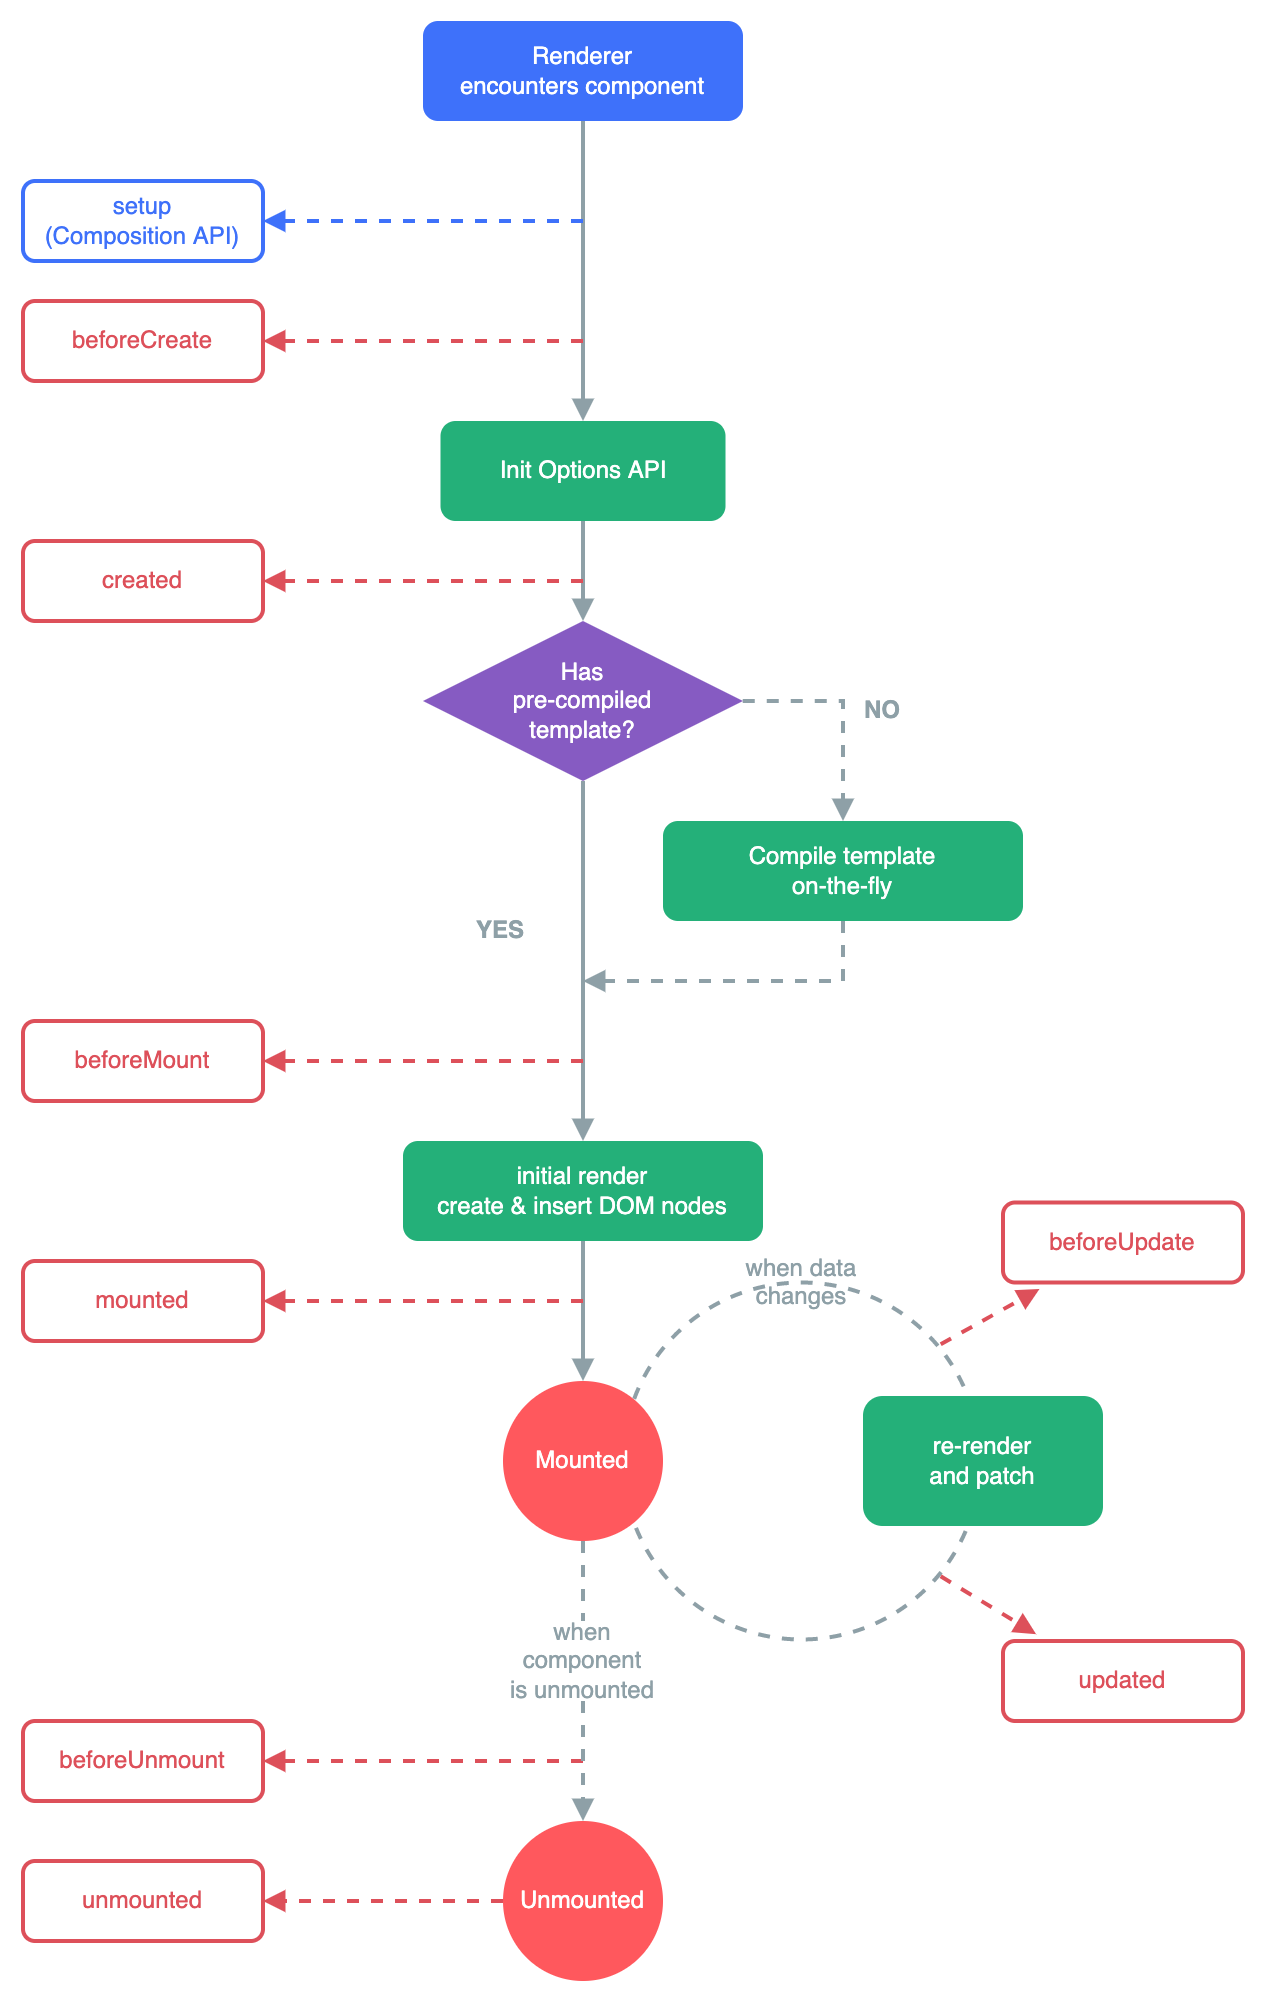
\includegraphics[scale=0.3]{./img/lifecycle.16e4c08e.png} 
\end{center}

\columnratio{0.55}
\begin{paracol}{2}
\switchcolumn[0]*%%%%%%%
Consult the
\href{https://vuejs.org/api/composition-api-lifecycle.html}{Lifecycle
Hooks API reference} for details on all lifecycle hooks and their
respective use cases.
\switchcolumn
有关所有生命周期钩子及其各自用例的详细信息,请参考\href{https://cn.vuejs.org/api/composition-api-lifecycle.html}{生命周期钩子
API 索引}。
\end{paracol}



\columnratio{0.55}
\begin{paracol}{2}
\switchcolumn[0]*%%%%%%%
\section{Watchers}
\switchcolumn
\section{侦听器}
\switchcolumn[0]*%%%%%%%
\subsection{Basic Example}
\switchcolumn
\subsection{基本示例}
\switchcolumn[0]*%%%%%%%
Computed properties allow us to declaratively compute derived values.
However, there are cases where we need to perform "side effects" in
reaction to state changes - for example, mutating the DOM, or changing
another piece of state based on the result of an async operation.
\switchcolumn
计算属性允许我们声明性地计算衍生值。然而在有些情况下,我们需要在状态变化时执行一些``副作用'':例如更改
DOM,或是根据异步操作的结果去修改另一处的状态。

\switchcolumn[0]*%%%%%%%
With Composition API, we can use the
\href{https://vuejs.org/api/reactivity-core.html\#watch}{\texttt{watch}
function} to trigger a callback whenever a piece of reactive state
changes:
\switchcolumn
在组合式 API 中,我们可以使用
\href{https://cn.vuejs.org/api/reactivity-core.html\#watch}{\texttt{watch}
函数}在每次响应式状态发生变化时触发回调函数:
\switchcolumn[0]*%%%%%%%
\begin{codeHtml}
<script setup>
import { ref, watch } from 'vue'
//
const question = ref('')
const answer = ref('Questions usually contain a question mark. ;-)')
//
// 可以直接侦听一个 ref
watch(question, async (newQuestion, oldQuestion) => {
  if (newQuestion.indexOf('?') > -1) {
    answer.value = 'Thinking...'
    try {
      const res = await fetch('https://yesno.wtf/api')
      answer.value = (await res.json()).answer
    } catch (error) {
      answer.value = 'Error! Could not reach the API. ' + error
    }
  }
})
</script>
//
<template>
  <p>
    Ask a yes/no question:
    <input v-model="question" />
  </p>
  <p>{{ answer }}</p>
</template>
\end{codeHtml}
\switchcolumn
\begin{codeHtml}
<script setup>
import { ref, watch } from 'vue'
//
const question = ref('')
const answer = ref('Questions usually contain a question mark. ;-)')
//
// 可以直接侦听一个 ref
watch(question, async (newQuestion, oldQuestion) => {
  if (newQuestion.indexOf('?') > -1) {
    answer.value = 'Thinking...'
    try {
      const res = await fetch('https://yesno.wtf/api')
      answer.value = (await res.json()).answer
    } catch (error) {
      answer.value = 'Error! Could not reach the API. ' + error
    }
  }
})
</script>
//
<template>
  <p>
    Ask a yes/no question:
    <input v-model="question" />
  </p>
  <p>{{ answer }}</p>
</template>
\end{codeHtml}
\switchcolumn[0]*%%%%%%%
\href{https://play.vuejs.org/\#eNp9U8Fy0zAQ/ZVFF9tDah96C2mZ0umhHKBAj7oIe52oUSQjyXEyGf87KytyoDC9JPa+p+e3b1cndtd15b5HtmQrV1vZeXDo++6Wa7nrjPVwAovtAgbh6w2M0Fqzg4xOZFxzXRvtPPzq0XlpNNwEbp5lRUKEdgPaVP925jnoXS+UOgKxvJAaxEVjJ+y2hA9XxUVFGdFIvT7LtEI5JIzrqjrbGozdOmikxdqTKqmIQOV6gvOkvQDhjrqGXOOQvCzAqCa9FHBzCyeuAWT7F6uUulZ9gy7PPmZFETmQjJV7oXoke972GJHY+Axkzxupt4FalhRcYHh7TDIQcqA+LTriikFIDy0G59nG+84tq+qITpty8G0lOhmSiedefSaPZ0mnfHFG50VRRkbkj1BPceVorbFzF/+6fQj4O7g3vWpAm6Ao6JzfINw9PZaQwXuYNJJuK/U0z1nxdTLT0M7s8Ec/I3WxquLS0brRi8ddp4RHegNYhR0M/Du3pXFSAJU285osI7aSuus97K92pkF1w1nCOYNlI534qbCh8tkOVasoXkV1+sjplLZ0HGN5Vc1G2IJ5R8Np5XpKlK7J1CJntdl1UqH92k0bzdkyNc8ZRWGGz1MtbMQi1esN1tv/1F/cIdQ4e6LJod0jZzPmhV2jj/DDjy94oOcZpK57Rew3wO/ojOpjJIH2qdcN2f6DN7l9nC47RfTsHg4etUtNpZUeJz5ndPPv32j9Yve6vE6DZuNvu1R2Tg==}{Try
it in the Playground}
\switchcolumn
\href{https://play.vuejs.org/\#eNplkkGPmzAQhf/KKxdA3Rj1mpJUUdVDT22lHrlYxDRuYOzaJjRC/PcdxyGr3b2A7PfmmzcMc3awVlxGlW2z2rdO2wCvwmj3DenBGhcww6nuCZMM7QkLOmcG5FyRN9RQa8gH/BuVD9oQdtFb5Hm5KpL8pNx6/+vu8xj9KPv+CnYFqQnyhTFIdxb4vCkjpaFb32JVnyD9lVoUpKaVVmK3x9wQoLtXgtB0VP9/cOMveYk9Np/K5MM9l7jIflScLv990nTW9EcIwXNFR3DX1YwYk4dxyrNXTlIHdCrGyk8hWL+tqqvyZMQUukpaHYOnujdtilTLHPHXGyrKUiRH8i9obx+5UM4Z98j6Pu23qH/AVzP2R5CJRMl14aRw+PldIMdH3Bh3bnzxY+FcdZW2zPvlQ1CD7WVQfALquPToP/gzL4RHqsg89rJNWq3JjgGXzWCOqt812ao3GaqEqRKHcfO8/gDLkq7r6tEyW54Bf5TTlg==}{在演练场中尝试一下}


\switchcolumn[0]*%%%%%%%
\subsubsection{Watch Source Types}
\switchcolumn
\subsubsection{侦听数据源类型}
\switchcolumn[0]*%%%%%%%
\texttt{watch}'s first argument can be different types of reactive
"sources": it can be a ref (including computed refs), a reactive object,
a getter function, or an array of multiple sources:
\switchcolumn
\texttt{watch} 的第一个参数可以是不同形式的``数据源'':它可以是一个 ref
(包括计算属性)、一个响应式对象、一个 getter
函数、或多个数据源组成的数组:
\switchcolumn[0]*%%%%%%%
\begin{codeJs}
const x = ref(0)
const y = ref(0)
//
// 单个 ref
watch(x, (newX) => {
  console.log(`x is ${newX}`)
})
//
// getter 函数
watch(
  () => x.value + y.value,
  (sum) => {
    console.log(`sum of x + y is: ${sum}`)
  }
)
//
// 多个来源组成的数组
watch([x, () => y.value], ([newX, newY]) => {
  console.log(`x is ${newX} and y is ${newY}`)
})
\end{codeJs}
\switchcolumn
\begin{codeJs}
const x = ref(0)
const y = ref(0)
//
// 单个 ref
watch(x, (newX) => {
  console.log(`x is ${newX}`)
})
//
// getter 函数
watch(
  () => x.value + y.value,
  (sum) => {
    console.log(`sum of x + y is: ${sum}`)
  }
)
//
// 多个来源组成的数组
watch([x, () => y.value], ([newX, newY]) => {
  console.log(`x is ${newX} and y is ${newY}`)
})
\end{codeJs}


\switchcolumn[0]*%%%%%%%
Do note that you can't watch a property of a reactive object like this:
\switchcolumn
注意,你不能直接侦听响应式对象的属性值,例如:
\switchcolumn[0]*%%%%%%%
\begin{codeJs}
const obj = reactive({ count: 0 })
//
// 错误,因为 watch() 得到的参数是一个 number
watch(obj.count, (count) => {
  console.log(`count is: ${count}`)
})
\end{codeJs}
\switchcolumn
\begin{codeJs}
const obj = reactive({ count: 0 })
//
// 错误,因为 watch() 得到的参数是一个 number
watch(obj.count, (count) => {
  console.log(`count is: ${count}`)
})
\end{codeJs}
\switchcolumn[0]*%%%%%%%
Instead, use a getter:
\switchcolumn
这里需要用一个返回该属性的 getter 函数:


\switchcolumn[0]*%%%%%%%
\begin{codeJs}
// 提供一个 getter 函数
watch(
  () => obj.count,
  (count) => {
    console.log(`count is: ${count}`)
  }
)
\end{codeJs}
\switchcolumn
\begin{codeJs}
// 提供一个 getter 函数
watch(
  () => obj.count,
  (count) => {
    console.log(`count is: ${count}`)
  }
)
\end{codeJs}
\end{paracol}

\columnratio{0.55}
\begin{paracol}{2}

\switchcolumn[0]*%%%%%%%
\subsection{Deep Watchers}
\switchcolumn
\subsection{深层侦听器}
\switchcolumn[0]*%%%%%%%
When you call \texttt{watch()} directly on a reactive object, it will
implicitly create a deep watcher - the callback will be triggered on all
nested mutations:
\switchcolumn
直接给 \texttt{watch()}
传入一个响应式对象,会隐式地创建一个深层侦听器------该回调函数在所有嵌套的变更时都会被触发:
\switchcolumn[0]*%%%%%%%
\begin{codeJs}
const obj = reactive({ count: 0 })
//
watch(obj, (newValue, oldValue) => {
    // 在嵌套的属性变更时触发
    // 注意:`newValue` 此处和 `oldValue` 是相等的
    // 因为它们是同一个对象!
})
//
obj.count++
\end{codeJs}
\switchcolumn
\begin{codeJs}
const obj = reactive({ count: 0 })
//
watch(obj, (newValue, oldValue) => {
    // 在嵌套的属性变更时触发
    // 注意:`newValue` 此处和 `oldValue` 是相等的
    // 因为它们是同一个对象!
})
//
obj.count++
\end{codeJs}


\switchcolumn[0]*%%%%%%%
This should be differentiated with a getter that returns a reactive
object - in the latter case, the callback will only fire if the getter
returns a different object:
\switchcolumn
相比之下,一个返回响应式对象的 getter
函数,只有在返回不同的对象时,才会触发回调:
\switchcolumn[0]*%%%%%%%
\begin{codeJs}
watch(
  () => state.someObject,
  () => {
    // 仅当 state.someObject 被替换时触发
  }
)
\end{codeJs}
\switchcolumn
\begin{codeJs}
watch(
  () => state.someObject,
  () => {
    // 仅当 state.someObject 被替换时触发
  }
)
\end{codeJs}
\switchcolumn[0]*%%%%%%%
You can, however, force the second case into a deep watcher by
explicitly using the \texttt{deep} option:
\switchcolumn
你也可以给上面这个例子显式地加上 \texttt{deep}
选项,强制转成深层侦听器:


\switchcolumn[0]*%%%%%%%
\begin{codeJs}
watch(
  () => state.someObject,
  (newValue, oldValue) => {
    // 注意:`newValue` 此处和 `oldValue` 是相等的
    // *除非* state.someObject 被整个替换了
  },
  { deep: true }
)
\end{codeJs}
\switchcolumn
\begin{codeJs}
watch(
  () => state.someObject,
  (newValue, oldValue) => {
    // 注意:`newValue` 此处和 `oldValue` 是相等的
    // *除非* state.someObject 被整个替换了
  },
  { deep: true }
)
\end{codeJs}
\switchcolumn[0]*%%%%%%%
\begin{vueQuoteWarn}{Use with Caution}
Deep watch requires traversing all nested properties in the watched
object, and can be expensive when used on large data structures. Use it
only when necessary and beware of the performance implications.
\end{vueQuoteWarn}
\switchcolumn
\begin{vueQuoteWarn}{谨慎使用}
深度侦听需要遍历被侦听对象中的所有嵌套的属性,当用于大型数据结构时,开销很大。因此请只在必要时才使用它,并且要留意性能。
\end{vueQuoteWarn}
\end{paracol}

\columnratio{0.55}
\begin{paracol}{2}

\switchcolumn[0]*%%%%%%%
\subsection{Eager Watchers}
\switchcolumn
\subsection{即时回调的侦听器}
\switchcolumn[0]*%%%%%%%
\texttt{watch} is lazy by default: the callback won't be called until
the watched source has changed. But in some cases we may want the same
callback logic to be run eagerly - for example, we may want to fetch
some initial data, and then re-fetch the data whenever relevant state
changes.
\switchcolumn
\texttt{watch}
默认是懒执行的:仅当数据源变化时,才会执行回调。但在某些场景中,我们希望在创建侦听器时,立即执行一遍回调。举例来说,我们想请求一些初始数据,然后在相关状态更改时重新请求数据。
\switchcolumn[0]*%%%%%%%
We can force a watcher's callback to be executed immediately by passing
the \texttt{immediate:\ true} option:
\switchcolumn
我们可以通过传入 \texttt{immediate:\ true}
选项来强制侦听器的回调立即执行:
\switchcolumn[0]*%%%%%%%
\begin{codeJs}
watch(source, (newValue, oldValue) => {
    // 立即执行,且当 `source` 改变时再次执行
}, { immediate: true })
\end{codeJs}
\switchcolumn
\begin{codeJs}
watch(source, (newValue, oldValue) => {
    // 立即执行,且当 `source` 改变时再次执行
}, { immediate: true })
\end{codeJs}
\switchcolumn[0]*%%%%%%%
\subsection{watchEffect()}
\switchcolumn
\subsection{watchEffect()}



\switchcolumn[0]*%%%%%%%
It is common for the watcher callback to use exactly the same reactive
state as the source. For example, consider the following code, which
uses a watcher to load a remote resource whenever the \texttt{todoId}
ref changes:
\switchcolumn
侦听器的回调使用与源完全相同的响应式状态是很常见的。例如下面的代码,在每当
\texttt{todoId} 的引用发生变化时使用侦听器来加载一个远程资源:
\switchcolumn[0]*%%%%%%%
\begin{codeJs}
const todoId = ref(1)
const data = ref(null)
//
watch(todoId, async () => {
  const response = await fetch(
    `https://jsonplaceholder.typicode.com/todos/${todoId.value}`
  )
  data.value = await response.json()
}, { immediate: true })
\end{codeJs}
\switchcolumn
\begin{codeJs}
const todoId = ref(1)
const data = ref(null)
//
watch(todoId, async () => {
  const response = await fetch(
    `https://jsonplaceholder.typicode.com/todos/${todoId.value}`
  )
  data.value = await response.json()
}, { immediate: true })
\end{codeJs}
\switchcolumn[0]*%%%%%%%
In particular, notice how the watcher uses \texttt{todoId} twice, once
as the source and then again inside the callback.
\switchcolumn
特别是注意侦听器是如何两次使用 \texttt{todoId}
的,一次是作为源,另一次是在回调中。
\switchcolumn[0]*%%%%%%%
This can be simplified with
\href{https://vuejs.org/api/reactivity-core.html\#watcheffect}{\texttt{watchEffect()}}.
\texttt{watchEffect()} allows us to track the callback's reactive
dependencies automatically. The watcher above can be rewritten as:
\switchcolumn
我们可以用
\href{https://cn.vuejs.org/api/reactivity-core.html\#watcheffect}{\texttt{watchEffect}
函数} 来简化上面的代码。\texttt{watchEffect()}
允许我们自动跟踪回调的响应式依赖。上面的侦听器可以重写为:
\switchcolumn[0]*%%%%%%%
\begin{codeJs}
watchEffect(async () => {
  const response = await fetch(
    `https://jsonplaceholder.typicode.com/todos/${todoId.value}`
  )
  data.value = await response.json()
})
\end{codeJs}
\switchcolumn
\begin{codeJs}
watchEffect(async () => {
  const response = await fetch(
    `https://jsonplaceholder.typicode.com/todos/${todoId.value}`
  )
  data.value = await response.json()
})
\end{codeJs}


\switchcolumn[0]*%%%%%%%
Here, the callback will run immediately, there's no need to specify
\texttt{immediate:\ true}. During its execution, it will automatically
track \texttt{todoId.value} as a dependency (similar to computed
properties). Whenever \texttt{todoId.value} changes, the callback will
be run again. With \texttt{watchEffect()}, we no longer need to pass
\texttt{todoId} explicitly as the source value.
\switchcolumn
这个例子中,回调会立即执行,不需要指定
\texttt{immediate:\ true}。在执行期间,它会自动追踪
\texttt{todoId.value} 作为依赖(和计算属性类似)。每当
\texttt{todoId.value} 变化时,回调会再次执行。有了
\texttt{watchEffect()},我们不再需要明确传递 \texttt{todoId} 作为源值。
\switchcolumn[0]*%%%%%%%
You can check out \href{https://vuejs.org/examples/\#fetching-data}{this
example} of \texttt{watchEffect()} and reactive data-fetching in action.
\switchcolumn
你可以参考一下\href{https://cn.vuejs.org/examples/\#fetching-data}{这个例子}的
\texttt{watchEffect} 和响应式的数据请求的操作。
\switchcolumn[0]*%%%%%%%
For examples like these, with only one dependency, the benefit of
\texttt{watchEffect()} is relatively small. But for watchers that have
multiple dependencies, using \texttt{watchEffect()} removes the burden
of having to maintain the list of dependencies manually. In addition, if
you need to watch several properties in a nested data structure,
\texttt{watchEffect()} may prove more efficient than a deep watcher, as
it will only track the properties that are used in the callback, rather
than recursively tracking all of them.
\switchcolumn
对于这种只有一个依赖项的例子来说,\texttt{watchEffect()}
的好处相对较小。但是对于有多个依赖项的侦听器来说,使用
\texttt{watchEffect()}
可以消除手动维护依赖列表的负担。此外,如果你需要侦听一个嵌套数据结构中的几个属性,\texttt{watchEffect()}
可能会比深度侦听器更有效,因为它将只跟踪回调中被使用到的属性,而不是递归地跟踪所有的属性。
\switchcolumn[0]*%%%%%%%
\begin{vueQuote}{TIP}
\texttt{watchEffect} only tracks dependencies during its
\textbf{synchronous} execution. When using it with an async callback,
only properties accessed before the first \texttt{await} tick will be
tracked.
\end{vueQuote}
\switchcolumn
\begin{vueQuote}{TIP}
\texttt{watchEffect}
仅会在其\textbf{同步}执行期间,才追踪依赖。在使用异步回调时,只有在第一个
\texttt{await} 正常工作前访问到的属性才会被追踪。
\end{vueQuote}
\end{paracol}

\columnratio{0.55}
\begin{paracol}{2}

\switchcolumn[0]*%%%%%%%
\subsubsection{watch vs. watchEffect}
\switchcolumn
\subsubsection{watch vs. watchEffect}
\switchcolumn[0]*%%%%%%%
\texttt{watch} and \texttt{watchEffect} both allow us to reactively
perform side effects. Their main difference is the way they track their
reactive dependencies:
\switchcolumn
\texttt{watch} 和 \texttt{watchEffect}
都能响应式地执行有副作用的回调。它们之间的主要区别是追踪响应式依赖的方式:
\switchcolumn[0]*%%%%%%%
\begin{itemize}
\item
    \texttt{watch} only tracks the explicitly watched source. It won't
    track anything accessed inside the callback. In addition, the callback
    only triggers when the source has actually changed. \texttt{watch}
    separates dependency tracking from the side effect, giving us more
    precise control over when the callback should fire.
\item
    \texttt{watchEffect}, on the other hand, combines dependency tracking
    and side effect into one phase. It automatically tracks every reactive
    property accessed during its synchronous execution. This is more
    convenient and typically results in terser code, but makes its
    reactive dependencies less explicit.
\end{itemize}
\switchcolumn
\begin{itemize}
\item
    \texttt{watch}
    只追踪明确侦听的数据源。它不会追踪任何在回调中访问到的东西。另外,仅在数据源确实改变时才会触发回调。\texttt{watch}
    会避免在发生副作用时追踪依赖,因此,我们能更加精确地控制回调函数的触发时机。
\item
    \texttt{watchEffect},则会在副作用发生期间追踪依赖。它会在同步执行过程中,自动追踪所有能访问到的响应式属性。这更方便,而且代码往往更简洁,但有时其响应性依赖关系会不那么明确。
\end{itemize}
\switchcolumn[0]*%%%%%%%
\subsection{Callback Flush Timing}
\switchcolumn
\subsection{回调的触发时机}


\switchcolumn[0]*%%%%%%%
When you mutate reactive state, it may trigger both Vue component
updates and watcher callbacks created by you.
\switchcolumn
当你更改了响应式状态,它可能会同时触发 Vue 组件更新和侦听器回调。
\switchcolumn[0]*%%%%%%%
By default, user-created watcher callbacks are called \textbf{before}
Vue component updates. This means if you attempt to access the DOM
inside a watcher callback, the DOM will be in the state before Vue has
applied any updates.
\switchcolumn
默认情况下,用户创建的侦听器回调,都会在 Vue
组件更新\textbf{之前}被调用。这意味着你在侦听器回调中访问的 DOM 将是被
Vue 更新之前的状态。
\switchcolumn[0]*%%%%%%%
If you want to access the DOM in a watcher callback \textbf{after} Vue
has updated it, you need to specify the
\texttt{flush:\ \textquotesingle{}post\textquotesingle{}} option:
\switchcolumn
如果想在侦听器回调中能访问被 Vue 更新\textbf{之后}的 DOM,你需要指明
\texttt{flush:\ \textquotesingle{}post\textquotesingle{}} 选项:
\switchcolumn[0]*%%%%%%%
\begin{codeJs}
watch(source, callback, {
  flush: 'post'
})
//
watchEffect(callback, {
  flush: 'post'
})
\end{codeJs}
\switchcolumn
\begin{codeJs}
watch(source, callback, {
  flush: 'post'
})
//
watchEffect(callback, {
  flush: 'post'
})
\end{codeJs}


\switchcolumn[0]*%%%%%%%
Post-flush \texttt{watchEffect()} also has a convenience alias,
\texttt{watchPostEffect()}:
\switchcolumn
后置刷新的 \texttt{watchEffect()} 有个更方便的别名
\texttt{watchPostEffect()}:
\switchcolumn[0]*%%%%%%%
\begin{codeJs}
import { watchPostEffect } from 'vue'
//
watchPostEffect(() => {
  /* 在 Vue 更新后执行 */
})
\end{codeJs}
\switchcolumn
\begin{codeJs}
import { watchPostEffect } from 'vue'
//
watchPostEffect(() => {
  /* 在 Vue 更新后执行 */
})
\end{codeJs}
\end{paracol}

\columnratio{0.55}
\begin{paracol}{2}

\switchcolumn[0]*%%%%%%%
\subsection{Stopping a Watcher}
\switchcolumn
\subsection{停止侦听器}
\switchcolumn[0]*%%%%%%%
Watchers declared synchronously inside \texttt{setup()} or
\texttt{\textless{}script\ setup\textgreater{}} are bound to the owner
component instance, and will be automatically stopped when the owner
component is unmounted. In most cases, you don't need to worry about
stopping the watcher yourself.
\switchcolumn
在 \texttt{setup()} 或 \texttt{\textless{}script\ setup\textgreater{}}
中用同步语句创建的侦听器,会自动绑定到宿主组件实例上,并且会在宿主组件卸载时自动停止。因此,在大多数情况下,你无需关心怎么停止一个侦听器。
\switchcolumn[0]*%%%%%%%
The key here is that the watcher must be created \textbf{synchronously}:
if the watcher is created in an async callback, it won't be bound to the
owner component and must be stopped manually to avoid memory leaks.
Here's an example:
\switchcolumn
一个关键点是,侦听器必须用\textbf{同步}语句创建:如果用异步回调创建一个侦听器,那么它不会绑定到当前组件上,你必须手动停止它,以防内存泄漏。如下方这个例子:
\switchcolumn[0]*%%%%%%%
\begin{codeHtml}
<script setup>
import { watchEffect } from 'vue'
//
// 它会自动停止
watchEffect(() => {})
//
// ...这个则不会!
setTimeout(() => {
    watchEffect(() => {})
}, 100)
</script>
\end{codeHtml}
\switchcolumn
\begin{codeHtml}
<script setup>
import { watchEffect } from 'vue'
//
// 它会自动停止
watchEffect(() => {})
//
// ...这个则不会!
setTimeout(() => {
    watchEffect(() => {})
}, 100)
</script>
\end{codeHtml}
\switchcolumn[0]*%%%%%%%
To manually stop a watcher, use the returned handle function. This works
for both \texttt{watch} and \texttt{watchEffect}:
\switchcolumn
要手动停止一个侦听器,请调用 \texttt{watch} 或 \texttt{watchEffect}
返回的函数:


\switchcolumn[0]*%%%%%%%
\begin{codeJs}
const unwatch = watchEffect(() => {})
//
// ...当该侦听器不再需要时
unwatch()
\end{codeJs}
\switchcolumn
\begin{codeJs}
const unwatch = watchEffect(() => {})
//
// ...当该侦听器不再需要时
unwatch()
\end{codeJs}
\switchcolumn[0]*%%%%%%%
Note that there should be very few cases where you need to create
watchers asynchronously, and synchronous creation should be preferred
whenever possible. If you need to wait for some async data, you can make
your watch logic conditional instead:
\switchcolumn
注意,需要异步创建侦听器的情况很少,请尽可能选择同步创建。如果需要等待一些异步数据,你可以使用条件式的侦听逻辑:
\switchcolumn[0]*%%%%%%%
\begin{codeJs}
// 需要异步请求得到的数据
const data = ref(null)
//
watchEffect(() => {
  if (data.value) {
    // 数据加载后执行某些操作...
  }
})
\end{codeJs}
\switchcolumn
\begin{codeJs}
// 需要异步请求得到的数据
const data = ref(null)
//
watchEffect(() => {
  if (data.value) {
    // 数据加载后执行某些操作...
  }
})
\end{codeJs}
\end{paracol}


\columnratio{0.55}
\begin{paracol}{2}

\switchcolumn[0]*%%%%%%%
\section{Template Refs}
\switchcolumn
\section{模板引用}
\switchcolumn[0]*%%%%%%%
While Vue's declarative rendering model abstracts away most of the
direct DOM operations for you, there may still be cases where we need
direct access to the underlying DOM elements. To achieve this, we can
use the special \texttt{ref} attribute:
\switchcolumn
虽然 Vue 的声明性渲染模型为你抽象了大部分对 DOM
的直接操作,但在某些情况下,我们仍然需要直接访问底层 DOM
元素。要实现这一点,我们可以使用特殊的 \texttt{ref} attribute:
\switchcolumn[0]*%%%%%%%
\begin{codeHtml}
<input ref="input">
\end{codeHtml}
\switchcolumn
\begin{codeHtml}
<input ref="input">
\end{codeHtml}

\switchcolumn[0]*%%%%%%%
\texttt{ref} is a special attribute, similar to the \texttt{key}
attribute discussed in the \texttt{v-for} chapter. It allows us to
obtain a direct reference to a specific DOM element or child component
instance after it's mounted. This may be useful when you want to, for
example, programmatically focus an input on component mount, or
initialize a 3rd party library on an element.
\switchcolumn
\texttt{ref} 是一个特殊的 attribute,和 \texttt{v-for} 章节中提到的
\texttt{key} 类似。它允许我们在一个特定的 DOM
元素或子组件实例被挂载后,获得对它的直接引用。这可能很有用,比如说在组件挂载时将焦点设置到一个
input 元素上,或在一个元素上初始化一个第三方库。


\switchcolumn[0]*%%%%%%%
\subsection{Accessing the Refs}
\switchcolumn
\subsection{访问模板引用}
\switchcolumn[0]*%%%%%%%
To obtain the reference with Composition API, we need to declare a ref
with the same name:
\switchcolumn
为了通过组合式 API 获得该模板引用,我们需要声明一个同名的 ref:
\switchcolumn[0]*%%%%%%%
\begin{codeHtml}
<script setup>
import { ref, onMounted } from 'vue'
//
// 声明一个 ref 来存放该元素的引用
// 必须和模板里的 ref 同名
const input = ref(null)
//
onMounted(() => {
  input.value.focus()
})
</script>
//
<template>
  <input ref="input" />
</template>
\end{codeHtml}
\switchcolumn
\begin{codeHtml}
<script setup>
import { ref, onMounted } from 'vue'
//
// 声明一个 ref 来存放该元素的引用
// 必须和模板里的 ref 同名
const input = ref(null)
//
onMounted(() => {
  input.value.focus()
})
</script>
//
<template>
  <input ref="input" />
</template>
\end{codeHtml}


\switchcolumn[0]*%%%%%%%
If not using \texttt{\textless{}script\ setup\textgreater{}}, make sure
to also return the ref from \texttt{setup()}:
\switchcolumn
如果不使用 \texttt{\textless{}script\ setup\textgreater{}},需确保从
\texttt{setup()} 返回 ref:
\switchcolumn[0]*%%%%%%%
\begin{codeJs}
export default {
  setup() {
    const input = ref(null)
    // ...
    return {
      input
    }
  }
}
\end{codeJs}
\switchcolumn
\begin{codeJs}
export default {
  setup() {
    const input = ref(null)
    // ...
    return {
      input
    }
  }
}
\end{codeJs}
\switchcolumn[0]*%%%%%%%
Note that you can only access the ref \textbf{after the component is
mounted.} If you try to access \texttt{input} in a template expression,
it will be \texttt{null} on the first render. This is because the
element doesn't exist until after the first render!
\switchcolumn
注意,你只可以\textbf{在组件挂载后}才能访问模板引用。如果你想在模板中的表达式上访问
\texttt{input},在初次渲染时会是
\texttt{null}。这是因为在初次渲染前这个元素还不存在呢!


\switchcolumn[0]*%%%%%%%
If you are trying to watch the changes of a template ref, make sure to
account for the case where the ref has \texttt{null} value:
\switchcolumn
如果你需要侦听一个模板引用 ref 的变化,确保考虑到其值为 \texttt{null}
的情况:
\switchcolumn[0]*%%%%%%%
\begin{codeJs}
watchEffect(() => {
  if (input.value) {
    input.value.focus()
  } else {
    // 此时还未挂载,或此元素已经被卸载(例如通过 v-if 控制)
  }
})
\end{codeJs}
\switchcolumn
\begin{codeJs}
watchEffect(() => {
  if (input.value) {
    input.value.focus()
  } else {
    // 此时还未挂载,或此元素已经被卸载(例如通过 v-if 控制)
  }
})
\end{codeJs}
\switchcolumn[0]*%%%%%%%
See also:
\href{https://vuejs.org/guide/typescript/composition-api.html\#typing-template-refs}{Typing
Template Refs}
\switchcolumn
也可参考:\href{https://cn.vuejs.org/guide/typescript/composition-api.html\#typing-template-refs}{为模板引用标注类型}


\switchcolumn[0]*%%%%%%%
\subsection{Refs inside v-for}
\switchcolumn
\subsection{v-for 中的模板引用}
\switchcolumn[0]*%%%%%%%
\begin{quote}
Requires v3.2.25 or above
\end{quote}
\switchcolumn
\begin{quote}
需要 v3.2.25 及以上版本
\end{quote}
\switchcolumn[0]*%%%%%%%
When \texttt{ref} is used inside \texttt{v-for}, the corresponding ref
should contain an Array value, which will be populated with the elements
after mount:
\switchcolumn
当在 \texttt{v-for} 中使用模板引用时,对应的 ref
中包含的值是一个数组,它将在元素被挂载后包含对应整个列表的所有元素:


\switchcolumn[0]*%%%%%%%
\begin{codeHtml}
<script setup>
import { ref, onMounted } from 'vue'
//
const list = ref([
  /* ... */
])
//
const itemRefs = ref([])
//
onMounted(() => console.log(itemRefs.value))
</script>
<!-- -->
<template>
  <ul>
    <li v-for="item in list" ref="itemRefs">
      {{ item }}
    </li>
  </ul>
</template>
\end{codeHtml}
\switchcolumn
\begin{codeHtml}
<script setup>
import { ref, onMounted } from 'vue'
//
const list = ref([
  /* ... */
])
//
const itemRefs = ref([])
//
onMounted(() => console.log(itemRefs.value))
</script>
<!-- -->
<template>
  <ul>
    <li v-for="item in list" ref="itemRefs">
      {{ item }}
    </li>
  </ul>
</template>
\end{codeHtml}
\switchcolumn[0]*%%%%%%%
\href{https://play.vuejs.org/\#eNpFjs1qwzAQhF9l0CU2uDZtb8UOlJ576bXqwaQyCGRJyCsTEHr3rGwnOehnd2e+nSQ+vW/XqMSH6JdL0J6wKIr+LK2evQuEhKCmBs5+u2hJ/SNjCm7GiV0naaW9OLsQjOZrKNrq97XBW4P3v/o51qTmHzUtd8k+e0CrqsZwRpIWGI0KVN0N7TqaqNp59JUuEt2SutKXY5elmimZT9/t2Tk1F+z0ZiTFFdBHs738Mxrry+TCIEWhQ9sttRQl0tEsK6U4HEBKW3LkfDA6o3dst3H77rFM5BtTfm/P}{Try
it in the Playground}
\switchcolumn
\href{https://play.vuejs.org/\#eNpFjs1qwzAQhF9l0CU2uDZtb8UOlJ576bXqwaQyCGRJyCsTEHr3rGwnOehnd2e+nSQ+vW/XqMSH6JdL0J6wKIr+LK2evQuEhKCmBs5+u2hJ/SNjCm7GiV0naaW9OLsQjOZrKNrq97XBW4P3v/o51qTmHzUtd8k+e0CrqsZwRpIWGI0KVN0N7TqaqNp59JUuEt2SutKXY5elmimZT9/t2Tk1F+z0ZiTFFdBHs738Mxrry+TCIEWhQ9sttRQl0tEsK6U4HEBKW3LkfDA6o3dst3H77rFM5BtTfm/P}{在演练场中尝试一下}
\switchcolumn[0]*%%%%%%%
It should be noted that the ref array does \textbf{not} guarantee the
same order as the source array.
\switchcolumn
应该注意的是,ref 数组\textbf{并不}保证与源数组相同的顺序。


\switchcolumn[0]*%%%%%%% 
\subsection{Function Refs}
\switchcolumn
\subsection{函数模板引用}
\switchcolumn[0]*%%%%%%%
Instead of a string key, the \texttt{ref} attribute can also be bound to
a function, which will be called on each component update and gives you
full flexibility on where to store the element reference. The function
receives the element reference as the first argument:
\switchcolumn
除了使用字符串值作名字,\texttt{ref} attribute
还可以绑定为一个函数,会在每次组件更新时都被调用。该函数会收到元素引用作为其第一个参数:
\switchcolumn[0]*%%%%%%%
\begin{codeHtml}
<input :ref="(el) => { /* 将 el 赋值给一个数据属性或 ref 变量 */ }">
\end{codeHtml}
\switchcolumn
\begin{codeHtml}
<input :ref="(el) => { /* 将 el 赋值给一个数据属性或 ref 变量 */ }">
\end{codeHtml}


\switchcolumn[0]*%%%%%%%
Note we are using a dynamic \texttt{:ref} binding so we can pass it a
function instead of a ref name string. When the element is unmounted,
the argument will be \texttt{null}. You can, of course, use a method
instead of an inline function.
\switchcolumn
注意我们这里需要使用动态的 \texttt{:ref}
绑定才能够传入一个函数。当绑定的元素被卸载时,函数也会被调用一次,此时的
\texttt{el} 参数会是
\texttt{null}。你当然也可以绑定一个组件方法而不是内联函数。
\switchcolumn[0]*%%%%%%%
\subsection{Ref on Component}
\switchcolumn
\subsection{组件上的 ref}
\switchcolumn[0]*%%%%%%%
\begin{quote}
This section assumes knowledge of
\href{https://vuejs.org/guide/essentials/component-basics.html}{Components}.
Feel free to skip it and come back later.
\end{quote}
\switchcolumn
\begin{quote}
这一小节假设你已了解\href{https://cn.vuejs.org/guide/essentials/component-basics.html}{组件}的相关知识,或者你也可以先跳过这里,之后再回来看。
\end{quote}


\switchcolumn[0]*%%%%%%%
\texttt{ref} can also be used on a child component. In this case the
reference will be that of a component instance:
\switchcolumn
模板引用也可以被用在一个子组件上。这种情况下引用中获得的值是组件实例:
\switchcolumn[0]*%%%%%%%
\begin{codeHtml}
<script setup>
import { ref, onMounted } from 'vue'
import Child from './Child.vue'
<!-- -->
const child = ref(null)
<!-- -->
onMounted(() => {
  // child.value 是 <Child /> 组件的实例
})
</script>
<!-- -->
<template>
  <Child ref="child" />
</template>
\end{codeHtml}
\switchcolumn
\begin{codeHtml}
<script setup>
import { ref, onMounted } from 'vue'
import Child from './Child.vue'
<!-- -->
const child = ref(null)
<!-- -->
onMounted(() => {
  // child.value 是 <Child /> 组件的实例
})
</script>
<!-- -->
<template>
  <Child ref="child" />
</template>
\end{codeHtml}
\switchcolumn[0]*%%%%%%%
If the child component is using Options API or not using
\texttt{\textless{}script\ setup\textgreater{}}, the referenced instance
will be identical to the child component's \texttt{this}, which means
the parent component will have full access to every property and method
of the child component. This makes it easy to create tightly coupled
implementation details between the parent and the child, so component
refs should be only used when absolutely needed - in most cases, you
should try to implement parent / child interactions using the standard
props and emit interfaces first.
\switchcolumn
如果一个子组件使用的是选项式 API 或没有使用
\texttt{\textless{}script\ setup\textgreater{}},被引用的组件实例和该子组件的
\texttt{this}
完全一致,这意味着父组件对子组件的每一个属性和方法都有完全的访问权。这使得在父组件和子组件之间创建紧密耦合的实现细节变得很容易,当然也因此,应该只在绝对需要时才使用组件引用。大多数情况下,你应该首先使用标准的
props 和 emit 接口来实现父子组件交互。


\switchcolumn[0]*%%%%%%%
An exception here is that components using
\texttt{\textless{}script\ setup\textgreater{}} are \textbf{private by
default}: a parent component referencing a child component using
\texttt{\textless{}script\ setup\textgreater{}} won't be able to access
anything unless the child component chooses to expose a public interface
using the \texttt{defineExpose} macro:
\switchcolumn
有一个例外的情况,使用了 \texttt{\textless{}script\ setup\textgreater{}}
的组件是\textbf{默认私有}的:一个父组件无法访问到一个使用了
\texttt{\textless{}script\ setup\textgreater{}}
的子组件中的任何东西,除非子组件在其中通过 \texttt{defineExpose}
宏显式暴露:
\switchcolumn[0]*%%%%%%%
\begin{codeHtml}
<script setup>
import { ref } from 'vue'
<!-- -->
const a = 1
const b = ref(2)
<!-- -->
// 像 defineExpose 这样的编译器宏不需要导入
defineExpose({
  a,
  b
})
</script>
\end{codeHtml}
\switchcolumn
\begin{codeHtml}
<script setup>
import { ref } from 'vue'
<!-- -->
const a = 1
const b = ref(2)
<!-- -->
// 像 defineExpose 这样的编译器宏不需要导入
defineExpose({
  a,
  b
})
</script>
\end{codeHtml}
\switchcolumn[0]*%%%%%%%
When a parent gets an instance of this component via template refs, the
retrieved instance will be of the shape
\texttt{\{\ a:\ number,\ b:\ number\ \}} (refs are automatically
unwrapped just like on normal instances).
\switchcolumn
当父组件通过模板引用获取到了该组件的实例时,得到的实例类型为
\texttt{\{\ a:\ number,\ b:\ number\ \}} (ref
都会自动解包,和一般的实例一样)。


\switchcolumn[0]*%%%%%%%
See also:
\href{https://vuejs.org/guide/typescript/composition-api.html\#typing-component-template-refs}{Typing
Component Template Refs}
\switchcolumn
TypeScript
用户请参考:\href{https://cn.vuejs.org/guide/typescript/composition-api.html\#typing-component-template-refs}{为组件的模板引用标注类型}
\end{paracol}
 
\columnratio{0.55}
\begin{paracol}{2}
\switchcolumn[0]*%%%%%%%
\section{Components Basics}
\switchcolumn
\section{组件基础}
\switchcolumn[0]*%%%%%%%
Components allow us to split the UI into independent and reusable
pieces, and think about each piece in isolation. It's common for an app
to be organized into a tree of nested components:
\switchcolumn
组件允许我们将 UI
划分为独立的、可重用的部分,并且可以对每个部分进行单独的思考。在实际应用中,组件常常被组织成层层嵌套的树状结构:
\end{paracol}


\begin{center} 
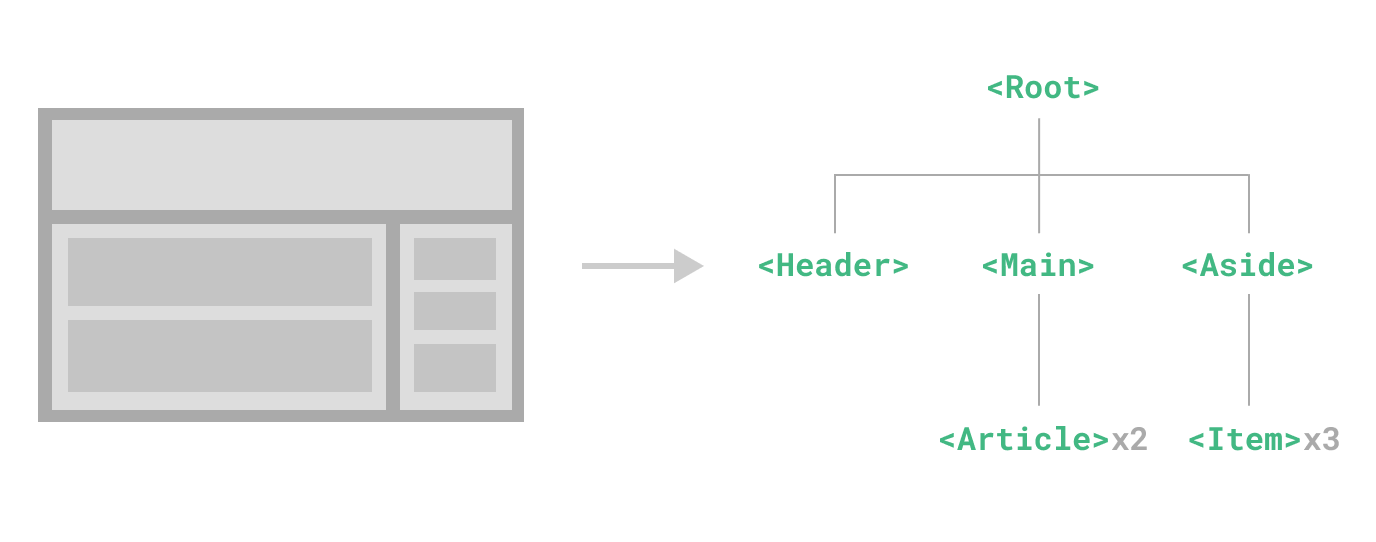
\includegraphics{./img/components.7fbb3771.png} 
\end{center}

\columnratio{0.55}
\begin{paracol}{2}

\switchcolumn[0]*%%%%%%%
This is very similar to how we nest native HTML elements, but Vue
implements its own component model that allow us to encapsulate custom
content and logic in each component. Vue also plays nicely with native
Web Components. If you are curious about the relationship between Vue
Components and native Web Components,
\href{https://vuejs.org/guide/extras/web-components.html}{read more
here}.
\switchcolumn
这和我们嵌套 HTML 元素的方式类似,Vue
实现了自己的组件模型,使我们可以在每个组件内封装自定义内容与逻辑。Vue
同样也能很好地配合原生 Web Component。如果你想知道 Vue 组件与原生 Web
Components
之间的关系,可以\href{https://cn.vuejs.org/guide/extras/web-components.html}{阅读此章节}。
\switchcolumn[0]*%%%%%%%
\subsection{Defining a Component}
\switchcolumn
\subsection{定义一个组件}
\switchcolumn[0]*%%%%%%%
When using a build step, we typically define each Vue component in a
dedicated file using the \texttt{.vue} extension - known as a
\href{https://vuejs.org/guide/scaling-up/sfc.html}{Single-File
Component} (SFC for short):
\switchcolumn
当使用构建步骤时,我们一般会将 Vue 组件定义在一个单独的 \texttt{.vue}
文件中,这被叫做\href{https://cn.vuejs.org/guide/scaling-up/sfc.html}{单文件组件}
(简称 SFC):
\switchcolumn[0]*%%%%%%%
\begin{codeHtml}
<script setup>
import { ref } from 'vue'
//
const count = ref(0)
</script>
//
<template>
    <button @click="count++">You clicked me {{ count }} times.</button>
</template>
\end{codeHtml}
\switchcolumn
\begin{codeHtml}
<script setup>
import { ref } from 'vue'
//
const count = ref(0)
</script>
//
<template>
    <button @click="count++">You clicked me {{ count }} times.</button>
</template>
\end{codeHtml}
\switchcolumn[0]*%%%%%%%
When not using a build step, a Vue component can be defined as a plain
JavaScript object containing Vue-specific options:
\switchcolumn
当不使用构建步骤时,一个 Vue 组件以一个包含 Vue 特定选项的 JavaScript
对象来定义:


\switchcolumn[0]*%%%%%%%
\begin{codeJs}
import { ref } from 'vue'
//
export default {
  setup() {
    const count = ref(0)
    return { count }
  },
  template: `
    <button @click="count++">
      You clicked me {{ count }} times.
    </button>`
  // 也可以针对一个 DOM 内联模板:
  // template: '#my-template-element'
}
\end{codeJs}
\switchcolumn
\begin{codeJs}
import { ref } from 'vue'
//
export default {
  setup() {
    const count = ref(0)
    return { count }
  },
  template: `
    <button @click="count++">
      You clicked me {{ count }} times.
    </button>`
  // 也可以针对一个 DOM 内联模板:
  // template: '#my-template-element'
}
\end{codeJs}
\switchcolumn[0]*%%%%%%%
The template is inlined as a JavaScript string here, which Vue will
compile on the fly. You can also use an ID selector pointing to an
element (usually native \texttt{\textless{}template\textgreater{}}
elements) - Vue will use its content as the template source.
\switchcolumn
这里的模板是一个内联的 JavaScript 字符串,Vue
将会在运行时编译它。你也可以使用 ID 选择器来指向一个元素 (通常是原生的
\texttt{\textless{}template\textgreater{}} 元素),Vue
将会使用其内容作为模板来源。
\switchcolumn[0]*%%%%%%%
The example above defines a single component and exports it as the
default export of a \texttt{.js} file, but you can use named exports to
export multiple components from the same file.
\switchcolumn
上面的例子中定义了一个组件,并在一个 \texttt{.js}
文件里默认导出了它自己,但你也可以通过具名导出在一个文件中导出多个组件。
\switchcolumn[0]*%%%%%%%
\subsection{Using a Component}
\switchcolumn
\subsection{使用组件}
\switchcolumn[0]*%%%%%%%
\begin{vueQuote}{TIP}
We will be using SFC syntax for the rest of this guide - the concepts
around components are the same regardless of whether you are using a
build step or not. The \href{https://vuejs.org/examples/}{Examples}
section shows component usage in both scenarios.
\end{vueQuote}
\switchcolumn
\begin{vueQuote}{TIP}
我们会在接下来的指引中使用 SFC
语法,无论你是否使用构建步骤,组件相关的概念都是相同的。\href{https://cn.vuejs.org/examples/}{示例}一节中展示了两种场景中的组件使用情况。
\end{vueQuote}


\switchcolumn[0]*%%%%%%%
To use a child component, we need to import it in the parent component.
Assuming we placed our counter component inside a file called
\texttt{ButtonCounter.vue}, the component will be exposed as the file's
default export:
\switchcolumn
要使用一个子组件,我们需要在父组件中导入它。假设我们把计数器组件放在了一个叫做
\texttt{ButtonCounter.vue}
的文件中,这个组件将会以默认导出的形式被暴露给外部。
\switchcolumn[0]*%%%%%%%
\begin{codeHtml}
<script setup>
import ButtonCounter from './ButtonCounter.vue'
</script>
<!-- -->
<template>
  <h1>Here is a child component!</h1>
  <ButtonCounter />
</template>
\end{codeHtml}
\switchcolumn
\begin{codeHtml}
<script setup>
import ButtonCounter from './ButtonCounter.vue'
</script>
<!-- -->
<template>
  <h1>Here is a child component!</h1>
  <ButtonCounter />
</template>
\end{codeHtml}
\switchcolumn[0]*%%%%%%%
With \texttt{\textless{}script\ setup\textgreater{}}, imported
components are automatically made available to the template.
\switchcolumn
通过
\texttt{\textless{}script\ setup\textgreater{}},导入的组件都在模板中直接可用。
\switchcolumn[0]*%%%%%%%
It's also possible to globally register a component, making it available
to all components in a given app without having to import it. The pros
and cons of global vs. local registration is discussed in the dedicated
\href{https://vuejs.org/guide/components/registration.html}{Component
Registration} section.
\switchcolumn
当然,你也可以全局地注册一个组件,使得它在当前应用中的任何组件上都可以使用,而不需要额外再导入。关于组件的全局注册和局部注册两种方式的利弊,我们放在了\href{https://cn.vuejs.org/guide/components/registration.html}{组件注册}这一章节中专门讨论。
\switchcolumn[0]*%%%%%%%
Components can be reused as many times as you want:
\switchcolumn
组件可以被重用任意多次:


\switchcolumn[0]*%%%%%%%
\begin{codeHtml}
<h1>Here is a child component!</h1>
<ButtonCounter />
<ButtonCounter />
<ButtonCounter />
\end{codeHtml}
\switchcolumn
\begin{codeHtml}
<h1>Here is a child component!</h1>
<ButtonCounter />
<ButtonCounter />
<ButtonCounter />
\end{codeHtml}
\switchcolumn[0]*%%%%%%%
\href{https://play.vuejs.org/\#eNqVj91KAzEQhV/lmJsqlY3eSlr8ufEVhNys6ZQGNz8kE0GWfXez2SJUsdCLuZiZM9+ZM4qnGLvPQuJBqGySjYxMXOJWe+tiSIznwhz8SyieKWGfgsOqkyfTGbDSXsmFUG9rw+Ti0DPNHavD/faVEqGv5Xr/BXOwww4mVBNPnvOVklXTtKeO8qKhkj++4lb8+fL/mCMS7TEdAy6BtDfBZ65fVgA2s+L67uZMUEC9N0s8msGaj40W7Xa91qKtgbdQ0Ha0gyOM45E+TWDrKHeNIhfMr0DTN4U0me8=}{Try
it in the Playground}
\switchcolumn
\href{https://play.vuejs.org/\#eNqVj91KAzEQhV/lmJsqlY3eSlr8ufEVhNys6ZQGNz8kE0GWfXez2SJUsdCLuZiZM9+ZM4qnGLvPQuJBqGySjYxMXOJWe+tiSIznwhz8SyieKWGfgsOqkyfTGbDSXsmFUG9rw+Ti0DPNHavD/faVEqGv5Xr/BXOwww4mVBNPnvOVklXTtKeO8qKhkj++4lb8+fL/mCMS7TEdAy6BtDfBZ65fVgA2s+L67uZMUEC9N0s8msGaj40W7Xa91qKtgbdQ0Ha0gyOM45E+TWDrKHeNIhfMr0DTN4U0me8=}{在演练场中尝试一下}
\switchcolumn[0]*%%%%%%%
Notice that when clicking on the buttons, each one maintains its own,
separate \texttt{count}. That's because each time you use a component, a
new \textbf{instance} of it is created.
\switchcolumn
你会注意到,每当点击这些按钮时,每一个组件都维护着自己的状态,是不同的
\texttt{count}。这是因为每当你使用一个组件,就创建了一个新的\textbf{实例}。
\switchcolumn[0]*%%%%%%%
In SFCs, it's recommended to use \texttt{PascalCase} tag names for child
components to differentiate from native HTML elements. Although native
HTML tag names are case-insensitive, Vue SFC is a compiled format so we
are able to use case-sensitive tag names in it. We are also able to use
\texttt{/\textgreater{}} to close a tag.
\switchcolumn
在单文件组件中,推荐为子组件使用 \texttt{PascalCase}
的标签名,以此来和原生的 HTML 元素作区分。虽然原生 HTML
标签名是不区分大小写的,但 Vue
单文件组件是可以在编译中区分大小写的。我们也可以使用
\texttt{/\textgreater{}} 来关闭一个标签。
\switchcolumn[0]*%%%%%%%
If you are authoring your templates directly in a DOM (e.g. as the
content of a native \texttt{\textless{}template\textgreater{}} element),
the template will be subject to the browser's native HTML parsing
behavior. In such cases, you will need to use \texttt{kebab-case} and
explicit closing tags for components:
\switchcolumn
如果你是直接在 DOM 中书写模板 (例如原生
\texttt{\textless{}template\textgreater{}}
元素的内容),模板的编译需要遵从浏览器中 HTML
的解析行为。在这种情况下,你应该需要使用 \texttt{kebab-case}
形式并显式地关闭这些组件的标签。


\switchcolumn[0]*%%%%%%%
\begin{codeHtml}
<!-- 如果是在 DOM 中书写该模板 -->
<button-counter></button-counter>
<button-counter></button-counter>
<button-counter></button-counter>
\end{codeHtml}
\switchcolumn
\begin{codeHtml}
<!-- 如果是在 DOM 中书写该模板 -->
<button-counter></button-counter>
<button-counter></button-counter>
<button-counter></button-counter>
\end{codeHtml}
\switchcolumn[0]*%%%%%%%
See
\href{https://vuejs.org/guide/essentials/component-basics.html\#in-dom-template-parsing-caveats}{in-DOM
template parsing caveats} for more details.
\switchcolumn
请看
\href{https://cn.vuejs.org/guide/essentials/component-basics.html\#in-dom-template-parsing-caveats}{DOM
内模板解析注意事项}了解更多细节。
\switchcolumn[0]*%%%%%%%
\subsection{Passing Props}
\switchcolumn
\subsection{传递 props}
\switchcolumn[0]*%%%%%%%
If we are building a blog, we will likely need a component representing
a blog post. We want all the blog posts to share the same visual layout,
but with different content. Such a component won't be useful unless you
can pass data to it, such as the title and content of the specific post
we want to display. That's where props come in.
\switchcolumn
如果我们正在构建一个博客,我们可能需要一个表示博客文章的组件。我们希望所有的博客文章分享相同的视觉布局,但有不同的内容。要实现这样的效果自然必须向组件中传递数据,例如每篇文章标题和内容,这就会使用到
props。
\switchcolumn[0]*%%%%%%%
Props are custom attributes you can register on a component. To pass a
title to our blog post component, we must declare it in the list of
props this component accepts, using the
\href{https://vuejs.org/api/sfc-script-setup.html\#defineprops-defineemits}{\texttt{defineProps}}
macro:
\switchcolumn
Props 是一种特别的
attributes,你可以在组件上声明注册。要传递给博客文章组件一个标题,我们必须在组件的
props 列表上声明它。这里要用到
\href{https://cn.vuejs.org/api/sfc-script-setup.html\#defineprops-defineemits}{\texttt{defineProps}}
宏:


\switchcolumn[0]*%%%%%%%
\begin{codeHtml}
<!-- BlogPost.vue -->
<script setup>
defineProps(['title'])
</script>
<!-- -->
<template>
  <h4>{{ title }}</h4>
</template>
\end{codeHtml}
\switchcolumn
\begin{codeHtml}
<!-- BlogPost.vue -->
<script setup>
defineProps(['title'])
</script>
<!-- -->
<template>
  <h4>{{ title }}</h4>
</template>
\end{codeHtml}
\switchcolumn[0]*%%%%%%%
\texttt{defineProps} is a compile-time macro that is only available
inside \texttt{\textless{}script\ setup\textgreater{}} and does not need
to be explicitly imported. Declared props are automatically exposed to
the template. \texttt{defineProps} also returns an object that contains
all the props passed to the component, so that we can access them in
JavaScript if needed:
\switchcolumn
\texttt{defineProps} 是一个仅
\texttt{\textless{}script\ setup\textgreater{}}
中可用的编译宏命令,并不需要显式地导入。声明的 props
会自动暴露给模板。\texttt{defineProps}
会返回一个对象,其中包含了可以传递给组件的所有 props:
\switchcolumn[0]*%%%%%%%
\begin{codeJs}
const props = defineProps(['title'])
console.log(props.title)
\end{codeJs}
\switchcolumn
\begin{codeJs}
const props = defineProps(['title'])
console.log(props.title)
\end{codeJs}
\switchcolumn[0]*%%%%%%%
See also:
\href{https://vuejs.org/guide/typescript/composition-api.html\#typing-component-props}{Typing
Component Props}
\switchcolumn
TypeScript
用户请参考:\href{https://cn.vuejs.org/guide/typescript/composition-api.html\#typing-component-props}{为组件
props 标注类型}
\switchcolumn[0]*%%%%%%%
If you are not using \texttt{\textless{}script\ setup\textgreater{}},
props should be declared using the \texttt{props} option, and the props
object will be passed to \texttt{setup()} as the first argument:
\switchcolumn
如果你没有使用 \texttt{\textless{}script\ setup\textgreater{}},props
必须以 \texttt{props} 选项的方式声明,props 对象会作为 \texttt{setup()}
函数的第一个参数被传入:


\switchcolumn[0]*%%%%%%%
\begin{codeJs}
export default {
  props: ['title'],
  setup(props) {
    console.log(props.title)
  }
}
\end{codeJs}
\switchcolumn
\begin{codeJs}
export default {
  props: ['title'],
  setup(props) {
    console.log(props.title)
  }
}
\end{codeJs}
\switchcolumn[0]*%%%%%%%
A component can have as many props as you like and, by default, any
value can be passed to any prop.
\switchcolumn
一个组件可以有任意多的 props,默认情况下,所有 prop 都接受任意类型的值。
\switchcolumn[0]*%%%%%%%
Once a prop is registered, you can pass data to it as a custom
attribute, like this:
\switchcolumn
当一个 prop 被注册后,可以像这样以自定义 attribute 的形式传递数据给它:
\switchcolumn[0]*%%%%%%%
\begin{codeHtml}
<BlogPost title="My journey with Vue" />
<BlogPost title="Blogging with Vue" />
<BlogPost title="Why Vue is so fun" />
\end{codeHtml}
\switchcolumn
\begin{codeHtml}
<BlogPost title="My journey with Vue" />
<BlogPost title="Blogging with Vue" />
<BlogPost title="Why Vue is so fun" />
\end{codeHtml}
\switchcolumn[0]*%%%%%%%
In a typical app, however, you'll likely have an array of posts in your
parent component:
\switchcolumn
在实际应用中,我们可能在父组件中会有如下的一个博客文章数组:


\switchcolumn[0]*%%%%%%%
\begin{codeJs}
const posts = ref([
  { id: 1, title: 'My journey with Vue' },
  { id: 2, title: 'Blogging with Vue' },
  { id: 3, title: 'Why Vue is so fun' }
])
\end{codeJs}
\switchcolumn
\begin{codeJs}
const posts = ref([
  { id: 1, title: 'My journey with Vue' },
  { id: 2, title: 'Blogging with Vue' },
  { id: 3, title: 'Why Vue is so fun' }
])
\end{codeJs}
\switchcolumn[0]*%%%%%%%
Then want to render a component for each one, using \texttt{v-for}:
\switchcolumn
这种情况下,我们可以使用 \texttt{v-for} 来渲染它们:
\switchcolumn[0]*%%%%%%%
\begin{codeHtml}
<BlogPost
  v-for="post in posts"
  :key="post.id"
  :title="post.title"
 />
\end{codeHtml}
\switchcolumn
\begin{codeHtml}
<BlogPost
  v-for="post in posts"
  :key="post.id"
  :title="post.title"
 />
\end{codeHtml}
\switchcolumn[0]*%%%%%%%
\href{https://play.vuejs.org/\#eNp9kU9PhDAUxL/KpBfWBCH+OZEuid5N9qSHrQezFKhC27RlDSF8d1tYQBP1+N78OpN5HciD1sm54yQj1J6M0A6Wu07nTIpWK+MwwPASI0qjWkQejVbpsVHVQVl30ZJ0WQRHjwFMnpT0gPZLi32w2h2DMEAUGW5iOOEaniF66vGuOiN5j0/hajx7B4zxxt5ubIiphKz+IO828qXugw5hYRXKTnqSydcrJmk61/VF/eB4q5s3x8Pk6FJjauDO16Uye0ZCBwg5d2EkkED2wfuLlogibMOTbMpf9tMwP8jpeiMfRdM1l8Tk+/F++Y6Cl0Lyg1Ha7o7R5Bn9WwSg9X0+DPMxMI409fPP1PELlVmwdQ==}{Try
it in the Playground}
\switchcolumn
\href{https://play.vuejs.org/\#eNp9kU9PhDAUxL/KpBfWBCH+OZEuid5N9qSHrQezFKhC27RlDSF8d1tYQBP1+N78OpN5HciD1sm54yQj1J6M0A6Wu07nTIpWK+MwwPASI0qjWkQejVbpsVHVQVl30ZJ0WQRHjwFMnpT0gPZLi32w2h2DMEAUGW5iOOEaniF66vGuOiN5j0/hajx7B4zxxt5ubIiphKz+IO828qXugw5hYRXKTnqSydcrJmk61/VF/eB4q5s3x8Pk6FJjauDO16Uye0ZCBwg5d2EkkED2wfuLlogibMOTbMpf9tMwP8jpeiMfRdM1l8Tk+/F++Y6Cl0Lyg1Ha7o7R5Bn9WwSg9X0+DPMxMI409fPP1PELlVmwdQ==}{在演练场中尝试一下}
\switchcolumn[0]*%%%%%%%
Notice how \texttt{v-bind} is used to pass dynamic prop values. This is
especially useful when you don't know the exact content you're going to
render ahead of time.
\switchcolumn
留意我们是如何使用 \texttt{v-bind} 来传递动态 prop
值的。当事先不知道要渲染的确切内容时,这一点特别有用。


\switchcolumn[0]*%%%%%%%
That's all you need to know about props for now, but once you've
finished reading this page and feel comfortable with its content, we
recommend coming back later to read the full guide on
\href{https://vuejs.org/guide/components/props.html}{Props}.
\switchcolumn
以上就是目前你需要了解的关于 props
的全部了。如果你看完本章节后还想知道更多细节,我们推荐你深入阅读关于
props
的\href{https://cn.vuejs.org/guide/components/props.html}{完整指引}。
\switchcolumn[0]*%%%%%%%
\subsection{Listening to Events}
\switchcolumn
\subsection{监听事件}
\switchcolumn[0]*%%%%%%%
As we develop our \texttt{\textless{}BlogPost\textgreater{}} component,
some features may require communicating back up to the parent. For
example, we may decide to include an accessibility feature to enlarge
the text of blog posts, while leaving the rest of the page at its
default size.
\switchcolumn
让我们继续关注我们的 \texttt{\textless{}BlogPost\textgreater{}}
组件。我们会发现有时候它需要与父组件进行交互。例如,要在此处实现无障碍访问的需求,将博客文章的文字能够放大,而页面的其余部分仍使用默认字号。
\switchcolumn[0]*%%%%%%%
In the parent, we can support this feature by adding a
\texttt{postFontSize} ref:
\switchcolumn
在父组件中,我们可以添加一个 \texttt{postFontSize} ref 来实现这个效果:
\switchcolumn[0]*%%%%%%%
\begin{codeJs}
const posts = ref([
  /* ... */
])
//
const postFontSize = ref(1)
\end{codeJs}
\switchcolumn
\begin{codeJs}
const posts = ref([
  /* ... */
])
//
const postFontSize = ref(1)
\end{codeJs}


\switchcolumn[0]*%%%%%%%
Which can be used in the template to control the font size of all blog
posts:
\switchcolumn
在模板中用它来控制所有博客文章的字体大小:
\switchcolumn[0]*%%%%%%%
\begin{codeHtml}
<div :style="{ fontSize: postFontSize + 'em' }">
  <BlogPost
    v-for="post in posts"
    :key="post.id"
    :title="post.title"
   />
</div>
\end{codeHtml}
\switchcolumn
\begin{codeHtml}
<div :style="{ fontSize: postFontSize + 'em' }">
  <BlogPost
    v-for="post in posts"
    :key="post.id"
    :title="post.title"
   />
</div>
\end{codeHtml}
\switchcolumn[0]*%%%%%%%
Now let's add a button to the \texttt{\textless{}BlogPost\textgreater{}}
component's template:
\switchcolumn
然后,给 \texttt{\textless{}BlogPost\textgreater{}} 组件添加一个按钮:
\switchcolumn[0]*%%%%%%%
\begin{codeHtml}
<!-- BlogPost.vue, 省略了 <script> -->
<template>
  <div class="blog-post">
    <h4>{{ title }}</h4>
    <button>Enlarge text</button>
  </div>
</template>
\end{codeHtml}
\switchcolumn
\begin{codeHtml}
<!-- BlogPost.vue, 省略了 <script> -->
<template>
  <div class="blog-post">
    <h4>{{ title }}</h4>
    <button>Enlarge text</button>
  </div>
</template>
\end{codeHtml}
\switchcolumn[0]*%%%%%%%
The button doesn't do anything yet - we want clicking the button to
communicate to the parent that it should enlarge the text of all posts.
To solve this problem, components provide a custom events system. The
parent can choose to listen to any event on the child component instance
with \texttt{v-on} or \texttt{@}, just as we would with a native DOM
event:
\switchcolumn
这个按钮目前还没有做任何事情,我们想要点击这个按钮来告诉父组件它应该放大所有博客文章的文字。要解决这个问题,组件实例提供了一个自定义事件系统。父组件可以通过
\texttt{v-on} 或 \texttt{@} 来选择性地监听子组件上抛的事件,就像监听原生
DOM 事件那样:


\switchcolumn[0]*%%%%%%%
\begin{codeHtml}
<BlogPost
  ...
  @enlarge-text="postFontSize += 0.1"
 />
\end{codeHtml}
\switchcolumn
\begin{codeHtml}
<BlogPost
  ...
  @enlarge-text="postFontSize += 0.1"
 />
\end{codeHtml}
\switchcolumn[0]*%%%%%%%
Then the child component can emit an event on itself by calling the
built-in
\href{https://vuejs.org/api/component-instance.html\#emit}{\textbf{\texttt{\$emit}}
method}, passing the name of the event:
\switchcolumn
子组件可以通过调用内置的
\href{https://cn.vuejs.org/api/component-instance.html\#emit}{\textbf{\texttt{\$emit}}
方法},通过传入事件名称来抛出一个事件:
\switchcolumn[0]*%%%%%%%
\begin{codeHtml}
<!-- BlogPost.vue, 省略了 <script> -->
<template>
  <div class="blog-post">
    <h4>{{ title }}</h4>
    <button @click="$emit('enlarge-text')">Enlarge text</button>
  </div>
</template>
\end{codeHtml}
\switchcolumn
\begin{codeHtml}
<!-- BlogPost.vue, 省略了 <script> -->
<template>
  <div class="blog-post">
    <h4>{{ title }}</h4>
    <button @click="$emit('enlarge-text')">Enlarge text</button>
  </div>
</template>
\end{codeHtml}
\switchcolumn[0]*%%%%%%%
Thanks to the \texttt{@enlarge-text="postFontSize\ +=\ 0.1"} listener,
the parent will receive the event and update the value of
\texttt{postFontSize}.
\switchcolumn
因为有了 \texttt{@enlarge-text="postFontSize\ +=\ 0.1"}
的监听,父组件会接收这一事件,从而更新 \texttt{postFontSize} 的值。
\switchcolumn[0]*%%%%%%%
\href{https://play.vuejs.org/\#eNp1Uk1PwkAQ/SuTxqQYgYp6ahaiJngzITHRA/UAZQor7W7TnaK16X93th8UEuHEvPdm5s3bls5Tmo4POTq+I0yYyZTAIOXpLFAySXVGUEKGEVQQZToBl6XukXqO9XahDbXc2OsAO5FlAIEKtWJByqCBqR01WFqiBLnxYTIEkhSjD+5rAV86zxQW8C1pB+88Aaphr73rtXbNVqrtBeV9r/zYFZYHacBoiHLFykB9Xgfq1NmLVvQmf7E1OGFaeE0anAMXhEkarwhtRWIjD+AbKmKcBk4JUdvtn8+6ARcTu87hLuCf6NJpSoDDKNIZj7BtIFUTUuB0tL/HomXHcnOC18d1TF305COqeJVtcUT4Q62mtzSF2/GkE8/E8b1qh8Ljw/if8I7nOkPn9En/+Ug2GEmFi0ynZrB0azOujbfB54kki5+aqumL8bING28Yr4xh+2vePrI39CnuHmZl2TwwVJXwuG6ZdU6kFTyGsQz33HyFvH5wvvyaB80bACwgvKbrYgLVH979DQc=}{Try
it in the Playground}
\switchcolumn
\href{https://play.vuejs.org/\#eNp1Uk1PwkAQ/SuTxqQYgYp6ahaiJngzITHRA/UAZQor7W7TnaK16X93th8UEuHEvPdm5s3bls5Tmo4POTq+I0yYyZTAIOXpLFAySXVGUEKGEVQQZToBl6XukXqO9XahDbXc2OsAO5FlAIEKtWJByqCBqR01WFqiBLnxYTIEkhSjD+5rAV86zxQW8C1pB+88Aaphr73rtXbNVqrtBeV9r/zYFZYHacBoiHLFykB9Xgfq1NmLVvQmf7E1OGFaeE0anAMXhEkarwhtRWIjD+AbKmKcBk4JUdvtn8+6ARcTu87hLuCf6NJpSoDDKNIZj7BtIFUTUuB0tL/HomXHcnOC18d1TF305COqeJVtcUT4Q62mtzSF2/GkE8/E8b1qh8Ljw/if8I7nOkPn9En/+Ug2GEmFi0ynZrB0azOujbfB54kki5+aqumL8bING28Yr4xh+2vePrI39CnuHmZl2TwwVJXwuG6ZdU6kFTyGsQz33HyFvH5wvvyaB80bACwgvKbrYgLVH979DQc=}{在演练场中尝试一下}


\switchcolumn[0]*%%%%%%%
We can optionally declare emitted events using the
\href{https://vuejs.org/api/sfc-script-setup.html\#defineprops-defineemits}{\texttt{defineEmits}}
macro:
\switchcolumn
我们可以通过
\href{https://cn.vuejs.org/api/sfc-script-setup.html\#defineprops-defineemits}{\texttt{defineEmits}}
宏来声明需要抛出的事件:
\switchcolumn[0]*%%%%%%%
\begin{codeHtml}
<!-- BlogPost.vue -->
<script setup>
defineProps(['title'])
defineEmits(['enlarge-text'])
</script>
\end{codeHtml}
\switchcolumn
\begin{codeHtml}
<!-- BlogPost.vue -->
<script setup>
defineProps(['title'])
defineEmits(['enlarge-text'])
</script>
\end{codeHtml}
\switchcolumn[0]*%%%%%%%
This documents all the events that a component emits and optionally
\href{https://vuejs.org/guide/components/events.html\#events-validation}{validates
them}. It also allows Vue to avoid implicitly applying them as native
listeners to the child component's root element.
\switchcolumn
这声明了一个组件可能触发的所有事件,还可以对事件的参数进行\href{https://cn.vuejs.org/guide/components/events.html\#validate-emitted-events}{验证}。同时,这还可以让
Vue 避免将它们作为原生事件监听器隐式地应用于子组件的根元素。
\switchcolumn[0]*%%%%%%%
Similar to \texttt{defineProps}, \texttt{defineEmits} is only usable in
\texttt{\textless{}script\ setup\textgreater{}} and doesn't need to be
imported. It returns an \texttt{emit} function that is equivalent to the
\texttt{\$emit} method. It can be used to emit events in the
\texttt{\textless{}script\ setup\textgreater{}} section of a component,
where \texttt{\$emit} isn't directly accessible:
\switchcolumn
和 \texttt{defineProps} 类似,\texttt{defineEmits} 仅可用于
\texttt{\textless{}script\ setup\textgreater{}}
之中,并且不需要导入,它返回一个等同于 \texttt{\$emit} 方法的
\texttt{emit} 函数。它可以被用于在组件的
\texttt{\textless{}script\ setup\textgreater{}}
中抛出事件,因为此处无法直接访问 \texttt{\$emit}:
\switchcolumn[0]*%%%%%%%
\begin{codeHtml}
<script setup>
const emit = defineEmits(['enlarge-text'])
//
emit('enlarge-text')
</script>
\end{codeHtml}
\switchcolumn
\begin{codeHtml}
<script setup>
const emit = defineEmits(['enlarge-text'])
//
emit('enlarge-text')
</script>
\end{codeHtml}


\switchcolumn[0]*%%%%%%%
See also:
\href{https://vuejs.org/guide/typescript/composition-api.html\#typing-component-emits}{Typing
Component Emits}
\switchcolumn
TypeScript
用户请参考:\href{https://cn.vuejs.org/guide/typescript/composition-api.html\#typing-component-emits}{为组件
emits 标注类型}
\switchcolumn[0]*%%%%%%%
If you are not using \texttt{\textless{}script\ setup\textgreater{}},
you can declare emitted events using the \texttt{emits} option. You can
access the \texttt{emit} function as a property of the setup context
(passed to \texttt{setup()} as the second argument):
\switchcolumn
如果你没有在使用
\texttt{\textless{}script\ setup\textgreater{}},你可以通过
\texttt{emits} 选项定义组件会抛出的事件。你可以从 \texttt{setup()}
函数的第二个参数,即 setup 上下文对象上访问到 \texttt{emit} 函数:
\switchcolumn[0]*%%%%%%%
\begin{codeJs}
export default {
  emits: ['enlarge-text'],
  setup(props, ctx) {
    ctx.emit('enlarge-text')
  }
}
\end{codeJs}
\switchcolumn
\begin{codeJs}
export default {
  emits: ['enlarge-text'],
  setup(props, ctx) {
    ctx.emit('enlarge-text')
  }
}
\end{codeJs}
\switchcolumn[0]*%%%%%%%
That's all you need to know about custom component events for now, but
once you've finished reading this page and feel comfortable with its
content, we recommend coming back later to read the full guide on
\href{https://vuejs.org/guide/components/events.html}{Custom Events}.
\switchcolumn
以上就是目前你需要了解的关于组件自定义事件的所有知识了。如果你看完本章节后还想知道更多细节,请深入阅读\href{https://cn.vuejs.org/guide/components/events.html}{组件事件}章节。
\switchcolumn[0]*%%%%%%%
\subsection{Content Distribution with Slots}
\switchcolumn
\subsection{通过插槽来分配内容}


\switchcolumn[0]*%%%%%%%
Just like with HTML elements, it's often useful to be able to pass
content to a component, like this:
\switchcolumn
一些情况下我们会希望能和 HTML 元素一样向组件中传递内容:
\switchcolumn[0]*%%%%%%%
\begin{codeHtml}
<AlertBox>
  Something bad happened.
</AlertBox>
\end{codeHtml}
\switchcolumn
\begin{codeHtml}
<AlertBox>
  Something bad happened.
</AlertBox>
\end{codeHtml}


\switchcolumn[0]*%%%%%%%
Which might render something like:
\switchcolumn
我们期望能渲染成这样:
\end{paracol}

\begin{vueQuoteError}{\textcolor{red}{This is an Error for Demo Purposes}}
Something bad happened.
\end{vueQuoteError}

\columnratio{0.55}
\begin{paracol}{2}

\switchcolumn[0]*%%%%%%%
This can be achieved using Vue's custom
\texttt{\textless{}slot\textgreater{}} element:
\switchcolumn
这可以通过 Vue 的自定义 \texttt{\textless{}slot\textgreater{}}
元素来实现:
\switchcolumn[0]*%%%%%%%
\begin{codeHtml}
<template>
    <div class="alert-box">
    <strong>This is an Error for Demo Purposes</strong>
    <slot />
    </div>
</template>
<style scoped>
.alert-box {
    /* ... */
}
</style>
\end{codeHtml}
\switchcolumn
\begin{codeHtml}
<template>
    <div class="alert-box">
    <strong>This is an Error for Demo Purposes</strong>
    <slot />
    </div>
</template>
<style scoped>
.alert-box {
    /* ... */
}
</style>
\end{codeHtml}
\switchcolumn[0]*%%%%%%%
As you'll see above, we use the \texttt{\textless{}slot\textgreater{}}
as a placeholder where we want the content to go -- and that's it. We're
done!
\switchcolumn
如上所示,我们使用 \texttt{\textless{}slot\textgreater{}}
作为一个占位符,父组件传递进来的内容就会渲染在这里。
\switchcolumn[0]*%%%%%%%
\href{https://play.vuejs.org/\#eNpVUEtOwzAQvcpgFt3QBBCqUAiRisQJ2GbjxG4a4Xis8aQKqnp37PyUyqv3mZn3fBVH55JLr0Umcl9T6xi85t4VpW07h8RwNJr4Cwc4EXawS9KFiGO70ubpNBcmAmDdOSNZR8T5Yg0IoOQf7DSfW9tAJRWcpXPaapWM1nVt8ObpukY8ie29GHNzAiBX7QVqI73/LIWMzn2FQylGMcieCW1TfBMhPYSoE5zFitLVZ5BhQnkadt6nGKt5/jMafI1Oq8Ak6zW4xrEaDVIGj4fD4SPiCknpQLy4ATyaVgFptVH2JFXb+wze3DDSTioV/iaD1+eZqWT92xD2Vu2X7af3+IJ6G7/UToVigpJnTzwTO42eWDnELsTtH/wUqH4=}{Try
it in the Playground}
\switchcolumn
\href{https://play.vuejs.org/\#eNpVUEtOwzAQvcpgFt3QBBCqUAiRisQJ2GbjxG4a4Xis8aQKqnp37PyUyqv3mZn3fBVH55JLr0Umcl9T6xi85t4VpW07h8RwNJr4Cwc4EXawS9KFiGO70ubpNBcmAmDdOSNZR8T5Yg0IoOQf7DSfW9tAJRWcpXPaapWM1nVt8ObpukY8ie29GHNzAiBX7QVqI73/LIWMzn2FQylGMcieCW1TfBMhPYSoE5zFitLVZ5BhQnkadt6nGKt5/jMafI1Oq8Ak6zW4xrEaDVIGj4fD4SPiCknpQLy4ATyaVgFptVH2JFXb+wze3DDSTioV/iaD1+eZqWT92xD2Vu2X7af3+IJ6G7/UToVigpJnTzwTO42eWDnELsTtH/wUqH4=}{在演练场中尝试一下}
\switchcolumn[0]*%%%%%%%
That's all you need to know about slots for now, but once you've
finished reading this page and feel comfortable with its content, we
recommend coming back later to read the full guide on
\href{https://vuejs.org/guide/components/slots.html}{Slots}.
\switchcolumn
以上就是目前你需要了解的关于插槽的所有知识了。如果你看完本章节后还想知道更多细节,请深入阅读\href{https://cn.vuejs.org/guide/components/slots.html}{组件插槽}章节。


\switchcolumn[0]*%%%%%%%
\subsection{Dynamic Components}
\switchcolumn
\subsection{动态组件}
\switchcolumn[0]*%%%%%%%
Sometimes, it's useful to dynamically switch between components, like in
a tabbed interface:
\switchcolumn
有些场景会需要在两个组件间来回切换,比如 Tab 界面:
\switchcolumn[0]*%%%%%%%
\href{https://play.vuejs.org/\#eNqNVMGOmzAQ/ZURe2BXCiHbrXpwk1X31mMPvS1V5RiTWAEb2SZNhPLvHdvggLZRE6TIM/P8/N5gpk/e2nZ57HhCkrVhWrQWDLdd+1pI0bRKW/iuGg6VVg2ky9wFDp7G8g9lrIl1H80Bb5rtxfFKMcRzUA+aV3AZQKEEhWRKGgus05pL+5NuYeNwj6mTkT4VckRYujVY63GT17twC6/Fr4YjC3kp5DoPNtEgBpY3bU0txwhgXYojsJoasymSkjeqSHweK9vOWoUbXIC/Y1YpjaDH3wt39hMI6TUUSYSQAz8jArPT5Mj+nmIhC6zpAu1TZlEhmXndbBwpXH5NGL6xWrADMsyaMj1lkAzQ92E7mvYe8nCcM24xZApbL5ECiHCSnP73KyseGnvh6V/XedwS2pVjv3C1ziddxNDYc+2WS9fC8E4qJW1W0UbUZwKGSpMZrkX11dW2SpdcE3huT2BULUp44JxPSpmmpegMgU/tyadbWpZC7jCxwj0v+OfTDdU7ITOrWiTjzTS3Vei8IfB5xHZ4PmqoObMEJHryWXXkuqrVn+xEgHZWYRKbh06uLyv4iQq+oIDnkXSQiwKymlc26n75WNdit78FmLWCMeZL+GKMwlKrhLRcBzhlh51WnSwJPFQr9/zLdIZ007w/O6bR4MQe2bseBJMzer5yzwf8MtzbOzYMkNsOY0+HfoZv1d+lZJGMg8fNqdsfbbio4b77uRVv7I0Li8xxZN1PHWbeHdyTWXc/+zgw/8t/+QsROe9h}{Open
example in the Playground}
\switchcolumn
\href{https://play.vuejs.org/\#eNqNVMGOmzAQ/ZURe2BXCiHbrXpwk1X31mMPvS1V5RiTWAEb2SZNhPLvHdvggLZRE6TIM/P8/N5gpk/e2nZ57HhCkrVhWrQWDLdd+1pI0bRKW/iuGg6VVg2ky9wFDp7G8g9lrIl1H80Bb5rtxfFKMcRzUA+aV3AZQKEEhWRKGgus05pL+5NuYeNwj6mTkT4VckRYujVY63GT17twC6/Fr4YjC3kp5DoPNtEgBpY3bU0txwhgXYojsJoasymSkjeqSHweK9vOWoUbXIC/Y1YpjaDH3wt39hMI6TUUSYSQAz8jArPT5Mj+nmIhC6zpAu1TZlEhmXndbBwpXH5NGL6xWrADMsyaMj1lkAzQ92E7mvYe8nCcM24xZApbL5ECiHCSnP73KyseGnvh6V/XedwS2pVjv3C1ziddxNDYc+2WS9fC8E4qJW1W0UbUZwKGSpMZrkX11dW2SpdcE3huT2BULUp44JxPSpmmpegMgU/tyadbWpZC7jCxwj0v+OfTDdU7ITOrWiTjzTS3Vei8IfB5xHZ4PmqoObMEJHryWXXkuqrVn+xEgHZWYRKbh06uLyv4iQq+oIDnkXSQiwKymlc26n75WNdit78FmLWCMeZL+GKMwlKrhLRcBzhlh51WnSwJPFQr9/zLdIZ007w/O6bR4MQe2bseBJMzer5yzwf8MtzbOzYMkNsOY0+HfoZv1d+lZJGMg8fNqdsfbbio4b77uRVv7I0Li8xxZN1PHWbeHdyTWXc/+zgw/8t/+QsROe9h}{在演练场中查看示例}


\switchcolumn[0]*%%%%%%%
The above is made possible by Vue's
\texttt{\textless{}component\textgreater{}} element with the special
\texttt{is} attribute:
\switchcolumn
上面的例子是通过 Vue 的 \texttt{\textless{}component\textgreater{}}
元素和特殊的 \texttt{is} attribute 实现的:
\switchcolumn[0]*%%%%%%%
\begin{codeHtml}
<!-- currentTab 改变时组件也改变 -->
<component :is="tabs[currentTab]"></component>
\end{codeHtml}
\switchcolumn
\begin{codeHtml}
<!-- currentTab 改变时组件也改变 -->
<component :is="tabs[currentTab]"></component>
\end{codeHtml}
\switchcolumn[0]*%%%%%%%
In the example above, the value passed to \texttt{:is} can contain
either:
\switchcolumn
在上面的例子中,被传给 \texttt{:is} 的值可以是以下几种:


\switchcolumn[0]*%%%%%%%
\begin{itemize}
\item
  the name string of a registered component, OR
\item
  the actual imported component object
\end{itemize}
\switchcolumn
\begin{itemize}
\item
  被注册的组件名
\item
  导入的组件对象
\end{itemize}
\switchcolumn[0]*%%%%%%%
You can also use the \texttt{is} attribute to create regular HTML
elements.
\switchcolumn
你也可以使用 \texttt{is} attribute 来创建一般的 HTML 元素。
\switchcolumn[0]*%%%%%%%
When switching between multiple components with
\texttt{\textless{}component\ :is="..."\textgreater{}}, a component will
be unmounted when it is switched away from. We can force the inactive
components to stay "alive" with the built-in
\href{https://vuejs.org/guide/built-ins/keep-alive.html}{`` component}.
\switchcolumn
当使用 \texttt{\textless{}component\ :is="..."\textgreater{}}
来在多个组件间作切换时,被切换掉的组件会被卸载。我们可以通过
\href{https://cn.vuejs.org/guide/built-ins/keep-alive.html}{``
组件}强制被切换掉的组件仍然保持``存活''的状态。
\switchcolumn[0]*%%%%%%%
\subsection{in-DOM Template Parsing Caveats}
\switchcolumn
\subsection{DOM 内模板解析注意事项}
\switchcolumn[0]*%%%%%%%
If you are writing your Vue templates directly in the DOM, Vue will have
to retrieve the template string from the DOM. This leads to some caveats
due to browsers' native HTML parsing behavior.
\switchcolumn
如果你想在 DOM 中直接书写 Vue 模板,Vue 则必须从 DOM
中获取模板字符串。由于浏览器的原生 HTML
解析行为限制,有一些需要注意的事项。
\switchcolumn[0]*%%%%%%%
\begin{vueQuote}{TIP}
It should be noted that the limitations discussed below only apply if
you are writing your templates directly in the DOM. They do NOT apply if
you are using string templates from the following sources:
\begin{itemize}
\item
  Single-File Components
\item
  Inlined template strings (e.g.
  \texttt{template:\ \textquotesingle{}...\textquotesingle{}})
\item
  \texttt{\textless{}script\ type="text/x-template"\textgreater{}}
\end{itemize}
\end{vueQuote}
\switchcolumn
\begin{vueQuote}{TIP}
请注意下面讨论只适用于直接在 DOM
中编写模板的情况。如果你使用来自以下来源的字符串模板,就不需要顾虑这些限制了:
\begin{itemize}
\item
  单文件组件
\item
  内联模板字符串 (例如
  \texttt{template:\ \textquotesingle{}...\textquotesingle{}})
\item
  \texttt{\textless{}script\ type="text/x-template"\textgreater{}}
\end{itemize}
\end{vueQuote}
\end{paracol}

\columnratio{0.55}
\begin{paracol}{2}

\switchcolumn[0]*%%%%%%%
\subsubsection{Case Insensitivity}
\switchcolumn
\subsubsection{大小写区分}
\switchcolumn[0]*%%%%%%%
HTML tags and attribute names are case-insensitive, so browsers will
interpret any uppercase characters as lowercase. That means when you're
using in-DOM templates, PascalCase component names and camelCased prop
names or \texttt{v-on} event names all need to use their kebab-cased
(hyphen-delimited) equivalents:
\switchcolumn
标签和属性名称是不分大小写的,所以浏览器会把任何大写的字符解释为小写。这意味着当你使用
DOM 内的模板时,无论是 PascalCase 形式的组件名称、camelCase 形式的 prop
名称还是 v-on 的事件名称,都需要转换为相应等价的 kebab-case
(短横线连字符) 形式:
\switchcolumn[0]*%%%%%%%
\begin{codeJs}
// JavaScript 中的 camelCase
const BlogPost = {
    props: ['postTitle'],
    emits: ['updatePost'],
    template: `
    <h3>{{ postTitle }}</h3>
    `
}
\end{codeJs}
\begin{codeHtml}
<!-- HTML 中的 kebab-case -->
<blog-post post-title="hello!" @update-post="onUpdatePost"></blog-post>
\end{codeHtml}
\switchcolumn
\begin{codeJs}
// JavaScript 中的 camelCase
const BlogPost = {
    props: ['postTitle'],
    emits: ['updatePost'],
    template: `
    <h3>{{ postTitle }}</h3>
    `
}
\end{codeJs}
\begin{codeHtml}
<!-- HTML 中的 kebab-case -->
<blog-post post-title="hello!" @update-post="onUpdatePost"></blog-post>
\end{codeHtml}

\switchcolumn[0]*%%%%%%%
\subsubsection{Self Closing Tags}
\switchcolumn
\subsubsection{闭合标签}
\switchcolumn[0]*%%%%%%%
We have been using self-closing tags for components in previous code
samples:
\switchcolumn
我们在上面的例子中已经使用过了闭合标签 (self-closing tag):
\switchcolumn[0]*%%%%%%%
\begin{codeHtml}
<MyComponent />
\end{codeHtml}
\switchcolumn
\begin{codeHtml}
<MyComponent />
\end{codeHtml}


\switchcolumn[0]*%%%%%%%
This is because Vue's template parser respects \texttt{/\textgreater{}}
as an indication to end any tag, regardless of its type.
\switchcolumn
这是因为 Vue 的模板解析器支持任意标签使用 \texttt{/\textgreater{}}
作为标签关闭的标志。
\switchcolumn[0]*%%%%%%%
In in-DOM templates, however, we must always include explicit closing
tags:
\switchcolumn
然而在 DOM 内模板中,我们必须显式地写出关闭标签:
\switchcolumn[0]*%%%%%%%
\begin{codeHtml}
<my-component></my-component>
\end{codeHtml}
\switchcolumn
\begin{codeHtml}
<my-component></my-component>
\end{codeHtml}
\switchcolumn[0]*%%%%%%%
This is because the HTML spec only allows
\href{https://html.spec.whatwg.org/multipage/syntax.html\#void-elements}{a
few specific elements} to omit closing tags, the most common being
\texttt{\textless{}input\textgreater{}} and
\texttt{\textless{}img\textgreater{}}. For all other elements, if you
omit the closing tag, the native HTML parser will think you never
terminated the opening tag. For example, the following snippet:
\switchcolumn
这是由于 HTML
只允许\href{https://html.spec.whatwg.org/multipage/syntax.html\#void-elements}{一小部分特殊的元素}省略其关闭标签,最常见的就是
\texttt{\textless{}input\textgreater{}} 和
\texttt{\textless{}img\textgreater{}}。对于其他的元素来说,如果你省略了关闭标签,原生的
HTML 解析器会认为开启的标签永远没有结束,用下面这个代码片段举例来说:
\switchcolumn[0]*%%%%%%%
\begin{codeHtml}
<my-component /> <!-- 我们想要在这里关闭标签... -->
<span>hello</span>
\end{codeHtml}
\switchcolumn
\begin{codeHtml}
<my-component /> <!-- 我们想要在这里关闭标签... -->
<span>hello</span>
\end{codeHtml}


\switchcolumn[0]*%%%%%%%
will be parsed as:
\switchcolumn
将被解析为:
\switchcolumn[0]*%%%%%%%
\begin{codeHtml}
<my-component>
  <span>hello</span>
</my-component> <!-- 但浏览器会在这里关闭标签 -->
\end{codeHtml}
\switchcolumn
\begin{codeHtml}
<my-component>
  <span>hello</span>
</my-component> <!-- 但浏览器会在这里关闭标签 -->
\end{codeHtml}
\switchcolumn[0]*%%%%%%%
\subsubsection{Element Placement Restrictions}
\switchcolumn
\subsubsection{元素位置限制}
\switchcolumn[0]*%%%%%%%
Some HTML elements, such as \texttt{\textless{}ul\textgreater{}},
\texttt{\textless{}ol\textgreater{}},
\texttt{\textless{}table\textgreater{}} and
\texttt{\textless{}select\textgreater{}} have restrictions on what
elements can appear inside them, and some elements such as
\texttt{\textless{}li\textgreater{}},
\texttt{\textless{}tr\textgreater{}}, and
\texttt{\textless{}option\textgreater{}} can only appear inside certain
other elements.
\switchcolumn
某些 HTML 元素对于放在其中的元素类型有限制,例如
\texttt{\textless{}ul\textgreater{}},\texttt{\textless{}ol\textgreater{}},\texttt{\textless{}table\textgreater{}}
和
\texttt{\textless{}select\textgreater{}},相应的,某些元素仅在放置于特定元素中时才会显示,例如
\texttt{\textless{}li\textgreater{}},\texttt{\textless{}tr\textgreater{}}
和 \texttt{\textless{}option\textgreater{}}。
\switchcolumn[0]*%%%%%%%
This will lead to issues when using components with elements that have
such restrictions. For example:
\switchcolumn
这将导致在使用带有此类限制元素的组件时出现问题。例如:


\switchcolumn[0]*%%%%%%%
\begin{codeHtml}
<table>
  <blog-post-row></blog-post-row>
</table>
\end{codeHtml}
\switchcolumn
\begin{codeHtml}
<table>
  <blog-post-row></blog-post-row>
</table>
\end{codeHtml}
\switchcolumn[0]*%%%%%%%
The custom component \texttt{\textless{}blog-post-row\textgreater{}}
will be hoisted out as invalid content, causing errors in the eventual
rendered output. We can use the special
\href{https://vuejs.org/api/built-in-special-attributes.html\#is}{\texttt{is}
attribute} as a workaround:
\switchcolumn
自定义的组件 \texttt{\textless{}blog-post-row\textgreater{}}
将作为无效的内容被忽略,因而在最终呈现的输出中造成错误。我们可以使用特殊的
\href{https://cn.vuejs.org/api/built-in-special-attributes.html\#is}{\texttt{is}
attribute} 作为一种解决方案:
\switchcolumn[0]*%%%%%%%
\begin{codeHtml}
<table>
  <tr is="vue:blog-post-row"></tr>
</table>
\end{codeHtml}
\switchcolumn
\begin{codeHtml}
<table>
  <tr is="vue:blog-post-row"></tr>
</table>
\end{codeHtml}
\switchcolumn[0]*%%%%%%%
\begin{vueQuote}{TIP}
When used on native HTML elements, the value of \texttt{is} must be
prefixed with \texttt{vue:} in order to be interpreted as a Vue
component. This is required to avoid confusion with native
\href{https://html.spec.whatwg.org/multipage/custom-elements.html\#custom-elements-customized-builtin-example}{customized
built-in elements}.
\end{vueQuote}
\switchcolumn
\begin{vueQuote}{TIP}
当使用在原生 HTML 元素上时,\texttt{is} 的值必须加上前缀 \texttt{vue:}
才可以被解析为一个 Vue
组件。这一点是必要的,为了避免和原生的\href{https://html.spec.whatwg.org/multipage/custom-elements.html\#custom-elements-customized-builtin-example}{自定义内置元素}相混淆。
\end{vueQuote}
\switchcolumn[0]*%%%%%%%
That's all you need to know about in-DOM template parsing caveats for
now - and actually, the end of Vue's \emph{Essentials}. Congratulations!
There's still more to learn, but first, we recommend taking a break to
play with Vue yourself - build something fun, or check out some of the
\href{https://vuejs.org/examples/}{Examples} if you haven't already.
\switchcolumn
以上就是你需要了解的关于 DOM 内模板解析的所有注意事项,同时也是 Vue
\emph{基础}部分的所有内容。祝贺你!虽然还有很多需要学习的,但你可以先暂停一下,去用
Vue
做一些有趣的东西,或者研究一些\href{https://cn.vuejs.org/examples/}{示例}。


\switchcolumn[0]*%%%%%%%
Once you feel comfortable with the knowledge you've just digested, move
on with the guide to learn more about components in depth.
\switchcolumn
完成了本页的阅读后,回顾一下你刚才所学到的知识,如果还想知道更多细节,我们推荐你继续阅读关于组件的完整指引。
\switchcolumn[0]*%%%%%%%
\section{Component Registration}
\switchcolumn
\href{https://github.com/vuejs-translations/docs-zh-cn/edit/main/src/guide/essentials/component-basics.md}{在}
\switchcolumn[0]*%%%%%%%
\begin{quote}
This page assumes you've already read the
\href{https://vuejs.org/guide/essentials/component-basics.html}{Components
Basics}. Read that first if you are new to components.
\end{quote}
\switchcolumn
% \subsection{深入组件}\label{header-n1610}}
\end{paracol}
 
\chapter{Components In-Depth\hfill 深入组件}
\columnratio{0.55}
\begin{paracol}{2}

\switchcolumn[0]*%%%%%%%
\section{Component Registration}
\switchcolumn
\section{组件注册}
\switchcolumn[0]*%%%%%%%
\begin{quote}
This page assumes you've already read the
\href{https://vuejs.org/guide/essentials/component-basics.html}{Components
Basics}. Read that first if you are new to components.
\end{quote}
\switchcolumn
\begin{quote}
此章节假设你已经看过了\href{https://cn.vuejs.org/guide/essentials/component-basics.html}{组件基础}。若你还不了解组件是什么,请先阅读该章节。
\end{quote}
\switchcolumn[0]*%%%%%%%
A Vue component needs to be "registered" so that Vue knows where to
locate its implementation when it is encountered in a template. There
are two ways to register components: global and local.
\switchcolumn
一个 Vue 组件在使用前需要先被``注册'',这样 Vue
才能在渲染模板时找到其对应的实现。组件注册有两种方式:全局注册和局部注册。
\switchcolumn[0]*%%%%%%%
\subsection{Global Registration}
\switchcolumn
\subsection{全局注册}
\switchcolumn[0]*%%%%%%%
We can make components available globally in the current
\href{https://vuejs.org/guide/essentials/application.html}{Vue
application} using the \texttt{.component()} method:
\switchcolumn
我们可以使用
\href{https://cn.vuejs.org/guide/essentials/application.html}{Vue
应用实例}的 \texttt{.component()} 方法,让组件在当前 Vue
应用中全局可用。


\switchcolumn[0]*%%%%%%%
\begin{codeJs}
import { createApp } from 'vue'
//
const app = createApp({})
//
app.component(
  // 注册的名字
  'MyComponent',
  // 组件的实现
  {
    /* ... */
  }
)
\end{codeJs}
\switchcolumn
\begin{codeJs}
import { createApp } from 'vue'
//
const app = createApp({})
//
app.component(
  // 注册的名字
  'MyComponent',
  // 组件的实现
  {
    /* ... */
  }
)
\end{codeJs}
\switchcolumn[0]*%%%%%%%
If using SFCs, you will be registering the imported \texttt{.vue} files:
\switchcolumn
如果使用单文件组件,你可以注册被导入的 \texttt{.vue} 文件:
\switchcolumn[0]*%%%%%%%
\begin{codeJs}
import MyComponent from './App.vue'
app.component('MyComponent', MyComponent)
\end{codeJs}
\switchcolumn
\begin{codeJs}
import MyComponent from './App.vue'
app.component('MyComponent', MyComponent)
\end{codeJs}


\switchcolumn[0]*%%%%%%%
The \texttt{.component()} method can be chained:
\switchcolumn
\texttt{.component()} 方法可以被链式调用:
\switchcolumn[0]*%%%%%%%
\begin{codeJs}
app
  .component('ComponentA', ComponentA)
  .component('ComponentB', ComponentB)
  .component('ComponentC', ComponentC)
\end{codeJs}
\switchcolumn
\begin{codeJs}
app
  .component('ComponentA', ComponentA)
  .component('ComponentB', ComponentB)
  .component('ComponentC', ComponentC)
\end{codeJs}
\switchcolumn[0]*%%%%%%%
Globally registered components can be used in the template of any
component within this application:
\switchcolumn
全局注册的组件可以在此应用的任意组件的模板中使用:
\switchcolumn[0]*%%%%%%%
\begin{codeHtml}
<!-- 这在当前应用的任意组件中都可用 -->
<ComponentA/>
<ComponentB/>
<ComponentC/>
\end{codeHtml}
\switchcolumn
\begin{codeHtml}
<!-- 这在当前应用的任意组件中都可用 -->
<ComponentA/>
<ComponentB/>
<ComponentC/>
\end{codeHtml}
\switchcolumn[0]*%%%%%%%
This even applies to all subcomponents, meaning all three of these
components will also be available \emph{inside each other}.
\switchcolumn
所有的子组件也可以使用全局注册的组件,这意味着这三个组件也都可以在\emph{彼此内部}使用。
\end{paracol}

\columnratio{0.55}
\begin{paracol}{2}

\switchcolumn[0]*%%%%%%%
\subsection{Local Registration}
\switchcolumn
\subsection{局部注册}
\switchcolumn[0]*%%%%%%%
While convenient, global registration has a few drawbacks:
\switchcolumn
全局注册虽然很方便,但有以下几个问题:
\switchcolumn[0]*%%%%%%%
\begin{enumerate}
\item
    Global registration prevents build systems from removing unused
    components (a.k.a "tree-shaking"). If you globally register a
    component but end up not using it anywhere in your app, it will still
    be included in the final bundle.
\item
    Global registration makes dependency relationships less explicit in
    large applications. It makes it difficult to locate a child
    component's implementation from a parent component using it. This can
    affect long-term maintainability similar to using too many global
    variables.
\end{enumerate}
\switchcolumn
\begin{enumerate}
\item
    全局注册,但并没有被使用的组件无法在生产打包时被自动移除
    (也叫``tree-shaking'')。如果你全局注册了一个组件,即使它并没有被实际使用,它仍然会出现在打包后的
    JS 文件中。
\item
    全局注册在大型项目中使项目的依赖关系变得不那么明确。在父组件中使用子组件时,不太容易定位子组件的实现。和使用过多的全局变量一样,这可能会影响应用长期的可维护性。
\end{enumerate}


\switchcolumn[0]*%%%%%%%
Local registration scopes the availability of the registered components
to the current component only. It makes the dependency relationship more
explicit, and is more tree-shaking friendly.
\switchcolumn
相比之下,局部注册的组件需要在使用它的父组件中显式导入,并且只能在该父组件中使用。它的优点是使组件之间的依赖关系更加明确,并且对
tree-shaking 更加友好。
\switchcolumn[0]*%%%%%%%
When using SFC with \texttt{\textless{}script\ setup\textgreater{}},
imported components can be locally used without registration:
\switchcolumn
在使用 \texttt{\textless{}script\ setup\textgreater{}}
的单文件组件中,导入的组件可以直接在模板中使用,无需注册:
\switchcolumn[0]*%%%%%%%
\begin{codeHtml}
<script setup>
import ComponentA from './ComponentA.vue'
</script>
<template>
  <ComponentA />
</template>
\end{codeHtml}
\switchcolumn
\begin{codeHtml}
<script setup>
import ComponentA from './ComponentA.vue'
</script>
<template>
  <ComponentA />
</template>
\end{codeHtml}


\switchcolumn[0]*%%%%%%%
In non-\texttt{\textless{}script\ setup\textgreater{}}, you will need to
use the \texttt{components} option:
\switchcolumn
如果没有使用 \texttt{\textless{}script\ setup\textgreater{}},则需要使用
\texttt{components} 选项来显式注册:
\switchcolumn[0]*%%%%%%%
\begin{codeJs}
import ComponentA from './ComponentA.js'
export default {
  components: {
    ComponentA
  },
  setup() {
    // ...
  }
}
\end{codeJs}
\switchcolumn
\begin{codeJs}
import ComponentA from './ComponentA.js'
export default {
  components: {
    ComponentA
  },
  setup() {
    // ...
  }
}
\end{codeJs}
\switchcolumn[0]*%%%%%%%
For each property in the \texttt{components} object, the key will be the
registered name of the component, while the value will contain the
implementation of the component. The above example is using the ES2015
property shorthand and is equivalent to:
\switchcolumn
对于每个 \texttt{components} 对象里的属性,它们的 key
名就是注册的组件名,而值就是相应组件的实现。上面的例子中使用的是 ES2015
的缩写语法,等价于:


\switchcolumn[0]*%%%%%%%
\begin{codeJs}
export default {
  components: {
    ComponentA: ComponentA
  }
  // ...
}
\end{codeJs}
\switchcolumn
\begin{codeJs}
export default {
  components: {
    ComponentA: ComponentA
  }
  // ...
}
\end{codeJs}
\switchcolumn[0]*%%%%%%%
Note that \textbf{locally registered components are *not* also available
in descendant components}. In this case, \texttt{ComponentA} will be
made available to the current component only, not any of its child or
descendant components.
\switchcolumn
请注意:\textbf{局部注册的组件在后代组件中并*不*可用}。在这个例子中,\texttt{ComponentA}
注册后仅在当前组件可用,而在任何的子组件或更深层的子组件中都不可用。
\end{paracol}

\columnratio{0.55}
\begin{paracol}{2}

\switchcolumn[0]*%%%%%%%
\subsection{Component Name Casing}
\switchcolumn
\subsection{组件名格式}
\switchcolumn[0]*%%%%%%%
Throughout the guide, we are using PascalCase names when registering
components. This is because:
\switchcolumn
在整个指引中,我们都使用 PascalCase 作为组件名的注册格式,这是因为:
\switchcolumn[0]*%%%%%%%
\begin{enumerate}
\item
    PascalCase names are valid JavaScript identifiers. This makes it
    easier to import and register components in JavaScript. It also helps
    IDEs with auto-completion.
\item
    \texttt{\textless{}PascalCase\ /\textgreater{}} makes it more obvious
    that this is a Vue component instead of a native HTML element in
    templates. It also differentiates Vue components from custom elements
    (web components).
\end{enumerate}
\switchcolumn
\begin{enumerate}
\item
    PascalCase 是合法的 JavaScript 标识符。这使得在 JavaScript
    中导入和注册组件都很容易,同时 IDE 也能提供较好的自动补全。
\item
    \texttt{\textless{}PascalCase\ /\textgreater{}}
    在模板中更明显地表明了这是一个 Vue 组件,而不是原生 HTML
    元素。同时也能够将 Vue 组件和自定义元素 (web components) 区分开来。
\end{enumerate}


\switchcolumn[0]*%%%%%%%
This is the recommended style when working with SFC or string templates.
However, as discussed in
\href{https://vuejs.org/guide/essentials/component-basics.html\#in-dom-template-parsing-caveats}{in-DOM
Template Parsing Caveats}, PascalCase tags are not usable in in-DOM
templates.
\switchcolumn
在单文件组件和内联字符串模板中,我们都推荐这样做。但是,PascalCase
的标签名在 DOM 内模板中是不可用的,详情参见
\href{https://cn.vuejs.org/guide/essentials/component-basics.html\#in-dom-template-parsing-caveats}{DOM
内模板解析注意事项}。
\switchcolumn[0]*%%%%%%%
Luckily, Vue supports resolving kebab-case tags to components registered
using PascalCase. This means a component registered as
\texttt{MyComponent} can be referenced in the template via both
\\ \texttt{\textless{}MyComponent\textgreater{}} and
\texttt{\textless{}my-component\textgreater{}}. This allows us to use
the same JavaScript component registration code regardless of template
source.
\switchcolumn
为了方便,Vue 支持将模板中使用 kebab-case 的标签解析为使用 PascalCase
注册的组件。这意味着一个以 \texttt{MyComponent}
为名注册的组件,在模板中可以通过
\texttt{\textless{}MyComponent\textgreater{}} 或
\texttt{\textless{}my-component\textgreater{}}
引用。这让我们能够使用同样的 JavaScript
组件注册代码来配合不同来源的模板。

\end{paracol}
 
\columnratio{0.55}
\begin{paracol}{2}
\switchcolumn[0]*%%%%%%%
\section{Props}
\switchcolumn
\section{Props}
\switchcolumn[0]*%%%%%%%
\begin{quote}
This page assumes you've already read the
\href{https://vuejs.org/guide/essentials/component-basics.html}{Components
Basics}. Read that first if you are new to components.
\end{quote}
\switchcolumn
\begin{quote}
此章节假设你已经看过了\href{https://cn.vuejs.org/guide/essentials/component-basics.html}{组件基础}。若你还不了解组件是什么,请先阅读该章节。
\end{quote}


\switchcolumn[0]*%%%%%%%
\subsection{Props Declaration}
\switchcolumn
\subsection{Props 声明}
\switchcolumn[0]*%%%%%%%
Vue components require explicit props declaration so that Vue knows what
external props passed to the component should be treated as fallthrough
attributes (which will be discussed in
\href{https://vuejs.org/guide/components/attrs.html}{its dedicated
section}).
\switchcolumn
一个组件需要显式声明它所接受的 props,这样 Vue 才能知道外部传入的哪些是
props,哪些是透传 attribute (关于透传
attribute,我们会在\href{https://cn.vuejs.org/guide/components/attrs.html}{专门的章节}中讨论)。
\switchcolumn[0]*%%%%%%%
In SFCs using \texttt{\textless{}script\ setup\textgreater{}}, props can
be declared using the \texttt{defineProps()} macro:
\switchcolumn
在使用 \texttt{\textless{}script\ setup\textgreater{}}
的单文件组件中,props 可以使用 \texttt{defineProps()} 宏来声明:

\switchcolumn[0]*%%%%%%%
\begin{codeHtml}
<script setup>
const props = defineProps(['foo'])
console.log(props.foo)
</script>
\end{codeHtml}
\switchcolumn
\begin{codeHtml}
<script setup>
const props = defineProps(['foo'])
console.log(props.foo)
</script>
\end{codeHtml}
\switchcolumn[0]*%%%%%%%
In non-\texttt{\textless{}script\ setup\textgreater{}} components, props
are declared using the
\href{https://vuejs.org/api/options-state.html\#props}{\texttt{props}}
option:
\switchcolumn
在没有使用 \texttt{\textless{}script\ setup\textgreater{}}
的组件中,prop 可以使用
\href{https://cn.vuejs.org/api/options-state.html\#props}{\texttt{props}}
选项来声明:
\switchcolumn[0]*%%%%%%%
\begin{codeJs}
export default {
  props: ['foo'],
  setup(props) {
    // setup() 接收 props 作为第一个参数
    console.log(props.foo)
  }
}
\end{codeJs}
\switchcolumn
\begin{codeJs}
export default {
  props: ['foo'],
  setup(props) {
    // setup() 接收 props 作为第一个参数
    console.log(props.foo)
  }
}
\end{codeJs}

\switchcolumn[0]*%%%%%%%
Notice the argument passed to \texttt{defineProps()} is the same as the
value provided to the \texttt{props} options: the same props options API
is shared between the two declaration styles.
\switchcolumn
注意传递给 \texttt{defineProps()} 的参数和提供给 \texttt{props}
选项的值是相同的,两种声明方式背后其实使用的都是 prop 选项。
\switchcolumn[0]*%%%%%%%
In addition to declaring props using an array of strings, we can also
use the object syntax:
\switchcolumn
除了使用字符串数组来声明 prop 外,还可以使用对象的形式:
\switchcolumn[0]*%%%%%%%
\begin{codeJs}
// 使用 <script setup>
defineProps({
  title: String,
  likes: Number
})
\end{codeJs}
\switchcolumn
\begin{codeJs}
// 使用 <script setup>
defineProps({
  title: String,
  likes: Number
})
\end{codeJs}

\switchcolumn[0]*%%%%%%%
\begin{codeJs}
// 非 <script setup>
export default {
  props: {
    title: String,
    likes: Number
  }
}
\end{codeJs}
\switchcolumn
\begin{codeJs}
// 非 <script setup>
export default {
  props: {
    title: String,
    likes: Number
  }
}
\end{codeJs}
\switchcolumn[0]*%%%%%%%
For each property in the object declaration syntax, the key is the name
of the prop, while the value should be the constructor function of the
expected type.
\switchcolumn
对于以对象形式声明中的每个属性,key 是 prop 的名称,而值则是该 prop
预期类型的构造函数。比如,如果要求一个 prop 的值是 \texttt{number}
类型,则可使用 \texttt{Number} 构造函数作为其声明的值。
\switchcolumn[0]*%%%%%%%
This not only documents your component, but will also warn other
developers using your component in the browser console if they pass the
wrong type. We will discuss more details about
\href{https://vuejs.org/guide/components/props.html\#prop-validation}{prop
validation} further down this page.
\switchcolumn
对象形式的 props
声明不仅可以一定程度上作为组件的文档,而且如果其他开发者在使用你的组件时传递了错误的类型,也会在浏览器控制台中抛出警告。我们将在本章节稍后进一步讨论有关
\href{https://cn.vuejs.org/guide/components/props.html\#prop-validation}{prop
校验}的更多细节。

\switchcolumn[0]*%%%%%%%
If you are using TypeScript with
\texttt{\textless{}script\ setup\textgreater{}}, it's also possible to
declare props using pure type annotations:
\switchcolumn
如果你正在搭配 TypeScript 使用
\texttt{\textless{}script\ setup\textgreater{}},也可以使用类型标注来声明
props:
\switchcolumn[0]*%%%%%%%
\begin{codeHtml}
<script setup lang="ts">
defineProps<{
  title?: string
  likes?: number
}>()
</script>
\end{codeHtml}
\switchcolumn
\begin{codeHtml}
<script setup lang="ts">
defineProps<{
  title?: string
  likes?: number
}>()
</script>
\end{codeHtml}
\switchcolumn[0]*%%%%%%%
More details:
\href{https://vuejs.org/guide/typescript/composition-api.html\#typing-component-props}{Typing
Component Props}
\switchcolumn
更多关于基于类型的声明的细节请参考\href{https://cn.vuejs.org/guide/typescript/composition-api.html\#typing-component-props}{组件
props 类型标注}。
\end{paracol}

\columnratio{0.55}
\begin{paracol}{2}

\switchcolumn[0]*%%%%%%%
\subsection{Prop Passing Details}
\switchcolumn
\subsection{传递 prop 的细节}
\switchcolumn[0]*%%%%%%%
\subsubsection{Prop Name Casing}
\switchcolumn
\subsubsection{Prop 名字格式}
\switchcolumn[0]*%%%%%%%
We declare long prop names using camelCase because this avoids having to
use quotes when using them as property keys, and allows us to reference
them directly in template expressions because they are valid JavaScript
identifiers:
\switchcolumn
如果一个 prop 的名字很长,应使用 camelCase 形式,因为它们是合法的
JavaScript 标识符,可以直接在模板的表达式中使用,也可以避免在作为属性
key 名时必须加上引号。

\switchcolumn[0]*%%%%%%%
\begin{codeJs}
defineProps({
  greetingMessage: String
})
\end{codeJs}
\switchcolumn
\begin{codeJs}
defineProps({
  greetingMessage: String
})
\end{codeJs}
\switchcolumn[0]*%%%%%%%
\begin{codeHtml}
<span>{{ greetingMessage }}</span>
\end{codeHtml}
\switchcolumn
\begin{codeHtml}
<span>{{ greetingMessage }}</span>
\end{codeHtml}
\switchcolumn[0]*%%%%%%%
Technically, you can also use camelCase when passing props to a child
component (except in
\href{https://vuejs.org/guide/essentials/component-basics.html\#in-dom-template-parsing-caveats}{in-DOM
templates}). However, the convention is using kebab-case in all cases to
align with HTML attributes:
\switchcolumn
虽然理论上你也可以在向子组件传递 props 时使用 camelCase 形式 (使用
\href{https://cn.vuejs.org/guide/essentials/component-basics.html\#in-dom-template-parsing-caveats}{DOM
内模板}时例外),但实际上为了和 HTML attribute 对齐,我们通常会将其写为
kebab-case 形式:

\switchcolumn[0]*%%%%%%%
\begin{codeHtml}
<MyComponent greeting-message="hello" />
\end{codeHtml}
\switchcolumn
\begin{codeHtml}
<MyComponent greeting-message="hello" />
\end{codeHtml}
\switchcolumn[0]*%%%%%%%
We use
\href{https://vuejs.org/guide/components/registration.html\#component-name-casing}{PascalCase
for component tags} when possible because it improves template
readability by differentiating Vue components from native elements.
However, there isn't as much practical benefit in using camelCase when
passing props, so we choose to follow each language's conventions.
\switchcolumn
对于组件名我们推荐使用
\href{https://cn.vuejs.org/guide/components/registration.html\#component-name-casing}{PascalCase},因为这提高了模板的可读性,能帮助我们区分
Vue 组件和原生 HTML 元素。然而对于传递 props 来说,使用 camelCase
并没有太多优势,因此我们推荐更贴近 HTML 的书写风格。

\switchcolumn[0]*%%%%%%%
\subsubsection{Static vs. Dynamic Props}
\switchcolumn
\subsubsection{静态 vs. 动态 Prop}
\switchcolumn[0]*%%%%%%%
So far, you've seen props passed as static values, like in:
\switchcolumn
至此,你已经见过了很多像这样的静态值形式的 props:
\switchcolumn[0]*%%%%%%%
\begin{codeHtml}
<BlogPost title="My journey with Vue" />
\end{codeHtml}
\switchcolumn
\begin{codeHtml}
<BlogPost title="My journey with Vue" />
\end{codeHtml}
\switchcolumn[0]*%%%%%%%
You've also seen props assigned dynamically with \texttt{v-bind} or its
\texttt{:} shortcut, such as in:
\switchcolumn
相应地,还有使用 \texttt{v-bind} 或缩写 \texttt{:} 来进行动态绑定的
props:

\switchcolumn[0]*%%%%%%%
\begin{codeHtml}
<!-- 根据一个变量的值动态传入 -->
<BlogPost :title="post.title" />
<!-- 根据一个更复杂表达式的值动态传入 -->
<BlogPost :title="post.title + ' by ' + post.author.name" />
\end{codeHtml}
\switchcolumn
\begin{codeHtml}
<!-- 根据一个变量的值动态传入 -->
<BlogPost :title="post.title" />
<!-- 根据一个更复杂表达式的值动态传入 -->
<BlogPost :title="post.title + ' by ' + post.author.name" />
\end{codeHtml}
\switchcolumn[0]*%%%%%%%
\subsubsection{Passing Different Value Types}
\switchcolumn
\subsubsection{传递不同的值类型}
\switchcolumn[0]*%%%%%%%
In the two examples above, we happen to pass string values, but
\emph{any} type of value can be passed to a prop.
\switchcolumn
在上述的两个例子中,我们只传入了字符串值,但实际上\textbf{任何}类型的值都可以作为
props 的值被传递。
\switchcolumn[0]*%%%%%%%
\paragraph{Number}
\switchcolumn
\paragraph{Number}
\switchcolumn[0]*%%%%%%%
\begin{codeHtml}
<!-- 虽然 `42` 是个常量,我们还是需要使用 v-bind -->
<!-- 因为这是一个 JavaScript 表达式而不是一个字符串 -->
<BlogPost :likes="42" />
<!-- 根据一个变量的值动态传入 -->
<BlogPost :likes="post.likes" />
\end{codeHtml}
\switchcolumn
\begin{codeHtml}
<!-- 虽然 `42` 是个常量,我们还是需要使用 v-bind -->
<!-- 因为这是一个 JavaScript 表达式而不是一个字符串 -->
<BlogPost :likes="42" />
<!-- 根据一个变量的值动态传入 -->
<BlogPost :likes="post.likes" />
\end{codeHtml}

\switchcolumn[0]*%%%%%%%
\paragraph{Boolean}
\switchcolumn
\paragraph{Boolean}
\switchcolumn[0]*%%%%%%%
\begin{codeHtml}
<!-- 仅写上 prop 但不传值,会隐式转换为 `true` -->
<BlogPost is-published />
<!-- 虽然 `false` 是静态的值,我们还是需要使用 v-bind -->
<!-- 因为这是一个 JavaScript 表达式而不是一个字符串 -->
<BlogPost :is-published="false" />
<!-- 根据一个变量的值动态传入 -->
<BlogPost :is-published="post.isPublished" />
\end{codeHtml}
\switchcolumn
\begin{codeHtml}
<!-- 仅写上 prop 但不传值,会隐式转换为 `true` -->
<BlogPost is-published />
<!-- 虽然 `false` 是静态的值,我们还是需要使用 v-bind -->
<!-- 因为这是一个 JavaScript 表达式而不是一个字符串 -->
<BlogPost :is-published="false" />
<!-- 根据一个变量的值动态传入 -->
<BlogPost :is-published="post.isPublished" />
\end{codeHtml}
\switchcolumn[0]*%%%%%%%
\paragraph{Array}
\switchcolumn
\paragraph{Array}
\switchcolumn[0]*%%%%%%%
\begin{codeHtml}
<!-- 虽然这个数组是个常量,我们还是需要使用 v-bind -->
<!-- 因为这是一个 JavaScript 表达式而不是一个字符串 -->
<BlogPost :comment-ids="[234, 266, 273]" />
<!-- 根据一个变量的值动态传入 -->
<BlogPost :comment-ids="post.commentIds" />
\end{codeHtml}
\switchcolumn
\begin{codeHtml}
<!-- 虽然这个数组是个常量,我们还是需要使用 v-bind -->
<!-- 因为这是一个 JavaScript 表达式而不是一个字符串 -->
<BlogPost :comment-ids="[234, 266, 273]" />
<!-- 根据一个变量的值动态传入 -->
<BlogPost :comment-ids="post.commentIds" />
\end{codeHtml}
\switchcolumn[0]*%%%%%%%
\paragraph{Object}
\switchcolumn
\paragraph{Object}

\switchcolumn[0]*%%%%%%%
\begin{codeHtml}
<!-- 虽然这个对象字面量是个常量,我们还是需要使用 v-bind -->
<!-- 因为这是一个 JavaScript 表达式而不是一个字符串 -->
<BlogPost
  :author="{
    name: 'Veronica',
    company: 'Veridian Dynamics'
  }"
 />
<!-- 根据一个变量的值动态传入 -->
<BlogPost :author="post.author" />
\end{codeHtml}
\switchcolumn
\begin{codeHtml}
<!-- 虽然这个对象字面量是个常量,我们还是需要使用 v-bind -->
<!-- 因为这是一个 JavaScript 表达式而不是一个字符串 -->
<BlogPost
  :author="{
    name: 'Veronica',
    company: 'Veridian Dynamics'
  }"
 />
<!-- 根据一个变量的值动态传入 -->
<BlogPost :author="post.author" />
\end{codeHtml}
\switchcolumn[0]*%%%%%%%
\subsubsection{Binding Multiple Properties Using an Object}
\switchcolumn
\subsubsection{使用一个对象绑定多个 prop}
\switchcolumn[0]*%%%%%%%
If you want to pass all the properties of an object as props, you can
use
\href{https://vuejs.org/guide/essentials/template-syntax.html\#dynamically-binding-multiple-attributes}{\texttt{v-bind}
without an argument} (\texttt{v-bind} instead of \texttt{:prop-name}).
For example, given a \texttt{post} object:
\switchcolumn
如果你想要将一个对象的所有属性都当作 props
传入,你可以使用\href{https://cn.vuejs.org/guide/essentials/template-syntax.html\#dynamically-binding-multiple-attributes}{没有参数的
\texttt{v-bind}},即只使用 \texttt{v-bind} 而非
\texttt{:prop-name}。例如,这里有一个 \texttt{post} 对象:
\switchcolumn[0]*%%%%%%%
\begin{codeJs}
const post = {
  id: 1,
  title: 'My Journey with Vue'
}
\end{codeJs}
\switchcolumn
\begin{codeJs}
const post = {
  id: 1,
  title: 'My Journey with Vue'
}
\end{codeJs}
\switchcolumn[0]*%%%%%%%
The following template:
\switchcolumn
以及下面的模板:

\switchcolumn[0]*%%%%%%%
\begin{codeHtml}
<BlogPost v-bind="post" />
\end{codeHtml}
\switchcolumn
\begin{codeHtml}
<BlogPost v-bind="post" />
\end{codeHtml}
\switchcolumn[0]*%%%%%%%
Will be equivalent to:
\switchcolumn
而这实际上等价于:
\switchcolumn[0]*%%%%%%%
\begin{codeHtml}
<BlogPost :id="post.id" :title="post.title" />
\end{codeHtml}
\switchcolumn
\begin{codeHtml}
<BlogPost :id="post.id" :title="post.title" />
\end{codeHtml}
\switchcolumn[0]*%%%%%%%
\subsection{One-Way Data Flow}
\switchcolumn
\subsection{单向数据流}
\switchcolumn[0]*%%%%%%%
All props form a \textbf{one-way-down binding} between the child
property and the parent one: when the parent property updates, it will
flow down to the child, but not the other way around. This prevents
child components from accidentally mutating the parent's state, which
can make your app's data flow harder to understand.
\switchcolumn
所有的 props 都遵循着\textbf{单向绑定}原则,props
因父组件的更新而变化,自然地将新的状态向下流往子组件,而不会逆向传递。这避免了子组件意外修改父组件的状态的情况,不然应用的数据流将很容易变得混乱而难以理解。
\switchcolumn[0]*%%%%%%%
In addition, every time the parent component is updated, all props in
the child component will be refreshed with the latest value. This means
you should \textbf{not} attempt to mutate a prop inside a child
component. If you do, Vue will warn you in the console:
\switchcolumn
另外,每次父组件更新后,所有的子组件中的 props
都会被更新到最新值,这意味着你\textbf{不应该}在子组件中去更改一个
prop。若你这么做了,Vue 会在控制台上向你抛出警告:
\switchcolumn[0]*%%%%%%%
\begin{codeJs}
const props = defineProps(['foo'])
// ❌ 警告!prop 是只读的!
props.foo = 'bar'
\end{codeJs}
\switchcolumn
\begin{codeJs}
const props = defineProps(['foo'])
// ❌ 警告!prop 是只读的!
props.foo = 'bar'
\end{codeJs}

\switchcolumn[0]*%%%%%%%
There are usually two cases where it's tempting to mutate a prop:
\switchcolumn
导致你想要更改一个 prop 的需求通常来源于以下两种场景:
\switchcolumn[0]*%%%%%%%
\begin{enumerate}
\item
  \textbf{The prop is used to pass in an initial value; the child
  component wants to use it as a local data property afterwards.} In
  this case, it's best to define a local data property that uses the
  prop as its initial value:
\begin{codeJs}
const props = defineProps(['initialCounter'])
// 计数器只是将 props.initialCounter 作为初始值
// 像下面这样做就使 prop 和后续更新无关了
const counter = ref(props.initialCounter)
\end{codeJs}
\item
  \textbf{The prop is passed in as a raw value that needs to be
  transformed.} In this case, it's best to define a computed property
  using the prop's value:
\begin{codeJs}
const props = defineProps(['size'])
// 该 prop 变更时计算属性也会自动更新
const normalizedSize = computed(() => props.size.trim().toLowerCase())
\end{codeJs}
\end{enumerate}
\switchcolumn
\begin{enumerate}
\item
  \textbf{prop
  被用于传入初始值;而子组件想在之后将其作为一个局部数据属性}。在这种情况下,最好是新定义一个局部数据属性,从
  props 上获取初始值即可:
\begin{codeJs}
const props = defineProps(['initialCounter'])
// 计数器只是将 props.initialCounter 作为初始值
// 像下面这样做就使 prop 和后续更新无关了
const counter = ref(props.initialCounter)
\end{codeJs}
\item
  \textbf{需要对传入的 prop
  值做进一步的转换}。在这种情况中,最好是基于该 prop
  值定义一个计算属性:
\begin{codeJs}
const props = defineProps(['size'])
// 该 prop 变更时计算属性也会自动更新
const normalizedSize = computed(() => props.size.trim().toLowerCase())
\end{codeJs}
\end{enumerate}


\switchcolumn[0]*%%%%%%%
\subsubsection{Mutating Object / Array Props}
\switchcolumn
\subsubsection{更改对象 / 数组类型的 props}
\switchcolumn[0]*%%%%%%%
When objects and arrays are passed as props, while the child component
cannot mutate the prop binding, it \textbf{will} be able to mutate the
object or array's nested properties. This is because in JavaScript
objects and arrays are passed by reference, and it is unreasonably
expensive for Vue to prevent such mutations.
\switchcolumn
当对象或数组作为 props 被传入时,虽然子组件无法更改 props
绑定,但仍然\textbf{可以}更改对象或数组内部的值。这是因为 JavaScript
的对象和数组是按引用传递,而对 Vue
来说,禁止这样的改动,虽然可能生效,但有很大的性能损耗,比较得不偿失。
\switchcolumn[0]*%%%%%%%
The main drawback of such mutations is that it allows the child
component to affect parent state in a way that isn't obvious to the
parent component, potentially making it more difficult to reason about
the data flow in the future. As a best practice, you should avoid such
mutations unless the parent and child are tightly coupled by design. In
most cases, the child should
\href{https://vuejs.org/guide/components/events.html}{emit an event} to
let the parent perform the mutation.
\switchcolumn
这种更改的主要缺陷是它允许了子组件以某种不明显的方式影响父组件的状态,可能会使数据流在将来变得更难以理解。在最佳实践中,你应该尽可能避免这样的更改,除非父子组件在设计上本来就需要紧密耦合。在大多数场景下,子组件应该\href{https://cn.vuejs.org/guide/components/events.html}{抛出一个事件}来通知父组件做出改变。
\end{paracol}

\columnratio{0.55}
\begin{paracol}{2}

\switchcolumn[0]*%%%%%%%
\subsection{Prop Validation}
\switchcolumn
\subsection{Prop 校验}
\switchcolumn[0]*%%%%%%%
Components can specify requirements for their props, such as the types
you've already seen. If a requirement is not met, Vue will warn you in
the browser's JavaScript console. This is especially useful when
developing a component that is intended to be used by others.
\switchcolumn
Vue 组件可以更细致地声明对传入的 props
的校验要求。比如我们上面已经看到过的类型声明,如果传入的值不满足类型要求,Vue
会在浏览器控制台中抛出警告来提醒使用者。这在开发给其他开发者使用的组件时非常有用。
\switchcolumn[0]*%%%%%%%
To specify prop validations, you can provide an object with validation
requirements to the \texttt{defineProps()} macro, instead of an array of
strings. For example:
\switchcolumn
要声明对 props 的校验,你可以向 \texttt{defineProps()} 宏提供一个带有
props 校验选项的对象,例如:
\end{paracol}

\begin{codeJs}
defineProps({
    // 基础类型检查
    // (给出 `null` 和 `undefined` 值则会跳过任何类型检查)
    propA: Number,
    // 多种可能的类型
    propB: [String, Number],
    // 必传,且为 String 类型
    propC: {
        type: String,
        required: true
    },
    // Number 类型的默认值
    propD: {
        type: Number,
        default: 100
    },
    // 对象类型的默认值
    propE: {
        type: Object,
        // 对象或数组的默认值
        // 必须从一个工厂函数返回。
        // 该函数接收组件所接收到的原始 prop 作为参数。
        default(rawProps) {
        return { message: 'hello' }
        }
    },
    // 自定义类型校验函数
    propF: {
        validator(value) {
        // The value must match one of these strings
        return ['success', 'warning', 'danger'].includes(value)
        }
    },
    // 函数类型的默认值
    propG: {
        type: Function,
        // 不像对象或数组的默认,这不是一个
        // 工厂函数。这会是一个用来作为默认值的函数
        default() {
        return 'Default function'
        }
    }
    })
\end{codeJs}

\columnratio{0.55}
\begin{paracol}{2}

\switchcolumn[0]*%%%%%%%
\begin{vueQuote}{TIP}
Code inside the \texttt{defineProps()} argument \textbf{cannot access
other variables declared in
\texttt{\textless{}script\ setup\textgreater{}}}, because the entire
expression is moved to an outer function scope when compiled.
\end{vueQuote}
\switchcolumn
\begin{vueQuote}{TIP}
\texttt{defineProps()} 宏中的参数\textbf{不可以访问
\texttt{\textless{}script\ setup\textgreater{}}
中定义的其他变量},因为在编译时整个表达式都会被移到外部的函数中。
\end{vueQuote}
\switchcolumn[0]*%%%%%%%
Additional details:
\switchcolumn
一些补充细节:
\switchcolumn[0]*%%%%%%%
\begin{itemize}
\item
    All props are optional by default, unless \texttt{required:\ true} is
    specified.
\item
    An absent optional prop other than \texttt{Boolean} will have
    \texttt{undefined} value.
\item
    The \texttt{Boolean} absent props will be cast to \texttt{false}. You
    can change this by setting a \texttt{default} for it --- i.e.:
    \texttt{default:\ undefined} to behave as a non-Boolean prop.
\item
    If a \texttt{default} value is specified, it will be used if the
    resolved prop value is \texttt{undefined} - this includes both when
    the prop is absent, or an explicit \texttt{undefined} value is passed.
\end{itemize}
\switchcolumn
\begin{itemize}
\item
    所有 prop 默认都是可选的,除非声明了 \texttt{required:\ true}。
\item
    除 \texttt{Boolean} 外的未传递的可选 prop 将会有一个默认值
    \texttt{undefined}。
\item
    \texttt{Boolean} 类型的未传递 prop 将被转换为
    \texttt{false}。这可以通过为它设置 \texttt{default}
    来更改------例如:设置为 \texttt{default:\ undefined} 将与非布尔类型的
    prop 的行为保持一致。
\item
    如果声明了 \texttt{default} 值,那么在 prop 的值被解析为
    \texttt{undefined} 时,无论 prop 是未被传递还是显式指明的
    \texttt{undefined},都会改为 \texttt{default} 值。
\end{itemize}


\switchcolumn[0]*%%%%%%%
When prop validation fails, Vue will produce a console warning (if using
the development build).
\switchcolumn
当 prop 的校验失败后,Vue 会抛出一个控制台警告 (在开发模式下)。
\switchcolumn[0]*%%%%%%%
If using
\href{https://vuejs.org/api/sfc-script-setup.html\#type-only-props-emit-declarations}{Type-based
props declarations} , Vue will try its best to compile the type
annotations into equivalent runtime prop declarations. For example,
\texttt{defineProps\textless{}\{\ msg:\ string\ \}\textgreater{}} will
be compiled into
\texttt{\{\ msg:\ \{\ type:\ String,\ required:\ true\ \}\}}.
\switchcolumn
如果使用了\href{https://cn.vuejs.org/api/sfc-script-setup.html\#type-only-props-emit-declarations}{基于类型的
prop 声明} ,Vue 会尽最大努力在运行时按照 prop
的类型标注进行编译。举例来说,\texttt{defineProps\textless{}\{\ msg:\ string\ \}\textgreater{}}
会被编译为
\texttt{\{\ msg:\ \{\ type:\ String,\ required:\ true\ \}\}}。
\switchcolumn[0]*%%%%%%%
\subsubsection{Runtime Type Checks}
\switchcolumn
\subsubsection{运行时类型检查}


\switchcolumn[0]*%%%%%%%
The \texttt{type} can be one of the following native constructors:
\switchcolumn
校验选项中的 \texttt{type} 可以是下列这些原生构造函数:
\switchcolumn[0]*%%%%%%%
\begin{itemize}
\item
  \texttt{String}
\item
  \texttt{Number}
\item
  \texttt{Boolean}
\item
  \texttt{Array}
\item
  \texttt{Object}
\item
  \texttt{Date}
\item
  \texttt{Function}
\item
  \texttt{Symbol}
\end{itemize}
\switchcolumn
\begin{itemize}
\item
  \texttt{String}
\item
  \texttt{Number}
\item
  \texttt{Boolean}
\item
  \texttt{Array}
\item
  \texttt{Object}
\item
  \texttt{Date}
\item
  \texttt{Function}
\item
  \texttt{Symbol}
\end{itemize}


\switchcolumn[0]*%%%%%%%
In addition, \texttt{type} can also be a custom class or constructor
function and the assertion will be made with an \texttt{instanceof}
check. For example, given the following class:
\switchcolumn
另外,\texttt{type} 也可以是自定义的类或构造函数,Vue 将会通过
\texttt{instanceof} 来检查类型是否匹配。例如下面这个类:
\switchcolumn[0]*%%%%%%%
\begin{codeJs}
class Person {
  constructor(firstName, lastName) {
    this.firstName = firstName
    this.lastName = lastName
  }
}
\end{codeJs}
\switchcolumn
\begin{codeJs}
class Person {
  constructor(firstName, lastName) {
    this.firstName = firstName
    this.lastName = lastName
  }
}
\end{codeJs}
\switchcolumn[0]*%%%%%%%
You could use it as a prop's type:
\switchcolumn
你可以将其作为一个 prop 的类型:
\switchcolumn[0]*%%%%%%%
\begin{codeJs}
defineProps({
  author: Person
})
\end{codeJs}
\switchcolumn
\begin{codeJs}
defineProps({
  author: Person
})
\end{codeJs}


\switchcolumn[0]*%%%%%%%
Vue will use \texttt{instanceof\ Person} to validate whether the value
of the \texttt{author} prop is indeed an instance of the \texttt{Person}
class.
\switchcolumn
Vue 会通过 \texttt{instanceof\ Person} 来校验 \texttt{author} prop
的值是否是 \texttt{Person} 类的一个实例。
\switchcolumn[0]*%%%%%%%
\subsection{Boolean Casting}
\switchcolumn
\subsection{Boolean 类型转换}


\switchcolumn[0]*%%%%%%%
Props with \texttt{Boolean} type have special casting rules to mimic the
behavior of native boolean attributes. Given a
\texttt{\textless{}MyComponent\textgreater{}} with the following
declaration:
\switchcolumn
为了更贴近原生 boolean attributes 的行为,声明为 \texttt{Boolean} 类型的
props 有特别的类型转换规则。以带有如下声明的
\texttt{\textless{}MyComponent\textgreater{}} 组件为例:
\switchcolumn[0]*%%%%%%%
\begin{codeJs}
defineProps({
  disabled: Boolean
})
\end{codeJs}
\switchcolumn
\begin{codeJs}
defineProps({
  disabled: Boolean
})
\end{codeJs}


\switchcolumn[0]*%%%%%%%
The component can be used like this:
\switchcolumn
该组件可以被这样使用:
\switchcolumn[0]*%%%%%%%
\begin{codeHtml}
<!-- 等同于传入 :disabled="true" -->
<MyComponent disabled />
<!-- 等同于传入 :disabled="false" -->
<MyComponent />
\end{codeHtml}
\switchcolumn
\begin{codeHtml}
<!-- 等同于传入 :disabled="true" -->
<MyComponent disabled />
<!-- 等同于传入 :disabled="false" -->
<MyComponent />
\end{codeHtml}
\switchcolumn[0]*%%%%%%%
When a prop is declared to allow multiple types, the casting rules for
\texttt{Boolean} will also be applied. However, there is an edge when
both \texttt{String} and \texttt{Boolean} are allowed - the Boolean
casting rule only applies if Boolean appears before String:
\switchcolumn
当一个 prop 被声明为允许多种类型时,\texttt{Boolean}
的转换规则也将被应用。然而,当同时允许 \texttt{String} 和
\texttt{Boolean} 时,有一种边缘情况------只有当 \texttt{Boolean} 出现在
\texttt{String} 之前时,\texttt{Boolean} 转换规则才适用:
\switchcolumn[0]*%%%%%%%
\begin{codeJs}
// disabled 将被转换为 true
defineProps({
  disabled: [Boolean, Number]
})
// disabled 将被转换为 true
defineProps({
  disabled: [Boolean, String]
})
// disabled 将被转换为 true
defineProps({
  disabled: [Number, Boolean]
})
// disabled 将被解析为空字符串 (disabled="")
defineProps({
  disabled: [String, Boolean]
})
\end{codeJs}
\switchcolumn
\begin{codeJs}
// disabled 将被转换为 true
defineProps({
  disabled: [Boolean, Number]
})
// disabled 将被转换为 true
defineProps({
  disabled: [Boolean, String]
})
// disabled 将被转换为 true
defineProps({
  disabled: [Number, Boolean]
})
// disabled 将被解析为空字符串 (disabled="")
defineProps({
  disabled: [String, Boolean]
})
\end{codeJs}
\end{paracol} 


 
\columnratio{0.55}
\begin{paracol}{2}

\switchcolumn[0]*%%%%%%%
\section{Component Events}
\switchcolumn
\section{组件事件}
\switchcolumn[0]*%%%%%%%
\begin{quote}
This page assumes you've already read the
\href{https://vuejs.org/guide/essentials/component-basics.html}{Components
Basics}. Read that first if you are new to components.
\end{quote}
\switchcolumn
\begin{quote}
此章节假设你已经看过了\href{https://cn.vuejs.org/guide/essentials/component-basics.html}{组件基础}。若你还不了解组件是什么,请先阅读该章节。
\end{quote}
\switchcolumn[0]*%%%%%%%
\subsection{Emitting and Listening to Events}
\switchcolumn
\subsection{触发与监听事件}
\switchcolumn[0]*%%%%%%%
A component can emit custom events directly in template expressions
(e.g. in a \texttt{v-on} handler) using the built-in \texttt{\$emit}
method:
\switchcolumn
在组件的模板表达式中,可以直接使用 \texttt{\$emit} 方法触发自定义事件
(例如:在 \texttt{v-on} 的处理函数中):
\switchcolumn[0]*%%%%%%%
\begin{codeHtml}
<!-- MyComponent -->
<button @click="$emit('someEvent')">click me</button>
\end{codeHtml}
\switchcolumn
\begin{codeHtml}
<!-- MyComponent -->
<button @click="$emit('someEvent')">click me</button>
\end{codeHtml}
\switchcolumn[0]*%%%%%%%
The parent can then listen to it using \texttt{v-on}:
\switchcolumn
父组件可以通过 \texttt{v-on} (缩写为 \texttt{@}) 来监听事件:
\switchcolumn[0]*%%%%%%%
\begin{codeHtml}
<MyComponent @some-event="callback" />
\end{codeHtml}
\switchcolumn
\begin{codeHtml}
<MyComponent @some-event="callback" />
\end{codeHtml}
\switchcolumn[0]*%%%%%%%
The \texttt{.once} modifier is also supported on component event
listeners:
\switchcolumn
同样,组件的事件监听器也支持 \texttt{.once} 修饰符:

\switchcolumn[0]*%%%%%%%
\begin{codeHtml}
<MyComponent @some-event.once="callback" />
\end{codeHtml}
\switchcolumn
\begin{codeHtml}
<MyComponent @some-event.once="callback" />
\end{codeHtml}
\switchcolumn[0]*%%%%%%%
Like components and props, event names provide an automatic case
transformation. Notice we emitted a camelCase event, but can listen for
it using a kebab-cased listener in the parent. As with
\href{https://vuejs.org/guide/components/props.html\#prop-name-casing}{props
casing}, we recommend using kebab-cased event listeners in templates.
\switchcolumn
像组件与 prop
一样,事件的名字也提供了自动的格式转换。注意这里我们触发了一个以
camelCase 形式命名的事件,但在父组件中可以使用 kebab-case 形式来监听。与
\href{https://cn.vuejs.org/guide/components/props.html\#prop-name-casing}{prop
大小写格式}一样,在模板中我们也推荐使用 kebab-case 形式来编写监听器。
\switchcolumn[0]*%%%%%%%
\begin{vueQuote}{TIP}
Unlike native DOM events, component emitted events do \textbf{not}
bubble. You can only listen to the events emitted by a direct child
component. If there is a need to communicate between sibling or deeply
nested components, use an external event bus or a
\href{https://vuejs.org/guide/scaling-up/state-management.html}{global
state management solution}.
\end{vueQuote} 
\switchcolumn
\begin{vueQuote}{TIP}
和原生 DOM
事件不一样,组件触发的事件\textbf{没有冒泡机制}。你只能监听直接子组件触发的事件。平级组件或是跨越多层嵌套的组件间通信,应使用一个外部的事件总线,或是使用一个\href{https://cn.vuejs.org/guide/scaling-up/state-management.html}{全局状态管理方案}。
\end{vueQuote} 
\end{paracol}

\columnratio{0.55}
\begin{paracol}{2}

\switchcolumn[0]*%%%%%%%
\subsection{Event Arguments}
\switchcolumn
\subsection{事件参数}
\switchcolumn[0]*%%%%%%%
It's sometimes useful to emit a specific value with an event. For
example, we may want the \texttt{\textless{}BlogPost\textgreater{}}
component to be in charge of how much to enlarge the text by. In those
cases, we can pass extra arguments to \texttt{\$emit} to provide this
value:
\switchcolumn
有时候我们会需要在触发事件时附带一个特定的值。举例来说,我们想要
\texttt{\textless{}BlogPost\textgreater{}}
组件来管理文本会缩放得多大。在这个场景下,我们可以给 \texttt{\$emit}
提供一个额外的参数:
\switchcolumn[0]*%%%%%%%
\begin{codeHtml}
<button @click="$emit('increaseBy', 1)">
    Increase by 1
</button>
\end{codeHtml}
\switchcolumn
\begin{codeHtml}
<button @click="$emit('increaseBy', 1)">
    Increase by 1
</button>
\end{codeHtml}

\switchcolumn[0]*%%%%%%%
Then, when we listen to the event in the parent, we can use an inline
arrow function as the listener, which allows us to access the event
argument:
\switchcolumn
然后我们在父组件中监听事件,我们可以先简单写一个内联的箭头函数作为监听器,此函数会接收到事件附带的参数:
\switchcolumn[0]*%%%%%%%
\begin{codeHtml}
<MyButton @increase-by="(n) => count += n" />
\end{codeHtml}
\switchcolumn
\begin{codeHtml}
<MyButton @increase-by="(n) => count += n" />
\end{codeHtml}
\switchcolumn[0]*%%%%%%%
Or, if the event handler is a method:
\switchcolumn
或者,也可以用一个组件方法来作为事件处理函数:

\switchcolumn[0]*%%%%%%%
\begin{codeHtml}
<MyButton @increase-by="increaseCount" />
\end{codeHtml}
\switchcolumn
\begin{codeHtml}
<MyButton @increase-by="increaseCount" />
\end{codeHtml}
\switchcolumn[0]*%%%%%%%
Then the value will be passed as the first parameter of that method:
\switchcolumn
该方法也会接收到事件所传递的参数:
\switchcolumn[0]*%%%%%%%
\begin{codeJs}
function increaseCount(n) {
  count.value += n
}
\end{codeJs}
\switchcolumn
\begin{codeJs}
function increaseCount(n) {
  count.value += n
}
\end{codeJs}
\switchcolumn[0]*%%%%%%%
\begin{vueQuote}{TIP}
All extra arguments passed to \texttt{\$emit()} after the event name
will be forwarded to the listener. For example, with
\texttt{\$emit(\textquotesingle{}foo\textquotesingle{},\ 1,\ 2,\ 3)} the
listener function will receive three arguments.
\end{vueQuote} 
\switchcolumn
\begin{vueQuote}{TIP}
所有传入 \texttt{\$emit()}
的额外参数都会被直接传向监听器。举例来说,\texttt{\$emit(\textquotesingle{}foo\textquotesingle{},\ 1,\ 2,\ 3)}
触发后,监听器函数将会收到这三个参数值。
\end{vueQuote} 
\end{paracol}

\columnratio{0.55}
\begin{paracol}{2}

\switchcolumn[0]*%%%%%%%
\subsection{Declaring Emitted Events}
\switchcolumn
\subsection{声明触发的事件}
\switchcolumn[0]*%%%%%%%
A component can explicitly declare the events it will emit using the
\href{https://vuejs.org/api/sfc-script-setup.html\#defineprops-defineemits}{\texttt{defineEmits()}}
macro:
\switchcolumn
组件可以显式地通过
\href{https://cn.vuejs.org/api/sfc-script-setup.html\#defineprops-defineemits}{\texttt{defineEmits()}}
宏来声明它要触发的事件:
\switchcolumn[0]*%%%%%%%
\begin{codeHtml}
<script setup>
defineEmits(['inFocus', 'submit'])
</script>
\end{codeHtml}
\switchcolumn
\begin{codeHtml}
<script setup>
defineEmits(['inFocus', 'submit'])
</script>
\end{codeHtml}
\switchcolumn[0]*%%%%%%%
The \texttt{\$emit} method that we used in the
\texttt{\textless{}template\textgreater{}} isn't accessible within the
\texttt{\textless{}script\ setup\textgreater{}} section of a component,
but \texttt{defineEmits()} returns an equivalent function that we can
use instead:
\switchcolumn
我们在 \texttt{\textless{}template\textgreater{}} 中使用的
\texttt{\$emit} 方法不能在组件的
\texttt{\textless{}script\ setup\textgreater{}} 部分中使用,但
\texttt{defineEmits()} 会返回一个相同作用的函数供我们使用:
\switchcolumn[0]*%%%%%%%
\begin{codeHtml}
<script setup>
const emit = defineEmits(['inFocus', 'submit'])
function buttonClick() {
  emit('submit')
}
</script>
\end{codeHtml}
\switchcolumn
\begin{codeHtml}
<script setup>
const emit = defineEmits(['inFocus', 'submit'])
function buttonClick() {
  emit('submit')
}
</script>
\end{codeHtml}
\switchcolumn[0]*%%%%%%%
The \texttt{defineEmits()} macro \textbf{cannot} be used inside a
function, it must be placed directly within
\texttt{\textless{}script\ setup\textgreater{}}, as in the example
above.
\switchcolumn
\texttt{defineEmits()}
宏\textbf{不能}在子函数中使用。如上所示,它必须直接放置在
\texttt{\textless{}script\ setup\textgreater{}} 的顶级作用域下。
\switchcolumn[0]*%%%%%%%
If you're using an explicit \texttt{setup} function instead of
\texttt{\textless{}script\ setup\textgreater{}}, events should be
declared using the
\href{https://vuejs.org/api/options-state.html\#emits}{\texttt{emits}}
option, and the \texttt{emit} function is exposed on the
\texttt{setup()} context:
\switchcolumn
如果你显式地使用了 \texttt{setup} 函数而不是
\texttt{\textless{}script\ setup\textgreater{}},则事件需要通过
\href{https://cn.vuejs.org/api/options-state.html\#emits}{\texttt{emits}}
选项来定义,\texttt{emit} 函数也被暴露在 \texttt{setup()}
的上下文对象上:
\switchcolumn[0]*%%%%%%%
\begin{codeJs}
export default {
  emits: ['inFocus', 'submit'],
  setup(props, ctx) {
    ctx.emit('submit')
  }
}
\end{codeJs}
\switchcolumn
\begin{codeJs}
export default {
  emits: ['inFocus', 'submit'],
  setup(props, ctx) {
    ctx.emit('submit')
  }
}
\end{codeJs}
\switchcolumn[0]*%%%%%%%
As with other properties of the \texttt{setup()} context, \texttt{emit}
can safely be destructured:
\switchcolumn
与 \texttt{setup()} 上下文对象中的其他属性一样,\texttt{emit}
可以安全地被解构:
\switchcolumn[0]*%%%%%%%
\begin{codeJs}
export default {
  emits: ['inFocus', 'submit'],
  setup(props, { emit }) {
    emit('submit')
  }
}
\end{codeJs}
\switchcolumn
\begin{codeJs}
export default {
  emits: ['inFocus', 'submit'],
  setup(props, { emit }) {
    emit('submit')
  }
}
\end{codeJs}
\switchcolumn[0]*%%%%%%%
The \texttt{emits} option and \texttt{defineEmits()} macro also support
an object syntax, which allows us to perform runtime validation of the
payload of the emitted events:
\switchcolumn
这个 \texttt{emits} 选项和 \texttt{defineEmits()}
宏还支持对象语法,它允许我们对触发事件的参数进行验证:
\switchcolumn[0]*%%%%%%%
\begin{codeHtml}
<script setup>
const emit = defineEmits({
  submit(payload) {
    // 通过返回值为 `true` 还是为 `false` 来判断
    // 验证是否通过
  }
})
</script>
\end{codeHtml}
\switchcolumn
\begin{codeHtml}
<script setup>
const emit = defineEmits({
  submit(payload) {
    // 通过返回值为 `true` 还是为 `false` 来判断
    // 验证是否通过
  }
})
</script>
\end{codeHtml}
\switchcolumn[0]*%%%%%%%
If you are using TypeScript with
\texttt{\textless{}script\ setup\textgreater{}}, it's also possible to
declare emitted events using pure type annotations:
\switchcolumn
如果你正在搭配 TypeScript 使用
\texttt{\textless{}script\ setup\textgreater{}},也可以使用纯类型标注来声明触发的事件:
\switchcolumn[0]*%%%%%%%
\begin{codeHtml}
<script setup lang="ts">
const emit = defineEmits<{
  (e: 'change', id: number): void
  (e: 'update', value: string): void
}>()
</script>
\end{codeHtml}
\switchcolumn
\begin{codeHtml}
<script setup lang="ts">
const emit = defineEmits<{
  (e: 'change', id: number): void
  (e: 'update', value: string): void
}>()
</script>
\end{codeHtml}
\switchcolumn[0]*%%%%%%%
More details:
\href{https://vuejs.org/guide/typescript/composition-api.html\#typing-component-emits}{Typing
Component Emits}
\switchcolumn
TypeScript
用户请参考:\href{https://cn.vuejs.org/guide/typescript/composition-api.html\#typing-component-emits}{如何为组件所抛出事件标注类型}
\switchcolumn[0]*%%%%%%%
Although optional, it is recommended to define all emitted events in
order to better document how a component should work. It also allows Vue
to exclude known listeners from
\href{https://vuejs.org/guide/components/attrs.html\#v-on-listener-inheritance}{fallthrough
attributes}, avoiding edge cases caused by DOM events manually
dispatched by 3rd party code.
\switchcolumn
尽管事件声明是可选的,我们还是推荐你完整地声明所有要触发的事件,以此在代码中作为文档记录组件的用法。同时,事件声明能让
Vue
更好地将事件和\href{https://cn.vuejs.org/guide/components/attrs.html\#v-on-listener-inheritance}{透传
attribute} 作出区分,从而避免一些由第三方代码触发的自定义 DOM
事件所导致的边界情况。
\switchcolumn[0]*%%%%%%%
\begin{vueQuote}{TIP}
If a native event (e.g., \texttt{click}) is defined in the
\texttt{emits} option, the listener will now only listen to
component-emitted \texttt{click} events and no longer respond to native
\texttt{click} events.
\end{vueQuote} 
\switchcolumn
\begin{vueQuote}{TIP}
如果一个原生事件的名字 (例如 \texttt{click}) 被定义在 \texttt{emits}
选项中,则监听器只会监听组件触发的 \texttt{click} 事件而不会再响应原生的
\texttt{click} 事件。
\end{vueQuote}  
\end{paracol}


\columnratio{0.55}
\begin{paracol}{2}
\switchcolumn[0]*%%%%%%%
\subsection{Events Validation}
\switchcolumn
\subsection{事件校验}
\switchcolumn[0]*%%%%%%%
Similar to prop type validation, an emitted event can be validated if it
is defined with the object syntax instead of the array syntax.
\switchcolumn
和对 props
添加类型校验的方式类似,所有触发的事件也可以使用对象形式来描述。
\switchcolumn[0]*%%%%%%%
To add validation, the event is assigned a function that receives the
arguments passed to the \texttt{emit} call and returns a boolean to
indicate whether the event is valid or not.
\switchcolumn
要为事件添加校验,那么事件可以被赋值为一个函数,接受的参数就是抛出事件时传入
\texttt{emit} 的内容,返回一个布尔值来表明事件是否合法。
\switchcolumn[0]*%%%%%%%
\begin{codeHtml}
<script setup>
const emit = defineEmits({
    // 没有校验
    click: null,
    // 校验 submit 事件
    submit: ({ email, password }) => {
    if (email && password) {
        return true
    } else {
        console.warn('Invalid submit event payload!')
        return false
    }
    }
})
function submitForm(email, password) {
    emit('submit', { email, password })
}
</script>
\end{codeHtml}
\switchcolumn
\begin{codeHtml}
<script setup>
const emit = defineEmits({
    // 没有校验
    click: null,
    // 校验 submit 事件
    submit: ({ email, password }) => {
    if (email && password) {
        return true
    } else {
        console.warn('Invalid submit event payload!')
        return false
    }
    }
})
function submitForm(email, password) {
    emit('submit', { email, password })
}
</script>
\end{codeHtml}
\end{paracol}
 
\columnratio{0.55}
\begin{paracol}{2}
\switchcolumn[0]*%%%%%%%
\section{Component v-model}
\switchcolumn
\section{组件 v-model}
\switchcolumn[0]*%%%%%%%
\texttt{v-model} can be used on a component to implement a two-way
binding.
\switchcolumn
\texttt{v-model} 可以在组件上使用以实现双向绑定。
\switchcolumn[0]*%%%%%%%
First let's revisit how \texttt{v-model} is used on a native element:
\switchcolumn
首先让我们回忆一下 \texttt{v-model} 在原生元素上的用法:
\switchcolumn[0]*%%%%%%%
\begin{codeHtml}
<input v-model="searchText" />
\end{codeHtml}
\switchcolumn
\begin{codeHtml}
<input v-model="searchText" />
\end{codeHtml}

\switchcolumn[0]*%%%%%%%
Under the hood, the template compiler expands \texttt{v-model} to the
more verbose equivalent for us. So the above code does the same as the
following:
\switchcolumn
在代码背后,模板编译器会对 \texttt{v-model}
进行更冗长的等价展开。因此上面的代码其实等价于下面这段:
\switchcolumn[0]*%%%%%%%
\begin{codeHtml}
<input
  :value="searchText"
  @input="searchText = $event.target.value"
/>
\end{codeHtml}
\switchcolumn
\begin{codeHtml}
<input
  :value="searchText"
  @input="searchText = $event.target.value"
/>
\end{codeHtml}
\switchcolumn[0]*%%%%%%%
When used on a component, \texttt{v-model} instead expands to this:
\switchcolumn
而当使用在一个组件上时,\texttt{v-model} 会被展开为如下的形式:
\switchcolumn[0]*%%%%%%%
\begin{codeHtml}
<CustomInput
  :model-value="searchText"
  @update:model-value="newValue => searchText = newValue"
/>
\end{codeHtml}
\switchcolumn
\begin{codeHtml}
<CustomInput
  :model-value="searchText"
  @update:model-value="newValue => searchText = newValue"
/>
\end{codeHtml}

\switchcolumn[0]*%%%%%%%
For this to actually work though, the
\texttt{\textless{}CustomInput\textgreater{}} component must do two
things:
\switchcolumn
要让这个例子实际工作起来,\texttt{\textless{}CustomInput\textgreater{}}
组件内部需要做两件事:
\switchcolumn[0]*%%%%%%%
\begin{enumerate}
\item
  Bind the \texttt{value} attribute of a native
  \texttt{\textless{}input\textgreater{}} element to the
  \texttt{modelValue} prop
\item
  When a native \texttt{input} event is triggered, emit an
  \texttt{update:modelValue} custom event with the new value
\end{enumerate}
\switchcolumn
\begin{enumerate}
\item
  将内部原生 \texttt{\textless{}input\textgreater{}} 元素的
  \texttt{value} attribute 绑定到 \texttt{modelValue} prop
\item
  当原生的 \texttt{input} 事件触发时,触发一个携带了新值的
  \texttt{update:modelValue} 自定义事件
\end{enumerate}
\switchcolumn[0]*%%%%%%%
Here's that in action:
\switchcolumn
这里是相应的代码:
\switchcolumn[0]*%%%%%%%
\begin{codeHtml}
<!-- CustomInput.vue -->
<script setup>
defineProps(['modelValue'])
defineEmits(['update:modelValue'])
</script>
<template>
  <input
    :value="modelValue"
    @input="$emit('update:modelValue', $event.target.value)"
  />
</template>
\end{codeHtml}
\switchcolumn
\begin{codeHtml}
<!-- CustomInput.vue -->
<script setup>
defineProps(['modelValue'])
defineEmits(['update:modelValue'])
</script>
<template>
  <input
    :value="modelValue"
    @input="$emit('update:modelValue', $event.target.value)"
  />
</template>
\end{codeHtml}
\switchcolumn[0]*%%%%%%%
Now \texttt{v-model} should work perfectly with this component:
\switchcolumn
现在 \texttt{v-model} 可以在这个组件上正常工作了:
\switchcolumn[0]*%%%%%%%
\begin{codeHtml}
<CustomInput v-model="searchText" />
\end{codeHtml}
\switchcolumn
\begin{codeHtml}
<CustomInput v-model="searchText" />
\end{codeHtml}
\switchcolumn[0]*%%%%%%%
\href{https://play.vuejs.org/\#eNp9j81qwzAQhF9lEQE7kNp344SW0kNvPfVS9WDidSrQH9LKF+N37yoOxoSQm7QzO9/sJN68r8aEohFtPAflCSJS8idplfEuEEwQcIAZhuAMFGwtVuk9RXLm0/pEN7mqN7Ocy2YAac/ORgKDMXYXhGOOLIs/1NoVe2nbekEzlD+ExuuOkH8A7ZYxvhjXoz5KcUuSAuoTTNOaPM85bU0QB3HX58GdPQ7K4ldwPpY/xZXw3Wmu/svVFvHDKMpi8j3HNneeZ/VVBucXQDPmjVx+XZdikV6vNpZ2yKTyAecAOxzRUkVduCCfkqf7Zb9m1Pbo+R9ZkqZn}{Try
it in the Playground}
\switchcolumn
\href{https://play.vuejs.org/\#eNp9j81qwzAQhF9lEQE7kNp344SW0kNvPfVS9WDidSrQH9LKF+N37yoOxoSQm7QzO9/sJN68r8aEohFtPAflCSJS8idplfEuEEwQcIAZhuAMFGwtVuk9RXLm0/pEN7mqN7Ocy2YAac/ORgKDMXYXhGOOLIs/1NoVe2nbekEzlD+ExuuOkH8A7ZYxvhjXoz5KcUuSAuoTTNOaPM85bU0QB3HX58GdPQ7K4ldwPpY/xZXw3Wmu/svVFvHDKMpi8j3HNneeZ/VVBucXQDPmjVx+XZdikV6vNpZ2yKTyAecAOxzRUkVduCCfkqf7Zb9m1Pbo+R9ZkqZn}{在演练场中尝试一下}
\switchcolumn[0]*%%%%%%%
Another way of implementing \texttt{v-model} within this component is to
use a writable \texttt{computed} property with both a getter and a
setter. The \texttt{get} method should return the \texttt{modelValue}
property and the \texttt{set} method should emit the corresponding
event:
\switchcolumn
另一种在组件内实现 \texttt{v-model} 的方式是使用一个可写的,同时具有
getter 和 setter 的 \texttt{computed} 属性。\texttt{get} 方法需返回
\texttt{modelValue} prop,而 \texttt{set} 方法需触发相应的事件:
\switchcolumn[0]*%%%%%%%
\begin{codeHtml}
<!-- CustomInput.vue -->
<script setup>
import { computed } from 'vue'
const props = defineProps(['modelValue'])
const emit = defineEmits(['update:modelValue'])
const value = computed({
  get() {
    return props.modelValue
  },
  set(value) {
    emit('update:modelValue', value)
  }
})
</script>
<template>
  <input v-model="value" />
</template>
\end{codeHtml}
\switchcolumn
\begin{codeHtml}
<!-- CustomInput.vue -->
<script setup>
import { computed } from 'vue'
const props = defineProps(['modelValue'])
const emit = defineEmits(['update:modelValue'])
const value = computed({
  get() {
    return props.modelValue
  },
  set(value) {
    emit('update:modelValue', value)
  }
})
</script>
<template>
  <input v-model="value" />
</template>
\end{codeHtml}
\end{paracol}

\columnratio{0.55}
\begin{paracol}{2}

\switchcolumn[0]*%%%%%%%
\subsection{v-model arguments}
\switchcolumn
\subsection{v-model 的参数}
\switchcolumn[0]*%%%%%%%
By default, \texttt{v-model} on a component uses \texttt{modelValue} as
the prop and \texttt{update:modelValue} as the event. We can modify
these names passing an argument to \texttt{v-model}:
\switchcolumn
默认情况下,\texttt{v-model} 在组件上都是使用 \texttt{modelValue} 作为
prop,并以 \texttt{update:modelValue} 作为对应的事件。我们可以通过给
\texttt{v-model} 指定一个参数来更改这些名字:
\switchcolumn[0]*%%%%%%%
\begin{codeHtml}
<MyComponent v-model:title="bookTitle" />
\end{codeHtml}
\switchcolumn
\begin{codeHtml}
<MyComponent v-model:title="bookTitle" />
\end{codeHtml}
\switchcolumn[0]*%%%%%%%
In this case, the child component should expect a \texttt{title} prop
and emit an \texttt{update:title} event to update the parent value:
\switchcolumn
在这个例子中,子组件应声明一个 \texttt{title} prop,并通过触发
\texttt{update:title} 事件更新父组件值:
\switchcolumn[0]*%%%%%%%
\begin{codeHtml}
<!-- MyComponent.vue -->
<script setup>
defineProps(['title'])
defineEmits(['update:title'])
</script>
<template>
  <input
    type="text"
    :value="title"
    @input="$emit('update:title', $event.target.value)"
  />
</template>
\end{codeHtml}
\switchcolumn
\begin{codeHtml}
<!-- MyComponent.vue -->
<script setup>
defineProps(['title'])
defineEmits(['update:title'])
</script>
<template>
  <input
    type="text"
    :value="title"
    @input="$emit('update:title', $event.target.value)"
  />
</template>
\end{codeHtml}
\switchcolumn[0]*%%%%%%%
\href{https://play.vuejs.org/\#eNp9kE1rwzAMhv+KMIW00DXsGtKyMXYc7D7vEBplM8QfOHJoCfnvk+1QsjJ2svVKevRKk3h27jAGFJWoh7NXjmBACu4kjdLOeoIJPHYwQ+ethoJLi1vq7fpi+WfQ0JI+lCstcrkYQJqzNQMBKeoRjhG4LcYHbVvsofFfQUcCXhrteix20tRl9sIuOCBkvSHkCKD+fjxN04Ka57rkOOlrMwu7SlVHKdIrBZRcWpc3ntiLO7t/nKHFThl899YN248ikYpP9pj1V60o6sG1TMwDU/q/FZRxgeIPgK4uGcQLSZGlamz6sHKd1afUxOoGeeT298A9bHCMKxBfE3mTSNjl1vud5x8qNa76}{Try
it in the Playground}
\switchcolumn
\href{https://play.vuejs.org/\#eNp9kE1rwzAMhv+KMIW00DXsGtKyMXYc7D7vEBplM8QfOHJoCfnvk+1QsjJ2svVKevRKk3h27jAGFJWoh7NXjmBACu4kjdLOeoIJPHYwQ+ethoJLi1vq7fpi+WfQ0JI+lCstcrkYQJqzNQMBKeoRjhG4LcYHbVvsofFfQUcCXhrteix20tRl9sIuOCBkvSHkCKD+fjxN04Ka57rkOOlrMwu7SlVHKdIrBZRcWpc3ntiLO7t/nKHFThl899YN248ikYpP9pj1V60o6sG1TMwDU/q/FZRxgeIPgK4uGcQLSZGlamz6sHKd1afUxOoGeeT298A9bHCMKxBfE3mTSNjl1vud5x8qNa76}{在演练场中尝试一下}
\end{paracol}

\columnratio{0.55}
\begin{paracol}{2}
\switchcolumn[0]*%%%%%%%
\subsection{Multiple v-model bindings}
\switchcolumn
\subsection{多个 v-model 绑定}
\switchcolumn[0]*%%%%%%%
By leveraging the ability to target a particular prop and event as we
learned before with
\href{https://vuejs.org/guide/components/v-model.html\#v-model-arguments}{\texttt{v-model}
arguments}, we can now create multiple \texttt{v-model} bindings on a
single component instance.
\switchcolumn
利用刚才在
\href{https://cn.vuejs.org/guide/components/v-model.html\#v-model-arguments}{\texttt{v-model}
参数}小节中学到的指定参数与事件名的技巧,我们可以在单个组件实例上创建多个
\texttt{v-model} 双向绑定。
\switchcolumn[0]*%%%%%%%
Each \texttt{v-model} will sync to a different prop, without the need
for extra options in the component:
\switchcolumn
组件上的每一个 \texttt{v-model} 都会同步不同的 prop,而无需额外的选项:
\switchcolumn[0]*%%%%%%%
\begin{codeHtml}
<UserName
  v-model:first-name="first"
  v-model:last-name="last"
/>
\end{codeHtml}
\switchcolumn
\begin{codeHtml}
<UserName
  v-model:first-name="first"
  v-model:last-name="last"
/>
\end{codeHtml}
\switchcolumn[0]*%%%%%%%
\begin{codeHtml}
<script setup>
defineProps({
  firstName: String,
  lastName: String
})
defineEmits(['update:firstName', 'update:lastName'])
</script>
<template>
  <input
    type="text"
    :value="firstName"
    @input="$emit('update:firstName', $event.target.value)"
  />
  <input
    type="text"
    :value="lastName"
    @input="$emit('update:lastName', $event.target.value)"
  />
</template>
\end{codeHtml}
\switchcolumn
\begin{codeHtml}
<script setup>
defineProps({
  firstName: String,
  lastName: String
})
defineEmits(['update:firstName', 'update:lastName'])
</script>
<template>
  <input
    type="text"
    :value="firstName"
    @input="$emit('update:firstName', $event.target.value)"
  />
  <input
    type="text"
    :value="lastName"
    @input="$emit('update:lastName', $event.target.value)"
  />
</template>
\end{codeHtml}
\switchcolumn[0]*%%%%%%%
\href{https://play.vuejs.org/\#eNqNUc1qwzAMfhVjCk6hTdg1pGWD7bLDGIydlh1Cq7SGxDaOEjaC332yU6cdFNpLsPRJ348y8idj0qEHnvOi21lpkHWAvdmWSrZGW2Qjs1Azx2qrWyZoVMzQZwf2rWrhhKVZbHhGGivVTqsOWS0tfTeeKBGv+qjEMkJNdUaeNXigyCYjZIEKhNY0FQJVjBXHh+04nvicY/QOBM4VGUFhJHrwBWPDutV7aPKwslbU35Q8FCX/P+GJ4oB/T3hGpEU2m+ArfpnxytX2UEsF71abLhk9QxDzCzn7QCvVYeW7XuGyWSpH0eP6SyuxS75Eb/akOpn302LFYi8SiO8bJ5PK9DhFxV/j0yH8zOnzoWr6+SbhbifkMSwSsgByk1zzsoABFKZY2QNgGpiW57Pdrx2z3JCeI99Svvxh7g8muf2x}{Try
it in the Playground}
\switchcolumn
\href{https://play.vuejs.org/\#eNqNUc1qwzAMfhVjCk6hTdg1pGWD7bLDGIydlh1Cq7SGxDaOEjaC332yU6cdFNpLsPRJ348y8idj0qEHnvOi21lpkHWAvdmWSrZGW2Qjs1Azx2qrWyZoVMzQZwf2rWrhhKVZbHhGGivVTqsOWS0tfTeeKBGv+qjEMkJNdUaeNXigyCYjZIEKhNY0FQJVjBXHh+04nvicY/QOBM4VGUFhJHrwBWPDutV7aPKwslbU35Q8FCX/P+GJ4oB/T3hGpEU2m+ArfpnxytX2UEsF71abLhk9QxDzCzn7QCvVYeW7XuGyWSpH0eP6SyuxS75Eb/akOpn302LFYi8SiO8bJ5PK9DhFxV/j0yH8zOnzoWr6+SbhbifkMSwSsgByk1zzsoABFKZY2QNgGpiW57Pdrx2z3JCeI99Svvxh7g8muf2x}{在演练场中尝试一下}
\end{paracol}

\columnratio{0.55}
\begin{paracol}{2}

\switchcolumn[0]*%%%%%%%
\subsection{Handling v-model modifiers}
\switchcolumn
\subsection{处理 v-model 修饰符}
\switchcolumn[0]*%%%%%%%
When we were learning about form input bindings, we saw that
\texttt{v-model} has
\href{https://vuejs.org/guide/essentials/forms.html\#modifiers}{built-in
modifiers} - \texttt{.trim}, \texttt{.number} and \texttt{.lazy}. In
some cases, you might also want the \texttt{v-model} on your custom
input component to support custom modifiers.
\switchcolumn
在学习输入绑定时,我们知道了 \texttt{v-model}
有一些\href{https://cn.vuejs.org/guide/essentials/forms.html\#modifiers}{内置的修饰符},例如
\texttt{.trim},\texttt{.number} 和
\texttt{.lazy}。在某些场景下,你可能想要一个自定义组件的
\texttt{v-model} 支持自定义的修饰符。
\switchcolumn[0]*%%%%%%%
Let's create an example custom modifier, \texttt{capitalize}, that
capitalizes the first letter of the string provided by the
\texttt{v-model} binding:
\switchcolumn
我们来创建一个自定义的修饰符 \texttt{capitalize},它会自动将
\texttt{v-model} 绑定输入的字符串值第一个字母转为大写:
\switchcolumn[0]*%%%%%%%
\begin{codeHtml}
<MyComponent v-model.capitalize="myText" />
\end{codeHtml}
\switchcolumn
\begin{codeHtml}
<MyComponent v-model.capitalize="myText" />
\end{codeHtml}
\switchcolumn[0]*%%%%%%%
Modifiers added to a component \texttt{v-model} will be provided to the
component via the \texttt{modelModifiers} prop. In the below example, we
have created a component that contains a \texttt{modelModifiers} prop
that defaults to an empty object:
\switchcolumn
组件的 \texttt{v-model} 上所添加的修饰符,可以通过
\texttt{modelModifiers} prop 在组件内访问到。在下面的组件中,我们声明了
\texttt{modelModifiers} 这个 prop,它的默认值是一个空对象:
\switchcolumn[0]*%%%%%%%
\begin{codeHtml}
<script setup>
const props = defineProps({
  modelValue: String,
  modelModifiers: { default: () => ({}) }
})
defineEmits(['update:modelValue'])
console.log(props.modelModifiers) // { capitalize: true }
</script>
<template>
  <input
    type="text"
    :value="modelValue"
    @input="$emit('update:modelValue', $event.target.value)"
  />
</template>
\end{codeHtml}
\switchcolumn
\begin{codeHtml}
<script setup>
const props = defineProps({
  modelValue: String,
  modelModifiers: { default: () => ({}) }
})
defineEmits(['update:modelValue'])
console.log(props.modelModifiers) // { capitalize: true }
</script>
<template>
  <input
    type="text"
    :value="modelValue"
    @input="$emit('update:modelValue', $event.target.value)"
  />
</template>
\end{codeHtml}
\switchcolumn[0]*%%%%%%%
Notice the component's \texttt{modelModifiers} prop contains
\texttt{capitalize} and its value is \texttt{true} - due to it being set
on the \texttt{v-model} binding \texttt{v-model.capitalize="myText"}.
\switchcolumn
注意这里组件的 \texttt{modelModifiers} prop 包含了 \texttt{capitalize}
且其值为 \texttt{true},因为它在模板中的 \texttt{v-model} 绑定
\texttt{v-model.capitalize="myText"} 上被使用了。
\switchcolumn[0]*%%%%%%%
Now that we have our prop set up, we can check the
\texttt{modelModifiers} object keys and write a handler to change the
emitted value. In the code below we will capitalize the string whenever
the \texttt{\textless{}input\ /\textgreater{}} element fires an
\texttt{input} event.
\switchcolumn
有了这个 prop,我们就可以检查 \texttt{modelModifiers}
对象的键,并编写一个处理函数来改变抛出的值。在下面的代码里,我们就是在每次
\texttt{\textless{}input\ /\textgreater{}} 元素触发 \texttt{input}
事件时将值的首字母大写:
\switchcolumn[0]*%%%%%%%
\begin{codeHtml}
<script setup>
const props = defineProps({
  modelValue: String,
  modelModifiers: { default: () => ({}) }
})
const emit = defineEmits(['update:modelValue'])
function emitValue(e) {
  let value = e.target.value
  if (props.modelModifiers.capitalize) {
    value = value.charAt(0).toUpperCase() + value.slice(1)
  }
  emit('update:modelValue', value)
}
</script>
<template>
  <input type="text" :value="modelValue" @input="emitValue" />
</template>
\end{codeHtml}
\switchcolumn
\begin{codeHtml}
<script setup>
const props = defineProps({
  modelValue: String,
  modelModifiers: { default: () => ({}) }
})
const emit = defineEmits(['update:modelValue'])
function emitValue(e) {
  let value = e.target.value
  if (props.modelModifiers.capitalize) {
    value = value.charAt(0).toUpperCase() + value.slice(1)
  }
  emit('update:modelValue', value)
}
</script>
<template>
  <input type="text" :value="modelValue" @input="emitValue" />
</template>
\end{codeHtml}
\switchcolumn[0]*%%%%%%%
\href{https://play.vuejs.org/\#eNp9Us1Og0AQfpUJF5ZYqV4JNTaNxyYmVi/igdCh3QR2N7tDIza8u7NLpdU0nmB+v5/ZY7Q0Jj10GGVR7iorDYFD6sxDoWRrtCU4gsUaBqitbiHm1ngqrfuV5j+Fik7ldH6R83u5GaBQlVaOoO03+Emw8BtFHCeFyucjKMNxQNiapiTkCGCzlw6kMh1BVRpJZSO/0AEe0Pa0l2oHve6AYdBmvj+/ZHO4bfUWm/Q8uSiiEb6IYM4A+XxCi2bRH9ZX3BgVGKuNYwFbrKXCZx+Jo0cPcG9l02EGL2SZ3mxKr/VW1hKty9hMniy7hjIQCSweQByHBIZCDWzGDwi20ps0Yjxx4MR73Jktc83OOPFHGKk7VZHUKkyFgsAEAqcG2Qif4WWYUml3yOp8wldlDSLISX+TvPDstAemLeGbVvvSLkncJSnpV2PQrkqHLOfmVHeNrFDcMz3w0iBQE1cUzMYBbuS2f55CPj4D6o0/I41HzMKsP+u0kLOPoZWzkx1X7j18A8s0DEY=}{Try
it in the Playground}
\switchcolumn
\href{https://play.vuejs.org/\#eNp9Us1Og0AQfpUJF5ZYqV4JNTaNxyYmVi/igdCh3QR2N7tDIza8u7NLpdU0nmB+v5/ZY7Q0Jj10GGVR7iorDYFD6sxDoWRrtCU4gsUaBqitbiHm1ngqrfuV5j+Fik7ldH6R83u5GaBQlVaOoO03+Emw8BtFHCeFyucjKMNxQNiapiTkCGCzlw6kMh1BVRpJZSO/0AEe0Pa0l2oHve6AYdBmvj+/ZHO4bfUWm/Q8uSiiEb6IYM4A+XxCi2bRH9ZX3BgVGKuNYwFbrKXCZx+Jo0cPcG9l02EGL2SZ3mxKr/VW1hKty9hMniy7hjIQCSweQByHBIZCDWzGDwi20ps0Yjxx4MR73Jktc83OOPFHGKk7VZHUKkyFgsAEAqcG2Qif4WWYUml3yOp8wldlDSLISX+TvPDstAemLeGbVvvSLkncJSnpV2PQrkqHLOfmVHeNrFDcMz3w0iBQE1cUzMYBbuS2f55CPj4D6o0/I41HzMKsP+u0kLOPoZWzkx1X7j18A8s0DEY=}{在演练场中尝试一下}
\end{paracol}

\columnratio{0.55}
\begin{paracol}{2}

\switchcolumn[0]*%%%%%%%
\subsubsection{Modifiers for v-model with arguments}
\switchcolumn
\subsubsection{带参数的 v-model 修饰符}
\switchcolumn[0]*%%%%%%%
For \texttt{v-model} bindings with both argument and modifiers, the
generated prop name will be \texttt{arg\ +\ "Modifiers"}. For example:
\switchcolumn
对于又有参数又有修饰符的 \texttt{v-model} 绑定,生成的 prop 名将是
\texttt{arg\ +\ "Modifiers"}。举例来说:
\switchcolumn[0]*%%%%%%%
\begin{codeHtml}
<MyComponent v-model:title.capitalize="myText">
\end{codeHtml}
\switchcolumn
\begin{codeHtml}
<MyComponent v-model:title.capitalize="myText">
\end{codeHtml}
\switchcolumn[0]*%%%%%%%
The corresponding declarations should be:
\switchcolumn
相应的声明应该是:
\switchcolumn[0]*%%%%%%%
\begin{codeJs}
const props = defineProps(['title', 'titleModifiers'])
defineEmits(['update:title'])
console.log(props.titleModifiers) // { capitalize: true }
\end{codeJs}
\switchcolumn
\begin{codeJs}
const props = defineProps(['title', 'titleModifiers'])
defineEmits(['update:title'])
console.log(props.titleModifiers) // { capitalize: true }
\end{codeJs}
\switchcolumn[0]*%%%%%%%
Here's another example of using modifiers with multiple \texttt{v-model}
with different arguments:
\switchcolumn
这里是另一个例子,展示了如何在使用多个不同参数的 \texttt{v-model}
时使用修饰符:
\switchcolumn[0]*%%%%%%%
\begin{codeHtml}
<UserName
  v-model:first-name.capitalize="first"
  v-model:last-name.uppercase="last"
/>
\end{codeHtml}
\switchcolumn
\begin{codeHtml}
<UserName
  v-model:first-name.capitalize="first"
  v-model:last-name.uppercase="last"
/>
\end{codeHtml}
\switchcolumn[0]*%%%%%%%
\begin{codeHtml}
<script setup>
const props = defineProps({
  firstName: String,
  lastName: String,
  firstNameModifiers: { default: () => ({}) },
  lastNameModifiers: { default: () => ({}) }
})
defineEmits(['update:firstName', 'update:lastName'])
console.log(props.firstNameModifiers) // { capitalize: true }
console.log(props.lastNameModifiers) // { uppercase: true}
</script>
\end{codeHtml}
\switchcolumn
\begin{codeHtml}
<script setup>
const props = defineProps({
  firstName: String,
  lastName: String,
  firstNameModifiers: { default: () => ({}) },
  lastNameModifiers: { default: () => ({}) }
})
defineEmits(['update:firstName', 'update:lastName'])
console.log(props.firstNameModifiers) // { capitalize: true }
console.log(props.lastNameModifiers) // { uppercase: true}
</script>
\end{codeHtml}
\end{paracol} 
\columnratio{0.55}
\begin{paracol}{2}
\switchcolumn[0]*%%%%%%%
\section{Fallthrough Attributes}
\switchcolumn
\section{透传 Attributes}
\switchcolumn[0]*%%%%%%%
\begin{quote}
This page assumes you've already read the
\href{https://vuejs.org/guide/essentials/component-basics.html}{Components
Basics}. Read that first if you are new to components.
\end{quote}
\switchcolumn
\begin{quote}
此章节假设你已经看过了\href{https://cn.vuejs.org/guide/essentials/component-basics.html}{组件基础}。若你还不了解组件是什么,请先阅读该章节。
\end{quote}
\switchcolumn[0]*%%%%%%%
\subsection{Attribute Inheritance}
\switchcolumn
\subsection{Attributes 继承}
\switchcolumn[0]*%%%%%%%
A "fallthrough attribute" is an attribute or \texttt{v-on} event
listener that is passed to a component, but is not explicitly declared
in the receiving component's
\href{https://vuejs.org/guide/components/props.html}{props} or
\href{https://vuejs.org/guide/components/events.html\#declaring-emitted-events}{emits}.
Common examples of this include \texttt{class}, \texttt{style}, and
\texttt{id} attributes.
\switchcolumn
``透传 attribute''指的是传递给一个组件,却没有被该组件声明为
\href{https://cn.vuejs.org/guide/components/props.html}{props} 或
\href{https://cn.vuejs.org/guide/components/events.html\#defining-custom-events}{emits}
的 attribute 或者 \texttt{v-on} 事件监听器。最常见的例子就是
\texttt{class}、\texttt{style} 和 \texttt{id}。
\switchcolumn[0]*%%%%%%%
When a component renders a single root element, fallthrough attributes
will be automatically added to the root element's attributes. For
example, given a \texttt{\textless{}MyButton\textgreater{}} component
with the following template:
\switchcolumn
当一个组件以单个元素为根作渲染时,透传的 attribute
会自动被添加到根元素上。举例来说,假如我们有一个
\texttt{\textless{}MyButton\textgreater{}} 组件,它的模板长这样:
\switchcolumn[0]*%%%%%%%
\begin{codeHtml}
<!-- <MyButton> 的模板 -->
<button>click me</button>
\end{codeHtml}
\switchcolumn
\begin{codeHtml}
<!-- <MyButton> 的模板 -->
<button>click me</button>
\end{codeHtml}
\switchcolumn[0]*%%%%%%%
And a parent using this component with:
\switchcolumn
一个父组件使用了这个组件,并且传入了 \texttt{class}:
\switchcolumn[0]*%%%%%%%
\begin{codeHtml}
<MyButton class="large" />
\end{codeHtml}
\switchcolumn
\begin{codeHtml}
<MyButton class="large" />
\end{codeHtml}
\switchcolumn[0]*%%%%%%%
The final rendered DOM would be:
\switchcolumn
最后渲染出的 DOM 结果是:
\switchcolumn[0]*%%%%%%%
\begin{codeHtml}
<button class="large">click me</button>
\end{codeHtml}
\switchcolumn
\begin{codeHtml}
<button class="large">click me</button>
\end{codeHtml}
\switchcolumn[0]*%%%%%%%
Here, \texttt{\textless{}MyButton\textgreater{}} did not declare
\texttt{class} as an accepted prop. Therefore, \texttt{class} is treated
as a fallthrough attribute and automatically added to
\texttt{\textless{}MyButton\textgreater{}}'s root element.
\switchcolumn
这里,\texttt{\textless{}MyButton\textgreater{}} 并没有将 \texttt{class}
声明为一个它所接受的 prop,所以 \texttt{class} 被视作透传
attribute,自动透传到了 \texttt{\textless{}MyButton\textgreater{}}
的根元素上。
\switchcolumn[0]*%%%%%%%
\subsubsection{class and style Merging}
\switchcolumn
\subsubsection{对 class 和 style 的合并}
\switchcolumn[0]*%%%%%%%
If the child component's root element already has existing
\texttt{class} or \texttt{style} attributes, it will be merged with the
\texttt{class} and \texttt{style} values that are inherited from the
parent. Suppose we change the template of
\texttt{\textless{}MyButton\textgreater{}} in the previous example to:
\switchcolumn
如果一个子组件的根元素已经有了 \texttt{class} 或 \texttt{style}
attribute,它会和从父组件上继承的值合并。如果我们将之前的
\texttt{\textless{}MyButton\textgreater{}} 组件的模板改成这样:
\switchcolumn[0]*%%%%%%%
\begin{codeHtml}
<!-- <MyButton> 的模板 -->
<button class="btn">click me</button>
\end{codeHtml}
\switchcolumn
\begin{codeHtml}
<!-- <MyButton> 的模板 -->
<button class="btn">click me</button>
\end{codeHtml}
\switchcolumn[0]*%%%%%%%
Then the final rendered DOM would now become:
\switchcolumn
则最后渲染出的 DOM 结果会变成:
\switchcolumn[0]*%%%%%%%
\begin{codeHtml}
<button class="btn large">click me</button>
\end{codeHtml}
\switchcolumn
\begin{codeHtml}
<button class="btn large">click me</button>
\end{codeHtml}
\end{paracol}

\columnratio{0.55}
\begin{paracol}{2}

\switchcolumn[0]*%%%%%%%
\subsubsection{v-on Listener Inheritance}
\switchcolumn
\subsubsection{v-on 监听器继承}
\switchcolumn[0]*%%%%%%%
The same rule applies to \texttt{v-on} event listeners:
\switchcolumn
同样的规则也适用于 \texttt{v-on} 事件监听器:
\switchcolumn[0]*%%%%%%%
\begin{codeHtml}
<MyButton @click="onClick" />
\end{codeHtml}
\switchcolumn
\begin{codeHtml}
<MyButton @click="onClick" />
\end{codeHtml}
\switchcolumn[0]*%%%%%%%
The \texttt{click} listener will be added to the root element of
\texttt{\textless{}MyButton\textgreater{}}, i.e. the native
\texttt{\textless{}button\textgreater{}} element. When the native
\texttt{\textless{}button\textgreater{}} is clicked, it will trigger the
\texttt{onClick} method of the parent component. If the native
\texttt{\textless{}button\textgreater{}} already has a \texttt{click}
listener bound with \texttt{v-on}, then both listeners will trigger.
\switchcolumn
\texttt{click} 监听器会被添加到
\texttt{\textless{}MyButton\textgreater{}} 的根元素,即那个原生的
\texttt{\textless{}button\textgreater{}} 元素之上。当原生的
\texttt{\textless{}button\textgreater{}} 被点击,会触发父组件的
\texttt{onClick} 方法。同样的,如果原生 \texttt{button} 元素自身也通过
\texttt{v-on}
绑定了一个事件监听器,则这个监听器和从父组件继承的监听器都会被触发。
\end{paracol}


\columnratio{0.55}
\begin{paracol}{2}
\switchcolumn[0]*%%%%%%%
\subsubsection{Nested Component Inheritance}
\switchcolumn
\subsubsection{深层组件继承}
\switchcolumn[0]*%%%%%%%
If a component renders another component as its root node, for example,
we refactored \texttt{\textless{}MyButton\textgreater{}} to render a
\texttt{\textless{}BaseButton\textgreater{}} as its root:
\switchcolumn
有些情况下一个组件会在根节点上渲染另一个组件。例如,我们重构一下
\texttt{\textless{}MyButton\textgreater{}},让它在根节点上渲染
\texttt{\textless{}BaseButton\textgreater{}}:
\switchcolumn[0]*%%%%%%%
\begin{codeHtml}
<!-- <MyButton/> 的模板,只是渲染另一个组件 -->
<BaseButton />
\end{codeHtml}
\switchcolumn
\begin{codeHtml}
<!-- <MyButton/> 的模板,只是渲染另一个组件 -->
<BaseButton />
\end{codeHtml}
\switchcolumn[0]*%%%%%%%
Then the fallthrough attributes received by
\texttt{\textless{}MyButton\textgreater{}} will be automatically
forwarded to \\\texttt{\textless{}BaseButton\textgreater{}}.
\switchcolumn
此时 \texttt{\textless{}MyButton\textgreater{}} 接收的透传 attribute
会直接继续传给 \texttt{\textless{}BaseButton\textgreater{}}。
\switchcolumn[0]*%%%%%%%
Note that:
\switchcolumn
请注意:
\switchcolumn[0]*%%%%%%%
\begin{enumerate}
\def\labelenumi{\arabic{enumi}.}
\item
  Forwarded attributes do not include any attributes that are declared
  as props, or \texttt{v-on} listeners of declared events by
  \texttt{\textless{}MyButton\textgreater{}} - in other words, the
  declared props and listeners have been "consumed" by
  \texttt{\textless{}MyButton\textgreater{}}.
\item
  Forwarded attributes may be accepted as props by
  \texttt{\textless{}BaseButton\textgreater{}}, if declared by it.
\end{enumerate}
\switchcolumn
\begin{enumerate}
\def\labelenumi{\arabic{enumi}.}
\item
  透传的 attribute 不会包含 \texttt{\textless{}MyButton\textgreater{}}
  上声明过的 props 或是针对 \texttt{emits} 声明事件的 \texttt{v-on}
  侦听函数,换句话说,声明过的 props 和侦听函数被
  \texttt{\textless{}MyButton\textgreater{}}``消费''了。
\item
  透传的 attribute 若符合声明,也可以作为 props 传入
  \texttt{\textless{}BaseButton\textgreater{}}。
\end{enumerate}
\end{paracol}

\columnratio{0.55}
\begin{paracol}{2}

\switchcolumn[0]*%%%%%%%
\subsection{Disabling Attribute Inheritance}
\switchcolumn
\subsection{禁用 Attributes 继承}
\switchcolumn[0]*%%%%%%%
If you do \textbf{not} want a component to automatically inherit
attributes, you can set \texttt{inheritAttrs:\ false} in the component's
options.
\switchcolumn
如果你\textbf{不想要}一个组件自动地继承
attribute,你可以在组件选项中设置 \texttt{inheritAttrs:\ false}。
\switchcolumn[0]*%%%%%%%
Since 3.3 you can also use
\href{https://vuejs.org/api/sfc-script-setup.html\#defineoptions}{\texttt{defineOptions}}
directly in \texttt{\textless{}script\ setup\textgreater{}}:
\switchcolumn
从 3.3 开始你也可以直接在
\texttt{\textless{}script\ setup\textgreater{}} 中使用
\href{https://cn.vuejs.org/api/sfc-script-setup.html\#defineoptions}{\texttt{defineOptions}}:
\switchcolumn[0]*%%%%%%%
\begin{codeHtml}
<script setup>
defineOptions({
    inheritAttrs: false
})
// ...setup 逻辑
</script>
\end{codeHtml}
\switchcolumn
\begin{codeHtml}
<script setup>
defineOptions({
    inheritAttrs: false
})
// ...setup 逻辑
</script>
\end{codeHtml}
\switchcolumn[0]*%%%%%%%
The common scenario for disabling attribute inheritance is when
attributes need to be applied to other elements besides the root node.
By setting the \texttt{inheritAttrs} option to \texttt{false}, you can
take full control over where the fallthrough attributes should be
applied.
\switchcolumn
最常见的需要禁用 attribute 继承的场景就是 attribute
需要应用在根节点以外的其他元素上。通过设置 \texttt{inheritAttrs} 选项为
\texttt{false},你可以完全控制透传进来的 attribute 被如何使用。
\switchcolumn[0]*%%%%%%%
These fallthrough attributes can be accessed directly in template
expressions as \texttt{\$attrs}:
\switchcolumn
这些透传进来的 attribute 可以在模板的表达式中直接用 \texttt{\$attrs}
访问到。
\switchcolumn[0]*%%%%%%%
\begin{codeHtml}
<span>Fallthrough attribute: {{ $attrs }}</span>
\end{codeHtml}
\switchcolumn
\begin{codeHtml}
<span>Fallthrough attribute: {{ $attrs }}</span>
\end{codeHtml}
\switchcolumn[0]*%%%%%%%
The \texttt{\$attrs} object includes all attributes that are not
declared by the component's \texttt{props} or \texttt{emits} options
(e.g., \texttt{class}, \texttt{style}, \texttt{v-on} listeners, etc.).
\switchcolumn
这个 \texttt{\$attrs} 对象包含了除组件所声明的 \texttt{props} 和
\texttt{emits} 之外的所有其他 attribute,例如
\texttt{class},\texttt{style},\texttt{v-on} 监听器等等。
\switchcolumn[0]*%%%%%%%
Some notes:
\switchcolumn
有几点需要注意:
\switchcolumn[0]*%%%%%%%
\begin{itemize}
\item
  Unlike props, fallthrough attributes preserve their original casing in
  JavaScript, so an attribute like \texttt{foo-bar} needs to be accessed
  as \texttt{\$attrs{[}\textquotesingle{}foo-bar\textquotesingle{}{]}}.
\item
  A \texttt{v-on} event listener like \texttt{@click} will be exposed on
  the object as a function under \texttt{\$attrs.onClick}.
\end{itemize}
\switchcolumn
\begin{itemize}
\item
  和 props 有所不同,透传 attributes 在 JavaScript
  中保留了它们原始的大小写,所以像 \texttt{foo-bar} 这样的一个 attribute
  需要通过
  \texttt{\$attrs{[}\textquotesingle{}foo-bar\textquotesingle{}{]}}
  来访问。
\item
  像 \texttt{@click} 这样的一个 \texttt{v-on}
  事件监听器将在此对象下被暴露为一个函数 \texttt{\$attrs.onClick}。
\end{itemize}
\switchcolumn[0]*%%%%%%%
Using our \texttt{\textless{}MyButton\textgreater{}} component example
from the
\href{https://vuejs.org/guide/components/attrs.html\#attribute-inheritance}{previous
section} - sometimes we may need to wrap the actual
\texttt{\textless{}button\textgreater{}} element with an extra
\texttt{\textless{}div\textgreater{}} for styling purposes:
\switchcolumn
现在我们要再次使用一下\href{https://cn.vuejs.org/guide/components/attrs.html\#attribute-inheritance}{之前小节}中的
\texttt{\textless{}MyButton\textgreater{}}
组件例子。有时候我们可能为了样式,需要在
\texttt{\textless{}button\textgreater{}} 元素外包装一层
\texttt{\textless{}div\textgreater{}}:
\switchcolumn[0]*%%%%%%%
\begin{codeHtml}
<div class="btn-wrapper">
  <button class="btn">click me</button>
</div>
\end{codeHtml}
\switchcolumn
\begin{codeHtml}
<div class="btn-wrapper">
  <button class="btn">click me</button>
</div>
\end{codeHtml}
\switchcolumn[0]*%%%%%%%
We want all fallthrough attributes like \texttt{class} and \texttt{v-on}
listeners to be applied to the inner
\texttt{\textless{}button\textgreater{}}, not the outer
\texttt{\textless{}div\textgreater{}}. We can achieve this with
\texttt{inheritAttrs:\ false} and \texttt{v-bind="\$attrs"}:
\switchcolumn
我们想要所有像 \texttt{class} 和 \texttt{v-on} 监听器这样的透传
attribute 都应用在内部的 \texttt{\textless{}button\textgreater{}}
上而不是外层的 \texttt{\textless{}div\textgreater{}}
上。我们可以通过设定 \texttt{inheritAttrs:\ false} 和使用
\texttt{v-bind="\$attrs"} 来实现:
\switchcolumn[0]*%%%%%%%
\begin{codeHtml}
<div class="btn-wrapper">
  <button class="btn" v-bind="$attrs">click me</button>
</div>
\end{codeHtml}
\switchcolumn
\begin{codeHtml}
<div class="btn-wrapper">
  <button class="btn" v-bind="$attrs">click me</button>
</div>
\end{codeHtml}
\switchcolumn[0]*%%%%%%%
Remember that
\href{https://vuejs.org/guide/essentials/template-syntax.html\#dynamically-binding-multiple-attributes}{\texttt{v-bind}
without an argument} binds all the properties of an object as attributes
of the target element.
\switchcolumn
小提示:\href{https://cn.vuejs.org/guide/essentials/template-syntax.html\#dynamically-binding-multiple-attributes}{没有参数的
\texttt{v-bind}} 会将一个对象的所有属性都作为 attribute
应用到目标元素上。
\end{paracol}

\columnratio{0.55}
\begin{paracol}{2}

\switchcolumn[0]*%%%%%%%
\subsection{Attribute Inheritance on Multiple Root Nodes}
\switchcolumn
\subsection{多根节点的 Attributes 继承}
\switchcolumn[0]*%%%%%%%
Unlike components with a single root node, components with multiple root
nodes do not have an automatic attribute fallthrough behavior. If
\texttt{\$attrs} are not bound explicitly, a runtime warning will be
issued.
\switchcolumn
和单根节点组件有所不同,有着多个根节点的组件没有自动 attribute
透传行为。如果 \texttt{\$attrs} 没有被显式绑定,将会抛出一个运行时警告。
\switchcolumn[0]*%%%%%%%
\begin{codeHtml}
<CustomLayout id="custom-layout" @click="changeValue" />
\end{codeHtml}
\switchcolumn
\begin{codeHtml}
<CustomLayout id="custom-layout" @click="changeValue" />
\end{codeHtml}
\switchcolumn[0]*%%%%%%%
If \texttt{\textless{}CustomLayout\textgreater{}} has the following
multi-root template, there will be a warning because Vue cannot be sure
where to apply the fallthrough attributes:
\switchcolumn
如果 \texttt{\textless{}CustomLayout\textgreater{}}
有下面这样的多根节点模板,由于 Vue 不知道要将 attribute
透传到哪里,所以会抛出一个警告。
\switchcolumn[0]*%%%%%%%
\begin{codeHtml}
<header>...</header>
<main>...</main>
<footer>...</footer>
\end{codeHtml}
\switchcolumn
\begin{codeHtml}
<header>...</header>
<main>...</main>
<footer>...</footer>
\end{codeHtml}
\switchcolumn[0]*%%%%%%%
The warning will be suppressed if \texttt{\$attrs} is explicitly bound:
\switchcolumn
如果 \texttt{\$attrs} 被显式绑定,则不会有警告:
\switchcolumn[0]*%%%%%%%
\begin{codeHtml}
<header>...</header>
<main v-bind="$attrs">...</main>
<footer>...</footer>
\end{codeHtml}
\switchcolumn
\begin{codeHtml}
<header>...</header>
<main v-bind="$attrs">...</main>
<footer>...</footer>
\end{codeHtml}
\switchcolumn[0]*%%%%%%%
\subsection{Accessing Fallthrough Attributes in JavaScript}
\switchcolumn
\subsection{在 JavaScript 中访问透传 Attributes}
\switchcolumn[0]*%%%%%%%
If needed, you can access a component's fallthrough attributes in
\texttt{\textless{}script\ setup\textgreater{}} using the
\texttt{useAttrs()} API:
\switchcolumn
如果需要,你可以在 \texttt{\textless{}script\ setup\textgreater{}}
中使用 \texttt{useAttrs()} API 来访问一个组件的所有透传 attribute:
\switchcolumn[0]*%%%%%%%
\begin{codeHtml}
<script setup>
import { useAttrs } from 'vue'
const attrs = useAttrs()
</script>
\end{codeHtml}
\switchcolumn
\begin{codeHtml}
<script setup>
import { useAttrs } from 'vue'
const attrs = useAttrs()
</script>
\end{codeHtml}
\switchcolumn[0]*%%%%%%%
If not using \texttt{\textless{}script\ setup\textgreater{}},
\texttt{attrs} will be exposed as a property of the \texttt{setup()}
context:
\switchcolumn
如果没有使用
\texttt{\textless{}script\ setup\textgreater{}},\texttt{attrs} 会作为
\texttt{setup()} 上下文对象的一个属性暴露:
\switchcolumn[0]*%%%%%%%
\begin{codeJs}
export default {
  setup(props, ctx) {
    // 透传 attribute 被暴露为 ctx.attrs
    console.log(ctx.attrs)
  }
}
\end{codeJs}
\switchcolumn
\begin{codeJs}
export default {
  setup(props, ctx) {
    // 透传 attribute 被暴露为 ctx.attrs
    console.log(ctx.attrs)
  }
}
\end{codeJs}
\switchcolumn[0]*%%%%%%%
Note that although the \texttt{attrs} object here always reflects the
latest fallthrough attributes, it isn't reactive (for performance
reasons). You cannot use watchers to observe its changes. If you need
reactivity, use a prop. Alternatively, you can use \texttt{onUpdated()}
to perform side effects with the latest \texttt{attrs} on each update.
\switchcolumn
需要注意的是,虽然这里的 \texttt{attrs} 对象总是反映为最新的透传
attribute,但它并不是响应式的
(考虑到性能因素)。你不能通过侦听器去监听它的变化。如果你需要响应性,可以使用
prop。或者你也可以使用 \texttt{onUpdated()} 使得在每次更新时结合最新的
\texttt{attrs} 执行副作用。
\end{paracol}

\columnratio{0.55}
\begin{paracol}{2}
\switchcolumn[0]*%%%%%%%
\section{Slots}
\switchcolumn
\section{插槽 Slots}
\switchcolumn[0]*%%%%%%%
\begin{quote}
This page assumes you've already read the
\href{https://vuejs.org/guide/essentials/component-basics.html}{Components
Basics}. Read that first if you are new to components.
\end{quote}
\switchcolumn
\begin{quote}
此章节假设你已经看过了\href{https://cn.vuejs.org/guide/essentials/component-basics.html}{组件基础}。若你还不了解组件是什么,请先阅读该章节。
\end{quote}
\switchcolumn[0]*%%%%%%%
\subsection{Slot Content and Outlet}
\switchcolumn
\subsection{插槽内容与出口}
\switchcolumn[0]*%%%%%%%
We have learned that components can accept props, which can be
JavaScript values of any type. But how about template content? In some
cases, we may want to pass a template fragment to a child component, and
let the child component render the fragment within its own template.
\switchcolumn
在之前的章节中,我们已经了解到组件能够接收任意类型的 JavaScript 值作为
props,但组件要如何接收模板内容呢?在某些场景中,我们可能想要为子组件传递一些模板片段,让子组件在它们的组件中渲染这些片段。
\switchcolumn[0]*%%%%%%%
For example, we may have a \texttt{\textless{}FancyButton\textgreater{}}
component that supports usage like this:
\switchcolumn
举例来说,这里有一个 \texttt{\textless{}FancyButton\textgreater{}}
组件,可以像这样使用:
\switchcolumn[0]*%%%%%%%
\begin{codeHtml}
<FancyButton>
  Click me! <!-- 插槽内容 -->
</FancyButton>
\end{codeHtml}
\switchcolumn
\begin{codeHtml}
<FancyButton>
  Click me! <!-- 插槽内容 -->
</FancyButton>
\end{codeHtml}
\switchcolumn[0]*%%%%%%%
The template of \texttt{\textless{}FancyButton\textgreater{}} looks like
this:
\switchcolumn
而 \texttt{\textless{}FancyButton\textgreater{}} 的模板是这样的:
\switchcolumn[0]*%%%%%%%
\begin{codeHtml}
<button class="fancy-btn">
  <slot></slot> <!-- 插槽出口 -->
</button>
\end{codeHtml}
\switchcolumn
\begin{codeHtml}
<button class="fancy-btn">
  <slot></slot> <!-- 插槽出口 -->
</button>
\end{codeHtml}
\switchcolumn[0]*%%%%%%%
The \texttt{\textless{}slot\textgreater{}} element is a \textbf{slot
outlet} that indicates where the parent-provided \textbf{slot content}
should be rendered.
\switchcolumn
\texttt{\textless{}slot\textgreater{}} 元素是一个\textbf{插槽出口} (slot
outlet),标示了父元素提供的\textbf{插槽内容} (slot content)
将在哪里被渲染。
\end{paracol}
\begin{center} 
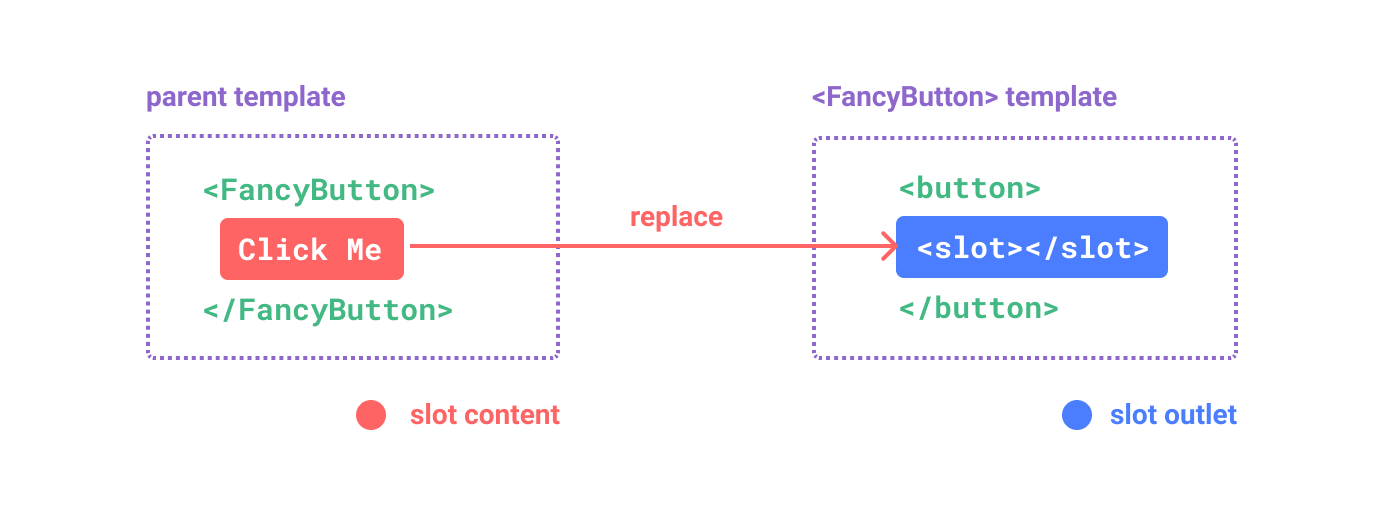
\includegraphics{./img/slots.dbdaf1e8.png} 
\end{center}


\columnratio{0.55}
\begin{paracol}{2}
\switchcolumn[0]*%%%%%%%
And the final rendered DOM:
\switchcolumn
最终渲染出的 DOM 是这样:
\switchcolumn[0]*%%%%%%%
\begin{codeHtml}
<button class="fancy-btn">Click me!</button>
\end{codeHtml}
\switchcolumn
\begin{codeHtml}
<button class="fancy-btn">Click me!</button>
\end{codeHtml}
\switchcolumn[0]*%%%%%%%
\href{https://play.vuejs.org/\#eNpdUdlqAyEU/ZVbQ0kLMdNsXabTQFvoV8yLcRkkjopLSQj596oTwqRvnuM9y9UT+rR2/hs5qlHjqZM2gOch2m2rZW+NC/BDND1+xRCMBuFMD9N5NeKyeNrqphrUSZdA4L1VJPCEAJrRdCEAvpWke+g5NHcYg1cmADU6cB0A4zzThmYckqimupqiGfpXILe/zdwNhaki3n+0SOR5vAu6ReU++efUajtqYGJQ/FIg5w8Wt9FlOx+OKh/nV1c4ZVNqlHE1TIQQ7xnvCN13zkTNalBSc+Jw5wiTac2H1WLDeDeDyXrJVm9LWG7uE3hev3AhHge1cYwnO200L4QljEnd1bCxB1g82UNhe+I6qQs5kuGcE30NrxeaRudzOWtkemeXuHP5tLIKOv8BN+mw3w==}{Try
it in the Playground}
\switchcolumn
\href{https://play.vuejs.org/\#eNpdUdlqAyEU/ZVbQ0kLMdNsXabTQFvoV8yLcRkkjopLSQj596oTwqRvnuM9y9UT+rR2/hs5qlHjqZM2gOch2m2rZW+NC/BDND1+xRCMBuFMD9N5NeKyeNrqphrUSZdA4L1VJPCEAJrRdCEAvpWke+g5NHcYg1cmADU6cB0A4zzThmYckqimupqiGfpXILe/zdwNhaki3n+0SOR5vAu6ReU++efUajtqYGJQ/FIg5w8Wt9FlOx+OKh/nV1c4ZVNqlHE1TIQQ7xnvCN13zkTNalBSc+Jw5wiTac2H1WLDeDeDyXrJVm9LWG7uE3hev3AhHge1cYwnO200L4QljEnd1bCxB1g82UNhe+I6qQs5kuGcE30NrxeaRudzOWtkemeXuHP5tLIKOv8BN+mw3w==}{在演练场中尝试一下}

\switchcolumn[0]*%%%%%%%
With slots, the \texttt{\textless{}FancyButton\textgreater{}} is
responsible for rendering the outer
\texttt{\textless{}button\textgreater{}} (and its fancy styling), while
the inner content is provided by the parent component.
\switchcolumn
通过使用插槽,\texttt{\textless{}FancyButton\textgreater{}}
仅负责渲染外层的 \texttt{\textless{}button\textgreater{}}
(以及相应的样式),而其内部的内容由父组件提供。
\switchcolumn[0]*%%%%%%%
Another way to understand slots is by comparing them to JavaScript
functions:
\switchcolumn
理解插槽的另一种方式是和下面的 JavaScript 函数作类比,其概念是类似的:
\switchcolumn[0]*%%%%%%%
\begin{codeJs}
// 父元素传入插槽内容
FancyButton('Click me!')
// FancyButton 在自己的模板中渲染插槽内容
function FancyButton(slotContent) {
  return `<button class="fancy-btn">
      ${slotContent}
    </button>`
}
\end{codeJs}
\switchcolumn
\begin{codeJs}
// 父元素传入插槽内容
FancyButton('Click me!')
// FancyButton 在自己的模板中渲染插槽内容
function FancyButton(slotContent) {
  return `<button class="fancy-btn">
      ${slotContent}
    </button>`
}
\end{codeJs}
\switchcolumn[0]*%%%%%%%
Slot content is not just limited to text. It can be any valid template
content. For example, we can pass in multiple elements, or even other
components:
\switchcolumn
插槽内容可以是任意合法的模板内容,不局限于文本。例如我们可以传入多个元素,甚至是组件:
\switchcolumn[0]*%%%%%%%
\begin{codeHtml}
<FancyButton>
  <span style="color:red">Click me!</span>
  <AwesomeIcon name="plus" />
</FancyButton>
\end{codeHtml}
\switchcolumn
\begin{codeHtml}
<FancyButton>
  <span style="color:red">Click me!</span>
  <AwesomeIcon name="plus" />
</FancyButton>
\end{codeHtml}
\switchcolumn[0]*%%%%%%%
\href{https://play.vuejs.org/\#eNp1UmtOwkAQvspQYtCEgrx81EqCJibeoX+W7bRZaHc3+1AI4QyewH8ewvN4Aa/gbgtNIfFf5+vMfI/ZXbCQcvBmMYiCWFPFpAGNxsp5wlkphTLwQjjdPlljBIdMiRJ6g2EL88O9pnnxjlqU+EpbzS3s0BwPaypH4gqDpSyIQVcBxK3VFQDwXDC6hhJdlZi4zf3fRKwl4aDNtsDHJKCiECqiW8KTYH5c1gEnwnUdJ9rCh/XeM6Z42AgN+sFZAj6+Ux/LOjFaEK2diMz3h0vjNfj/zokuhPFU3lTdfcpShVOZcJ+DZgHs/HxtCrpZlj34eknoOlfC8jSCgnEkKswVSRlyczkZzVLM+9CdjtPJ/RjGswtX3ExvMcuu6mmhUnTruOBYAZKkKeN5BDO5gdG13FRoSVTOeAW2xkLPY3UEdweYWqW9OCkYN6gctq9uXllx2Z09CJ9dJwzBascI7nBYihWDldUGMqEgdTVIq6TQqCEMfUpNSD+fX7/fH+3b7P8AdGP6wA==}{Try
it in the Playground}
\switchcolumn
\href{https://play.vuejs.org/\#eNp1UmtOwkAQvspQYtCEgrx81EqCJibeoX+W7bRZaHc3+1AI4QyewH8ewvN4Aa/gbgtNIfFf5+vMfI/ZXbCQcvBmMYiCWFPFpAGNxsp5wlkphTLwQjjdPlljBIdMiRJ6g2EL88O9pnnxjlqU+EpbzS3s0BwPaypH4gqDpSyIQVcBxK3VFQDwXDC6hhJdlZi4zf3fRKwl4aDNtsDHJKCiECqiW8KTYH5c1gEnwnUdJ9rCh/XeM6Z42AgN+sFZAj6+Ux/LOjFaEK2diMz3h0vjNfj/zokuhPFU3lTdfcpShVOZcJ+DZgHs/HxtCrpZlj34eknoOlfC8jSCgnEkKswVSRlyczkZzVLM+9CdjtPJ/RjGswtX3ExvMcuu6mmhUnTruOBYAZKkKeN5BDO5gdG13FRoSVTOeAW2xkLPY3UEdweYWqW9OCkYN6gctq9uXllx2Z09CJ9dJwzBascI7nBYihWDldUGMqEgdTVIq6TQqCEMfUpNSD+fX7/fH+3b7P8AdGP6wA==}{在演练场中尝试一下}
\switchcolumn[0]*%%%%%%%
By using slots, our \texttt{\textless{}FancyButton\textgreater{}} is
more flexible and reusable. We can now use it in different places with
different inner content, but all with the same fancy styling.
\switchcolumn
通过使用插槽,\texttt{\textless{}FancyButton\textgreater{}}
组件更加灵活和具有可复用性。现在组件可以用在不同的地方渲染各异的内容,但同时还保证都具有相同的样式。
\switchcolumn[0]*%%%%%%%
Vue components' slot mechanism is inspired by the
\href{https://developer.mozilla.org/en-US/docs/Web/HTML/Element/slot}{native
Web Component `` element}, but with additional capabilities that we will
see later.
\switchcolumn
Vue
组件的插槽机制是受\href{https://developer.mozilla.org/en-US/docs/Web/HTML/Element/slot}{原生
Web Component ``
元素}的启发而诞生,同时还做了一些功能拓展,这些拓展的功能我们后面会学习到。
\end{paracol}


\columnratio{0.55}
\begin{paracol}{2}
\switchcolumn[0]*%%%%%%%
\subsection{Render Scope}
\switchcolumn
\subsection{渲染作用域}
\switchcolumn[0]*%%%%%%%
Slot content has access to the data scope of the parent component,
because it is defined in the parent. For example:
\switchcolumn
插槽内容可以访问到父组件的数据作用域,因为插槽内容本身是在父组件模板中定义的。举例来说:
\switchcolumn[0]*%%%%%%%
\begin{codeHtml}
<span>{{ message }}</span>
<FancyButton>{{ message }}</FancyButton>
\end{codeHtml}
\switchcolumn
\begin{codeHtml}
<span>{{ message }}</span>
<FancyButton>{{ message }}</FancyButton>
\end{codeHtml}
\switchcolumn[0]*%%%%%%%
Here both \texttt{\{\{\ message\ \}\}} interpolations will render the
same content.
\switchcolumn
这里的两个 \texttt{\{\{\ message\ \}\}} 插值表达式渲染的内容都是一样的。
\switchcolumn[0]*%%%%%%%
Slot content does \textbf{not} have access to the child component's
data. Expressions in Vue templates can only access the scope it is
defined in, consistent with JavaScript's lexical scoping. In other
words:
\switchcolumn
插槽内容\textbf{无法访问}子组件的数据。Vue
模板中的表达式只能访问其定义时所处的作用域,这和 JavaScript
的词法作用域规则是一致的。换言之:
\switchcolumn[0]*%%%%%%%
\begin{quote}
Expressions in the parent template only have access to the parent scope;
expressions in the child template only have access to the child scope.
\end{quote}
\switchcolumn
\begin{quote}
父组件模板中的表达式只能访问父组件的作用域;子组件模板中的表达式只能访问子组件的作用域。
\end{quote}
\end{paracol}


\columnratio{0.55}
\begin{paracol}{2}

\switchcolumn[0]*%%%%%%%
\subsection{Fallback Content}
\switchcolumn
\subsection{默认内容}
\switchcolumn[0]*%%%%%%%
There are cases when it's useful to specify fallback (i.e. default)
content for a slot, to be rendered only when no content is provided. For
example, in a \texttt{\textless{}SubmitButton\textgreater{}} component:
\switchcolumn
在外部没有提供任何内容的情况下,可以为插槽指定默认内容。比如有这样一个
\texttt{\textless{}SubmitButton\textgreater{}} 组件:
\switchcolumn[0]*%%%%%%%
\begin{codeHtml}
<button type="submit">
    <slot></slot>
</button>
\end{codeHtml}
\switchcolumn
\begin{codeHtml}
<button type="submit">
    <slot></slot>
</button>
\end{codeHtml}
\switchcolumn[0]*%%%%%%%
We might want the text "Submit" to be rendered inside the
\texttt{\textless{}button\textgreater{}} if the parent didn't provide
any slot content. To make "Submit" the fallback content, we can place it
in between the \texttt{\textless{}slot\textgreater{}} tags:
\switchcolumn
如果我们想在父组件没有提供任何插槽内容时在
\texttt{\textless{}button\textgreater{}}
内渲染``Submit'',只需要将``Submit''写在
\texttt{\textless{}slot\textgreater{}} 标签之间来作为默认内容:
\switchcolumn[0]*%%%%%%%
\begin{codeHtml}
<button type="submit">
    <slot>
    Submit <!-- 默认内容 -->
    </slot>
</button>
\end{codeHtml}
\switchcolumn
\begin{codeHtml}
<button type="submit">
    <slot>
    Submit <!-- 默认内容 -->
    </slot>
</button>
\end{codeHtml}
\switchcolumn[0]*%%%%%%%
Now when we use \texttt{\textless{}SubmitButton\textgreater{}} in a
parent component, providing no content for the slot:
\switchcolumn
现在,当我们在父组件中使用
\texttt{\textless{}SubmitButton\textgreater{}}
且没有提供任何插槽内容时:
\switchcolumn[0]*%%%%%%%
\begin{codeHtml}
<SubmitButton />
\end{codeHtml}
\switchcolumn
\begin{codeHtml}
<SubmitButton />
\end{codeHtml}
\switchcolumn[0]*%%%%%%%
This will render the fallback content, "Submit":
\switchcolumn
``Submit''将会被作为默认内容渲染:
\switchcolumn[0]*%%%%%%%
\begin{codeHtml}
<button type="submit">Submit</button>
\end{codeHtml}
\switchcolumn
\begin{codeHtml}
<button type="submit">Submit</button>
\end{codeHtml}
\switchcolumn[0]*%%%%%%%
But if we provide content:
\switchcolumn
但如果我们提供了插槽内容:
\switchcolumn[0]*%%%%%%%
\begin{codeHtml}
<SubmitButton>Save</SubmitButton>
\end{codeHtml}
\switchcolumn
\begin{codeHtml}
<SubmitButton>Save</SubmitButton>
\end{codeHtml}
\switchcolumn[0]*%%%%%%%
Then the provided content will be rendered instead:
\switchcolumn
那么被显式提供的内容会取代默认内容:
\switchcolumn[0]*%%%%%%%
\begin{codeHtml}
<button type="submit">Save</button>
\end{codeHtml}
\switchcolumn
\begin{codeHtml}
<button type="submit">Save</button>
\end{codeHtml}
\switchcolumn[0]*%%%%%%%
\href{https://play.vuejs.org/\#eNp1kMsKwjAQRX9lzMaNbfcSC/oL3WbT1ikU8yKZFEX8d5MGgi2YVeZxZ86dN7taWy8B2ZlxP7rZEnikYFuhZ2WNI+jCoGa6BSKjYXJGwbFufpNJfhSaN1kflTEgVFb2hDEC4IeqguARpl7KoR8fQPgkqKpc3Wxo1lxRWWeW+Y4wBk9x9V9d2/UL8g1XbOJN4WAntodOnrecQ2agl8WLYH7tFyw5olj10iR3EJ+gPCxDFluj0YS6EAqKR8mi9M3Td1ifLxWShcU=}{Try
it in the Playground}
\switchcolumn
\href{https://play.vuejs.org/\#eNp1kMsKwjAQRX9lzMaNbfcSC/oL3WbT1ikU8yKZFEX8d5MGgi2YVeZxZ86dN7taWy8B2ZlxP7rZEnikYFuhZ2WNI+jCoGa6BSKjYXJGwbFufpNJfhSaN1kflTEgVFb2hDEC4IeqguARpl7KoR8fQPgkqKpc3Wxo1lxRWWeW+Y4wBk9x9V9d2/UL8g1XbOJN4WAntodOnrecQ2agl8WLYH7tFyw5olj10iR3EJ+gPCxDFluj0YS6EAqKR8mi9M3Td1ifLxWShcU=}{在演练场中尝试一下}
\end{paracol}

\columnratio{0.55}
\begin{paracol}{2}

\switchcolumn[0]*%%%%%%%
\subsection{Named Slots}
\switchcolumn
\subsection{具名插槽}
\switchcolumn[0]*%%%%%%%
There are times when it's useful to have multiple slot outlets in a
single component. For example, in a
\texttt{\textless{}BaseLayout\textgreater{}} component with the
following template:
\switchcolumn
有时在一个组件中包含多个插槽出口是很有用的。举例来说,在一个
\texttt{\textless{}BaseLayout\textgreater{}} 组件中,有如下模板:
\switchcolumn[0]*%%%%%%%
\begin{codeHtml}
<div class="container">
    <header>
    <!-- 标题内容放这里 -->
    </header>
    <main>
    <!-- 主要内容放这里 -->
    </main>
    <footer>
    <!-- 底部内容放这里 -->
    </footer>
</div>
\end{codeHtml}
\switchcolumn
\begin{codeHtml}
<div class="container">
    <header>
    <!-- 标题内容放这里 -->
    </header>
    <main>
    <!-- 主要内容放这里 -->
    </main>
    <footer>
    <!-- 底部内容放这里 -->
    </footer>
</div>
\end{codeHtml}
\switchcolumn[0]*%%%%%%%
For these cases, the \texttt{\textless{}slot\textgreater{}} element has
a special attribute, \texttt{name}, which can be used to assign a unique
ID to different slots so you can determine where content should be
rendered:
\switchcolumn
对于这种场景,\texttt{\textless{}slot\textgreater{}}
元素可以有一个特殊的 attribute \texttt{name},用来给各个插槽分配唯一的
ID,以确定每一处要渲染的内容:
\switchcolumn[0]*%%%%%%%
\begin{codeHtml}
<div class="container">
    <header>
    <slot name="header"></slot>
    </header>
    <main>
    <slot></slot>
    </main>
    <footer>
    <slot name="footer"></slot>
    </footer>
</div>
\end{codeHtml}
\switchcolumn
\begin{codeHtml}
<div class="container">
    <header>
    <slot name="header"></slot>
    </header>
    <main>
    <slot></slot>
    </main>
    <footer>
    <slot name="footer"></slot>
    </footer>
</div>
\end{codeHtml}
\switchcolumn[0]*%%%%%%%
A \texttt{\textless{}slot\textgreater{}} outlet without \texttt{name}
implicitly has the name "default".
\switchcolumn
这类带 \texttt{name} 的插槽被称为具名插槽 (named slots)。没有提供
\texttt{name} 的 \texttt{\textless{}slot\textgreater{}}
出口会隐式地命名为``default''。
\switchcolumn[0]*%%%%%%%
In a parent component using
\texttt{\textless{}BaseLayout\textgreater{}}, we need a way to pass
multiple slot content fragments, each targeting a different slot outlet.
This is where \textbf{named slots} come in.
\switchcolumn
在父组件中使用 \texttt{\textless{}BaseLayout\textgreater{}}
时,我们需要一种方式将多个插槽内容传入到各自目标插槽的出口。此时就需要用到\textbf{具名插槽}了:
\switchcolumn[0]*%%%%%%%
To pass a named slot, we need to use a
\texttt{\textless{}template\textgreater{}} element with the
\texttt{v-slot} directive, and then pass the name of the slot as an
argument to \texttt{v-slot}:
\switchcolumn
要为具名插槽传入内容,我们需要使用一个含 \texttt{v-slot} 指令的
\texttt{\textless{}template\textgreater{}}
元素,并将目标插槽的名字传给该指令:
\switchcolumn[0]*%%%%%%%
\begin{codeHtml}
<BaseLayout>
  <template v-slot:header>
    <!-- header 插槽的内容放这里 -->
  </template>
</BaseLayout>
\end{codeHtml}
\switchcolumn
\begin{codeHtml}
<BaseLayout>
  <template v-slot:header>
    <!-- header 插槽的内容放这里 -->
  </template>
</BaseLayout>
\end{codeHtml}
\switchcolumn[0]*%%%%%%%
\texttt{v-slot} has a dedicated shorthand \texttt{\#}, so
\texttt{\textless{}template\ v-slot:header\textgreater{}} can be
shortened to just \texttt{\textless{}template\ \#header\textgreater{}}.
Think of it as "render this template fragment in the child component's
'header' slot".
\switchcolumn
\texttt{v-slot} 有对应的简写 \texttt{\#},因此
\texttt{\textless{}template\ v-slot:header\textgreater{}} 可以简写为
\texttt{\textless{}template\ \#header\textgreater{}}。其意思就是``将这部分模板片段传入子组件的
header 插槽中''。
\end{paracol}

\begin{center} 
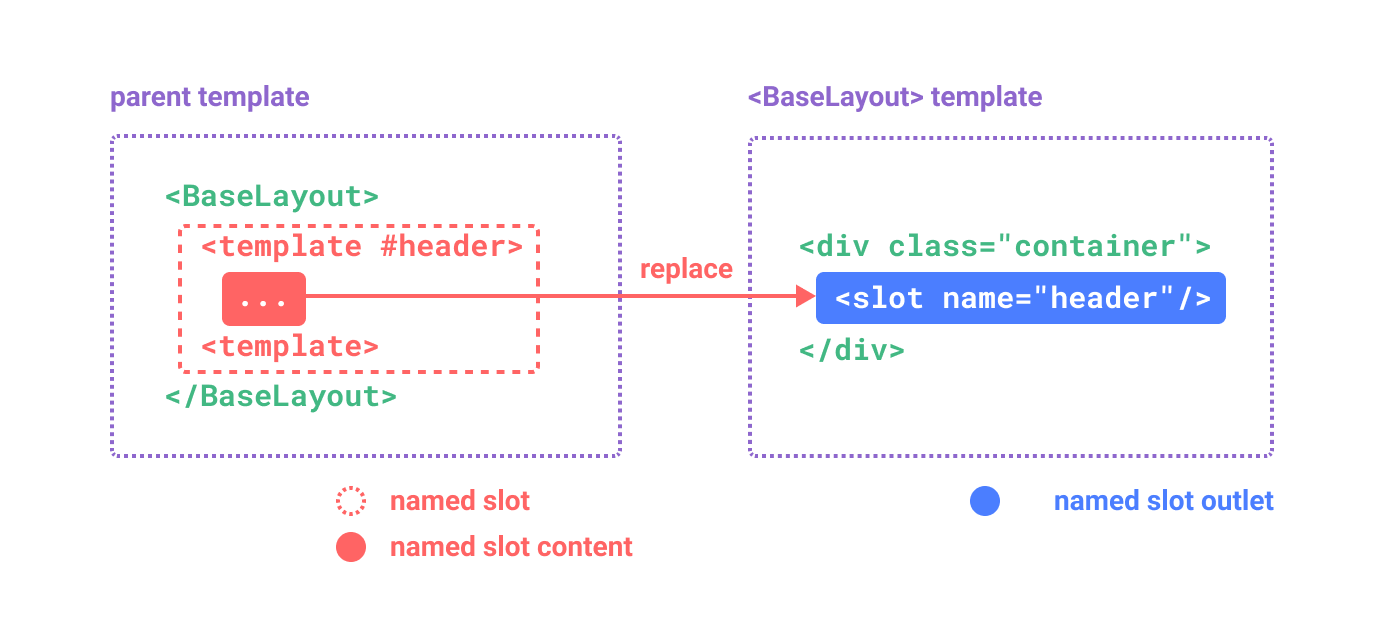
\includegraphics{./img/named-slots.ebb7b207.png} 
\end{center}


\columnratio{0.55}
\begin{paracol}{2}

\switchcolumn[0]*%%%%%%%
Here's the code passing content for all three slots to
\texttt{\textless{}BaseLayout\textgreater{}} using the shorthand syntax:
\switchcolumn
下面我们给出完整的、向 \texttt{\textless{}BaseLayout\textgreater{}}
传递插槽内容的代码,指令均使用的是缩写形式:
\switchcolumn[0]*%%%%%%%
\begin{codeHtml}
<BaseLayout>
    <template #header>
    <h1>Here might be a page title</h1>
    </template>
    <template #default>
    <p>A paragraph for the main content.</p>
    <p>And another one.</p>
    </template>
    <template #footer>
    <p>Here's some contact info</p>
    </template>
</BaseLayout>
\end{codeHtml}
\switchcolumn
\begin{codeHtml}
<BaseLayout>
    <template #header>
    <h1>Here might be a page title</h1>
    </template>
    <template #default>
    <p>A paragraph for the main content.</p>
    <p>And another one.</p>
    </template>
    <template #footer>
    <p>Here's some contact info</p>
    </template>
</BaseLayout>
\end{codeHtml}
\switchcolumn[0]*%%%%%%%
When a component accepts both a default slot and named slots, all
top-level non-\texttt{\textless{}template\textgreater{}} nodes are
implicitly treated as content for the default slot. So the above can
also be written as:
\switchcolumn
当一个组件同时接收默认插槽和具名插槽时,所有位于顶级的非
\texttt{\textless{}template\textgreater{}}
节点都被隐式地视为默认插槽的内容。所以上面也可以写成:
\switchcolumn[0]*%%%%%%%
\begin{codeHtml}
<BaseLayout>
  <template #header>
    <h1>Here might be a page title</h1>
  </template>
  <!-- 隐式的默认插槽 -->
  <p>A paragraph for the main content.</p>
  <p>And another one.</p>
  <template #footer>
    <p>Here's some contact info</p>
  </template>
</BaseLayout>
\end{codeHtml}
\switchcolumn
\begin{codeHtml}
<BaseLayout>
  <template #header>
    <h1>Here might be a page title</h1>
  </template>
  <!-- 隐式的默认插槽 -->
  <p>A paragraph for the main content.</p>
  <p>And another one.</p>
  <template #footer>
    <p>Here's some contact info</p>
  </template>
</BaseLayout>
\end{codeHtml}
\switchcolumn[0]*%%%%%%%
Now everything inside the \texttt{\textless{}template\textgreater{}}
elements will be passed to the corresponding slots. The final rendered
HTML will be:
\switchcolumn
现在 \texttt{\textless{}template\textgreater{}}
元素中的所有内容都将被传递到相应的插槽。最终渲染出的 HTML 如下:
\switchcolumn[0]*%%%%%%%
\begin{codeHtml}
<div class="container">
  <header>
    <h1>Here might be a page title</h1>
  </header>
  <main>
    <p>A paragraph for the main content.</p>
    <p>And another one.</p>
  </main>
  <footer>
    <p>Here's some contact info</p>
  </footer>
</div>
\end{codeHtml}
\switchcolumn
\begin{codeHtml}
<div class="container">
  <header>
    <h1>Here might be a page title</h1>
  </header>
  <main>
    <p>A paragraph for the main content.</p>
    <p>And another one.</p>
  </main>
  <footer>
    <p>Here's some contact info</p>
  </footer>
</div>
\end{codeHtml}
\switchcolumn[0]*%%%%%%%
\href{https://play.vuejs.org/\#eNp9UsFuwjAM/RWrHLgMOi5o6jIkdtphn9BLSF0aKU2ixEVjiH+fm8JoQdvRfu/5xS8+ZVvvl4cOsyITUQXtCSJS5zel1a13geBdRvyUR9cR1MG1MF/mt1YvnZdW5IOWVVwQtt5IQq4AxI2cau5ccZg1KCsMlz4jzWrzgQGh1fuGYIcgwcs9AmkyKHKGLyPykcfD1Apr2ZmrHUN+s+U5Qe6D9A3ULgA1bCK1BeUsoaWlyPuVb3xbgbSOaQGcxRH8v3XtHI0X8mmfeYToWkxmUhFoW7s/JvblJLERmj1l0+T7T5tqK30AZWSMb2WW3LTFUGZXp/u8o3EEVrbI9AFjLn8mt38fN9GIPrSp/p4/Yoj7OMZ+A/boN9KInPeZZpAOLNLRDAsPZDgN4p0L/NQFOV/Ayn9x6EZXMFNKvQ4E5YwLBczW6/WlU3NIi6i/sYDn5Qu2qX1OF51MsvMPkrIEHg==}{Try
it in the Playground}
\switchcolumn
\href{https://play.vuejs.org/\#eNp9UsFuwjAM/RWrHLgMOi5o6jIkdtphn9BLSF0aKU2ixEVjiH+fm8JoQdvRfu/5xS8+ZVvvl4cOsyITUQXtCSJS5zel1a13geBdRvyUR9cR1MG1MF/mt1YvnZdW5IOWVVwQtt5IQq4AxI2cau5ccZg1KCsMlz4jzWrzgQGh1fuGYIcgwcs9AmkyKHKGLyPykcfD1Apr2ZmrHUN+s+U5Qe6D9A3ULgA1bCK1BeUsoaWlyPuVb3xbgbSOaQGcxRH8v3XtHI0X8mmfeYToWkxmUhFoW7s/JvblJLERmj1l0+T7T5tqK30AZWSMb2WW3LTFUGZXp/u8o3EEVrbI9AFjLn8mt38fN9GIPrSp/p4/Yoj7OMZ+A/boN9KInPeZZpAOLNLRDAsPZDgN4p0L/NQFOV/Ayn9x6EZXMFNKvQ4E5YwLBczW6/WlU3NIi6i/sYDn5Qu2qX1OF51MsvMPkrIEHg==}{在演练场中尝试一下}
\switchcolumn[0]*%%%%%%%
Again, it may help you understand named slots better using the
JavaScript function analogy:
\switchcolumn
使用 JavaScript 函数来类比可能更有助于你来理解具名插槽:
\switchcolumn[0]*%%%%%%%
\begin{codeJs}
// 传入不同的内容给不同名字的插槽
BaseLayout({
  header: `...`,
  default: `...`,
  footer: `...`
})
// <BaseLayout> 渲染插槽内容到对应位置
function BaseLayout(slots) {
  return `<div class="container">
      <header>${slots.header}</header>
      <main>${slots.default}</main>
      <footer>${slots.footer}</footer>
    </div>`
}
\end{codeJs}
\switchcolumn
\begin{codeJs}
// 传入不同的内容给不同名字的插槽
BaseLayout({
  header: `...`,
  default: `...`,
  footer: `...`
})
// <BaseLayout> 渲染插槽内容到对应位置
function BaseLayout(slots) {
  return `<div class="container">
      <header>${slots.header}</header>
      <main>${slots.default}</main>
      <footer>${slots.footer}</footer>
    </div>`
}
\end{codeJs}
\end{paracol}


\columnratio{0.55}
\begin{paracol}{2}
 
\switchcolumn[0]*%%%%%%%
\subsection{Dynamic Slot Names}
\switchcolumn
\subsection{动态插槽名}
\switchcolumn[0]*%%%%%%%
\href{https://vuejs.org/guide/essentials/template-syntax.html\#dynamic-arguments}{Dynamic
directive arguments} also work on \texttt{v-slot}, allowing the
definition of dynamic slot names:
\switchcolumn
\href{https://cn.vuejs.org/guide/essentials/template-syntax.html\#dynamic-arguments}{动态指令参数}在
\texttt{v-slot} 上也是有效的,即可以定义下面这样的动态插槽名:
\switchcolumn[0]*%%%%%%%
\begin{codeHtml}
<base-layout>
  <template v-slot:[dynamicSlotName]>
    ...
  </template>
  <!-- 缩写为 -->
  <template #[dynamicSlotName]>
    ...
  </template>
</base-layout>
\end{codeHtml}
\switchcolumn
\begin{codeHtml}
<base-layout>
  <template v-slot:[dynamicSlotName]>
    ...
  </template>
  <!-- 缩写为 -->
  <template #[dynamicSlotName]>
    ...
  </template>
</base-layout>
\end{codeHtml}
\switchcolumn[0]*%%%%%%%
Do note the expression is subject to the
\href{https://vuejs.org/guide/essentials/template-syntax.html\#directives}{syntax
constraints} of dynamic directive arguments.
\switchcolumn
注意这里的表达式和动态指令参数受相同的\href{https://cn.vuejs.org/guide/essentials/template-syntax.html\#directives}{语法限制}。
\end{paracol}

\columnratio{0.55}
\begin{paracol}{2}
\switchcolumn[0]*%%%%%%%
\subsection{Scoped Slots}
\switchcolumn
\subsection{作用域插槽}
\switchcolumn[0]*%%%%%%%
As discussed in
\href{https://vuejs.org/guide/components/slots.html\#render-scope}{Render
Scope}, slot content does not have access to state in the child
component.
\switchcolumn
在上面的\href{https://cn.vuejs.org/guide/components/slots.html\#render-scope}{渲染作用域}中我们讨论到,插槽的内容无法访问到子组件的状态。
\switchcolumn[0]*%%%%%%%
However, there are cases where it could be useful if a slot's content
can make use of data from both the parent scope and the child scope. To
achieve that, we need a way for the child to pass data to a slot when
rendering it.
\switchcolumn
然而在某些场景下插槽的内容可能想要同时使用父组件域内和子组件域内的数据。要做到这一点,我们需要一种方法来让子组件在渲染时将一部分数据提供给插槽。
\switchcolumn[0]*%%%%%%%
In fact, we can do exactly that - we can pass attributes to a slot
outlet just like passing props to a component:
\switchcolumn
我们也确实有办法这么做!可以像对组件传递 props
那样,向一个插槽的出口上传递 attributes:
\switchcolumn[0]*%%%%%%%
\begin{codeHtml}
<!-- <MyComponent> 的模板 -->
<div>
  <slot :text="greetingMessage" :count="1"></slot>
</div>
\end{codeHtml}
\switchcolumn
\begin{codeHtml}
<!-- <MyComponent> 的模板 -->
<div>
  <slot :text="greetingMessage" :count="1"></slot>
</div>
\end{codeHtml}
\switchcolumn[0]*%%%%%%%
Receiving the slot props is a bit different when using a single default
slot vs. using named slots. We are going to show how to receive props
using a single default slot first, by using \texttt{v-slot} directly on
the child component tag:
\switchcolumn
当需要接收插槽 props
时,默认插槽和具名插槽的使用方式有一些小区别。下面我们将先展示默认插槽如何接受
props,通过子组件标签上的 \texttt{v-slot} 指令,直接接收到了一个插槽
props 对象:
\switchcolumn[0]*%%%%%%%
\begin{codeHtml}
<MyComponent v-slot="slotProps">
  {{ slotProps.text }} {{ slotProps.count }}
</MyComponent>
\end{codeHtml}
\switchcolumn
\begin{codeHtml}
<MyComponent v-slot="slotProps">
  {{ slotProps.text }} {{ slotProps.count }}
</MyComponent>
\end{codeHtml}
\end{paracol}

\begin{center} 
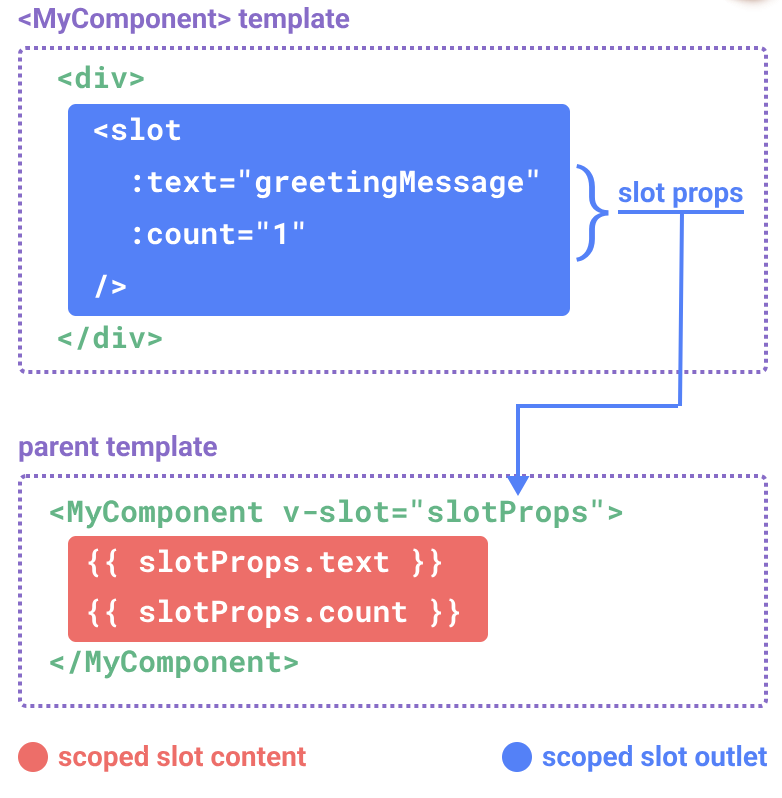
\includegraphics{./img/scoped-slots.1c6d5876.png} 
\end{center}
    


\columnratio{0.55}
\begin{paracol}{2}
 
\switchcolumn[0]*%%%%%%%
\href{https://play.vuejs.org/\#eNp9kMEKgzAMhl8l9OJlU3aVOhg7C3uAXsRlTtC2tFE2pO++dA5xMnZqk+b/8/2dxMnadBxQ5EL62rWWwCMN9qh021vjCMrn2fBNoya4OdNDkmarXhQnSstsVrOOC8LedhVhrEiuHca97wwVSsTj4oz1SvAUgKJpgqWZEj4IQoCvZm0Gtgghzss1BDvIbFkqdmID+CNdbbQnaBwitbop0fuqQSgguWPXmX+JePe1HT/QMtJBHnE51MZOCcjfzPx04JxsydPzp2Szxxo7vABY1I/p}{Try
it in the Playground}
\switchcolumn
\href{https://play.vuejs.org/\#eNp9kMEKgzAMhl8l9OJlU3aVOhg7C3uAXsRlTtC2tFE2pO++dA5xMnZqk+b/8/2dxMnadBxQ5EL62rWWwCMN9qh021vjCMrn2fBNoya4OdNDkmarXhQnSstsVrOOC8LedhVhrEiuHca97wwVSsTj4oz1SvAUgKJpgqWZEj4IQoCvZm0Gtgghzss1BDvIbFkqdmID+CNdbbQnaBwitbop0fuqQSgguWPXmX+JePe1HT/QMtJBHnE51MZOCcjfzPx04JxsydPzp2Szxxo7vABY1I/p}{在演练场中尝试一下}
\switchcolumn[0]*%%%%%%%
The props passed to the slot by the child are available as the value of
the corresponding \texttt{v-slot} directive, which can be accessed by
expressions inside the slot.
\switchcolumn
子组件传入插槽的 props 作为了 \texttt{v-slot}
指令的值,可以在插槽内的表达式中访问。
\switchcolumn[0]*%%%%%%%
You can think of a scoped slot as a function being passed into the child
component. The child component then calls it, passing props as
arguments:
\switchcolumn
你可以将作用域插槽类比为一个传入子组件的函数。子组件会将相应的 props
作为参数传给它:
\switchcolumn[0]*%%%%%%%
\begin{codeJs}
MyComponent({
  // 类比默认插槽,将其想成一个函数
  default: (slotProps) => {
    return `${slotProps.text} ${slotProps.count}`
  }
})
function MyComponent(slots) {
  const greetingMessage = 'hello'
  return `<div>${
    // 在插槽函数调用时传入 props
    slots.default({ text: greetingMessage, count: 1 })
  }</div>`
}
\end{codeJs}
\switchcolumn
\begin{codeJs}
MyComponent({
  // 类比默认插槽,将其想成一个函数
  default: (slotProps) => {
    return `${slotProps.text} ${slotProps.count}`
  }
})
function MyComponent(slots) {
  const greetingMessage = 'hello'
  return `<div>${
    // 在插槽函数调用时传入 props
    slots.default({ text: greetingMessage, count: 1 })
  }</div>`
}
\end{codeJs}
\switchcolumn[0]*%%%%%%%
In fact, this is very close to how scoped slots are compiled, and how
you would use scoped slots in manual
\href{https://vuejs.org/guide/extras/render-function.html}{render
functions}.
\switchcolumn
实际上,这已经和作用域插槽的最终代码编译结果、以及手动编写\href{https://cn.vuejs.org/guide/extras/render-function.html}{渲染函数}时使用作用域插槽的方式非常类似了。
\switchcolumn[0]*%%%%%%%
Notice how \texttt{v-slot="slotProps"} matches the slot function
signature. Just like with function arguments, we can use destructuring
in \texttt{v-slot}:
\switchcolumn
\texttt{v-slot="slotProps"}
可以类比这里的函数签名,和函数的参数类似,我们也可以在 \texttt{v-slot}
中使用解构:
\switchcolumn[0]*%%%%%%%
\begin{codeHtml}
<MyComponent v-slot="{ text, count }">
  {{ text }} {{ count }}
</MyComponent>
\end{codeHtml}
\switchcolumn
\begin{codeHtml}
<MyComponent v-slot="{ text, count }">
  {{ text }} {{ count }}
</MyComponent>
\end{codeHtml} 
\end{paracol}

\columnratio{0.55}
\begin{paracol}{2}
 
\switchcolumn[0]*%%%%%%%
\subsubsection{Named Scoped Slots}
\switchcolumn
\subsubsection{具名作用域插槽}
\switchcolumn[0]*%%%%%%%
Named scoped slots work similarly - slot props are accessible as the
value of the \texttt{v-slot} directive:
\texttt{v-slot:name="slotProps"}. When using the shorthand, it looks
like this:
\switchcolumn
具名作用域插槽的工作方式也是类似的,插槽 props 可以作为 \texttt{v-slot}
指令的值被访问到:\texttt{v-slot:name="slotProps"}。当使用缩写时是这样:
\switchcolumn[0]*%%%%%%%
\begin{codeHtml}
<MyComponent>
  <template #header="headerProps">
    {{ headerProps }}
  </template>
  <template #default="defaultProps">
    {{ defaultProps }}
  </template>
  <template #footer="footerProps">
    {{ footerProps }}
  </template>
</MyComponent>
\end{codeHtml}
\switchcolumn
\begin{codeHtml}
<MyComponent>
  <template #header="headerProps">
    {{ headerProps }}
  </template>
  <template #default="defaultProps">
    {{ defaultProps }}
  </template>
  <template #footer="footerProps">
    {{ footerProps }}
  </template>
</MyComponent>
\end{codeHtml}
\switchcolumn[0]*%%%%%%%
Passing props to a named slot:
\switchcolumn
向具名插槽中传入 props:
\switchcolumn[0]*%%%%%%%
\begin{codeHtml}
<slot name="header" message="hello"></slot>
\end{codeHtml}
\switchcolumn
\begin{codeHtml}
<slot name="header" message="hello"></slot>
\end{codeHtml}
\switchcolumn[0]*%%%%%%%
Note the \texttt{name} of a slot won't be included in the props because
it is reserved - so the resulting \texttt{headerProps} would be
\texttt{\{\ message:\ \textquotesingle{}hello\textquotesingle{}\ \}}.
\switchcolumn
注意插槽上的 \texttt{name} 是一个 Vue 特别保留的 attribute,不会作为
props 传递给插槽。因此最终 \texttt{headerProps} 的结果是
\texttt{\{\ message:\ \textquotesingle{}hello\textquotesingle{}\ \}}。
\switchcolumn[0]*%%%%%%%
If you are mixing named slots with the default scoped slot, you need to
use an explicit \texttt{\textless{}template\textgreater{}} tag for the
default slot. Attempting to place the \texttt{v-slot} directive directly
on the component will result in a compilation error. This is to avoid
any ambiguity about the scope of the props of the default slot. For
example:
\switchcolumn
如果你同时使用了具名插槽与默认插槽,则需要为默认插槽使用显式的
\texttt{\textless{}template\textgreater{}} 标签。尝试直接为组件添加
\texttt{v-slot} 指令将导致编译错误。这是为了避免因默认插槽的 props
的作用域而困惑。举例:
\switchcolumn[0]*%%%%%%%
\begin{codeHtml}
<!-- 该模板无法编译 -->
<template>
  <MyComponent v-slot="{ message }">
    <p>{{ message }}</p>
    <template #footer>
      <!-- message 属于默认插槽,此处不可用 -->
      <p>{{ message }}</p>
    </template>
  </MyComponent>
</template>
\end{codeHtml}
\switchcolumn
\begin{codeHtml}
<!-- 该模板无法编译 -->
<template>
  <MyComponent v-slot="{ message }">
    <p>{{ message }}</p>
    <template #footer>
      <!-- message 属于默认插槽,此处不可用 -->
      <p>{{ message }}</p>
    </template>
  </MyComponent>
</template>
\end{codeHtml}
\switchcolumn[0]*%%%%%%%
Using an explicit \texttt{\textless{}template\textgreater{}} tag for the
default slot helps to make it clear that the \texttt{message} prop is
not available inside the other slot:
\switchcolumn
为默认插槽使用显式的 \texttt{\textless{}template\textgreater{}}
标签有助于更清晰地指出 \texttt{message} 属性在其他插槽中不可用:
\switchcolumn[0]*%%%%%%%
\begin{codeHtml}
<template>
  <MyComponent>
    <!-- 使用显式的默认插槽 -->
    <template #default="{ message }">
      <p>{{ message }}</p>
    </template>
    <template #footer>
      <p>Here's some contact info</p>
    </template>
  </MyComponent>
</template>
\end{codeHtml}
\switchcolumn
\begin{codeHtml}
<template>
  <MyComponent>
    <!-- 使用显式的默认插槽 -->
    <template #default="{ message }">
      <p>{{ message }}</p>
    </template>
    <template #footer>
      <p>Here's some contact info</p>
    </template>
  </MyComponent>
</template>
\end{codeHtml}
\end{paracol}

\columnratio{0.55}
\begin{paracol}{2}
  
\switchcolumn[0]*%%%%%%%
\subsubsection{Fancy List Example}
\switchcolumn
\subsubsection{高级列表组件示例}
\switchcolumn[0]*%%%%%%%
You may be wondering what would be a good use case for scoped slots.
Here's an example: imagine a \texttt{\textless{}FancyList\textgreater{}}
component that renders a list of items - it may encapsulate the logic
for loading remote data, using the data to display a list, or even
advanced features like pagination or infinite scrolling. However, we
want it to be flexible with how each item looks and leave the styling of
each item to the parent component consuming it. So the desired usage may
look like this:
\switchcolumn
你可能想问什么样的场景才适合用到作用域插槽,这里我们来看一个
\texttt{\textless{}FancyList\textgreater{}}
组件的例子。它会渲染一个列表,并同时会封装一些加载远端数据的逻辑、使用数据进行列表渲染、或者是像分页或无限滚动这样更进阶的功能。然而我们希望它能够保留足够的灵活性,将对单个列表元素内容和样式的控制权留给使用它的父组件。我们期望的用法可能是这样的:
\switchcolumn[0]*%%%%%%%
\begin{codeHtml}
<FancyList :api-url="url" :per-page="10">
  <template #item="{ body, username, likes }">
    <div class="item">
      <p>{{ body }}</p>
      <p>by {{ username }} | {{ likes }} likes</p>
    </div>
  </template>
</FancyList>
\end{codeHtml}
\switchcolumn
\begin{codeHtml}
<FancyList :api-url="url" :per-page="10">
  <template #item="{ body, username, likes }">
    <div class="item">
      <p>{{ body }}</p>
      <p>by {{ username }} | {{ likes }} likes</p>
    </div>
  </template>
</FancyList>
\end{codeHtml}
\switchcolumn[0]*%%%%%%%
Inside \texttt{\textless{}FancyList\textgreater{}}, we can render the
same \texttt{\textless{}slot\textgreater{}} multiple times with
different item data (notice we are using \texttt{v-bind} to pass an
object as slot props):
\switchcolumn
在 \texttt{\textless{}FancyList\textgreater{}} 之中,我们可以多次渲染
\texttt{\textless{}slot\textgreater{}} 并每次都提供不同的数据
(注意我们这里使用了 \texttt{v-bind} 来传递插槽的 props):
\switchcolumn[0]*%%%%%%%
\begin{codeHtml}
<ul>
  <li v-for="item in items">
    <slot name="item" v-bind="item"></slot>
  </li>
</ul>
\end{codeHtml}
\switchcolumn
\begin{codeHtml}
<ul>
  <li v-for="item in items">
    <slot name="item" v-bind="item"></slot>
  </li>
</ul>
\end{codeHtml}
\switchcolumn[0]*%%%%%%%
\href{https://play.vuejs.org/\#eNqFU2Fv0zAQ/StHJtROapNuZTBCNwnQQKBpTGxCQss+uMml8+bYlu2UlZL/zjlp0lQa40sU3/nd3Xv3vA7eax0uSwziYGZTw7UDi67Up4nkhVbGwScm09U5tw5yowoYhFEX8cBBImdRgyQMHRwWWjCHdAKYbdFM83FpxEkS0DcJINZoxpotkCIHkySo7xOixcMep19KrmGustUISotGsgJHIPgDWqg6DKEyvoRUMGsJ4HG9HGX16bqpAlU1izy5baqDFegYweYroMttMwLAHx/Y9Kyan36RWUTN2+mjXfpbrei8k6SjdSuBYFOlMaNI6AeAtcflSrqx5b8xhkl4jMU7H0yVUCaGvVeH8+PjKYWqWnpf5DQYBTtb+fc612Awh2qzzGaBiUyVpBVpo7SFE8gw5xIv/Wl4M9gsbjCCQbuywe3+FuXl9iiqO7xpElEEhUofKFQo2mTGiFiOLr3jcpFImuiaF6hKNxzuw8lpw7kuEy6ZKJGK3TR6NluLYXBVqwRXQjkLn0ueIc3TLonyZ0sm4acqKVovKIbDCVQjGsb1qvyg2telU4Yzz6eHv6ARBWdwjVqUNCbbFjqgQn6aW1J8RKfJhDg+5/lStG4QHJZjnpO5XjT0BMqFu+uZ81yxjEQJw7A1kOA76FyZjaWBy0akvu8tCQKeQ+d7wsy5zLpz1FlzU3kW1QP+x40ApWgWAySEJTv6/NitNMkllcTakwCaZZ5ADEf6cROas/RhYVQps5igEpkZLwzRROmG04OjDBcj7+Js+vYQDo9e0uH1qzeY5/s1vtaaqG969+vTTrsmBTMLLv12nuy7l+d5W673SBzxkzlfhPdWSXokdZMkSFWhuUDzTTtOnk6CuG2fBEwI9etrHXOmRLJUE0/vMH14In5vH30sCS4Nkr+WmARdztHQ6Jr02dUFPtJ/lyxUVgq6/UzyO1olSj9jc+0DcaWxe/fqab/UT51Uu7Znjw6lbUn5QWtR6vtJQM//4zPUt+NOw+lGzCqo/gLm1QS8}{Try
it in the Playground}
\switchcolumn
\href{https://play.vuejs.org/\#eNqFU2Fv0zAQ/StHJtROapNuZTBCNwnQQKBpTGxCQss+uMml8+bYlu2UlZL/zjlp0lQa40sU3/nd3Xv3vA7eax0uSwziYGZTw7UDi67Up4nkhVbGwScm09U5tw5yowoYhFEX8cBBImdRgyQMHRwWWjCHdAKYbdFM83FpxEkS0DcJINZoxpotkCIHkySo7xOixcMep19KrmGustUISotGsgJHIPgDWqg6DKEyvoRUMGsJ4HG9HGX16bqpAlU1izy5baqDFegYweYroMttMwLAHx/Y9Kyan36RWUTN2+mjXfpbrei8k6SjdSuBYFOlMaNI6AeAtcflSrqx5b8xhkl4jMU7H0yVUCaGvVeH8+PjKYWqWnpf5DQYBTtb+fc612Awh2qzzGaBiUyVpBVpo7SFE8gw5xIv/Wl4M9gsbjCCQbuywe3+FuXl9iiqO7xpElEEhUofKFQo2mTGiFiOLr3jcpFImuiaF6hKNxzuw8lpw7kuEy6ZKJGK3TR6NluLYXBVqwRXQjkLn0ueIc3TLonyZ0sm4acqKVovKIbDCVQjGsb1qvyg2telU4Yzz6eHv6ARBWdwjVqUNCbbFjqgQn6aW1J8RKfJhDg+5/lStG4QHJZjnpO5XjT0BMqFu+uZ81yxjEQJw7A1kOA76FyZjaWBy0akvu8tCQKeQ+d7wsy5zLpz1FlzU3kW1QP+x40ApWgWAySEJTv6/NitNMkllcTakwCaZZ5ADEf6cROas/RhYVQps5igEpkZLwzRROmG04OjDBcj7+Js+vYQDo9e0uH1qzeY5/s1vtaaqG969+vTTrsmBTMLLv12nuy7l+d5W673SBzxkzlfhPdWSXokdZMkSFWhuUDzTTtOnk6CuG2fBEwI9etrHXOmRLJUE0/vMH14In5vH30sCS4Nkr+WmARdztHQ6Jr02dUFPtJ/lyxUVgq6/UzyO1olSj9jc+0DcaWxe/fqab/UT51Uu7Znjw6lbUn5QWtR6vtJQM//4zPUt+NOw+lGzCqo/gLm1QS8}{在演练场中尝试一下}
\end{paracol}


\columnratio{0.55}
\begin{paracol}{2}
 
\switchcolumn[0]*%%%%%%%
\subsubsection{Renderless Components}
\switchcolumn
\subsubsection{无渲染组件}
\switchcolumn[0]*%%%%%%%
The \texttt{\textless{}FancyList\textgreater{}} use case we discussed
above encapsulates both reusable logic (data fetching, pagination etc.)
and visual output, while delegating part of the visual output to the
consumer component via scoped slots.
\switchcolumn
上面的 \texttt{\textless{}FancyList\textgreater{}}
案例同时封装了可重用的逻辑 (数据获取、分页等)
和视图输出,但也将部分视图输出通过作用域插槽交给了消费者组件来管理。
\switchcolumn[0]*%%%%%%%
If we push this concept a bit further, we can come up with components
that only encapsulate logic and do not render anything by themselves -
visual output is fully delegated to the consumer component with scoped
slots. We call this type of component a \textbf{Renderless Component}.
\switchcolumn
如果我们将这个概念拓展一下,可以想象的是,一些组件可能只包括了逻辑而不需要自己渲染内容,视图输出通过作用域插槽全权交给了消费者组件。我们将这种类型的组件称为\textbf{无渲染组件}。
\switchcolumn[0]*%%%%%%%
An example renderless component could be one that encapsulates the logic
of tracking the current mouse position:
\switchcolumn
这里有一个无渲染组件的例子,一个封装了追踪当前鼠标位置逻辑的组件:
\switchcolumn[0]*%%%%%%%
\begin{codeHtml}
<MouseTracker v-slot="{ x, y }">
  Mouse is at: {{ x }}, {{ y }}
</MouseTracker>
\end{codeHtml}
\switchcolumn
\begin{codeHtml}
<MouseTracker v-slot="{ x, y }">
  Mouse is at: {{ x }}, {{ y }}
</MouseTracker>
\end{codeHtml}
\switchcolumn[0]*%%%%%%%
\href{https://play.vuejs.org/\#eNqNUcFqhDAQ/ZUhF12w2rO4Cz301t5aaCEX0dki1SQko6uI/96J7i4qLPQQmHmZ9+Y9ZhQvxsRdiyIVmStsZQgcUmtOUlWN0ZbgXbcOP2xe/KKFs9UNBHGyBj09kCpLFj4zuSFsTJ0T+o6yjUb35GpNRylG6CMYYJKCpwAkzWNQOcgphZG/YZoiX/DQNAttFjMrS+6LRCT2rh6HGsHiOQKtmKIIS19+qmZpYLrmXIKxM1Vo5Yj9HD0vfD7ckGGF3LDWlOyHP/idYPQCfdzldTtjscl/8MuDww78lsqHVHdTYXjwCpdKlfoS52X52qGit8oRKrRhwHYdNrrDILouPbCNVZCtgJ1n/6Xx8JYAmT8epD3fr5cC0oGLQYpkd4zpD27R0vA=}{Try
it in the Playground}
\switchcolumn
\href{https://play.vuejs.org/\#eNqNUcFqhDAQ/ZUhF12w2rO4Cz301t5aaCEX0dki1SQko6uI/96J7i4qLPQQmHmZ9+Y9ZhQvxsRdiyIVmStsZQgcUmtOUlWN0ZbgXbcOP2xe/KKFs9UNBHGyBj09kCpLFj4zuSFsTJ0T+o6yjUb35GpNRylG6CMYYJKCpwAkzWNQOcgphZG/YZoiX/DQNAttFjMrS+6LRCT2rh6HGsHiOQKtmKIIS19+qmZpYLrmXIKxM1Vo5Yj9HD0vfD7ckGGF3LDWlOyHP/idYPQCfdzldTtjscl/8MuDww78lsqHVHdTYXjwCpdKlfoS52X52qGit8oRKrRhwHYdNrrDILouPbCNVZCtgJ1n/6Xx8JYAmT8epD3fr5cC0oGLQYpkd4zpD27R0vA=}{在演练场中尝试一下}
\switchcolumn[0]*%%%%%%%
While an interesting pattern, most of what can be achieved with
Renderless Components can be achieved in a more efficient fashion with
Composition API, without incurring the overhead of extra component
nesting. Later, we will see how we can implement the same mouse tracking
functionality as a
\href{https://vuejs.org/guide/reusability/composables.html}{Composable}.
\switchcolumn
虽然这个模式很有趣,但大部分能用无渲染组件实现的功能都可以通过组合式 API
以另一种更高效的方式实现,并且还不会带来额外组件嵌套的开销。之后我们会在\href{https://cn.vuejs.org/guide/reusability/composables.html}{组合式函数}一章中介绍如何更高效地实现追踪鼠标位置的功能。
\switchcolumn[0]*%%%%%%%
That said, scoped slots are still useful in cases where we need to both
encapsulate logic \textbf{and} compose visual output, like in the
\texttt{\textless{}FancyList\textgreater{}} example.
\switchcolumn
尽管如此,作用域插槽在需要\textbf{同时}封装逻辑、组合视图界面时还是很有用,就像上面的
\texttt{\textless{}FancyList\textgreater{}} 组件那样。
\end{paracol}



\columnratio{0.55}
\begin{paracol}{2}
 
\end{paracol}

\columnratio{0.55}
\begin{paracol}{2}
\switchcolumn[0]*%%%%%%%
\section{Provide / Inject}
\switchcolumn
\section{依赖注入}
\switchcolumn[0]*%%%%%%%
\begin{quote}
This page assumes you've already read the
\href{https://vuejs.org/guide/essentials/component-basics.html}{Components
Basics}. Read that first if you are new to components.
\end{quote}
\switchcolumn
\begin{quote}
此章节假设你已经看过了\href{https://cn.vuejs.org/guide/essentials/component-basics.html}{组件基础}。若你还不了解组件是什么,请先阅读该章节。
\end{quote}
\switchcolumn[0]*%%%%%%%
\subsection{Prop Drilling}
\switchcolumn
\subsection{Prop 逐级透传问题}
\switchcolumn[0]*%%%%%%%
Usually, when we need to pass data from the parent to a child component,
we use \href{https://vuejs.org/guide/components/props.html}{props}.
However, imagine the case where we have a large component tree, and a
deeply nested component needs something from a distant ancestor
component. With only props, we would have to pass the same prop across
the entire parent chain:
\switchcolumn
通常情况下,当我们需要从父组件向子组件传递数据时,会使用
\href{https://cn.vuejs.org/guide/components/props.html}{props}。想象一下这样的结构:有一些多层级嵌套的组件,形成了一颗巨大的组件树,而某个深层的子组件需要一个较远的祖先组件中的部分数据。在这种情况下,如果仅使用
props 则必须将其沿着组件链逐级传递下去,这会非常麻烦:
\end{paracol}

\begin{center} 
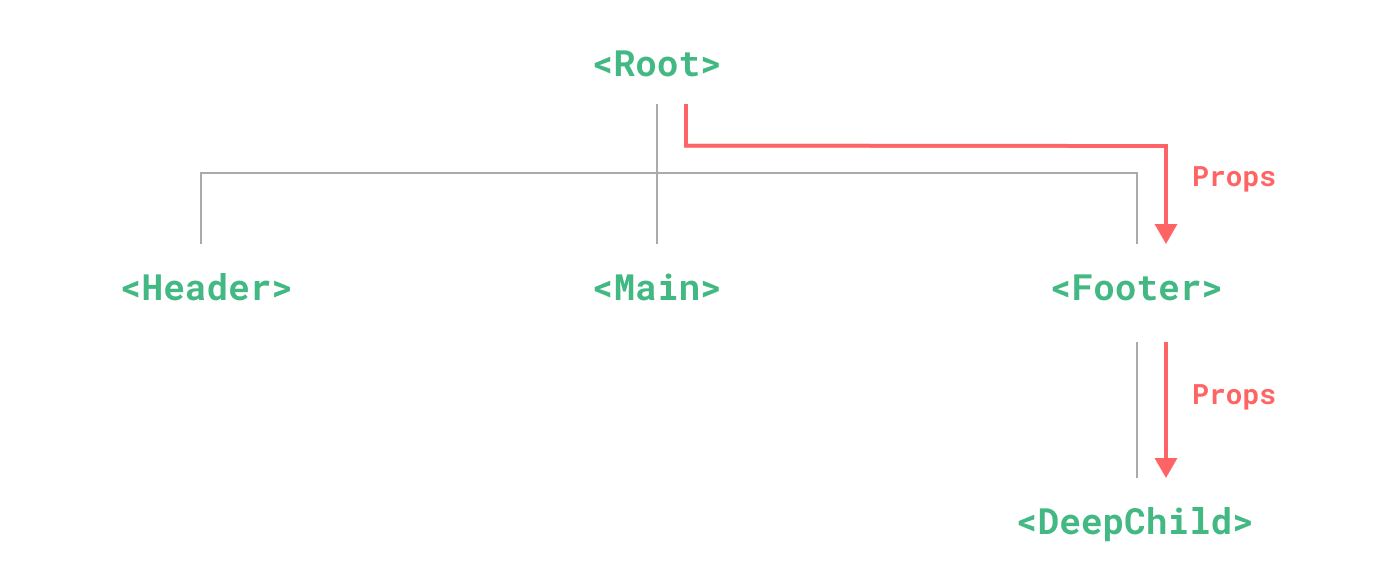
\includegraphics{./img/prop-drilling.11201220.png} 
\end{center}

\columnratio{0.55}
\begin{paracol}{2}
\switchcolumn[0]*%%%%%%%
Notice although the \texttt{\textless{}Footer\textgreater{}} component
may not care about these props at all, it still needs to declare and
pass them along just so \texttt{\textless{}DeepChild\textgreater{}} can
access them. If there is a longer parent chain, more components would be
affected along the way. This is called "props drilling" and definitely
isn't fun to deal with.
\switchcolumn
注意,虽然这里的 \texttt{\textless{}Footer\textgreater{}}
组件可能根本不关心这些 props,但为了使
\texttt{\textless{}DeepChild\textgreater{}}
能访问到它们,仍然需要定义并向下传递。如果组件链路非常长,可能会影响到更多这条路上的组件。这一问题被称为``prop
逐级透传'',显然是我们希望尽量避免的情况。
\switchcolumn[0]*%%%%%%%
We can solve props drilling with \texttt{provide} and \texttt{inject}. A
parent component can serve as a \textbf{dependency provider} for all its
descendants. Any component in the descendant tree, regardless of how
deep it is, can \textbf{inject} dependencies provided by components up
in its parent chain.
\switchcolumn
\texttt{provide} 和 \texttt{inject} 可以帮助我们解决这一问题。
\href{https://cn.vuejs.org/guide/components/provide-inject.html\#footnote-1}{{[}1{]}}
一个父组件相对于其所有的后代组件,会作为\textbf{依赖提供者}。任何后代的组件树,无论层级有多深,都可以\textbf{注入}由父组件提供给整条链路的依赖。
\end{paracol}

\begin{center} 
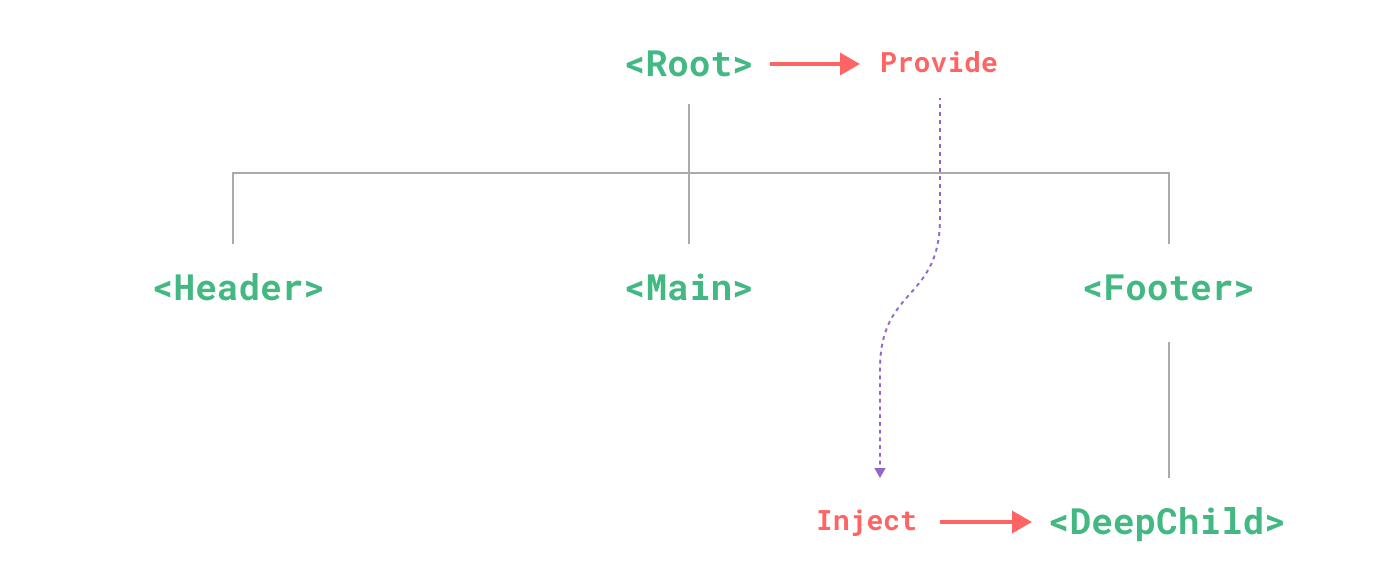
\includegraphics{./img/provide-inject.3e0505e4.png} 
\end{center}

\columnratio{0.55}
\begin{paracol}{2}
 
\switchcolumn[0]*%%%%%%%
\subsection{Provide}
\switchcolumn
\subsection{Provide (提供)}
\switchcolumn[0]*%%%%%%%
To provide data to a component's descendants, use the
\href{https://vuejs.org/api/composition-api-dependency-injection.html\#provide}{\texttt{provide()}}
function:
\switchcolumn
要为组件后代提供数据,需要使用到
\href{https://cn.vuejs.org/api/composition-api-dependency-injection.html\#provide}{\texttt{provide()}}
函数:
\switchcolumn[0]*%%%%%%%
\begin{codeHtml}
<script setup>
import { provide } from 'vue'
provide(/* 注入名 */ 'message', /* 值 */ 'hello!')
</script>
\end{codeHtml}
\switchcolumn
\begin{codeHtml}
<script setup>
import { provide } from 'vue'
provide(/* 注入名 */ 'message', /* 值 */ 'hello!')
</script>
\end{codeHtml}
\switchcolumn[0]*%%%%%%%
If not using \texttt{\textless{}script\ setup\textgreater{}}, make sure
\texttt{provide()} is called synchronously inside \texttt{setup()}:
\switchcolumn
如果不使用 \texttt{\textless{}script\ setup\textgreater{}},请确保
\texttt{provide()} 是在 \texttt{setup()} 同步调用的:
\switchcolumn[0]*%%%%%%%
\begin{codeJs}
import { provide } from 'vue'
export default {
  setup() {
    provide(/* 注入名 */ 'message', /* 值 */ 'hello!')
  }
}
\end{codeJs}
\switchcolumn
\begin{codeJs}
import { provide } from 'vue'
export default {
  setup() {
    provide(/* 注入名 */ 'message', /* 值 */ 'hello!')
  }
}
\end{codeJs}
\switchcolumn[0]*%%%%%%%
The \texttt{provide()} function accepts two arguments. The first
argument is called the \textbf{injection key}, which can be a string or
a \texttt{Symbol}. The injection key is used by descendant components to
lookup the desired value to inject. A single component can call
\texttt{provide()} multiple times with different injection keys to
provide different values.
\switchcolumn
\texttt{provide()}
函数接收两个参数。第一个参数被称为\textbf{注入名},可以是一个字符串或是一个
\texttt{Symbol}。后代组件会用注入名来查找期望注入的值。一个组件可以多次调用
\texttt{provide()},使用不同的注入名,注入不同的依赖值。
\switchcolumn[0]*%%%%%%%
The second argument is the provided value. The value can be of any type,
including reactive state such as refs:
\switchcolumn
第二个参数是提供的值,值可以是任意类型,包括响应式的状态,比如一个 ref:
\switchcolumn[0]*%%%%%%%
\begin{codeJs}
import { ref, provide } from 'vue'
const count = ref(0)
provide('key', count)
\end{codeJs}
\switchcolumn
\begin{codeJs}
import { ref, provide } from 'vue'
const count = ref(0)
provide('key', count)
\end{codeJs}
\switchcolumn[0]*%%%%%%%
Providing reactive values allows the descendant components using the
provided value to establish a reactive connection to the provider
component.
\switchcolumn
提供的响应式状态使后代组件可以由此和提供者建立响应式的联系。
\end{paracol}

\columnratio{0.55}
\begin{paracol}{2} 
\switchcolumn[0]*%%%%%%%
\subsection{App-level Provide}
\switchcolumn
\subsection{应用层 Provide}
\switchcolumn[0]*%%%%%%%
In addition to providing data in a component, we can also provide at the
app level:
\switchcolumn
除了在一个组件中提供依赖,我们还可以在整个应用层面提供依赖:
\switchcolumn[0]*%%%%%%%
\begin{codeJs}
import { createApp } from 'vue'
const app = createApp({})
app.provide(/* 注入名 */ 'message', /* 值 */ 'hello!')
\end{codeJs}
\switchcolumn
\begin{codeJs}
import { createApp } from 'vue'
const app = createApp({})
app.provide(/* 注入名 */ 'message', /* 值 */ 'hello!')
\end{codeJs}
\switchcolumn[0]*%%%%%%%
App-level provides are available to all components rendered in the app.
This is especially useful when writing
\href{https://vuejs.org/guide/reusability/plugins.html}{plugins}, as
plugins typically wouldn't be able to provide values using components.
\switchcolumn
在应用级别提供的数据在该应用内的所有组件中都可以注入。这在你编写\href{https://cn.vuejs.org/guide/reusability/plugins.html}{插件}时会特别有用,因为插件一般都不会使用组件形式来提供值。
\end{paracol}

\columnratio{0.55}
\begin{paracol}{2}
 
\switchcolumn[0]*%%%%%%%
\subsection{Inject}
\switchcolumn
\subsection{Inject (注入)}
\switchcolumn[0]*%%%%%%%
To inject data provided by an ancestor component, use the
\href{https://vuejs.org/api/composition-api-dependency-injection.html\#inject}{\texttt{inject()}}
function:
\switchcolumn
要注入上层组件提供的数据,需使用
\href{https://cn.vuejs.org/api/composition-api-dependency-injection.html\#inject}{\texttt{inject()}}
函数:
\switchcolumn[0]*%%%%%%%
\begin{codeHtml}
<script setup>
import { inject } from 'vue'
const message = inject('message')
</script>
\end{codeHtml}
\switchcolumn
\begin{codeHtml}
<script setup>
import { inject } from 'vue'
const message = inject('message')
</script>
\end{codeHtml}
\switchcolumn[0]*%%%%%%%
If the provided value is a ref, it will be injected as-is and will
\textbf{not} be automatically unwrapped. This allows the injector
component to retain the reactivity connection to the provider component.
\switchcolumn
如果提供的值是一个 ref,注入进来的会是该 ref
对象,而\textbf{不会}自动解包为其内部的值。这使得注入方组件能够通过 ref
对象保持了和供给方的响应性链接。
\switchcolumn[0]*%%%%%%%
\href{https://play.vuejs.org/\#eNqFUUFugzAQ/MrKF1IpxfeIVKp66Kk/8MWFDXYFtmUbpArx967BhURRU9/WOzO7MzuxV+fKcUB2YlWovXYRAsbBvQije2d9hAk8Xo7gvB11gzDDxdseCuIUG+ZN6a7JjZIvVRIlgDCcw+d3pmvTglz1okJ499I0C3qB1dJQT9YRooVaSdNiACWdQ5OICj2WwtTWhAg9hiBbhHNSOxQKu84WT8LkNQ9FBhTHXyg1K75aJHNUROxdJyNSBVBp44YI43NvG+zOgmWWYGt7dcipqPhGZEe2ef07wN3lltD+lWN6tNkV/37+rdKjK2rzhRTt7f3u41xhe37/xJZGAL2PLECXa9NKdD/a6QTTtGnP88LgiXJtYv4BaLHhvg==}{Full
provide + inject Example with Reactivity}
\switchcolumn
\href{https://play.vuejs.org/\#eNqFUUFugzAQ/MrKF1IpxfeIVKp66Kk/8MWFDXYFtmUbpArx967BhURRU9/WOzO7MzuxV+fKcUB2YlWovXYRAsbBvQije2d9hAk8Xo7gvB11gzDDxdseCuIUG+ZN6a7JjZIvVRIlgDCcw+d3pmvTglz1okJ499I0C3qB1dJQT9YRooVaSdNiACWdQ5OICj2WwtTWhAg9hiBbhHNSOxQKu84WT8LkNQ9FBhTHXyg1K75aJHNUROxdJyNSBVBp44YI43NvG+zOgmWWYGt7dcipqPhGZEe2ef07wN3lltD+lWN6tNkV/37+rdKjK2rzhRTt7f3u41xhe37/xJZGAL2PLECXa9NKdD/a6QTTtGnP88LgiXJtYv4BaLHhvg==}{带有响应性的
provide + inject 完整示例}
\switchcolumn[0]*%%%%%%%
Again, if not using \texttt{\textless{}script\ setup\textgreater{}},
\texttt{inject()} should only be called synchronously inside
\texttt{setup()}:
\switchcolumn
同样的,如果没有使用
\texttt{\textless{}script\ setup\textgreater{}},\texttt{inject()}
需要在 \texttt{setup()} 内同步调用:
\switchcolumn[0]*%%%%%%%
\begin{codeJs}
import { inject } from 'vue'
export default {
  setup() {
    const message = inject('message')
    return { message }
  }
}
\end{codeJs}
\switchcolumn
\begin{codeJs}
import { inject } from 'vue'
export default {
  setup() {
    const message = inject('message')
    return { message }
  }
}
\end{codeJs}
\end{paracol}

\columnratio{0.55}
\begin{paracol}{2}
\switchcolumn[0]*%%%%%%%
\subsubsection{Injection Default Values}
\switchcolumn
\subsubsection{注入默认值}
\switchcolumn[0]*%%%%%%%
By default, \texttt{inject} assumes that the injected key is provided
somewhere in the parent chain. In the case where the key is not
provided, there will be a runtime warning.
\switchcolumn
默认情况下,\texttt{inject}
假设传入的注入名会被某个祖先链上的组件提供。如果该注入名的确没有任何组件提供,则会抛出一个运行时警告。
\switchcolumn[0]*%%%%%%%
If we want to make an injected property work with optional providers, we
need to declare a default value, similar to props:
\switchcolumn
如果在注入一个值时不要求必须有提供者,那么我们应该声明一个默认值,和
props 类似:
\switchcolumn[0]*%%%%%%%
\begin{codeJs}
// 如果没有祖先组件提供 "message"
// `value` 会是 "这是默认值"
const value = inject('message', '这是默认值')
\end{codeJs}
\switchcolumn
\begin{codeJs}
// 如果没有祖先组件提供 "message"
// `value` 会是 "这是默认值"
const value = inject('message', '这是默认值')
\end{codeJs}
\switchcolumn[0]*%%%%%%%
In some cases, the default value may need to be created by calling a
function or instantiating a new class. To avoid unnecessary computation
or side effects in case the optional value is not used, we can use a
factory function for creating the default value:
\switchcolumn
在一些场景中,默认值可能需要通过调用一个函数或初始化一个类来取得。为了避免在用不到默认值的情况下进行不必要的计算或产生副作用,我们可以使用工厂函数来创建默认值:
\switchcolumn[0]*%%%%%%%
\begin{codeJs}
const value = inject('key', () => new ExpensiveClass(), true)
\end{codeJs}
\switchcolumn
\begin{codeJs}
const value = inject('key', () => new ExpensiveClass(), true)
\end{codeJs}
\switchcolumn[0]*%%%%%%%
The third parameter indicates the default value should be treated as a
factory function.
\switchcolumn
第三个参数表示默认值应该被当作一个工厂函数。
\end{paracol}

\columnratio{0.55}
\begin{paracol}{2}
 
\switchcolumn[0]*%%%%%%%
\subsection{Working with Reactivity}
\switchcolumn
\subsection{和响应式数据配合使用}
\switchcolumn[0]*%%%%%%%
When using reactive provide / inject values, \textbf{it is recommended
to keep any mutations to reactive state inside of the *provider*
whenever possible}. This ensures that the provided state and its
possible mutations are co-located in the same component, making it
easier to maintain in the future.
\switchcolumn
当提供 /
注入响应式的数据时,\textbf{建议尽可能将任何对响应式状态的变更都保持在供给方组件中}。这样可以确保所提供状态的声明和变更操作都内聚在同一个组件内,使其更容易维护。
\switchcolumn[0]*%%%%%%%
There may be times when we need to update the data from an injector
component. In such cases, we recommend providing a function that is
responsible for mutating the state:
\switchcolumn
有的时候,我们可能需要在注入方组件中更改数据。在这种情况下,我们推荐在供给方组件内声明并提供一个更改数据的方法函数:
\switchcolumn[0]*%%%%%%%
\begin{codeHtml}
<!-- 在供给方组件内 -->
<script setup>
import { provide, ref } from 'vue'
const location = ref('North Pole')
function updateLocation() {
  location.value = 'South Pole'
}
provide('location', {
  location,
  updateLocation
})
</script>
\end{codeHtml}
\switchcolumn
\begin{codeHtml}
<!-- 在供给方组件内 -->
<script setup>
import { provide, ref } from 'vue'
const location = ref('North Pole')
function updateLocation() {
  location.value = 'South Pole'
}
provide('location', {
  location,
  updateLocation
})
</script>
\end{codeHtml}
\switchcolumn[0]*%%%%%%%
\begin{codeHtml}
<!-- 在注入方组件 -->
<script setup>
import { inject } from 'vue'
const { location, updateLocation } = inject('location')
</script>
<template>
  <button @click="updateLocation">{{ location }}</button>
</template>
\end{codeHtml}
\switchcolumn
\begin{codeHtml}
<!-- 在注入方组件 -->
<script setup>
import { inject } from 'vue'
const { location, updateLocation } = inject('location')
</script>
<template>
  <button @click="updateLocation">{{ location }}</button>
</template>
\end{codeHtml}
\switchcolumn[0]*%%%%%%%
Finally, you can wrap the provided value with
\href{https://vuejs.org/api/reactivity-core.html\#readonly}{\texttt{readonly()}}
if you want to ensure that the data passed through \texttt{provide}
cannot be mutated by the injector component.
\switchcolumn
最后,如果你想确保提供的数据不能被注入方的组件更改,你可以使用
\href{https://cn.vuejs.org/api/reactivity-core.html\#readonly}{\texttt{readonly()}}
来包装提供的值。
\switchcolumn[0]*%%%%%%%
\begin{codeHtml}
<script setup>
import { ref, provide, readonly } from 'vue'
const count = ref(0)
provide('read-only-count', readonly(count))
</script>
\end{codeHtml}
\switchcolumn
\begin{codeHtml}
<script setup>
import { ref, provide, readonly } from 'vue'
const count = ref(0)
provide('read-only-count', readonly(count))
</script>
\end{codeHtml}
\end{paracol}

\columnratio{0.55}
\begin{paracol}{2}
 
\switchcolumn[0]*%%%%%%%
\subsection{Working with Symbol Keys}
\switchcolumn
\subsection{使用 Symbol 作注入名}
\switchcolumn[0]*%%%%%%%
So far, we have been using string injection keys in the examples. If you
are working in a large application with many dependency providers, or
you are authoring components that are going to be used by other
developers, it is best to use Symbol injection keys to avoid potential
collisions.
\switchcolumn
至此,我们已经了解了如何使用字符串作为注入名。但如果你正在构建大型的应用,包含非常多的依赖提供,或者你正在编写提供给其他开发者使用的组件库,建议最好使用
Symbol 来作为注入名以避免潜在的冲突。
\switchcolumn[0]*%%%%%%%
It's recommended to export the Symbols in a dedicated file:
\switchcolumn
我们通常推荐在一个单独的文件中导出这些注入名 Symbol:
\switchcolumn[0]*%%%%%%%
\begin{codeJs}
// keys.js
export const myInjectionKey = Symbol()
\end{codeJs}
\switchcolumn
\begin{codeJs}
// keys.js
export const myInjectionKey = Symbol()
\end{codeJs}
\switchcolumn[0]*%%%%%%%
\begin{codeHtml}
// 在供给方组件中
import { provide } from 'vue'
import { myInjectionKey } from './keys.js'
provide(myInjectionKey, { /*
  要提供的数据
*/ });
\end{codeHtml}
\switchcolumn
\begin{codeHtml}
// 在供给方组件中
import { provide } from 'vue'
import { myInjectionKey } from './keys.js'
provide(myInjectionKey, { /*
  要提供的数据
*/ });
\end{codeHtml}
\switchcolumn[0]*%%%%%%%
\begin{codeJs}
// 注入方组件
import { inject } from 'vue'
import { myInjectionKey } from './keys.js'
const injected = inject(myInjectionKey)
\end{codeJs}
\switchcolumn
\begin{codeJs}
// 注入方组件
import { inject } from 'vue'
import { myInjectionKey } from './keys.js'
const injected = inject(myInjectionKey)
\end{codeJs}
\switchcolumn[0]*%%%%%%%
See also:
\href{https://vuejs.org/guide/typescript/composition-api.html\#typing-provide-inject}{Typing
Provide / Inject}
\switchcolumn
TypeScript
用户请参考:\href{https://cn.vuejs.org/guide/typescript/composition-api.html\#typing-provide-inject}{为
Provide / Inject 标注类型}
\switchcolumn[0]*%%%%%%%
\href{https://github.com/vuejs/docs/edit/main/src/guide/components/provide-inject.md}{Edit
this page on GitHub}
\switchcolumn
\textbf{译者注}{[}1{]} 在本章及后续章节中,``\textbf{提供}''将成为对应
Provide 的一个专有概念
\end{paracol}
\columnratio{0.55}
\begin{paracol}{2}
 
\switchcolumn[0]*%%%%%%%
\section{Async Components}
\switchcolumn
\section{异步组件}
\switchcolumn[0]*%%%%%%%
\subsection{Basic Usage}
\switchcolumn
\subsection{基本用法}
\switchcolumn[0]*%%%%%%%
In large applications, we may need to divide the app into smaller chunks
and only load a component from the server when it's needed. To make that
possible, Vue has a
\href{https://vuejs.org/api/general.html\#defineasynccomponent}{\texttt{defineAsyncComponent}}
function:
\switchcolumn
在大型项目中,我们可能需要拆分应用为更小的块,并仅在需要时再从服务器加载相关组件。Vue
提供了
\href{https://cn.vuejs.org/api/general.html\#defineasynccomponent}{\texttt{defineAsyncComponent}}
方法来实现此功能:
\switchcolumn[0]*%%%%%%%
\begin{codeJs}
import { defineAsyncComponent } from 'vue'
const AsyncComp = defineAsyncComponent(() => {
  return new Promise((resolve, reject) => {
    // ...从服务器获取组件
    resolve(/* 获取到的组件 */)
  })
})
// ... 像使用其他一般组件一样使用 `AsyncComp`
\end{codeJs}
\switchcolumn
\begin{codeJs}
import { defineAsyncComponent } from 'vue'
const AsyncComp = defineAsyncComponent(() => {
  return new Promise((resolve, reject) => {
    // ...从服务器获取组件
    resolve(/* 获取到的组件 */)
  })
})
// ... 像使用其他一般组件一样使用 `AsyncComp`
\end{codeJs}
\switchcolumn[0]*%%%%%%%
As you can see, \texttt{defineAsyncComponent} accepts a loader function
that returns a Promise. The Promise's \texttt{resolve} callback should
be called when you have retrieved your component definition from the
server. You can also call \texttt{reject(reason)} to indicate the load
has failed.
\switchcolumn
如你所见,\texttt{defineAsyncComponent} 方法接收一个返回 Promise
的加载函数。这个 Promise 的 \texttt{resolve}
回调方法应该在从服务器获得组件定义时调用。你也可以调用
\texttt{reject(reason)} 表明加载失败。
\switchcolumn[0]*%%%%%%%
\href{https://developer.mozilla.org/en-US/docs/Web/JavaScript/Reference/Operators/import}{ES
module dynamic import} also returns a Promise, so most of the time we
will use it in combination with \texttt{defineAsyncComponent}. Bundlers
like Vite and webpack also support the syntax (and will use it as bundle
split points), so we can use it to import Vue SFCs:
\switchcolumn
\href{https://developer.mozilla.org/en-US/docs/Web/JavaScript/Reference/Operators/import}{ES
模块动态导入}也会返回一个 Promise,所以多数情况下我们会将它和
\texttt{defineAsyncComponent} 搭配使用。类似 Vite 和 Webpack
这样的构建工具也支持此语法
(并且会将它们作为打包时的代码分割点),因此我们也可以用它来导入 Vue
单文件组件:
\switchcolumn[0]*%%%%%%%
\begin{codeJs}
import { defineAsyncComponent } from 'vue'
const AsyncComp = defineAsyncComponent(() =>
  import('./components/MyComponent.vue')
)
\end{codeJs}
\switchcolumn
\begin{codeJs}
import { defineAsyncComponent } from 'vue'
const AsyncComp = defineAsyncComponent(() =>
  import('./components/MyComponent.vue')
)
\end{codeJs}
\switchcolumn[0]*%%%%%%%
The resulting \texttt{AsyncComp} is a wrapper component that only calls
the loader function when it is actually rendered on the page. In
addition, it will pass along any props and slots to the inner component,
so you can use the async wrapper to seamlessly replace the original
component while achieving lazy loading.
\switchcolumn
最后得到的 \texttt{AsyncComp}
是一个外层包装过的组件,仅在页面需要它渲染时才会调用加载内部实际组件的函数。它会将接收到的
props
和插槽传给内部组件,所以你可以使用这个异步的包装组件无缝地替换原始组件,同时实现延迟加载。
\switchcolumn[0]*%%%%%%%
As with normal components, async components can be
\href{https://vuejs.org/guide/components/registration.html\#global-registration}{registered
globally} using \texttt{app.component()}:
\switchcolumn
与普通组件一样,异步组件可以使用 \texttt{app.component()}
\href{https://cn.vuejs.org/guide/components/registration.html\#global-registration}{全局注册}:
\switchcolumn[0]*%%%%%%%
\begin{codeJs}
app.component('MyComponent', defineAsyncComponent(() =>
  import('./components/MyComponent.vue')
))
\end{codeJs}
\switchcolumn
\begin{codeJs}
app.component('MyComponent', defineAsyncComponent(() =>
  import('./components/MyComponent.vue')
))
\end{codeJs}
\switchcolumn[0]*%%%%%%%
They can also be defined directly inside their parent component:
\switchcolumn
也可以直接在父组件中直接定义它们:
\switchcolumn[0]*%%%%%%%
\begin{codeHtml}
<script setup>
import { defineAsyncComponent } from 'vue'
const AdminPage = defineAsyncComponent(() =>
  import('./components/AdminPageComponent.vue')
)
</script>
<template>
  <AdminPage />
</template>
\end{codeHtml}
\switchcolumn
\begin{codeHtml}
<script setup>
import { defineAsyncComponent } from 'vue'
const AdminPage = defineAsyncComponent(() =>
  import('./components/AdminPageComponent.vue')
)
</script>
<template>
  <AdminPage />
</template>
\end{codeHtml}
\end{paracol}

\columnratio{0.55}
\begin{paracol}{2}
 
\switchcolumn[0]*%%%%%%%
\subsection{Loading and Error States}
\switchcolumn
\subsection{加载与错误状态}
\switchcolumn[0]*%%%%%%%
Asynchronous operations inevitably involve loading and error states -
\texttt{defineAsyncComponent()} supports handling these states via
advanced options:
\switchcolumn
异步操作不可避免地会涉及到加载和错误状态,因此
\texttt{defineAsyncComponent()} 也支持在高级选项中处理这些状态:
\switchcolumn[0]*%%%%%%%
\begin{codeJs}
const AsyncComp = defineAsyncComponent({
  // 加载函数
  loader: () => import('./Foo.vue'),
  // 加载异步组件时使用的组件
  loadingComponent: LoadingComponent,
  // 展示加载组件前的延迟时间,默认为 200ms
  delay: 200,
  // 加载失败后展示的组件
  errorComponent: ErrorComponent,
  // 如果提供了一个 timeout 时间限制,并超时了
  // 也会显示这里配置的报错组件,默认值是:Infinity
  timeout: 3000
})
\end{codeJs}
\switchcolumn
\begin{codeJs}
const AsyncComp = defineAsyncComponent({
  // 加载函数
  loader: () => import('./Foo.vue'),
  // 加载异步组件时使用的组件
  loadingComponent: LoadingComponent,
  // 展示加载组件前的延迟时间,默认为 200ms
  delay: 200,
  // 加载失败后展示的组件
  errorComponent: ErrorComponent,
  // 如果提供了一个 timeout 时间限制,并超时了
  // 也会显示这里配置的报错组件,默认值是:Infinity
  timeout: 3000
})
\end{codeJs}
\switchcolumn[0]*%%%%%%%
If a loading component is provided, it will be displayed first while the
inner component is being loaded. There is a default 200ms delay before
the loading component is shown - this is because on fast networks, an
instant loading state may get replaced too fast and end up looking like
a flicker.
\switchcolumn
如果提供了一个加载组件,它将在内部组件加载时先行显示。在加载组件显示之前有一个默认的
200ms
延迟------这是因为在网络状况较好时,加载完成得很快,加载组件和最终组件之间的替换太快可能产生闪烁,反而影响用户感受。
\switchcolumn[0]*%%%%%%%
If an error component is provided, it will be displayed when the Promise
returned by the loader function is rejected. You can also specify a
timeout to show the error component when the request is taking too long.
\switchcolumn
如果提供了一个报错组件,则它会在加载器函数返回的 Promise
抛错时被渲染。你还可以指定一个超时时间,在请求耗时超过指定时间时也会渲染报错组件。
\end{paracol}

\columnratio{0.55}
\begin{paracol}{2}
 
\switchcolumn[0]*%%%%%%%
\subsection{Using with Suspense}
\switchcolumn
\subsection{搭配 Suspense 使用}
\switchcolumn[0]*%%%%%%%
Async components can be used with the
\texttt{\textless{}Suspense\textgreater{}} built-in component. The
interaction between \texttt{\textless{}Suspense\textgreater{}} and async
components is documented in the
\href{https://vuejs.org/guide/built-ins/suspense.html}{dedicated chapter
for ``}.
\switchcolumn
异步组件可以搭配内置的 \texttt{\textless{}Suspense\textgreater{}}
组件一起使用,若想了解 \texttt{\textless{}Suspense\textgreater{}}
和异步组件之间交互,请参阅
\href{https://cn.vuejs.org/guide/built-ins/suspense.html}{{\tt <Suspense>}} 章节。
\end{paracol}
 
\chapter{Reusability\hfill 逻辑复用}

\columnratio{0.55}
\begin{paracol}{2}
 
\switchcolumn[0]*%%%%%%%
\section{Composables}
\switchcolumn
\section{组合式函数}
\switchcolumn[0]*%%%%%%%
\begin{codeVue}{TIP}
This section assumes basic knowledge of Composition API. If you have
been learning Vue with Options API only, you can set the API Preference
to Composition API (using the toggle at the top of the left sidebar) and
re-read the
\href{https://vuejs.org/guide/essentials/reactivity-fundamentals.html}{Reactivity
Fundamentals} and
\href{https://vuejs.org/guide/essentials/lifecycle.html}{Lifecycle
Hooks} chapters.
\end{codeVue}
\switchcolumn
\begin{codeVue}{TIP}
此章节假设你已经对组合式 API 有了基本的了解。如果你只学习过选项式
API,你可以使用左侧边栏上方的切换按钮将 API 风格切换为组合式 API
后,重新阅读\href{https://cn.vuejs.org/guide/essentials/reactivity-fundamentals.html}{响应性基础}和\href{https://cn.vuejs.org/guide/essentials/lifecycle.html}{生命周期钩子}两个章节。
\end{codeVue}
\switchcolumn[0]*%%%%%%%
\subsection{What is a "Composable"?}
\switchcolumn
\subsection{什么是``组合式函数''?}
\switchcolumn[0]*%%%%%%%
In the context of Vue applications, a "composable" is a function that
leverages Vue's Composition API to encapsulate and reuse
\textbf{stateful logic}.
\switchcolumn
在 Vue 应用的概念中,``组合式函数''(Composables) 是一个利用 Vue 的组合式
API 来封装和复用\textbf{有状态逻辑}的函数。
\switchcolumn[0]*%%%%%%%
When building frontend applications, we often need to reuse logic for
common tasks. For example, we may need to format dates in many places,
so we extract a reusable function for that. This formatter function
encapsulates \textbf{stateless logic}: it takes some input and
immediately returns expected output. There are many libraries out there
for reusing stateless logic - for example
\href{https://lodash.com/}{lodash} and
\href{https://date-fns.org/}{date-fns}, which you may have heard of.
\switchcolumn
当构建前端应用时,我们常常需要复用公共任务的逻辑。例如为了在不同地方格式化时间,我们可能会抽取一个可复用的日期格式化函数。这个函数封装了\textbf{无状态的逻辑}:它在接收一些输入后立刻返回所期望的输出。复用无状态逻辑的库有很多,比如你可能已经用过的
\href{https://lodash.com/}{lodash} 或是
\href{https://date-fns.org/}{date-fns}。
\switchcolumn[0]*%%%%%%%
By contrast, stateful logic involves managing state that changes over
time. A simple example would be tracking the current position of the
mouse on a page. In real-world scenarios, it could also be more complex
logic such as touch gestures or connection status to a database.
\switchcolumn
相比之下,有状态逻辑负责管理会随时间而变化的状态。一个简单的例子是跟踪当前鼠标在页面中的位置。在实际应用中,也可能是像触摸手势或与数据库的连接状态这样的更复杂的逻辑。
\end{paracol}

\columnratio{0.55}
\begin{paracol}{2}
 
\switchcolumn[0]*%%%%%%%
\subsection{Mouse Tracker Example}
\switchcolumn
\subsection{鼠标跟踪器示例}
\switchcolumn[0]*%%%%%%%
If we were to implement the mouse tracking functionality using the
Composition API directly inside a component, it would look like this:
\switchcolumn
如果我们要直接在组件中使用组合式 API 实现鼠标跟踪功能,它会是这样的:
\switchcolumn[0]*%%%%%%%
\begin{codeHtml}
<script setup>
import { ref, onMounted, onUnmounted } from 'vue'
const x = ref(0)
const y = ref(0)
function update(event) {
  x.value = event.pageX
  y.value = event.pageY
}
onMounted(() => window.addEventListener('mousemove', update))
onUnmounted(() => window.removeEventListener('mousemove', update))
</script>
<template>Mouse position is at: {{ x }}, {{ y }}</template>
\end{codeHtml}
\switchcolumn
\begin{codeHtml}
<script setup>
import { ref, onMounted, onUnmounted } from 'vue'
const x = ref(0)
const y = ref(0)
function update(event) {
  x.value = event.pageX
  y.value = event.pageY
}
onMounted(() => window.addEventListener('mousemove', update))
onUnmounted(() => window.removeEventListener('mousemove', update))
</script>
<template>Mouse position is at: {{ x }}, {{ y }}</template>
\end{codeHtml}
\switchcolumn[0]*%%%%%%%
But what if we want to reuse the same logic in multiple components? We
can extract the logic into an external file, as a composable function:
\switchcolumn
但是,如果我们想在多个组件中复用这个相同的逻辑呢?我们可以把这个逻辑以一个组合式函数的形式提取到外部文件中:
\switchcolumn[0]*%%%%%%%
\begin{codeJs}
// mouse.js
import { ref, onMounted, onUnmounted } from 'vue'
// 按照惯例,组合式函数名以“use”开头
export function useMouse() {
  // 被组合式函数封装和管理的状态
  const x = ref(0)
  const y = ref(0)
  // 组合式函数可以随时更改其状态。
  function update(event) {
    x.value = event.pageX
    y.value = event.pageY
  }
  // 一个组合式函数也可以挂靠在所属组件的生命周期上
  // 来启动和卸载副作用
  onMounted(() => window.addEventListener('mousemove', update))
  onUnmounted(() => window.removeEventListener('mousemove', update))
  // 通过返回值暴露所管理的状态
  return { x, y }
}
\end{codeJs}
\switchcolumn
\begin{codeJs}
// mouse.js
import { ref, onMounted, onUnmounted } from 'vue'
// 按照惯例,组合式函数名以“use”开头
export function useMouse() {
  // 被组合式函数封装和管理的状态
  const x = ref(0)
  const y = ref(0)
  // 组合式函数可以随时更改其状态。
  function update(event) {
    x.value = event.pageX
    y.value = event.pageY
  }
  // 一个组合式函数也可以挂靠在所属组件的生命周期上
  // 来启动和卸载副作用
  onMounted(() => window.addEventListener('mousemove', update))
  onUnmounted(() => window.removeEventListener('mousemove', update))
  // 通过返回值暴露所管理的状态
  return { x, y }
}
\end{codeJs}
\switchcolumn[0]*%%%%%%%
And this is how it can be used in components:
\switchcolumn
下面是它在组件中使用的方式:
\switchcolumn[0]*%%%%%%%
\begin{codeHtml}
<script setup>
import { useMouse } from './mouse.js'
const { x, y } = useMouse()
</script>
<template>Mouse position is at: {{ x }}, {{ y }}</template>
\end{codeHtml}
\switchcolumn
\begin{codeHtml}
<script setup>
import { useMouse } from './mouse.js'
const { x, y } = useMouse()
</script>
<template>Mouse position is at: {{ x }}, {{ y }}</template>
\end{codeHtml}
\switchcolumn[0]*%%%%%%%
\href{https://play.vuejs.org/\#eNqNkj1rwzAQhv/KocUOGKVzSAIdurVjoQUvJj4XlfgkJNmxMfrvPcmJkkKHLrbu69H7SlrEszFyHFDsxN6drDIeHPrBHGtSvdHWwwKDwzfNHwjQWd1DIbd9jOW3K2qq6aTJxb6pgpl7Dnmg3NS0365YBnLgsTfnxiNHACvUaKe80gTKQeN3sDAIQqjignEhIvKYqMRta1acFVrsKtDEQPLYxuU7cV8Msmg2mdTilIa6gU5p27tYWKKq1c3ENphaPrGFW25+yMXsHWFaFlfiiOSvFIBJjs15QJ5JeWmaL/xYS/Mfpc9YYrPxl52ULOpwhIuiVl9k07Yvsf9VOY+EtizSWfR6xKK6itgkvQ/+fyNs6v4XJXIsPwVL+WprCiL8AEUxw5s=}{Try
it in the Playground}
\switchcolumn
\href{https://play.vuejs.org/\#eNqNkj1rwzAQhv/KocUOGKVzSAIdurVjoQUvJj4XlfgkJNmxMfrvPcmJkkKHLrbu69H7SlrEszFyHFDsxN6drDIeHPrBHGtSvdHWwwKDwzfNHwjQWd1DIbd9jOW3K2qq6aTJxb6pgpl7Dnmg3NS0365YBnLgsTfnxiNHACvUaKe80gTKQeN3sDAIQqjignEhIvKYqMRta1acFVrsKtDEQPLYxuU7cV8Msmg2mdTilIa6gU5p27tYWKKq1c3ENphaPrGFW25+yMXsHWFaFlfiiOSvFIBJjs15QJ5JeWmaL/xYS/Mfpc9YYrPxl52ULOpwhIuiVl9k07Yvsf9VOY+EtizSWfR6xKK6itgkvQ/+fyNs6v4XJXIsPwVL+WprCiL8AEUxw5s=}{在演练场中尝试一下}

\switchcolumn[0]*%%%%%%%
As we can see, the core logic remains identical - all we had to do was
move it into an external function and return the state that should be
exposed. Just like inside a component, you can use the full range of
\href{https://vuejs.org/api/\#composition-api}{Composition API
functions} in composables. The same \texttt{useMouse()} functionality
can now be used in any component.
\switchcolumn
如你所见,核心逻辑完全一致,我们做的只是把它移到一个外部函数中去,并返回需要暴露的状态。和在组件中一样,你也可以在组合式函数中使用所有的\href{https://cn.vuejs.org/api/\#composition-api}{组合式
API}。现在,\texttt{useMouse()} 的功能可以在任何组件中轻易复用了。
\switchcolumn[0]*%%%%%%%
The cooler part about composables though, is that you can also nest
them: one composable function can call one or more other composable
functions. This enables us to compose complex logic using small,
isolated units, similar to how we compose an entire application using
components. In fact, this is why we decided to call the collection of
APIs that make this pattern possible Composition API.
\switchcolumn
更酷的是,你还可以嵌套多个组合式函数:一个组合式函数可以调用一个或多个其他的组合式函数。这使得我们可以像使用多个组件组合成整个应用一样,用多个较小且逻辑独立的单元来组合形成复杂的逻辑。实际上,这正是为什么我们决定将实现了这一设计模式的
API 集合命名为组合式 API。
\switchcolumn[0]*%%%%%%%
For example, we can extract the logic of adding and removing a DOM event
listener into its own composable:
\switchcolumn
举例来说,我们可以将添加和清除 DOM
事件监听器的逻辑也封装进一个组合式函数中:
\switchcolumn[0]*%%%%%%%
\begin{codeJs}
// event.js
import { onMounted, onUnmounted } from 'vue'
export function useEventListener(target, event, callback) {
  // 如果你想的话,
  // 也可以用字符串形式的 CSS 选择器来寻找目标 DOM 元素
  onMounted(() => target.addEventListener(event, callback))
  onUnmounted(() => target.removeEventListener(event, callback))
}
\end{codeJs}
\switchcolumn
\begin{codeJs}
// event.js
import { onMounted, onUnmounted } from 'vue'
export function useEventListener(target, event, callback) {
  // 如果你想的话,
  // 也可以用字符串形式的 CSS 选择器来寻找目标 DOM 元素
  onMounted(() => target.addEventListener(event, callback))
  onUnmounted(() => target.removeEventListener(event, callback))
}
\end{codeJs}
\switchcolumn[0]*%%%%%%%
And now our \texttt{useMouse()} composable can be simplified to:
\switchcolumn
有了它,之前的 \texttt{useMouse()} 组合式函数可以被简化为:
\switchcolumn[0]*%%%%%%%
\begin{codeJs}
// mouse.js
import { ref } from 'vue'
import { useEventListener } from './event'
export function useMouse() {
  const x = ref(0)
  const y = ref(0)
  useEventListener(window, 'mousemove', (event) => {
    x.value = event.pageX
    y.value = event.pageY
  })
  return { x, y }
}
\end{codeJs}
\switchcolumn
\begin{codeJs}
// mouse.js
import { ref } from 'vue'
import { useEventListener } from './event'
export function useMouse() {
  const x = ref(0)
  const y = ref(0)
  useEventListener(window, 'mousemove', (event) => {
    x.value = event.pageX
    y.value = event.pageY
  })
  return { x, y }
}
\end{codeJs}
\switchcolumn[0]*%%%%%%%
\begin{codeVue}{TIP}
Each component instance calling \texttt{useMouse()} will create its own
copies of \texttt{x} and \texttt{y} state so they won't interfere with
one another. If you want to manage shared state between components, read
the
\href{https://vuejs.org/guide/scaling-up/state-management.html}{State
Management} chapter.
\end{codeVue}
\switchcolumn
\begin{codeVue}{TIP}
每一个调用 \texttt{useMouse()} 的组件实例会创建其独有的
\texttt{x}、\texttt{y}
状态拷贝,因此他们不会互相影响。如果你想要在组件之间共享状态,请阅读\href{https://cn.vuejs.org/guide/scaling-up/state-management.html}{状态管理}这一章。
\end{codeVue}
\end{paracol}

\columnratio{0.55}
\begin{paracol}{2}
 
\switchcolumn[0]*%%%%%%%
\subsection{Async State Example}
\switchcolumn
\subsection{异步状态示例}
\switchcolumn[0]*%%%%%%%
The \texttt{useMouse()} composable doesn't take any arguments, so let's
take a look at another example that makes use of one. When doing async
data fetching, we often need to handle different states: loading,
success, and error:
\switchcolumn
\texttt{useMouse()}
组合式函数没有接收任何参数,因此让我们再来看一个需要接收一个参数的组合式函数示例。在做异步数据请求时,我们常常需要处理不同的状态:加载中、加载成功和加载失败。
\switchcolumn[0]*%%%%%%%
\begin{codeHtml}
<script setup>
import { ref } from 'vue'
const data = ref(null)
const error = ref(null)
fetch('...')
  .then((res) => res.json())
  .then((json) => (data.value = json))
  .catch((err) => (error.value = err))
</script>
<template>
  <div v-if="error">Oops! Error encountered: {{ error.message }}</div>
  <div v-else-if="data">
    Data loaded:
    <pre>{{ data }}</pre>
  </div>
  <div v-else>Loading...</div>
</template>
\end{codeHtml}
\switchcolumn
\begin{codeHtml}
<script setup>
import { ref } from 'vue'
const data = ref(null)
const error = ref(null)
fetch('...')
  .then((res) => res.json())
  .then((json) => (data.value = json))
  .catch((err) => (error.value = err))
</script>
<template>
  <div v-if="error">Oops! Error encountered: {{ error.message }}</div>
  <div v-else-if="data">
    Data loaded:
    <pre>{{ data }}</pre>
  </div>
  <div v-else>Loading...</div>
</template>
\end{codeHtml}
\switchcolumn[0]*%%%%%%%
It would be tedious to have to repeat this pattern in every component
that needs to fetch data. Let's extract it into a composable:
\switchcolumn
如果在每个需要获取数据的组件中都要重复这种模式,那就太繁琐了。让我们把它抽取成一个组合式函数:
\switchcolumn[0]*%%%%%%%
\begin{codeJs}
// fetch.js
import { ref } from 'vue'
export function useFetch(url) {
  const data = ref(null)
  const error = ref(null)
  fetch(url)
    .then((res) => res.json())
    .then((json) => (data.value = json))
    .catch((err) => (error.value = err))
  return { data, error }
}
\end{codeJs}
\switchcolumn
\begin{codeJs}
// fetch.js
import { ref } from 'vue'
export function useFetch(url) {
  const data = ref(null)
  const error = ref(null)
  fetch(url)
    .then((res) => res.json())
    .then((json) => (data.value = json))
    .catch((err) => (error.value = err))
  return { data, error }
}
\end{codeJs}
\switchcolumn[0]*%%%%%%%
Now in our component we can just do:
\switchcolumn
现在我们在组件里只需要:
\switchcolumn[0]*%%%%%%%
\begin{codeHtml}
<script setup>
import { useFetch } from './fetch.js'
const { data, error } = useFetch('...')
</script>
\end{codeHtml}
\switchcolumn
\begin{codeHtml}
<script setup>
import { useFetch } from './fetch.js'
const { data, error } = useFetch('...')
</script>
\end{codeHtml}
\end{paracol}

\columnratio{0.55}
\begin{paracol}{2}
 
\switchcolumn[0]*%%%%%%%
\subsubsection{Accepting Reactive State}
\switchcolumn
\subsubsection{接收响应式状态}
\switchcolumn[0]*%%%%%%%
\texttt{useFetch()} takes a static URL string as input - so it performs
the fetch only once and is then done. What if we want it to re-fetch
whenever the URL changes? In order to achieve this, we need to pass
reactive state into the composable function, and let the composable
create watchers that perform actions using the passed state.
\switchcolumn
\texttt{useFetch()} 接收一个静态 URL
字符串作为输入------因此它只会执行一次 fetch
并且就此结束。如果我们想要在 URL 改变时重新 fetch
呢?为了实现这一点,我们需要将响应式状态传入组合式函数,并让它基于传入的状态来创建执行操作的侦听器。
\switchcolumn[0]*%%%%%%%
For example, \texttt{useFetch()} should be able to accept a ref:
\switchcolumn
举例来说,\texttt{useFetch()} 应该能够接收一个 ref:
\switchcolumn[0]*%%%%%%%
\begin{codeJs}
const url = ref('/initial-url')
const { data, error } = useFetch(url)
// 这将会重新触发 fetch
url.value = '/new-url'
\end{codeJs}
\switchcolumn
\begin{codeJs}
const url = ref('/initial-url')
const { data, error } = useFetch(url)
// 这将会重新触发 fetch
url.value = '/new-url'
\end{codeJs}
\switchcolumn[0]*%%%%%%%
Or, accept a getter function:
\switchcolumn
或者接收一个 getter 函数:
\switchcolumn[0]*%%%%%%%
\begin{codeJs}
// 当 props.id 改变时重新 fetch
const { data, error } = useFetch(() => `/posts/${props.id}`)
\end{codeJs}
\switchcolumn
\begin{codeJs}
// 当 props.id 改变时重新 fetch
const { data, error } = useFetch(() => `/posts/${props.id}`)
\end{codeJs}
\switchcolumn[0]*%%%%%%%
We can refactor our existing implementation with the
\href{https://vuejs.org/api/reactivity-core.html\#watcheffect}{\texttt{watchEffect()}}
and
\href{https://vuejs.org/api/reactivity-utilities.html\#tovalue}{\texttt{toValue()}}
APIs:
\switchcolumn
我们可以用
\href{https://cn.vuejs.org/api/reactivity-core.html\#watcheffect}{\texttt{watchEffect()}}
和
\href{https://cn.vuejs.org/api/reactivity-utilities.html\#tovalue}{\texttt{toValue()}}
API 来重构我们现有的实现:
\switchcolumn[0]*%%%%%%%
\begin{codeJs}
// fetch.js
import { ref, watchEffect, toValue } from 'vue'
export function useFetch(url) {
  const data = ref(null)
  const error = ref(null)
  const fetchData = () => {
    // reset state before fetching..
    data.value = null
    error.value = null
    fetch(toValue(url))
      .then((res) => res.json())
      .then((json) => (data.value = json))
      .catch((err) => (error.value = err))
  }
  watchEffect(() => {
    fetchData()
  })
  return { data, error }
}
\end{codeJs}
\switchcolumn
\begin{codeJs}
// fetch.js
import { ref, watchEffect, toValue } from 'vue'
export function useFetch(url) {
  const data = ref(null)
  const error = ref(null)
  const fetchData = () => {
    // reset state before fetching..
    data.value = null
    error.value = null
    fetch(toValue(url))
      .then((res) => res.json())
      .then((json) => (data.value = json))
      .catch((err) => (error.value = err))
  }
  watchEffect(() => {
    fetchData()
  })
  return { data, error }
}
\end{codeJs}
\switchcolumn[0]*%%%%%%%
\texttt{toValue()} is an API added in 3.3. It is designed to normalize
refs or getters into values. If the argument is a ref, it returns the
ref's value; if the argument is a function, it will call the function
and return its return value. Otherwise, it returns the argument as-is.
It works similarly to
\href{https://vuejs.org/api/reactivity-utilities.html\#unref}{\texttt{unref()}},
but with special treatment for functions.
\switchcolumn
\texttt{toValue()} 是一个在 3.3 版本中新增的 API。它的设计目的是将 ref
或 getter 规范化为值。如果参数是 ref,它会返回 ref
的值;如果参数是函数,它会调用函数并返回其返回值。否则,它会原样返回参数。它的工作方式类似于
\href{https://cn.vuejs.org/api/reactivity-utilities.html\#unref}{\texttt{unref()}},但对函数有特殊处理。
\switchcolumn[0]*%%%%%%%
Notice that \texttt{toValue(url)} is called \textbf{inside} the
\texttt{watchEffect} callback. This ensures that any reactive
dependencies accessed during the \texttt{toValue()} normalization are
tracked by the watcher.
\switchcolumn
注意 \texttt{toValue(url)} 是在 \texttt{watchEffect}
回调函数的\textbf{内部}调用的。这确保了在 \texttt{toValue()}
规范化期间访问的任何响应式依赖项都会被侦听器跟踪。
\switchcolumn[0]*%%%%%%%
This version of \texttt{useFetch()} now accepts static URL strings,
refs, and getters, making it much more flexible. The watch effect will
run immediately, and will track any dependencies accessed during
\texttt{toValue(url)}. If no dependencies are tracked (e.g. url is
already a string), the effect runs only once; otherwise, it will re-run
whenever a tracked dependency changes.
\switchcolumn
这个版本的 \texttt{useFetch()} 现在能接收静态 URL 字符串、ref 和
getter,使其更加灵活。watch effect 会立即运行,并且会跟踪
\texttt{toValue(url)} 期间访问的任何依赖项。如果没有跟踪到依赖项(例如
url 已经是字符串),则 effect
只会运行一次;否则,它将在跟踪到的任何依赖项更改时重新运行。
\switchcolumn[0]*%%%%%%%
Here's
\href{https://play.vuejs.org/\#eNp9Vdtu40YM/RVWL1ZQr5RF0JfAMXpLgRZtd5Fu90kvY4mKJ5FnhLnYMQz/+5IcSZF3g30IbPNyyHPIYU7ZL31f7CNmt9nK1073ATyG2K8ro3e9dQFO4LBdQm13fQzYwBlaZ3ewoKTFLCh6/ANDvZ38RTmaiidPkZWprfEBNsrj/66DO1hsQ+j9bVk+eWv6TtW4tV2DrgjHXte2wYKKlsE21pcEkNJ1Q5nUUb54v7gajVHwxhbz/Aru1lOhHymn2KsuIsWPGSdoVFBLQOeso57vJgI5gc0CHQZ3JHfCPFUGJjimQH1dGt6T5VyZVZnUJB3pR8Ad8QtIvwD+tqqB3gqXWzasNjEEa2D/rrXurso0aAM/VRn8XHe6fmYLk9ZVtj6dQMP5vCpTiqBXYdXoPWXrlkKFEEUyMEH36w+29z/AvfBEIhVNQIfNLRCWBBc79F49ouDy4CVx6GlqQXQg3Af+nNWn0JLKp2+pD+w8pmZYY8r5nT6gI9pcdtU7ZB7sSyXp95sYa1ZKm8eiKEb/qpykzJbZbMFofy/39aDIcd+2WIclBPtZ5nO5u5XBF0lpo6mDJrYXO5CGnbZAmk17Z2LH+zF60gJ95eK/WQO58kdTz1cIoCwphZ4a+EBsYIM0e4SWqwvlFMV1p91i+GROc/vWPoe23R4hbFEeRwrlLrbOGht9dwRvQYeFh+BU/UwPW3lQE0CDPZqG9uUIm+MFFyE4sifspOzdqPHwfF674eczcBZk5YJuda1VR0U6dQTqVpmGxpJWl+ULAOqgdICgd2jjUJTNBBANa30FB911/DyjM8KTrANP3SZmim38QIbSlsLcQfukS4oVlA1nM5DI8E77gUAYb4AngqkjmRCTFLZ8KAT9YlApkrJoMa0ZFTtDzTJCjsNqfTtJHCL54yxHCEaGXx0sOTKVeUPPykzrPKmX6g1IBg/wkZ4B6ZDnw6IsyflE051vKC3npwHgYnPp3rWQ/6PCtkiDI+8aroubGS0uJsAjeabPb/oyhEvm3I+cp3zxkBZBfi2uXlMHWZZwc30tVhbnTBcgeJpQqx9FaLoBgl5l/J9Ad+g+9KyDrzK6dsNIM9V19vCX2IKLuBzt9Rbr5zfsT/6FbVX2kd+r22OVTb6g3COG5L7/7198oe+Tc2eb2FH0d5wPLFLkHlPYr9E01PYsTrr9Uy4bnYVP/v4loPEjKW5U5JD4KqO79tt3qL+2e1PcSB6reP4CbzCltA==}{the
updated version of \texttt{useFetch()}}, with an artificial delay and
randomized error for demo purposes.
\switchcolumn
这是\href{https://play.vuejs.org/\#eNptVMFu2zAM/RXOFztYZncodgmSYAPWnTZsKLadfFFsulHrSIZEJwuC/PtIyXaTtkALxxT5yPf45FPypevyfY/JIln6yumOwCP13bo0etdZR3ACh80cKrvresIaztA4u4OUi9KLpN7jN6RqO53nxRjKHz1nlqayxhNslMc/roUVpFuizi+K4tFb07Wqwq1ta3Q5HTtd2RpzblqQra0vGCCW65oreaIs/ZjOxmAf8MYRs2wGq/XU6D3X5HvV9sj5Y8UJakVqDuicdXMGJHfk0VcTj4wxOX9ZRFVYD34h3PGchPwG8N2qGjobZlpIYLnpiayB/YfGulWZaNAGPpUJfK5aXT1JRIbXZbI+nUDD+bwsYklAL2lZ6z1X64ZTw2CcKcAM3a1/2s6/gzsJAzKL3hA6rBfAWCE536H36gEDriwwFA4zTSMEpox7L8+L/pxacPv4K86Brcc4jGjFNV/5AS3TlrbLzqHwkLPYkt/fxFiLUto85Hk+ni+LScpknlwYhX147buD4oO7psGK5kD2r+zxhQdLg/9CSdObijSzvVoinGSeuPYwbPSP6VtZ8HgSJHx5JP8XA2TKH00F0V4BFaAouISvDHhiNrBB3j1CI90D5ZglfaMHuYXAx3Dc2+v4JbRt9wi0xWDymCpTbJ01tvftEbwFTakHcqp64guqPKgJoMYOTc1+OcLmeMUlEBzZM3ZUdjVqPPj/eRq5IAPngKwc6UZXWrXcpFVH4GmVqXkt0boiHwGog9IEpHdo+6GphBmgN6L1DA66beUC9s4EnhwdeOomMlMSkwsytLac5g7aR11ibkDZSLUABRk+aD8QoMiS1WSCcaKwISEZ2MqXIaBfLSpmchUb05pRsTNUIiNkOFjr9SZxyJTHOXx1YGR49eGRDP4rzRt6lmay86Re7DcgGTzAL74GrEOWDUaRL9kjb/fSoWzO3wPAlXNB9M1+KNrmcXF8uoab/PaCljQLwCN5oS93+jpFWmYyT/g8Zel9NEJ4S2fPpYMsc7i9uQlREeecnP8DWEwr0Q==}{更新后的
\texttt{useFetch()}},为了便于演示,添加了人为延迟和随机错误。
\end{paracol}

\columnratio{0.55}
\begin{paracol}{2}
 
\switchcolumn[0]*%%%%%%%
\subsection{Conventions and Best Practices}
\switchcolumn
\subsection{约定和最佳实践}
\switchcolumn[0]*%%%%%%%
\subsubsection{Naming}
\switchcolumn
\subsubsection{命名}
\switchcolumn[0]*%%%%%%%
It is a convention to name composable functions with camelCase names
that start with "use".
\switchcolumn
组合式函数约定用驼峰命名法命名,并以``use''作为开头。
\switchcolumn[0]*%%%%%%%
\subsubsection{Input Arguments}
\switchcolumn
\subsubsection{输入参数}
\switchcolumn[0]*%%%%%%%
A composable can accept ref or getter arguments even if it doesn't rely
on them for reactivity. If you are writing a composable that may be used
by other developers, it's a good idea to handle the case of input
arguments being refs or getters instead of raw values. The
\href{https://vuejs.org/api/reactivity-utilities.html\#tovalue}{\texttt{toValue()}}
utility function will come in handy for this purpose:
\switchcolumn
即便不依赖于 ref 或 getter
的响应性,组合式函数也可以接收它们作为参数。如果你正在编写一个可能被其他开发者使用的组合式函数,最好处理一下输入参数是
ref 或 getter 而非原始值的情况。可以利用
\href{https://cn.vuejs.org/api/reactivity-utilities.html\#tovalue}{\texttt{toValue()}}
工具函数来实现:
\switchcolumn[0]*%%%%%%%
\begin{codeJs}
import { toValue } from 'vue'
function useFeature(maybeRefOrGetter) {
  // 如果 maybeRefOrGetter 是一个 ref 或 getter,
  // 将返回它的规范化值。
  // 否则原样返回。
  const value = toValue(maybeRefOrGetter)
}
\end{codeJs}
\switchcolumn
\begin{codeJs}
import { toValue } from 'vue'
function useFeature(maybeRefOrGetter) {
  // 如果 maybeRefOrGetter 是一个 ref 或 getter,
  // 将返回它的规范化值。
  // 否则原样返回。
  const value = toValue(maybeRefOrGetter)
}
\end{codeJs}
\switchcolumn[0]*%%%%%%%
If your composable creates reactive effects when the input is a ref or a
getter, make sure to either explicitly watch the ref / getter with
\texttt{watch()}, or call \texttt{toValue()} inside a
\texttt{watchEffect()} so that it is properly tracked.
\switchcolumn
如果你的组合式函数在输入参数是 ref 或 getter 的情况下创建了响应式
effect,为了让它能够被正确追踪,请确保要么使用 \texttt{watch()}
显式地监视 ref 或 getter,要么在 \texttt{watchEffect()} 中调用
\texttt{toValue()}。
\switchcolumn[0]*%%%%%%%
The
\href{https://vuejs.org/guide/reusability/composables.html\#accepting-reactive-state}{useFetch()
implementation discussed earlier} provides a concrete example of a
composable that accepts refs, getters and plain values as input
argument.
\switchcolumn
\href{https://cn.vuejs.org/guide/reusability/composables.html\#accepting-reactive-state}{前面讨论过的
useFetch() 实现}提供了一个接受 ref、getter
或普通值作为输入参数的组合式函数的具体示例。
\end{paracol}


\columnratio{0.55}
\begin{paracol}{2}
 
\switchcolumn[0]*%%%%%%%
\subsubsection{Return Values}
\switchcolumn
\subsubsection{返回值}
\switchcolumn[0]*%%%%%%%
You have probably noticed that we have been exclusively using
\texttt{ref()} instead of \texttt{reactive()} in composables. The
recommended convention is for composables to always return a plain,
non-reactive object containing multiple refs. This allows it to be
destructured in components while retaining reactivity:
\switchcolumn
你可能已经注意到了,我们一直在组合式函数中使用 \texttt{ref()} 而不是
\texttt{reactive()}。我们推荐的约定是组合式函数始终返回一个包含多个 ref
的普通的非响应式对象,这样该对象在组件中被解构为 ref
之后仍可以保持响应性:
\switchcolumn[0]*%%%%%%%
\begin{codeJs}
// x 和 y 是两个 ref
const { x, y } = useMouse()
\end{codeJs}
\switchcolumn
\begin{codeJs}
// x 和 y 是两个 ref
const { x, y } = useMouse()
\end{codeJs}
\switchcolumn[0]*%%%%%%%
Returning a reactive object from a composable will cause such
destructures to lose the reactivity connection to the state inside the
composable, while the refs will retain that connection.
\switchcolumn
从组合式函数返回一个响应式对象会导致在对象解构过程中丢失与组合式函数内状态的响应性连接。与之相反,ref
则可以维持这一响应性连接。
\switchcolumn[0]*%%%%%%%
If you prefer to use returned state from composables as object
properties, you can wrap the returned object with \texttt{reactive()} so
that the refs are unwrapped. For example:
\switchcolumn
如果你更希望以对象属性的形式来使用组合式函数中返回的状态,你可以将返回的对象用
\texttt{reactive()} 包装一次,这样其中的 ref 会被自动解包,例如:
\switchcolumn[0]*%%%%%%%
\begin{codeJs}
const mouse = reactive(useMouse())
// mouse.x 链接到了原来的 x ref
console.log(mouse.x)
\end{codeJs}
\switchcolumn
\begin{codeJs}
const mouse = reactive(useMouse())
// mouse.x 链接到了原来的 x ref
console.log(mouse.x)
\end{codeJs}
\switchcolumn[0]*%%%%%%%
\begin{codeHtml}
Mouse position is at: {{ mouse.x }}, {{ mouse.y }}
\end{codeHtml}
\switchcolumn
\begin{codeHtml}
Mouse position is at: {{ mouse.x }}, {{ mouse.y }}
\end{codeHtml}
\end{paracol}

\columnratio{0.55}
\begin{paracol}{2}
 
\switchcolumn[0]*%%%%%%%
\subsubsection{Side Effects}
\switchcolumn
\subsubsection{副作用}
\switchcolumn[0]*%%%%%%%
It is OK to perform side effects (e.g. adding DOM event listeners or
fetching data) in composables, but pay attention to the following rules:
\switchcolumn
在组合式函数中的确可以执行副作用 (例如:添加 DOM
事件监听器或者请求数据),但请注意以下规则:
\switchcolumn[0]*%%%%%%%
\begin{itemize}
\item
  If you are working on an application that uses
  \href{https://vuejs.org/guide/scaling-up/ssr.html}{Server-Side
  Rendering} (SSR), make sure to perform DOM-specific side effects in
  post-mount lifecycle hooks, e.g. \texttt{onMounted()}. These hooks are
  only called in the browser, so you can be sure that code inside them
  has access to the DOM.
\item
  Remember to clean up side effects in \texttt{onUnmounted()}. For
  example, if a composable sets up a DOM event listener, it should
  remove that listener in \texttt{onUnmounted()} as we have seen in the
  \texttt{useMouse()} example. It can be a good idea to use a composable
  that automatically does this for you, like the
  \texttt{useEventListener()} example.
\end{itemize}
\switchcolumn
\begin{itemize}
\item
  如果你的应用用到了\href{https://cn.vuejs.org/guide/scaling-up/ssr.html}{服务端渲染}
  (SSR),请确保在组件挂载后才调用的生命周期钩子中执行 DOM
  相关的副作用,例如:\texttt{onMounted()}。这些钩子仅会在浏览器中被调用,因此可以确保能访问到
  DOM。
\item
  确保在 \texttt{onUnmounted()}
  时清理副作用。举例来说,如果一个组合式函数设置了一个事件监听器,它就应该在
  \texttt{onUnmounted()} 中被移除 (就像我们在 \texttt{useMouse()}
  示例中看到的一样)。当然也可以像之前的 \texttt{useEventListener()}
  示例那样,使用一个组合式函数来自动帮你做这些事。
\end{itemize}
\end{paracol}


\columnratio{0.55}
\begin{paracol}{2}
  
\switchcolumn[0]*%%%%%%%
\subsubsection{Usage Restrictions}
\switchcolumn
\subsubsection{使用限制}
\switchcolumn[0]*%%%%%%%
Composables should only be called in
\texttt{\textless{}script\ setup\textgreater{}} or the \texttt{setup()}
hook. They should also be called \textbf{synchronously} in these
contexts. In some cases, you can also call them in lifecycle hooks like
\texttt{onMounted()}.
\switchcolumn
组合式函数只能在 \texttt{\textless{}script\ setup\textgreater{}} 或
\texttt{setup()}
钩子中被调用。在这些上下文中,它们也只能被\textbf{同步}调用。在某些情况下,你也可以在像
\texttt{onMounted()} 这样的生命周期钩子中调用它们。
\switchcolumn[0]*%%%%%%%
These restrictions are important because these are the contexts where
Vue is able to determine the current active component instance. Access
to an active component instance is necessary so that:
\switchcolumn
这些限制很重要,因为这些是 Vue
用于确定当前活跃的组件实例的上下文。访问活跃的组件实例很有必要,这样才能:
\switchcolumn[0]*%%%%%%%
\begin{enumerate}
\def\labelenumi{\arabic{enumi}.}
\item
  Lifecycle hooks can be registered to it.
\item
  Computed properties and watchers can be linked to it, so that they can
  be disposed when the instance is unmounted to prevent memory leaks.
\end{enumerate}
\switchcolumn
\begin{enumerate}
\def\labelenumi{\arabic{enumi}.}
\item
  将生命周期钩子注册到该组件实例上
\item
  将计算属性和监听器注册到该组件实例上,以便在该组件被卸载时停止监听,避免内存泄漏。
\end{enumerate}
\switchcolumn[0]*%%%%%%%
\begin{codeVue}{TIP}
<script setup> is the only place where you can call composables after using await. The compiler automatically restores the active instance context for you after the async operation.
\end{codeVue}
\switchcolumn
\begin{codeVue}{TIP}
<script setup> 是唯一在调用 await 之后仍可调用组合式函数的地方。编译器会在异步操作之后自动为你恢复当前的组件实例。
\end{codeVue}
\end{paracol}

\columnratio{0.55}
\begin{paracol}{2}

\switchcolumn[0]*%%%%%%%
\subsection{Extracting Composables for Code Organization}
\switchcolumn
\subsection{通过抽取组合式函数改善代码结构}
\switchcolumn[0]*%%%%%%%
Composables can be extracted not only for reuse, but also for code
organization. As the complexity of your components grow, you may end up
with components that are too large to navigate and reason about.
Composition API gives you the full flexibility to organize your
component code into smaller functions based on logical concerns:
\switchcolumn
抽取组合式函数不仅是为了复用,也是为了代码组织。随着组件复杂度的增高,你可能会最终发现组件多得难以查询和理解。组合式
API
会给予你足够的灵活性,让你可以基于逻辑问题将组件代码拆分成更小的函数:
\switchcolumn[0]*%%%%%%%
\begin{codeHtml}
<script setup>
import { useFeatureA } from './featureA.js'
import { useFeatureB } from './featureB.js'
import { useFeatureC } from './featureC.js'
const { foo, bar } = useFeatureA()
const { baz } = useFeatureB(foo)
const { qux } = useFeatureC(baz)
</script>
\end{codeHtml}
\switchcolumn
\begin{codeHtml}
<script setup>
import { useFeatureA } from './featureA.js'
import { useFeatureB } from './featureB.js'
import { useFeatureC } from './featureC.js'
const { foo, bar } = useFeatureA()
const { baz } = useFeatureB(foo)
const { qux } = useFeatureC(baz)
</script>
\end{codeHtml}
\switchcolumn[0]*%%%%%%%
To some extent, you can think of these extracted composables as
component-scoped services that can talk to one another.
\switchcolumn
在某种程度上,你可以将这些提取出的组合式函数看作是可以相互通信的组件范围内的服务。
\end{paracol}

\columnratio{0.55}
\begin{paracol}{2}
  
\switchcolumn[0]*%%%%%%%
\subsection{Using Composables in Options API}
\switchcolumn
\subsection{在选项式 API 中使用组合式函数}
\switchcolumn[0]*%%%%%%%
If you are using Options API, composables must be called inside
\texttt{setup()}, and the returned bindings must be returned from
\texttt{setup()} so that they are exposed to \texttt{this} and the
template:
\switchcolumn
如果你正在使用选项式 API,组合式函数必须在 \texttt{setup()}
中调用。且其返回的绑定必须在 \texttt{setup()} 中返回,以便暴露给
\texttt{this} 及其模板:
\switchcolumn[0]*%%%%%%%
\begin{codeJs}
import { useMouse } from './mouse.js'
import { useFetch } from './fetch.js'
export default {
  setup() {
    const { x, y } = useMouse()
    const { data, error } = useFetch('...')
    return { x, y, data, error }
  },
  mounted() {
    // setup() 暴露的属性可以在通过 `this` 访问到
    console.log(this.x)
  }
  // ...其他选项
}
\end{codeJs}
\switchcolumn
\begin{codeJs}
import { useMouse } from './mouse.js'
import { useFetch } from './fetch.js'
export default {
  setup() {
    const { x, y } = useMouse()
    const { data, error } = useFetch('...')
    return { x, y, data, error }
  },
  mounted() {
    // setup() 暴露的属性可以在通过 `this` 访问到
    console.log(this.x)
  }
  // ...其他选项
}
\end{codeJs}
\end{paracol}

\columnratio{0.55}
\begin{paracol}{2}
 
\switchcolumn[0]*%%%%%%%
\subsection{Comparisons with Other Techniques}
\switchcolumn
\subsection{与其他模式的比较}
\switchcolumn[0]*%%%%%%%
\subsubsection{vs. Mixins}
\switchcolumn
\subsubsection{和 Mixin 的对比}
\switchcolumn[0]*%%%%%%%
Users coming from Vue 2 may be familiar with the
\href{https://vuejs.org/api/options-composition.html\#mixins}{mixins}
option, which also allows us to extract component logic into reusable
units. There are three primary drawbacks to mixins:
\switchcolumn
Vue 2 的用户可能会对
\href{https://cn.vuejs.org/api/options-composition.html\#mixins}{mixins}
选项比较熟悉。它也让我们能够把组件逻辑提取到可复用的单元里。然而 mixins
有三个主要的短板:
\switchcolumn[0]*%%%%%%%
\begin{enumerate}
\def\labelenumi{\arabic{enumi}.}
\item
  \textbf{Unclear source of properties}: when using many mixins, it
  becomes unclear which instance property is injected by which mixin,
  making it difficult to trace the implementation and understand the
  component's behavior. This is also why we recommend using the refs +
  destructure pattern for composables: it makes the property source
  clear in consuming components.
\item
  \textbf{Namespace collisions}: multiple mixins from different authors
  can potentially register the same property keys, causing namespace
  collisions. With composables, you can rename the destructured
  variables if there are conflicting keys from different composables.
\item
  \textbf{Implicit cross-mixin communication}: multiple mixins that need
  to interact with one another have to rely on shared property keys,
  making them implicitly coupled. With composables, values returned from
  one composable can be passed into another as arguments, just like
  normal functions.
\end{enumerate}
\switchcolumn
\begin{enumerate}
\def\labelenumi{\arabic{enumi}.}
\item
  \textbf{不清晰的数据来源}:当使用了多个 mixin
  时,实例上的数据属性来自哪个 mixin
  变得不清晰,这使追溯实现和理解组件行为变得困难。这也是我们推荐在组合式函数中使用
  ref + 解构模式的理由:让属性的来源在消费组件时一目了然。
\item
  \textbf{命名空间冲突}:多个来自不同作者的 mixin
  可能会注册相同的属性名,造成命名冲突。若使用组合式函数,你可以通过在解构变量时对变量进行重命名来避免相同的键名。
\item
  \textbf{隐式的跨 mixin 交流}:多个 mixin
  需要依赖共享的属性名来进行相互作用,这使得它们隐性地耦合在一起。而一个组合式函数的返回值可以作为另一个组合式函数的参数被传入,像普通函数那样。
\end{enumerate}
\switchcolumn[0]*%%%%%%%
For the above reasons, we no longer recommend using mixins in Vue 3. The
feature is kept only for migration and familiarity reasons.
\switchcolumn
基于上述理由,我们不再推荐在 Vue 3 中继续使用
mixin。保留该功能只是为了项目迁移的需求和照顾熟悉它的用户。
\switchcolumn[0]*%%%%%%%
\subsubsection{vs. Renderless Components}
\switchcolumn
\subsubsection{和无渲染组件的对比}
\switchcolumn[0]*%%%%%%%
In the component slots chapter, we discussed the
\href{https://vuejs.org/guide/components/slots.html\#renderless-components}{Renderless
Component} pattern based on scoped slots. We even implemented the same
mouse tracking demo using renderless components.
\switchcolumn
在组件插槽一章中,我们讨论过了基于作用域插槽的\href{https://cn.vuejs.org/guide/components/slots.html\#renderless-components}{无渲染组件}。我们甚至用它实现了一样的鼠标追踪器示例。
\switchcolumn[0]*%%%%%%%
The main advantage of composables over renderless components is that
composables do not incur the extra component instance overhead. When
used across an entire application, the amount of extra component
instances created by the renderless component pattern can become a
noticeable performance overhead.
\switchcolumn
组合式函数相对于无渲染组件的主要优势是:组合式函数不会产生额外的组件实例开销。当在整个应用中使用时,由无渲染组件产生的额外组件实例会带来无法忽视的性能开销。
\switchcolumn[0]*%%%%%%%
The recommendation is to use composables when reusing pure logic, and
use components when reusing both logic and visual layout.
\switchcolumn
我们推荐在纯逻辑复用时使用组合式函数,在需要同时复用逻辑和视图布局时使用无渲染组件。
\end{paracol}

\columnratio{0.55}
\begin{paracol}{2}
 
\switchcolumn[0]*%%%%%%%
\subsubsection{vs. React Hooks}
\switchcolumn
\subsubsection{和 React Hooks 的对比}
\switchcolumn[0]*%%%%%%%
If you have experience with React, you may notice that this looks very
similar to custom React hooks. Composition API was in part inspired by
React hooks, and Vue composables are indeed similar to React hooks in
terms of logic composition capabilities. However, Vue composables are
based on Vue's fine-grained reactivity system, which is fundamentally
different from React hooks' execution model. This is discussed in more
detail in the
\href{https://vuejs.org/guide/extras/composition-api-faq.html\#comparison-with-react-hooks}{Composition
API FAQ}.
\switchcolumn
如果你有 React 的开发经验,你可能注意到组合式函数和自定义 React hooks
非常相似。组合式 API 的一部分灵感正来自于 React hooks,Vue
的组合式函数也的确在逻辑组合能力上与 React hooks 相近。然而,Vue
的组合式函数是基于 Vue 细粒度的响应性系统,这和 React hooks
的执行模型有本质上的不同。这一话题在\href{https://cn.vuejs.org/guide/extras/composition-api-faq.html\#comparison-with-react-hooks}{组合式
API 的常见问题}中有更细致的讨论。
\switchcolumn[0]*%%%%%%%
\subsection{Further Reading}
\switchcolumn
\subsection{延伸阅读}
\switchcolumn[0]*%%%%%%%
\begin{itemize}
\item
  \href{https://vuejs.org/guide/extras/reactivity-in-depth.html}{Reactivity
  In Depth}: for a low-level understanding of how Vue's reactivity
  system works.
\item
  \href{https://vuejs.org/guide/scaling-up/state-management.html}{State
  Management}: for patterns of managing state shared by multiple
  components.
\item
  \href{https://vuejs.org/guide/scaling-up/testing.html\#testing-composables}{Testing
  Composables}: tips on unit testing composables.
\item
  \href{https://vueuse.org/}{VueUse}: an ever-growing collection of Vue
  composables. The source code is also a great learning resource.
\end{itemize}
\switchcolumn
\begin{itemize}
\item
  \href{https://cn.vuejs.org/guide/extras/reactivity-in-depth.html}{深入响应性原理}:理解
  Vue 响应性系统的底层细节。
\item
  \href{https://cn.vuejs.org/guide/scaling-up/state-management.html}{状态管理}:多个组件间共享状态的管理模式。
\item
  \href{https://cn.vuejs.org/guide/scaling-up/testing.html\#testing-composables}{测试组合式函数}:组合式函数的单元测试技巧。
\item
  \href{https://vueuse.org/}{VueUse}:一个日益增长的 Vue
  组合式函数集合。源代码本身就是一份不错的学习资料。
\end{itemize}
\end{paracol} 
\columnratio{0.55}
\begin{paracol}{2}

\switchcolumn[0]*%%%%%%%
\section{Custom Directives}
\switchcolumn
\section{自定义指令}
\switchcolumn[0]*%%%%%%%
In addition to the default set of directives shipped in core (like
\texttt{v-model} or \texttt{v-show}), Vue also allows you to register
your own custom directives.
\switchcolumn
\subsection{介绍}
\switchcolumn[0]*%%%%%%%
\subsection{Introduction}
\switchcolumn
除了 Vue 内置的一系列指令 (比如 \texttt{v-model} 或 \texttt{v-show})
之外,Vue 还允许你注册自定义的指令 (Custom Directives)。 
\switchcolumn[0]*%%%%%%%
We have introduced two forms of code reuse in Vue:
\href{https://vuejs.org/guide/essentials/component-basics.html}{components}
and
\href{https://vuejs.org/guide/reusability/composables.html}{composables}.
Components are the main building blocks, while composables are focused
on reusing stateful logic. Custom directives, on the other hand, are
mainly intended for reusing logic that involves low-level DOM access on
plain elements.
\switchcolumn
我们已经介绍了两种在 Vue
中重用代码的方式:\href{https://cn.vuejs.org/guide/essentials/component-basics.html}{组件}和\href{https://cn.vuejs.org/guide/reusability/composables.html}{组合式函数}。组件是主要的构建模块,而组合式函数则侧重于有状态的逻辑。另一方面,自定义指令主要是为了重用涉及普通元素的底层
DOM 访问的逻辑。
\switchcolumn[0]*%%%%%%%
A custom directive is defined as an object containing lifecycle hooks
similar to those of a component. The hooks receive the element the
directive is bound to. Here is an example of a directive that focuses an
input when the element is inserted into the DOM by Vue:
\switchcolumn
一个自定义指令由一个包含类似组件生命周期钩子的对象来定义。钩子函数会接收到指令所绑定元素作为其参数。下面是一个自定义指令的例子,当一个
input 元素被 Vue 插入到 DOM 中后,它会被自动聚焦:
\switchcolumn[0]*%%%%%%%
\begin{codeHtml}
<script setup>
// 在模板中启用 v-focus
const vFocus = {
  mounted: (el) => el.focus()
}
</script>
<template>
  <input v-focus />
</template>
\end{codeHtml}
\switchcolumn
\begin{codeHtml}
<script setup>
// 在模板中启用 v-focus
const vFocus = {
  mounted: (el) => el.focus()
}
</script>
<template>
  <input v-focus />
</template>
\end{codeHtml}
\switchcolumn[0]*%%%%%%%
Assuming you haven't clicked elsewhere on the page, the input above
should be auto-focused. This directive is more useful than the
\texttt{autofocus} attribute because it works not just on page load - it
also works when the element is dynamically inserted by Vue.
\switchcolumn
假设你还未点击页面中的其他地方,那么上面这个 input
元素应该会被自动聚焦。该指令比 \texttt{autofocus} attribute
更有用,因为它不仅仅可以在页面加载完成后生效,还可以在 Vue
动态插入元素后生效。
\switchcolumn[0]*%%%%%%%
In \texttt{\textless{}script\ setup\textgreater{}}, any camelCase
variable that starts with the \texttt{v} prefix can be used as a custom
directive. In the example above, \texttt{vFocus} can be used in the
template as \texttt{v-focus}.
\switchcolumn
在 \texttt{\textless{}script\ setup\textgreater{}} 中,任何以 \texttt{v}
开头的驼峰式命名的变量都可以被用作一个自定义指令。在上面的例子中,\texttt{vFocus}
即可以在模板中以 \texttt{v-focus} 的形式使用。
\switchcolumn[0]*%%%%%%%
If not using \texttt{\textless{}script\ setup\textgreater{}}, custom
directives can be registered using the \texttt{directives} option:
\switchcolumn
在没有使用 \texttt{\textless{}script\ setup\textgreater{}}
的情况下,自定义指令需要通过 \texttt{directives} 选项注册: 
\switchcolumn[0]*%%%%%%%
\begin{codeJs}
export default {
  setup() {
    /*...*/
  },
  directives: {
    // 在模板中启用 v-focus
    focus: {
      /* ... */
    }
  }
}
\end{codeJs}
\switchcolumn
\begin{codeJs}
export default {
  setup() {
    /*...*/
  },
  directives: {
    // 在模板中启用 v-focus
    focus: {
      /* ... */
    }
  }
}
\end{codeJs}
\switchcolumn[0]*%%%%%%%
It is also common to globally register custom directives at the app
level:
\switchcolumn
将一个自定义指令全局注册到应用层级也是一种常见的做法:
\switchcolumn[0]*%%%%%%%
\begin{codeJs}
const app = createApp({})
// 使 v-focus 在所有组件中都可用
app.directive('focus', {
  /* ... */
})
\end{codeJs}
\switchcolumn
\begin{codeJs}
const app = createApp({})
// 使 v-focus 在所有组件中都可用
app.directive('focus', {
  /* ... */
})
\end{codeJs}
\switchcolumn[0]*%%%%%%%
\begin{vueQuote}{TIP}
Custom directives should only be used when the desired functionality can
only be achieved via direct DOM manipulation. Prefer declarative
templating using built-in directives such as \texttt{v-bind} when
possible because they are more efficient and server-rendering friendly.
\end{vueQuote} 
\switchcolumn
\begin{vueQuote}{TIP}
只有当所需功能只能通过直接的 DOM
操作来实现时,才应该使用自定义指令。其他情况下应该尽可能地使用
\texttt{v-bind}
这样的内置指令来声明式地使用模板,这样更高效,也对服务端渲染更友好。
\end{vueQuote} 
\end{paracol}

\columnratio{0.55}
\begin{paracol}{2}
 
\switchcolumn[0]*%%%%%%%
\subsection{Directive Hooks}
\switchcolumn
\subsection{指令钩子}
\switchcolumn[0]*%%%%%%%
A directive definition object can provide several hook functions (all
optional):
\switchcolumn
一个指令的定义对象可以提供几种钩子函数 (都是可选的):
\switchcolumn[0]*%%%%%%%
\begin{codeJs}
const myDirective = {
  // 在绑定元素的 attribute 前
  // 或事件监听器应用前调用
  created(el, binding, vnode, prevVnode) {
    // 下面会介绍各个参数的细节
  },
  // 在元素被插入到 DOM 前调用
  beforeMount(el, binding, vnode, prevVnode) {},
  // 在绑定元素的父组件
  // 及他自己的所有子节点都挂载完成后调用
  mounted(el, binding, vnode, prevVnode) {},
  // 绑定元素的父组件更新前调用
  beforeUpdate(el, binding, vnode, prevVnode) {},
  // 在绑定元素的父组件
  // 及他自己的所有子节点都更新后调用
  updated(el, binding, vnode, prevVnode) {},
  // 绑定元素的父组件卸载前调用
  beforeUnmount(el, binding, vnode, prevVnode) {},
  // 绑定元素的父组件卸载后调用
  unmounted(el, binding, vnode, prevVnode) {}
}
\end{codeJs}
\switchcolumn
\begin{codeJs}
const myDirective = {
  // 在绑定元素的 attribute 前
  // 或事件监听器应用前调用
  created(el, binding, vnode, prevVnode) {
    // 下面会介绍各个参数的细节
  },
  // 在元素被插入到 DOM 前调用
  beforeMount(el, binding, vnode, prevVnode) {},
  // 在绑定元素的父组件
  // 及他自己的所有子节点都挂载完成后调用
  mounted(el, binding, vnode, prevVnode) {},
  // 绑定元素的父组件更新前调用
  beforeUpdate(el, binding, vnode, prevVnode) {},
  // 在绑定元素的父组件
  // 及他自己的所有子节点都更新后调用
  updated(el, binding, vnode, prevVnode) {},
  // 绑定元素的父组件卸载前调用
  beforeUnmount(el, binding, vnode, prevVnode) {},
  // 绑定元素的父组件卸载后调用
  unmounted(el, binding, vnode, prevVnode) {}
}
\end{codeJs}
\switchcolumn[0]*%%%%%%%
\subsubsection{Hook Arguments}
\switchcolumn
\subsubsection{钩子参数}
\switchcolumn[0]*%%%%%%%
Directive hooks are passed these arguments:
\switchcolumn
指令的钩子会传递以下几种参数:
\switchcolumn[0]*%%%%%%%
\begin{itemize}
\item
  \texttt{el}: the element the directive is bound to. This can be used
  to directly manipulate the DOM.
\item
  \texttt{binding}: an object containing the following properties.
  \begin{itemize}
    \item
      \texttt{value}: The value passed to the directive. For example in
      \texttt{v-my-directive="1\ +\ 1"}, the value would be \texttt{2}.
    \item
      \texttt{oldValue}: The previous value, only available in
      \texttt{beforeUpdate} and \texttt{updated}. It is available whether
      or not the value has changed.
    \item
      \texttt{arg}: The argument passed to the directive, if any. For
      example in \texttt{v-my-directive:foo}, the arg would be
      \texttt{"foo"}.
    \item
      \texttt{modifiers}: An object containing modifiers, if any. For
      example in \texttt{v-my-directive.foo.bar}, the modifiers object
      would be \texttt{\{\ foo:\ true,\ bar:\ true\ \}}.
    \item
      \texttt{instance}: The instance of the component where the directive
      is used.
    \item
      \texttt{dir}: the directive definition object.
    \end{itemize}
  \item
    \texttt{vnode}: the underlying VNode representing the bound element.
  \item
    \texttt{prevNode}: the VNode representing the bound element from the
    previous render. Only available in the \texttt{beforeUpdate} and
    \texttt{updated} hooks.
  \end{itemize}
\switchcolumn
\begin{itemize}
\item
  \texttt{el}:指令绑定到的元素。这可以用于直接操作 DOM。
\item
  \texttt{binding}:一个对象,包含以下属性。
  \begin{itemize}
    \item
      \texttt{value}:传递给指令的值。例如在
      \texttt{v-my-directive="1\ +\ 1"} 中,值是 \texttt{2}。
    \item
      \texttt{oldValue}:之前的值,仅在 \texttt{beforeUpdate} 和
      \texttt{updated} 中可用。无论值是否更改,它都可用。
    \item
      \texttt{arg}:传递给指令的参数 (如果有的话)。例如在
      \texttt{v-my-directive:foo} 中,参数是 \texttt{"foo"}。
    \item
      \texttt{modifiers}:一个包含修饰符的对象 (如果有的话)。例如在
      \texttt{v-my-directive.foo.bar} 中,修饰符对象是
      \texttt{\{\ foo:\ true,\ bar:\ true\ \}}。
    \item
      \texttt{instance}:使用该指令的组件实例。
    \item
      \texttt{dir}:指令的定义对象。
    \end{itemize}
  \item
    \texttt{vnode}:代表绑定元素的底层 VNode。
  \item
    \texttt{prevNode}:代表之前的渲染中指令所绑定元素的 VNode。仅在
    \texttt{beforeUpdate} 和 \texttt{updated} 钩子中可用。
  \end{itemize}
\end{paracol}

\columnratio{0.55}
\begin{paracol}{2}
 
\switchcolumn[0]*%%%%%%%
As an example, consider the following directive usage:
\switchcolumn
举例来说,像下面这样使用指令:
\switchcolumn[0]*%%%%%%%
\begin{codeHtml}
<div v-example:foo.bar="baz">
\end{codeHtml}
\switchcolumn
\begin{codeHtml}
<div v-example:foo.bar="baz">
\end{codeHtml}
\switchcolumn[0]*%%%%%%%
The \texttt{binding} argument would be an object in the shape of:
\switchcolumn
\texttt{binding} 参数会是一个这样的对象:
\switchcolumn[0]*%%%%%%%
\begin{codeJs}
{
  arg: 'foo',
  modifiers: { bar: true },
  value: /* `baz` 的值 */,
  oldValue: /* 上一次更新时 `baz` 的值 */
}
\end{codeJs}
\switchcolumn
\begin{codeJs}
{
  arg: 'foo',
  modifiers: { bar: true },
  value: /* `baz` 的值 */,
  oldValue: /* 上一次更新时 `baz` 的值 */
}
\end{codeJs}
\switchcolumn[0]*%%%%%%%
Similar to built-in directives, custom directive arguments can be
dynamic. For example:
\switchcolumn
和内置指令类似,自定义指令的参数也可以是动态的。举例来说:
\switchcolumn[0]*%%%%%%%
\begin{codeHtml}
<div v-example:[arg]="value"></div>
\end{codeHtml}
\switchcolumn
\begin{codeHtml}
<div v-example:[arg]="value"></div>
\end{codeHtml}
\switchcolumn[0]*%%%%%%%
Here the directive argument will be reactively updated based on
\texttt{arg} property in our component state.
\switchcolumn
这里指令的参数会基于组件的 \texttt{arg} 数据属性响应式地更新。
\switchcolumn[0]*%%%%%%%
\begin{vueQuote}{Note}
Apart from \texttt{el}, you should treat these arguments as read-only
and never modify them. If you need to share information across hooks, it
is recommended to do so through element's
\href{https://developer.mozilla.org/en-US/docs/Web/API/HTMLElement/dataset}{dataset}.
\end{vueQuote} 
\switchcolumn
\begin{vueQuote}{Note}
除了 \texttt{el}
外,其他参数都是只读的,不要更改它们。若你需要在不同的钩子间共享信息,推荐通过元素的
\href{https://developer.mozilla.org/en-US/docs/Web/API/HTMLElement/dataset}{dataset}
attribute 实现。
\end{vueQuote} 
\end{paracol}

\columnratio{0.55}
\begin{paracol}{2}
 
\switchcolumn[0]*%%%%%%%
\subsection{Function Shorthand}
\switchcolumn
\subsection{简化形式}
\switchcolumn[0]*%%%%%%%
It's common for a custom directive to have the same behavior for
\texttt{mounted} and \texttt{updated}, with no need for the other hooks.
In such cases we can define the directive as a function:
\switchcolumn
对于自定义指令来说,一个很常见的情况是仅仅需要在 \texttt{mounted} 和
\texttt{updated}
上实现相同的行为,除此之外并不需要其他钩子。这种情况下我们可以直接用一个函数来定义指令,如下所示:
\switchcolumn[0]*%%%%%%%
\begin{codeHtml}
<div v-color="color"></div>
\end{codeHtml}
\switchcolumn
\begin{codeHtml}
<div v-color="color"></div>
\end{codeHtml}
\switchcolumn[0]*%%%%%%%
\begin{codeJs}
app.directive('color', (el, binding) => {
  // 这会在 `mounted` 和 `updated` 时都调用
  el.style.color = binding.value
})
\end{codeJs}
\switchcolumn
\begin{codeJs}
app.directive('color', (el, binding) => {
  // 这会在 `mounted` 和 `updated` 时都调用
  el.style.color = binding.value
})
\end{codeJs}
\switchcolumn[0]*%%%%%%%
\subsection{Object Literals}
\switchcolumn
\subsection{对象字面量}
\switchcolumn[0]*%%%%%%%
If your directive needs multiple values, you can also pass in a
JavaScript object literal. Remember, directives can take any valid
JavaScript expression.
\switchcolumn
如果你的指令需要多个值,你可以向它传递一个 JavaScript
对象字面量。别忘了,指令也可以接收任何合法的 JavaScript 表达式。
\switchcolumn[0]*%%%%%%%
\begin{codeHtml}
<div v-demo="{ color: 'white', text: 'hello!' }"></div>
\end{codeHtml}
\switchcolumn
\begin{codeHtml}
<div v-demo="{ color: 'white', text: 'hello!' }"></div>
\end{codeHtml}
\switchcolumn[0]*%%%%%%%
\begin{codeJs}
app.directive('demo', (el, binding) => {
  console.log(binding.value.color) // => "white"
  console.log(binding.value.text) // => "hello!"
})
\end{codeJs}
\switchcolumn
\begin{codeJs}
app.directive('demo', (el, binding) => {
  console.log(binding.value.color) // => "white"
  console.log(binding.value.text) // => "hello!"
})
\end{codeJs}
 
\switchcolumn[0]*%%%%%%%
\subsection{Usage on Components}
\switchcolumn
\subsection{在组件上使用}
\switchcolumn[0]*%%%%%%%
When used on components, custom directives will always apply to a
component's root node, similar to
\href{https://vuejs.org/guide/components/attrs.html}{Fallthrough
Attributes}.
\switchcolumn
当在组件上使用自定义指令时,它会始终应用于组件的根节点,和\href{https://cn.vuejs.org/guide/components/attrs.html}{透传
attributes} 类似。
\switchcolumn[0]*%%%%%%%
\begin{codeHtml}
<MyComponent v-demo="test" />
\end{codeHtml}
\switchcolumn
\begin{codeHtml}
<MyComponent v-demo="test" />
\end{codeHtml}
\switchcolumn[0]*%%%%%%%
\begin{codeHtml}
<!-- MyComponent 的模板 -->
<div> <!-- v-demo 指令会被应用在此处 -->
  <span>My component content</span>
</div>
\end{codeHtml}
\switchcolumn
\begin{codeHtml}
<!-- MyComponent 的模板 -->
<div> <!-- v-demo 指令会被应用在此处 -->
  <span>My component content</span>
</div>
\end{codeHtml}
\switchcolumn[0]*%%%%%%%
Note that components can potentially have more than one root node. When
applied to a multi-root component, a directive will be ignored and a
warning will be thrown. Unlike attributes, directives can't be passed to
a different element with \texttt{v-bind="\$attrs"}. In general, it is
\textbf{not} recommended to use custom directives on components.
\switchcolumn
需要注意的是组件可能含有多个根节点。当应用到一个多根组件时,指令将会被忽略且抛出一个警告。和
attribute 不同,指令不能通过 \texttt{v-bind="\$attrs"}
来传递给一个不同的元素。总的来说,\textbf{不}推荐在组件上使用自定义指令。
\end{paracol}


\columnratio{0.55}
\begin{paracol}{2}
 
\switchcolumn[0]*%%%%%%%
\section{Plugins}
\switchcolumn
\section{插件}
\switchcolumn[0]*%%%%%%%
\subsection{Introduction}
\switchcolumn
\subsection{介绍}
\switchcolumn[0]*%%%%%%%
Plugins are self-contained code that usually add app-level functionality
to Vue. This is how we install a plugin:
\switchcolumn
插件 (Plugins) 是一种能为 Vue
添加全局功能的工具代码。下面是如何安装一个插件的示例:
\switchcolumn[0]*%%%%%%%
\begin{codeJs}
import { createApp } from 'vue'
const app = createApp({})
app.use(myPlugin, {
  /* 可选的选项 */
})
\end{codeJs}
\switchcolumn
\begin{codeJs}
import { createApp } from 'vue'
const app = createApp({})
app.use(myPlugin, {
  /* 可选的选项 */
})
\end{codeJs}
\switchcolumn[0]*%%%%%%%
A plugin is defined as either an object that exposes an
\texttt{install()} method, or simply a function that acts as the install
function itself. The install function receives the
\href{https://vuejs.org/api/application.html}{app instance} along with
additional options passed to \texttt{app.use()}, if any:
\switchcolumn
一个插件可以是一个拥有 \texttt{install()}
方法的对象,也可以直接是一个安装函数本身。安装函数会接收到安装它的\href{https://cn.vuejs.org/api/application.html}{应用实例}和传递给
\texttt{app.use()} 的额外选项作为参数:
\switchcolumn[0]*%%%%%%%
\begin{codeJs}
const myPlugin = {
  install(app, options) {
    // 配置此应用
  }
}
\end{codeJs}
\switchcolumn
\begin{codeJs}
const myPlugin = {
  install(app, options) {
    // 配置此应用
  }
}
\end{codeJs}
\switchcolumn[0]*%%%%%%%
There is no strictly defined scope for a plugin, but common scenarios
where plugins are useful include:
\switchcolumn
插件没有严格定义的使用范围,但是插件发挥作用的常见场景主要包括以下几种:
\switchcolumn[0]*%%%%%%%
\begin{enumerate}
\item
  Register one or more global components or custom directives with
  \href{https://vuejs.org/api/application.html\#app-component}{\texttt{app.component()}}
  and
  \href{https://vuejs.org/api/application.html\#app-directive}{\texttt{app.directive()}}.
\item
  Make a resource
  \href{https://vuejs.org/guide/components/provide-inject.html}{injectable}
  throughout the app by calling
  \href{https://vuejs.org/api/application.html\#app-provide}{\texttt{app.provide()}}.
\item
  Add some global instance properties or methods by attaching them to
  \href{https://vuejs.org/api/application.html\#app-config-globalproperties}{\texttt{app.config.globalProperties}}.
\item
  A library that needs to perform some combination of the above (e.g.
  \href{https://github.com/vuejs/vue-router-next}{vue-router}).
\end{enumerate}
\switchcolumn
\begin{enumerate}
\item
  通过
  \href{https://cn.vuejs.org/api/application.html\#app-component}{\texttt{app.component()}}
  和
  \href{https://cn.vuejs.org/api/application.html\#app-directive}{\texttt{app.directive()}}
  注册一到多个全局组件或自定义指令。
\item
  通过
  \href{https://cn.vuejs.org/api/application.html\#app-provide}{\texttt{app.provide()}}
  使一个资源\href{https://cn.vuejs.org/guide/components/provide-inject.html}{可被注入}进整个应用。
\item
  向
  \href{https://cn.vuejs.org/api/application.html\#app-config-globalproperties}{\texttt{app.config.globalProperties}}
  中添加一些全局实例属性或方法
\item
  一个可能上述三种都包含了的功能库 (例如
  \href{https://github.com/vuejs/vue-router-next}{vue-router})。
\end{enumerate}
\switchcolumn[0]*%%%%%%%
\subsection{Writing a Plugin}
\switchcolumn
\subsection{编写一个插件}
\switchcolumn[0]*%%%%%%%
In order to better understand how to create your own Vue.js plugins, we
will create a very simplified version of a plugin that displays
\texttt{i18n} (short for
\href{https://en.wikipedia.org/wiki/Internationalization_and_localization}{Internationalization})
strings.
\switchcolumn
为了更好地理解如何构建 Vue.js 插件,我们可以试着写一个简单的
\texttt{i18n}
(\href{https://en.wikipedia.org/wiki/Internationalization_and_localization}{国际化
(Internationalization)} 的缩写) 插件。 
\switchcolumn[0]*%%%%%%%
Let's begin by setting up the plugin object. It is recommended to create
it in a separate file and export it, as shown below to keep the logic
contained and separate.
\switchcolumn
让我们从设置插件对象开始。建议在一个单独的文件中创建并导出它,以保证更好地管理逻辑,如下所示:
\switchcolumn[0]*%%%%%%%
\begin{codeJs}
// plugins/i18n.js
export default {
  install: (app, options) => {
    // 在这里编写插件代码
  }
}
\end{codeJs}
\switchcolumn
\begin{codeJs}
// plugins/i18n.js
export default {
  install: (app, options) => {
    // 在这里编写插件代码
  }
}
\end{codeJs}
\switchcolumn[0]*%%%%%%%
We want to create a translation function. This function will receive a
dot-delimited \texttt{key} string, which we will use to look up the
translated string in the user-provided options. This is the intended
usage in templates:
\switchcolumn
我们希望有一个翻译函数,这个函数接收一个以 \texttt{.} 作为分隔符的
\texttt{key}
字符串,用来在用户提供的翻译字典中查找对应语言的文本。期望的使用方式如下:
\switchcolumn[0]*%%%%%%%
\begin{codeHtml}
<h1>{{ $translate('greetings.hello') }}</h1>
\end{codeHtml}
\switchcolumn
\begin{codeHtml}
<h1>{{ $translate('greetings.hello') }}</h1>
\end{codeHtml}
\switchcolumn[0]*%%%%%%%
Since this function should be globally available in all templates, we
will make it so by attaching it to \texttt{app.config.globalProperties}
in our plugin:
\switchcolumn
这个函数应当能够在任意模板中被全局调用。这一点可以通过在插件中将它添加到
\texttt{app.config.globalProperties} 上来实现: 
\switchcolumn[0]*%%%%%%%
\begin{codeJs}
// plugins/i18n.js
export default {
  install: (app, options) => {
    // 注入一个全局可用的 $translate() 方法
    app.config.globalProperties.$translate = (key) => {
      // 获取 `options` 对象的深层属性
      // 使用 `key` 作为索引
      return key.split('.').reduce((o, i) => {
        if (o) return o[i]
      }, options)
    }
  }
}
\end{codeJs}
\switchcolumn
\begin{codeJs}
// plugins/i18n.js
export default {
  install: (app, options) => {
    // 注入一个全局可用的 $translate() 方法
    app.config.globalProperties.$translate = (key) => {
      // 获取 `options` 对象的深层属性
      // 使用 `key` 作为索引
      return key.split('.').reduce((o, i) => {
        if (o) return o[i]
      }, options)
    }
  }
}
\end{codeJs}
\switchcolumn[0]*%%%%%%%
Our \texttt{\$translate} function will take a string such as
\texttt{greetings.hello}, look inside the user provided configuration
and return the translated value.
\switchcolumn
我们的 \texttt{\$translate} 函数会接收一个例如 \texttt{greetings.hello}
的字符串,在用户提供的翻译字典中查找,并返回翻译得到的值。
\switchcolumn[0]*%%%%%%%
The object containing the translated keys should be passed to the plugin
during installation via additional parameters to \texttt{app.use()}:
\switchcolumn
用于查找的翻译字典对象则应当在插件被安装时作为 \texttt{app.use()}
的额外参数被传入:
\switchcolumn[0]*%%%%%%%
\begin{codeJs}
import i18nPlugin from './plugins/i18n'
app.use(i18nPlugin, {
  greetings: {
    hello: 'Bonjour!'
  }
})
\end{codeJs}
\switchcolumn
\begin{codeJs}
import i18nPlugin from './plugins/i18n'
app.use(i18nPlugin, {
  greetings: {
    hello: 'Bonjour!'
  }
})
\end{codeJs}
\switchcolumn[0]*%%%%%%%
Now, our initial expression
\texttt{\$translate(\textquotesingle{}greetings.hello\textquotesingle{})}
will be replaced by \texttt{Bonjour!} at runtime.
\switchcolumn
这样,我们一开始的表达式
\texttt{\$translate(\textquotesingle{}greetings.hello\textquotesingle{})}
就会在运行时被替换为 \texttt{Bonjour!} 了。 
\switchcolumn[0]*%%%%%%%
See also:
\href{https://vuejs.org/guide/typescript/options-api.html\#augmenting-global-properties}{Augmenting
Global Properties}
\switchcolumn
TypeScript
用户请参考:\href{https://cn.vuejs.org/guide/typescript/options-api.html\#augmenting-global-properties}{扩展全局属性}
\switchcolumn[0]*%%%%%%%
\begin{vueQuote}{TIP}
Use global properties scarcely, since it can quickly become confusing if
too many global properties injected by different plugins are used
throughout an app.
\end{vueQuote} 
\switchcolumn
\begin{vueQuote}{TIP}
请谨慎使用全局属性,如果在整个应用中使用不同插件注入的太多全局属性,很容易让应用变得难以理解和维护。
\end{vueQuote} 
\switchcolumn[0]*%%%%%%%
\subsubsection{Provide / Inject with Plugins}
\switchcolumn
\subsubsection{插件中的 Provide / Inject}
\switchcolumn[0]*%%%%%%%
Plugins also allow us to use \texttt{inject} to provide a function or
attribute to the plugin's users. For example, we can allow the
application to have access to the \texttt{options} parameter to be able
to use the translations object.
\switchcolumn
在插件中,我们可以通过 \texttt{provide}
来为插件用户供给一些内容。举例来说,我们可以将插件接收到的
\texttt{options}
参数提供给整个应用,让任何组件都能使用这个翻译字典对象。
\switchcolumn[0]*%%%%%%%
\begin{codeJs}
// plugins/i18n.js
export default {
  install: (app, options) => {
    app.provide('i18n', options)
  }
}
\end{codeJs}
\switchcolumn
\begin{codeJs}
// plugins/i18n.js
export default {
  install: (app, options) => {
    app.provide('i18n', options)
  }
}
\end{codeJs} 
\switchcolumn[0]*%%%%%%%
Plugin users will now be able to inject the plugin options into their
components using the \texttt{i18n} key:
\switchcolumn
现在,插件用户就可以在他们的组件中以 \texttt{i18n} 为 key
注入并访问插件的选项对象了。
\switchcolumn[0]*%%%%%%%
\begin{codeHtml}
<script setup>
import { inject } from 'vue'
const i18n = inject('i18n')
console.log(i18n.greetings.hello)
</script>
\end{codeHtml}
\switchcolumn
\begin{codeHtml}
<script setup>
import { inject } from 'vue'
const i18n = inject('i18n')
console.log(i18n.greetings.hello)
</script>
\end{codeHtml}
\end{paracol} 

\chapter{Built-in Components\hfill 内置组件}
\columnratio{0.55}
\begin{paracol}{2}
\switchcolumn[0]*%%%%%%%
\section{Transition}
\switchcolumn
\section{Transition}
\switchcolumn[0]*%%%%%%%
Vue offers two built-in components that can help work with transitions
and animations in response to changing state:
\switchcolumn
Vue 提供了两个内置组件,可以帮助你制作基于状态变化的过渡和动画:
\switchcolumn[0]*%%%%%%%
\begin{itemize}
\item
    \texttt{\textless{}Transition\textgreater{}} for applying animations
    when an element or component is entering and leaving the DOM. This is
    covered on this page.
\item
    \texttt{\textless{}TransitionGroup\textgreater{}} for applying
    animations when an element or component is inserted into, removed
    from, or moved within a \texttt{v-for} list. This is covered in
    \href{https://vuejs.org/guide/built-ins/transition-group.html}{the
    next chapter}.
\end{itemize}
\switchcolumn
\begin{itemize}
\item
    \texttt{\textless{}Transition\textgreater{}}
    会在一个元素或组件进入和离开 DOM 时应用动画。本章节会介绍如何使用它。
\item
    \texttt{\textless{}TransitionGroup\textgreater{}} 会在一个
    \texttt{v-for}
    列表中的元素或组件被插入,移动,或移除时应用动画。我们将在\href{https://cn.vuejs.org/guide/built-ins/transition-group.html}{下一章节}中介绍。
\end{itemize} 
\switchcolumn[0]*%%%%%%%
Aside from these two components, we can also apply animations in Vue
using other techniques such as toggling CSS classes or state-driven
animations via style bindings. These additional techniques are covered
in the \href{https://vuejs.org/guide/extras/animation.html}{Animation
Techniques} chapter.
\switchcolumn
除了这两个组件,我们也可以通过其他技术手段来应用动画,比如切换 CSS class
或用状态绑定样式来驱动动画。这些其他的方法会在\href{https://cn.vuejs.org/guide/extras/animation.html}{动画技巧}章节中展开。
\switchcolumn[0]*%%%%%%%
\subsection{The \textless Transition\textgreater{} Component}
\switchcolumn
\subsection{\textless Transition\textgreater{} 组件}
\switchcolumn[0]*%%%%%%%
\texttt{\textless{}Transition\textgreater{}} is a built-in component:
this means it is available in any component's template without having to
register it. It can be used to apply enter and leave animations on
elements or components passed to it via its default slot. The enter or
leave can be triggered by one of the following:
\switchcolumn
\texttt{\textless{}Transition\textgreater{}}
是一个内置组件,这意味着它在任意别的组件中都可以被使用,无需注册。它可以将进入和离开动画应用到通过默认插槽传递给它的元素或组件上。进入或离开可以由以下的条件之一触发:
\switchcolumn[0]*%%%%%%%
\begin{itemize}
\item
  Conditional rendering via \texttt{v-if}
\item
  Conditional display via \texttt{v-show}
\item
  Dynamic components toggling via the
  \texttt{\textless{}component\textgreater{}} special element
\item
  Changing the special \texttt{key} attribute
\end{itemize}
\switchcolumn
\begin{itemize}
\item
  由 \texttt{v-if} 所触发的切换
\item
  由 \texttt{v-show} 所触发的切换
\item
  由特殊元素 \texttt{\textless{}component\textgreater{}} 切换的动态组件
\item
  改变特殊的 \texttt{key} 属性
\end{itemize}
\switchcolumn[0]*%%%%%%%
This is an example of the most basic usage:
\switchcolumn
以下是最基本用法的示例:
\switchcolumn[0]*%%%%%%%
\begin{codeHtml}
<button @click="show = !show">Toggle</button>
<Transition>
  <p v-if="show">hello</p>
</Transition>
\end{codeHtml}
\switchcolumn
\begin{codeHtml}
<button @click="show = !show">Toggle</button>
<Transition>
  <p v-if="show">hello</p>
</Transition>
\end{codeHtml}
\switchcolumn[0]*%%%%%%%
\begin{codeCss}
/* 下面我们会解释这些 class 是做什么的 */
.v-enter-active,
.v-leave-active {
  transition: opacity 0.5s ease;
}
.v-enter-from,
.v-leave-to {
  opacity: 0;
}
\end{codeCss}
\switchcolumn
\begin{codeCss}
/* 下面我们会解释这些 class 是做什么的 */
.v-enter-active,
.v-leave-active {
  transition: opacity 0.5s ease;
}
.v-enter-from,
.v-leave-to {
  opacity: 0;
}
\end{codeCss}
\switchcolumn[0]*%%%%%%%
\href{https://play.vuejs.org/\#eNpVkEFuwyAQRa8yZZNWqu1sunFJ1N4hSzYUjRNUDAjGVJHluxcCipIV/OG/pxEr+/a+TwuykfGogvYEEWnxR2H17F0gWCHgBBtMwc2wy9WdsMIqZ2OuXtwfHErhlcKCb8LyoVoynwPh7I0kzAmA/yxEzsKXMlr9HgRr9Es5BTue3PlskA+1VpFTkDZq0i3niYfU6anRmbqgMY4PZeH8OjwBfHhYIMdIV1OuferQEoZOKtIJ328TgzJhm8BabHR3jeC8VJqusO8/IqCM+CnsVqR3V/mfRxO5amnkCPuK5B+6rcG2fydshks=}{Try
it in the Playground}
\switchcolumn
\href{https://play.vuejs.org/\#eNpVkEFuwyAQRa8yZZNWqu1sunFJ1N4hSzYUjRNUDAjGVJHluxcCipIV/OG/pxEr+/a+TwuykfGogvYEEWnxR2H17F0gWCHgBBtMwc2wy9WdsMIqZ2OuXtwfHErhlcKCb8LyoVoynwPh7I0kzAmA/yxEzsKXMlr9HgRr9Es5BTue3PlskA+1VpFTkDZq0i3niYfU6anRmbqgMY4PZeH8OjwBfHhYIMdIV1OuferQEoZOKtIJ328TgzJhm8BabHR3jeC8VJqusO8/IqCM+CnsVqR3V/mfRxO5amnkCPuK5B+6rcG2fydshks=}{在演练场中尝试一下}
\switchcolumn[0]*%%%%%%%
\begin{vueQuote}{TIP}
\texttt{\textless{}Transition\textgreater{}} only supports a single
element or component as its slot content. If the content is a component,
the component must also have only one single root element.
\end{vueQuote} 
\switchcolumn
\begin{vueQuote}{TIP}
\texttt{\textless{}Transition\textgreater{}}
仅支持单个元素或组件作为其插槽内容。如果内容是一个组件,这个组件必须仅有一个根元素。
\end{vueQuote} 
\switchcolumn[0]*%%%%%%%
When an element in a \texttt{\textless{}Transition\textgreater{}}
component is inserted or removed, this is what happens:
\switchcolumn
当一个 \texttt{\textless{}Transition\textgreater{}}
组件中的元素被插入或移除时,会发生下面这些事情:
\switchcolumn[0]*%%%%%%%
\begin{enumerate}
\item
  Vue will automatically sniff whether the target element has CSS
  transitions or animations applied. If it does, a number of
  \href{https://vuejs.org/guide/built-ins/transition.html\#transition-classes}{CSS
  transition classes} will be added / removed at appropriate timings.
\item
  If there are listeners for
  \href{https://vuejs.org/guide/built-ins/transition.html\#javascript-hooks}{JavaScript
  hooks}, these hooks will be called at appropriate timings.
\item
  If no CSS transitions / animations are detected and no JavaScript
  hooks are provided, the DOM operations for insertion and/or removal
  will be executed on the browser's next animation frame.
\end{enumerate}
\switchcolumn
\begin{enumerate}
\item
  Vue 会自动检测目标元素是否应用了 CSS 过渡或动画。如果是,则一些
  \href{https://cn.vuejs.org/guide/built-ins/transition.html\#transition-classes}{CSS
  过渡 class} 会在适当的时机被添加和移除。
\item
  如果有作为监听器的
  \href{https://cn.vuejs.org/guide/built-ins/transition.html\#javascript-hooks}{JavaScript
  钩子},这些钩子函数会在适当时机被调用。
\item
  如果没有探测到 CSS 过渡或动画、也没有提供 JavaScript 钩子,那么 DOM
  的插入、删除操作将在浏览器的下一个动画帧后执行。
\end{enumerate}
\switchcolumn[0]*%%%%%%%
\subsection{CSS-Based Transitions}
\switchcolumn
\subsection{基于 CSS 的过渡效果}
\switchcolumn[0]*%%%%%%%
\subsubsection{Transition Classes}
\switchcolumn
\subsubsection{CSS 过渡 class}
\switchcolumn[0]*%%%%%%%
There are six classes applied for enter / leave transitions.
\switchcolumn
一共有 6 个应用于进入与离开过渡效果的 CSS class。
\end{paracol}

\begin{center} 
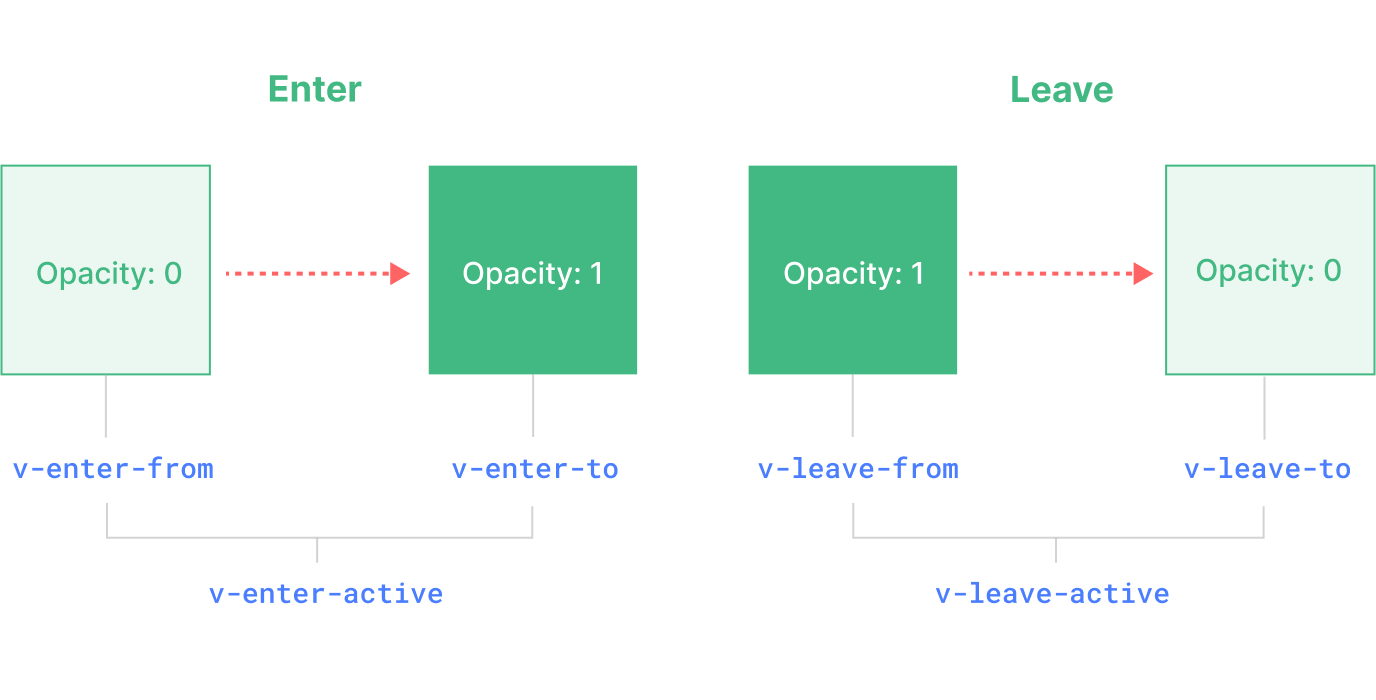
\includegraphics{./img/transition-classes.f0f7b3c9.png} 
\end{center}

\columnratio{0.55}
\begin{paracol}{2}
 
\switchcolumn[0]*%%%%%%%
\begin{enumerate}
\item
  \texttt{v-enter-from}: Starting state for enter. Added before the
  element is inserted, removed one frame after the element is inserted.
\item
  \texttt{v-enter-active}: Active state for enter. Applied during the
  entire entering phase. Added before the element is inserted, removed
  when the transition/animation finishes. This class can be used to
  define the duration, delay and easing curve for the entering
  transition.
\item
  \texttt{v-enter-to}: Ending state for enter. Added one frame after the
  element is inserted (at the same time \texttt{v-enter-from} is
  removed), removed when the transition/animation finishes.
\item
  \texttt{v-leave-from}: Starting state for leave. Added immediately
  when a leaving transition is triggered, removed after one frame.
\item
  \texttt{v-leave-active}: Active state for leave. Applied during the
  entire leaving phase. Added immediately when a leaving transition is
  triggered, removed when the transition/animation finishes. This class
  can be used to define the duration, delay and easing curve for the
  leaving transition.
\item
  \texttt{v-leave-to}: Ending state for leave. Added one frame after a
  leaving transition is triggered (at the same time
  \texttt{v-leave-from} is removed), removed when the
  transition/animation finishes.
\end{enumerate}
\switchcolumn
\begin{enumerate}
\item
  \texttt{v-enter-from}:进入动画的起始状态。在元素插入之前添加,在元素插入完成后的下一帧移除。
\item
  \texttt{v-enter-active}:进入动画的生效状态。应用于整个进入动画阶段。在元素被插入之前添加,在过渡或动画完成之后移除。这个
  class 可以被用来定义进入动画的持续时间、延迟与速度曲线类型。
\item
  \texttt{v-enter-to}:进入动画的结束状态。在元素插入完成后的下一帧被添加
  (也就是 \texttt{v-enter-from}
  被移除的同时),在过渡或动画完成之后移除。
\item
  \texttt{v-leave-from}:离开动画的起始状态。在离开过渡效果被触发时立即添加,在一帧后被移除。
\item
  \texttt{v-leave-active}:离开动画的生效状态。应用于整个离开动画阶段。在离开过渡效果被触发时立即添加,在过渡或动画完成之后移除。这个
  class 可以被用来定义离开动画的持续时间、延迟与速度曲线类型。
\item
  \texttt{v-leave-to}:离开动画的结束状态。在一个离开动画被触发后的下一帧被添加
  (也就是 \texttt{v-leave-from}
  被移除的同时),在过渡或动画完成之后移除。
\end{enumerate}
\switchcolumn[0]*%%%%%%%
\texttt{v-enter-active} and \texttt{v-leave-active} give us the ability
to specify different easing curves for enter / leave transitions, which
we'll see an example of in the following sections.
\switchcolumn
\texttt{v-enter-active} 和 \texttt{v-leave-active}
给我们提供了为进入和离开动画指定不同速度曲线的能力,我们将在下面的小节中看到一个示例。 
\end{paracol}

\columnratio{0.55}
\begin{paracol}{2}
 
\switchcolumn[0]*%%%%%%%
\subsubsection{Named Transitions}
\switchcolumn
\subsubsection{为过渡效果命名}
\switchcolumn[0]*%%%%%%%
A transition can be named via the \texttt{name} prop:
\switchcolumn
我们可以给 \texttt{\textless{}Transition\textgreater{}} 组件传一个
\texttt{name} prop 来声明一个过渡效果名:
\switchcolumn[0]*%%%%%%%
\begin{codeHtml}
<Transition name="fade">
  ...
</Transition>
\end{codeHtml}
\switchcolumn
\begin{codeHtml}
<Transition name="fade">
  ...
</Transition>
\end{codeHtml}
\switchcolumn[0]*%%%%%%%
For a named transition, its transition classes will be prefixed with its
name instead of \texttt{v}. For example, the applied class for the above
transition will be \texttt{fade-enter-active} instead of
\texttt{v-enter-active}. The CSS for the fade transition should look
like this:
\switchcolumn
对于一个有名字的过渡效果,对它起作用的过渡 class 会以其名字而不是
\texttt{v} 作为前缀。比如,上方例子中被应用的 class 将会是
\texttt{fade-enter-active} 而不是
\texttt{v-enter-active}。这个``fade''过渡的 class 应该是这样:
\switchcolumn[0]*%%%%%%%
\begin{codeCss}
.fade-enter-active,
.fade-leave-active {
  transition: opacity 0.5s ease;
}
.fade-enter-from,
.fade-leave-to {
  opacity: 0;
}
\end{codeCss}
\switchcolumn
\begin{codeCss}
.fade-enter-active,
.fade-leave-active {
  transition: opacity 0.5s ease;
}
.fade-enter-from,
.fade-leave-to {
  opacity: 0;
}
\end{codeCss}
\end{paracol}

\columnratio{0.55}
\begin{paracol}{2}
 
\switchcolumn[0]*%%%%%%%
\subsubsection{CSS Transitions}
\switchcolumn
\subsubsection{CSS 的 transition}
\switchcolumn[0]*%%%%%%%
\texttt{\textless{}Transition\textgreater{}} is most commonly used in
combination with
\href{https://developer.mozilla.org/en-US/docs/Web/CSS/CSS_Transitions/Using_CSS_transitions}{native
CSS transitions}, as seen in the basic example above. The
\texttt{transition} CSS property is a shorthand that allows us to
specify multiple aspects of a transition, including properties that
should be animated, duration of the transition, and
\href{https://developer.mozilla.org/en-US/docs/Web/CSS/easing-function}{easing
curves}.
\switchcolumn
\texttt{\textless{}Transition\textgreater{}}
一般都会搭配\href{https://developer.mozilla.org/en-US/docs/Web/CSS/CSS_Transitions/Using_CSS_transitions}{原生
CSS 过渡}一起使用,正如你在上面的例子中所看到的那样。这个
\texttt{transition} CSS
属性是一个简写形式,使我们可以一次定义一个过渡的各个方面,包括需要执行动画的属性、持续时间和\href{https://developer.mozilla.org/en-US/docs/Web/CSS/easing-function}{速度曲线}。
\switchcolumn[0]*%%%%%%%
Here is a more advanced example that transitions multiple properties,
with different durations and easing curves for enter and leave:
\switchcolumn
下面是一个更高级的例子,它使用了不同的持续时间和速度曲线来过渡多个属性:
\switchcolumn[0]*%%%%%%%
\begin{codeHtml}
<Transition name="slide-fade">
  <p v-if="show">hello</p>
</Transition>
\end{codeHtml}
\switchcolumn
\begin{codeHtml}
<Transition name="slide-fade">
  <p v-if="show">hello</p>
</Transition>
\end{codeHtml}
\switchcolumn[0]*%%%%%%%
\begin{codeCss}
/*
  进入和离开动画可以使用不同
  持续时间和速度曲线。
*/
.slide-fade-enter-active {
  transition: all 0.3s ease-out;
}
.slide-fade-leave-active {
  transition: all 0.8s cubic-bezier(1, 0.5, 0.8, 1);
}
.slide-fade-enter-from,
.slide-fade-leave-to {
  transform: translateX(20px);
  opacity: 0;
}
\end{codeCss}
\switchcolumn
\begin{codeCss}
/*
  进入和离开动画可以使用不同
  持续时间和速度曲线。
*/
.slide-fade-enter-active {
  transition: all 0.3s ease-out;
}
.slide-fade-leave-active {
  transition: all 0.8s cubic-bezier(1, 0.5, 0.8, 1);
}
.slide-fade-enter-from,
.slide-fade-leave-to {
  transform: translateX(20px);
  opacity: 0;
}
\end{codeCss}
\switchcolumn[0]*%%%%%%%
\href{https://play.vuejs.org/\#eNqFkc9uwjAMxl/F6wXQKIVNk1AX0HbZC4zDDr2E4EK0NIkStxtDvPviFQ0OSFzyx/m+n+34kL16P+lazMpMRBW0J4hIrV9WVjfeBYIDBKzhCHVwDQySdFDZyipnY5Lu3BcsWDCk0OKosqLoKcmfLoSNN5KQbyTWLZGz8KKMVp+LKju573ivsuXKbbcG4d3oDcI9vMkNiqL3JD+AWAVpoyadGFY2yATW5nVSJj9rkspDl+v6hE/hHRrjRMEdpdfiDEkBUVxWaEWkveHj5AzO0RKGXCrSHcKBIfSPKEEaA9PJYwSUEXPX0nNlj8y6RBiUHd5AzCOodq1VvsYfjWE4G6fgEy/zMcxG17B9ZTyX8bV85C5y1S40ZX/kdj+GD1P/zVQA56XStC9h2idJI/z7huz4CxoVvE4=}{Try
it in the Playground}
\switchcolumn
\href{https://play.vuejs.org/\#eNqFkc9uwjAMxl/F6wXQKIVNk1AX0HbZC4zDDr2E4EK0NIkStxtDvPviFQ0OSFzyx/m+n+34kL16P+lazMpMRBW0J4hIrV9WVjfeBYIDBKzhCHVwDQySdFDZyipnY5Lu3BcsWDCk0OKosqLoKcmfLoSNN5KQbyTWLZGz8KKMVp+LKju573ivsuXKbbcG4d3oDcI9vMkNiqL3JD+AWAVpoyadGFY2yATW5nVSJj9rkspDl+v6hE/hHRrjRMEdpdfiDEkBUVxWaEWkveHj5AzO0RKGXCrSHcKBIfSPKEEaA9PJYwSUEXPX0nNlj8y6RBiUHd5AzCOodq1VvsYfjWE4G6fgEy/zMcxG17B9ZTyX8bV85C5y1S40ZX/kdj+GD1P/zVQA56XStC9h2idJI/z7huz4CxoVvE4=}{在演练场中尝试一下}
\end{paracol}

\columnratio{0.55}
\begin{paracol}{2}
 
\switchcolumn[0]*%%%%%%%
\subsubsection{CSS Animations}
\switchcolumn
\subsubsection{CSS 的 animation}
\switchcolumn[0]*%%%%%%%
\href{https://developer.mozilla.org/en-US/docs/Web/CSS/CSS_Animations/Using_CSS_animations}{Native
CSS animations} are applied in the same way as CSS transitions, with the
difference being that \texttt{*-enter-from} is not removed immediately
after the element is inserted, but on an \texttt{animationend} event.
\switchcolumn
\href{https://developer.mozilla.org/en-US/docs/Web/CSS/CSS_Animations/Using_CSS_animations}{原生
CSS 动画}和 CSS transition
的应用方式基本上是相同的,只有一点不同,那就是 \texttt{*-enter-from}
不是在元素插入后立即移除,而是在一个 \texttt{animationend}
事件触发时被移除。
\switchcolumn[0]*%%%%%%%
For most CSS animations, we can simply declare them under the
\texttt{*-enter-active} and \texttt{*-leave-active} classes. Here's an
example:
\switchcolumn
对于大多数的 CSS 动画,我们可以简单地在 \texttt{*-enter-active} 和
\texttt{*-leave-active} class 下声明它们。下面是一个示例:
\switchcolumn[0]*%%%%%%%
\begin{codeHtml}
<Transition name="bounce">
  <p v-if="show" style="text-align: center;">
    Hello here is some bouncy text!
  </p>
</Transition>
\end{codeHtml}
\switchcolumn
\begin{codeHtml}
<Transition name="bounce">
  <p v-if="show" style="text-align: center;">
    Hello here is some bouncy text!
  </p>
</Transition>
\end{codeHtml}
\switchcolumn[0]*%%%%%%%
\begin{codeCss}
.bounce-enter-active {
  animation: bounce-in 0.5s;
}
.bounce-leave-active {
  animation: bounce-in 0.5s reverse;
}
@keyframes bounce-in {
  0% {
    transform: scale(0);
  }
  50% {
    transform: scale(1.25);
  }
  100% {
    transform: scale(1);
  }
}
\end{codeCss}
\switchcolumn
\begin{codeCss}
.bounce-enter-active {
  animation: bounce-in 0.5s;
}
.bounce-leave-active {
  animation: bounce-in 0.5s reverse;
}
@keyframes bounce-in {
  0% {
    transform: scale(0);
  }
  50% {
    transform: scale(1.25);
  }
  100% {
    transform: scale(1);
  }
}
\end{codeCss}
\switchcolumn[0]*%%%%%%%
\href{https://play.vuejs.org/\#eNqNksGOgjAQhl9lJNmoBwRNvCAa97YP4JFLbQZsLG3TDqzG+O47BaOezCYkpfB9/0wHbsm3c4u+w6RIyiC9cgQBqXO7yqjWWU9wA4813KH2toUpo9PKVEZaExg92V/YRmBGvsN5ZcpsTGGfN4St04Iw7qg8dkTWwF5qJc/bKnnYk7hWye5gm0ZjmY0YKwDlwQsTFCnWjGiRpaPtjETG43smHPSpqh9pVQKBrjpyrfCNMilZV8Aqd5cNEF4oFVo1pgCJhtBvnjEAP6i1hRN6BBUg2BZhKHUdvMmjWhYHE9dXY/ygzN4PasqhB75djM2mQ7FUSFI9wi0GCJ6uiHYxVsFUGcgX67CpzP0lahQ9/k/kj9CjDzgG7M94rT1PLLxhQ0D+Na4AFI9QW98WEKTQOMvnLAOwDrD+wC0Xq/Ubusw/sU+QL/45hskk9z8Bddbn}{Try
it in the Playground}
\switchcolumn
\href{https://play.vuejs.org/\#eNqNksGOgjAQhl9lJNmoBwRNvCAa97YP4JFLbQZsLG3TDqzG+O47BaOezCYkpfB9/0wHbsm3c4u+w6RIyiC9cgQBqXO7yqjWWU9wA4813KH2toUpo9PKVEZaExg92V/YRmBGvsN5ZcpsTGGfN4St04Iw7qg8dkTWwF5qJc/bKnnYk7hWye5gm0ZjmY0YKwDlwQsTFCnWjGiRpaPtjETG43smHPSpqh9pVQKBrjpyrfCNMilZV8Aqd5cNEF4oFVo1pgCJhtBvnjEAP6i1hRN6BBUg2BZhKHUdvMmjWhYHE9dXY/ygzN4PasqhB75djM2mQ7FUSFI9wi0GCJ6uiHYxVsFUGcgX67CpzP0lahQ9/k/kj9CjDzgG7M94rT1PLLxhQ0D+Na4AFI9QW98WEKTQOMvnLAOwDrD+wC0Xq/Ubusw/sU+QL/45hskk9z8Bddbn}{在演练场中尝试一下}
\end{paracol}

\columnratio{0.55}
\begin{paracol}{2}
 
\switchcolumn[0]*%%%%%%%
\subsubsection{Custom Transition Classes}
\switchcolumn
\subsubsection{自定义过渡 class}
\switchcolumn[0]*%%%%%%%
You can also specify custom transition classes by passing the following
props to \texttt{\textless{}Transition\textgreater{}}:
\switchcolumn
你也可以向 \texttt{\textless{}Transition\textgreater{}} 传递以下的 props
来指定自定义的过渡 class:
\switchcolumn[0]*%%%%%%%
\begin{itemize}
\item
  \texttt{enter-from-class}
\item
  \texttt{enter-active-class}
\item
  \texttt{enter-to-class}
\item
  \texttt{leave-from-class}
\item
  \texttt{leave-active-class}
\item
  \texttt{leave-to-class}
\end{itemize}
\switchcolumn
\begin{itemize}
\item
  \texttt{enter-from-class}
\item
  \texttt{enter-active-class}
\item
  \texttt{enter-to-class}
\item
  \texttt{leave-from-class}
\item
  \texttt{leave-active-class}
\item
  \texttt{leave-to-class}
\end{itemize}
\switchcolumn[0]*%%%%%%%
These will override the conventional class names. This is especially
useful when you want to combine Vue's transition system with an existing
CSS animation library, such as
\href{https://daneden.github.io/animate.css/}{Animate.css}:
\switchcolumn
你传入的这些 class 会覆盖相应阶段的默认 class 名。这个功能在你想要在 Vue
的动画机制下集成其他的第三方 CSS 动画库时非常有用,比如
\href{https://daneden.github.io/animate.css/}{Animate.css}:
\switchcolumn[0]*%%%%%%%
\begin{codeHtml}
<!-- 假设你已经在页面中引入了 Animate.css -->
<Transition
  name="custom-classes"
  enter-active-class="animate__animated animate__tada"
  leave-active-class="animate__animated animate__bounceOutRight"
>
  <p v-if="show">hello</p>
</Transition>
\end{codeHtml}
\switchcolumn
\begin{codeHtml}
<!-- 假设你已经在页面中引入了 Animate.css -->
<Transition
  name="custom-classes"
  enter-active-class="animate__animated animate__tada"
  leave-active-class="animate__animated animate__bounceOutRight"
>
  <p v-if="show">hello</p>
</Transition>
\end{codeHtml}
\switchcolumn[0]*%%%%%%%
\href{https://play.vuejs.org/\#eNqNUctuwjAQ/BXXF9oDsZB6ogbRL6hUcbSEjLMhpn7JXtNWiH/vhqS0R3zxPmbWM+szf02pOVXgSy6LyTYhK4A1rVWwPsWM7MwydOzCuhw9mxF0poIKJoZC0D5+stUAeMRc4UkFKcYpxKcEwSenEYYM5b4ixsA2xlnzsVJ8Yj8Mt+LrbTwcHEgxwojCmNxmHYpFG2kaoxO0B2KaWjD6uXG6FCiKj00ICHmuDdoTjD2CavJBCna7KWjZrYK61b9cB5pI93P3sQYDbxXf7aHHccpVMolO7DS33WSQjPXgXJRi2Cl1xZ8nKkjxf0dBFvx2Q7iZtq94j5jKUgjThmNpjIu17ZzO0JjohT7qL+HsvohJWWNKEc/NolncKt6Goar4y/V7rg/wyw9zrLOy}{Try
it in the Playground}
\switchcolumn
\href{https://play.vuejs.org/\#eNqNUctuwjAQ/BXXF9oDsZB6ogbRL6hUcbSEjLMhpn7JXtNWiH/vhqS0R3zxPmbWM+szf02pOVXgSy6LyTYhK4A1rVWwPsWM7MwydOzCuhw9mxF0poIKJoZC0D5+stUAeMRc4UkFKcYpxKcEwSenEYYM5b4ixsA2xlnzsVJ8Yj8Mt+LrbTwcHEgxwojCmNxmHYpFG2kaoxO0B2KaWjD6uXG6FCiKj00ICHmuDdoTjD2CavJBCna7KWjZrYK61b9cB5pI93P3sQYDbxXf7aHHccpVMolO7DS33WSQjPXgXJRi2Cl1xZ8nKkjxf0dBFvx2Q7iZtq94j5jKUgjThmNpjIu17ZzO0JjohT7qL+HsvohJWWNKEc/NolncKt6Goar4y/V7rg/wyw9zrLOy}{在演练场中尝试一下}
\end{paracol}

\columnratio{0.55}
\begin{paracol}{2}
 
\switchcolumn[0]*%%%%%%%
\subsubsection{Using Transitions and Animations Together}
\switchcolumn
\subsubsection{同时使用 transition 和 animation}
\switchcolumn[0]*%%%%%%%
Vue needs to attach event listeners in order to know when a transition
has ended. It can either be \texttt{transitionend} or
\texttt{animationend}, depending on the type of CSS rules applied. If
you are only using one or the other, Vue can automatically detect the
correct type.
\switchcolumn
Vue 需要附加事件监听器,以便知道过渡何时结束。可以是
\texttt{transitionend} 或 \texttt{animationend},这取决于你所应用的 CSS
规则。如果你仅仅使用二者的其中之一,Vue 可以自动探测到正确的类型。
\switchcolumn[0]*%%%%%%%
However, in some cases you may want to have both on the same element,
for example having a CSS animation triggered by Vue, along with a CSS
transition effect on hover. In these cases, you will have to explicitly
declare the type you want Vue to care about by passing the \texttt{type}
prop, with a value of either \texttt{animation} or \texttt{transition}:
\switchcolumn
然而在某些场景中,你或许想要在同一个元素上同时使用它们两个。举例来说,Vue
触发了一个 CSS 动画,同时鼠标悬停触发另一个 CSS
过渡。此时你需要显式地传入 \texttt{type} prop 来声明,告诉 Vue
需要关心哪种类型,传入的值是 \texttt{animation} 或 \texttt{transition}:
\switchcolumn[0]*%%%%%%%
\begin{codeHtml}
<Transition type="animation">...</Transition>
\end{codeHtml}
\switchcolumn
\begin{codeHtml}
<Transition type="animation">...</Transition>
\end{codeHtml}
\end{paracol}

\columnratio{0.55}
\begin{paracol}{2}
 
\switchcolumn[0]*%%%%%%%
\subsubsection{Nested Transitions and Explicit Transition Durations}
\switchcolumn
\subsubsection{深层级过渡与显式过渡时长}
\switchcolumn[0]*%%%%%%%
Although the transition classes are only applied to the direct child
element in \texttt{\textless{}Transition\textgreater{}}, we can
transition nested elements using nested CSS selectors:
\switchcolumn
尽管过渡 class 仅能应用在 \texttt{\textless{}Transition\textgreater{}}
的直接子元素上,我们还是可以使用深层级的 CSS
选择器,在深层级的元素上触发过渡效果。
\switchcolumn[0]*%%%%%%%
\begin{codeHtml}
<Transition name="nested">
  <div v-if="show" class="outer">
    <div class="inner">
      Hello
    </div>
  </div>
</Transition>
\end{codeHtml}
\switchcolumn
\begin{codeHtml}
<Transition name="nested">
  <div v-if="show" class="outer">
    <div class="inner">
      Hello
    </div>
  </div>
</Transition>
\end{codeHtml}
\switchcolumn[0]*%%%%%%%
\begin{codeCss}
/* 应用于嵌套元素的规则 */
.nested-enter-active .inner,
.nested-leave-active .inner {
  transition: all 0.3s ease-in-out;
}
.nested-enter-from .inner,
.nested-leave-to .inner {
  transform: translateX(30px);
  opacity: 0;
}
/* ... 省略了其他必要的 CSS */
\end{codeCss}
\switchcolumn
\begin{codeCss}
/* 应用于嵌套元素的规则 */
.nested-enter-active .inner,
.nested-leave-active .inner {
  transition: all 0.3s ease-in-out;
}
.nested-enter-from .inner,
.nested-leave-to .inner {
  transform: translateX(30px);
  opacity: 0;
}
/* ... 省略了其他必要的 CSS */
\end{codeCss}
\switchcolumn[0]*%%%%%%%
We can even add a transition delay to the nested element on enter, which
creates a staggered enter animation sequence:
\switchcolumn
我们甚至可以在深层元素上添加一个过渡延迟,从而创建一个带渐进延迟的动画序列:
\switchcolumn[0]*%%%%%%%
\begin{codeCss}
/* 延迟嵌套元素的进入以获得交错效果 */
.nested-enter-active .inner {
  transition-delay: 0.25s;
}
\end{codeCss}
\switchcolumn
\begin{codeCss}
/* 延迟嵌套元素的进入以获得交错效果 */
.nested-enter-active .inner {
  transition-delay: 0.25s;
}
\end{codeCss}
\switchcolumn[0]*%%%%%%%
However, this creates a small issue. By default, the
\texttt{\textless{}Transition\textgreater{}} component attempts to
automatically figure out when the transition has finished by listening
to the \textbf{first} \texttt{transitionend} or \texttt{animationend}
event on the root transition element. With a nested transition, the
desired behavior should be waiting until the transitions of all inner
elements have finished.
\switchcolumn
然而,这会带来一个小问题。默认情况下,\texttt{\textless{}Transition\textgreater{}}
组件会通过监听过渡根元素上的\textbf{第一个} \texttt{transitionend} 或者
\texttt{animationend}
事件来尝试自动判断过渡何时结束。而在嵌套的过渡中,期望的行为应该是等待所有内部元素的过渡完成。
\switchcolumn[0]*%%%%%%%
In such cases you can specify an explicit transition duration (in
milliseconds) using the \texttt{duration} prop on the
\texttt{\textless{}transition\textgreater{}} component. The total
duration should match the delay plus transition duration of the inner
element:
\switchcolumn
在这种情况下,你可以通过向 \texttt{\textless{}Transition\textgreater{}}
组件传入 \texttt{duration} prop 来显式指定过渡的持续时间
(以毫秒为单位)。总持续时间应该匹配延迟加上内部元素的过渡持续时间:
\switchcolumn[0]*%%%%%%%
\begin{codeHtml}
<Transition :duration="550">...</Transition>
\end{codeHtml}
\switchcolumn
\begin{codeHtml}
<Transition :duration="550">...</Transition>
\end{codeHtml}
\switchcolumn[0]*%%%%%%%
\href{https://play.vuejs.org/\#eNqVVd9v0zAQ/leO8LAfrE3HNKSFbgKmSYMHQNAHkPLiOtfEm2NHttN2mvq/c7bTNi1jgFop9t13d9995ziPyfumGc5bTLJkbLkRjQOLrm2uciXqRhsHj2BwBiuYGV3DAUEPcpUrrpUlaKUXcOkBh860eJSrcRqzUDxtHNaNZA5pBzCets5pBe+4FPz+Mk+66Bf+mSdXE12WEsdphMWQiWHKCicoLCtaw/yKIs/PR3kCitVIG4XWYUEJfATFFGIO84GYdRUIyCWzlra6dWg2wA66dgqlts7c+d8tSqk34JTQ6xqb9TjdUiTDOO21TFvrHqRfDkPpExiGKvBITjdl/L40ulVFBi8R8a3P17CiEKrM4GzULIOlFmpQoSgrl8HpKFpX3kFZu2y0BNhJxznvwaJCA1TEYcC4E3MkKp1VIptjZ43E3KajDJiUMBqeWUBmcUBUqJGYOT2GAiV7gJAA9Iy4GyoBKLH2z+N0W3q/CMC2yCCkyajM63Mbc+9z9mfvZD+b071MM23qLC69+j8PvX5HQUDdMC6cL7BOTtQXCJwpas/qHhWIBdYtWGgtDWNttWTmThu701pf1W6+v1Hd8Xbz+k+VQxmv8i7Fv1HZn+g/iv2nRkjzbd6npf/Rkz49DifQ3dLZBBYOJzC4rqgCwsUbmLYlCAUVU4XsCd1NrCeRHcYXb1IJC/RX2hEYCwJTvHYVMZoavbBI09FmU+LiFSzIh0AIXy1mqZiFKaKCmVhiEVJ7GftHZTganUZ56EYLL3FykjhL195MlMM7qxXdmEGDPOG6boRE86UJVPMki+p4H01WLz4Fm78hSdBo5xXy+yfsd3bpbXny1SA1M8c82fgcMyW66L75/hmXtN44a120ktDPOL+h1bL1HCPsA42DaPdwge3HcO/TOCb2ZumQJtA15Yl65Crg84S+BdfPtL6lezY8C3GkZ7L6Bc1zNR0=}{Try
it in the Playground}
\switchcolumn
\href{https://play.vuejs.org/\#eNqVVMtu2zAQ/JWtekjiRo80cIGoStCil3yADy2gC02tJCIUKZCUncDwv3cpyrbstmgLGxC53J2ZnaW0i772fbIZMMqjwnIjegcW3dA/lUp0vTYOdmCwhj3URndwRalXpSoV18pSaqu38OgTrp0Z8KZURRpQqJ42DrteMoe0AyjWg3NawRcuBX95LKOp+p1/ltHTSjeNxCINaaFkZZiywgkqqwbD/IIKl8usjECxDmmj0DqsqN4XUEklNrCJRT0RUCKXzFra6sGhOSZOqYdDodTpsHT+94xS6mNyStkHjuO6SE8KKVCks45pa92b9MtkpL6FZGSBHR26NeMvjdGDqnJ4j4ifPV7PqkqoJof7rH8dI51QcYuiaV0Od1mI7v0BoU5otAQ4g+Ocz9KCQzEq0hAz7sQGScoUlcg2OEWDMHfsKAcmJWTJvQVkFmOSQo0E5HQBFUr2BiMA6Jq0G6IAlNj55yI9UV+SAJxI4hEmJ5qPSxuwLzX7q3d7ieb0DKnWpsvD0rv/49r7dzMaqHvGhfMEB3CSvkXgTFF7Vs+kQCA4tGBhsDSMQ9RSmDtt7Flrc1en+f4i9ex0mtd/ujzSeJfPJf5NyuVE/9HsPzVCnp9wf2/995n16WK8ge6Z7iaw8XICg28tMSA8fIL10IBQ0DJVyZnR08RmFtkkvHirVligv9KOkrGiZKrXriVFa6O3Fmk62hwpHj7Als4QKMOzBZSWWVgjKqjFK1YjtLdxflWSLLsL9tAHbXyJo/1PJETL1g==}{在演练场中尝试一下}
\switchcolumn[0]*%%%%%%%
If necessary, you can also specify separate values for enter and leave
durations using an object:
\switchcolumn
如果有必要的话,你也可以用对象的形式传入,分开指定进入和离开所需的时间:
\switchcolumn[0]*%%%%%%%
\begin{codeHtml}
<Transition :duration="{ enter: 500, leave: 800 }">...</Transition>
\end{codeHtml}
\switchcolumn
\begin{codeHtml}
<Transition :duration="{ enter: 500, leave: 800 }">...</Transition>
\end{codeHtml}
\end{paracol}

\columnratio{0.55}
\begin{paracol}{2}
 
\switchcolumn[0]*%%%%%%%
\subsubsection{Performance Considerations}
\switchcolumn
\subsubsection{性能考量}
\switchcolumn[0]*%%%%%%%
You may notice that the animations shown above are mostly using
properties like \texttt{transform} and \texttt{opacity}. These
properties are efficient to animate because:
\switchcolumn
你可能注意到我们上面例子中展示的动画所用到的 CSS 属性大多是
\texttt{transform} 和 \texttt{opacity}
之类的。用这些属性制作动画非常高效,因为:
\switchcolumn[0]*%%%%%%%
\begin{enumerate}
\item
  They do not affect the document layout during the animation, so they
  do not trigger expensive CSS layout calculation on every animation
  frame.
\item
  Most modern browsers can leverage GPU hardware acceleration when
  animating \texttt{transform}.
\end{enumerate}
\switchcolumn
\begin{enumerate}
\item
  他们在动画过程中不会影响到 DOM 结构,因此不会每一帧都触发昂贵的 CSS
  布局重新计算。
\item
  大多数的现代浏览器都可以在执行 \texttt{transform} 动画时利用 GPU
  进行硬件加速。
\end{enumerate}
\switchcolumn[0]*%%%%%%%
In comparison, properties like \texttt{height} or \texttt{margin} will
trigger CSS layout, so they are much more expensive to animate, and
should be used with caution. We can check resources like
\href{https://csstriggers.com/}{CSS-Triggers} to see which properties
will trigger layout if we animate them.
\switchcolumn
相比之下,像 \texttt{height} 或者 \texttt{margin} 这样的属性会触发 CSS
布局变动,因此执行它们的动画效果更昂贵,需要谨慎使用。我们可以在
\href{https://csstriggers.com/}{CSS-Triggers}
这类的网站查询哪些属性会在执行动画时触发 CSS 布局变动。
\end{paracol}

\columnratio{0.55}
\begin{paracol}{2}
 
\switchcolumn[0]*%%%%%%%
\subsection{JavaScript Hooks}
\switchcolumn
\subsection{JavaScript 钩子}
\switchcolumn[0]*%%%%%%%
You can hook into the transition process with JavaScript by listening to
events on the \texttt{\textless{}Transition\textgreater{}} component:
\switchcolumn
你可以通过监听 \texttt{\textless{}Transition\textgreater{}}
组件事件的方式在过渡过程中挂上钩子函数:
\switchcolumn[0]*%%%%%%%
\begin{codeHtml}
<Transition
  @before-enter="onBeforeEnter"
  @enter="onEnter"
  @after-enter="onAfterEnter"
  @enter-cancelled="onEnterCancelled"
  @before-leave="onBeforeLeave"
  @leave="onLeave"
  @after-leave="onAfterLeave"
  @leave-cancelled="onLeaveCancelled"
>
  <!-- ... -->
</Transition>
\end{codeHtml}
\switchcolumn
\begin{codeHtml}
<Transition
  @before-enter="onBeforeEnter"
  @enter="onEnter"
  @after-enter="onAfterEnter"
  @enter-cancelled="onEnterCancelled"
  @before-leave="onBeforeLeave"
  @leave="onLeave"
  @after-leave="onAfterLeave"
  @leave-cancelled="onLeaveCancelled"
>
  <!-- ... -->
</Transition>
\end{codeHtml}
\switchcolumn[0]*%%%%%%%
\begin{codeJs}
// 在元素被插入到 DOM 之前被调用
// 用这个来设置元素的 "enter-from" 状态
function onBeforeEnter(el) {}
// 在元素被插入到 DOM 之后的下一帧被调用
// 用这个来开始进入动画
function onEnter(el, done) {
  // 调用回调函数 done 表示过渡结束
  // 如果与 CSS 结合使用,则这个回调是可选参数
  done()
}
// 当进入过渡完成时调用。
function onAfterEnter(el) {}
// 当进入过渡在完成之前被取消时调用
function onEnterCancelled(el) {}
// 在 leave 钩子之前调用
// 大多数时候,你应该只会用到 leave 钩子
function onBeforeLeave(el) {}
// 在离开过渡开始时调用
// 用这个来开始离开动画
function onLeave(el, done) {
  // 调用回调函数 done 表示过渡结束
  // 如果与 CSS 结合使用,则这个回调是可选参数
  done()
}
// 在离开过渡完成、
// 且元素已从 DOM 中移除时调用
function onAfterLeave(el) {}
// 仅在 v-show 过渡中可用
function onLeaveCancelled(el) {}
\end{codeJs}
\switchcolumn
\begin{codeJs}
// 在元素被插入到 DOM 之前被调用
// 用这个来设置元素的 "enter-from" 状态
function onBeforeEnter(el) {}
// 在元素被插入到 DOM 之后的下一帧被调用
// 用这个来开始进入动画
function onEnter(el, done) {
  // 调用回调函数 done 表示过渡结束
  // 如果与 CSS 结合使用,则这个回调是可选参数
  done()
}
// 当进入过渡完成时调用。
function onAfterEnter(el) {}
// 当进入过渡在完成之前被取消时调用
function onEnterCancelled(el) {}
// 在 leave 钩子之前调用
// 大多数时候,你应该只会用到 leave 钩子
function onBeforeLeave(el) {}
// 在离开过渡开始时调用
// 用这个来开始离开动画
function onLeave(el, done) {
  // 调用回调函数 done 表示过渡结束
  // 如果与 CSS 结合使用,则这个回调是可选参数
  done()
}
// 在离开过渡完成、
// 且元素已从 DOM 中移除时调用
function onAfterLeave(el) {}
// 仅在 v-show 过渡中可用
function onLeaveCancelled(el) {}
\end{codeJs}
\switchcolumn[0]*%%%%%%%
These hooks can be used in combination with CSS transitions / animations
or on their own.
\switchcolumn
这些钩子可以与 CSS 过渡或动画结合使用,也可以单独使用。
\switchcolumn[0]*%%%%%%%
When using JavaScript-only transitions, it is usually a good idea to add
the \texttt{:css="false"} prop. This explicitly tells Vue to skip auto
CSS transition detection. Aside from being slightly more performant,
this also prevents CSS rules from accidentally interfering with the
transition:
\switchcolumn
在使用仅由 JavaScript 执行的动画时,最好是添加一个 \texttt{:css="false"}
prop。这显式地向 Vue 表明可以跳过对 CSS
过渡的自动探测。除了性能稍好一些之外,还可以防止 CSS
规则意外地干扰过渡效果。
\switchcolumn[0]*%%%%%%%
\begin{codeCss}
<Transition
  ...
  :css="false"
>
  ...
</Transition>
\end{codeCss}
\switchcolumn
\begin{codeCss}
<Transition
  ...
  :css="false"
>
  ...
</Transition>
\end{codeCss}
\switchcolumn[0]*%%%%%%%
With \texttt{:css="false"}, we are also fully responsible for
controlling when the transition ends. In this case, the \texttt{done}
callbacks are required for the \texttt{@enter} and \texttt{@leave}
hooks. Otherwise, the hooks will be called synchronously and the
transition will finish immediately.
\switchcolumn
在有了 \texttt{:css="false"}
后,我们就自己全权负责控制什么时候过渡结束了。这种情况下对于
\texttt{@enter} 和 \texttt{@leave} 钩子来说,回调函数 \texttt{done}
就是必须的。否则,钩子将被同步调用,过渡将立即完成。
\switchcolumn[0]*%%%%%%%
Here's a demo using the \href{https://greensock.com/}{GreenSock library}
to perform the animations. You can, of course, use any other animation
library you want, for example \href{https://animejs.com/}{Anime.js} or
\href{https://motion.dev/}{Motion One}.
\switchcolumn
这里是使用 \href{https://greensock.com/}{GreenSock
库}执行动画的一个示例,你也可以使用任何你想要的库,比如
\href{https://animejs.com/}{Anime.js} 或者
\href{https://motion.dev/}{Motion One}。
\switchcolumn[0]*%%%%%%%
\href{https://play.vuejs.org/\#eNqNVMtu2zAQ/JUti8I2YD3i1GigKmnaorcCveTQArpQFCWzlkiCpBwHhv+9Sz1qKYckJ3FnlzvD2YVO5KvW4aHlJCGpZUZoB5a7Vt9lUjRaGQcnMLyEM5RGNbDA0sX/VGWpHnB/xEQmmZIWe+zUI9z6m0tnWr7ymbKVzAklQclvvFSG/5COmyWvV3DKJHTdQiRHZN0jAJbRmv9OIA432/UE+jODlKZMuKcErnx8RrazP8woR7I1FEryKaVTU8aiNdRfwWZTQtQwi1HAGF/YB4BTyxNY8JpaJ1go5K/WLTfhdg1Xq8V4SX5Xja65w0ovaCJ8Jvsnpwc+l525F2XH4ac3Cj8mcB3HbxE9qnvFMRzJ0K3APuhIjPefmTTyvWBAGvWbiDuIgeNYRh3HCCDNW+fQmHtWC7a/zciwaO/8NyN3D6qqap5GfVnXAC89GCqt8Bp77vu827+A+53AJrOFzMhQdMnO8dqPpMO74Yx4wqxFtKS1HbBOMdIX4gAMffVp71+Qq2NG4BCIcngBKk8jLOvfGF30IpBGEwcwtO6p9sdwbNXPIadsXxnVyiKB9x83+c3N9WePN9RUQgZO6QQ2sT524KMo3M5Pf4h3XFQ7NwFyZQpuAkML0doEtvEHhPvRDPRkTfq/QNDgRvy1SuIvpFOSDQmbkWTckf7hHsjIzjltkyhqpd5XIVNN5HNfGlW09eAcMp3J+R+pEn7L}{Try
it in the Playground}
\switchcolumn
\href{https://play.vuejs.org/\#eNqNVMtu2zAQ/JUti8I2YD3i1GigKmnaorcCveTQArpQFCWzlkiCpBwHhv+9Sz1qKYckJ3FnlzvD2YVO5KvW4aHlJCGpZUZoB5a7Vt9lUjRaGQcnMLyEM5RGNbDA0sX/VGWpHnB/xEQmmZIWe+zUI9z6m0tnWr7ymbKVzAklQclvvFSG/5COmyWvV3DKJHTdQiRHZN0jAJbRmv9OIA432/UE+jODlKZMuKcErnx8RrazP8woR7I1FEryKaVTU8aiNdRfwWZTQtQwi1HAGF/YB4BTyxNY8JpaJ1go5K/WLTfhdg1Xq8V4SX5Xja65w0ovaCJ8Jvsnpwc+l525F2XH4ac3Cj8mcB3HbxE9qnvFMRzJ0K3APuhIjPefmTTyvWBAGvWbiDuIgeNYRh3HCCDNW+fQmHtWC7a/zciwaO/8NyN3D6qqap5GfVnXAC89GCqt8Bp77vu827+A+53AJrOFzMhQdMnO8dqPpMO74Yx4wqxFtKS1HbBOMdIX4gAMffVp71+Qq2NG4BCIcngBKk8jLOvfGF30IpBGEwcwtO6p9sdwbNXPIadsXxnVyiKB9x83+c3N9WePN9RUQgZO6QQ2sT524KMo3M5Pf4h3XFQ7NwFyZQpuAkML0doEtvEHhPvRDPRkTfq/QNDgRvy1SuIvpFOSDQmbkWTckf7hHsjIzjltkyhqpd5XIVNN5HNfGlW09eAcMp3J+R+pEn7L}{在演练场中尝试一下}
\end{paracol}

\columnratio{0.55}
\begin{paracol}{2}
 
\switchcolumn[0]*%%%%%%%
\subsection{Reusable Transitions}
\switchcolumn
\subsection{可复用过渡效果}
\switchcolumn[0]*%%%%%%%
Transitions can be reused through Vue's component system. To create a
reusable transition, we can create a component that wraps the
\texttt{\textless{}Transition\textgreater{}} component and passes down
the slot content:
\switchcolumn
得益于 Vue
的组件系统,过渡效果是可以被封装复用的。要创建一个可被复用的过渡,我们需要为
\texttt{\textless{}Transition\textgreater{}}
组件创建一个包装组件,并向内传入插槽内容:
\switchcolumn[0]*%%%%%%%
\begin{codeHtml}
<!-- MyTransition.vue -->
<script>
// JavaScript 钩子逻辑...
</script>
<template>
  <!-- 包装内置的 Transition 组件 -->
  <Transition
    name="my-transition"
    @enter="onEnter"
    @leave="onLeave">
    <slot></slot> <!-- 向内传递插槽内容 -->
  </Transition>
</template>
<style>
/*
  必要的 CSS...
  注意:避免在这里使用 <style scoped>
  因为那不会应用到插槽内容上
*/
</style>
\end{codeHtml}
\switchcolumn
\begin{codeHtml}
<!-- MyTransition.vue -->
<script>
// JavaScript 钩子逻辑...
</script>
<template>
  <!-- 包装内置的 Transition 组件 -->
  <Transition
    name="my-transition"
    @enter="onEnter"
    @leave="onLeave">
    <slot></slot> <!-- 向内传递插槽内容 -->
  </Transition>
</template>
<style>
/*
  必要的 CSS...
  注意:避免在这里使用 <style scoped>
  因为那不会应用到插槽内容上
*/
</style>
\end{codeHtml}
\switchcolumn[0]*%%%%%%%
Now \texttt{MyTransition} can be imported and used just like the
built-in version:
\switchcolumn
现在 \texttt{MyTransition} 可以在导入后像内置组件那样使用了:
\switchcolumn[0]*%%%%%%%
\begin{codeHtml}
<MyTransition>
  <div v-if="show">Hello</div>
</MyTransition>
\end{codeHtml}
\switchcolumn
\begin{codeHtml}
<MyTransition>
  <div v-if="show">Hello</div>
</MyTransition>
\end{codeHtml}
\end{paracol}

\columnratio{0.55}
\begin{paracol}{2}
 
\switchcolumn[0]*%%%%%%%
\subsection{Transition on Appear}
\switchcolumn
\subsection{出现时过渡}
\switchcolumn[0]*%%%%%%%
If you also want to apply a transition on the initial render of a node,
you can add the \texttt{appear} prop:
\switchcolumn
如果你想在某个节点初次渲染时应用一个过渡效果,你可以添加 \texttt{appear}
prop:
\switchcolumn[0]*%%%%%%%
\begin{codeHtml}
<Transition appear>
  ...
</Transition>
\end{codeHtml}
\switchcolumn
\begin{codeHtml}
<Transition appear>
  ...
</Transition>
\end{codeHtml}
\switchcolumn[0]*%%%%%%%
\subsection{Transition Between Elements}
\switchcolumn
\subsection{元素间过渡}
\switchcolumn[0]*%%%%%%%
In addition to toggling an element with \texttt{v-if} / \texttt{v-show},
we can also transition between two elements using \texttt{v-if} /
\texttt{v-else} / \texttt{v-else-if}, as long as we make sure that there
is only one element being shown at any given moment:
\switchcolumn
除了通过 \texttt{v-if} / \texttt{v-show} 切换一个元素,我们也可以通过
\texttt{v-if} / \texttt{v-else} / \texttt{v-else-if}
在几个组件间进行切换,只要确保任一时刻只会有一个元素被渲染即可:
\switchcolumn[0]*%%%%%%%
\begin{codeHtml}
<Transition>
  <button v-if="docState === 'saved'">Edit</button>
  <button v-else-if="docState === 'edited'">Save</button>
  <button v-else-if="docState === 'editing'">Cancel</button>
</Transition>
\end{codeHtml}
\switchcolumn
\begin{codeHtml}
<Transition>
  <button v-if="docState === 'saved'">Edit</button>
  <button v-else-if="docState === 'edited'">Save</button>
  <button v-else-if="docState === 'editing'">Cancel</button>
</Transition>
\end{codeHtml}
\switchcolumn[0]*%%%%%%%
\href{https://play.vuejs.org/\#eNqdk8tu2zAQRX9loI0SoLLcFN2ostEi6BekmwLa0NTYJkKRBDkSYhj+9wxJO3ZegBGu+Lhz7syQ3Bd/nJtNIxZN0QbplSMISKNbdkYNznqCPXhcwwHW3g5QsrTsTGekNYGgt/KBBCEsouimDGLCvrztTFtnGGN4QTg4zbK4ojY4YSDQTuOiKwbhN8pUXm221MDd3D11xfJeK/kIZEHupEagrbfjZssxzAgNs5nALIC2VxNILUJg1IpMxWmRUAY9U6IZ2/3zwgRFyhowYoieQaseq9ElDaTRrkYiVkyVWrPiXNdiAcequuIkPo3fMub5Sg4l9oqSevmXZ22dwR8YoQ74kdsL4Go7ZTbR74HT/KJfJlxleGrG8l4YifqNYVuf251vqOYr4llbXz4C06b75+ns1a3BPsb0KrBy14Aymnerlbby8Vc8cTajG35uzFITpu0t5ufzHQdeH6LBsezEO0eJVbB6pBiVVLPTU6jQEPpKyMj8dnmgkQs+HmQcvVTIQK1hPrv7GQAFt9eO9Bk6fZ8Ub52Qiri8eUo+4dbWD02exh79v/nBP+H2PStnwz/jelJ1geKvk/peHJ4BoRZYow==}{Try
it in the Playground}
\switchcolumn
\href{https://play.vuejs.org/\#eNqdk8tu2zAQRX9loI0SoLLcFN2ostEi6BekmwLa0NTYJkKRBDkSYhj+9wxJO3ZegBGu+Lhz7syQ3Bd/nJtNIxZN0QbplSMISKNbdkYNznqCPXhcwwHW3g5QsrTsTGekNYGgt/KBBCEsouimDGLCvrztTFtnGGN4QTg4zbK4ojY4YSDQTuOiKwbhN8pUXm221MDd3D11xfJeK/kIZEHupEagrbfjZssxzAgNs5nALIC2VxNILUJg1IpMxWmRUAY9U6IZ2/3zwgRFyhowYoieQaseq9ElDaTRrkYiVkyVWrPiXNdiAcequuIkPo3fMub5Sg4l9oqSevmXZ22dwR8YoQ74kdsL4Go7ZTbR74HT/KJfJlxleGrG8l4YifqNYVuf251vqOYr4llbXz4C06b75+ns1a3BPsb0KrBy14Aymnerlbby8Vc8cTajG35uzFITpu0t5ufzHQdeH6LBsezEO0eJVbB6pBiVVLPTU6jQEPpKyMj8dnmgkQs+HmQcvVTIQK1hPrv7GQAFt9eO9Bk6fZ8Ub52Qiri8eUo+4dbWD02exh79v/nBP+H2PStnwz/jelJ1geKvk/peHJ4BoRZYow==}{在演练场中尝试一下}
\end{paracol}

\columnratio{0.55}
\begin{paracol}{2}
 
\switchcolumn[0]*%%%%%%%
\subsection{Transition Modes}
\switchcolumn
\subsection{过渡模式}
\switchcolumn[0]*%%%%%%%
In the previous example, the entering and leaving elements are animated
at the same time, and we had to make them \texttt{position:\ absolute}
to avoid the layout issue when both elements are present in the DOM.
\switchcolumn
在之前的例子中,进入和离开的元素都是在同时开始动画的,因此我们不得不将它们设为
\texttt{position:\ absolute} 以避免二者同时存在时出现的布局问题。
\switchcolumn[0]*%%%%%%%
However, in some cases this isn't an option, or simply isn't the desired
behavior. We may want the leaving element to be animated out first, and
for the entering element to only be inserted \textbf{after} the leaving
animation has finished. Orchestrating such animations manually would be
very complicated - luckily, we can enable this behavior by passing
\texttt{\textless{}Transition\textgreater{}} a \texttt{mode} prop:
\switchcolumn
然而,很多情况下这可能并不符合需求。我们可能想要先执行离开动画,然后在其完成\textbf{之后}再执行元素的进入动画。手动编排这样的动画是非常复杂的,好在我们可以通过向
\texttt{\textless{}Transition\textgreater{}} 传入一个 \texttt{mode} prop
来实现这个行为:
\switchcolumn[0]*%%%%%%%
\begin{codeHtml}
<Transition mode="out-in">
  ...
</Transition>
\end{codeHtml}
\switchcolumn
\begin{codeHtml}
<Transition mode="out-in">
  ...
</Transition>
\end{codeHtml}
\switchcolumn[0]*%%%%%%%
Here's the previous demo with \texttt{mode="out-in"}:
\switchcolumn
将之前的例子改为 \texttt{mode="out-in"} 后是这样:
\switchcolumn[0]*%%%%%%%
\texttt{\textless{}Transition\textgreater{}} also supports
\texttt{mode="in-out"}, although it's much less frequently used.
\switchcolumn
\texttt{\textless{}Transition\textgreater{}} 也支持
\texttt{mode="in-out"},虽然这并不常用。
\switchcolumn[0]*%%%%%%%
\subsection{Transition Between Components}
\switchcolumn
\subsection{组件间过渡}
\switchcolumn[0]*%%%%%%%
\texttt{\textless{}Transition\textgreater{}} can also be used around
\href{https://vuejs.org/guide/essentials/component-basics.html\#dynamic-components}{dynamic
components}:
\switchcolumn
\texttt{\textless{}Transition\textgreater{}}
也可以作用于\href{https://cn.vuejs.org/guide/essentials/component-basics.html\#dynamic-components}{动态组件}之间的切换:
\switchcolumn[0]*%%%%%%%
\begin{codeHtml}
<Transition name="fade" mode="out-in">
  <component :is="activeComponent"></component>
</Transition>
\end{codeHtml}
\switchcolumn
\begin{codeHtml}
<Transition name="fade" mode="out-in">
  <component :is="activeComponent"></component>
</Transition>
\end{codeHtml}
\switchcolumn[0]*%%%%%%%
\href{https://play.vuejs.org/\#eNqtksFugzAMhl/F4tJNKtDLLoxWKnuDacdcUnC3SCGJiMmEqr77EkgLbXfYYZyI8/v77dinZG9M5npMiqS0dScMgUXqzY4p0RrdEZzAfnEp9fc7HuEMx063sPIZq6viTbdmHy+yfDwF5K2guhFUUcBUnkNvcelBGrjTooHaC7VCRXBAoT6hQTRyAH2w2DlsmKq1sgS8JuEwUCfxdgF7Gqt5ZqrMp+58X/5A2BrJCcOJSskPKP0v+K8UyvQENBjcsqTjjdAsAZe2ukHpI3dm/q5wXPZBPFqxZAf7gCrzGfufDlVwqB4cPjqurCChFSjeBvGRN+iTA9afdE+pUD43FjG/bSHsb667Mr9qJot89vCBMl8+oiotDTL8ZsE39UnYpRN0fQlK5A5jEE6BSVdiAdrwWtAAm+zFAnKLr0ydA3pJDDt0x/PrMrJifgGbKdFPfCwpWU+TuWz5omzfVCNcfJJ5geL8pqtFn5E07u7fSHFOj6TzDyUDNEM=}{Try
it in the Playground}
\switchcolumn
\href{https://play.vuejs.org/\#eNqtksFugzAMhl/F4tJNKtDLLoxWKnuDacdcUnC3SCGJiMmEqr77EkgLbXfYYZyI8/v77dinZG9M5npMiqS0dScMgUXqzY4p0RrdEZzAfnEp9fc7HuEMx063sPIZq6viTbdmHy+yfDwF5K2guhFUUcBUnkNvcelBGrjTooHaC7VCRXBAoT6hQTRyAH2w2DlsmKq1sgS8JuEwUCfxdgF7Gqt5ZqrMp+58X/5A2BrJCcOJSskPKP0v+K8UyvQENBjcsqTjjdAsAZe2ukHpI3dm/q5wXPZBPFqxZAf7gCrzGfufDlVwqB4cPjqurCChFSjeBvGRN+iTA9afdE+pUD43FjG/bSHsb667Mr9qJot89vCBMl8+oiotDTL8ZsE39UnYpRN0fQlK5A5jEE6BSVdiAdrwWtAAm+zFAnKLr0ydA3pJDDt0x/PrMrJifgGbKdFPfCwpWU+TuWz5omzfVCNcfJJ5geL8pqtFn5E07u7fSHFOj6TzDyUDNEM=}{在演练场中尝试一下}
\end{paracol}

\columnratio{0.55}
\begin{paracol}{2}
 
\switchcolumn[0]*%%%%%%%
\subsection{Dynamic Transitions}
\switchcolumn
\subsection{动态过渡}
\switchcolumn[0]*%%%%%%%
\texttt{\textless{}Transition\textgreater{}} props like \texttt{name}
can also be dynamic! It allows us to dynamically apply different
transitions based on state change:
\switchcolumn
\texttt{\textless{}Transition\textgreater{}} 的 props (比如
\texttt{name})
也可以是动态的!这让我们可以根据状态变化动态地应用不同类型的过渡:
\switchcolumn[0]*%%%%%%%
\begin{codeHtml}
<Transition :name="transitionName">
  <!-- ... -->
</Transition>
\end{codeHtml}
\switchcolumn
\begin{codeHtml}
<Transition :name="transitionName">
  <!-- ... -->
</Transition>
\end{codeHtml}
\switchcolumn[0]*%%%%%%%
This can be useful when you've defined CSS transitions / animations
using Vue's transition class conventions and want to switch between
them.
\switchcolumn
这个特性的用处是可以提前定义好多组 CSS 过渡或动画的
class,然后在它们之间动态切换。
\switchcolumn[0]*%%%%%%%
You can also apply different behavior in JavaScript transition hooks
based on the current state of your component. Finally, the ultimate way
of creating dynamic transitions is through
\href{https://vuejs.org/guide/built-ins/transition.html\#reusable-transitions}{reusable
transition components} that accept props to change the nature of the
transition(s) to be used. It may sound cheesy, but the only limit really
is your imagination.
\switchcolumn
你也可以根据你的组件的当前状态在 JavaScript
过渡钩子中应用不同的行为。最后,创建动态过渡的终极方式还是创建\href{https://cn.vuejs.org/guide/built-ins/transition.html\#reusable-transitions}{可复用的过渡组件},并让这些组件根据动态的
props
来改变过渡的效果。掌握了这些技巧后,就真的只有你想不到,没有做不到的了。
\switchcolumn[0]*%%%%%%%
\begin{center}\rule{0.5\linewidth}{0.5pt}\end{center}
\switchcolumn
\begin{center}\rule{0.5\linewidth}{0.5pt}\end{center}
\switchcolumn[0]*%%%%%%%
\textbf{Related}
\switchcolumn
\textbf{参考}
\switchcolumn[0]*%%%%%%%
\begin{itemize}
\item
  \href{https://vuejs.org/api/built-in-components.html\#transition}{``
  API reference}
\end{itemize}
\switchcolumn
\begin{itemize}
\item
  \href{https://cn.vuejs.org/api/built-in-components.html\#transition}{``
  API 参考}
\end{itemize}
\end{paracol}


\columnratio{0.55}
\begin{paracol}{2}
 
\switchcolumn[0]*%%%%%%%
\section{TransitionGroup}
\switchcolumn
\section{TransitionGroup}
\switchcolumn[0]*%%%%%%%
\texttt{\textless{}TransitionGroup\textgreater{}} is a built-in
component designed for animating the insertion, removal, and order
change of elements or components that are rendered in a list.
\switchcolumn
\texttt{\textless{}TransitionGroup\textgreater{}} 是一个内置组件,用于对
\texttt{v-for} 列表中的元素或组件的插入、移除和顺序改变添加动画效果。
\switchcolumn[0]*%%%%%%%
\subsection{Differences from \textless Transition\textgreater{}}
\switchcolumn
\subsection{和 \textless Transition\textgreater{} 的区别}
\switchcolumn[0]*%%%%%%%
\texttt{\textless{}TransitionGroup\textgreater{}} supports the same
props, CSS transition classes, and JavaScript hook listeners as
\texttt{\textless{}Transition\textgreater{}}, with the following
differences:
\switchcolumn
\texttt{\textless{}TransitionGroup\textgreater{}} 支持和
\texttt{\textless{}Transition\textgreater{}} 基本相同的 props、CSS 过渡
class 和 JavaScript 钩子监听器,但有以下几点区别:
\switchcolumn[0]*%%%%%%%
\begin{itemize}
\item
  By default, it doesn't render a wrapper element. But you can specify
  an element to be rendered with the \texttt{tag} prop.
\item
  \href{https://vuejs.org/guide/built-ins/transition.html\#transition-modes}{Transition
  modes} are not available, because we are no longer alternating between
  mutually exclusive elements.
\item
  Elements inside are \textbf{always required} to have a unique
  \texttt{key} attribute.
\item
  CSS transition classes will be applied to individual elements in the
  list, \textbf{not} to the group / container itself.
\end{itemize}
\switchcolumn
\begin{itemize}
\item
  默认情况下,它不会渲染一个容器元素。但你可以通过传入 \texttt{tag} prop
  来指定一个元素作为容器元素来渲染。
\item
  \href{https://cn.vuejs.org/guide/built-ins/transition.html\#transition-modes}{过渡模式}在这里不可用,因为我们不再是在互斥的元素之间进行切换。
\item
  列表中的每个元素都\textbf{必须}有一个独一无二的 \texttt{key}
  attribute。
\item
  CSS 过渡 class 会被应用在列表内的元素上,\textbf{而不是}容器元素上。
\end{itemize}
\switchcolumn[0]*%%%%%%%
\begin{vueQuote}{TIP}
When used in
\href{https://vuejs.org/guide/essentials/component-basics.html\#in-dom-template-parsing-caveats}{in-DOM
templates}, it should be referenced as
\texttt{\textless{}transition-group\textgreater{}}.
\end{vueQuote} 
\switchcolumn
\begin{vueQuote}{TIP}
当在
\href{https://cn.vuejs.org/guide/essentials/component-basics.html\#in-dom-template-parsing-caveats}{DOM
内模板}中使用时,组件名需要写为
\texttt{\textless{}transition-group\textgreater{}}。
\end{vueQuote} 
\end{paracol}

\columnratio{0.55}
\begin{paracol}{2}
 
\switchcolumn[0]*%%%%%%%
\subsection{Enter / Leave Transitions}
\switchcolumn
\subsection{进入 / 离开动画}
\switchcolumn[0]*%%%%%%%
Here is an example of applying enter / leave transitions to a
\texttt{v-for} list using
\texttt{\textless{}TransitionGroup\textgreater{}}:
\switchcolumn
这里是 \texttt{\textless{}TransitionGroup\textgreater{}} 对一个
\texttt{v-for} 列表添加进入 / 离开动画的示例:
\switchcolumn[0]*%%%%%%%
\begin{codeHtml}
<TransitionGroup name="list" tag="ul">
  <li v-for="item in items" :key="item">
    {{ item }}
  </li>
</TransitionGroup>
\end{codeHtml}
\switchcolumn
\begin{codeHtml}
<TransitionGroup name="list" tag="ul">
  <li v-for="item in items" :key="item">
    {{ item }}
  </li>
</TransitionGroup>
\end{codeHtml}
\switchcolumn[0]*%%%%%%%
\begin{codeCss}
.list-enter-active,
.list-leave-active {
  transition: all 0.5s ease;
}
.list-enter-from,
.list-leave-to {
  opacity: 0;
  transform: translateX(30px);
}
\end{codeCss}
\switchcolumn
\begin{codeCss}
.list-enter-active,
.list-leave-active {
  transition: all 0.5s ease;
}
.list-enter-from,
.list-leave-to {
  opacity: 0;
  transform: translateX(30px);
}
\end{codeCss}
\end{paracol}

\columnratio{0.55}
\begin{paracol}{2}
 
\switchcolumn[0]*%%%%%%%
\subsection{Move Transitions}
\switchcolumn
\subsection{移动动画}
\switchcolumn[0]*%%%%%%%
The above demo has some obvious flaws: when an item is inserted or
removed, its surrounding items instantly "jump" into place instead of
moving smoothly. We can fix this by adding a few additional CSS rules:
\switchcolumn
上面的示例有一些明显的缺陷:当某一项被插入或移除时,它周围的元素会立即发生``跳跃''而不是平稳地移动。我们可以通过添加一些额外的
CSS 规则来解决这个问题:
\switchcolumn[0]*%%%%%%%
\begin{codeCss}
.list-move, /* 对移动中的元素应用的过渡 */
.list-enter-active,
.list-leave-active {
  transition: all 0.5s ease;
}
.list-enter-from,
.list-leave-to {
  opacity: 0;
  transform: translateX(30px);
}
/* 确保将离开的元素从布局流中删除
  以便能够正确地计算移动的动画。 */
.list-leave-active {
  position: absolute;
}
\end{codeCss}
\switchcolumn
\begin{codeCss}
.list-move, /* 对移动中的元素应用的过渡 */
.list-enter-active,
.list-leave-active {
  transition: all 0.5s ease;
}
.list-enter-from,
.list-leave-to {
  opacity: 0;
  transform: translateX(30px);
}
/* 确保将离开的元素从布局流中删除
  以便能够正确地计算移动的动画。 */
.list-leave-active {
  position: absolute;
}
\end{codeCss}
\switchcolumn[0]*%%%%%%%
Now it looks much better - even animating smoothly when the whole list
is shuffled:
\switchcolumn
现在它看起来好多了,甚至对整个列表执行洗牌的动画也都非常流畅:
\switchcolumn[0]*%%%%%%%
\href{https://vuejs.org/examples/\#list-transition}{Full Example}
\switchcolumn
\href{https://cn.vuejs.org/examples/\#list-transition}{完整的示例}
\end{paracol}

\columnratio{0.55}
\begin{paracol}{2}
 
\switchcolumn[0]*%%%%%%%
\subsection{Staggering List Transitions}
\switchcolumn
\subsection{渐进延迟列表动画}
\switchcolumn[0]*%%%%%%%
By communicating with JavaScript transitions through data attributes,
it's also possible to stagger transitions in a list. First, we render
the index of an item as a data attribute on the DOM element:
\switchcolumn
通过在 JavaScript 钩子中读取元素的 data
attribute,我们可以实现带渐进延迟的列表动画。首先,我们把每一个元素的索引渲染为该元素上的一个
data attribute:
\switchcolumn[0]*%%%%%%%
\begin{codeHtml}
<TransitionGroup
  tag="ul"
  :css="false"
  @before-enter="onBeforeEnter"
  @enter="onEnter"
  @leave="onLeave"
>
  <li
    v-for="(item, index) in computedList"
    :key="item.msg"
    :data-index="index"
  >
    {{ item.msg }}
  </li>
</TransitionGroup>
\end{codeHtml}
\switchcolumn
\begin{codeHtml}
<TransitionGroup
  tag="ul"
  :css="false"
  @before-enter="onBeforeEnter"
  @enter="onEnter"
  @leave="onLeave"
>
  <li
    v-for="(item, index) in computedList"
    :key="item.msg"
    :data-index="index"
  >
    {{ item.msg }}
  </li>
</TransitionGroup>
\end{codeHtml}
\switchcolumn[0]*%%%%%%%
Then, in JavaScript hooks, we animate the element with a delay based on
the data attribute. This example is using the
\href{https://greensock.com/}{GreenSock library} to perform the
animation:
\switchcolumn
接着,在 JavaScript 钩子中,我们基于当前元素的 data attribute
对该元素的进场动画添加一个延迟。以下是一个基于
\href{https://greensock.com/}{GreenSock library} 的动画示例:
\switchcolumn[0]*%%%%%%%
\begin{codeJs}
function onEnter(el, done) {
  gsap.to(el, {
    opacity: 1,
    height: '1.6em',
    delay: el.dataset.index * 0.15,
    onComplete: done
  })
}
\end{codeJs}
\switchcolumn
\begin{codeJs}
function onEnter(el, done) {
  gsap.to(el, {
    opacity: 1,
    height: '1.6em',
    delay: el.dataset.index * 0.15,
    onComplete: done
  })
}
\end{codeJs}
\switchcolumn[0]*%%%%%%%
\href{https://play.vuejs.org/\#eNqlVMuu0zAQ/ZVRNklRm7QLWETtBW4FSFCxYkdYmGSSmjp28KNQVfl3xk7SFyvEponPGc+cOTPNOXrbdenRYZRHa1Nq3lkwaF33VEjedkpbOIPGeg6lajtnsYIeaq1aiOlSfAlqDOtG3L8SUchSSWNBcPrZwNdCAqVqTZND/KxdibBDjKGf3xIfWXngCNs9k4/Udu/KA3xWWnPz1zW0sOOP6CcnG3jv9ImIQn67SvrpUJ9IE/WVxPHsSkw97gbN0zFJZrB5grNPrskcLUNXac2FRZ0k3GIbIvxLSsVTq3bqF+otM5jMUi5L4So0SSicHplwOKOyfShdO1lariQo+Yy10vhO+qwoZkNFFKmxJ4Gp6ljJrRe+vMP3yJu910swNXqXcco1h0pJHDP6CZHEAAcAYMydwypYCDAkJRdX6Sts4xGtUDAKotIVs9Scpd4q/A0vYJmuXo5BSm7JOIEW81DVo77VR207ZEf8F23LB23T+X9VrbNh82nn6UAz7ASzSCeANZe0AnBctIqqbIoojLCIIBvoL5pJw31DH7Ry3VDKsoYinSii4ZyXxhBQM2Fwwt58D7NeoB8QkXfDvwRd2XtceOsCHkwc8KCINAk+vADJppQUFjZ0DsGVGT3uFn1KSjoPeKLoaYtvCO/rIlz3vH9O5FiU/nXny/pDT6YGKZngg0/Zg1GErrMbp6N5NHxJFi3N/4dRkj5IYf5ULxCmiPJpI4rIr4kHimhvbWfyLHOyOzQpNZZ57jXNy4nRGFLTR/0fWBqe7w==}{Full
Example in the Playground}
\switchcolumn
\href{https://play.vuejs.org/\#eNqlVMuu0zAQ/ZVRNklRm7QLWETtBW4FSFCxYkdYmGSSmjp28KNQVfl3xk7SFyvEponPGc+cOTPNOXrbdenRYZRHa1Nq3lkwaF33VEjedkpbOIPGeg6lajtnsYIeaq1aiOlSfAlqDOtG3L8SUchSSWNBcPrZwNdCAqVqTZND/KxdibBDjKGf3xIfWXngCNs9k4/Udu/KA3xWWnPz1zW0sOOP6CcnG3jv9ImIQn67SvrpUJ9IE/WVxPHsSkw97gbN0zFJZrB5grNPrskcLUNXac2FRZ0k3GIbIvxLSsVTq3bqF+otM5jMUi5L4So0SSicHplwOKOyfShdO1lariQo+Yy10vhO+qwoZkNFFKmxJ4Gp6ljJrRe+vMP3yJu910swNXqXcco1h0pJHDP6CZHEAAcAYMydwypYCDAkJRdX6Sts4xGtUDAKotIVs9Scpd4q/A0vYJmuXo5BSm7JOIEW81DVo77VR207ZEf8F23LB23T+X9VrbNh82nn6UAz7ASzSCeANZe0AnBctIqqbIoojLCIIBvoL5pJw31DH7Ry3VDKsoYinSii4ZyXxhBQM2Fwwt58D7NeoB8QkXfDvwRd2XtceOsCHkwc8KCINAk+vADJppQUFjZ0DsGVGT3uFn1KSjoPeKLoaYtvCO/rIlz3vH9O5FiU/nXny/pDT6YGKZngg0/Zg1GErrMbp6N5NHxJFi3N/4dRkj5IYf5ULxCmiPJpI4rIr4kHimhvbWfyLHOyOzQpNZZ57jXNy4nRGFLTR/0fWBqe7w==}{在演练场中查看完整示例}
\switchcolumn[0]*%%%%%%%
\begin{center}\rule{0.5\linewidth}{0.5pt}\end{center}
\switchcolumn
\begin{center}\rule{0.5\linewidth}{0.5pt}\end{center}
\switchcolumn[0]*%%%%%%%
\textbf{Related}
\switchcolumn
\textbf{参考}
\switchcolumn[0]*%%%%%%%
\begin{itemize}
\item
  \href{https://vuejs.org/api/built-in-components.html\#transitiongroup}{``
  API reference}
\end{itemize}
\switchcolumn
\begin{itemize}
\item
  \href{https://cn.vuejs.org/api/built-in-components.html\#transitiongroup}{``
  API 参考}
\end{itemize}
\end{paracol}


\columnratio{0.55}
\begin{paracol}{2}
 
\switchcolumn[0]*%%%%%%%
\section{KeepAlive}
\switchcolumn
\section{KeepAlive}
\switchcolumn[0]*%%%%%%%
\texttt{\textless{}KeepAlive\textgreater{}} is a built-in component that
allows us to conditionally cache component instances when dynamically
switching between multiple components.
\switchcolumn
\texttt{\textless{}KeepAlive\textgreater{}}
是一个内置组件,它的功能是在多个组件间动态切换时缓存被移除的组件实例。
\switchcolumn[0]*%%%%%%%
\subsection{Basic Usage}
\switchcolumn
\subsection{基本使用}
\switchcolumn[0]*%%%%%%%
In the Component Basics chapter, we introduced the syntax for
\href{https://vuejs.org/guide/essentials/component-basics.html\#dynamic-components}{Dynamic
Components}, using the \texttt{\textless{}component\textgreater{}}
special element:
\switchcolumn
在组件基础章节中,我们已经介绍了通过特殊的
\texttt{\textless{}component\textgreater{}}
元素来实现\href{https://cn.vuejs.org/guide/essentials/component-basics.html\#dynamic-components}{动态组件}的用法: 
\switchcolumn[0]*%%%%%%%
\begin{codeHtml}
<component :is="activeComponent" />
\end{codeHtml}
\switchcolumn
\begin{codeHtml}
<component :is="activeComponent" />
\end{codeHtml}
\switchcolumn[0]*%%%%%%%
By default, an active component instance will be unmounted when
switching away from it. This will cause any changed state it holds to be
lost. When this component is displayed again, a new instance will be
created with only the initial state.
\switchcolumn
默认情况下,一个组件实例在被替换掉后会被销毁。这会导致它丢失其中所有已变化的状态------当这个组件再一次被显示时,会创建一个只带有初始状态的新实例。
\switchcolumn[0]*%%%%%%%
In the example below, we have two stateful components - A contains a
counter, while B contains a message synced with an input via
\texttt{v-model}. Try updating the state of one of them, switch away,
and then switch back to it:
\switchcolumn
在下面的例子中,你会看到两个有状态的组件------A 有一个计数器,而 B
有一个通过 \texttt{v-model} 同步 input
框输入内容的文字展示。尝试先更改一下任意一个组件的状态,然后切走,再切回来:
\switchcolumn[0]*%%%%%%%
You'll notice that when switched back, the previous changed state would
have been reset.
\switchcolumn
你会发现在切回来之后,之前已更改的状态都被重置了。 
\switchcolumn[0]*%%%%%%%
Creating fresh component instance on switch is normally useful behavior,
but in this case, we'd really like the two component instances to be
preserved even when they are inactive. To solve this problem, we can
wrap our dynamic component with the
\texttt{\textless{}KeepAlive\textgreater{}} built-in component:
\switchcolumn
在切换时创建新的组件实例通常是有意义的,但在这个例子中,我们的确想要组件能在被``切走''的时候保留它们的状态。要解决这个问题,我们可以用
\texttt{\textless{}KeepAlive\textgreater{}}
内置组件将这些动态组件包装起来:
\switchcolumn[0]*%%%%%%%
\begin{codeHtml}
<!-- 非活跃的组件将会被缓存! -->
<KeepAlive>
  <component :is="activeComponent" />
</KeepAlive>
\end{codeHtml}
\switchcolumn
\begin{codeHtml}
<!-- 非活跃的组件将会被缓存! -->
<KeepAlive>
  <component :is="activeComponent" />
</KeepAlive>
\end{codeHtml}
\switchcolumn[0]*%%%%%%%
Now, the state will be persisted across component switches:
\switchcolumn
现在,在组件切换时状态也能被保留了:
\switchcolumn[0]*%%%%%%%
\href{https://play.vuejs.org/\#eNqtUsFOwzAM/RWrl4IGC+cqq2h3RFw495K12YhIk6hJi1DVf8dJSllBaAJxi+2XZz8/j0lhzHboeZIl1NadMA4sd73JKyVaozsHI9hnJqV+feJHmODY6RZS/JEuiL1uTTEXtiREnnINKFeAcgZUqtbKOqj7ruPKwe6s2VVguq4UJXEynAkDx1sjmeMYAdBGDFBLZu2uShre6ioJeaxIduAyp0KZ3oF7MxwRHWsEQmC4bXXDJWbmxpjLBiZ7DwptMUFyKCiJNP/BWUbO8gvnA+emkGKIgkKqRrRWfh+Z8MIWwpySpfbxn6wJKMGV4IuSs0UlN1HVJae7bxYvBuk+2IOIq7sLnph8P9u5DJv5VfpWWLaGqTzwZTCOM/M0IaMvBMihd04ruK+lqF/8Ajxms8EFbCiJxR8khsP6ncQosLWnWV6a/kUf2nqu75Fby04chA0iPftaYryhz6NBRLjdtajpHZTWPio=}{Try
it in the Playground}
\switchcolumn
\href{https://play.vuejs.org/\#eNqtUsFOwzAM/RWrl4IGC+cqq2h3RFw495K12YhIk6hJi1DVf8dJSllBaAJxi+2XZz8/j0lhzHboeZIl1NadMA4sd73JKyVaozsHI9hnJqV+feJHmODY6RZS/JEuiL1uTTEXtiREnnINKFeAcgZUqtbKOqj7ruPKwe6s2VVguq4UJXEynAkDx1sjmeMYAdBGDFBLZu2uShre6ioJeaxIduAyp0KZ3oF7MxwRHWsEQmC4bXXDJWbmxpjLBiZ7DwptMUFyKCiJNP/BWUbO8gvnA+emkGKIgkKqRrRWfh+Z8MIWwpySpfbxn6wJKMGV4IuSs0UlN1HVJae7bxYvBuk+2IOIq7sLnph8P9u5DJv5VfpWWLaGqTzwZTCOM/M0IaMvBMihd04ruK+lqF/8Ajxms8EFbCiJxR8khsP6ncQosLWnWV6a/kUf2nqu75Fby04chA0iPftaYryhz6NBRLjdtajpHZTWPio=}{在演练场中尝试一下}
\switchcolumn[0]*%%%%%%%
\begin{vueQuote}{TIP}
When used in
\href{https://vuejs.org/guide/essentials/component-basics.html\#in-dom-template-parsing-caveats}{in-DOM
templates}, it should be referenced as
\texttt{\textless{}keep-alive\textgreater{}}.
\end{vueQuote} 
\switchcolumn
\begin{vueQuote}{TIP}
在
\href{https://cn.vuejs.org/guide/essentials/component-basics.html\#in-dom-template-parsing-caveats}{DOM
内模板}中使用时,它应该被写为
\texttt{\textless{}keep-alive\textgreater{}}。
\end{vueQuote} 
\switchcolumn[0]*%%%%%%%
\subsection{Include / Exclude}
\switchcolumn
\subsection{包含/排除}
\switchcolumn[0]*%%%%%%%
By default, \texttt{\textless{}KeepAlive\textgreater{}} will cache any
component instance inside. We can customize this behavior via the
\texttt{include} and \texttt{exclude} props. Both props can be a
comma-delimited string, a \texttt{RegExp}, or an array containing either
types:
\switchcolumn
\texttt{\textless{}KeepAlive\textgreater{}}
默认会缓存内部的所有组件实例,但我们可以通过 \texttt{include} 和
\texttt{exclude} prop 来定制该行为。这两个 prop
的值都可以是一个以英文逗号分隔的字符串、一个正则表达式,或是包含这两种类型的一个数组:
\switchcolumn[0]*%%%%%%%
\begin{codeHtml}
<!-- 以英文逗号分隔的字符串 -->
<KeepAlive include="a,b">
    <component :is="view" />
</KeepAlive>
<!-- 正则表达式 (需使用 `v-bind`) -->
<KeepAlive :include="/a|b/">
    <component :is="view" />
</KeepAlive>
<!-- 数组 (需使用 `v-bind`) -->
<KeepAlive :include="['a', 'b']">
    <component :is="view" />
</KeepAlive>
\end{codeHtml}
\switchcolumn
\begin{codeHtml}
<!-- 以英文逗号分隔的字符串 -->
<KeepAlive include="a,b">
  <component :is="view" />
</KeepAlive>
<!-- 正则表达式 (需使用 `v-bind`) -->
<KeepAlive :include="/a|b/">
  <component :is="view" />
</KeepAlive>
<!-- 数组 (需使用 `v-bind`) -->
<KeepAlive :include="['a', 'b']">
  <component :is="view" />
</KeepAlive>
\end{codeHtml}
\switchcolumn[0]*%%%%%%%
The match is checked against the component's
\href{https://vuejs.org/api/options-misc.html\#name}{\texttt{name}}
option, so components that need to be conditionally cached by
\texttt{KeepAlive} must explicitly declare a \texttt{name} option.
\switchcolumn
它会根据组件的
\href{https://cn.vuejs.org/api/options-misc.html\#name}{\texttt{name}}
选项进行匹配,所以组件如果想要条件性地被 \texttt{KeepAlive}
缓存,就必须显式声明一个 \texttt{name} 选项。
\switchcolumn[0]*%%%%%%%
\begin{vueQuote}{TIP}
Since version 3.2.34, a single-file component using
\texttt{\textless{}script\ setup\textgreater{}} will automatically infer
its \texttt{name} option based on the filename, removing the need to
manually declare the name.
\end{vueQuote} 
\switchcolumn
\begin{vueQuote}{TIP}
在 3.2.34 或以上的版本中,使用
\texttt{\textless{}script\ setup\textgreater{}}
的单文件组件会自动根据文件名生成对应的 \texttt{name}
选项,无需再手动声明。
\end{vueQuote} 
\switchcolumn[0]*%%%%%%%
\subsection{Max Cached Instances}
\switchcolumn
\subsection{最大缓存实例数}
\switchcolumn[0]*%%%%%%%
We can limit the maximum number of component instances that can be
cached via the \texttt{max} prop. When \texttt{max} is specified,
\texttt{\textless{}KeepAlive\textgreater{}} behaves like an
\href{https://en.wikipedia.org/wiki/Cache_replacement_policies\#Least_recently_used_(LRU)}{LRU
cache}: if the number of cached instances is about to exceed the
specified max count, the least recently accessed cached instance will be
destroyed to make room for the new one.
\switchcolumn
我们可以通过传入 \texttt{max} prop
来限制可被缓存的最大组件实例数。\texttt{\textless{}KeepAlive\textgreater{}}
的行为在指定了 \texttt{max} 后类似一个
\href{https://en.wikipedia.org/wiki/Cache_replacement_policies\#Least_recently_used_(LRU)}{LRU
缓存}:如果缓存的实例数量即将超过指定的那个最大数量,则最久没有被访问的缓存实例将被销毁,以便为新的实例腾出空间。
\switchcolumn[0]*%%%%%%%
\begin{codeHtml}
<KeepAlive :max="10">
  <component :is="activeComponent" />
</KeepAlive>
\end{codeHtml}
\switchcolumn
\begin{codeHtml}
<KeepAlive :max="10">
  <component :is="activeComponent" />
</KeepAlive>
\end{codeHtml}
\switchcolumn[0]*%%%%%%%
\subsection{Lifecycle of Cached Instance}
\switchcolumn
\subsection{缓存实例的生命周期}
\switchcolumn[0]*%%%%%%%
When a component instance is removed from the DOM but is part of a
component tree cached by \texttt{\textless{}KeepAlive\textgreater{}}, it
goes into a \textbf{deactivated} state instead of being unmounted. When
a component instance is inserted into the DOM as part of a cached tree,
it is \textbf{activated}.
\switchcolumn
当一个组件实例从 DOM 上移除但因为被
\texttt{\textless{}KeepAlive\textgreater{}}
缓存而仍作为组件树的一部分时,它将变为\textbf{不活跃}状态而不是被卸载。当一个组件实例作为缓存树的一部分插入到
DOM 中时,它将重新\textbf{被激活}。
\switchcolumn[0]*%%%%%%%
A kept-alive component can register lifecycle hooks for these two states
using
\href{https://vuejs.org/api/composition-api-lifecycle.html\#onactivated}{\texttt{onActivated()}}
and
\href{https://vuejs.org/api/composition-api-lifecycle.html\#ondeactivated}{\texttt{onDeactivated()}}:
\switchcolumn
一个持续存在的组件可以通过
\href{https://cn.vuejs.org/api/composition-api-lifecycle.html\#onactivated}{\texttt{onActivated()}}
和
\href{https://cn.vuejs.org/api/composition-api-lifecycle.html\#ondeactivated}{\texttt{onDeactivated()}}
注册相应的两个状态的生命周期钩子:
\switchcolumn[0]*%%%%%%%
\begin{codeHtml}
<script setup>
import { onActivated, onDeactivated } from 'vue'
onActivated(() => {
  // 调用时机为首次挂载
  // 以及每次从缓存中被重新插入时
})
onDeactivated(() => {
  // 在从 DOM 上移除、进入缓存
  // 以及组件卸载时调用
})
</script>
\end{codeHtml}
\switchcolumn
\begin{codeHtml}
<script setup>
import { onActivated, onDeactivated } from 'vue'
onActivated(() => {
  // 调用时机为首次挂载
  // 以及每次从缓存中被重新插入时
})
onDeactivated(() => {
  // 在从 DOM 上移除、进入缓存
  // 以及组件卸载时调用
})
</script>
\end{codeHtml}
\switchcolumn[0]*%%%%%%%
Note that:
\switchcolumn
请注意:
\switchcolumn[0]*%%%%%%%
\begin{itemize}
\item
  \texttt{onActivated} is also called on mount, and
  \texttt{onDeactivated} on unmount.
\item
  Both hooks work for not only the root component cached by
  \texttt{\textless{}KeepAlive\textgreater{}}, but also descendant
  components in the cached tree.
\end{itemize}
\switchcolumn
\begin{itemize}
\item
  \texttt{onActivated} 在组件挂载时也会调用,并且 \texttt{onDeactivated}
  在组件卸载时也会调用。
\item
  这两个钩子不仅适用于 \texttt{\textless{}KeepAlive\textgreater{}}
  缓存的根组件,也适用于缓存树中的后代组件。
\end{itemize}
\switchcolumn[0]*%%%%%%%
\begin{center}\rule{0.5\linewidth}{0.5pt}\end{center}
\switchcolumn
\begin{center}\rule{0.5\linewidth}{0.5pt}\end{center}
\switchcolumn[0]*%%%%%%%
\textbf{Related}
\switchcolumn
\textbf{参考}
\switchcolumn[0]*%%%%%%%
\begin{itemize}
\item
  \href{https://vuejs.org/api/built-in-components.html\#keepalive}{``
  API reference}
\end{itemize}
\switchcolumn
\begin{itemize}
\item
  \href{https://cn.vuejs.org/api/built-in-components.html\#keepalive}{``
  API 参考}
\end{itemize}
\end{paracol}
%todo 看
\columnratio{0.55}
\begin{paracol}{2}
\switchcolumn[0]*%%%%%%%
\section{Teleport}
\switchcolumn
\section{Teleport}
\switchcolumn[0]*%%%%%%%
\texttt{\textless{}Teleport\textgreater{}} is a built-in component that
allows us to "teleport" a part of a component's template into a DOM node
that exists outside the DOM hierarchy of that component.
\switchcolumn
\texttt{\textless{}Teleport\textgreater{}}
是一个内置组件,它可以将一个组件内部的一部分模板``传送''到该组件的 DOM
结构外层的位置去。
\switchcolumn[0]*%%%%%%%
\subsection{Basic Usage}
\switchcolumn
\subsection{基本用法}
\switchcolumn[0]*%%%%%%%
Sometimes we may run into the following scenario: a part of a
component's template belongs to it logically, but from a visual
standpoint, it should be displayed somewhere else in the DOM, outside of
the Vue application.
\switchcolumn
有时我们可能会遇到这样的场景:一个组件模板的一部分在逻辑上从属于该组件,但从整个应用视图的角度来看,它在
DOM 中应该被渲染在整个 Vue 应用外部的其他地方。
\switchcolumn[0]*%%%%%%%
The most common example of this is when building a full-screen modal.
Ideally, we want the modal's button and the modal itself to live within
the same component, since they are both related to the open / close
state of the modal. But that means the modal will be rendered alongside
the button, deeply nested in the application's DOM hierarchy. This can
create some tricky issues when positioning the modal via CSS.
\switchcolumn
这类场景最常见的例子就是全屏的模态框。理想情况下,我们希望触发模态框的按钮和模态框本身是在同一个组件中,因为它们都与组件的开关状态有关。但这意味着该模态框将与按钮一起渲染在应用
DOM 结构里很深的地方。这会导致该模态框的 CSS 布局代码很难写。
\switchcolumn[0]*%%%%%%%
Consider the following HTML structure.
\switchcolumn
试想下面这样的 HTML 结构:
\switchcolumn[0]*%%%%%%%
\begin{codeHtml}
<div class="outer">
  <h3>Tooltips with Vue 3 Teleport</h3>
  <div>
    <MyModal />
  </div>
</div>
\end{codeHtml}
\switchcolumn
\begin{codeHtml}
<div class="outer">
  <h3>Tooltips with Vue 3 Teleport</h3>
  <div>
    <MyModal />
  </div>
</div>
\end{codeHtml}
\switchcolumn[0]*%%%%%%%
And here is the implementation of
\texttt{\textless{}MyModal\textgreater{}}:
\switchcolumn
接下来我们来看看 \texttt{\textless{}MyModal\textgreater{}} 的实现:
\switchcolumn[0]*%%%%%%%
\begin{codeHtml}
<script setup>
import { ref } from 'vue'
const open = ref(false)
</script>
<template>
  <button @click="open = true">Open Modal</button>
  <div v-if="open" class="modal">
    <p>Hello from the modal!</p>
    <button @click="open = false">Close</button>
  </div>
</template>
<style scoped>
.modal {
  position: fixed;
  z-index: 999;
  top: 20%;
  left: 50%;
  width: 300px;
  margin-left: -150px;
}
</style>
\end{codeHtml}
\switchcolumn
\begin{codeHtml}
<script setup>
import { ref } from 'vue'
const open = ref(false)
</script>
<template>
  <button @click="open = true">Open Modal</button>
  <div v-if="open" class="modal">
    <p>Hello from the modal!</p>
    <button @click="open = false">Close</button>
  </div>
</template>
<style scoped>
.modal {
  position: fixed;
  z-index: 999;
  top: 20%;
  left: 50%;
  width: 300px;
  margin-left: -150px;
}
</style>
\end{codeHtml}
\switchcolumn[0]*%%%%%%%
The component contains a \texttt{\textless{}button\textgreater{}} to
trigger the opening of the modal, and a
\texttt{\textless{}div\textgreater{}} with a class of \texttt{.modal},
which will contain the modal's content and a button to self-close.
\switchcolumn
这个组件中有一个 \texttt{\textless{}button\textgreater{}}
按钮来触发打开模态框,和一个 class 名为 \texttt{.modal} 的
\texttt{\textless{}div\textgreater{}},它包含了模态框的内容和一个用来关闭的按钮。
\switchcolumn[0]*%%%%%%%
When using this component inside the initial HTML structure, there are a
number of potential issues:
\switchcolumn
当在初始 HTML 结构中使用这个组件时,会有一些潜在的问题:
\switchcolumn[0]*%%%%%%%
\begin{itemize}
\item
  \texttt{position:\ fixed} only places the element relative to the
  viewport when no ancestor element has \texttt{transform},
  \texttt{perspective} or \texttt{filter} property set. If, for example,
  we intend to animate the ancestor
  \texttt{\textless{}div\ class="outer"\textgreater{}} with a CSS
  transform, it would break the modal layout!
\item
  The modal's \texttt{z-index} is constrained by its containing
  elements. If there is another element that overlaps with
  \texttt{\textless{}div\ class="outer"\textgreater{}} and has a higher
  \texttt{z-index}, it would cover our modal.
\end{itemize}
\switchcolumn
\begin{itemize}
\item
  \texttt{position:\ fixed}
  能够相对于浏览器窗口放置有一个条件,那就是不能有任何祖先元素设置了
  \texttt{transform}、\texttt{perspective} 或者 \texttt{filter}
  样式属性。也就是说如果我们想要用 CSS \texttt{transform} 为祖先节点
  \texttt{\textless{}div\ class="outer"\textgreater{}}
  设置动画,就会不小心破坏模态框的布局!
\item
  这个模态框的 \texttt{z-index} 受限于它的容器元素。如果有其他元素与
  \texttt{\textless{}div\ class="outer"\textgreater{}} 重叠并有更高的
  \texttt{z-index},则它会覆盖住我们的模态框。
\end{itemize}
\switchcolumn[0]*%%%%%%%
\texttt{\textless{}Teleport\textgreater{}} provides a clean way to work
around these, by allowing us to break out of the nested DOM structure.
Let's modify \texttt{\textless{}MyModal\textgreater{}} to use
\texttt{\textless{}Teleport\textgreater{}}:
\switchcolumn
\texttt{\textless{}Teleport\textgreater{}}
提供了一个更简单的方式来解决此类问题,让我们不需要再顾虑 DOM
结构的问题。让我们用 \texttt{\textless{}Teleport\textgreater{}} 改写一下
\texttt{\textless{}MyModal\textgreater{}}:
\switchcolumn[0]*%%%%%%%
\begin{codeHtml}
<button @click="open = true">Open Modal</button>
<Teleport to="body">
  <div v-if="open" class="modal">
    <p>Hello from the modal!</p>
    <button @click="open = false">Close</button>
  </div>
</Teleport>
\end{codeHtml}
\switchcolumn
\begin{codeHtml}
<button @click="open = true">Open Modal</button>
<Teleport to="body">
  <div v-if="open" class="modal">
    <p>Hello from the modal!</p>
    <button @click="open = false">Close</button>
  </div>
</Teleport>
\end{codeHtml}
\switchcolumn[0]*%%%%%%%
The \texttt{to} target of \texttt{\textless{}Teleport\textgreater{}}
expects a CSS selector string or an actual DOM node. Here, we are
essentially telling Vue to "\textbf{teleport} this template fragment
\textbf{to} the \textbf{\texttt{body}} tag".
\switchcolumn
\texttt{\textless{}Teleport\textgreater{}} 接收一个 \texttt{to} prop
来指定传送的目标。\texttt{to} 的值可以是一个 CSS
选择器字符串,也可以是一个 DOM 元素对象。这段代码的作用就是告诉
Vue``把以下模板片段\textbf{传送到 \texttt{body}} 标签下''。
\switchcolumn[0]*%%%%%%%
You can click the button below and inspect the
\texttt{\textless{}body\textgreater{}} tag via your browser's devtools:
\switchcolumn
你可以点击下面这个按钮,然后通过浏览器的开发者工具,在
\texttt{\textless{}body\textgreater{}} 标签下找到模态框元素:
\switchcolumn[0]*%%%%%%%
You can combine \texttt{\textless{}Teleport\textgreater{}} with
\href{https://vuejs.org/guide/built-ins/transition.html}{``} to create
animated modals - see \href{https://vuejs.org/examples/\#modal}{Example
here}.
\switchcolumn
我们也可以将 \texttt{\textless{}Teleport\textgreater{}} 和
\href{https://cn.vuejs.org/guide/built-ins/transition.html}{``}
结合使用来创建一个带动画的模态框。你可以看看\href{https://cn.vuejs.org/examples/\#modal}{这个示例}。
\switchcolumn[0]*%%%%%%%
\begin{vueQuote}{TIP}
The teleport \texttt{to} target must be already in the DOM when the
\texttt{\textless{}Teleport\textgreater{}} component is mounted.
Ideally, this should be an element outside the entire Vue application.
If targeting another element rendered by Vue, you need to make sure that
element is mounted before the
\texttt{\textless{}Teleport\textgreater{}}.
\end{vueQuote} 
\switchcolumn
\begin{vueQuote}{TIP}
\texttt{\textless{}Teleport\textgreater{}} 挂载时,传送的 \texttt{to}
目标必须已经存在于 DOM 中。理想情况下,这应该是整个 Vue 应用 DOM
树外部的一个元素。如果目标元素也是由 Vue 渲染的,你需要确保在挂载
\texttt{\textless{}Teleport\textgreater{}} 之前先挂载该元素。
\end{vueQuote} 
\end{paracol}

\columnratio{0.55}
\begin{paracol}{2}
 
\switchcolumn[0]*%%%%%%%
\subsection{Using with Components}
\switchcolumn
\subsection{搭配组件使用}
\switchcolumn[0]*%%%%%%%
\texttt{\textless{}Teleport\textgreater{}} only alters the rendered DOM
structure - it does not affect the logical hierarchy of the components.
That is to say, if \texttt{\textless{}Teleport\textgreater{}} contains a
component, that component will remain a logical child of the parent
component containing the \texttt{\textless{}Teleport\textgreater{}}.
Props passing and event emitting will continue to work the same way.
\switchcolumn
\texttt{\textless{}Teleport\textgreater{}} 只改变了渲染的 DOM
结构,它不会影响组件间的逻辑关系。也就是说,如果
\texttt{\textless{}Teleport\textgreater{}}
包含了一个组件,那么该组件始终和这个使用了
\texttt{\textless{}teleport\textgreater{}}
的组件保持逻辑上的父子关系。传入的 props 和触发的事件也会照常工作。
\switchcolumn[0]*%%%%%%%
This also means that injections from a parent component work as
expected, and that the child component will be nested below the parent
component in the Vue Devtools, instead of being placed where the actual
content moved to.
\switchcolumn
这也意味着来自父组件的注入也会按预期工作,子组件将在 Vue Devtools
中嵌套在父级组件下面,而不是放在实际内容移动到的地方。
\switchcolumn[0]*%%%%%%%
\subsection{Disabling Teleport}
\switchcolumn
\subsection{禁用 Teleport}
\switchcolumn[0]*%%%%%%%
In some cases, we may want to conditionally disable
\texttt{\textless{}Teleport\textgreater{}}. For example, we may want to
render a component as an overlay for desktop, but inline on mobile.
\texttt{\textless{}Teleport\textgreater{}} supports the
\texttt{disabled} prop which can be dynamically toggled:
\switchcolumn
在某些场景下可能需要视情况禁用
\texttt{\textless{}Teleport\textgreater{}}。举例来说,我们想要在桌面端将一个组件当做浮层来渲染,但在移动端则当作行内组件。我们可以通过对
\texttt{\textless{}Teleport\textgreater{}} 动态地传入一个
\texttt{disabled} prop 来处理这两种不同情况。
\switchcolumn[0]*%%%%%%%
\begin{codeHtml}
<Teleport :disabled="isMobile">
  ...
</Teleport>
\end{codeHtml}
\switchcolumn
\begin{codeHtml}
<Teleport :disabled="isMobile">
  ...
</Teleport>
\end{codeHtml}
\switchcolumn[0]*%%%%%%%
Where the \texttt{isMobile} state can be dynamically updated by
detecting media query changes.
\switchcolumn
这里的 \texttt{isMobile} 状态可以根据 CSS media query
的不同结果动态地更新。
\switchcolumn[0]*%%%%%%%
\subsection{Multiple Teleports on the Same Target}
\switchcolumn
\subsection{多个 Teleport 共享目标}
\switchcolumn[0]*%%%%%%%
A common use case would be a reusable
\texttt{\textless{}Modal\textgreater{}} component, with the potential
for multiple instances to be active at the same time. For this kind of
scenario, multiple \texttt{\textless{}Teleport\textgreater{}} components
can mount their content to the same target element. The order will be a
simple append - later mounts will be located after earlier ones within
the target element.
\switchcolumn
一个可重用的模态框组件可能同时存在多个实例。对于此类场景,多个
\texttt{\textless{}Teleport\textgreater{}}
组件可以将其内容挂载在同一个目标元素上,而顺序就是简单的顺次追加,后挂载的将排在目标元素下更后面的位置上。
\switchcolumn[0]*%%%%%%%
Given the following usage:
\switchcolumn
比如下面这样的用例:
\switchcolumn[0]*%%%%%%%
\begin{codeHtml}
<Teleport to="#modals">
  <div>A</div>
</Teleport>
<Teleport to="#modals">
  <div>B</div>
</Teleport>
\end{codeHtml}
\switchcolumn
\begin{codeHtml}
<Teleport to="#modals">
  <div>A</div>
</Teleport>
<Teleport to="#modals">
  <div>B</div>
</Teleport>
\end{codeHtml}
\switchcolumn[0]*%%%%%%%
The rendered result would be:
\switchcolumn
渲染的结果为:
\switchcolumn[0]*%%%%%%%
\begin{codeHtml}
<div id="modals">
  <div>A</div>
  <div>B</div>
</div>
\end{codeHtml}
\switchcolumn
\begin{codeHtml}
<div id="modals">
  <div>A</div>
  <div>B</div>
</div>
\end{codeHtml}
\switchcolumn[0]*%%%%%%%
\begin{center}\rule{0.5\linewidth}{0.5pt}\end{center}
\switchcolumn
\begin{center}\rule{0.5\linewidth}{0.5pt}\end{center}
\switchcolumn[0]*%%%%%%%
\textbf{Related}
\switchcolumn
\textbf{参考}
\switchcolumn[0]*%%%%%%%
\begin{itemize}
\item
  \href{https://vuejs.org/api/built-in-components.html\#teleport}{`` API
  reference}
\item
  \href{https://vuejs.org/guide/scaling-up/ssr.html\#teleports}{Handling
  Teleports in SSR}
\end{itemize}
\switchcolumn
\begin{itemize}
\item
  \href{https://cn.vuejs.org/api/built-in-components.html\#teleport}{``
  API 参考}
\item
  \href{https://cn.vuejs.org/guide/scaling-up/ssr.html\#teleports}{在
  SSR 中处理 Teleports}
\end{itemize}
\end{paracol}
 %todo 看

\columnratio{0.55}
\begin{paracol}{2}
 
\switchcolumn[0]*%%%%%%%
\section{Suspense}
\switchcolumn
\section{Suspense}
\switchcolumn[0]*%%%%%%%
\begin{vueQuote}{Experimental Feature}
\texttt{\textless{}Suspense\textgreater{}} is an experimental feature.
It is not guaranteed to reach stable status and the API may change
before it does.
\end{vueQuote} 
\switchcolumn
\begin{vueQuote}{实验性功能}
\texttt{\textless{}Suspense\textgreater{}}
是一项实验性功能。它不一定会最终成为稳定功能,并且在稳定之前相关 API
也可能会发生变化。
\end{vueQuote} 
\switchcolumn[0]*%%%%%%%
\texttt{\textless{}Suspense\textgreater{}} is a built-in component for
orchestrating async dependencies in a component tree. It can render a
loading state while waiting for multiple nested async dependencies down
the component tree to be resolved.
\switchcolumn
\texttt{\textless{}Suspense\textgreater{}}
是一个内置组件,用来在组件树中协调对异步依赖的处理。它让我们可以在组件树上层等待下层的多个嵌套异步依赖项解析完成,并可以在等待时渲染一个加载状态。
\switchcolumn[0]*%%%%%%%
\subsection{Async Dependencies}
\switchcolumn
\subsection{异步依赖}
\switchcolumn[0]*%%%%%%%
To explain the problem \texttt{\textless{}Suspense\textgreater{}} is
trying to solve and how it interacts with these async dependencies,
let's imagine a component hierarchy like the following:
\switchcolumn
要了解 \texttt{\textless{}Suspense\textgreater{}}
所解决的问题和它是如何与异步依赖进行交互的,我们需要想象这样一种组件层级结构:
\switchcolumn[0]*%%%%%%%
\begin{verbatim}
  <Suspense>
└─ <Dashboard>
   ├─ <Profile>
   │  └─ <FriendStatus>(组件有异步的 setup())
   └─ <Content>
      ├─ <ActivityFeed> (异步组件)
      └─ <Stats>(异步组件)
\end{verbatim}
\switchcolumn
\begin{verbatim}
  <Suspense>
└─ <Dashboard>
   ├─ <Profile>
   │  └─ <FriendStatus>(组件有异步的 setup())
   └─ <Content>
      ├─ <ActivityFeed> (异步组件)
      └─ <Stats>(异步组件)
\end{verbatim}
\switchcolumn[0]*%%%%%%%
In the component tree there are multiple nested components whose
rendering depends on some async resource to be resolved first. Without
\texttt{\textless{}Suspense\textgreater{}}, each of them will need to
handle its own loading / error and loaded states. In the worst case
scenario, we may see three loading spinners on the page, with content
displayed at different times.
\switchcolumn
在这个组件树中有多个嵌套组件,要渲染出它们,首先得解析一些异步资源。如果没有
\texttt{\textless{}Suspense\textgreater{}},则它们每个都需要处理自己的加载、报错和完成状态。在最坏的情况下,我们可能会在页面上看到三个旋转的加载态,在不同的时间显示出内容。
\switchcolumn[0]*%%%%%%%
The \texttt{\textless{}Suspense\textgreater{}} component gives us the
ability to display top-level loading / error states while we wait on
these nested async dependencies to be resolved.
\switchcolumn
有了 \texttt{\textless{}Suspense\textgreater{}}
组件后,我们就可以在等待整个多层级组件树中的各个异步依赖获取结果时,在顶层展示出加载中或加载失败的状态。
\switchcolumn[0]*%%%%%%%
There are two types of async dependencies that
\texttt{\textless{}Suspense\textgreater{}} can wait on:
\switchcolumn
\texttt{\textless{}Suspense\textgreater{}} 可以等待的异步依赖有两种:
\switchcolumn[0]*%%%%%%%
\begin{enumerate}
\item
  Components with an async \texttt{setup()} hook. This includes
  components using \texttt{\textless{}script\ setup\textgreater{}} with
  top-level \texttt{await} expressions.
\item
  \href{https://vuejs.org/guide/components/async.html}{Async
  Components}.
\end{enumerate}
\switchcolumn
\begin{enumerate}
\item
  带有异步 \texttt{setup()} 钩子的组件。这也包含了使用
  \texttt{\textless{}script\ setup\textgreater{}} 时有顶层
  \texttt{await} 表达式的组件。
\item
  \href{https://cn.vuejs.org/guide/components/async.html}{异步组件}。
\end{enumerate}
\end{paracol}

\columnratio{0.55}
\begin{paracol}{2}
 
\switchcolumn[0]*%%%%%%%
\subsubsection{async setup()}
\switchcolumn
\subsubsection{async setup()}
\switchcolumn[0]*%%%%%%%
A Composition API component's \texttt{setup()} hook can be async:
\switchcolumn
组合式 API 中组件的 \texttt{setup()} 钩子可以是异步的:
\switchcolumn[0]*%%%%%%%
\begin{codeJs}
export default {
  async setup() {
    const res = await fetch(...)
    const posts = await res.json()
    return {
      posts
    }
  }
}
\end{codeJs}
\switchcolumn
\begin{codeJs}
export default {
  async setup() {
    const res = await fetch(...)
    const posts = await res.json()
    return {
      posts
    }
  }
}
\end{codeJs}
\switchcolumn[0]*%%%%%%%
If using \texttt{\textless{}script\ setup\textgreater{}}, the presence
of top-level \texttt{await} expressions automatically makes the
component an async dependency:
\switchcolumn
如果使用 \texttt{\textless{}script\ setup\textgreater{}},那么顶层
\texttt{await} 表达式会自动让该组件成为一个异步依赖:
\switchcolumn[0]*%%%%%%%
\begin{codeHtml}
<script setup>
const res = await fetch(...)
const posts = await res.json()
</script>
<template>
  {{ posts }}
</template>
\end{codeHtml}
\switchcolumn
\begin{codeHtml}
<script setup>
const res = await fetch(...)
const posts = await res.json()
</script>
<template>
  {{ posts }}
</template>
\end{codeHtml}
\switchcolumn[0]*%%%%%%%
\subsubsection{Async Components}
\switchcolumn
\subsubsection{异步组件}
\switchcolumn[0]*%%%%%%%
Async components are \textbf{"suspensible"} by default. This means that
if it has a \texttt{\textless{}Suspense\textgreater{}} in the parent
chain, it will be treated as an async dependency of that
\texttt{\textless{}Suspense\textgreater{}}. In this case, the loading
state will be controlled by the
\texttt{\textless{}Suspense\textgreater{}}, and the component's own
loading, error, delay and timeout options will be ignored.
\switchcolumn
异步组件默认就是\textbf{``suspensible''}的。这意味着如果组件关系链上有一个
\texttt{\textless{}Suspense\textgreater{}},那么这个异步组件就会被当作这个
\texttt{\textless{}Suspense\textgreater{}}
的一个异步依赖。在这种情况下,加载状态是由
\texttt{\textless{}Suspense\textgreater{}}
控制,而该组件自己的加载、报错、延时和超时等选项都将被忽略。
\switchcolumn[0]*%%%%%%%
The async component can opt-out of \texttt{Suspense} control and let the
component always control its own loading state by specifying
\texttt{suspensible:\ false} in its options.
\switchcolumn
异步组件也可以通过在选项中指定 \texttt{suspensible:\ false} 表明不用
\texttt{Suspense} 控制,并让组件始终自己控制其加载状态。
\switchcolumn[0]*%%%%%%%
\subsection{Loading State}
\switchcolumn
\subsection{加载中状态}
\switchcolumn[0]*%%%%%%%
The \texttt{\textless{}Suspense\textgreater{}} component has two slots:
\texttt{\#default} and \texttt{\#fallback}. Both slots only allow for
\textbf{one} immediate child node. The node in the default slot is shown
if possible. If not, the node in the fallback slot will be shown
instead.
\switchcolumn
\texttt{\textless{}Suspense\textgreater{}}
组件有两个插槽:\texttt{\#default} 和
\texttt{\#fallback}。两个插槽都只允许\textbf{一个}直接子节点。在可能的时候都将显示默认槽中的节点。否则将显示后备槽中的节点。
\switchcolumn[0]*%%%%%%%
\begin{codeHtml}
<Suspense>
  <!-- 具有深层异步依赖的组件 -->
  <Dashboard />
  <!-- 在 #fallback 插槽中显示 “正在加载中” -->
  <template #fallback>
    Loading...
  </template>
</Suspense>
\end{codeHtml}
\switchcolumn
\begin{codeHtml}
<Suspense>
  <!-- 具有深层异步依赖的组件 -->
  <Dashboard />
  <!-- 在 #fallback 插槽中显示 “正在加载中” -->
  <template #fallback>
    Loading...
  </template>
</Suspense>
\end{codeHtml}
\switchcolumn[0]*%%%%%%%
On initial render, \texttt{\textless{}Suspense\textgreater{}} will
render its default slot content in memory. If any async dependencies are
encountered during the process, it will enter a \textbf{pending} state.
During the pending state, the fallback content will be displayed. When
all encountered async dependencies have been resolved,
\texttt{\textless{}Suspense\textgreater{}} enters a \textbf{resolved}
state and the resolved default slot content is displayed.
\switchcolumn
在初始渲染时,\texttt{\textless{}Suspense\textgreater{}}
将在内存中渲染其默认的插槽内容。如果在这个过程中遇到任何异步依赖,则会进入\textbf{挂起}状态。在挂起状态期间,展示的是后备内容。当所有遇到的异步依赖都完成后,\texttt{\textless{}Suspense\textgreater{}}
会进入\textbf{完成}状态,并将展示出默认插槽的内容。
\switchcolumn[0]*%%%%%%%
If no async dependencies were encountered during the initial render,
\texttt{\textless{}Suspense\textgreater{}} will directly go into a
resolved state.
\switchcolumn
如果在初次渲染时没有遇到异步依赖,\texttt{\textless{}Suspense\textgreater{}}
会直接进入完成状态。
\switchcolumn[0]*%%%%%%%
Once in a resolved state, \texttt{\textless{}Suspense\textgreater{}}
will only revert to a pending state if the root node of the
\texttt{\#default} slot is replaced. New async dependencies nested
deeper in the tree will \textbf{not} cause the
\texttt{\textless{}Suspense\textgreater{}} to revert to a pending state.
\switchcolumn
进入完成状态后,只有当默认插槽的根节点被替换时,\texttt{\textless{}Suspense\textgreater{}}
才会回到挂起状态。组件树中新的更深层次的异步依赖\textbf{不会}造成
\texttt{\textless{}Suspense\textgreater{}} 回退到挂起状态。
\switchcolumn[0]*%%%%%%%
When a revert happens, fallback content will not be immediately
displayed. Instead, \texttt{\textless{}Suspense\textgreater{}} will
display the previous \texttt{\#default} content while waiting for the
new content and its async dependencies to be resolved. This behavior can
be configured with the \texttt{timeout} prop:
\texttt{\textless{}Suspense\textgreater{}} will switch to fallback
content if it takes longer than \texttt{timeout} to render the new
default content. A \texttt{timeout} value of \texttt{0} will cause the
fallback content to be displayed immediately when default content is
replaced.
\switchcolumn
发生回退时,后备内容不会立即展示出来。相反,\texttt{\textless{}Suspense\textgreater{}}
在等待新内容和异步依赖完成时,会展示之前 \texttt{\#default}
插槽的内容。这个行为可以通过一个 \texttt{timeout} prop
进行配置:在等待渲染新内容耗时超过 \texttt{timeout}
之后,\texttt{\textless{}Suspense\textgreater{}}
将会切换为展示后备内容。若 \texttt{timeout} 值为 \texttt{0}
将导致在替换默认内容时立即显示后备内容。
\switchcolumn[0]*%%%%%%%
\subsection{Events}
\switchcolumn
\subsection{事件}
\switchcolumn[0]*%%%%%%%
The \texttt{\textless{}Suspense\textgreater{}} component emits 3 events:
\texttt{pending}, \texttt{resolve} and \texttt{fallback}. The
\texttt{pending} event occurs when entering a pending state. The
\texttt{resolve} event is emitted when new content has finished
resolving in the \texttt{default} slot. The \texttt{fallback} event is
fired when the contents of the \texttt{fallback} slot are shown.
\switchcolumn
\texttt{\textless{}Suspense\textgreater{}}
组件会触发三个事件:\texttt{pending}、\texttt{resolve} 和
\texttt{fallback}。\texttt{pending}
事件是在进入挂起状态时触发。\texttt{resolve} 事件是在 \texttt{default}
插槽完成获取新内容时触发。\texttt{fallback} 事件则是在 \texttt{fallback}
插槽的内容显示时触发。
\switchcolumn[0]*%%%%%%%
The events could be used, for example, to show a loading indicator in
front of the old DOM while new components are loading.
\switchcolumn
例如,可以使用这些事件在加载新组件时在之前的 DOM
最上层显示一个加载指示器。
\switchcolumn[0]*%%%%%%%
\subsection{Error Handling}
\switchcolumn
\subsection{错误处理}
\switchcolumn[0]*%%%%%%%
\texttt{\textless{}Suspense\textgreater{}} currently does not provide
error handling via the component itself - however, you can use the
\href{https://vuejs.org/api/options-lifecycle.html\#errorcaptured}{\texttt{errorCaptured}}
option or the
\href{https://vuejs.org/api/composition-api-lifecycle.html\#onerrorcaptured}{\texttt{onErrorCaptured()}}
hook to capture and handle async errors in the parent component of
\texttt{\textless{}Suspense\textgreater{}}.
\switchcolumn
\texttt{\textless{}Suspense\textgreater{}}
组件自身目前还不提供错误处理,不过你可以使用
\href{https://cn.vuejs.org/api/options-lifecycle.html\#errorcaptured}{\texttt{errorCaptured}}
选项或者
\href{https://cn.vuejs.org/api/composition-api-lifecycle.html\#onerrorcaptured}{\texttt{onErrorCaptured()}}
钩子,在使用到 \texttt{\textless{}Suspense\textgreater{}}
的父组件中捕获和处理异步错误。
\switchcolumn[0]*%%%%%%%
\subsection{Combining with Other Components}
\switchcolumn
\subsection{和其他组件结合}
\switchcolumn[0]*%%%%%%%
It is common to want to use \texttt{\textless{}Suspense\textgreater{}}
in combination with the
\href{https://vuejs.org/guide/built-ins/transition.html}{``} and
\href{https://vuejs.org/guide/built-ins/keep-alive.html}{``} components.
The nesting order of these components is important to get them all
working correctly.
\switchcolumn
我们常常会将 \texttt{\textless{}Suspense\textgreater{}} 和
\href{https://cn.vuejs.org/guide/built-ins/transition.html}{``}、\href{https://cn.vuejs.org/guide/built-ins/keep-alive.html}{``}
等组件结合。要保证这些组件都能正常工作,嵌套的顺序非常重要。
\switchcolumn[0]*%%%%%%%
In addition, these components are often used in conjunction with the
\texttt{\textless{}RouterView\textgreater{}} component from
\href{https://router.vuejs.org/}{Vue Router}.
\switchcolumn
另外,这些组件都通常与 \href{https://router.vuejs.org/zh/}{Vue Router}
中的 \texttt{\textless{}RouterView\textgreater{}} 组件结合使用。
\switchcolumn[0]*%%%%%%%
The following example shows how to nest these components so that they
all behave as expected. For simpler combinations you can remove the
components that you don't need:
\switchcolumn
下面的示例展示了如何嵌套这些组件,使它们都能按照预期的方式运行。若想组合得更简单,你也可以删除一些你不需要的组件:
\switchcolumn[0]*%%%%%%%
\begin{codeHtml}
<RouterView v-slot="{ Component }">
  <template v-if="Component">
    <Transition mode="out-in">
      <KeepAlive>
        <Suspense>
          <!-- 主要内容 -->
          <component :is="Component"></component>
          <!-- 加载中状态 -->
          <template #fallback>
            正在加载...
          </template>
        </Suspense>
      </KeepAlive>
    </Transition>
  </template>
</RouterView>
\end{codeHtml}
\switchcolumn
\begin{codeHtml}
<RouterView v-slot="{ Component }">
  <template v-if="Component">
    <Transition mode="out-in">
      <KeepAlive>
        <Suspense>
          <!-- 主要内容 -->
          <component :is="Component"></component>
          <!-- 加载中状态 -->
          <template #fallback>
            正在加载...
          </template>
        </Suspense>
      </KeepAlive>
    </Transition>
  </template>
</RouterView>
\end{codeHtml}
\switchcolumn[0]*%%%%%%%
Vue Router has built-in support for
\href{https://router.vuejs.org/guide/advanced/lazy-loading.html}{lazily
loading components} using dynamic imports. These are distinct from async
components and currently they will not trigger
\texttt{\textless{}Suspense\textgreater{}}. However, they can still have
async components as descendants and those can trigger
\texttt{\textless{}Suspense\textgreater{}} in the usual way.
\switchcolumn
Vue Router
使用动态导入对\href{https://router.vuejs.org/zh/guide/advanced/lazy-loading.html}{懒加载组件}进行了内置支持。这些与异步组件不同,目前他们不会触发
\texttt{\textless{}Suspense\textgreater{}}。但是,它们仍然可以有异步组件作为后代,这些组件可以照常触发
\texttt{\textless{}Suspense\textgreater{}}。
\end{paracol}
%todo 看
\chapter{Scaling Up\hfill 应用规模化}
\columnratio{0.55}
\begin{paracol}{2}
 
\switchcolumn[0]*%%%%%%%
\section{Single-File Components}
\switchcolumn
\section{单文件组件}
\switchcolumn[0]*%%%%%%%
\subsection{Introduction}
\switchcolumn
\subsection{介绍}
\switchcolumn[0]*%%%%%%%
Vue Single-File Components (a.k.a. \texttt{*.vue} files, abbreviated as
\textbf{SFC}) is a special file format that allows us to encapsulate the
template, logic, \textbf{and} styling of a Vue component in a single
file. Here's an example SFC:
\switchcolumn
Vue 的单文件组件 (即 \texttt{*.vue} 文件,英文 Single-File
Component,简称 \textbf{SFC}) 是一种特殊的文件格式,使我们能够将一个 Vue
组件的模板、逻辑与样式封装在单个文件中。下面是一个单文件组件的示例:
\switchcolumn[0]*%%%%%%%
\begin{codeHtml}
<script setup>
import { ref } from 'vue'
const greeting = ref('Hello World!')
</script>
<template>
  <p class="greeting">{{ greeting }}</p>
</template>
<style>
.greeting {
  color: red;
  font-weight: bold;
}
</style>
\end{codeHtml}
\switchcolumn
\begin{codeHtml}
<script setup>
import { ref } from 'vue'
const greeting = ref('Hello World!')
</script>
<template>
  <p class="greeting">{{ greeting }}</p>
</template>
<style>
.greeting {
  color: red;
  font-weight: bold;
}
</style>
\end{codeHtml}
\switchcolumn[0]*%%%%%%%
As we can see, Vue SFC is a natural extension of the classic trio of
HTML, CSS and JavaScript. The
\texttt{\textless{}template\textgreater{}},
\texttt{\textless{}script\textgreater{}}, and
\texttt{\textless{}style\textgreater{}} blocks encapsulate and colocate
the view, logic and styling of a component in the same file. The full
syntax is defined in the \href{https://vuejs.org/api/sfc-spec.html}{SFC
Syntax Specification}.
\switchcolumn
如你所见,Vue 的单文件组件是网页开发中 HTML、CSS 和 JavaScript
三种语言经典组合的自然延伸。\texttt{\textless{}template\textgreater{}}、\texttt{\textless{}script\textgreater{}}
和 \texttt{\textless{}style\textgreater{}}
三个块在同一个文件中封装、组合了组件的视图、逻辑和样式。完整的语法定义可以查阅
\href{https://cn.vuejs.org/api/sfc-spec.html}{SFC 语法说明}。
\switchcolumn[0]*%%%%%%%
\subsection{Why SFC}
\switchcolumn
\subsection{为什么要使用 SFC}
\switchcolumn[0]*%%%%%%%
While SFCs require a build step, there are numerous benefits in return:
\switchcolumn
使用 SFC 必须使用构建工具,但作为回报带来了以下优点:
\switchcolumn[0]*%%%%%%%
\begin{itemize}
\item
  Author modularized components using familiar HTML, CSS and JavaScript
  syntax
\item
  \href{https://vuejs.org/guide/scaling-up/sfc.html\#what-about-separation-of-concerns}{Colocation
  of inherently coupled concerns}
\item
  Pre-compiled templates without runtime compilation cost
\item
  \href{https://vuejs.org/api/sfc-css-features.html}{Component-scoped
  CSS}
\item
  \href{https://vuejs.org/api/sfc-script-setup.html}{More ergonomic
  syntax when working with Composition API}
\item
  More compile-time optimizations by cross-analyzing template and script
\item
  \href{https://vuejs.org/guide/scaling-up/tooling.html\#ide-support}{IDE
  support} with auto-completion and type-checking for template
  expressions
\item
  Out-of-the-box Hot-Module Replacement (HMR) support
\end{itemize}
\switchcolumn
\begin{itemize}
\item
  使用熟悉的 HTML、CSS 和 JavaScript 语法编写模块化的组件
\item
  \href{https://cn.vuejs.org/guide/scaling-up/sfc.html\#what-about-separation-of-concerns}{让本来就强相关的关注点自然内聚}
\item
  预编译模板,避免运行时的编译开销
\item
  \href{https://cn.vuejs.org/api/sfc-css-features.html}{组件作用域的
  CSS}
\item
  \href{https://cn.vuejs.org/api/sfc-script-setup.html}{在使用组合式 API
  时语法更简单}
\item
  通过交叉分析模板和逻辑代码能进行更多编译时优化
\item
  \href{https://cn.vuejs.org/guide/scaling-up/tooling.html\#ide-support}{更好的
  IDE 支持},提供自动补全和对模板中表达式的类型检查
\item
  开箱即用的模块热更新 (HMR) 支持
\end{itemize}
\switchcolumn[0]*%%%%%%%
SFC is a defining feature of Vue as a framework, and is the recommended
approach for using Vue in the following scenarios:
\switchcolumn
SFC 是 Vue
框架提供的一个功能,并且在下列场景中都是官方推荐的项目组织方式:
\switchcolumn[0]*%%%%%%%
\begin{itemize}
\item
  Single-Page Applications (SPA)
\item
  Static Site Generation (SSG)
\item
  Any non-trivial frontend where a build step can be justified for
  better development experience (DX).
\end{itemize}
\switchcolumn
\begin{itemize}
\item
  单页面应用 (SPA)
\item
  静态站点生成 (SSG)
\item
  任何值得引入构建步骤以获得更好的开发体验 (DX) 的项目
\end{itemize}
\switchcolumn[0]*%%%%%%%
That said, we do realize there are scenarios where SFCs can feel like
overkill. This is why Vue can still be used via plain JavaScript without
a build step. If you are just looking for enhancing largely static HTML
with light interactions, you can also check out
\href{https://github.com/vuejs/petite-vue}{petite-vue}, a 6 kB subset of
Vue optimized for progressive enhancement.
\switchcolumn
当然,在一些轻量级场景下使用 SFC 会显得有些杀鸡用牛刀。因此 Vue
同样也可以在无构建步骤的情况下以纯 JavaScript
方式使用。如果你的用例只需要给静态 HTML 添加一些简单的交互,你可以看看
\href{https://github.com/vuejs/petite-vue}{petite-vue},它是一个 6 kB
左右、预优化过的 Vue 子集,更适合渐进式增强的需求。
\switchcolumn[0]*%%%%%%%
\subsection{How It Works}
\switchcolumn
\subsection{SFC 是如何工作的}
\switchcolumn[0]*%%%%%%%
Vue SFC is a framework-specific file format and must be pre-compiled by
\href{https://github.com/vuejs/core/tree/main/packages/compiler-sfc}{@vue/compiler-sfc}
into standard JavaScript and CSS. A compiled SFC is a standard
JavaScript (ES) module - which means with proper build setup you can
import an SFC like a module:
\switchcolumn
Vue SFC 是一个框架指定的文件格式,因此必须交由
\href{https://github.com/vuejs/core/tree/main/packages/compiler-sfc}{@vue/compiler-sfc}
编译为标准的 JavaScript 和 CSS,一个编译后的 SFC 是一个标准的
JavaScript(ES) 模块,这也意味着在构建配置正确的前提下,你可以像导入其他
ES 模块一样导入 SFC:
\switchcolumn[0]*%%%%%%%
\begin{codeJs}
import MyComponent from './MyComponent.vue'
export default {
  components: {
    MyComponent
  }
}
\end{codeJs}
\switchcolumn
\begin{codeJs}
import MyComponent from './MyComponent.vue'
export default {
  components: {
    MyComponent
  }
}
\end{codeJs}
\switchcolumn[0]*%%%%%%%
~tags inside SFCs are typically injected as native~\textless style\textgreater~tags during development to support hot updates. For production they can be extracted and merged into a single CSS file.\textless/body\textgreater{}
\switchcolumn
SFC 中的 \texttt{\textless{}style\textgreater{}}
标签一般会在开发时注入成原生的 \texttt{\textless{}style\textgreater{}}
标签以支持热更新,而生产环境下它们会被抽取、合并成单独的 CSS 文件。
\switchcolumn[0]*%%%%%%%
You can play with SFCs and explore how they are compiled in the
\href{https://play.vuejs.org/}{Vue SFC Playground}.
\switchcolumn
你可以在 \href{https://play.vuejs.org/}{Vue SFC
演练场}中实际使用一下单文件组件,同时可以看到它们最终被编译后的样子。
\switchcolumn[0]*%%%%%%%
In actual projects, we typically integrate the SFC compiler with a build
tool such as \href{https://vitejs.dev/}{Vite} or
\href{http://cli.vuejs.org/}{Vue CLI} (which is based on
\href{https://webpack.js.org/}{webpack}), and Vue provides official
scaffolding tools to get you started with SFCs as fast as possible.
Check out more details in the
\href{https://vuejs.org/guide/scaling-up/tooling.html}{SFC Tooling}
section.
\switchcolumn
在实际项目中,我们一般会使用集成了 SFC 编译器的构建工具,比如
\href{https://cn.vitejs.dev/}{Vite} 或者
\href{https://cli.vuejs.org/zh/}{Vue CLI} (基于
\href{https://webpack.js.org/}{webpack}),Vue
官方也提供了脚手架工具来帮助你尽可能快速地上手开发 SFC。更多细节请查看
\href{https://cn.vuejs.org/guide/scaling-up/tooling.html}{SFC
工具链}章节。
\end{paracol}

\columnratio{0.55}
\begin{paracol}{2}
 
\switchcolumn[0]*%%%%%%%
\subsection{What About Separation of Concerns?}
\switchcolumn
\subsection{如何看待关注点分离?}
\switchcolumn[0]*%%%%%%%
Some users coming from a traditional web development background may have
the concern that SFCs are mixing different concerns in the same place -
which HTML/CSS/JS were supposed to separate!
\switchcolumn
一些有着传统 Web 开发背景的用户可能会因为 SFC
将不同的关注点集合在一处而有所顾虑,觉得 HTML/CSS/JS 应当是分离开的!
\switchcolumn[0]*%%%%%%%
To answer this question, it is important for us to agree that
\textbf{separation of concerns is not equal to the separation of file
types}. The ultimate goal of engineering principles is to improve the
maintainability of codebases. Separation of concerns, when applied
dogmatically as separation of file types, does not help us reach that
goal in the context of increasingly complex frontend applications.
\switchcolumn
要回答这个问题,我们必须对这一点达成共识:\textbf{前端开发的关注点不是完全基于文件类型分离的}。前端工程化的最终目的都是为了能够更好地维护代码。关注点分离不应该是教条式地将其视为文件类型的区别和分离,仅仅这样并不够帮我们在日益复杂的前端应用的背景下提高开发效率。
\switchcolumn[0]*%%%%%%%
In modern UI development, we have found that instead of dividing the
codebase into three huge layers that interweave with one another, it
makes much more sense to divide them into loosely-coupled components and
compose them. Inside a component, its template, logic, and styles are
inherently coupled, and colocating them actually makes the component
more cohesive and maintainable.
\switchcolumn
在现代的 UI
开发中,我们发现与其将代码库划分为三个巨大的层,相互交织在一起,不如将它们划分为松散耦合的组件,再按需组合起来。在一个组件中,其模板、逻辑和样式本就是有内在联系的、是耦合的,将它们放在一起,实际上使组件更有内聚性和可维护性。
\switchcolumn[0]*%%%%%%%
Note even if you don't like the idea of Single-File Components, you can
still leverage its hot-reloading and pre-compilation features by
separating your JavaScript and CSS into separate files using
\href{https://vuejs.org/api/sfc-spec.html\#src-imports}{Src Imports}.
\switchcolumn
即使你不喜欢单文件组件这样的形式而仍然选择拆分单独的 JavaScript 和 CSS
文件,也没关系,你还是可以通过\href{https://cn.vuejs.org/api/sfc-spec.html\#src-imports}{资源导入}功能获得热更新和预编译等功能的支持。
\end{paracol}
 %todo 看
\columnratio{0.55}
\begin{paracol}{2}
\switchcolumn[0]*%%%%%%%
\section{Tooling}
\switchcolumn
\section{工具链}
\switchcolumn[0]*%%%%%%%
\subsection{Try It Online}
\switchcolumn
\subsection{在线尝试}
\switchcolumn[0]*%%%%%%%
You don't need to install anything on your machine to try out Vue SFCs -
there are online playgrounds that allow you to do so right in the
browser:
\switchcolumn
你不需要在机器上安装任何东西,也可以尝试基于单文件组件的 Vue
开发体验。我们提供了一个在线的演练场,可以在浏览器中访问:
\switchcolumn[0]*%%%%%%%
\begin{itemize}
\item
  Vue SFC Playground
  \begin{itemize}
  \item
    Always deployed from latest commit
  \item
    Designed for inspecting component compilation results
  \end{itemize}
\item
  Vue + Vite on StackBlitz
  \begin{itemize}
  \item
    IDE-like environment running actual Vite dev server in the browser
  \item
    Closest to local setup
  \end{itemize}
\end{itemize}
\switchcolumn
\begin{itemize}
\item
  Vue SFC 演练场 \verb|https://play.vuejs.org/|
  \begin{itemize}
  \item
    自动随着 Vue 仓库最新的提交更新
  \item
    支持检查编译输出的结果
  \end{itemize}
\item
  StackBlitz 中的 Vue + Vite \verb|https://vite.new/vue|
  \begin{itemize}
  \item
    类似 IDE 的环境,但实际是在浏览器中运行 Vite 开发服务器
  \item
    和本地开发效果更接近
  \end{itemize}
\end{itemize}
\switchcolumn[0]*%%%%%%%
It is also recommended to use these online playgrounds to provide
reproductions when reporting bugs.
\switchcolumn
在报告 Bug 时,我们也建议使用这些在线演练场来提供最小化重现。
\switchcolumn[0]*%%%%%%%
\subsection{Project Scaffolding}
\switchcolumn
\subsection{项目脚手架}
\switchcolumn[0]*%%%%%%%
\subsubsection{Vite}
\switchcolumn
\subsubsection{Vite}
\switchcolumn[0]*%%%%%%%
\href{https://vitejs.dev/}{Vite} is a lightweight and fast build tool
with first-class Vue SFC support. It is created by Evan You, who is also
the author of Vue!
\switchcolumn
\href{https://cn.vitejs.dev/}{Vite}
是一个轻量级的、速度极快的构建工具,对 Vue SFC
提供第一优先级支持。作者是尤雨溪,同时也是 Vue 的作者!
\switchcolumn[0]*%%%%%%%
To get started with Vite + Vue, simply run:
\switchcolumn
要使用 Vite 来创建一个 Vue 项目,非常简单:
\switchcolumn[0]*%%%%%%%
\begin{verbatim}
npm create vue@latest
\end{verbatim}
\switchcolumn
\begin{verbatim}
npm create vue@latest
\end{verbatim}
\switchcolumn[0]*%%%%%%%
This command will install and execute
\href{https://github.com/vuejs/create-vue}{create-vue}, the official Vue
project scaffolding tool.
\switchcolumn
这个命令会安装和执行
\href{https://github.com/vuejs/create-vue}{create-vue},它是 Vue
提供的官方脚手架工具。跟随命令行的提示继续操作即可。
\switchcolumn[0]*%%%%%%%
\begin{itemize}
\item
  To learn more about Vite, check out the
  \href{https://vitejs.dev/}{Vite docs}.
\item
  To configure Vue-specific behavior in a Vite project, for example
  passing options to the Vue compiler, check out the docs for
  \href{https://github.com/vitejs/vite-plugin-vue/tree/main/packages/plugin-vue\#readme}{@vitejs/plugin-vue}.
\end{itemize}
\switchcolumn
\begin{itemize}
\item
  要学习更多关于 Vite 的知识,请查看 \href{https://cn.vitejs.dev/}{Vite
  官方文档}。
\item
  若要了解如何为一个 Vite 项目配置 Vue 相关的特殊行为,比如向 Vue
  编译器传递相关选项,请查看
  \href{https://github.com/vitejs/vite-plugin-vue/tree/main/packages/plugin-vue\#readme}{@vitejs/plugin-vue}
  的文档。
\end{itemize}
\switchcolumn[0]*%%%%%%%
Both online playgrounds mentioned above also support downloading files
as a Vite project.
\switchcolumn
上面提到的两种在线演练场也支持将文件作为一个 Vite 项目下载。
\switchcolumn[0]*%%%%%%%
\subsubsection{Vue CLI}
\switchcolumn
\subsubsection{Vue CLI}
\switchcolumn[0]*%%%%%%%
\href{https://cli.vuejs.org/}{Vue CLI} is the official webpack-based
toolchain for Vue. It is now in maintenance mode and we recommend
starting new projects with Vite unless you rely on specific webpack-only
features. Vite will provide superior developer experience in most cases.
\switchcolumn
\href{https://cli.vuejs.org/zh/}{Vue CLI} 是官方提供的基于 Webpack 的
Vue 工具链,它现在处于维护模式。我们建议使用 Vite
开始新的项目,除非你依赖特定的 Webpack 的特性。在大多数情况下,Vite
将提供更优秀的开发体验。
\switchcolumn[0]*%%%%%%%
For information on migrating from Vue CLI to Vite:
\switchcolumn
关于从 Vue CLI 迁移到 Vite 的资源:
\switchcolumn[0]*%%%%%%%
\begin{itemize}
\item
  \href{https://vueschool.io/articles/vuejs-tutorials/how-to-migrate-from-vue-cli-to-vite/}{Vue
  CLI -\textgreater{} Vite Migration Guide from VueSchool.io}
\item
  \href{https://github.com/vitejs/awesome-vite\#vue-cli}{Tools / Plugins
  that help with auto migration}
\end{itemize}
\switchcolumn
\begin{itemize}
\item
  \href{https://vueschool.io/articles/vuejs-tutorials/how-to-migrate-from-vue-cli-to-vite/}{VueSchool.io
  的 Vue CLI -\textgreater{} Vite 迁移指南}
\item
  \href{https://github.com/vitejs/awesome-vite\#vue-cli}{迁移支持工具 /
  插件}
\end{itemize}
\switchcolumn[0]*%%%%%%%
\subsubsection{Note on In-Browser Template Compilation}
\switchcolumn
\subsubsection{浏览器内模板编译注意事项}
\switchcolumn[0]*%%%%%%%
When using Vue without a build step, component templates are written
either directly in the page's HTML or as inlined JavaScript strings. In
such cases, Vue needs to ship the template compiler to the browser in
order to perform on-the-fly template compilation. On the other hand, the
compiler would be unnecessary if we pre-compile the templates with a
build step. To reduce client bundle size, Vue provides
\href{https://unpkg.com/browse/vue@3/dist/}{different "builds"}
optimized for different use cases.
\switchcolumn
当以无构建步骤方式使用 Vue 时,组件模板要么是写在页面的 HTML
中,要么是内联的 JavaScript
字符串。在这些场景中,为了执行动态模板编译,Vue
需要将模板编译器运行在浏览器中。相对的,如果我们使用了构建步骤,由于提前编译了模板,那么就无须再在浏览器中运行了。为了减小打包出的客户端代码体积,Vue
提供了\href{https://unpkg.com/browse/vue@3/dist/}{多种格式的``构建文件''}以适配不同场景下的优化需求。
\switchcolumn[0]*%%%%%%%
\begin{itemize}
\item
  Build files that start with \texttt{vue.runtime.*} are
  \textbf{runtime-only builds}: they do not include the compiler. When
  using these builds, all templates must be pre-compiled via a build
  step.
\item
  Build files that do not include \texttt{.runtime} are \textbf{full
  builds}: they include the compiler and support compiling templates
  directly in the browser. However, they will increase the payload by
  \textasciitilde14kb.
\end{itemize}
\switchcolumn
\begin{itemize}
\item
  前缀为 \texttt{vue.runtime.*}
  的文件是\textbf{只包含运行时的版本}:不包含编译器,当使用这个版本时,所有的模板都必须由构建步骤预先编译。
\item
  名称中不包含 \texttt{.runtime}
  的文件则是\textbf{完全版}:即包含了编译器,并支持在浏览器中直接编译模板。然而,体积也会因此增长大约
  14kb。
\end{itemize}
\switchcolumn[0]*%%%%%%%
Our default tooling setups use the runtime-only build since all
templates in SFCs are pre-compiled. If, for some reason, you need
in-browser template compilation even with a build step, you can do so by
configuring the build tool to alias \texttt{vue} to
\texttt{vue/dist/vue.esm-bundler.js} instead.
\switchcolumn
默认的工具链中都会使用仅含运行时的版本,因为所有 SFC
中的模板都已经被预编译了。如果因为某些原因,在有构建步骤时,你仍需要浏览器内的模板编译,你可以更改构建工具配置,将
\texttt{vue} 改为相应的版本 \texttt{vue/dist/vue.esm-bundler.js}。
\switchcolumn[0]*%%%%%%%
If you are looking for a lighter-weight alternative for no-build-step
usage, check out \href{https://github.com/vuejs/petite-vue}{petite-vue}.
\switchcolumn
如果你需要一种更轻量级,不依赖构建步骤的替代方案,也可以看看
\href{https://github.com/vuejs/petite-vue}{petite-vue}。
\end{paracol}

\columnratio{0.55}
\begin{paracol}{2}
 
\switchcolumn[0]*%%%%%%%
\subsection{IDE Support}
\switchcolumn
\subsection{IDE 支持}
\switchcolumn[0]*%%%%%%%
\begin{itemize}
\item
  The recommended IDE setup is
  \href{https://code.visualstudio.com/}{VSCode} + the
  \href{https://marketplace.visualstudio.com/items?itemName=Vue.volar}{Vue
  Language Features (Volar)} extension. The extension provides syntax
  highlighting, TypeScript support, and intellisense for template
  expressions and component props.
\begin{vueQuote}{TIP}
  Volar replaces
  \href{https://marketplace.visualstudio.com/items?itemName=octref.vetur}{Vetur},
  our previous official VSCode extension for Vue 2. If you have Vetur
  currently installed, make sure to disable it in Vue 3 projects.
\end{vueQuote} 
\item
  \href{https://www.jetbrains.com/webstorm/}{WebStorm} also provides
  great built-in support for Vue SFCs.
\item
  Other IDEs that support the
  \href{https://microsoft.github.io/language-server-protocol/}{Language
  Service Protocol} (LSP) can also leverage Volar's core functionalities
  via LSP:
  \begin{itemize}
  \item
    Sublime Text support via
    \href{https://github.com/sublimelsp/LSP-volar}{LSP-Volar}.
  \item
    vim / Neovim support via
    \href{https://github.com/yaegassy/coc-volar}{coc-volar}.
  \item
    emacs support via
    \href{https://emacs-lsp.github.io/lsp-mode/page/lsp-volar/}{lsp-mode}
  \end{itemize}
\end{itemize}
\switchcolumn
\begin{itemize}
\item
  推荐使用的 IDE 是 \href{https://code.visualstudio.com/}{VSCode},配合
  \href{https://marketplace.visualstudio.com/items?itemName=Vue.volar}{Vue
  语言特性 (Volar)} 插件。该插件提供了语法高亮、TypeScript
  支持,以及模板内表达式与组件 props 的智能提示。\begin{vueQuote}{TIP}
    Volar 取代了我们之前为 Vue 2 提供的官方 VSCode 扩展
    \href{https://marketplace.visualstudio.com/items?itemName=octref.vetur}{Vetur}。如果你之前已经安装了
    Vetur,请确保在 Vue 3 的项目中禁用它。
  \end{vueQuote} 
  \item
    \href{https://www.jetbrains.com/webstorm/}{WebStorm} 同样也为 Vue
    的单文件组件提供了很好的内置支持。
  \item
    其他支持\href{https://microsoft.github.io/language-server-protocol/}{语言服务协议}
    (LSP) 的 IDE 也可以通过 LSP 享受到 Volar 所提供的核心功能:
    \begin{itemize}
    \item
      Sublime Text 通过
      \href{https://github.com/sublimelsp/LSP-volar}{LSP-Volar} 支持。
    \item
      vim / Neovim 通过
      \href{https://github.com/yaegassy/coc-volar}{coc-volar} 支持。
    \item
      emacs 通过
      \href{https://emacs-lsp.github.io/lsp-mode/page/lsp-volar/}{lsp-mode}
      支持。
    \end{itemize}
  \end{itemize}
\end{paracol}

\columnratio{0.55}
\begin{paracol}{2}
 
\switchcolumn[0]*%%%%%%%
\subsection{Browser Devtools}
\switchcolumn
\subsection{浏览器开发者插件}
\switchcolumn[0]*%%%%%%%
The Vue browser devtools extension allows you to explore a Vue app's
component tree, inspect the state of individual components, track state
management events, and profile performance.
\switchcolumn
Vue 的浏览器开发者插件使我们可以浏览一个 Vue
应用的组件树,查看各个组件的状态,追踪状态管理的事件,还可以进行组件性能分析。
\end{paracol}

\begin{center} 
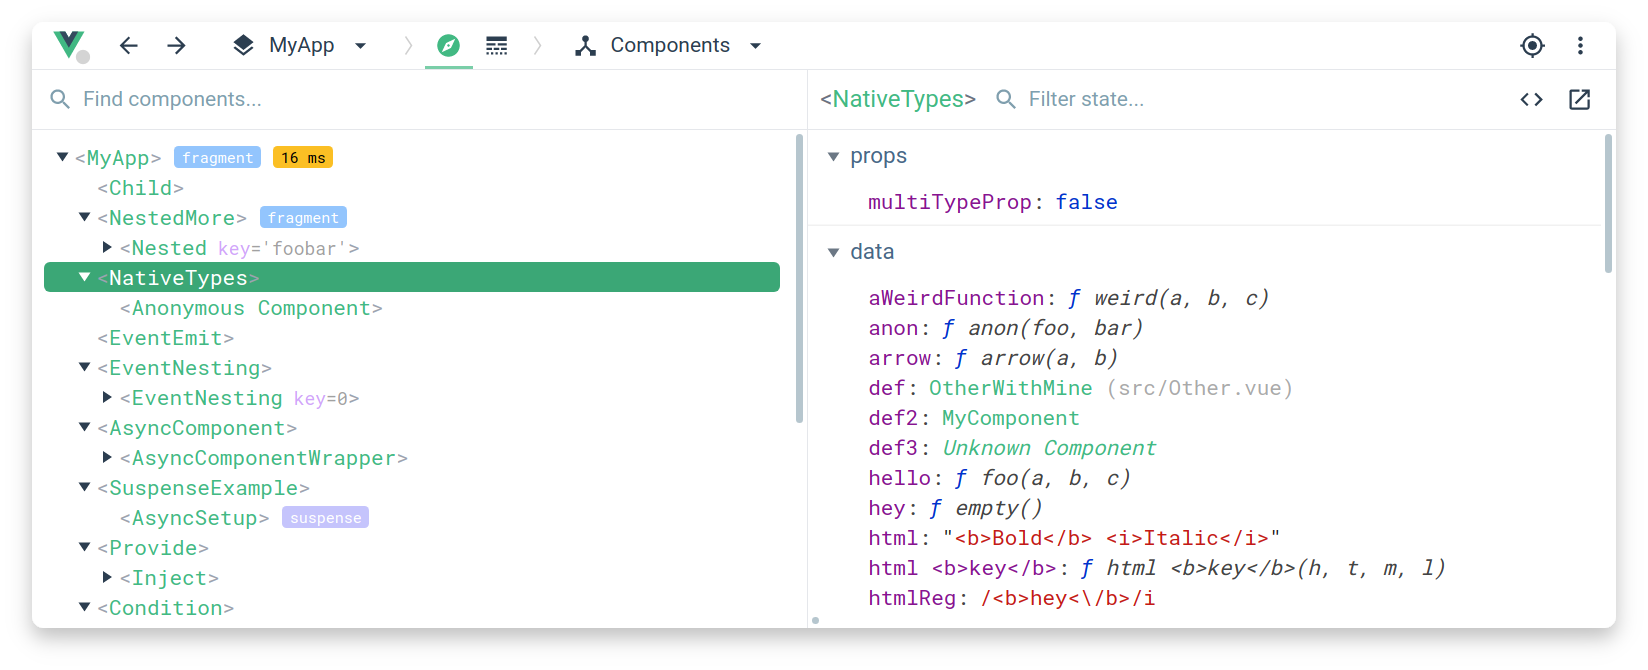
\includegraphics{./img/screenshot-shadow.png} 
\end{center}
    

\columnratio{0.55}
\begin{paracol}{2}
 
\switchcolumn[0]*%%%%%%%
\begin{itemize}
\item
  \href{https://devtools.vuejs.org/}{Documentation}
\item
  \href{https://chrome.google.com/webstore/detail/vuejs-devtools/nhdogjmejiglipccpnnnanhbledajbpd}{Chrome
  Extension}
\item
  \href{https://addons.mozilla.org/en-US/firefox/addon/vue-js-devtools/}{Firefox
  Addon}
\item
  \href{https://microsoftedge.microsoft.com/addons/detail/vuejs-devtools/olofadcdnkkjdfgjcmjaadnlehnnihnl}{Edge
  Extension}
\item
  \href{https://devtools.vuejs.org/guide/installation.html\#standalone}{Standalone
  Electron app}
\end{itemize}
\switchcolumn
\begin{itemize}
\item
  \href{https://devtools.vuejs.org/}{文档}
\item
  \href{https://chrome.google.com/webstore/detail/vuejs-devtools/nhdogjmejiglipccpnnnanhbledajbpd}{Chrome
  扩展商店页}
\item
  \href{https://addons.mozilla.org/en-US/firefox/addon/vue-js-devtools/}{Firefox
  所属插件页}
\item
  \href{https://microsoftedge.microsoft.com/addons/detail/vuejs-devtools/olofadcdnkkjdfgjcmjaadnlehnnihnl}{Edge
  扩展}
\item
  \href{https://devtools.vuejs.org/guide/installation.html\#standalone}{独立的
  Electron 应用所属插件}
\end{itemize}
\end{paracol}

\columnratio{0.55}
\begin{paracol}{2}
 
\switchcolumn[0]*%%%%%%%
\subsection{TypeScript}
\switchcolumn
\subsection{TypeScript}
\switchcolumn[0]*%%%%%%%
Main article:
\href{https://vuejs.org/guide/typescript/overview.html}{Using Vue with
TypeScript}.
\switchcolumn
具体细节请参考章节:\href{https://cn.vuejs.org/guide/typescript/overview.html}{配合
TypeScript 使用 Vue}。
\switchcolumn[0]*%%%%%%%
\begin{itemize}
\item
  \href{https://github.com/johnsoncodehk/volar}{Volar} provides type
  checking for SFCs using
  \texttt{\textless{}script\ lang="ts"\textgreater{}} blocks, including
  template expressions and cross-component props validation.
\item
  Use
  \href{https://github.com/vuejs/language-tools/tree/master/packages/tsc}{\texttt{vue-tsc}}
  for performing the same type checking from the command line, or for
  generating \texttt{d.ts} files for SFCs.
\end{itemize}
\switchcolumn
\begin{itemize}
\item
  \href{https://github.com/johnsoncodehk/volar}{Volar} 插件能够为
  \texttt{\textless{}script\ lang="ts"\textgreater{}}
  块提供类型检查,也能对模板内表达式和组件之间 props
  提供自动补全和类型验证。
\item
  使用
  \href{https://github.com/vuejs/language-tools/tree/master/packages/tsc}{\texttt{vue-tsc}}
  可以在命令行中执行相同的类型检查,通常用来生成单文件组件的
  \texttt{d.ts} 文件。
\end{itemize} 
\switchcolumn[0]*%%%%%%%
\subsection{Testing}
\switchcolumn
\subsection{测试}
\switchcolumn[0]*%%%%%%%
Main article:
\href{https://vuejs.org/guide/scaling-up/testing.html}{Testing Guide}.
\switchcolumn
具体细节请参考章节:\href{https://cn.vuejs.org/guide/scaling-up/testing.html}{测试指南}。
\switchcolumn[0]*%%%%%%%
\begin{itemize}
\item
  \href{https://www.cypress.io/}{Cypress} is recommended for E2E tests.
  It can also be used for component testing for Vue SFCs via the
  \href{https://docs.cypress.io/guides/component-testing/introduction}{Cypress
  Component Test Runner}.
\item
  \href{https://vitest.dev/}{Vitest} is a test runner created by Vue /
  Vite team members that focuses on speed. It is specifically designed
  for Vite-based applications to provide the same instant feedback loop
  for unit / component testing.
\item
  \href{https://jestjs.io/}{Jest} can be made to work with Vite via
  \href{https://github.com/sodatea/vite-jest}{vite-jest}. However, this
  is only recommended if you have existing Jest-based test suites that
  you need to migrate over to a Vite-based setup, as Vitest provides
  similar functionalities with a much more efficient integration.
\end{itemize}
\switchcolumn
\begin{itemize}
\item
  \href{https://www.cypress.io/}{Cypress} 推荐用于 E2E 测试。也可以通过
  \href{https://docs.cypress.io/guides/component-testing/introduction}{Cypress
  组件测试运行器}来给 Vue SFC 作单文件组件测试。
\item
  \href{https://vitest.dev/}{Vitest}
  是一个追求更快运行速度的测试运行器,由 Vue / Vite
  团队成员开发。主要针对基于 Vite
  的应用设计,可以为组件提供即时响应的测试反馈。
\item
  \href{https://jestjs.io/}{Jest} 可以通过
  \href{https://github.com/sodatea/vite-jest}{vite-jest} 配合 Vite
  使用。不过只推荐在你已经有一套基于 Jest 的测试集、且想要迁移到基于
  Vite 的开发配置时使用,因为 Vitest 也能够提供类似的功能,且后者与 Vite
  的集成更方便高效。
\end{itemize}
\switchcolumn[0]*%%%%%%%
\subsection{Linting}
\switchcolumn
\subsection{代码规范}
\switchcolumn[0]*%%%%%%%
The Vue team maintains
\href{https://github.com/vuejs/eslint-plugin-vue}{eslint-plugin-vue}, an
\href{https://eslint.org/}{ESLint} plugin that supports SFC-specific
linting rules.
\switchcolumn
Vue 团队维护着
\href{https://github.com/vuejs/eslint-plugin-vue}{eslint-plugin-vue}
项目,它是一个 \href{https://eslint.org/}{ESLint} 插件,会提供 SFC
相关规则的定义。
\switchcolumn[0]*%%%%%%%
Users previously using Vue CLI may be used to having linters configured
via webpack loaders. However when using a Vite-based build setup, our
general recommendation is:
\switchcolumn
之前使用 Vue CLI 的用户可能习惯于通过 webpack loader
来配置规范检查器。然而,若基于 Vite 构建,我们一般推荐:
\switchcolumn[0]*%%%%%%%
\begin{enumerate}
\item
  \texttt{npm\ install\ -D\ eslint\ eslint-plugin-vue}, then follow
  \texttt{eslint-plugin-vue}'s
  \href{https://eslint.vuejs.org/user-guide/\#usage}{configuration
  guide}.
\item
  Setup ESLint IDE extensions, for example
  \href{https://marketplace.visualstudio.com/items?itemName=dbaeumer.vscode-eslint}{ESLint
  for VSCode}, so you get linter feedback right in your editor during
  development. This also avoids unnecessary linting cost when starting
  the dev server.
\item
  Run ESLint as part of the production build command, so you get full
  linter feedback before shipping to production.
\item
  (Optional) Setup tools like
  \href{https://github.com/okonet/lint-staged}{lint-staged} to
  automatically lint modified files on git commit.
\end{enumerate}
\switchcolumn
\begin{enumerate}
\item
  \texttt{npm\ install\ -D\ eslint\ eslint-plugin-vue},然后遵照
  \texttt{eslint-plugin-vue}
  的\href{https://eslint.vuejs.org/user-guide/\#usage}{指引}进行配置。
\item
  启用 ESLint IDE 插件,比如
  \href{https://marketplace.visualstudio.com/items?itemName=dbaeumer.vscode-eslint}{ESLint
  for
  VSCode},然后你就可以在开发时获得规范检查器的反馈。这同时也避免了启动开发服务器时不必要的规范检查。
\item
  将 ESLint
  格式检查作为一个生产构建的步骤,保证你可以在最终打包时获得完整的规范检查反馈。
\item
  (可选) 启用类似
  \href{https://github.com/okonet/lint-staged}{lint-staged} 一类的工具在
  git commit 提交时自动执行规范检查。
\end{enumerate}
\end{paracol}

\columnratio{0.55}
\begin{paracol}{2}
 
\switchcolumn[0]*%%%%%%%
\subsection{Formatting}
\switchcolumn
\subsection{格式化}
\switchcolumn[0]*%%%%%%%
\begin{itemize}
\item
  The \href{https://github.com/johnsoncodehk/volar}{Volar} VSCode
  extension provides formatting for Vue SFCs out of the box.
\item
  Alternatively, \href{https://prettier.io/}{Prettier} provides built-in
  Vue SFC formatting support.
\end{itemize}
\switchcolumn
\begin{itemize}
\item
  \href{https://github.com/johnsoncodehk/volar}{Volar} VSCode 插件为 Vue
  SFC 提供了开箱即用的格式化功能。
\item
  除此之外,\href{https://prettier.io/}{Prettier} 也提供了内置的 Vue SFC
  格式化支持。
\end{itemize}
\switchcolumn[0]*%%%%%%%
\subsection{SFC Custom Block Integrations}
\switchcolumn
\subsection{SFC 自定义块集成}
\switchcolumn[0]*%%%%%%%
Custom blocks are compiled into imports to the same Vue file with
different request queries. It is up to the underlying build tool to
handle these import requests.
\switchcolumn
自定义块被编译成导入到同一 Vue
文件的不同请求查询。这取决于底层构建工具如何处理这类导入请求。
\switchcolumn[0]*%%%%%%%
\begin{itemize}
\item
  If using Vite, a custom Vite plugin should be used to transform
  matched custom blocks into executable JavaScript.
  \href{https://github.com/vitejs/vite-plugin-vue/tree/main/packages/plugin-vue\#example-for-transforming-custom-blocks}{Example}
\item
  If using Vue CLI or plain webpack, a webpack loader should be
  configured to transform the matched blocks.
  \href{https://vue-loader.vuejs.org/guide/custom-blocks.html}{Example}
\end{itemize}
\switchcolumn
\begin{itemize}
\item
  如果使用 Vite,需使用一个自定义 Vite 插件将自定义块转换为可执行的
  JavaScript
  代码。\href{https://github.com/vitejs/vite-plugin-vue/tree/main/packages/plugin-vue\#example-for-transforming-custom-blocks}{示例}。
\item
  如果使用 Vue CLI 或只是 webpack,需要使用一个 loader
  来配置如何转换匹配到的自定义块。\href{https://vue-loader.vuejs.org/zh/guide/custom-blocks.html}{示例}。
\end{itemize}
\switchcolumn[0]*%%%%%%%
\subsection{Lower-Level Packages}
\switchcolumn
\subsection{底层库}
\switchcolumn[0]*%%%%%%%
\subsubsection{@vue/compiler-sfc}
\switchcolumn
\subsubsection{@vue/compiler-sfc}
\switchcolumn[0]*%%%%%%%
\begin{itemize}
\item
  \href{https://github.com/vuejs/core/tree/main/packages/compiler-sfc}{Docs}
\end{itemize}
\switchcolumn
\begin{itemize}
\item
  \href{https://github.com/vuejs/core/tree/main/packages/compiler-sfc}{文档}
\end{itemize}
\switchcolumn[0]*%%%%%%%
This package is part of the Vue core monorepo and is always published
with the same version as the main \texttt{vue} package. It is included
as a dependency of the main \texttt{vue} package and proxied under
\texttt{vue/compiler-sfc} so you don't need to install it individually.
\switchcolumn
这个包是 Vue 核心 monorepo 的一部分,并始终和 \texttt{vue}
主包版本号保持一致。它已经成为 \texttt{vue} 主包的一个依赖并代理到了
\texttt{vue/compiler-sfc} 目录下,因此你无需单独安装它。
\switchcolumn[0]*%%%%%%%
The package itself provides lower-level utilities for processing Vue
SFCs and is only meant for tooling authors that need to support Vue SFCs
in custom tools.
\switchcolumn
这个包本身提供了处理 Vue SFC 的底层的功能,并只适用于需要支持 Vue SFC
相关工具链的开发者。
\switchcolumn[0]*%%%%%%%
\begin{vueQuote}{TIP}
Always prefer using this package via the \texttt{vue/compiler-sfc} deep
import since this ensures its version is in sync with the Vue runtime.
\end{vueQuote} 
\switchcolumn
\begin{vueQuote}{TIP}
请始终选择通过 \texttt{vue/compiler-sfc}
的深度导入来使用这个包,因为这样可以确保其与 Vue 运行时版本同步。
\end{vueQuote} 
\end{paracol}

\columnratio{0.55}
\begin{paracol}{2}
 
\switchcolumn[0]*%%%%%%%
\subsubsection{@vitejs/plugin-vue}
\switchcolumn
\subsubsection{@vitejs/plugin-vue}
\switchcolumn[0]*%%%%%%%
\begin{itemize}
\item
  \href{https://github.com/vitejs/vite-plugin-vue/tree/main/packages/plugin-vue}{Docs}
\end{itemize}
\switchcolumn
\begin{itemize}
\item
  \href{https://github.com/vitejs/vite-plugin-vue/tree/main/packages/plugin-vue}{文档}
\end{itemize}
\switchcolumn[0]*%%%%%%%
Official plugin that provides Vue SFC support in Vite.
\switchcolumn
为 Vite 提供 Vue SFC 支持的官方插件。
\switchcolumn[0]*%%%%%%%
\subsubsection{vue-loader}
\switchcolumn
\subsubsection{vue-loader}
\switchcolumn[0]*%%%%%%%
\begin{itemize}
\item
  \href{https://vue-loader.vuejs.org/}{Docs}
\end{itemize}
\switchcolumn
\begin{itemize}
\item
  \href{https://vue-loader.vuejs.org/zh/}{文档}
\end{itemize}
\switchcolumn[0]*%%%%%%%
The official loader that provides Vue SFC support in webpack. If you are
using Vue CLI, also see
\href{https://cli.vuejs.org/guide/webpack.html\#modifying-options-of-a-loader}{docs
on modifying \texttt{vue-loader} options in Vue CLI}.
\switchcolumn
为 webpack 提供 Vue SFC 支持的官方 loader。如果你正在使用 Vue
CLI,也可以看看\href{https://cli.vuejs.org/zh/guide/webpack.html\#修改-loader-选项}{如何在
Vue CLI 中更改 \texttt{vue-loader} 选项的文档}。
\switchcolumn[0]*%%%%%%%
\subsection{Other Online Playgrounds}
\switchcolumn
\subsection{其他在线演练场}
\switchcolumn[0]*%%%%%%%
\begin{itemize}
\item
  \href{https://play.vueuse.org/}{VueUse Playground}
\item
  \href{https://replit.com/@templates/VueJS-with-Vite}{Vue + Vite on
  Repl.it}
\item
  \href{https://codesandbox.io/s/vue-3}{Vue on CodeSandbox}
\item
  \href{https://codepen.io/pen/editor/vue}{Vue on Codepen}
\item
  \href{https://components.studio/create/vue3}{Vue on Components.studio}
\item
  \href{https://webcomponents.dev/create/cevue}{Vue on
  WebComponents.dev}
\end{itemize}
\switchcolumn
\begin{itemize}
\item
  \href{https://play.vueuse.org/}{VueUse Playground}
\item
  \href{https://replit.com/@templates/VueJS-with-Vite}{Vue + Vite on
  Repl.it}
\item
  \href{https://codesandbox.io/s/vue-3}{Vue on CodeSandbox}
\item
  \href{https://codepen.io/pen/editor/vue}{Vue on Codepen}
\item
  \href{https://components.studio/create/vue3}{Vue on Components.studio}
\item
  \href{https://webcomponents.dev/create/cevue}{Vue on
  WebComponents.dev}
\end{itemize}
\end{paracol}
 %todo 看

\columnratio{0.55}
\begin{paracol}{2}
 
\switchcolumn[0]*%%%%%%%
\section{Routing}
\switchcolumn
\section{路由}
\switchcolumn[0]*%%%%%%%
\subsection{Client-Side vs. Server-Side Routing}
\switchcolumn
\subsection{客户端 vs. 服务端路由}
\switchcolumn[0]*%%%%%%%
Routing on the server side means the server sending a response based on
the URL path that the user is visiting. When we click on a link in a
traditional server-rendered web app, the browser receives an HTML
response from the server and reloads the entire page with the new HTML.
\switchcolumn
服务端路由指的是服务器根据用户访问的 URL
路径返回不同的响应结果。当我们在一个传统的服务端渲染的 web
应用中点击一个链接时,浏览器会从服务端获得全新的
HTML,然后重新加载整个页面。
\switchcolumn[0]*%%%%%%%
In a
\href{https://developer.mozilla.org/en-US/docs/Glossary/SPA}{Single-Page
Application} (SPA), however, the client-side JavaScript can intercept
the navigation, dynamically fetch new data, and update the current page
without full page reloads. This typically results in a more snappy user
experience, especially for use cases that are more like actual
"applications", where the user is expected to perform many interactions
over a long period of time.
\switchcolumn
然而,在\href{https://developer.mozilla.org/en-US/docs/Glossary/SPA}{单页面应用}中,客户端的
JavaScript
可以拦截页面的跳转请求,动态获取新的数据,然后在无需重新加载的情况下更新当前页面。这样通常可以带来更顺滑的用户体验,尤其是在更偏向``应用''的场景下,因为这类场景下用户通常会在很长的一段时间中做出多次交互。
\switchcolumn[0]*%%%%%%%
In such SPAs, the "routing" is done on the client side, in the browser.
A client-side router is responsible for managing the application's
rendered view using browser APIs such as
\href{https://developer.mozilla.org/en-US/docs/Web/API/History}{History
API} or the
\href{https://developer.mozilla.org/en-US/docs/Web/API/Window/hashchange_event}{\texttt{hashchange}
event}.
\switchcolumn
在这类单页应用中,``路由''是在客户端执行的。一个客户端路由器的职责就是利用诸如
\href{https://developer.mozilla.org/en-US/docs/Web/API/History}{History
API} 或是
\href{https://developer.mozilla.org/en-US/docs/Web/API/Window/hashchange_event}{\texttt{hashchange}
事件}这样的浏览器 API 来管理应用当前应该渲染的视图。
\end{paracol}

\columnratio{0.55}
\begin{paracol}{2}
 
\switchcolumn[0]*%%%%%%%
\subsection{Official Router}
\switchcolumn
\subsection{官方路由}
\switchcolumn[0]*%%%%%%%
\href{https://vueschool.io/courses/vue-router-4-for-everyone?friend=vuejs}{Watch
a Free Video Course on Vue School}
\switchcolumn
在 Vue School 上观看免费的视频课程
\switchcolumn[0]*%%%%%%%
Vue is well-suited for building SPAs. For most SPAs, it's recommended to
use the officially-supported \href{https://github.com/vuejs/router}{Vue
Router library}. For more details, see Vue Router's
\href{https://router.vuejs.org/}{documentation}.
\switchcolumn
Vue
很适合用来构建单页面应用。对于大多数此类应用,都推荐使用官方支持的\href{https://github.com/vuejs/router}{路由库}。要了解更多细节,请查看
\href{https://router.vuejs.org/zh/}{Vue Router 的文档}。
\end{paracol}

\columnratio{0.55}
\begin{paracol}{2}
 
\switchcolumn[0]*%%%%%%%
\subsection{Simple Routing from Scratch}
\switchcolumn
\subsection{从头开始实现一个简单的路由}
\switchcolumn[0]*%%%%%%%
If you only need very simple routing and do not wish to involve a
full-featured router library, you can do so with
\href{https://vuejs.org/guide/essentials/component-basics.html\#dynamic-components}{Dynamic
Components} and update the current component state by listening to
browser
\href{https://developer.mozilla.org/en-US/docs/Web/API/Window/hashchange_event}{\texttt{hashchange}
events} or using the
\href{https://developer.mozilla.org/en-US/docs/Web/API/History}{History
API}.
\switchcolumn
如果你只需要一个简单的页面路由,而不想为此引入一整个路由库,你可以通过\href{https://cn.vuejs.org/guide/essentials/component-basics.html\#dynamic-components}{动态组件}的方式,监听浏览器
\href{https://developer.mozilla.org/en-US/docs/Web/API/Window/hashchange_event}{\texttt{hashchange}
事件}或使用
\href{https://developer.mozilla.org/en-US/docs/Web/API/History}{History
API} 来更新当前组件。
\switchcolumn[0]*%%%%%%%
Here's a bare-bone example:
\switchcolumn
下面是一个简单的例子:
\switchcolumn[0]*%%%%%%%
\begin{codeHtml}
<script setup>
import { ref, computed } from 'vue'
import Home from './Home.vue'
import About from './About.vue'
import NotFound from './NotFound.vue'
const routes = {
  '/': Home,
  '/about': About
}
const currentPath = ref(window.location.hash)
window.addEventListener('hashchange', () => {
  currentPath.value = window.location.hash
})
const currentView = computed(() => {
  return routes[currentPath.value.slice(1) || '/'] || NotFound
})
</script>
<template>
  <a href="#/">Home</a> |
  <a href="#/about">About</a> |
  <a href="#/non-existent-path">Broken Link</a>
  <component :is="currentView" />
</template>
\end{codeHtml}
\switchcolumn
\begin{codeHtml}
<script setup>
import { ref, computed } from 'vue'
import Home from './Home.vue'
import About from './About.vue'
import NotFound from './NotFound.vue'
const routes = {
  '/': Home,
  '/about': About
}
const currentPath = ref(window.location.hash)
window.addEventListener('hashchange', () => {
  currentPath.value = window.location.hash
})
const currentView = computed(() => {
  return routes[currentPath.value.slice(1) || '/'] || NotFound
})
</script>
<template>
  <a href="#/">Home</a> |
  <a href="#/about">About</a> |
  <a href="#/non-existent-path">Broken Link</a>
  <component :is="currentView" />
</template>
\end{codeHtml}
\switchcolumn[0]*%%%%%%%
\href{https://play.vuejs.org/\#eNptUk1vgkAQ/SsTegAThZp4MmhikzY9mKanXkoPWxjLRpgly6JN1P/eWb5Eywlm572ZN2/m5GyKwj9U6CydsIy1LAyUaKpiHZHMC6UNnEDjbgqxyovKYAIX2GmVg8sktwe9qhzbdz+wga15TW++VWX6fB3dAt6UeVEVJT2me2hhEcWKSgOamVjCCk4RAbiBu6xbT5tI2ML8VDeI6HLlxZXWSOZdmJTJPJB3lJSoo5+pWBipyE9FmU4soU2IJHk+MGUrS4OE2nMtIk4F/aA7BW8Cq3WjYlDbP4isQu4wVp0F1Q1uFH1IPDK+c9cb1NW8B03tyJ//uvhlJmP05hM4n60TX/bb2db0CoNmpbxMDgzmRSYMcgQQCkjZhlXkPASRs7YmhoFYw/k+WXvKiNrTcQgpmuFv7ZOZFSyQ4U9a7ZFgK2lvSTXFDqmIQbCUJTMHFkQOBAwKg16kM3W6O7K3eSs+nbeK+eee1V/XKK0dY4Q3vLhR6uJxMUK8/AFKaB6k}{Try
it in the Playground}
\switchcolumn
\href{https://play.vuejs.org/\#eNptUk1vgkAQ/SsTegAThZp4MmhikzY9mKanXkoPWxjLRpgly6JN1P/eWb5Eywlm572ZN2/m5GyKwj9U6CydsIy1LAyUaKpiHZHMC6UNnEDjbgqxyovKYAIX2GmVg8sktwe9qhzbdz+wga15TW++VWX6fB3dAt6UeVEVJT2me2hhEcWKSgOamVjCCk4RAbiBu6xbT5tI2ML8VDeI6HLlxZXWSOZdmJTJPJB3lJSoo5+pWBipyE9FmU4soU2IJHk+MGUrS4OE2nMtIk4F/aA7BW8Cq3WjYlDbP4isQu4wVp0F1Q1uFH1IPDK+c9cb1NW8B03tyJ//uvhlJmP05hM4n60TX/bb2db0CoNmpbxMDgzmRSYMcgQQCkjZhlXkPASRs7YmhoFYw/k+WXvKiNrTcQgpmuFv7ZOZFSyQ4U9a7ZFgK2lvSTXFDqmIQbCUJTMHFkQOBAwKg16kM3W6O7K3eSs+nbeK+eee1V/XKK0dY4Q3vLhR6uJxMUK8/AFKaB6k}{在演练场中尝试一下}
\end{paracol}


 %todo 看
\columnratio{0.55}
\begin{paracol}{2}
 
\switchcolumn[0]*%%%%%%%
\section{State Management}
\switchcolumn
\section{状态管理}
\switchcolumn[0]*%%%%%%%
\subsection{What is State Management?}
\switchcolumn
\subsection{什么是状态管理?}
\switchcolumn[0]*%%%%%%%
Technically, every Vue component instance already "manages" its own
reactive state. Take a simple counter component as an example:
\switchcolumn
理论上来说,每一个 Vue
组件实例都已经在``管理''它自己的响应式状态了。我们以一个简单的计数器组件为例:
\switchcolumn[0]*%%%%%%%
\begin{codeHtml}
<script setup>
import { ref } from 'vue'
// 状态
const count = ref(0)
// 动作
function increment() {
  count.value++
}
</script>
<!-- 视图 -->
<template>{{ count }}</template>
\end{codeHtml}
\switchcolumn
\begin{codeHtml}
<script setup>
import { ref } from 'vue'
// 状态
const count = ref(0)
// 动作
function increment() {
  count.value++
}
</script>
<!-- 视图 -->
<template>{{ count }}</template>
\end{codeHtml}
\switchcolumn[0]*%%%%%%%
It is a self-contained unit with the following parts:
\switchcolumn
它是一个独立的单元,由以下几个部分组成:
\switchcolumn[0]*%%%%%%%
\begin{itemize}
\item
  The \textbf{state}, the source of truth that drives our app;
\item
  The \textbf{view}, a declarative mapping of the \textbf{state};
\item
  The \textbf{actions}, the possible ways the state could change in
  reaction to user inputs from the \textbf{view}.
\end{itemize}
\switchcolumn
\begin{itemize}
\item
  \textbf{状态}:驱动整个应用的数据源;
\item
  \textbf{视图}:对\textbf{状态}的一种声明式映射;
\item
  \textbf{交互}:状态根据用户在\textbf{视图}中的输入而作出相应变更的可能方式。
\end{itemize}
\switchcolumn[0]*%%%%%%%
This is a simple representation of the concept of "one-way data flow":
\switchcolumn
下面是``单向数据流''这一概念的简单图示:
\end{paracol}

\begin{center} 
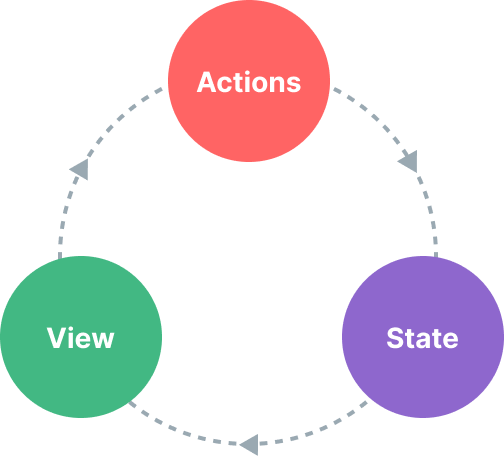
\includegraphics{./img/state-flow.a8bc738e.png} 
\end{center}
    

\columnratio{0.55}
\begin{paracol}{2}
 
\switchcolumn[0]*%%%%%%%
However, the simplicity starts to break down when we have
\textbf{multiple components that share a common state}:
\switchcolumn
然而,当我们有\textbf{多个组件共享一个共同的状态}时,就没有这么简单了:
\switchcolumn[0]*%%%%%%%
\begin{enumerate}
\item
  Multiple views may depend on the same piece of state.
\item
  Actions from different views may need to mutate the same piece of
  state.
\end{enumerate}
\switchcolumn
\begin{enumerate}
\item
  多个视图可能都依赖于同一份状态。
\item
  来自不同视图的交互也可能需要更改同一份状态。
\end{enumerate}
\switchcolumn[0]*%%%%%%%
For case one, a possible workaround is by "lifting" the shared state up
to a common ancestor component, and then pass it down as props. However,
this quickly gets tedious in component trees with deep hierarchies,
leading to another problem known as
\href{https://vuejs.org/guide/components/provide-inject.html\#prop-drilling}{Prop
Drilling}.
\switchcolumn
对于情景
1,一个可行的办法是将共享状态``提升''到共同的祖先组件上去,再通过 props
传递下来。然而在深层次的组件树结构中这么做的话,很快就会使得代码变得繁琐冗长。这会导致另一个问题:\href{https://cn.vuejs.org/guide/components/provide-inject.html\#prop-drilling}{Prop
逐级透传问题}。
\switchcolumn[0]*%%%%%%%
For case two, we often find ourselves resorting to solutions such as
reaching for direct parent / child instances via template refs, or
trying to mutate and synchronize multiple copies of the state via
emitted events. Both of these patterns are brittle and quickly lead to
unmaintainable code.
\switchcolumn
对于情景
2,我们经常发现自己会直接通过模板引用获取父/子实例,或者通过触发的事件尝试改变和同步多个状态的副本。但这些模式的健壮性都不甚理想,很容易就会导致代码难以维护。
\switchcolumn[0]*%%%%%%%
A simpler and more straightforward solution is to extract the shared
state out of the components, and manage it in a global singleton. With
this, our component tree becomes a big "view", and any component can
access the state or trigger actions, no matter where they are in the
tree!
\switchcolumn
一个更简单直接的解决方案是抽取出组件间的共享状态,放在一个全局单例中来管理。这样我们的组件树就变成了一个大的``视图'',而任何位置上的组件都可以访问其中的状态或触发动作。
\switchcolumn[0]*%%%%%%%
\subsection{Simple State Management with Reactivity API}
\switchcolumn
\subsection{用响应式 API 做简单状态管理}
\switchcolumn[0]*%%%%%%%
If you have a piece of state that should be shared by multiple
instances, you can use
\href{https://vuejs.org/api/reactivity-core.html\#reactive}{\texttt{reactive()}}
to create a reactive object, and then import it into multiple
components:
\switchcolumn
如果你有一部分状态需要在多个组件实例间共享,你可以使用
\href{https://cn.vuejs.org/api/reactivity-core.html\#reactive}{\texttt{reactive()}}
来创建一个响应式对象,并将它导入到多个组件中:
\switchcolumn[0]*%%%%%%%
\begin{codeJs}
// store.js
import { reactive } from 'vue'
export const store = reactive({
  count: 0
})
\end{codeJs}
\switchcolumn
\begin{codeJs}
// store.js
import { reactive } from 'vue'
export const store = reactive({
  count: 0
})
\end{codeJs}
\switchcolumn[0]*%%%%%%%
\begin{codeHtml}
<!-- ComponentA.vue -->
<script setup>
import { store } from './store.js'
</script>
<template>From A: {{ store.count }}</template>
\end{codeHtml}
\switchcolumn
\begin{codeHtml}
<!-- ComponentA.vue -->
<script setup>
import { store } from './store.js'
</script>
<template>From A: {{ store.count }}</template>
\end{codeHtml}
\switchcolumn[0]*%%%%%%%
\begin{codeHtml}
<!-- ComponentB.vue -->
<script setup>
import { store } from './store.js'
</script>
<template>From B: {{ store.count }}</template>
\end{codeHtml}
\switchcolumn
\begin{codeHtml}
<!-- ComponentB.vue -->
<script setup>
import { store } from './store.js'
</script>
<template>From B: {{ store.count }}</template>
\end{codeHtml}
\switchcolumn[0]*%%%%%%%
Now whenever the \texttt{store} object is mutated, both
\texttt{\textless{}ComponentA\textgreater{}} and
\texttt{\textless{}ComponentB\textgreater{}} will update their views
automatically - we have a single source of truth now.
\switchcolumn
现在每当 \texttt{store}
对象被更改时,\texttt{\textless{}ComponentA\textgreater{}} 与
\texttt{\textless{}ComponentB\textgreater{}}
都会自动更新它们的视图。现在我们有了单一的数据源。
\switchcolumn[0]*%%%%%%%
However, this also means any component importing \texttt{store} can
mutate it however they want:
\switchcolumn
然而,这也意味着任意一个导入了 \texttt{store}
的组件都可以随意修改它的状态:
\switchcolumn[0]*%%%%%%%
\begin{codeHtml}
<template>
  <button @click="store.count++">
    From B: {{ store.count }}
  </button>
</template>
\end{codeHtml}
\switchcolumn
\begin{codeHtml}
<template>
  <button @click="store.count++">
    From B: {{ store.count }}
  </button>
</template>
\end{codeHtml}
\switchcolumn[0]*%%%%%%%
While this works in simple cases, global state that can be arbitrarily
mutated by any component is not going to be very maintainable in the
long run. To ensure the state-mutating logic is centralized like the
state itself, it is recommended to define methods on the store with
names that express the intention of the actions:
\switchcolumn
虽然这在简单的情况下是可行的,但从长远来看,可以被任何组件任意改变的全局状态是不太容易维护的。为了确保改变状态的逻辑像状态本身一样集中,建议在
store 上定义方法,方法的名称应该要能表达出行动的意图:
\switchcolumn[0]*%%%%%%%
\begin{codeJs}
// store.js
import { reactive } from 'vue'
export const store = reactive({
  count: 0,
  increment() {
    this.count++
  }
})
\end{codeJs}
\switchcolumn
\begin{codeJs}
// store.js
import { reactive } from 'vue'
export const store = reactive({
  count: 0,
  increment() {
    this.count++
  }
})
\end{codeJs}
\switchcolumn[0]*%%%%%%%
\begin{codeHtml}
<template>
  <button @click="store.increment()">
    From B: {{ store.count }}
  </button>
</template>
\end{codeHtml}
\switchcolumn
\begin{codeHtml}
<template>
  <button @click="store.increment()">
    From B: {{ store.count }}
  </button>
</template>
\end{codeHtml}
\switchcolumn[0]*%%%%%%%
\href{https://play.vuejs.org/\#eNrNkk1uwyAQha8yYpNEiUzXllPVrtRTeJNSqtLGgGBsVbK4ewdwnT9FWWSTFczwmPc+xMhqa4uhl6xklRdOWQQvsbfPrVadNQ7h1dCqpcYaPp3pYFHwQyteXVxKm0tpM0krnm3IgAqUnd3vUFIFUB1Z8bNOkzoVny+wDTuNcZ1gBI/GSQhzqlQX3/5Gng81pA1t33tEo+FF7JX42bYsT1BaONlRguWqZZMU4C261CWMk3EhTK8RQphm8Twse/BscoUsvdqDkTX3kP3nI6aZwcmdQDUcMPJPabX8TQphtCf0RLqd1csxuqQAJTxtYnEUGtIpAH4pn1Ou17FDScOKhT+QNAVM}{Try
it in the Playground}
\switchcolumn
\href{https://play.vuejs.org/\#eNrNkk1uwyAQha8yYpNEiUzXllPVrtRTeJNSqtLGgGBsVbK4ewdwnT9FWWSTFczwmPc+xMhqa4uhl6xklRdOWQQvsbfPrVadNQ7h1dCqpcYaPp3pYFHwQyteXVxKm0tpM0krnm3IgAqUnd3vUFIFUB1Z8bNOkzoVny+wDTuNcZ1gBI/GSQhzqlQX3/5Gng81pA1t33tEo+FF7JX42bYsT1BaONlRguWqZZMU4C261CWMk3EhTK8RQphm8Twse/BscoUsvdqDkTX3kP3nI6aZwcmdQDUcMPJPabX8TQphtCf0RLqd1csxuqQAJTxtYnEUGtIpAH4pn1Ou17FDScOKhT+QNAVM}{在演练场中尝试一下}
\switchcolumn[0]*%%%%%%%
\begin{vueQuote}{TIP}
Note the click handler uses \texttt{store.increment()} with parentheses
- this is necessary to call the method with the proper \texttt{this}
context since it's not a component method.
\end{vueQuote} 
\switchcolumn
\begin{vueQuote}{TIP}
请注意这里点击的处理函数使用了
\texttt{store.increment()},带上了圆括号作为内联表达式调用,因为它并不是组件的方法,并且必须要以正确的
\texttt{this} 上下文来调用。
\end{vueQuote} 
\switchcolumn[0]*%%%%%%%
Although here we are using a single reactive object as a store, you can
also share reactive state created using other
\href{https://vuejs.org/api/reactivity-core.html}{Reactivity APIs} such
as \texttt{ref()} or \texttt{computed()}, or even return global state
from a
\href{https://vuejs.org/guide/reusability/composables.html}{Composable}:
\switchcolumn
除了我们这里用到的单个响应式对象作为一个 store
之外,你还可以使用其他\href{https://cn.vuejs.org/api/reactivity-core.html}{响应式
API} 例如 \texttt{ref()} 或是
\texttt{computed()},或是甚至通过一个\href{https://cn.vuejs.org/guide/reusability/composables.html}{组合式函数}来返回一个全局状态:
\switchcolumn[0]*%%%%%%%
\begin{codeJs}
import { ref } from 'vue'
// 全局状态,创建在模块作用域下
const globalCount = ref(1)
export function useCount() {
  // 局部状态,每个组件都会创建
  const localCount = ref(1)
  return {
    globalCount,
    localCount
  }
}
\end{codeJs}
\switchcolumn
\begin{codeJs}
import { ref } from 'vue'
// 全局状态,创建在模块作用域下
const globalCount = ref(1)
export function useCount() {
  // 局部状态,每个组件都会创建
  const localCount = ref(1)
  return {
    globalCount,
    localCount
  }
}
\end{codeJs}
\switchcolumn[0]*%%%%%%%
The fact that Vue's reactivity system is decoupled from the component
model makes it extremely flexible.
\switchcolumn
事实上,Vue 的响应性系统与组件层是解耦的,这使得它非常灵活。
\end{paracol}

\columnratio{0.55}
\begin{paracol}{2}
 
\switchcolumn[0]*%%%%%%%
\subsection{SSR Considerations}
\switchcolumn
\subsection{SSR 相关细节}
\switchcolumn[0]*%%%%%%%
If you are building an application that leverages
\href{https://vuejs.org/guide/scaling-up/ssr.html}{Server-Side Rendering
(SSR)}, the above pattern can lead to issues due to the store being a
singleton shared across multiple requests. This is discussed in
\href{https://vuejs.org/guide/scaling-up/ssr.html\#cross-request-state-pollution}{more
details} in the SSR guide.
\switchcolumn
如果你正在构建一个需要利用\href{https://cn.vuejs.org/guide/scaling-up/ssr.html}{服务端渲染
(SSR)} 的应用,由于 store
是跨多个请求共享的单例,上述模式可能会导致问题。这在 SSR
指引那一章节会讨论\href{https://cn.vuejs.org/guide/scaling-up/ssr.html\#cross-request-state-pollution}{更多细节}。
\switchcolumn[0]*%%%%%%%
\subsection{Pinia}
\switchcolumn
\subsection{Pinia}
\switchcolumn[0]*%%%%%%%
While our hand-rolled state management solution will suffice in simple
scenarios, there are many more things to consider in large-scale
production applications:
\switchcolumn
虽然我们的手动状态管理解决方案在简单的场景中已经足够了,但是在大规模的生产应用中还有很多其他事项需要考虑:
\switchcolumn[0]*%%%%%%%
\begin{itemize}
\item
  Stronger conventions for team collaboration
\item
  Integrating with the Vue DevTools, including timeline, in-component
  inspection, and time-travel debugging
\item
  Hot Module Replacement
\item
  Server-Side Rendering support
\end{itemize}
\switchcolumn
\begin{itemize}
\item
  更强的团队协作约定
\item
  与 Vue DevTools 集成,包括时间轴、组件内部审查和时间旅行调试
\item
  模块热更新 (HMR)
\item
  服务端渲染支持
\end{itemize}
\switchcolumn[0]*%%%%%%%
\href{https://pinia.vuejs.org/}{Pinia} is a state management library
that implements all of the above. It is maintained by the Vue core team,
and works with both Vue 2 and Vue 3.
\switchcolumn
\href{https://pinia.vuejs.org/zh/}{Pinia}
就是一个实现了上述需求的状态管理库,由 Vue 核心团队维护,对 Vue 2 和 Vue
3 都可用。
\switchcolumn[0]*%%%%%%%
Existing users may be familiar with
\href{https://vuex.vuejs.org/}{Vuex}, the previous official state
management library for Vue. With Pinia serving the same role in the
ecosystem, Vuex is now in maintenance mode. It still works, but will no
longer receive new features. It is recommended to use Pinia for new
applications.
\switchcolumn
现有用户可能对 \href{https://vuex.vuejs.org/zh/}{Vuex} 更熟悉,它是 Vue
之前的官方状态管理库。由于 Pinia
在生态系统中能够承担相同的职责且能做得更好,因此 Vuex
现在处于维护模式。它仍然可以工作,但不再接受新的功能。对于新的应用,建议使用
Pinia。
\switchcolumn[0]*%%%%%%%
Pinia started out as an exploration of what the next iteration of Vuex
could look like, incorporating many ideas from core team discussions for
Vuex 5. Eventually, we realized that Pinia already implements most of
what we wanted in Vuex 5, and decided to make it the new recommendation
instead.
\switchcolumn
事实上,Pinia 最初正是为了探索 Vuex
的下一个版本而开发的,因此整合了核心团队关于 Vuex 5
的许多想法。最终,我们意识到 Pinia 已经实现了我们想要在 Vuex 5
中提供的大部分内容,因此决定将其作为新的官方推荐。
\switchcolumn[0]*%%%%%%%
Compared to Vuex, Pinia provides a simpler API with less ceremony,
offers Composition-API-style APIs, and most importantly, has solid type
inference support when used with TypeScript.
\switchcolumn
相比于 Vuex,Pinia 提供了更简洁直接的 API,并提供了组合式风格的
API,最重要的是,在使用 TypeScript 时它提供了更完善的类型推导。
\end{paracol}

%todo 看

\columnratio{0.55}
\begin{paracol}{2}
 
\switchcolumn[0]*%%%%%%%
\section{Testing}
\switchcolumn
\section{测试}
\switchcolumn[0]*%%%%%%%
\subsection{Why Test?}
\switchcolumn
\subsection{为什么需要测试}
\switchcolumn[0]*%%%%%%%
Automated tests help you and your team build complex Vue applications
quickly and confidently by preventing regressions and encouraging you to
break apart your application into testable functions, modules, classes,
and components. As with any application, your new Vue app can break in
many ways, and it's important that you can catch these issues and fix
them before releasing.
\switchcolumn
自动化测试能够预防无意引入的
bug,并鼓励开发者将应用分解为可测试、可维护的函数、模块、类和组件。这能够帮助你和你的团队更快速、自信地构建复杂的
Vue 应用。与任何应用一样,新的 Vue
应用可能会以多种方式崩溃,因此,在发布前发现并解决这些问题就变得十分重要。
\switchcolumn[0]*%%%%%%%
In this guide, we'll cover basic terminology and provide our
recommendations on which tools to choose for your Vue 3 application.
\switchcolumn
在本篇指引中,我们将介绍一些基本术语,并就你的 Vue 3
应用应选择哪些工具提供一些建议。
\switchcolumn[0]*%%%%%%%
There is one Vue-specific section covering composables. See
\href{https://vuejs.org/guide/scaling-up/testing.html\#testing-composables}{Testing
Composables} below for more details.
\switchcolumn
还有一个特定用于 Vue
的小节,介绍了组合式函数的测试,详情请参阅\href{https://cn.vuejs.org/guide/scaling-up/testing.html\#testing-composables}{测试组合式函数}。
\switchcolumn[0]*%%%%%%%
\subsection{When to Test}
\switchcolumn
\subsection{何时测试}
\switchcolumn[0]*%%%%%%%
Start testing early! We recommend you begin writing tests as soon as you
can. The longer you wait to add tests to your application, the more
dependencies your application will have, and the harder it will be to
start.
\switchcolumn
越早越好!我们建议你尽快开始编写测试。拖得越久,应用就会有越多的依赖和复杂性,想要开始添加测试也就越困难。
\switchcolumn[0]*%%%%%%%
\subsection{Testing Types}
\switchcolumn
\subsection{测试的类型}
\switchcolumn[0]*%%%%%%%
When designing your Vue application's testing strategy, you should
leverage the following testing types:
\switchcolumn
当设计你的 Vue 应用的测试策略时,你应该利用以下几种测试类型:
\switchcolumn[0]*%%%%%%%
\begin{itemize}
\item
  \textbf{Unit}: Checks that inputs to a given function, class, or
  composable are producing the expected output or side effects.
\item
  \textbf{Component}: Checks that your component mounts, renders, can be
  interacted with, and behaves as expected. These tests import more code
  than unit tests, are more complex, and require more time to execute.
\item
  \textbf{End-to-end}: Checks features that span multiple pages and
  makes real network requests against your production-built Vue
  application. These tests often involve standing up a database or other
  backend.
\end{itemize}
\switchcolumn
\begin{itemize}
\item
  \textbf{单元测试}:检查给定函数、类或组合式函数的输入是否产生预期的输出或副作用。
\item
  \textbf{组件测试}:检查你的组件是否正常挂载和渲染、是否可以与之互动,以及表现是否符合预期。这些测试比单元测试导入了更多的代码,更复杂,需要更多时间来执行。
\item
  \textbf{端到端测试}:检查跨越多个页面的功能,并对生产构建的 Vue
  应用进行实际的网络请求。这些测试通常涉及到建立一个数据库或其他后端。
\end{itemize}
\switchcolumn[0]*%%%%%%%
Each testing type plays a role in your application's testing strategy,
and each will protect you against different types of issues.
\switchcolumn
每种测试类型在你的应用的测试策略中都发挥着作用,保护你免受不同类型的问题的影响。
\switchcolumn[0]*%%%%%%%
\subsection{Overview}
\switchcolumn
\subsection{总览}
\switchcolumn[0]*%%%%%%%
We will briefly discuss what each of these are, how they can be
implemented for Vue applications, and provide some general
recommendations.
\switchcolumn
我们将简要地讨论这些测试是什么,以及如何在 Vue
应用中实现它们,并提供一些普适性建议。
\switchcolumn[0]*%%%%%%%
\subsection{Unit Testing}
\switchcolumn
\subsection{单元测试}
\switchcolumn[0]*%%%%%%%
Unit tests are written to verify that small, isolated units of code are
working as expected. A unit test usually covers a single function,
class, composable, or module. Unit tests focus on logical correctness
and only concern themselves with a small portion of the application's
overall functionality. They may mock large parts of your application's
environment (e.g. initial state, complex classes, 3rd party modules, and
network requests).
\switchcolumn
编写单元测试是为了验证小的、独立的代码单元是否按预期工作。一个单元测试通常覆盖一个单个函数、类、组合式函数或模块。单元测试侧重于逻辑上的正确性,只关注应用整体功能的一小部分。他们可能会模拟你的应用环境的很大一部分(如初始状态、复杂的类、第三方模块和网络请求)。
\switchcolumn[0]*%%%%%%%
In general, unit tests will catch issues with a function's business
logic and logical correctness.
\switchcolumn
一般来说,单元测试将捕获函数的业务逻辑和逻辑正确性的问题。
\switchcolumn[0]*%%%%%%%
Take for example this \texttt{increment} function:
\switchcolumn
以这个 \texttt{increment} 函数为例:
\switchcolumn[0]*%%%%%%%
\begin{codeJs}
// helpers.js
export function increment (current, max = 10) {
  if (current < max) {
    return current + 1
  }
  return current
}
\end{codeJs}
\switchcolumn
\begin{codeJs}
// helpers.js
export function increment (current, max = 10) {
  if (current < max) {
    return current + 1
  }
  return current
}
\end{codeJs}
\switchcolumn[0]*%%%%%%%
Because it's very self-contained, it'll be easy to invoke the increment
function and assert that it returns what it's supposed to, so we'll
write a Unit Test.
\switchcolumn
因为它很独立,可以很容易地调用 \texttt{increment}
函数并断言它是否返回了所期望的内容,所以我们将编写一个单元测试。
\switchcolumn[0]*%%%%%%%
If any of these assertions fail, it's clear that the issue is contained
within the \texttt{increment} function.
\switchcolumn
如果任何一条断言失败了,那么问题一定是出在 \texttt{increment} 函数上。
\switchcolumn[0]*%%%%%%%
\begin{codeJs}
// helpers.spec.js
import { increment } from './helpers'
describe('increment', () => {
  test('increments the current number by 1', () => {
    expect(increment(0, 10)).toBe(1)
  })
  test('does not increment the current number over the max', () => {
    expect(increment(10, 10)).toBe(10)
  })
  test('has a default max of 10', () => {
    expect(increment(10)).toBe(10)
  })
})
\end{codeJs}
\switchcolumn
\begin{codeJs}
// helpers.spec.js
import { increment } from './helpers'
describe('increment', () => {
  test('increments the current number by 1', () => {
    expect(increment(0, 10)).toBe(1)
  })
  test('does not increment the current number over the max', () => {
    expect(increment(10, 10)).toBe(10)
  })
  test('has a default max of 10', () => {
    expect(increment(10)).toBe(10)
  })
})
\end{codeJs}
\switchcolumn[0]*%%%%%%%
As mentioned previously, unit testing is typically applied to
self-contained business logic, components, classes, modules, or
functions that do not involve UI rendering, network requests, or other
environmental concerns.
\switchcolumn
如前所述,单元测试通常适用于独立的业务逻辑、组件、类、模块或函数,不涉及
UI 渲染、网络请求或其他环境问题。
\switchcolumn[0]*%%%%%%%
These are typically plain JavaScript / TypeScript modules unrelated to
Vue. In general, writing unit tests for business logic in Vue
applications does not differ significantly from applications using other
frameworks.
\switchcolumn
这些通常是与 Vue 无关的纯 JavaScript/TypeScript 模块。一般来说,在 Vue
应用中为业务逻辑编写单元测试与使用其他框架的应用没有明显区别。
\switchcolumn[0]*%%%%%%%
There are two instances where you DO unit test Vue-specific features:
\switchcolumn
但有两种情况,你必须对 Vue 的特定功能进行单元测试:
\switchcolumn[0]*%%%%%%%
\begin{enumerate}
\item
  Composables
\item
  Components
\end{enumerate}
\switchcolumn
\begin{enumerate}
\item
  组合式函数
\item
  组件
\end{enumerate}
\switchcolumn[0]*%%%%%%%
\subsubsection{Composables}
\switchcolumn
\subsubsection{组合式函数}
\switchcolumn[0]*%%%%%%%
One category of functions specific to Vue applications is
\href{https://vuejs.org/guide/reusability/composables.html}{Composables},
which may require special handling during tests. See
\href{https://vuejs.org/guide/scaling-up/testing.html\#testing-composables}{Testing
Composables} below for more details.
\switchcolumn
有一类 Vue 应用中特有的函数被称为
\href{https://cn.vuejs.org/guide/reusability/composables.html}{组合式函数},在测试过程中可能需要特殊处理。
你可以跳转到下方查看
\href{https://cn.vuejs.org/guide/scaling-up/testing.html\#testing-composables}{测试组合式函数}
了解更多细节。
\end{paracol}

\columnratio{0.55}
\begin{paracol}{2}
\switchcolumn[0]*%%%%%%%
\subsubsection{Unit Testing Components}
\switchcolumn
\subsubsection{组件的单元测试}
\switchcolumn[0]*%%%%%%%
A component can be tested in two ways:
\switchcolumn
一个组件可以通过两种方式测试:
\switchcolumn[0]*%%%%%%%
\begin{enumerate}
\def\labelenumi{\arabic{enumi}.}
\item
  Whitebox: Unit Testing\\
  Tests that are "Whitebox tests" are aware of the implementation
  details and dependencies of a component. They are focused on
  \textbf{isolating} the component under test. These tests will usually
  involve mocking some, if not all of your component's children, as well
  as setting up plugin state and dependencies (e.g. Pinia).
\item
  Blackbox: Component Testing\\
  Tests that are "Blackbox tests" are unaware of the implementation
  details of a component. These tests mock as little as possible to test
  the integration of your component and the entire system. They usually
  render all child components and are considered more of an "integration
  test". See the
  \href{https://vuejs.org/guide/scaling-up/testing.html\#component-testing}{Component
  Testing recommendations} below.
\end{enumerate}
\switchcolumn
\begin{enumerate}
\def\labelenumi{\arabic{enumi}.}
\item
  白盒:单元测试\\
  白盒测试知晓一个组件的实现细节和依赖关系。它们更专注于将组件进行更
  \textbf{独立}
  的测试。这些测试通常会涉及到模拟一些组件的部分子组件,以及设置插件的状态和依赖性(例如
  Pinia)。
\item
  黑盒:组件测试\\
  黑盒测试不知晓一个组件的实现细节。这些测试尽可能少地模拟,以测试组件在整个系统中的集成情况。它们通常会渲染所有子组件,因而会被认为更像一种``集成测试''。请查看下方的\href{https://cn.vuejs.org/guide/scaling-up/testing.html\#component-testing}{组件测试建议}作进一步了解。
\end{enumerate}
\switchcolumn[0]*%%%%%%%
\subsubsection{Recommendation}
\switchcolumn
\subsubsection{推荐方案}
\switchcolumn[0]*%%%%%%%
\begin{itemize}
\item
  \href{https://vitest.dev/}{Vitest}\\
  Since the official setup created by \texttt{create-vue} is based on
  \href{https://vitejs.dev/}{Vite}, we recommend using a unit testing
  framework that can leverage the same configuration and transform
  pipeline directly from Vite. \href{https://vitest.dev/}{Vitest} is a
  unit testing framework designed specifically for this purpose, created
  and maintained by Vue / Vite team members. It integrates with
  Vite-based projects with minimal effort, and is blazing fast.
\end{itemize}
\switchcolumn
\begin{itemize}
\item
  \href{https://vitest.dev/}{Vitest}\\
  因为由 \texttt{create-vue} 创建的官方项目配置是基于
  \href{https://cn.vitejs.dev/}{Vite}
  的,所以我们推荐你使用一个可以利用同一套 Vite
  配置和转换管道的单元测试框架。\href{https://cn.vitest.dev/}{Vitest}
  正是一个针对此目标设计的单元测试框架,它由 Vue / Vite
  团队成员开发和维护。在 Vite 的项目集成它会非常简单,而且速度非常快。
\end{itemize}
\switchcolumn[0]*%%%%%%%
\subsubsection{Other Options}
\switchcolumn
\subsubsection{其他选择}
\switchcolumn[0]*%%%%%%%
\begin{itemize}
\item
  \href{https://peeky.dev/}{Peeky} is another fast unit test runner with
  first-class Vite integration. It is also created by a Vue core team
  member and offers a GUI-based testing interface.
\item
  \href{https://jestjs.io/}{Jest} is a popular unit testing framework,
  and can be made to work with Vite via the
  \href{https://github.com/sodatea/vite-jest}{vite-jest} package.
  However, we only recommend Jest if you have an existing Jest test
  suite that needs to be migrated over to a Vite-based project, as
  Vitest offers a more seamless integration and better performance.
\end{itemize}
\switchcolumn
\begin{itemize}
\item
  \href{https://peeky.dev/}{Peeky} 是另一速度极快的单元测试运行器,对
  Vite 集成提供第一优先级支持。它也是由 Vue
  核心团队成员创建的,并提供了一个基于图形用户界面(GUI)的测试界面。
\item
  \href{https://jestjs.io/}{Jest} 是一个广受欢迎的单元测试框架,并可通过
  \href{https://github.com/sodatea/vite-jest}{vite-jest} 这个包在 Vite
  中使用。不过,我们只推荐你在已有一套 Jest 测试配置、且需要迁移到基于
  Vite 的项目时使用它,因为 Vitest 提供了更无缝的集成和更好的性能。
\end{itemize}
\end{paracol}

\columnratio{0.55}
\begin{paracol}{2}
 
\switchcolumn[0]*%%%%%%%
\subsection{Component Testing}
\switchcolumn
\subsection{组件测试}
\switchcolumn[0]*%%%%%%%
In Vue applications, components are the main building blocks of the UI.
Components are therefore the natural unit of isolation when it comes to
validating your application's behavior. From a granularity perspective,
component testing sits somewhere above unit testing and can be
considered a form of integration testing. Much of your Vue Application
should be covered by a component test and we recommend that each Vue
component has its own spec file.
\switchcolumn
在 Vue
应用中,主要用组件来构建用户界面。因此,当验证应用的行为时,组件是一个很自然的独立单元。从粒度的角度来看,组件测试位于单元测试之上,可以被认为是集成测试的一种形式。你的
Vue 应用中大部分内容都应该由组件测试来覆盖,我们建议每个 Vue
组件都应有自己的组件测试文件。
\switchcolumn[0]*%%%%%%%
Component tests should catch issues relating to your component's props,
events, slots that it provides, styles, classes, lifecycle hooks, and
more.
\switchcolumn
组件测试应该捕捉组件中的 prop、事件、提供的插槽、样式、CSS class
名、生命周期钩子,和其他相关的问题。
\switchcolumn[0]*%%%%%%%
Component tests should not mock child components, but instead test the
interactions between your component and its children by interacting with
the components as a user would. For example, a component test should
click on an element like a user would instead of programmatically
interacting with the component.
\switchcolumn
组件测试不应该模拟子组件,而应该像用户一样,通过与组件互动来测试组件和其子组件之间的交互。例如,组件测试应该像用户那样点击一个元素,而不是编程式地与组件进行交互。
\switchcolumn[0]*%%%%%%%
Component tests should focus on the component's public interfaces rather
than internal implementation details. For most components, the public
interface is limited to: events emitted, props, and slots. When testing,
remember to \textbf{test what a component does, not how it does it}.
\switchcolumn
组件测试主要需要关心组件的公开接口而不是内部实现细节。对于大部分的组件来说,公开接口包括触发的事件、prop
和插槽。当进行测试时,请记住,\textbf{测试这个组件做了什么,而不是测试它是怎么做到的}。
\switchcolumn[0]*%%%%%%%
\textbf{DO}
\switchcolumn
\textbf{推荐的做法}
\end{paracol}

\begin{itemize}
\columnratio{0.55}
\begin{paracol}{2}
\switchcolumn[0]*%%%%%%%
\item
    For \textbf{Visual} logic: assert correct render output based on
    inputted props and slots.
\switchcolumn
    \item
    对于 \textbf{视图} 的测试:根据输入 prop
    和插槽断言渲染输出是否正确。
\switchcolumn[0]*%%%%%%%
\item
    For \textbf{Behavioral} logic: assert correct render updates or
    emitted events in response to user input events.
\switchcolumn
    \item
    对于 \textbf{交互}
    的测试:断言渲染的更新是否正确或触发的事件是否正确地响应了用户输入事件。
\end{paracol}
\end{itemize}    


\columnratio{0.55}
\begin{paracol}{2}
\switchcolumn[0]*%%%%%%%
In the below example, we demonstrate a Stepper component that has a
DOM element labeled "increment" and can be clicked. We pass a prop
called \texttt{max} that prevents the Stepper from being incremented
past \texttt{2}, so if we click the button 3 times, the UI should
still say \texttt{2}.
\switchcolumn
在下面的例子中,我们展示了一个步进器(Stepper)组件,它拥有一个标记为
\texttt{increment} 的可点击的 DOM 元素。我们还传入了一个名为
\texttt{max} 的 prop 防止步进器增长超过
\texttt{2},因此如果我们点击了按钮 3 次,视图将仍然显示 \texttt{2}。
\switchcolumn[0]*%%%%%%%
We know nothing about the implementation of Stepper, only that the
"input" is the \texttt{max} prop and the "output" is the state of the
DOM as the user will see it.
\switchcolumn
我们不了解这个步进器的实现细节,只知道``输入''是这个 \texttt{max}
prop,``输出''是这个组件状态所呈现出的视图。
\end{paracol}

\begin{codeJs*}{label={Vue Test Utils}}

\end{codeJs*}    

\begin{codeJs*}{label={Cypress}}
const valueSelector = '[data-testid=stepper-value]'
const buttonSelector = '[data-testid=increment]'

mount(Stepper, {
    props: {
    max: 1
    }
})

cy.get(valueSelector).should('be.visible').and('contain.text', '0')
    .get(buttonSelector).click()
    .get(valueSelector).should('contain.text', '1')
\end{codeJs*}    

\begin{codeJs*}{label={Testing Library}}
const { getByText } = render(Stepper, {
props: {
    max: 1
}
})

getByText('0') // 隐式断言 "0" 在这个组件中

const button = getByText('increment')

// 向我们的增长按钮发送一个点击事件。
await fireEvent.click(button)

getByText('1')

await fireEvent.click(button)
\end{codeJs*}    

\columnratio{0.55}
\begin{paracol}{2}

\switchcolumn[0]*%%%%%%%
\textbf{DON'T}
\switchcolumn
\textbf{应避免的做法}
\switchcolumn[0]*%%%%%%%
Don't assert the private state of a component instance or test the
private methods of a component. Testing implementation details makes
the tests brittle, as they are more likely to break and require
updates when the implementation changes.
\switchcolumn
不要去断言一个组件实例的私有状态或测试一个组件的私有方法。测试实现细节会使测试代码太脆弱,因为当实现发生变化时,它们更有可能失败并需要更新重写。
\switchcolumn[0]*%%%%%%%
  The component's ultimate job is rendering the correct DOM output, so
  tests focusing on the DOM output provide the same level of correctness
  assurance (if not more) while being more robust and resilient to
  change.
\switchcolumn
  组件的最终工作是渲染正确的 DOM 输出,所以专注于 DOM
  输出的测试提供了足够的正确性保证(如果你不需要更多其他方面测试的话),同时更加健壮、需要的改动更少。
\switchcolumn[0]*%%%%%%%
  Don't rely exclusively on snapshot tests. Asserting HTML strings does
  not describe correctness. Write tests with intentionality.
\switchcolumn
  不要完全依赖快照测试。断言 HTML
  字符串并不能完全说明正确性。应当编写有意图的测试。
\switchcolumn[0]*%%%%%%%
  If a method needs to be tested thoroughly, consider extracting it into
  a standalone utility function and write a dedicated unit test for it.
  If it cannot be extracted cleanly, it may be tested as a part of a
  component, integration, or end-to-end test that covers it.
\switchcolumn
  如果一个方法需要测试,把它提取到一个独立的实用函数中,并为它写一个专门的单元测试。如果它不能被直截了当地抽离出来,那么对它的调用应该作为交互测试的一部分。
\end{paracol}


\columnratio{0.55}
\begin{paracol}{2}
 
\switchcolumn[0]*%%%%%%%
\subsubsection{Recommendation}
\switchcolumn
\subsubsection{推荐方案}
\switchcolumn[0]*%%%%%%%
\begin{itemize}
\item
  \href{https://vitest.dev/}{Vitest} for components or composables that
  render headlessly (e.g. the
  \href{https://vueuse.org/core/useFavicon/\#usefavicon}{\texttt{useFavicon}}
  function in VueUse). Components and DOM can be tested using
  \href{https://github.com/vuejs/test-utils}{\texttt{@vue/test-utils}}.
\item
  \href{https://on.cypress.io/component}{Cypress Component Testing} for
  components whose expected behavior depends on properly rendering
  styles or triggering native DOM events. It can be used with Testing
  Library via
  \href{https://testing-library.com/docs/cypress-testing-library/intro}{@testing-library/cypress}.
\end{itemize}
\switchcolumn
\begin{itemize}
\item
  \href{https://vitest.dev/}{Vitest}
  对于组件和组合式函数都采用无头渲染的方式 (例如 VueUse 中的
  \href{https://vueuse.org/core/useFavicon/\#usefavicon}{\texttt{useFavicon}}
  函数)。组件和 DOM 都可以通过
  \href{https://github.com/vuejs/test-utils}{@vue/test-utils} 来测试。
\item
  \href{https://on.cypress.io/component}{Cypress 组件测试}
  会预期其准确地渲染样式或者触发原生 DOM 事件。可以搭配
  \href{https://testing-library.com/docs/cypress-testing-library/intro}{@testing-library/cypress}
  这个库一同进行测试。
\end{itemize}
\switchcolumn[0]*%%%%%%%
The main differences between Vitest and browser-based runners are speed
and execution context. In short, browser-based runners, like Cypress,
can catch issues that node-based runners, like Vitest, cannot (e.g.
style issues, real native DOM events, cookies, local storage, and
network failures), but browser-based runners are \emph{orders of
magnitude slower than Vitest} because they do open a browser, compile
your stylesheets, and more. Cypress is a browser-based runner that
supports component testing. Please read
\href{https://vitest.dev/guide/comparisons.html\#cypress}{Vitest's
comparison page} for the latest information comparing Vitest and
Cypress.
\switchcolumn
Vitest
和基于浏览器的运行器之间的主要区别是速度和执行上下文。简而言之,基于浏览器的运行器,如
Cypress,可以捕捉到基于 Node 的运行器(如
Vitest)所不能捕捉的问题(比如样式问题、原生 DOM
事件、Cookies、本地存储和网络故障),但基于浏览器的运行器比 Vitest
\emph{慢几个数量级},因为它们要执行打开浏览器,编译样式表以及其他步骤。Cypress
是一个基于浏览器的运行器,支持组件测试。请阅读
\href{https://vitest.dev/guide/comparisons.html\#cypress}{Vitest
文档的``比较''这一章} 了解 Vitest 和 Cypress 最新的比较信息。
\end{paracol}



\columnratio{0.55}
\begin{paracol}{2}
 
\switchcolumn[0]*%%%%%%%
\subsubsection{Mounting Libraries}
\switchcolumn
\subsubsection{组件挂载库}
\switchcolumn[0]*%%%%%%%
Component testing often involves mounting the component being tested in
isolation, triggering simulated user input events, and asserting on the
rendered DOM output. There are dedicated utility libraries that make
these tasks simpler.
\switchcolumn
组件测试通常涉及到单独挂载被测试的组件,触发模拟的用户输入事件,并对渲染的
DOM 输出进行断言。有一些专门的工具库可以使这些任务变得更简单。
\switchcolumn[0]*%%%%%%%
\begin{itemize}
\item
  \href{https://github.com/vuejs/test-utils}{\texttt{@vue/test-utils}}
  is the official low-level component testing library that was written
  to provide users access to Vue specific APIs. It's also the
  lower-level library \texttt{@testing-library/vue} is built on top of.
\item
  \href{https://github.com/testing-library/vue-testing-library}{\texttt{@testing-library/vue}}
  is a Vue testing library focused on testing components without relying
  on implementation details. Its guiding principle is that the more
  tests resemble the way software is used, the more confidence they can
  provide.
\end{itemize}
\switchcolumn
\begin{itemize}
\item
  \href{https://github.com/vuejs/test-utils}{\texttt{@vue/test-utils}}
  是官方的底层组件测试库,用来提供给用户访问 Vue 特有的
  API。\texttt{@testing-library/vue} 也是基于此库构建的。
\item
  \href{https://github.com/testing-library/vue-testing-library}{\texttt{@testing-library/vue}}
  是一个专注于测试组件而不依赖于实现细节的 Vue
  测试库。它的指导原则是:测试越是类似于软件的使用方式,它们就能提供越多的信心。
\end{itemize}
\switchcolumn[0]*%%%%%%%
We recommend using \texttt{@vue/test-utils} for testing components in
applications. \texttt{@testing-library/vue} has issues with testing
asynchronous component with Suspense, so it should be used with caution.
\switchcolumn
我们推荐在应用中使用 \texttt{@vue/test-utils}
测试组件。\texttt{@testing-library/vue} 在测试带有 Suspense
的异步组件时存在问题,在使用时需要谨慎。
\switchcolumn[0]*%%%%%%%
\subsubsection{Other Options}
\switchcolumn
\subsubsection{其他选择}
\switchcolumn[0]*%%%%%%%
\begin{itemize}
\item
  \href{https://nightwatchjs.org/}{Nightwatch} is an E2E test runner
  with Vue Component Testing support.
  (\href{https://github.com/nightwatchjs-community/todo-vue}{Example
  Project})
\item
  \href{https://webdriver.io/docs/component-testing/vue}{WebdriverIO}
  for cross-browser component testing that relies on native user
  interaction based on standardized automation. It can also be used with
  Testing Library.
\end{itemize}
\switchcolumn
\begin{itemize}
\item
  \href{https://v2.nightwatchjs.org/}{Nightwatch}
  是一个端到端测试运行器,支持 Vue 的组件测试。(Nightwatch v2 版本的
  \href{https://github.com/nightwatchjs-community/todo-vue}{示例项目})
\item
  \href{https://webdriver.io/docs/component-testing/vue}{WebdriverIO}
  用于跨浏览器组件测试,该测试依赖于基于标准自动化的原生用户交互。也可以与测试库一起使用。
\end{itemize}
\end{paracol}


\columnratio{0.55}
\begin{paracol}{2}
 
\switchcolumn[0]*%%%%%%%
\subsection{E2E Testing}
\switchcolumn
\subsection{端到端(E2E)测试}
\switchcolumn[0]*%%%%%%%
While unit tests provide developers with some degree of confidence, unit
and component tests are limited in their abilities to provide holistic
coverage of an application when deployed to production. As a result,
end-to-end (E2E) tests provide coverage on what is arguably the most
important aspect of an application: what happens when users actually use
your applications.
\switchcolumn
虽然单元测试为所写的代码提供了一定程度的验证,但单元测试和组件测试在部署到生产时,对应用整体覆盖的能力有限。因此,端到端测试针对的可以说是应用最重要的方面:当用户实际使用你的应用时发生了什么。
\switchcolumn[0]*%%%%%%%
End-to-end tests focus on multi-page application behavior that makes
network requests against your production-built Vue application. They
often involve standing up a database or other backend and may even be
run against a live staging environment.
\switchcolumn
端到端测试的重点是多页面的应用表现,针对你的应用在生产环境下进行网络请求。他们通常需要建立一个数据库或其他形式的后端,甚至可能针对一个预备上线的环境运行。
\switchcolumn[0]*%%%%%%%
End-to-end tests will often catch issues with your router, state
management library, top-level components (e.g. an App or Layout), public
assets, or any request handling. As stated above, they catch critical
issues that may be impossible to catch with unit tests or component
tests.
\switchcolumn
端到端测试通常会捕捉到路由、状态管理库、顶级组件(常见为 App 或
Layout)、公共资源或任何请求处理方面的问题。如上所述,它们可以捕捉到单元测试或组件测试无法捕捉的关键问题。
\switchcolumn[0]*%%%%%%%
End-to-end tests do not import any of your Vue application's code but
instead rely completely on testing your application by navigating
through entire pages in a real browser.
\switchcolumn
端到端测试不导入任何 Vue
应用的代码,而是完全依靠在真实浏览器中浏览整个页面来测试你的应用。
\switchcolumn[0]*%%%%%%%
End-to-end tests validate many of the layers in your application. They
can either target your locally built application or even a live Staging
environment. Testing against your Staging environment not only includes
your frontend code and static server but all associated backend services
and infrastructure.
\switchcolumn
端到端测试验证了你的应用中的许多层。可以在你的本地构建的应用中,甚至是一个预上线的环境中运行。针对预上线环境的测试不仅包括你的前端代码和静态服务器,还包括所有相关的后端服务和基础设施。
\switchcolumn[0]*%%%%%%%
\begin{quote}
The more your tests resemble how your software is used, the more
confidence they can give you. -
\href{https://twitter.com/kentcdodds/status/977018512689455106}{Kent C.
Dodds} - Author of the Testing Library
\end{quote}
\switchcolumn
\begin{quote}
你的测试越是类似于你的软件的使用方式,它们就越能值得你信赖。-
\href{https://twitter.com/kentcdodds/status/977018512689455106}{Kent C.
Dodds} - Testing Library 的作者
\end{quote}
\switchcolumn[0]*%%%%%%%
By testing how user actions impact your application, E2E tests are often
the key to higher confidence in whether an application is functioning
properly or not.
\switchcolumn
通过测试用户操作如何影响你的应用,端到端测试通常是提高应用能否正常运行的置信度的关键。
\end{paracol}


\columnratio{0.55}
\begin{paracol}{2}
 
\switchcolumn[0]*%%%%%%%
\subsubsection{Choosing an E2E Testing Solution}
\switchcolumn
\subsubsection{选择一个端到端测试解决方案}
\switchcolumn[0]*%%%%%%%
While end-to-end (E2E) testing on the web has gained a negative
reputation for unreliable (flaky) tests and slowing down development
processes, modern E2E tools have made strides forward to create more
reliable, interactive, and useful tests. When choosing an E2E testing
framework, the following sections provide some guidance on things to
keep in mind when choosing a testing framework for your application.
\switchcolumn
虽然因为不可靠且拖慢了开发过程,市面上对 Web
上的端到端测试的评价并不好,但现代端到端工具已经在创建更可靠、更有用和交互性更好的测试方面取得了很大进步。在选择端到端测试框架时,以下小节会为你给应用选择测试框架时需要注意的事项提供一些指导。
\switchcolumn[0]*%%%%%%%
\paragraph{Cross-browser testing}
\switchcolumn
\paragraph{跨浏览器测试}
\switchcolumn[0]*%%%%%%%
One of the primary benefits that end-to-end (E2E) testing is known for
is its ability to test your application across multiple browsers. While
it may seem desirable to have 100\% cross-browser coverage, it is
important to note that cross browser testing has diminishing returns on
a team's resources due to the additional time and machine power required
to run them consistently. As a result, it is important to be mindful of
this trade-off when choosing the amount of cross-browser testing your
application needs.
\switchcolumn
端到端测试的一个主要优点是你可以了解你的应用在多个不同浏览器上运行的情况。尽管理想情况应该是
100\%
的跨浏览器覆盖率,但很重要的一点是跨浏览器测试对团队资源的回报是递减的,因为需要额外的时间和机器来持续运行它们。因此,在选择应用所需的跨浏览器测试的数量时,注意权衡是很有必要的。
\switchcolumn[0]*%%%%%%%
\paragraph{Faster feedback loops}
\switchcolumn
\paragraph{更快的反馈}
\switchcolumn[0]*%%%%%%%
One of the primary problems with end-to-end (E2E) tests and development
is that running the entire suite takes a long time. Typically, this is
only done in continuous integration and deployment (CI/CD) pipelines.
Modern E2E testing frameworks have helped to solve this by adding
features like parallelization, which allows for CI/CD pipelines to often
run magnitudes faster than before. In addition, when developing locally,
the ability to selectively run a single test for the page you are
working on while also providing hot reloading of tests can help boost a
developer's workflow and productivity.
\switchcolumn
端到端测试和相应开发过程的主要问题之一是,运行整个套件需要很长的时间。通常情况下,这只在持续集成和部署(CI/CD)管道中进行。现代的端到端测试框架通过增加并行化等功能来帮助解决这个问题,这使得
CI/CD
管道的运行速度比以前快了几倍。此外,在本地开发时,能够有选择地为你正在工作的页面运行单个测试,同时还提供测试的热重载,大大提高了开发者的工作流程和生产力。
\switchcolumn[0]*%%%%%%%
\paragraph{First-class debugging experience}
\switchcolumn
\paragraph{第一优先级的调试体验}
\switchcolumn[0]*%%%%%%%
While developers have traditionally relied on scanning logs in a
terminal window to help determine what went wrong in a test, modern
end-to-end (E2E) test frameworks allow developers to leverage tools they
are already familiar with, e.g. browser developer tools.
\switchcolumn
传统上,开发者依靠扫描终端窗口中的日志来帮助确定测试中出现的问题,而现代端到端测试框架允许开发者利用他们已经熟悉的工具,例如浏览器开发工具。
\switchcolumn[0]*%%%%%%%
\paragraph{Visibility in headless mode}
\switchcolumn
\paragraph{无头模式下的可见性}
\switchcolumn[0]*%%%%%%%
When end-to-end (E2E) tests are run in continuous integration/deployment
pipelines, they are often run in headless browsers (i.e., no visible
browser is opened for the user to watch). A critical feature of modern
E2E testing frameworks is the ability to see snapshots and/or videos of
the application during testing, providing some insight into why errors
are happening. Historically, it was tedious to maintain these
integrations.
\switchcolumn
当端到端测试在 CI/CD
管道中运行时,它们通常在无头浏览器(即不带界面的浏览器)中运行。因此,当错误发生时,现代端到端测试框架的一个关键特性是能够在不同的测试阶段查看应用的快照、视频,从而深入了解错误的原因。而在很早以前,要手动维护这些集成是非常繁琐的。
\switchcolumn[0]*%%%%%%%
\subsubsection{Recommendation}
\switchcolumn
\subsubsection{推荐方案}
\switchcolumn[0]*%%%%%%%
\begin{itemize}
\item
  \href{https://www.cypress.io/}{Cypress}\\
  Overall, we believe Cypress provides the most complete E2E solution
  with features like an informative graphical interface, excellent
  debuggability, built-in assertions and stubs, flake-resistance,
  parallelization, and snapshots. As mentioned above, it also provides
  support for
  \href{https://docs.cypress.io/guides/component-testing/introduction}{Component
  Testing}. However, it only supports Chromium-based browsers and
  Firefox.
\end{itemize}
\switchcolumn
\begin{itemize}
\item
  \href{https://www.cypress.io/}{Cypress}\\
  总的来说,我们认为 Cypress
  提供了最完整的端到端解决方案,其具有信息丰富的图形界面、出色的调试性、内置断言和存根、抗剥落性、并行化和快照等诸多特性。而且如上所述,它还提供对
  \href{https://docs.cypress.io/guides/component-testing/introduction}{组件测试}
  的支持。不过,它只支持测试基于 Chromium 的浏览器和 Firefox。
\end{itemize}
\switchcolumn[0]*%%%%%%%
\subsubsection{Other Options}
\switchcolumn
\subsubsection{其他选项}
\switchcolumn[0]*%%%%%%%
\begin{itemize}
\item
  \href{https://playwright.dev/}{Playwright} is also a great E2E testing
  solution with a wider range of browser support (mainly WebKit). See
  \href{https://playwright.dev/docs/why-playwright}{Why Playwright} for
  more details.
\item
  \href{https://nightwatchjs.org/}{Nightwatch} is an E2E testing
  solution based on
  \href{https://www.npmjs.com/package/selenium-webdriver}{Selenium
  WebDriver}. This gives it the widest browser support range.
\item
  \href{https://webdriver.io/}{WebdriverIO} is a test automation
  framework for web and mobile testing based on the WebDriver protocol.
\end{itemize}
\switchcolumn
\begin{itemize}
\item
  \href{https://playwright.dev/}{Playwright}
  也是一个非常好的端到端测试解决方案,支持测试范围更广的浏览器品类(主要是
  WebKit 型的)。查看这篇文章
  \href{https://playwright.dev/docs/why-playwright}{《为什么选择
  Playwright》} 了解更多细节。
\item
  \href{https://nightwatchjs.org/}{Nightwatch} 是一个基于
  \href{https://www.npmjs.com/package/selenium-webdriver}{Selenium
  WebDriver} 的端到端测试解决方案。它的浏览器品类支持范围是最广的。
\item
  \href{https://webdriver.io/}{WebdriverIO} 是一个基于 WebDriver
  协议的网络和移动测试的自动化测试框架。
\end{itemize}
\switchcolumn[0]*%%%%%%%
\subsection{Recipes}
\switchcolumn
\subsection{用例指南}
\end{paracol}


\columnratio{0.55}
\begin{paracol}{2}
 
\switchcolumn[0]*%%%%%%%
\subsubsection{Adding Vitest to a Project}
\switchcolumn
\subsubsection{添加 Vitest 到项目中}
\switchcolumn[0]*%%%%%%%
In a Vite-based Vue project, run:
\switchcolumn
在一个基于 Vite 的 Vue 项目中,运行如下命令:
\switchcolumn[0]*%%%%%%%
\begin{codeShell}
npm install -D vitest happy-dom @testing-library/vue
\end{codeShell}  
\switchcolumn
\begin{codeShell}
npm install -D vitest happy-dom @testing-library/vue
\end{codeShell}  
\switchcolumn[0]*%%%%%%%
Next, update the Vite configuration to add the \texttt{test} option
block:
\switchcolumn
接着,更新你的 Vite 配置,添加上 \texttt{test} 选项:
\switchcolumn[0]*%%%%%%%
\begin{codeJs}
// vite.config.js
import { defineConfig } from 'vite'
export default defineConfig({
  // ...
  test: {
    // 启用类似 jest 的全局测试 API
    globals: true,
    // 使用 happy-dom 模拟 DOM
    // 这需要你安装 happy-dom 作为对等依赖(peer dependency)
    environment: 'happy-dom'
  }
})
\end{codeJs}
\switchcolumn
\begin{codeJs}
// vite.config.js
import { defineConfig } from 'vite'
export default defineConfig({
  // ...
  test: {
    // 启用类似 jest 的全局测试 API
    globals: true,
    // 使用 happy-dom 模拟 DOM
    // 这需要你安装 happy-dom 作为对等依赖(peer dependency)
    environment: 'happy-dom'
  }
})
\end{codeJs}
\switchcolumn[0]*%%%%%%%
\begin{vueQuote}{TIP}
If you use TypeScript, add \texttt{vitest/globals} to the \texttt{types}
field in your \texttt{tsconfig.json}.
\end{vueQuote} 
\switchcolumn
\begin{vueQuote}{TIP}
如果你在使用 TypeScript,请将 \texttt{vitest/globals} 添加到
\texttt{tsconfig.json} 的 \texttt{types} 字段当中。
\end{vueQuote} 
\switchcolumn[0]*%%%%%%%
\begin{codeJson}
// tsconfig.json
{
  "compilerOptions": {
    "types": ["vitest/globals"]
  }
}
\end{codeJson}
\switchcolumn
\begin{codeJson}
// tsconfig.json
{
  "compilerOptions": {
    "types": ["vitest/globals"]
  }
}
\end{codeJson}
\switchcolumn[0]*%%%%%%%
Then, create a file ending in \texttt{*.test.js} in your project. You
can place all test files in a test directory in the project root or in
test directories next to your source files. Vitest will automatically
search for them using the naming convention.
\switchcolumn
接着在你的项目中创建名字以 \texttt{*.test.js}
结尾的文件。你可以把所有的测试文件放在项目根目录下的 \texttt{test}
目录中,或者放在源文件旁边的 \texttt{test} 目录中。Vitest
会使用命名规则自动搜索它们。
\switchcolumn[0]*%%%%%%%
\begin{codeJs}
// MyComponent.test.js
import { render } from '@testing-library/vue'
import MyComponent from './MyComponent.vue'
test('it should work', () => {
  const { getByText } = render(MyComponent, {
    props: {
      /* ... */
    }
  })
  // 断言输出
  getByText('...')
})
\end{codeJs}
\switchcolumn
\begin{codeJs}
// MyComponent.test.js
import { render } from '@testing-library/vue'
import MyComponent from './MyComponent.vue'
test('it should work', () => {
  const { getByText } = render(MyComponent, {
    props: {
      /* ... */
    }
  })
  // 断言输出
  getByText('...')
})
\end{codeJs}
\switchcolumn[0]*%%%%%%%
Finally, update \texttt{package.json} to add the test script and run it:
\switchcolumn
最后,在 \texttt{package.json} 之中添加测试命令,然后运行它:
\switchcolumn[0]*%%%%%%%
\begin{codeJson}
{
  // ...
  "scripts": {
    "test": "vitest"
  }
}
\end{codeJson}  
\switchcolumn
\begin{codeJson}
{
  // ...
  "scripts": {
    "test": "vitest"
  }
}
\end{codeJson}  
\switchcolumn[0]*%%%%%%%
\begin{codeShell}
npm test
\end{codeShell}  
\switchcolumn
\begin{codeShell}
npm test
\end{codeShell}  
\end{paracol}


\columnratio{0.55}
\begin{paracol}{2}
 
\switchcolumn[0]*%%%%%%%
\subsubsection{Testing Composables}
\switchcolumn
\subsubsection{测试组合式函数}
\switchcolumn[0]*%%%%%%%
\begin{quote}
This section assumes you have read the
\href{https://vuejs.org/guide/reusability/composables.html}{Composables}
section.
\end{quote}
\switchcolumn
\begin{quote}
这一小节假设你已经读过了\href{https://cn.vuejs.org/guide/reusability/composables.html}{组合式函数}这一章。
\end{quote}
\switchcolumn[0]*%%%%%%%
When it comes to testing composables, we can divide them into two
categories: composables that do not rely on a host component instance,
and composables that do.
\switchcolumn
当涉及到测试组合式函数时,我们可以根据是否依赖宿主组件实例把它们分为两类。
\switchcolumn[0]*%%%%%%%
A composable depends on a host component instance when it uses the
following APIs:
\switchcolumn
当一个组合式函数使用以下 API 时,它依赖于一个宿主组件实例:
\switchcolumn[0]*%%%%%%%
\begin{itemize}
\item
  Lifecycle hooks
\item
  Provide / Inject
\end{itemize}
\switchcolumn
\begin{itemize}
\item
  生命周期钩子
\item
  供给/注入
\end{itemize}
\switchcolumn[0]*%%%%%%%
If a composable only uses Reactivity APIs, then it can be tested by
directly invoking it and asserting its returned state/methods:
\switchcolumn
如果一个组合式程序只使用响应式
API,那么它可以通过直接调用并断言其返回的状态或方法来进行测试。
\switchcolumn[0]*%%%%%%%
\begin{codeJs}
// counter.js
import { ref } from 'vue'
export function useCounter() {
  const count = ref(0)
  const increment = () => count.value++
  return {
    count,
    increment
  }
}
\end{codeJs}
\switchcolumn
\begin{codeJs}
// counter.js
import { ref } from 'vue'
export function useCounter() {
  const count = ref(0)
  const increment = () => count.value++
  return {
    count,
    increment
  }
}
\end{codeJs}
\switchcolumn[0]*%%%%%%%
\begin{codeJs}
// counter.test.js
import { useCounter } from './counter.js'
test('useCounter', () => {
  const { count, increment } = useCounter()
  expect(count.value).toBe(0)
  increment()
  expect(count.value).toBe(1)
})
\end{codeJs}
\switchcolumn
\begin{codeJs}
// counter.test.js
import { useCounter } from './counter.js'
test('useCounter', () => {
  const { count, increment } = useCounter()
  expect(count.value).toBe(0)
  increment()
  expect(count.value).toBe(1)
})
\end{codeJs}
\switchcolumn[0]*%%%%%%%
A composable that relies on lifecycle hooks or Provide / Inject needs to
be wrapped in a host component to be tested. We can create a helper like
the following:
\switchcolumn
一个依赖生命周期钩子或供给/注入的组合式函数需要被包装在一个宿主组件中才可以测试。我们可以创建下面这样的帮手函数:
\switchcolumn[0]*%%%%%%%
\begin{codeJs}
// test-utils.js
import { createApp } from 'vue'
export function withSetup(composable) {
  let result
  const app = createApp({
    setup() {
      result = composable()
      // 忽略模板警告
      return () => {}
    }
  })
  app.mount(document.createElement('div'))
  // 返回结果与应用实例
  // 用来测试供给和组件卸载
  return [result, app]
}
\end{codeJs}
\switchcolumn
\begin{codeJs}
// test-utils.js
import { createApp } from 'vue'
export function withSetup(composable) {
  let result
  const app = createApp({
    setup() {
      result = composable()
      // 忽略模板警告
      return () => {}
    }
  })
  app.mount(document.createElement('div'))
  // 返回结果与应用实例
  // 用来测试供给和组件卸载
  return [result, app]
}
\end{codeJs}
\switchcolumn[0]*%%%%%%%
\begin{codeJs}
import { withSetup } from './test-utils'
import { useFoo } from './foo'
test('useFoo', () => {
  const [result, app] = withSetup(() => useFoo(123))
  // 为注入的测试模拟一方供给
  app.provide(...)
  // 执行断言
  expect(result.foo.value).toBe(1)
  // 如果需要的话可以这样触发
  app.unmount()
})
\end{codeJs}
\switchcolumn
\begin{codeJs}
import { withSetup } from './test-utils'
import { useFoo } from './foo'
test('useFoo', () => {
  const [result, app] = withSetup(() => useFoo(123))
  // 为注入的测试模拟一方供给
  app.provide(...)
  // 执行断言
  expect(result.foo.value).toBe(1)
  // 如果需要的话可以这样触发
  app.unmount()
})
\end{codeJs}
\switchcolumn[0]*%%%%%%%
For more complex composables, it could also be easier to test it by
writing tests against the wrapper component using
\href{https://vuejs.org/guide/scaling-up/testing.html\#component-testing}{Component
Testing} techniques.
\switchcolumn
对于更复杂的组合式函数,通过使用\href{https://cn.vuejs.org/guide/scaling-up/testing.html\#component-testing}{组件测试}编写针对这个包装器组件的测试,这会容易很多。
\end{paracol}
%todo 看
\columnratio{0.55}
\begin{paracol}{2}
 
\switchcolumn[0]*%%%%%%%
\section{Server-Side Rendering (SSR)}
\switchcolumn
\section{服务端渲染 (SSR)}
\switchcolumn[0]*%%%%%%%
\subsection{Overview}
\switchcolumn
\subsection{总览}
\switchcolumn[0]*%%%%%%%
\subsubsection{What is SSR?}
\switchcolumn
\subsubsection{什么是 SSR?}
\switchcolumn[0]*%%%%%%%
Vue.js is a framework for building client-side applications. By default,
Vue components produce and manipulate DOM in the browser as output.
However, it is also possible to render the same components into HTML
strings on the server, send them directly to the browser, and finally
"hydrate" the static markup into a fully interactive app on the client.
\switchcolumn
Vue.js 是一个用于构建客户端应用的框架。默认情况下,Vue
组件的职责是在浏览器中生成和操作 DOM。然而,Vue
也支持将组件在服务端直接渲染成 HTML
字符串,作为服务端响应返回给浏览器,最后在浏览器端将静态的
HTML``激活''(hydrate) 为能够交互的客户端应用。
\switchcolumn[0]*%%%%%%%
A server-rendered Vue.js app can also be considered "isomorphic" or
"universal", in the sense that the majority of your app's code runs on
both the server \textbf{and} the client.
\switchcolumn
一个由服务端渲染的 Vue.js 应用也可以被认为是``同构的''(Isomorphic)
或``通用的''(Universal),因为应用的大部分代码同时运行在服务端\textbf{和}客户端。
\switchcolumn[0]*%%%%%%%
\subsubsection{Why SSR?}
\switchcolumn
\subsubsection{为什么要用 SSR?}
\switchcolumn[0]*%%%%%%%
Compared to a client-side Single-Page Application (SPA), the advantage
of SSR primarily lies in:
\switchcolumn
与客户端的单页应用 (SPA) 相比,SSR 的优势主要在于:
\switchcolumn[0]*%%%%%%%
\begin{itemize}
\item
  \textbf{Faster time-to-content}: this is more prominent on slow
  internet or slow devices. Server-rendered markup doesn't need to wait
  until all JavaScript has been downloaded and executed to be displayed,
  so your user will see a fully-rendered page sooner. In addition, data
  fetching is done on the server-side for the initial visit, which
  likely has a faster connection to your database than the client. This
  generally results in improved \href{https://web.dev/vitals/}{Core Web
  Vitals} metrics, better user experience, and can be critical for
  applications where time-to-content is directly associated with
  conversion rate.
\item
  \textbf{Unified mental model}: you get to use the same language and
  the same declarative, component-oriented mental model for developing
  your entire app, instead of jumping back and forth between a backend
  templating system and a frontend framework.
\item
  \textbf{Better SEO}: the search engine crawlers will directly see the
  fully rendered page.
\end{itemize}  
\switchcolumn
\begin{itemize}
\item
  \textbf{更快的首屏加载}:这一点在慢网速或者运行缓慢的设备上尤为重要。服务端渲染的
  HTML 无需等到所有的 JavaScript
  都下载并执行完成之后才显示,所以你的用户将会更快地看到完整渲染的页面。除此之外,数据获取过程在首次访问时在服务端完成,相比于从客户端获取,可能有更快的数据库连接。这通常可以带来更高的\href{https://web.dev/vitals/}{核心
  Web
  指标}评分、更好的用户体验,而对于那些``首屏加载速度与转化率直接相关''的应用来说,这点可能至关重要。
\item
  \textbf{统一的心智模型}:你可以使用相同的语言以及相同的声明式、面向组件的心智模型来开发整个应用,而不需要在后端模板系统和前端框架之间来回切换。
\item
  \textbf{更好的 SEO}:搜索引擎爬虫可以直接看到完全渲染的页面。
\end{itemize}  
  \switchcolumn[0]*%%%%%%%
  \begin{vueQuote}{TIP}
    As of now, Google and Bing can index synchronous JavaScript
    applications just fine. Synchronous being the key word there. If your
    app starts with a loading spinner, then fetches content via Ajax, the
    crawler will not wait for you to finish. This means if you have
    content fetched asynchronously on pages where SEO is important, SSR
    might be necessary.
  \end{vueQuote} 
  \switchcolumn
  \begin{vueQuote}{TIP}
    截至目前,Google 和 Bing 可以很好地对同步 JavaScript
    应用进行索引。这里的``同步''是关键词。如果你的应用以一个 loading
    动画开始,然后通过 Ajax
    获取内容,爬虫并不会等到内容加载完成再抓取。也就是说,如果 SEO
    对你的页面至关重要,而你的内容又是异步获取的,那么 SSR 可能是必需的。
  \end{vueQuote} 
  \switchcolumn[0]*%%%%%%%
  There are also some trade-offs to consider when using SSR:
  \switchcolumn
  使用 SSR 时还有一些权衡之处需要考量:
  \switchcolumn[0]*%%%%%%%
  \begin{itemize}
  \item
    Development constraints. Browser-specific code can only be used inside
    certain lifecycle hooks; some external libraries may need special
    treatment to be able to run in a server-rendered app.
  \item
    More involved build setup and deployment requirements. Unlike a fully
    static SPA that can be deployed on any static file server, a
    server-rendered app requires an environment where a Node.js server can
    run.
  \item
    More server-side load. Rendering a full app in Node.js is going to be
    more CPU-intensive than just serving static files, so if you expect
    high traffic, be prepared for corresponding server load and wisely
    employ caching strategies.
  \end{itemize}
  \switchcolumn
  \begin{itemize}
  \item
    开发中的限制。浏览器端特定的代码只能在某些生命周期钩子中使用;一些外部库可能需要特殊处理才能在服务端渲染的应用中运行。
  \item
    更多的与构建配置和部署相关的要求。服务端渲染的应用需要一个能让 Node.js
    服务器运行的环境,不像完全静态的 SPA
    那样可以部署在任意的静态文件服务器上。
  \item
    更高的服务端负载。在 Node.js
    中渲染一个完整的应用要比仅仅托管静态文件更加占用 CPU
    资源,因此如果你预期有高流量,请为相应的服务器负载做好准备,并采用合理的缓存策略。
\end{itemize}

\switchcolumn[0]*%%%%%%%
Before using SSR for your app, the first question you should ask is
whether you actually need it. It mostly depends on how important
time-to-content is for your app. For example, if you are building an
internal dashboard where an extra few hundred milliseconds on initial
load doesn't matter that much, SSR would be an overkill. However, in
cases where time-to-content is absolutely critical, SSR can help you
achieve the best possible initial load performance.
\switchcolumn
在为你的应用使用 SSR
之前,你首先应该问自己是否真的需要它。这主要取决于首屏加载速度对应用的重要程度。例如,如果你正在开发一个内部的管理面板,初始加载时的那额外几百毫秒对你来说并不重要,这种情况下使用
SSR 就没有太多必要了。然而,在内容展示速度极其重要的场景下,SSR
可以尽可能地帮你实现最优的初始加载性能。
\end{paracol}


\columnratio{0.55}
\begin{paracol}{2} 
\switchcolumn[0]*%%%%%%%
\subsubsection{SSR vs. SSG}
\switchcolumn
\subsubsection{SSR vs. SSG}
\switchcolumn[0]*%%%%%%%
\textbf{Static Site Generation (SSG)}, also referred to as
pre-rendering, is another popular technique for building fast websites.
If the data needed to server-render a page is the same for every user,
then instead of rendering the page every time a request comes in, we can
render it only once, ahead of time, during the build process.
Pre-rendered pages are generated and served as static HTML files.
\switchcolumn
\textbf{静态站点生成} (Static-Site Generation,缩写为
SSG),也被称为预渲染,是另一种流行的构建快速网站的技术。如果用服务端渲染一个页面所需的数据对每个用户来说都是相同的,那么我们可以只渲染一次,提前在构建过程中完成,而不是每次请求进来都重新渲染页面。预渲染的页面生成后作为静态
HTML 文件被服务器托管。
\switchcolumn[0]*%%%%%%%
SSG retains the same performance characteristics of SSR apps: it
provides great time-to-content performance. At the same time, it is
cheaper and easier to deploy than SSR apps because the output is static
HTML and assets. The keyword here is \textbf{static}: SSG can only be
applied to pages consuming static data, i.e. data that is known at build
time and does not change between deploys. Every time the data changes, a
new deployment is needed.
\switchcolumn
SSG 保留了和 SSR
应用相同的性能表现:它带来了优秀的首屏加载性能。同时,它比 SSR
应用的花销更小,也更容易部署,因为它输出的是静态 HTML
和资源文件。这里的关键词是\textbf{静态}:SSG
仅可以用于消费静态数据的页面,即数据在构建期间就是已知的,并且在多次部署期间不会改变。每当数据变化时,都需要重新部署。
\switchcolumn[0]*%%%%%%%
If you're only investigating SSR to improve the SEO of a handful of
marketing pages (e.g. \texttt{/}, \texttt{/about}, \texttt{/contact},
etc.), then you probably want SSG instead of SSR. SSG is also great for
content-based websites such as documentation sites or blogs. In fact,
this website you are reading right now is statically generated using
\href{https://vitepress.dev/}{VitePress}, a Vue-powered static site
generator.
\switchcolumn
如果你调研 SSR 只是为了优化为数不多的营销页面的 SEO (例如
\texttt{/}、\texttt{/about} 和 \texttt{/contact} 等),那么你可能需要 SSG
而不是 SSR。SSG
也非常适合构建基于内容的网站,比如文档站点或者博客。事实上,你现在正在阅读的这个网站就是使用
\href{https://vitepress.dev/}{VitePress} 静态生成的,它是一个由 Vue
驱动的静态站点生成器。
\switchcolumn[0]*%%%%%%%
\subsection{Basic Tutorial}
\switchcolumn
\subsection{基础教程}
\end{paracol}

 
\columnratio{0.55}
\begin{paracol}{2}
 
\switchcolumn[0]*%%%%%%%
\subsubsection{Rendering an App}
\switchcolumn
\subsubsection{渲染一个应用}
\switchcolumn[0]*%%%%%%%
Let's take a look at the most bare-bones example of Vue SSR in action.
\switchcolumn
让我们来看一个 Vue SSR 最基础的实战示例。
\switchcolumn[0]*%%%%%%%
\begin{enumerate}
\item
  Create a new directory and \texttt{cd} into it
\item
  Run \texttt{npm\ init\ -y}
\item
  Add \texttt{"type":\ "module"} in \texttt{package.json} so that
  Node.js runs in
  \href{https://nodejs.org/api/esm.html\#modules-ecmascript-modules}{ES
  modules mode}.
\item
  Run \texttt{npm\ install\ vue}
\item
  Create an \texttt{example.js} file:
\end{enumerate}
\switchcolumn
\begin{enumerate}
\item
  创建一个新的文件夹,\texttt{cd} 进入
\item
  执行 \texttt{npm\ init\ -y}
\item
  在 \texttt{package.json} 中添加 \texttt{"type":\ "module"} 使 Node.js
  以
  \href{https://nodejs.org/api/esm.html\#modules-ecmascript-modules}{ES
  modules mode} 运行
\item
  执行 \texttt{npm\ install\ vue}
\item
  创建一个 \texttt{example.js} 文件:
\end{enumerate}
\switchcolumn[0]*%%%%%%%
\begin{codeJs}
// 此文件运行在 Node.js 服务器上
import { createSSRApp } from 'vue'
// Vue 的服务端渲染 API 位于 `vue/server-renderer` 路径下
import { renderToString } from 'vue/server-renderer'
const app = createSSRApp({
  data: () => ({ count: 1 }),
  template: `<button @click="count++">{{ count }}</button>`
})
renderToString(app).then((html) => {
  console.log(html)
})
\end{codeJs}
\switchcolumn
\begin{codeJs}
// 此文件运行在 Node.js 服务器上
import { createSSRApp } from 'vue'
// Vue 的服务端渲染 API 位于 `vue/server-renderer` 路径下
import { renderToString } from 'vue/server-renderer'
const app = createSSRApp({
  data: () => ({ count: 1 }),
  template: `<button @click="count++">{{ count }}</button>`
})
renderToString(app).then((html) => {
  console.log(html)
})
\end{codeJs}
\switchcolumn[0]*%%%%%%%
Then run:
\begin{codeShell}
node example.js
\end{codeShell}  
\switchcolumn
接着运行:
\begin{codeShell}
node example.js
\end{codeShell}  
\switchcolumn[0]*%%%%%%%
It should print the following to the command line:
\switchcolumn
它应该会在命令行中打印出如下内容:
\switchcolumn[0]*%%%%%%%
\begin{verbatim}
<button>1</button>
\end{verbatim}
\switchcolumn
\begin{verbatim}
<button>1</button>
\end{verbatim}
\switchcolumn[0]*%%%%%%%
\href{https://vuejs.org/api/ssr.html\#rendertostring}{\texttt{renderToString()}}
takes a Vue app instance and returns a Promise that resolves to the
rendered HTML of the app. It is also possible to stream rendering using
the \href{https://nodejs.org/api/stream.html}{Node.js Stream API} or
\href{https://developer.mozilla.org/en-US/docs/Web/API/Streams_API}{Web
Streams API}. Check out the \href{https://vuejs.org/api/ssr.html}{SSR
API Reference} for full details.
\switchcolumn
\href{https://cn.vuejs.org/api/ssr.html\#rendertostring}{\texttt{renderToString()}}
接收一个 Vue 应用实例作为参数,返回一个 Promise,当 Promise resolve
时得到应用渲染的 HTML。当然你也可以使用
\href{https://nodejs.org/api/stream.html}{Node.js Stream API} 或者
\href{https://developer.mozilla.org/zh-CN/docs/Web/API/Streams_API}{Web
Streams API} 来执行流式渲染。查看
\href{https://cn.vuejs.org/api/ssr.html}{SSR API
参考}获取完整的相关细节。
\switchcolumn[0]*%%%%%%%
We can then move the Vue SSR code into a server request handler, which
wraps the application markup with the full page HTML. We will be using
\href{https://expressjs.com/}{\texttt{express}} for the next steps:
\switchcolumn
然后我们可以把 Vue SSR 的代码移动到一个服务器请求处理函数里,它将应用的
HTML 片段包装为完整的页面 HTML。接下来的几步我们将会使用
\href{https://expressjs.com/}{\texttt{express}}:
\switchcolumn[0]*%%%%%%%
\begin{itemize}
\item
  Run \texttt{npm\ install\ express}
\item
  Create the following \texttt{server.js} file:
\end{itemize}
\switchcolumn
\begin{itemize}
\item
  执行 \texttt{npm\ install\ express}
\item
  创建下面的 \texttt{server.js} 文件:
\end{itemize}
\switchcolumn[0]*%%%%%%%
\begin{codeJs}
import express from 'express'
import { createSSRApp } from 'vue'
import { renderToString } from 'vue/server-renderer'
const server = express()
server.get('/', (req, res) => {
  const app = createSSRApp({
    data: () => ({ count: 1 }),
    template: `<button @click="count++">{{ count }}</button>`
  })
  renderToString(app).then((html) => {
    res.send(`
    <!DOCTYPE html>
    <html>
      <head>
        <title>Vue SSR Example</title>
      </head>
      <body>
        <div id="app">${html}</div>
      </body>
    </html>
    `)
  })
})
server.listen(3000, () => {
  console.log('ready')
})
\end{codeJs}
\switchcolumn
\begin{codeJs}
import express from 'express'
import { createSSRApp } from 'vue'
import { renderToString } from 'vue/server-renderer'
const server = express()
server.get('/', (req, res) => {
  const app = createSSRApp({
    data: () => ({ count: 1 }),
    template: `<button @click="count++">{{ count }}</button>`
  })
  renderToString(app).then((html) => {
    res.send(`
    <!DOCTYPE html>
    <html>
      <head>
        <title>Vue SSR Example</title>
      </head>
      <body>
        <div id="app">${html}</div>
      </body>
    </html>
    `)
  })
})
server.listen(3000, () => {
  console.log('ready')
})
\end{codeJs}
\end{paracol}


\columnratio{0.55}
\begin{paracol}{2}
 
\switchcolumn[0]*%%%%%%%
Finally, run \texttt{node\ server.js} and visit
\texttt{http://localhost:3000}. You should see the page working with the
button.
\switchcolumn
最后,执行 \texttt{node\ server.js},访问
\texttt{http://localhost:3000}。你应该可以看到页面中的按钮了。
\switchcolumn[0]*%%%%%%%
\href{https://stackblitz.com/fork/vue-ssr-example-basic?file=index.js}{Try
it on StackBlitz}
\switchcolumn
\href{https://stackblitz.com/fork/vue-ssr-example-basic?file=index.js}{在
StackBlitz 上试试}
\switchcolumn[0]*%%%%%%%
\subsubsection{Client Hydration}
\switchcolumn
\subsubsection{客户端激活}
\switchcolumn[0]*%%%%%%%
If you click the button, you'll notice the number doesn't change. The
HTML is completely static on the client since we are not loading Vue in
the browser.
\switchcolumn
如果你点击该按钮,你会发现数字并没有改变。这段 HTML
在客户端是完全静态的,因为我们没有在浏览器中加载 Vue。
\switchcolumn[0]*%%%%%%%
To make the client-side app interactive, Vue needs to perform the
\textbf{hydration} step. During hydration, it creates the same Vue
application that was run on the server, matches each component to the
DOM nodes it should control, and attaches DOM event listeners.
\switchcolumn
为了使客户端的应用可交互,Vue
需要执行一个\textbf{激活}步骤。在激活过程中,Vue
会创建一个与服务端完全相同的应用实例,然后将每个组件与它应该控制的 DOM
节点相匹配,并添加 DOM 事件监听器。
\switchcolumn[0]*%%%%%%%
To mount an app in hydration mode, we need to use
\href{https://vuejs.org/api/application.html\#createssrapp}{\texttt{createSSRApp()}}
instead of \texttt{createApp()}:
\switchcolumn
为了在激活模式下挂载应用,我们应该使用
\href{https://cn.vuejs.org/api/application.html\#createssrapp}{\texttt{createSSRApp()}}
而不是 \texttt{createApp()}:
\switchcolumn[0]*%%%%%%%
\begin{codeJs}
// 该文件运行在浏览器中
import { createSSRApp } from 'vue'
const app = createSSRApp({
  // ...和服务端完全一致的应用实例
})
// 在客户端挂载一个 SSR 应用时会假定
// HTML 是预渲染的,然后执行激活过程,
// 而不是挂载新的 DOM 节点
app.mount('#app')
\end{codeJs}
\switchcolumn
\begin{codeJs}
// 该文件运行在浏览器中
import { createSSRApp } from 'vue'
const app = createSSRApp({
  // ...和服务端完全一致的应用实例
})
// 在客户端挂载一个 SSR 应用时会假定
// HTML 是预渲染的,然后执行激活过程,
// 而不是挂载新的 DOM 节点
app.mount('#app')
\end{codeJs}
\switchcolumn[0]*%%%%%%%
\subsubsection{Code Structure}
\switchcolumn
\subsubsection{代码结构}
\switchcolumn[0]*%%%%%%%
Notice how we need to reuse the same app implementation as on the
server. This is where we need to start thinking about code structure in
an SSR app - how do we share the same application code between the
server and the client?
\switchcolumn
想想我们该如何在客户端复用服务端的应用实现。这时我们就需要开始考虑 SSR
应用中的代码结构了------我们如何在服务器和客户端之间共享相同的应用代码呢?
\switchcolumn[0]*%%%%%%%
Here we will demonstrate the most bare-bones setup. First, let's split
the app creation logic into a dedicated file, \texttt{app.js}:
\switchcolumn
这里我们将演示最基础的设置。首先,让我们将应用的创建逻辑拆分到一个单独的文件
\texttt{app.js} 中:
\switchcolumn[0]*%%%%%%%
\begin{codeJs}
// app.js (在服务器和客户端之间共享)
import { createSSRApp } from 'vue'
export function createApp() {
  return createSSRApp({
    data: () => ({ count: 1 }),
    template: `<button @click="count++">{{ count }}</button>`
  })
}
\end{codeJs}
\switchcolumn
\begin{codeJs}
// app.js (在服务器和客户端之间共享)
import { createSSRApp } from 'vue'
export function createApp() {
  return createSSRApp({
    data: () => ({ count: 1 }),
    template: `<button @click="count++">{{ count }}</button>`
  })
}
\end{codeJs}
\switchcolumn[0]*%%%%%%%
This file and its dependencies are shared between the server and the
client - we call them \textbf{universal code}. There are a number of
things you need to pay attention to when writing universal code, as we
will
\href{https://vuejs.org/guide/scaling-up/ssr.html\#writing-ssr-friendly-code}{discuss
below}.
\switchcolumn
该文件及其依赖项在服务器和客户端之间共享------我们称它们为\textbf{通用代码}。编写通用代码时有一些注意事项,我们将\href{https://cn.vuejs.org/guide/scaling-up/ssr.html\#writing-ssr-friendly-code}{在下面讨论}。
\switchcolumn[0]*%%%%%%%
Our client entry imports the universal code, creates the app, and
performs the mount:
\switchcolumn
我们在客户端入口导入通用代码,创建应用并执行挂载:
\switchcolumn[0]*%%%%%%%
\begin{codeJs}
// client.js
import { createApp } from './app.js'
createApp().mount('#app')
\end{codeJs}
\switchcolumn
\begin{codeJs}
// client.js
import { createApp } from './app.js'
createApp().mount('#app')
\end{codeJs}
\switchcolumn[0]*%%%%%%%
And the server uses the same app creation logic in the request handler:
\switchcolumn
服务器在请求处理函数中使用相同的应用创建逻辑:
\switchcolumn[0]*%%%%%%%
\begin{codeJs}
// server.js (不相关的代码省略)
import { createApp } from './app.js'
server.get('/', (req, res) => {
  const app = createApp()
  renderToString(app).then(html => {
    // ...
  })
})
\end{codeJs}
\switchcolumn
\begin{codeJs}
// server.js (不相关的代码省略)
import { createApp } from './app.js'
server.get('/', (req, res) => {
  const app = createApp()
  renderToString(app).then(html => {
    // ...
  })
})
\end{codeJs}
\switchcolumn[0]*%%%%%%%
In addition, in order to load the client files in the browser, we also
need to:
\switchcolumn
此外,为了在浏览器中加载客户端文件,我们还需要:
\switchcolumn[0]*%%%%%%%
\begin{enumerate}
\item
  Serve client files by adding
  \texttt{server.use(express.static(\textquotesingle{}.\textquotesingle{}))}
  in \texttt{server.js}.
\item
  Load the client entry by adding
  \texttt{\textless{}script\ type="module"\ src="/client.js"\textgreater{}\textless{}/script\textgreater{}}
  to the HTML shell.
\item
  Support usage like
  \texttt{import\ *\ from\ \textquotesingle{}vue\textquotesingle{}} in
  the browser by adding an
  \href{https://github.com/WICG/import-maps}{Import Map} to the HTML
  shell.
\end{enumerate}
\switchcolumn
\begin{enumerate}
\item
  在 \texttt{server.js} 中添加
  \texttt{server.use(express.static(\textquotesingle{}.\textquotesingle{}))}
  来托管客户端文件。
\item
  将
  \texttt{\textless{}script\ type="module"\ src="/client.js"\textgreater{}\textless{}/script\textgreater{}}
  添加到 HTML 外壳以加载客户端入口文件。
\item
  通过在 HTML 外壳中添加
  \href{https://github.com/WICG/import-maps}{Import Map}
  以支持在浏览器中使用
  \texttt{import\ *\ from\ \textquotesingle{}vue\textquotesingle{}}。
\end{enumerate}
\switchcolumn[0]*%%%%%%%
\href{https://stackblitz.com/fork/vue-ssr-example?file=index.js}{Try the
completed example on StackBlitz}. The button is now interactive!
\switchcolumn
\href{https://stackblitz.com/fork/vue-ssr-example?file=index.js}{在
StackBlitz 上尝试完整的示例}。按钮现在可以交互了!
\switchcolumn[0]*%%%%%%%
\subsection{Higher Level Solutions}
\switchcolumn
\subsection{更通用的解决方案}
\switchcolumn[0]*%%%%%%%
Moving from the example to a production-ready SSR app involves a lot
more. We will need to:
\switchcolumn
从上面的例子到一个生产就绪的 SSR 应用还需要很多工作。我们将需要:
\switchcolumn[0]*%%%%%%%
\begin{itemize}
\item
  Support Vue SFCs and other build step requirements. In fact, we will
  need to coordinate two builds for the same app: one for the client,
  and one for the server.
\begin{vueQuote}{TIP}
  Vue components are compiled differently when used for SSR - templates
  are compiled into string concatenations instead of Virtual DOM render
  functions for more efficient rendering performance.
\end{vueQuote} 
\item
  In the server request handler, render the HTML with the correct
  client-side asset links and optimal resource hints. We may also need
  to switch between SSR and SSG mode, or even mix both in the same app.
\item
  Manage routing, data fetching, and state management stores in a
  universal manner.
\end{itemize}
\switchcolumn
\begin{itemize}
\item
  支持 Vue SFC
  且满足其他构建步骤要求。事实上,我们需要为同一个应用执行两次构建过程:一次用于客户端,一次用于服务器。
\begin{vueQuote}{TIP}
  Vue 组件用在 SSR 时的编译产物不同------模板被编译为字符串拼接而不是
  render 函数,以此提高渲染性能。
\end{vueQuote} 
\item
  在服务器请求处理函数中,确保返回的 HTML
  包含正确的客户端资源链接和最优的资源加载提示 (如 prefetch 和
  preload)。我们可能还需要在 SSR 和 SSG
  模式之间切换,甚至在同一个应用中混合使用这两种模式。
\item
  以一种通用的方式管理路由、数据获取和状态存储。
\end{itemize}
\switchcolumn[0]*%%%%%%%
A complete implementation would be quite complex and depends on the
build toolchain you have chosen to work with. Therefore, we highly
recommend going with a higher-level, opinionated solution that abstracts
away the complexity for you. Below we will introduce a few recommended
SSR solutions in the Vue ecosystem.
\switchcolumn
完整的实现会非常复杂,并且取决于你选择使用的构建工具链。因此,我们强烈建议你使用一种更通用的、更集成化的解决方案,帮你抽象掉那些复杂的东西。下面推荐几个
Vue 生态中的 SSR 解决方案。
\switchcolumn[0]*%%%%%%%
\subsubsection{Nuxt}
\switchcolumn
\subsubsection{Nuxt}
\switchcolumn[0]*%%%%%%%
\href{https://nuxt.com/}{Nuxt} is a higher-level framework built on top
of the Vue ecosystem which provides a streamlined development experience
for writing universal Vue applications. Better yet, you can also use it
as a static site generator! We highly recommend giving it a try.
\switchcolumn
\href{https://nuxt.com/}{Nuxt} 是一个构建于 Vue
生态系统之上的全栈框架,它为编写 Vue SSR
应用提供了丝滑的开发体验。更棒的是,你还可以把它当作一个静态站点生成器来用!我们强烈建议你试一试。
\end{paracol}


\columnratio{0.55}
\begin{paracol}{2}
\switchcolumn[0]*%%%%%%%
\subsubsection{Quasar}
\switchcolumn
\subsubsection{Quasar} 
\switchcolumn[0]*%%%%%%%
\href{https://quasar.dev/}{Quasar} is a complete Vue-based solution that
allows you to target SPA, SSR, PWA, mobile app, desktop app, and browser
extension all using one codebase. It not only handles the build setup,
but also provides a full collection of Material Design compliant UI
components.
\switchcolumn
\href{https://quasar.dev/}{Quasar} 是一个基于 Vue
的完整解决方案,它可以让你用同一套代码库构建不同目标的应用,如
SPA、SSR、PWA、移动端应用、桌面端应用以及浏览器插件。除此之外,它还提供了一整套
Material Design 风格的组件库。
\switchcolumn[0]*%%%%%%%
\subsubsection{Vite SSR}
\switchcolumn
\subsubsection{Vite SSR}
\switchcolumn[0]*%%%%%%%
Vite provides built-in \href{https://vitejs.dev/guide/ssr.html}{support
for Vue server-side rendering}, but it is intentionally low-level. If
you wish to go directly with Vite, check out
\href{https://vite-plugin-ssr.com/}{vite-plugin-ssr}, a community plugin
that abstracts away many challenging details for you.
\switchcolumn
Vite 提供了内置的 \href{https://cn.vitejs.dev/guide/ssr.html}{Vue
服务端渲染支持},但它在设计上是偏底层的。如果你想要直接使用
Vite,可以看看
\href{https://vite-plugin-ssr.com/}{vite-plugin-ssr},一个帮你抽象掉许多复杂细节的社区插件。
\switchcolumn[0]*%%%%%%%
You can also find an example Vue + Vite SSR project using manual setup
\href{https://github.com/vitejs/vite-plugin-vue/tree/main/playground/ssr-vue}{here},
which can serve as a base to build upon. Note this is only recommended
if you are experienced with SSR / build tools and really want to have
complete control over the higher-level architecture.
\switchcolumn
你也可以在\href{https://github.com/vitejs/vite-plugin-vue/tree/main/playground/ssr-vue}{这里}查看一个使用手动配置的
Vue + Vite SSR
的示例项目,以它作为基础来构建。请注意,这种方式只有在你有丰富的 SSR
和构建工具经验,并希望对应用的架构做深入的定制时才推荐使用。
\switchcolumn[0]*%%%%%%%
\subsection{Writing SSR-friendly Code}
\switchcolumn
\subsection{书写 SSR 友好的代码}
\switchcolumn[0]*%%%%%%%
Regardless of your build setup or higher-level framework choice, there
are some principles that apply in all Vue SSR applications.
\switchcolumn
无论你的构建配置或顶层框架的选择如何,下面的原则在所有 Vue SSR
应用中都适用。
\switchcolumn[0]*%%%%%%%
\subsubsection{Reactivity on the Server}
\switchcolumn
\subsubsection{服务端的响应性}
\switchcolumn[0]*%%%%%%%
During SSR, each request URL maps to a desired state of our application.
There is no user interaction and no DOM updates, so reactivity is
unnecessary on the server. By default, reactivity is disabled during SSR
for better performance.
\switchcolumn
在 SSR 期间,每一个请求 URL
都会映射到我们应用中的一个期望状态。因为没有用户交互和 DOM
更新,所以响应性在服务端是不必要的。为了更好的性能,默认情况下响应性在
SSR 期间是禁用的。
\switchcolumn[0]*%%%%%%%
\subsubsection{Component Lifecycle Hooks}
\switchcolumn
\subsubsection{组件生命周期钩子}
\switchcolumn[0]*%%%%%%%
Since there are no dynamic updates, lifecycle hooks such as
\texttt{onMounted} or \texttt{onUpdated} will \textbf{NOT} be called
during SSR and will only be executed on the client.
\switchcolumn
因为没有任何动态更新,所以像 \texttt{onMounted} 或者 \texttt{onUpdated}
这样的生命周期钩子\textbf{不会}在 SSR 期间被调用,而只会在客户端运行。
\switchcolumn[0]*%%%%%%%
You should avoid code that produces side effects that need cleanup in
\texttt{setup()} or the root scope of
\texttt{\textless{}script\ setup\textgreater{}}. An example of such side
effects is setting up timers with \texttt{setInterval}. In client-side
only code we may setup a timer and then tear it down in
\texttt{onBeforeUnmount} or \texttt{onUnmounted}. However, because the
unmount hooks will never be called during SSR, the timers will stay
around forever. To avoid this, move your side-effect code into
\texttt{onMounted} instead.
\switchcolumn
你应该避免在 \texttt{setup()} 或者
\texttt{\textless{}script\ setup\textgreater{}}
的根作用域中使用会产生副作用且需要被清理的代码。这类副作用的常见例子是使用
\texttt{setInterval}
设置定时器。我们可能会在客户端特有的代码中设置定时器,然后在
\texttt{onBeforeUnmount} 或 \texttt{onUnmounted} 中清除。然而,由于
unmount 钩子不会在 SSR
期间被调用,所以定时器会永远存在。为了避免这种情况,请将含有副作用的代码放到
\texttt{onMounted} 中。
\switchcolumn[0]*%%%%%%%
\subsubsection{Access to Platform-Specific APIs}
\switchcolumn
\subsubsection{访问平台特有 API}
\switchcolumn[0]*%%%%%%%
Universal code cannot assume access to platform-specific APIs, so if
your code directly uses browser-only globals like \texttt{window} or
\texttt{document}, they will throw errors when executed in Node.js, and
vice-versa.
\switchcolumn
通用代码不能访问平台特有的
API,如果你的代码直接使用了浏览器特有的全局变量,比如 \texttt{window} 或
\texttt{document},他们会在 Node.js 运行时报错,反过来也一样。
\switchcolumn[0]*%%%%%%%
For tasks that are shared between server and client but with different
platform APIs, it's recommended to wrap the platform-specific
implementations inside a universal API, or use libraries that do this
for you. For example, you can use
\href{https://github.com/node-fetch/node-fetch}{\texttt{node-fetch}} to
use the same fetch API on both server and client.
\switchcolumn
对于在服务器和客户端之间共享,但使用了不同的平台 API
的任务,建议将平台特定的实现封装在一个通用的 API
中,或者使用能为你做这件事的库。例如你可以使用
\href{https://github.com/node-fetch/node-fetch}{\texttt{node-fetch}}
在服务端和客户端使用相同的 fetch API。
\switchcolumn[0]*%%%%%%%
For browser-only APIs, the common approach is to lazily access them
inside client-only lifecycle hooks such as \texttt{onMounted}.
\switchcolumn
对于浏览器特有的
API,通常的方法是在仅客户端特有的生命周期钩子中惰性地访问它们,例如
\texttt{onMounted}。
\switchcolumn[0]*%%%%%%%
Note that if a third-party library is not written with universal usage
in mind, it could be tricky to integrate it into a server-rendered app.
You \emph{might} be able to get it working by mocking some of the
globals, but it would be hacky and may interfere with the environment
detection code of other libraries.
\switchcolumn
请注意,如果一个第三方库编写时没有考虑到通用性,那么要将它集成到一个 SSR
应用中可能会很棘手。你\emph{或许}可以通过模拟一些全局变量来让它工作,但这只是一种
hack 手段并且可能会影响到其他库的环境检测代码。
\switchcolumn[0]*%%%%%%%
\subsubsection{Cross-Request State Pollution}
\switchcolumn
\subsubsection{跨请求状态污染}
\switchcolumn[0]*%%%%%%%
In the State Management chapter, we introduced a
\href{https://vuejs.org/guide/scaling-up/state-management.html\#simple-state-management-with-reactivity-api}{simple
state management pattern using Reactivity APIs}. In an SSR context, this
pattern requires some additional adjustments.
\switchcolumn
在状态管理一章中,我们介绍了一种\href{https://cn.vuejs.org/guide/scaling-up/state-management.html\#simple-state-management-with-reactivity-api}{使用响应式
API 的简单状态管理模式}。而在 SSR 环境中,这种模式需要一些额外的调整。
\switchcolumn[0]*%%%%%%%
The pattern declares shared state in a JavaScript module's root scope.
This makes them \textbf{singletons} - i.e. there is only one instance of
the reactive object throughout the entire lifecycle of our application.
This works as expected in a pure client-side Vue application, since the
modules in our application are initialized fresh for each browser page
visit.
\switchcolumn
上述模式在一个 JavaScript
模块的根作用域中声明共享的状态。这是一种\textbf{单例模式}------即在应用的整个生命周期中只有一个响应式对象的实例。这在纯客户端的
Vue
应用中是可以的,因为对于浏览器的每一个页面访问,应用模块都会重新初始化。
\switchcolumn[0]*%%%%%%%
However, in an SSR context, the application modules are typically
initialized only once on the server, when the server boots up. The same
module instances will be reused across multiple server requests, and so
will our singleton state objects. If we mutate the shared singleton
state with data specific to one user, it can be accidentally leaked to a
request from another user. We call this \textbf{cross-request state
pollution.}
\switchcolumn
然而,在 SSR
环境下,应用模块通常只在服务器启动时初始化一次。同一个应用模块会在多个服务器请求之间被复用,而我们的单例状态对象也一样。如果我们用单个用户特定的数据对共享的单例状态进行修改,那么这个状态可能会意外地泄露给另一个用户的请求。我们把这种情况称为\textbf{跨请求状态污染}。
\switchcolumn[0]*%%%%%%%
We can technically re-initialize all the JavaScript modules on each
request, just like we do in browsers. However, initializing JavaScript
modules can be costly, so this would significantly affect server
performance.
\switchcolumn
从技术上讲,我们可以在每个请求上重新初始化所有 JavaScript
模块,就像我们在浏览器中所做的那样。但是,初始化 JavaScript
模块的成本可能很高,因此这会显著影响服务器性能。
\switchcolumn[0]*%%%%%%%
The recommended solution is to create a new instance of the entire
application - including the router and global stores - on each request.
Then, instead of directly importing it in our components, we provide the
shared state using
\href{https://vuejs.org/guide/components/provide-inject.html\#app-level-provide}{app-level
provide} and inject it in components that need it:
\switchcolumn
推荐的解决方案是在每个请求中为整个应用创建一个全新的实例,包括 router
和全局
store。然后,我们使用\href{https://cn.vuejs.org/guide/components/provide-inject.html\#app-level-provide}{应用层级的
provide
方法}来提供共享状态,并将其注入到需要它的组件中,而不是直接在组件中将其导入:
\switchcolumn[0]*%%%%%%%
\begin{codeJs}
// app.js (在服务端和客户端间共享)
import { createSSRApp } from 'vue'
import { createStore } from './store.js'
// 每次请求时调用
export function createApp() {
  const app = createSSRApp(/* ... */)
  // 对每个请求都创建新的 store 实例
  const store = createStore(/* ... */)
  // 提供应用级别的 store
  app.provide('store', store)
  // 也为激活过程暴露出 store
  return { app, store }
}
\end{codeJs}
\switchcolumn
\begin{codeJs}
// app.js (在服务端和客户端间共享)
import { createSSRApp } from 'vue'
import { createStore } from './store.js'
// 每次请求时调用
export function createApp() {
  const app = createSSRApp(/* ... */)
  // 对每个请求都创建新的 store 实例
  const store = createStore(/* ... */)
  // 提供应用级别的 store
  app.provide('store', store)
  // 也为激活过程暴露出 store
  return { app, store }
}
\end{codeJs}
\switchcolumn[0]*%%%%%%%
State Management libraries like Pinia are designed with this in mind.
Consult \href{https://pinia.vuejs.org/ssr/}{Pinia's SSR guide} for more
details.
\switchcolumn
像 Pinia 这样的状态管理库在设计时就考虑到了这一点。请参考
\href{https://pinia.vuejs.org/zh/ssr/}{Pinia 的 SSR
指南}以了解更多细节。
\end{paracol}


\columnratio{0.55}
\begin{paracol}{2} 
 
\switchcolumn[0]*%%%%%%%
\subsubsection{Hydration Mismatch}
\switchcolumn
\subsubsection{激活不匹配}
\switchcolumn[0]*%%%%%%%
If the DOM structure of the pre-rendered HTML does not match the
expected output of the client-side app, there will be a hydration
mismatch error. Hydration mismatch is most commonly introduced by the
following causes:
\switchcolumn
如果预渲染的 HTML 的 DOM
结构不符合客户端应用的期望,就会出现激活不匹配。最常见的激活不匹配是以下几种原因导致的:
\end{paracol}





\begin{enumerate}
\columnratio{0.55}
\begin{paracol}{2} 
\switchcolumn[0]*%%%%%%%
\item
  The template contains invalid HTML nesting structure, and the rendered
  HTML got "corrected" by the browser's native HTML parsing behavior.
  For example, a common gotcha is that
  \href{https://stackoverflow.com/questions/8397852/why-cant-the-p-tag-contain-a-div-tag-inside-it}{\texttt{cannot\ be\ placed\ inside}}:
\begin{codeHtml}
<p><div>hi</div></p>
\end{codeHtml}
If we produce this in our server-rendered HTML, the browser will
terminate the first \texttt{\textless{}p\textgreater{}} when
\texttt{\textless{}div\textgreater{}} is encountered and parse it into
the following DOM structure:
\begin{codeHtml}
    <p></p>
    <div>hi</div>
    <p></p>
    \end{codeHtml}
\switchcolumn
\item
  组件模板中存在不符合规范的 HTML 结构,渲染后的 HTML 被浏览器原生的
  HTML 解析行为纠正导致不匹配。举例来说,一个常见的错误是
  \href{https://stackoverflow.com/questions/8397852/why-cant-the-p-tag-contain-a-div-tag-inside-it}{\texttt{不能被放在}
  中}:
\begin{codeHtml}
<p><div>hi</div></p>
\end{codeHtml}
如果我们在服务器渲染的 HTML 中出现这样的代码,当遇到
\texttt{\textless{}div\textgreater{}} 时,浏览器会结束第一个
\texttt{\textless{}p\textgreater{}},并解析为以下 DOM 结构:
\begin{codeHtml}
<p></p>
<div>hi</div>
<p></p>
\end{codeHtml}


\switchcolumn[0]*%%%%%%%
\item
  The data used during render contains randomly generated values. Since
  the same application will run twice - once on the server, and once on
  the client - the random values are not guaranteed to be the same
  between the two runs. There are two ways to avoid random-value-induced
mismatches:
\begin{enumerate}
\item
    Use \texttt{v-if} + \texttt{onMounted} to render the part that
    depends on random values only on the client. Your framework may also
    have built-in features to make this easier, for example the
    \texttt{\textless{}ClientOnly\textgreater{}} component in VitePress.
\item
    Use a random number generator library that supports generating with
    seeds, and guarantee the server run and the client run are using the
    same seed (e.g. by including the seed in serialized state and
    retrieving it on the client).
\end{enumerate}
\switchcolumn
\item
渲染所用的数据中包含随机生成的值。由于同一个应用会在服务端和客户端执行两次,每次执行生成的随机数都不能保证相同。避免随机数不匹配有两种选择:
\begin{enumerate}
\item
    利用 \texttt{v-if} + \texttt{onMounted}
    让需要用到随机数的模板只在客户端渲染。你所用的上层框架可能也会提供简化这个用例的内置
    API,比如 VitePress 的 \texttt{\textless{}ClientOnly\textgreater{}}
    组件。
\item
    使用一个能够接受随机种子的随机数生成库,并确保服务端和客户端使用同样的随机数种子
    (比如把种子包含在序列化的状态中,然后在客户端取回)。
\end{enumerate}
\switchcolumn[0]*%%%%%%%
\item
  The server and the client are in different time zones. Sometimes, we
  may want to convert a timestamp into the user's local time. However,
  the timezone during the server run and the timezone during the client
  run are not always the same, and we may not reliably know the user's
  timezone during the server run. In such cases, the local time
  conversion should also be performed as a client-only operation.
\switchcolumn
\item
  服务端和客户端的时区不一致。有时候我们可能会想要把一个时间转换为用户的当地时间,但在服务端的时区跟用户的时区可能并不一致,我们也并不能可靠的在服务端预先知道用户的时区。这种情况下,当地时间的转换也应该作为纯客户端逻辑去执行。

\end{paracol}
\end{enumerate}

\columnratio{0.55}
\begin{paracol}{2} 
   
\switchcolumn[0]*%%%%%%%
When Vue encounters a hydration mismatch, it will attempt to
automatically recover and adjust the pre-rendered DOM to match the
client-side state. This will lead to some rendering performance loss due
to incorrect nodes being discarded and new nodes being mounted, but in
most cases, the app should continue to work as expected. That said, it
is still best to eliminate hydration mismatches during development.
\switchcolumn
当 Vue 遇到激活不匹配时,它将尝试自动恢复并调整预渲染的 DOM
以匹配客户端的状态。这将导致一些渲染性能的损失,因为需要丢弃不匹配的节点并渲染新的节点,但大多数情况下,应用应该会如预期一样继续工作。尽管如此,最好还是在开发过程中发现并避免激活不匹配。
\switchcolumn[0]*%%%%%%%
\subsubsection{Custom Directives}
\switchcolumn
\subsubsection{自定义指令}
\switchcolumn[0]*%%%%%%%
Since most custom directives involve direct DOM manipulation, they are
ignored during SSR. However, if you want to specify how a custom
directive should be rendered (i.e. what attributes it should add to the
rendered element), you can use the \texttt{getSSRProps} directive hook:
\switchcolumn
因为大多数的自定义指令都包含了对 DOM 的直接操作,所以它们会在 SSR
时被忽略。但如果你想要自己控制一个自定义指令在 SSR 时应该如何被渲染
(即应该在渲染的元素上添加哪些 attribute),你可以使用
\texttt{getSSRProps} 指令钩子:
\switchcolumn[0]*%%%%%%%
\begin{codeJs}
const myDirective = {
  mounted(el, binding) {
    // 客户端实现:
    // 直接更新 DOM
    el.id = binding.value
  },
  getSSRProps(binding) {
    // 服务端实现:
    // 返回需要渲染的 prop
    // getSSRProps 只接收一个 binding 参数
    return {
      id: binding.value
    }
  }
}
\end{codeJs}
\switchcolumn
\begin{codeJs}
const myDirective = {
  mounted(el, binding) {
    // 客户端实现:
    // 直接更新 DOM
    el.id = binding.value
  },
  getSSRProps(binding) {
    // 服务端实现:
    // 返回需要渲染的 prop
    // getSSRProps 只接收一个 binding 参数
    return {
      id: binding.value
    }
  }
}
\end{codeJs}
\end{paracol}



\columnratio{0.55}
\begin{paracol}{2} 
  
\switchcolumn[0]*%%%%%%%
\subsubsection{Teleports}
\switchcolumn
\subsubsection{Teleports}
\switchcolumn[0]*%%%%%%%
Teleports require special handling during SSR. If the rendered app
contains Teleports, the teleported content will not be part of the
rendered string. An easier solution is to conditionally render the
Teleport on mount.
\switchcolumn
在 SSR 的过程中 Teleport 需要特殊处理。如果渲染的应用包含
Teleport,那么其传送的内容将不会包含在主应用渲染出的字符串中。在大多数情况下,更推荐的方案是在客户端挂载时条件式地渲染
Teleport。
\switchcolumn[0]*%%%%%%%
If you do need to hydrate teleported content, they are exposed under the
\texttt{teleports} property of the ssr context object:
\switchcolumn
如果你需要激活 Teleport 内容,它们会暴露在服务端渲染上下文对象的
\texttt{teleports} 属性下:
\switchcolumn[0]*%%%%%%%
\begin{codeJs}
const ctx = {}
const html = await renderToString(app, ctx)
console.log(ctx.teleports) // { '#teleported': 'teleported content' }
\end{codeJs}
\switchcolumn
\begin{codeJs}
const ctx = {}
const html = await renderToString(app, ctx)
console.log(ctx.teleports) // { '#teleported': 'teleported content' }
\end{codeJs}
\switchcolumn[0]*%%%%%%%
You need to inject the teleport markup into the correct location in your
final page HTML similar to how you need to inject the main app markup.
\switchcolumn
跟主应用的 HTML 一样,你需要自己将 Teleport 对应的 HTML
嵌入到最终页面上的正确位置处。
\switchcolumn[0]*%%%%%%%
\begin{vueQuote}{TIP}
Avoid targeting \texttt{body} when using Teleports and SSR together -
usually, \texttt{\textless{}body\textgreater{}} will contain other
server-rendered content which makes it impossible for Teleports to
determine the correct starting location for hydration.
\end{vueQuote} 
\switchcolumn
\begin{vueQuote}{TIP}
请避免在 SSR 的同时把 Teleport 的目标设为 \texttt{body}------通常
\texttt{\textless{}body\textgreater{}}
会包含其他服务端渲染出来的内容,这会使得 Teleport
无法确定激活的正确起始位置。
\end{vueQuote} 
\switchcolumn[0]*%%%%%%%
Instead, prefer a dedicated container, e.g.
\texttt{\textless{}div\ id="teleported"\textgreater{}\textless{}/div\textgreater{}}
which contains only teleported content.
\switchcolumn
推荐用一个独立的只包含 teleport 的内容的容器,例如
\texttt{\textless{}div\ id="teleported"\textgreater{}\textless{}/div\textgreater{}}。
\end{paracol}

%todo 看
\chapter{Best Practices\hfill 最佳实践}

\columnratio{0.55}
\begin{paracol}{2} 

\switchcolumn[0]*%%%%%%%
\section{Production Deployment}
\switchcolumn
\section{生产部署}
\switchcolumn[0]*%%%%%%%
\subsection{Development vs. Production}
\switchcolumn
\subsection{开发环境 vs. 生产环境}
\switchcolumn[0]*%%%%%%%
During development, Vue provides a number of features to improve the
development experience:
\switchcolumn
在开发过程中,Vue 提供了许多功能来提升开发体验:  
\switchcolumn[0]*%%%%%%%
\begin{itemize}
\item
  Warning for common errors and pitfalls
\item
  Props / events validation
\item
  \href{https://vuejs.org/guide/extras/reactivity-in-depth.html\#reactivity-debugging}{Reactivity
  debugging hooks}
\item
  Devtools integration
\end{itemize}
\switchcolumn
\begin{itemize}
\item
  对常见错误和隐患的警告
\item
  对组件 props / 自定义事件的校验
\item
  \href{https://cn.vuejs.org/guide/extras/reactivity-in-depth.html\#reactivity-debugging}{响应性调试钩子}
\item
  开发工具集成
\end{itemize}
\switchcolumn[0]*%%%%%%%
However, these features become useless in production. Some of the
warning checks can also incur a small amount of performance overhead.
When deploying to production, we should drop all the unused,
development-only code branches for smaller payload size and better
performance.
\switchcolumn
然而,这些功能在生产环境中并不会被使用,一些警告检查也会产生少量的性能开销。当部署到生产环境中时,我们应该移除所有未使用的、仅用于开发环境的代码分支,来获得更小的包体积和更好的性能。
\switchcolumn[0]*%%%%%%%
\subsection{Without Build Tools}
\switchcolumn
\subsection{不使用构建工具}
\switchcolumn[0]*%%%%%%%
If you are using Vue without a build tool by loading it from a CDN or
self-hosted script, make sure to use the production build (dist files
that end in \texttt{.prod.js}) when deploying to production. Production
builds are pre-minified with all development-only code branches removed.
\switchcolumn
如果你没有使用任何构建工具,而是从 CDN 或其他源来加载
Vue,请确保在部署时使用的是生产环境版本(以 \texttt{.prod.js}
结尾的构建文件)。生产环境版本会被最小化,并移除了所有仅用于开发环境的代码分支。
\switchcolumn[0]*%%%%%%%
\begin{itemize}
\item
  If using global build (accessing via the \texttt{Vue} global): use
  \texttt{vue.global.prod.js}.
\item
  If using ESM build (accessing via native ESM imports): use
  \texttt{vue.esm-browser.prod.js}.
\end{itemize}
\switchcolumn
\begin{itemize}
\item
  如果需要使用全局变量版本(通过 \texttt{Vue} 全局变量访问):请使用
  \texttt{vue.global.prod.js}。
\item
  如果需要 ESM 版本(通过原生 ESM 导入访问):请使用
  \texttt{vue.esm-browser.prod.js}。
\end{itemize}
\switchcolumn[0]*%%%%%%%
Consult the
\href{https://github.com/vuejs/core/tree/main/packages/vue\#which-dist-file-to-use}{dist
file guide} for more details.
\switchcolumn
更多细节请参考\href{https://github.com/vuejs/core/tree/main/packages/vue\#which-dist-file-to-use}{构建文件指南}。
\end{paracol}



\columnratio{0.55}
\begin{paracol}{2} 
 
\switchcolumn[0]*%%%%%%%
\subsection{With Build Tools}
\switchcolumn
\subsection{使用构建工具}
\switchcolumn[0]*%%%%%%%
Projects scaffolded via \texttt{create-vue} (based on Vite) or Vue CLI
(based on webpack) are pre-configured for production builds.
\switchcolumn
通过 \texttt{create-vue}(基于 Vite)或是 Vue CLI(基于
webpack)搭建的项目都已经预先做好了针对生产环境的配置。
\switchcolumn[0]*%%%%%%%
If using a custom setup, make sure that:
\switchcolumn
如果使用了自定义的构建,请确保:
\switchcolumn[0]*%%%%%%%
\begin{enumerate}
\item
  \texttt{vue} resolves to \texttt{vue.runtime.esm-bundler.js}.
\item
  The
  \href{https://github.com/vuejs/core/tree/main/packages/vue\#bundler-build-feature-flags}{compile
  time feature flags} are properly configured.
\item
  \texttt{process.env.NODE\_ENV} is replaced with \texttt{"production"}
  during build.
\end{enumerate}
\switchcolumn
\begin{enumerate}
\item
  \texttt{vue} 被解析为 \texttt{vue.runtime.esm-bundler.js}。
\item
  \href{https://github.com/vuejs/core/tree/main/packages/vue\#bundler-build-feature-flags}{编译时功能标记}已被正确配置。
\item
  \texttt{process.env.NODE\_ENV} 会在构建时被替换为
  \texttt{"production"}。
\end{enumerate}
\switchcolumn[0]*%%%%%%%
Additional references:
\switchcolumn
其他参考:
\switchcolumn[0]*%%%%%%%
\begin{itemize}
\item
  \href{https://vitejs.dev/guide/build.html}{Vite production build
  guide}
\item
  \href{https://vitejs.dev/guide/static-deploy.html}{Vite deployment
  guide}
\item
  \href{https://cli.vuejs.org/guide/deployment.html}{Vue CLI deployment
  guide}
\end{itemize}
\switchcolumn
\begin{itemize}
\item
  \href{https://cn.vitejs.dev/guide/build.html}{Vite 生产环境指南}
\item
  \href{https://cn.vitejs.dev/guide/static-deploy.html}{Vite 部署指南}
\item
  \href{https://cli.vuejs.org/zh/guide/deployment.html}{Vue CLI
  部署指南}
\end{itemize}
\switchcolumn[0]*%%%%%%%
\subsection{Tracking Runtime Errors}
\switchcolumn
\subsection{追踪运行时错误}
\switchcolumn[0]*%%%%%%%
The
\href{https://vuejs.org/api/application.html\#app-config-errorhandler}{app-level
error handler} can be used to report errors to tracking services:
\switchcolumn
\href{https://cn.vuejs.org/api/application.html\#app-config-errorhandler}{应用级错误处理}
可以用来向追踪服务报告错误:
\switchcolumn[0]*%%%%%%%
\begin{codeJs}
import { createApp } from 'vue'
const app = createApp(...)
app.config.errorHandler = (err, instance, info) => {
  // 向追踪服务报告错误
}
\end{codeJs}
\switchcolumn
\begin{codeJs}
import { createApp } from 'vue'
const app = createApp(...)
app.config.errorHandler = (err, instance, info) => {
  // 向追踪服务报告错误
}
\end{codeJs}
\switchcolumn[0]*%%%%%%%
Services such as
\href{https://docs.sentry.io/platforms/javascript/guides/vue/}{Sentry}
and \href{https://docs.bugsnag.com/platforms/javascript/vue/}{Bugsnag}
also provide official integrations for Vue.
\switchcolumn
诸如
\href{https://docs.sentry.io/platforms/javascript/guides/vue/}{Sentry}
和 \href{https://docs.bugsnag.com/platforms/javascript/vue/}{Bugsnag}
等服务也为 Vue 提供了官方集成。
\end{paracol}

 %todo 看
\columnratio{0.55}
\begin{paracol}{2} 
\switchcolumn[0]*%%%%%%%
\section{Performance}
\switchcolumn
\section{性能优化}
\switchcolumn[0]*%%%%%%%
\subsection{Overview}
\switchcolumn
\subsection{概述}
\switchcolumn[0]*%%%%%%%
Vue is designed to be performant for most common use cases without much
need for manual optimizations. However, there are always challenging
scenarios where extra fine-tuning is needed. In this section, we will
discuss what you should pay attention to when it comes to performance in
a Vue application.
\switchcolumn
Vue
在大多数常见场景下性能都是很优秀的,通常不需要手动优化。然而,总会有一些具有挑战性的场景需要进行针对性的微调。在本节中,我们将讨论用
Vue 开发的应用在性能方面该注意些什么。
\switchcolumn[0]*%%%%%%%
First, let's discuss the two major aspects of web performance:
\switchcolumn
首先,让我们区分一下 web 应用性能的两个主要方面: 
\switchcolumn[0]*%%%%%%%
\begin{itemize}
\item
  \textbf{Page Load Performance}: how fast the application shows content
  and becomes interactive on the initial visit. This is usually measured
  using web vital metrics like \href{https://web.dev/lcp/}{Largest
  Contentful Paint (LCP)} and \href{https://web.dev/fid/}{First Input
  Delay (FID)}.
\item
  \textbf{Update Performance}: how fast the application updates in
  response to user input. For example, how fast a list updates when the
  user types in a search box, or how fast the page switches when the
  user clicks a navigation link in a Single-Page Application (SPA).
\end{itemize}
\switchcolumn
\begin{itemize}
\item
  \textbf{页面加载性能}:首次访问时,应用展示出内容与达到可交互状态的速度。这通常会用
  Google 所定义的一系列
  \href{https://web.dev/vitals/\#core-web-vitals}{Web 指标} (Web Vitals)
  来进行衡量,如\href{https://web.dev/lcp/}{最大内容绘制} (Largest
  Contentful Paint,缩写为 LCP)
  和\href{https://web.dev/fid/}{首次输入延迟} (First Input Delay,缩写为
  FID)。
\item
  \textbf{更新性能}:应用响应用户输入更新的速度。比如当用户在搜索框中输入时结果列表的更新速度,或者用户在一个单页面应用
  (SPA) 中点击链接跳转页面时的切换速度。
\end{itemize}
\switchcolumn[0]*%%%%%%%
While it would be ideal to maximize both, different frontend
architectures tend to affect how easy it is to attain desired
performance in these aspects. In addition, the type of application you
are building greatly influences what you should prioritize in terms of
performance. Therefore, the first step of ensuring optimal performance
is picking the right architecture for the type of application you are
building:
\switchcolumn
虽然最理想的情况是将两者都最大化,但是不同的前端架构往往会影响到在这些方面是否能达到更理想的性能。此外,你所构建的应用的类型极大地影响了你在性能方面应该优先考虑的问题。因此,优化性能的第一步是为你的应用类型确定合适的架构: 
\switchcolumn[0]*%%%%%%%
\begin{itemize}
\item
  Consult
  \href{https://vuejs.org/guide/extras/ways-of-using-vue.html}{Ways of
  Using Vue} to see how you can leverage Vue in different ways.
\item
  Jason Miller discusses the types of web applications and their
  respective ideal implementation / delivery in
  \href{https://jasonformat.com/application-holotypes/}{Application
  Holotypes}.
\end{itemize}
\switchcolumn
\begin{itemize}
\item
  查看\href{https://cn.vuejs.org/guide/extras/ways-of-using-vue.html}{使用
  Vue 的多种方式}这一章看看如何用不同的方式围绕 Vue 组织架构。
\item
  Jason Miller 在
  \href{https://jasonformat.com/application-holotypes/}{Application
  Holotypes} 一文中讨论了 Web
  应用的类型以及它们各自的理想实现/交付方式。
\end{itemize}
\switchcolumn[0]*%%%%%%%
\subsection{Profiling Options}
\switchcolumn
\subsection{分析选项}
\switchcolumn[0]*%%%%%%%
To improve performance, we need to first know how to measure it. There
are a number of great tools that can help in this regard:
\switchcolumn
为了提高性能,我们首先需要知道如何衡量它。在这方面,有一些很棒的工具可以提供帮助:
\switchcolumn[0]*%%%%%%%
For profiling load performance of production deployments:
\switchcolumn
用于生产部署的负载性能分析:
\switchcolumn[0]*%%%%%%%
\begin{itemize}
\item
  \href{https://pagespeed.web.dev/}{PageSpeed Insights}
\item
  \href{https://www.webpagetest.org/}{WebPageTest}
\end{itemize}
\switchcolumn
\begin{itemize}
\item
  \href{https://pagespeed.web.dev/}{PageSpeed Insights}
\item
  \href{https://www.webpagetest.org/}{WebPageTest}
\end{itemize}
\switchcolumn[0]*%%%%%%%
For profiling performance during local development:
\switchcolumn
用于本地开发期间的性能分析:
\switchcolumn[0]*%%%%%%%
\begin{itemize}
\item
  Chrome DevTools Performance Panel
  \begin{itemize}
  \item
    \href{https://vuejs.org/api/application.html\#app-config-performance}{\texttt{app.config.performance}}
    enables Vue-specific performance markers in Chrome DevTools'
    performance timeline.
  \end{itemize}
\item
  \href{https://vuejs.org/guide/scaling-up/tooling.html\#browser-devtools}{Vue
  DevTools Extension} also provides a performance profiling feature.
\end{itemize}
\switchcolumn
\begin{itemize}
\item
  Chrome 开发者工具``性能''面板
  \begin{itemize}
  \item
    \href{https://cn.vuejs.org/api/application.html\#app-config-performance}{\texttt{app.config.performance}}
    将会开启 Vue 特有的性能标记,标记在 Chrome
    开发者工具的性能时间线上。
  \end{itemize}
\item
  \href{https://cn.vuejs.org/guide/scaling-up/tooling.html\#browser-devtools}{Vue
  开发者扩展}也提供了性能分析的功能。
\end{itemize}
\switchcolumn[0]*%%%%%%%
\subsection{Page Load Optimizations}
\switchcolumn
\subsection{页面加载优化}
\switchcolumn[0]*%%%%%%%
There are many framework-agnostic aspects for optimizing page load
performance - check out \href{https://web.dev/fast/}{this web.dev guide}
for a comprehensive round up. Here, we will primarily focus on
techniques that are specific to Vue.
\switchcolumn
页面加载优化有许多跟框架无关的方面 - 这份
\href{https://web.dev/fast/}{web.dev
指南}提供了一个全面的总结。这里,我们将主要关注和 Vue 相关的技巧。
\switchcolumn[0]*%%%%%%%
\subsubsection{Choosing the Right Architecture}
\switchcolumn
\subsubsection{选用正确的架构}
\switchcolumn[0]*%%%%%%%
If your use case is sensitive to page load performance, avoid shipping
it as a pure client-side SPA. You want your server to be directly
sending HTML containing the content the users want to see. Pure
client-side rendering suffers from slow time-to-content. This can be
mitigated with
\href{https://vuejs.org/guide/extras/ways-of-using-vue.html\#fullstack-ssr}{Server-Side
Rendering (SSR)} or
\href{https://vuejs.org/guide/extras/ways-of-using-vue.html\#jamstack-ssg}{Static
Site Generation (SSG)}. Check out the
\href{https://vuejs.org/guide/scaling-up/ssr.html}{SSR Guide} to learn
about performing SSR with Vue. If your app doesn't have rich
interactivity requirements, you can also use a traditional backend
server to render the HTML and enhance it with Vue on the client.
\switchcolumn
如果你的用例对页面加载性能很敏感,请避免将其部署为纯客户端的
SPA,而是让服务器直接发送包含用户想要查看的内容的 HTML
代码。纯客户端渲染存在首屏加载缓慢的问题,这可以通过\href{https://cn.vuejs.org/guide/extras/ways-of-using-vue.html\#fullstack-ssr}{服务器端渲染
(SSR)}
或\href{https://cn.vuejs.org/guide/extras/ways-of-using-vue.html\#jamstack-ssg}{静态站点生成
(SSG)} 来缓解。查看
\href{https://cn.vuejs.org/guide/scaling-up/ssr.html}{SSR
指南}以了解如何使用 Vue 实现
SSR。如果应用对交互性要求不高,你还可以使用传统的后端服务器来渲染
HTML,并在客户端使用 Vue 对其进行增强。
\switchcolumn[0]*%%%%%%%
If your main application has to be an SPA, but has marketing pages
(landing, about, blog), ship them separately! Your marketing pages
should ideally be deployed as static HTML with minimal JS, by using SSG.
\switchcolumn
如果你的主应用必须是 SPA,但还有其他的营销相关页面
(落地页、关于页、博客等),请单独部署这些页面!理想情况下,营销页面应该是包含尽可能少
JS 的静态 HTML,并用 SSG 方式部署。
\end{paracol}



\columnratio{0.55}
\begin{paracol}{2} 
\switchcolumn[0]*%%%%%%%
\subsubsection{Bundle Size and Tree-shaking}
\switchcolumn
\subsubsection{包体积与 Tree-shaking 优化}
\switchcolumn[0]*%%%%%%%
One of the most effective ways to improve page load performance is
shipping smaller JavaScript bundles. Here are a few ways to reduce
bundle size when using Vue:
\switchcolumn
一个最有效的提升页面加载速度的方法就是压缩 JavaScript
打包产物的体积。当使用 Vue 时有下面一些办法来减小打包产物体积:
\switchcolumn[0]*%%%%%%%
\begin{itemize}
\item
    Use a build step if possible.
    \begin{itemize}
    \item
    Many of Vue's APIs are
    \href{https://developer.mozilla.org/en-US/docs/Glossary/Tree_shaking}{"tree-shakable"}
    if bundled via a modern build tool. For example, if you don't use
    the built-in \texttt{\textless{}Transition\textgreater{}} component,
    it won't be included in the final production bundle. Tree-shaking
    can also remove other unused modules in your source code.
    \item
    When using a build step, templates are pre-compiled so we don't need
    to ship the Vue compiler to the browser. This saves \textbf{14kb}
    min+gzipped JavaScript and avoids the runtime compilation cost.
    \end{itemize}
\item
    Be cautious of size when introducing new dependencies! In real-world
    applications, bloated bundles are most often a result of introducing
    heavy dependencies without realizing it.
    \begin{itemize}
    \item
    If using a build step, prefer dependencies that offer ES module
    formats and are tree-shaking friendly. For example, prefer
    \texttt{lodash-es} over \texttt{lodash}.
    \item
    Check a dependency's size and evaluate whether it is worth the
    functionality it provides. Note if the dependency is tree-shaking
    friendly, the actual size increase will depend on the APIs you
    actually import from it. Tools like
    \href{https://bundlejs.com/}{bundlejs.com} can be used for quick
    checks, but measuring with your actual build setup will always be
    the most accurate.
    \end{itemize}
\item
    If you are using Vue primarily for progressive enhancement and prefer
    to avoid a build step, consider using
    \href{https://github.com/vuejs/petite-vue}{petite-vue} (only
    \textbf{6kb}) instead.
\end{itemize}
\switchcolumn
\begin{itemize}
\item
    尽可能地采用构建步骤
    \begin{itemize}
    \item
    如果使用的是相对现代的打包工具,许多 Vue 的 API 都是可以被
    \href{https://developer.mozilla.org/en-US/docs/Glossary/Tree_shaking}{tree-shake}
    的。举例来说,如果你根本没有使用到内置的
    \texttt{\textless{}Transition\textgreater{}}
    组件,它将不会被打包进入最终的产物里。Tree-shaking
    也可以移除你源代码中其他未使用到的模块。
    \item
    当使用了构建步骤时,模板会被预编译,因此我们无须在浏览器中载入 Vue
    编译器。这在同样最小化加上 gzip 优化下会相对缩小 \textbf{14kb}
    并避免运行时的编译开销。
    \end{itemize}
\item
    在引入新的依赖项时要小心包体积膨胀!在现实的应用中,包体积膨胀通常因为无意识地引入了过重的依赖导致的。
    \begin{itemize}
    \item
    如果使用了构建步骤,应当尽量选择提供 ES 模块格式的依赖,它们对
    tree-shaking 更友好。举例来说,选择 \texttt{lodash-es} 比
    \texttt{lodash} 更好。
    \item
    查看依赖的体积,并评估与其所提供的功能之间的性价比。如果依赖对
    tree-shaking 友好,实际增加的体积大小将取决于你从它之中导入的
    API。像 \href{https://bundlejs.com/}{bundlejs.com}
    这样的工具可以用来做快速的检查,但是根据实际的构建设置来评估总是最准确的。
    \end{itemize}
\item
    如果你只在渐进式增强的场景下使用
    Vue,并想要避免使用构建步骤,请考虑使用
    \href{https://github.com/vuejs/petite-vue}{petite-vue} (只有
    \textbf{6kb}) 来代替。
\end{itemize}
\end{paracol}



\columnratio{0.55}
\begin{paracol}{2} 
 
\switchcolumn[0]*%%%%%%%
\subsubsection{Code Splitting}
\switchcolumn
\subsubsection{代码分割}
\switchcolumn[0]*%%%%%%%
Code splitting is where a build tool splits the application bundle into
multiple smaller chunks, which can then be loaded on demand or in
parallel. With proper code splitting, features required at page load can
be downloaded immediately, with additional chunks being lazy loaded only
when needed, thus improving performance.
\switchcolumn
代码分割是指构建工具将构建后的 JavaScript
包拆分为多个较小的,可以按需或并行加载的文件。通过适当的代码分割,页面加载时需要的功能可以立即下载,而额外的块只在需要时才加载,从而提高性能。
\switchcolumn[0]*%%%%%%%
Bundlers like Rollup (which Vite is based upon) or webpack can
automatically create split chunks by detecting the ESM dynamic import
syntax:
\switchcolumn
像 Rollup (Vite 就是基于它之上开发的) 或者 webpack
这样的打包工具可以通过分析 ESM 动态导入的语法来自动进行代码分割:
\switchcolumn[0]*%%%%%%%
\begin{codeJs}
// lazy.js 及其依赖会被拆分到一个单独的文件中
// 并只在 `loadLazy()` 调用时才加载
function loadLazy() {
  return import('./lazy.js')
}
\end{codeJs}
\switchcolumn
\begin{codeJs}
// lazy.js 及其依赖会被拆分到一个单独的文件中
// 并只在 `loadLazy()` 调用时才加载
function loadLazy() {
  return import('./lazy.js')
}
\end{codeJs}
\switchcolumn[0]*%%%%%%%
Lazy loading is best used on features that are not immediately needed
after initial page load. In Vue applications, this can be used in
combination with Vue's
\href{https://vuejs.org/guide/components/async.html}{Async Component}
feature to create split chunks for component trees:
\switchcolumn
懒加载对于页面初次加载时的优化帮助极大,它帮助应用暂时略过了那些不是立即需要的功能。在
Vue 应用中,这可以与 Vue
的\href{https://cn.vuejs.org/guide/components/async.html}{异步组件}搭配使用,为组件树创建分离的代码块:
\switchcolumn[0]*%%%%%%%
\begin{codeJs}
import { defineAsyncComponent } from 'vue'
// 会为 Foo.vue 及其依赖创建单独的一个块
// 它只会按需加载
//(即该异步组件在页面中被渲染时)
const Foo = defineAsyncComponent(() => import('./Foo.vue'))
\end{codeJs}
\switchcolumn
\begin{codeJs}
import { defineAsyncComponent } from 'vue'
// 会为 Foo.vue 及其依赖创建单独的一个块
// 它只会按需加载
//(即该异步组件在页面中被渲染时)
const Foo = defineAsyncComponent(() => import('./Foo.vue'))
\end{codeJs}
\switchcolumn[0]*%%%%%%%
For applications using Vue Router, it is strongly recommended to use
lazy loading for route components. Vue Router has explicit support for
lazy loading, separate from \texttt{defineAsyncComponent}. See
\href{https://router.vuejs.org/guide/advanced/lazy-loading.html}{Lazy
Loading Routes} for more details.
\switchcolumn
对于使用了 Vue Router 的应用,强烈建议使用异步组件作为路由组件。Vue
Router 已经显性地支持了独立于 \texttt{defineAsyncComponent}
的懒加载。查看\href{https://router.vuejs.org/zh/guide/advanced/lazy-loading.html}{懒加载路由}了解更多细节。
\switchcolumn[0]*%%%%%%%
\subsection{Update Optimizations}
\switchcolumn
\subsection{更新优化}
\switchcolumn[0]*%%%%%%%
\subsubsection{Props Stability}
\switchcolumn
\subsubsection{Props 稳定性}
\switchcolumn[0]*%%%%%%%
In Vue, a child component only updates when at least one of its received
props has changed. Consider the following example:
\switchcolumn
在 Vue 之中,一个子组件只会在其至少一个 props
改变时才会更新。思考以下示例:
\switchcolumn[0]*%%%%%%%
\begin{codeHtml}
<ListItem
  v-for="item in list"
  :id="item.id"
  :active-id="activeId" />
\end{codeHtml}
\switchcolumn
\begin{codeHtml}
<ListItem
  v-for="item in list"
  :id="item.id"
  :active-id="activeId" />
\end{codeHtml}
\switchcolumn[0]*%%%%%%%
Inside the \texttt{\textless{}ListItem\textgreater{}} component, it uses
its \texttt{id} and \texttt{activeId} props to determine whether it is
the currently active item. While this works, the problem is that
whenever \texttt{activeId} changes, \textbf{every}
\texttt{\textless{}ListItem\textgreater{}} in the list has to update!
\switchcolumn
在 \texttt{\textless{}ListItem\textgreater{}} 组件中,它使用了
\texttt{id} 和 \texttt{activeId} 两个 props
来确定它是否是当前活跃的那一项。虽然这是可行的,但问题是每当
\texttt{activeId} 更新时,列表中的\textbf{每一个}
\texttt{\textless{}ListItem\textgreater{}} 都会跟着更新!
\switchcolumn[0]*%%%%%%%
Ideally, only the items whose active status changed should update. We
can achieve that by moving the active status computation into the
parent, and make \texttt{\textless{}ListItem\textgreater{}} directly
accept an \texttt{active} prop instead:
\switchcolumn
理想情况下,只有活跃状态发生改变的项才应该更新。我们可以将活跃状态比对的逻辑移入父组件来实现这一点,然后让
\texttt{\textless{}ListItem\textgreater{}} 改为接收一个 \texttt{active}
prop:
\switchcolumn[0]*%%%%%%%
\begin{codeHtml}
<ListItem
  v-for="item in list"
  :id="item.id"
  :active="item.id === activeId" />
\end{codeHtml}
\switchcolumn
\begin{codeHtml}
<ListItem
  v-for="item in list"
  :id="item.id"
  :active="item.id === activeId" />
\end{codeHtml}
\switchcolumn[0]*%%%%%%%
Now, for most components the \texttt{active} prop will remain the same
when \texttt{activeId} changes, so they no longer need to update. In
general, the idea is keeping the props passed to child components as
stable as possible.
\switchcolumn
现在,对于大多数的组件来说,\texttt{activeId} 改变时,它们的
\texttt{active} prop
都会保持不变,因此它们无需再更新。总结一下,这个技巧的核心思想就是让传给子组件的
props 尽量保持稳定。
\end{paracol}

\columnratio{0.55}
\begin{paracol}{2} 
 
\switchcolumn[0]*%%%%%%%
\subsubsection{v-once}
\switchcolumn
\subsubsection{v-once}
\switchcolumn[0]*%%%%%%%
\texttt{v-once} is a built-in directive that can be used to render
content that relies on runtime data but never needs to update. The
entire sub-tree it is used on will be skipped for all future updates.
Consult its
\href{https://vuejs.org/api/built-in-directives.html\#v-once}{API
reference} for more details.
\switchcolumn
\texttt{v-once}
是一个内置的指令,可以用来渲染依赖运行时数据但无需再更新的内容。它的整个子树都会在未来的更新中被跳过。查看它的
\href{https://cn.vuejs.org/api/built-in-directives.html\#v-once}{API
参考手册}可以了解更多细节。
\switchcolumn[0]*%%%%%%%
\subsubsection{v-memo}
\switchcolumn
\subsubsection{v-memo}
\switchcolumn[0]*%%%%%%%
\texttt{v-memo} is a built-in directive that can be used to
conditionally skip the update of large sub-trees or \texttt{v-for}
lists. Consult its
\href{https://vuejs.org/api/built-in-directives.html\#v-memo}{API
reference} for more details.
\switchcolumn
\texttt{v-memo} 是一个内置指令,可以用来有条件地跳过某些大型子树或者
\texttt{v-for} 列表的更新。查看它的
\href{https://cn.vuejs.org/api/built-in-directives.html\#v-memo}{API
参考手册}可以了解更多细节。
\switchcolumn[0]*%%%%%%%
\subsection{General Optimizations}
\switchcolumn
\subsection{通用优化}
\switchcolumn[0]*%%%%%%%
\begin{quote}
The following tips affect both page load and update performance.
\end{quote}
\switchcolumn
\begin{quote}
以下技巧能同时改善页面加载和更新性能。
\end{quote}
\switchcolumn[0]*%%%%%%%
\subsubsection{Virtualize Large Lists}
\switchcolumn
\subsubsection{大型虚拟列表}
\switchcolumn[0]*%%%%%%%
One of the most common performance issues in all frontend applications
is rendering large lists. No matter how performant a framework is,
rendering a list with thousands of items \textbf{will} be slow due to
the sheer number of DOM nodes that the browser needs to handle.
\switchcolumn
所有的前端应用中最常见的性能问题就是渲染大型列表。无论一个框架性能有多好,渲染成千上万个列表项\textbf{都会}变得很慢,因为浏览器需要处理大量的
DOM 节点。
\switchcolumn[0]*%%%%%%%
However, we don't necessarily have to render all these nodes upfront. In
most cases, the user's screen size can display only a small subset of
our large list. We can greatly improve the performance with \textbf{list
virtualization}, the technique of only rendering the items that are
currently in or close to the viewport in a large list.
\switchcolumn
但是,我们并不需要立刻渲染出全部的列表。在大多数场景中,用户的屏幕尺寸只会展示这个巨大列表中的一小部分。我们可以通过\textbf{列表虚拟化}来提升性能,这项技术使我们只需要渲染用户视口中能看到的部分。
\switchcolumn[0]*%%%%%%%
Implementing list virtualization isn't easy, luckily there are existing
community libraries that you can directly use:
\switchcolumn
要实现列表虚拟化并不简单,幸运的是,你可以直接使用现有的社区库:
\switchcolumn[0]*%%%%%%%
\begin{itemize}
\item
  \href{https://github.com/Akryum/vue-virtual-scroller}{vue-virtual-scroller}
\item
  \href{https://github.com/rocwang/vue-virtual-scroll-grid}{vue-virtual-scroll-grid}
\item
  \href{https://github.com/07akioni/vueuc}{vueuc/VVirtualList}
\end{itemize}
\switchcolumn
\begin{itemize}
\item
  \href{https://github.com/Akryum/vue-virtual-scroller}{vue-virtual-scroller}
\item
  \href{https://github.com/rocwang/vue-virtual-scroll-grid}{vue-virtual-scroll-grid}
\item
  \href{https://github.com/07akioni/vueuc}{vueuc/VVirtualList}
\end{itemize}
\end{paracol}


\columnratio{0.55}
\begin{paracol}{2} 
 
\switchcolumn[0]*%%%%%%%
\subsubsection{Reduce Reactivity Overhead for Large Immutable Structures}
\switchcolumn
\subsubsection{减少大型不可变数据的响应性开销}
\switchcolumn[0]*%%%%%%%
Vue's reactivity system is deep by default. While this makes state
management intuitive, it does create a certain level of overhead when
the data size is large, because every property access triggers proxy
traps that perform dependency tracking. This typically becomes
noticeable when dealing with large arrays of deeply nested objects,
where a single render needs to access 100,000+ properties, so it should
only affect very specific use cases.
\switchcolumn
Vue
的响应性系统默认是深度的。虽然这让状态管理变得更直观,但在数据量巨大时,深度响应性也会导致不小的性能负担,因为每个属性访问都将触发代理的依赖追踪。好在这种性能负担通常只有在处理超大型数组或层级很深的对象时,例如一次渲染需要访问
100,000+ 个属性时,才会变得比较明显。因此,它只会影响少数特定的场景。
\switchcolumn[0]*%%%%%%%
Vue does provide an escape hatch to opt-out of deep reactivity by using
\href{https://vuejs.org/api/reactivity-advanced.html\#shallowref}{\texttt{shallowRef()}}
and
\href{https://vuejs.org/api/reactivity-advanced.html\#shallowreactive}{\texttt{shallowReactive()}}.
Shallow APIs create state that is reactive only at the root level, and
exposes all nested objects untouched. This keeps nested property access
fast, with the trade-off being that we must now treat all nested objects
as immutable, and updates can only be triggered by replacing the root
state:
\switchcolumn
Vue 确实也为此提供了一种解决方案,通过使用
\href{https://cn.vuejs.org/api/reactivity-advanced.html\#shallowref}{\texttt{shallowRef()}}
和
\href{https://cn.vuejs.org/api/reactivity-advanced.html\#shallowreactive}{\texttt{shallowReactive()}}
来绕开深度响应。浅层式 API
创建的状态只在其顶层是响应式的,对所有深层的对象不会做任何处理。这使得对深层级属性的访问变得更快,但代价是,我们现在必须将所有深层级对象视为不可变的,并且只能通过替换整个根状态来触发更新:
\switchcolumn[0]*%%%%%%%
\begin{codeJs}
const shallowArray = shallowRef([
  /* 巨大的列表,里面包含深层的对象 */
])
// 这不会触发更新...
shallowArray.value.push(newObject)
// 这才会触发更新
shallowArray.value = [...shallowArray.value, newObject]
// 这不会触发更新...
shallowArray.value[0].foo = 1
// 这才会触发更新
shallowArray.value = [
  {
    ...shallowArray.value[0],
    foo: 1
  },
  ...shallowArray.value.slice(1)
]
\end{codeJs}
\switchcolumn
\begin{codeJs}
const shallowArray = shallowRef([
  /* 巨大的列表,里面包含深层的对象 */
])
// 这不会触发更新...
shallowArray.value.push(newObject)
// 这才会触发更新
shallowArray.value = [...shallowArray.value, newObject]
// 这不会触发更新...
shallowArray.value[0].foo = 1
// 这才会触发更新
shallowArray.value = [
  {
    ...shallowArray.value[0],
    foo: 1
  },
  ...shallowArray.value.slice(1)
]
\end{codeJs}
\switchcolumn[0]*%%%%%%%
\subsubsection{Avoid Unnecessary Component Abstractions}
\switchcolumn
\subsubsection{避免不必要的组件抽象}
\switchcolumn[0]*%%%%%%%
Sometimes we may create
\href{https://vuejs.org/guide/components/slots.html\#renderless-components}{renderless
components} or higher-order components (i.e. components that render
other components with extra props) for better abstraction or code
organization. While there is nothing wrong with this, do keep in mind
that component instances are much more expensive than plain DOM nodes,
and creating too many of them due to abstraction patterns will incur
performance costs.
\switchcolumn
有些时候我们会去创建\href{https://cn.vuejs.org/guide/components/slots.html\#renderless-components}{无渲染组件}或高阶组件
(用来渲染具有额外 props 的其他组件)
来实现更好的抽象或代码组织。虽然这并没有什么问题,但请记住,组件实例比普通
DOM 节点要昂贵得多,而且为了逻辑抽象创建太多组件实例将会导致性能损失。
\switchcolumn[0]*%%%%%%%
Note that reducing only a few instances won't have noticeable effect, so
don't sweat it if the component is rendered only a few times in the app.
The best scenario to consider this optimization is again in large lists.
Imagine a list of 100 items where each item component contains many
child components. Removing one unnecessary component abstraction here
could result in a reduction of hundreds of component instances.
\switchcolumn
需要提醒的是,只减少几个组件实例对于性能不会有明显的改善,所以如果一个用于抽象的组件在应用中只会渲染几次,就不用操心去优化它了。考虑这种优化的最佳场景还是在大型列表中。想象一下一个有
100
项的列表,每项的组件都包含许多子组件。在这里去掉一个不必要的组件抽象,可能会减少数百个组件实例的无谓性能消耗。
\end{paracol}


%todo 看

\columnratio{0.55}
\begin{paracol}{2} 
\switchcolumn[0]*%%%%%%%
\section{Accessibility}
\switchcolumn
\section{无障碍访问}  
\switchcolumn[0]*%%%%%%%
Web accessibility (also known as a11y) refers to the practice of
creating websites that can be used by anyone --- be that a person with a
disability, a slow connection, outdated or broken hardware or simply
someone in an unfavorable environment. For example, adding subtitles to
a video would help both your deaf and hard-of-hearing users and your
users who are in a loud environment and can't hear their phone.
Similarly, making sure your text isn't too low contrast will help both
your low-vision users and your users who are trying to use their phone
in bright sunlight.
\switchcolumn
Web 无障碍访问 (也称为 a11y)
是指创建可供任何人使用的网站的做法------无论是身患某种障碍、通过慢速的网络连接访问、使用老旧或损坏的硬件,还是仅处于某种不方便的环境。例如,在视频中添加字幕可以帮助失聪、有听力障碍或身处嘈杂环境而听不到手机的用户。同样地,确保文字样式没有处于太低的对比度,可以对低视力用户和在明亮的强光下使用手机的用户都有所帮助。
\switchcolumn[0]*%%%%%%%
Ready to start but aren't sure where?
\switchcolumn
你是否已经准备开始却又无从下手?
\switchcolumn[0]*%%%%%%%
Checkout the
\href{https://www.w3.org/WAI/planning-and-managing/}{Planning and
managing web accessibility guide} provided by
\href{https://www.w3.org/}{World Wide Web Consortium (W3C)}
\switchcolumn
请先阅读由\href{https://www.w3.org/}{万维网联盟 (W3C)} 提供的
\href{https://www.w3.org/WAI/planning-and-managing/}{Web
无障碍访问的规划和管理}。
\end{paracol}



\columnratio{0.55}
\begin{paracol}{2} 
 
\switchcolumn[0]*%%%%%%%
\subsection{Skip link}
\switchcolumn
\subsection{跳过链接}
\switchcolumn[0]*%%%%%%%
You should add a link at the top of each page that goes directly to the
main content area so users can skip content that is repeated on multiple
Web pages.
\switchcolumn
你应该在每个页面的顶部添加一个直接指向主内容区域的链接,这样用户就可以跳过在多个网页上重复的内容。
\switchcolumn[0]*%%%%%%%
Typically this is done on the top of \texttt{App.vue} as it will be the
first focusable element on all your pages:
\switchcolumn
通常这个链接会放在 \texttt{App.vue}
的顶部,这样它就会是所有页面上的第一个可聚焦元素:
\switchcolumn[0]*%%%%%%%
\begin{codeHtml}
<ul class="skip-links">
  <li>
    <a href="#main" ref="skipLink" class="skip-link">Skip to main content</a>
  </li>
</ul>
\end{codeHtml}
\switchcolumn
\begin{codeHtml}
<ul class="skip-links">
  <li>
    <a href="#main" ref="skipLink" class="skip-link">Skip to main content</a>
  </li>
</ul>
\end{codeHtml}
\switchcolumn[0]*%%%%%%%
To hide the link unless it is focused, you can add the following style:
\switchcolumn
若想在非聚焦状态下隐藏该链接,可以添加以下样式:
\switchcolumn[0]*%%%%%%%
\begin{codeCss}
.skip-link {
  white-space: nowrap;
  margin: 1em auto;
  top: 0;
  position: fixed;
  left: 50%;
  margin-left: -72px;
  opacity: 0;
}
.skip-link:focus {
  opacity: 1;
  background-color: white;
  padding: 0.5em;
  border: 1px solid black;
}
\end{codeCss}
\switchcolumn
\begin{codeCss}
.skip-link {
  white-space: nowrap;
  margin: 1em auto;
  top: 0;
  position: fixed;
  left: 50%;
  margin-left: -72px;
  opacity: 0;
}
.skip-link:focus {
  opacity: 1;
  background-color: white;
  padding: 0.5em;
  border: 1px solid black;
}
\end{codeCss}
\switchcolumn[0]*%%%%%%%
Once a user changes route, bring focus back to the skip link. This can
be achieved by calling focus on the skip link's template ref (assuming
usage of \texttt{vue-router}):
\switchcolumn
一旦用户改变路由,请将焦点放回到这个``跳过''链接。通过如下方式聚焦``跳过''链接的模板引用
(假设使用了 \texttt{vue-router}) 即可实现:
\switchcolumn[0]*%%%%%%%
\begin{codeHtml}
<script setup>
import { ref, watch } from 'vue'
import { useRoute } from 'vue-router'
const route = useRoute()
const skipLink = ref()
watch(
  () => route.path,
  () => {
    skipLink.value.focus()
  }
)
</script>
\end{codeHtml}
\switchcolumn
\begin{codeHtml}
<script setup>
import { ref, watch } from 'vue'
import { useRoute } from 'vue-router'
const route = useRoute()
const skipLink = ref()
watch(
  () => route.path,
  () => {
    skipLink.value.focus()
  }
)
</script>
\end{codeHtml}
\switchcolumn[0]*%%%%%%%
\href{https://www.w3.org/WAI/WCAG21/Techniques/general/G1.html}{Read
documentation on skip link to main content}
\switchcolumn
\href{https://www.w3.org/WAI/WCAG21/Techniques/general/G1.html}{阅读关于跳过链接到主要内容的文档}
\end{paracol}



\columnratio{0.55}
\begin{paracol}{2} 
 
\switchcolumn[0]*%%%%%%%
\subsection{Content Structure}
\switchcolumn
\subsection{内容结构}
\switchcolumn[0]*%%%%%%%
One of the most important pieces of accessibility is making sure that
design can support accessible implementation. Design should consider not
only color contrast, font selection, text sizing, and language, but also
how the content is structured in the application.
\switchcolumn
确保设计可以支持易于访问的实现是无障碍访问最重要的部分之一。设计不仅要考虑颜色对比度、字体选择、文本大小和语言,还要考虑应用中的内容是如何组织的。
\switchcolumn[0]*%%%%%%%
\subsubsection{Headings}
\switchcolumn
\subsubsection{标题}
\switchcolumn[0]*%%%%%%%
Users can navigate an application through headings. Having descriptive
headings for every section of your application makes it easier for users
to predict the content of each section. When it comes to headings, there
are a couple of recommended accessibility practices:
\switchcolumn
用户可以通过标题在应用中进行导航。为应用的每个部分设置描述性标题,这可以让用户更容易地预测每个部分的内容。说到标题,有几个推荐的无障碍访问实践:
\switchcolumn[0]*%%%%%%%
\begin{itemize}
\item
  Nest headings in their ranking order:
  \texttt{\textless{}h1\textgreater{}} -
  \texttt{\textless{}h6\textgreater{}}
\item
  Don't skip headings within a section
\item
  Use actual heading tags instead of styling text to give the visual
  appearance of headings
\end{itemize}
\switchcolumn
\begin{itemize}
\item
  按级别顺序嵌套标题:\texttt{\textless{}h1\textgreater{}} -
  \texttt{\textless{}h6\textgreater{}}
\item
  不要在一个章节内跳跃标题的级别
\item
  使用实际的标题标记,而不是通过对文本设置样式以提供视觉上的标题
\end{itemize}
\switchcolumn[0]*%%%%%%%
\href{https://www.w3.org/TR/UNDERSTANDING-WCAG20/navigation-mechanisms-descriptive.html}{Read
more about headings}
\switchcolumn
\href{https://www.w3.org/TR/UNDERSTANDING-WCAG20/navigation-mechanisms-descriptive.html}{阅读更多有关标题的信息}
\switchcolumn[0]*%%%%%%%
\begin{codeHtml}
<main role="main" aria-labelledby="main-title">
  <h1 id="main-title">Main title</h1>
  <section aria-labelledby="section-title-1">
    <h2 id="section-title-1"> Section Title </h2>
    <h3>Section Subtitle</h3>
    <!-- 内容 -->
  </section>
  <section aria-labelledby="section-title-2">
    <h2 id="section-title-2"> Section Title </h2>
    <h3>Section Subtitle</h3>
    <!-- 内容 -->
    <h3>Section Subtitle</h3>
    <!-- 内容 -->
  </section>
</main>
\end{codeHtml}
\switchcolumn
\begin{codeHtml}
<main role="main" aria-labelledby="main-title">
  <h1 id="main-title">Main title</h1>
  <section aria-labelledby="section-title-1">
    <h2 id="section-title-1"> Section Title </h2>
    <h3>Section Subtitle</h3>
    <!-- 内容 -->
  </section>
  <section aria-labelledby="section-title-2">
    <h2 id="section-title-2"> Section Title </h2>
    <h3>Section Subtitle</h3>
    <!-- 内容 -->
    <h3>Section Subtitle</h3>
    <!-- 内容 -->
  </section>
</main>
\end{codeHtml}
\switchcolumn[0]*%%%%%%%
\subsubsection{Landmarks}
\switchcolumn
\subsubsection{Landmarks}
\switchcolumn[0]*%%%%%%%
\href{https://developer.mozilla.org/en-US/docs/Web/Accessibility/ARIA/Roles/landmark_role}{Landmarks}
provide programmatic access to sections within an application. Users who
rely on assistive technology can navigate to each section of the
application and skip over content. You can use
\href{https://developer.mozilla.org/en-US/docs/Web/Accessibility/ARIA/Roles}{ARIA
roles} to help you achieve this.
\switchcolumn
\href{https://developer.mozilla.org/en-US/docs/Web/Accessibility/ARIA/Roles/landmark_role}{Landmark}
会为应用中的章节提供访问规划。依赖辅助技术的用户可以跳过内容直接导航到应用的每个部分。你可以使用
\href{https://developer.mozilla.org/en-US/docs/Web/Accessibility/ARIA/Roles}{ARIA
role} 帮助你实现这个目标。
\end{paracol}



\columnratio{0.55}
\begin{paracol}{2} 

\end{paracol}


\columnratio{0.55}
\begin{paracol}{2} 

\end{paracol}



\columnratio{0.55}
\begin{paracol}{2} 

\end{paracol}



\columnratio{0.55}
\begin{paracol}{2} 

\end{paracol}


\columnratio{0.55}
\begin{paracol}{2} 

\end{paracol}



\columnratio{0.55}
\begin{paracol}{2} 

\end{paracol}



\columnratio{0.55}
\begin{paracol}{2} 

\end{paracol}



\columnratio{0.55}
\begin{paracol}{2} 

\end{paracol}


\columnratio{0.55}
\begin{paracol}{2} 

\end{paracol}



\columnratio{0.55}
\begin{paracol}{2} 

\end{paracol}



\columnratio{0.55}
\begin{paracol}{2} 

\end{paracol}


\columnratio{0.55}
\begin{paracol}{2} 

\end{paracol}



\columnratio{0.55}
\begin{paracol}{2} 

\end{paracol}


\columnratio{0.55}
\begin{paracol}{2} 

\end{paracol}



\columnratio{0.55}
\begin{paracol}{2} 

\end{paracol}


\columnratio{0.55}
\begin{paracol}{2} 

\end{paracol}



\columnratio{0.55}
\begin{paracol}{2} 

\end{paracol}



\columnratio{0.55}
\begin{paracol}{2} 

\end{paracol}



\columnratio{0.55}
\begin{paracol}{2} 

\end{paracol}


\columnratio{0.55}
\begin{paracol}{2} 

\end{paracol}



\columnratio{0.55}
\begin{paracol}{2} 

\end{paracol}



\columnratio{0.55}
\begin{paracol}{2} 

\end{paracol}


\columnratio{0.55}
\begin{paracol}{2} 

\end{paracol}



\columnratio{0.55}
\begin{paracol}{2} 

\end{paracol}%todo 看

\columnratio{0.55}
\begin{paracol}{2} 
\switchcolumn[0]*%%%%%%%
\section{Security}
\switchcolumn
\section{安全}
\switchcolumn[0]*%%%%%%%
\subsection{Reporting Vulnerabilities}
\switchcolumn
\subsection{报告漏洞}
\switchcolumn[0]*%%%%%%%
When a vulnerability is reported, it immediately becomes our top
concern, with a full-time contributor dropping everything to work on it.
To report a vulnerability, please email
\href{mailto:security@vuejs.org}{\nolinkurl{security@vuejs.org}}.
\switchcolumn
当一个漏洞被上报时,它会立刻成为我们最关心的问题,会有全职的贡献者暂时搁置其他所有任务来解决这个问题。如需报告漏洞,请发送电子邮件至
\href{mailto:security@vuejs.org}{\nolinkurl{security@vuejs.org}}。
\switchcolumn[0]*%%%%%%%
While the discovery of new vulnerabilities is rare, we also recommend
always using the latest versions of Vue and its official companion
libraries to ensure your application remains as secure as possible.
\switchcolumn
虽然很少发现新的漏洞,但我们仍建议始终使用最新版本的 Vue
及其官方配套库,以确保你的应用尽可能地安全。
\switchcolumn[0]*%%%%%%%
\subsection{Rule No.1: Never Use Non-trusted Templates}
\switchcolumn
\subsection{首要规则:不要使用无法信赖的模板}
\switchcolumn[0]*%%%%%%%
The most fundamental security rule when using Vue is \textbf{never use
non-trusted content as your component template}. Doing so is equivalent
to allowing arbitrary JavaScript execution in your application - and
worse, could lead to server breaches if the code is executed during
server-side rendering. An example of such usage:
\switchcolumn
使用 Vue
时最基本的安全规则就是\textbf{不要将无法信赖的内容作为你的组件模板}。使用无法信赖的模板相当于允许任意的
JavaScript
在你的应用中执行。更糟糕的是,如果在服务端渲染时执行了这些代码,可能会导致服务器被攻击。举例来说:
\switchcolumn[0]*%%%%%%%
\begin{codeJs}
Vue.createApp({
  template: `<div>` + userProvidedString + `</div>` // 永远不要这样做!
}).mount('#app')
\end{codeJs}
\switchcolumn
\begin{codeJs}
Vue.createApp({
  template: `<div>` + userProvidedString + `</div>` // 永远不要这样做!
}).mount('#app')
\end{codeJs}
\switchcolumn[0]*%%%%%%%
Vue templates are compiled into JavaScript, and expressions inside
templates will be executed as part of the rendering process. Although
the expressions are evaluated against a specific rendering context, due
to the complexity of potential global execution environments, it is
impractical for a framework like Vue to completely shield you from
potential malicious code execution without incurring unrealistic
performance overhead. The most straightforward way to avoid this
category of problems altogether is to make sure the contents of your Vue
templates are always trusted and entirely controlled by you.
\switchcolumn
Vue 模板会被编译成
JavaScript,而模板内的表达式将作为渲染过程的一部分被执行。尽管这些表达式在特定的渲染环境中执行,但由于全局执行环境的复杂性,Vue
作为一个开发框架,要在性能开销合理的前提下完全避免潜在的恶意代码执行是不现实的。避免这类问题最直接的方法是确保你的
Vue 模板始终是可信的,并且完全由你控制。
\end{paracol}



\columnratio{0.55}
\begin{paracol}{2} 
\switchcolumn[0]*%%%%%%%
\subsection{What Vue Does to Protect You}
\switchcolumn
\subsection{Vue 自身的安全机制}
\switchcolumn[0]*%%%%%%%
\subsubsection{HTML content}
\switchcolumn
\subsubsection{HTML 内容}
\switchcolumn[0]*%%%%%%%
Whether using templates or render functions, content is automatically
escaped. That means in this template:
\switchcolumn
无论是使用模板还是渲染函数,内容都是自动转义的。这意味着在这个模板中:
\switchcolumn[0]*%%%%%%%
\begin{codeHtml}
<h1>{{ userProvidedString }}</h1>
\end{codeHtml}
\switchcolumn
\begin{codeHtml}
<h1>{{ userProvidedString }}</h1>
\end{codeHtml}
\switchcolumn[0]*%%%%%%%
if \texttt{userProvidedString} contained:
\switchcolumn
如果 \texttt{userProvidedString} 包含了:
\switchcolumn[0]*%%%%%%%
\begin{codeJs}
'<script>alert("hi")</script>'
\end{codeJs}
\switchcolumn
\begin{codeJs}
'<script>alert("hi")</script>'
\end{codeJs}
\switchcolumn[0]*%%%%%%%
then it would be escaped to the following HTML:
\switchcolumn
那么它将被转义为如下的 HTML:
\switchcolumn[0]*%%%%%%%
\begin{codeHtml}
&lt;script&gt;alert(&quot;hi&quot;)&lt;/script&gt;
\end{codeHtml}
\switchcolumn
\begin{codeHtml}
&lt;script&gt;alert(&quot;hi&quot;)&lt;/script&gt;
\end{codeHtml}
\switchcolumn[0]*%%%%%%%
thus preventing the script injection. This escaping is done using native
browser APIs, like \texttt{textContent}, so a vulnerability can only
exist if the browser itself is vulnerable.
\switchcolumn
从而防止脚本注入。这种转义是使用 \texttt{textContent} 这样的浏览器原生
API 完成的,所以只有当浏览器本身存在漏洞时,才会存在漏洞。
\switchcolumn[0]*%%%%%%%
\subsubsection{Attribute bindings}
\switchcolumn
\subsubsection{Attribute 绑定}
\switchcolumn[0]*%%%%%%%
Similarly, dynamic attribute bindings are also automatically escaped.
That means in this template:
\switchcolumn
同样地,动态 attribute 的绑定也会被自动转义。这意味着在这个模板中:
\switchcolumn[0]*%%%%%%%
\begin{codeHtml}
<h1 :title="userProvidedString">
  hello
</h1>
\end{codeHtml}
\switchcolumn
\begin{codeHtml}
<h1 :title="userProvidedString">
  hello
</h1>
\end{codeHtml}
\switchcolumn[0]*%%%%%%%
if \texttt{userProvidedString} contained:
\switchcolumn
如果 \texttt{userProvidedString} 包含了:
\switchcolumn[0]*%%%%%%%
\begin{codeJs}
'" onclick="alert(\'hi\')'
\end{codeJs}
\switchcolumn
\begin{codeJs}
'" onclick="alert(\'hi\')'
\end{codeJs}
\switchcolumn[0]*%%%%%%%
then it would be escaped to the following HTML:
\switchcolumn
那么它将被转义为如下的 HTML:
\switchcolumn[0]*%%%%%%%
\begin{codeHtml}
&quot; onclick=&quot;alert('hi')
\end{codeHtml}
\switchcolumn
\begin{codeHtml}
&quot; onclick=&quot;alert('hi')
\end{codeHtml}
\switchcolumn[0]*%%%%%%%
thus preventing the close of the \texttt{title} attribute to inject new,
arbitrary HTML. This escaping is done using native browser APIs, like
\texttt{setAttribute}, so a vulnerability can only exist if the browser
itself is vulnerable.
\switchcolumn
从而防止在 \texttt{title} attribute 解析时,注入任意的
HTML。这种转义是使用 \texttt{setAttribute} 这样的浏览器原生 API
完成的,所以只有当浏览器本身存在漏洞时,才会存在漏洞。
\switchcolumn[0]*%%%%%%%
\subsection{Potential Dangers}
\switchcolumn
\subsection{潜在的危险}
\switchcolumn[0]*%%%%%%%
In any web application, allowing unsanitized, user-provided content to
be executed as HTML, CSS, or JavaScript is potentially dangerous, so it
should be avoided wherever possible. There are times when some risk may
be acceptable, though.
\switchcolumn
在任何 Web 应用中,允许以 HTML、CSS 或 JavaScript
形式执行未经无害化处理的、用户提供的内容都有潜在的安全隐患,因此这应尽可能避免。不过,有时候一些风险或许是可以接受的。
\switchcolumn[0]*%%%%%%%
For example, services like CodePen and JSFiddle allow user-provided
content to be executed, but it's in a context where this is expected and
sandboxed to some extent inside iframes. In the cases when an important
feature inherently requires some level of vulnerability, it's up to your
team to weigh the importance of the feature against the worst-case
scenarios the vulnerability enables.
\switchcolumn
例如,像 CodePen 和 JSFiddle 这样的服务允许执行用户提供的内容,但这是在
iframe
这样一个可预期的沙盒环境中。当一个重要的功能本身会伴随某种程度的漏洞时,就需要你自行权衡该功能的重要性和该漏洞所带来的最坏情况。
\end{paracol}


\columnratio{0.55}
\begin{paracol}{2} 
 
\switchcolumn[0]*%%%%%%%
\subsubsection{HTML Injection}
\switchcolumn
\subsubsection{注入 HTML}
\switchcolumn[0]*%%%%%%%
As you learned earlier, Vue automatically escapes HTML content,
preventing you from accidentally injecting executable HTML into your
application. However, \textbf{in cases where you know the HTML is safe},
you can explicitly render HTML content:
\switchcolumn
我们现在已经知道 Vue 会自动转义 HTML 内容,防止你意外地将可执行的 HTML
注入到你的应用中。然而,\textbf{在你知道 HTML
安全的情况下},你还是可以显式地渲染 HTML 内容。
\switchcolumn[0]*%%%%%%%
\begin{itemize}
\item
  Using a template:
\begin{codeHtml}
<div v-html="userProvidedHtml"></div>
\end{codeHtml}
\item
  Using a render function:
\begin{codeJs}
h('div', {
  innerHTML: this.userProvidedHtml
})
\end{codeJs}
\item
  Using a render function with JSX:
\begin{codeHtml}
<div innerHTML={this.userProvidedHtml}></div>
\end{codeHtml}
\end{itemize}
\switchcolumn
\begin{itemize}
\item
  使用模板:
\begin{codeHtml}
<div v-html="userProvidedHtml"></div>
\end{codeHtml}
\item
  使用渲染函数:
\begin{codeJs}
h('div', {
  innerHTML: this.userProvidedHtml
})
\end{codeJs}
\item
  以 JSX 形式使用渲染函数:
\begin{codeHtml}
<div innerHTML={this.userProvidedHtml}></div>
\end{codeHtml}
\end{itemize}
\switchcolumn[0]*%%%%%%%
~
\begin{vueQuoteWarn}{WARNING}
User-provided HTML can never be considered 100\% safe unless it's in a
sandboxed iframe or in a part of the app where only the user who wrote
that HTML can ever be exposed to it. Additionally, allowing users to
write their own Vue templates brings similar dangers.
\end{vueQuoteWarn}
\switchcolumn~
\begin{vueQuoteWarn}{警告}
用户提供的 HTML 永远不能被认为是 100\% 安全的,除非它在 iframe
这样的沙盒环境中,或者该 HTML 只会被该用户看到。此外,允许用户编写自己的
Vue 模板也会带来类似的危险。
\end{vueQuoteWarn}
\end{paracol}



\columnratio{0.55}
\begin{paracol}{2} 
 
\switchcolumn[0]*%%%%%%%
\subsubsection{URL Injection}
\switchcolumn
\subsubsection{URL 注入}
\switchcolumn[0]*%%%%%%%
In a URL like this:
\switchcolumn
在这样一个使用 URL 的场景中:
\switchcolumn[0]*%%%%%%%
\begin{codeHtml}
<a :href="userProvidedUrl">
  click me
</a>
\end{codeHtml}
\switchcolumn
\begin{codeHtml}
<a :href="userProvidedUrl">
  click me
</a>
\end{codeHtml}
\switchcolumn[0]*%%%%%%%
There's a potential security issue if the URL has not been "sanitized"
to prevent JavaScript execution using \texttt{javascript:}. There are
libraries such as
\href{https://www.npmjs.com/package/@braintree/sanitize-url}{sanitize-url}
to help with this, but note: if you're ever doing URL sanitization on
the frontend, you already have a security issue. \textbf{User-provided
URLs should always be sanitized by your backend before even being saved
to a database.} Then the problem is avoided for \emph{every} client
connecting to your API, including native mobile apps. Also note that
even with sanitized URLs, Vue cannot help you guarantee that they lead
to safe destinations.
\switchcolumn
如果这个 URL 允许通过 \texttt{javascript:} 执行
JavaScript,即没有进行无害化处理,那么就会有一些潜在的安全问题。可以使用一些库来解决此类问题,比如
\href{https://www.npmjs.com/package/@braintree/sanitize-url}{sanitize-url},但请注意:如果你发现你需要在前端做
URL
无害化处理,那你的应用已经存在一个更严重的安全问题了。\textbf{任何用户提供的
URL 在被保存到数据库之前都应该先在后端做无害化处理}。这样,连接到你 API
的\emph{每一个}客户端都可以避免这个问题,包括原生移动应用。另外,即使是经过无害化处理的
URL,Vue 也不能保证它们指向安全的目的地。
\switchcolumn[0]*%%%%%%%
\subsubsection{Style Injection}
\switchcolumn
\subsubsection{样式注入}
\switchcolumn[0]*%%%%%%%
Looking at this example:
\switchcolumn
我们来看这样一个例子:
\switchcolumn[0]*%%%%%%%
\begin{codeHtml}
<a
  :href="sanitizedUrl"
  :style="userProvidedStyles"
>
  click me
</a>
\end{codeHtml}
\switchcolumn
\begin{codeHtml}
<a
  :href="sanitizedUrl"
  :style="userProvidedStyles"
>
  click me
</a>
\end{codeHtml}
\switchcolumn[0]*%%%%%%%
Let's assume that \texttt{sanitizedUrl} has been sanitized, so that it's
definitely a real URL and not JavaScript. With the
\texttt{userProvidedStyles}, malicious users could still provide CSS to
"click jack", e.g. styling the link into a transparent box over the "Log
in" button. Then if \texttt{https://user-controlled-website.com/} is
built to resemble the login page of your application, they might have
just captured a user's real login information.
\switchcolumn
我们假设 \texttt{sanitizedUrl} 已进行无害化处理,它是一个正常 URL 而非
JavaScript。然而,由于 \texttt{userProvidedStyles}
的存在,恶意用户仍然能利用 CSS
进行``点击劫持'',例如,可以在``登录''按钮上方覆盖一个透明的链接。如果用户控制的页面
\texttt{https://user-controlled-website.com/}
专门仿造了你应用的登录页,那么他们就有可能捕获用户的真实登录信息。
\switchcolumn[0]*%%%%%%%
You may be able to imagine how allowing user-provided content for a
\texttt{\textless{}style\textgreater{}} element would create an even
greater vulnerability, giving that user full control over how to style
the entire page. That's why Vue prevents rendering of style tags inside
templates, such as:
\switchcolumn
你可以想象,如果允许在 \texttt{\textless{}style\textgreater{}}
元素中插入用户提供的内容,会造成更大的漏洞,因为这使得用户能控制整个页面的样式。因此
Vue 阻止了在模板中像这样渲染 style 标签:
\switchcolumn[0]*%%%%%%%
\begin{codeHtml}
<style>{{ userProvidedStyles }}</style>
\end{codeHtml}
\switchcolumn
\begin{codeHtml}
<style>{{ userProvidedStyles }}</style>
\end{codeHtml}
\switchcolumn[0]*%%%%%%%
To keep your users fully safe from clickjacking, we recommend only
allowing full control over CSS inside a sandboxed iframe. Alternatively,
when providing user control through a style binding, we recommend using
its
\href{https://vuejs.org/guide/essentials/class-and-style.html\#binding-to-objects-1}{object
syntax} and only allowing users to provide values for specific
properties it's safe for them to control, like this:
\switchcolumn
为了避免用户的点击被劫持,我们建议仅在沙盒环境的 iframe 中允许用户控制
CSS。或者,当用户控制样式绑定时,我们建议使用其\href{https://cn.vuejs.org/guide/essentials/class-and-style.html\#object-syntax-2}{对象值形式}并仅允许用户提供能够安全控制的、特定的属性,就像这样:
\switchcolumn[0]*%%%%%%%
\begin{codeHtml}
<a
  :href="sanitizedUrl"
  :style="{
    color: userProvidedColor,
    background: userProvidedBackground
  }"
>
  click me
</a>
\end{codeHtml}
\switchcolumn
\begin{codeHtml}
<a
  :href="sanitizedUrl"
  :style="{
    color: userProvidedColor,
    background: userProvidedBackground
  }"
>
  click me
</a>
\end{codeHtml}
\end{paracol}



\columnratio{0.55}
\begin{paracol}{2} 
 
\switchcolumn[0]*%%%%%%%
\subsubsection{JavaScript Injection}
\switchcolumn
\subsubsection{JavaScript 注入}
\switchcolumn[0]*%%%%%%%
We strongly discourage ever rendering a
\texttt{\textless{}script\textgreater{}} element with Vue, since
templates and render functions should never have side effects. However,
this isn't the only way to include strings that would be evaluated as
JavaScript at runtime.
\switchcolumn
我们强烈建议任何时候都不要在 Vue 中渲染
\texttt{\textless{}script\textgreater{}},因为模板和渲染函数不应有其他副作用。但是,渲染
\texttt{\textless{}script\textgreater{}} 并不是插入在运行时执行的
JavaScript 字符串的唯一方法。
\switchcolumn[0]*%%%%%%%
Every HTML element has attributes with values accepting strings of
JavaScript, such as \texttt{onclick}, \texttt{onfocus}, and
\texttt{onmouseenter}. Binding user-provided JavaScript to any of these
event attributes is a potential security risk, so it should be avoided.
\switchcolumn
每个 HTML 元素都有能接受字符串形式 JavaScript 的 attribute,例如
\texttt{onclick}、\texttt{onfocus} 和
\texttt{onmouseenter}。绑定任何用户提供的 JavaScript 给这些事件
attribute 都具有潜在风险,因此需要避免这么做。
\switchcolumn[0]*%%%%%%%
\begin{vueQuoteWarn}{WARNING}
User-provided JavaScript can never be considered 100\% safe unless it's
in a sandboxed iframe or in a part of the app where only the user who
wrote that JavaScript can ever be exposed to it.
\end{vueQuoteWarn}
\switchcolumn
\begin{vueQuoteWarn}{警告}
用户提供的 JavaScript 永远不能被认为是 100\% 安全的,除非它在 iframe
这样的沙盒环境中,或者该段代码只会在该用户登录的页面上被执行。
\end{vueQuoteWarn}
\switchcolumn[0]*%%%%%%%
Sometimes we receive vulnerability reports on how it's possible to do
cross-site scripting (XSS) in Vue templates. In general, we do not
consider such cases to be actual vulnerabilities because there's no
practical way to protect developers from the two scenarios that would
allow XSS:
\switchcolumn
有时我们会收到漏洞报告,说在 Vue 模板中可以进行跨站脚本攻击
(XSS)。一般来说,我们不认为这种情况是真正的漏洞,因为没有切实可行的方法,能够在以下两种场景中保护开发者不受
XSS 的影响。
\switchcolumn[0]*%%%%%%%
\begin{enumerate}
\item
  The developer is explicitly asking Vue to render user-provided,
  unsanitized content as Vue templates. This is inherently unsafe, and
  there's no way for Vue to know the origin.
\item
  The developer is mounting Vue to an entire HTML page which happens to
  contain server-rendered and user-provided content. This is
  fundamentally the same problem as \#1, but sometimes devs may do it
  without realizing it. This can lead to possible vulnerabilities where
  the attacker provides HTML which is safe as plain HTML but unsafe as a
  Vue template. The best practice is to \textbf{never mount Vue on nodes
  that may contain server-rendered and user-provided content}.
\end{enumerate}
\switchcolumn
\begin{enumerate}
\item
  开发者显式地将用户提供的、未经无害化处理的内容作为 Vue
  模板渲染。这本身就是不安全的,Vue 也无从溯源。
\item
  开发者将 Vue 挂载到可能包含服务端渲染或用户提供内容的 HTML
  页面上,这与 \#1
  的问题基本相同,但有时开发者可能会不知不觉地这样做。攻击者提供的 HTML
  可能在普通 HTML 中是安全的,但在 Vue
  模板中是不安全的,这就会导致漏洞。最佳实践是:\textbf{不要将 Vue
  挂载到可能包含服务端渲染或用户提供内容的 DOM 节点上}。
\end{enumerate}
\end{paracol}



\columnratio{0.55}
\begin{paracol}{2} 
 
\switchcolumn[0]*%%%%%%%
\subsection{Best Practices}
\switchcolumn
\subsection{最佳实践}
\switchcolumn[0]*%%%%%%%
The general rule is that if you allow unsanitized, user-provided content
to be executed (as either HTML, JavaScript, or even CSS), you might open
yourself up to attacks. This advice actually holds true whether using
Vue, another framework, or even no framework.
\switchcolumn
最基本的规则就是只要你允许执行未经无害化处理的、用户提供的内容 (无论是
HTML、JavaScript 还是 CSS),你就可能面临攻击。无论是使用
Vue、其他框架,或是不使用框架,道理都是一样的。
\switchcolumn[0]*%%%%%%%
Beyond the recommendations made above for
\href{https://vuejs.org/guide/best-practices/security.html\#potential-dangers}{Potential
Dangers}, we also recommend familiarizing yourself with these resources:
\switchcolumn
除了上面为处理\href{https://cn.vuejs.org/guide/best-practices/security.html\#potential-dangers}{潜在危险}提供的建议,我们也建议你熟读下面这些资源:
\switchcolumn[0]*%%%%%%%
\begin{itemize}
\item
  \href{https://html5sec.org/}{HTML5 Security Cheat Sheet}
\item
  \href{https://cheatsheetseries.owasp.org/cheatsheets/Cross_Site_Scripting_Prevention_Cheat_Sheet.html}{OWASP's
  Cross Site Scripting (XSS) Prevention Cheat Sheet}
\end{itemize}
\switchcolumn
\begin{itemize}
\item
  \href{https://html5sec.org/}{HTML5 安全手册}
\item
  \href{https://cheatsheetseries.owasp.org/cheatsheets/Cross_Site_Scripting_Prevention_Cheat_Sheet.html}{OWASP
  的跨站脚本攻击 (XSS) 防护手册}
\end{itemize}
\switchcolumn[0]*%%%%%%%
Then use what you learn to also review the source code of your
dependencies for potentially dangerous patterns, if any of them include
3rd-party components or otherwise influence what's rendered to the DOM.
\switchcolumn
接着你可以利用学到的知识,来审查依赖项的源代码,看看是否有潜在的危险,防止它们中的任何一个以第三方组件或其他方式影响
DOM 渲染的内容。
\switchcolumn[0]*%%%%%%%
\subsection{Backend Coordination}
\switchcolumn
\subsection{后端协调}
\switchcolumn[0]*%%%%%%%
HTTP security vulnerabilities, such as cross-site request forgery
(CSRF/XSRF) and cross-site script inclusion (XSSI), are primarily
addressed on the backend, so they aren't a concern of Vue's. However,
it's still a good idea to communicate with your backend team to learn
how to best interact with their API, e.g., by submitting CSRF tokens
with form submissions.
\switchcolumn
类似跨站请求伪造 (CSRF/XSRF) 和跨站脚本引入 (XSSI) 这样的 HTTP
安全漏洞,主要由后端负责处理,因此它们不是 Vue
职责范围内的问题。但是,你应该与后端团队保持沟通,了解如何更好地与后端
API 进行交互,例如,在提交表单时附带 CSRF 令牌。
\switchcolumn[0]*%%%%%%%
\subsection{Server-Side Rendering (SSR)}
\switchcolumn
\subsection{服务端渲染 (SSR)}
\switchcolumn[0]*%%%%%%%
There are some additional security concerns when using SSR, so make sure
to follow the best practices outlined throughout
\href{https://vuejs.org/guide/scaling-up/ssr.html}{our SSR
documentation} to avoid vulnerabilities.
\switchcolumn
在使用 SSR 时还有一些其他的安全注意事项,因此请确保遵循我们的
\href{https://cn.vuejs.org/guide/scaling-up/ssr.html}{SSR
文档}给出的最佳实践来避免产生漏洞。 
\end{paracol}


\columnratio{0.55}
\begin{paracol}{2} 

\end{paracol}



\columnratio{0.55}
\begin{paracol}{2} 

\end{paracol}



\columnratio{0.55}
\begin{paracol}{2} 

\end{paracol}


\columnratio{0.55}
\begin{paracol}{2} 

\end{paracol}



\columnratio{0.55}
\begin{paracol}{2} 

\end{paracol}%todo 看
\chapter{TypeScript}

\columnratio{0.55}
\begin{paracol}{2}  
\switchcolumn[0]*%%%%%%%
\section{Using Vue with TypeScript}
\switchcolumn
\section{搭配 TypeScript 使用 Vue}
\switchcolumn[0]*%%%%%%%
A type system like TypeScript can detect many common errors via static
analysis at build time. This reduces the chance of runtime errors in
production, and also allows us to more confidently refactor code in
large-scale applications. TypeScript also improves developer ergonomics
via type-based auto-completion in IDEs.
\switchcolumn
像 TypeScript
这样的类型系统可以在编译时通过静态分析检测出很多常见错误。这减少了生产环境中的运行时错误,也让我们在重构大型项目的时候更有信心。通过
IDE 中基于类型的自动补全,TypeScript 还改善了开发体验和效率。
\switchcolumn[0]*%%%%%%%
Vue is written in TypeScript itself and provides first-class TypeScript
support. All official Vue packages come with bundled type declarations
that should work out-of-the-box.
\switchcolumn
Vue 本身就是用 TypeScript 编写的,并对 TypeScript
提供了一等公民的支持。所有的 Vue 官方库都自带了类型声明文件,开箱即用。
\switchcolumn[0]*%%%%%%%
\subsection{Project Setup}
\switchcolumn
\subsection{项目配置}
\switchcolumn[0]*%%%%%%%
\href{https://github.com/vuejs/create-vue}{\texttt{create-vue}}, the
official project scaffolding tool, offers the options to scaffold a
\href{https://vitejs.dev/}{Vite}-powered, TypeScript-ready Vue project.
\switchcolumn
\href{https://github.com/vuejs/create-vue}{\texttt{create-vue}},即官方的项目脚手架工具,提供了搭建基于
\href{https://cn.vitejs.dev/}{Vite} 且 TypeScript 就绪的 Vue
项目的选项。
\switchcolumn[0]*%%%%%%%
\subsubsection{Overview}
\switchcolumn
\subsubsection{总览}
\switchcolumn[0]*%%%%%%%
With a Vite-based setup, the dev server and the bundler are
transpilation-only and do not perform any type-checking. This ensures
the Vite dev server stays blazing fast even when using TypeScript.
\switchcolumn
在基于 Vite 的配置中,开发服务器和打包器将只会对 TypeScript
文件执行语法转译,而不会执行任何类型检查,这保证了 Vite 开发服务器在使用
TypeScript 时也能始终保持飞快的速度。
\switchcolumn[0]*%%%%%%%
\begin{itemize}
\item
  During development, we recommend relying on a good
  \href{https://vuejs.org/guide/typescript/overview.html\#ide-support}{IDE
  setup} for instant feedback on type errors.
\item
  If using SFCs, use the
  \href{https://github.com/vuejs/language-tools/tree/master/packages/tsc}{\texttt{vue-tsc}}
  utility for command line type checking and type declaration
  generation. \texttt{vue-tsc} is a wrapper around \texttt{tsc},
  TypeScript's own command line interface. It works largely the same as
  \texttt{tsc} except that it supports Vue SFCs in addition to
  TypeScript files. You can run \texttt{vue-tsc} in watch mode in
  parallel to the Vite dev server, or use a Vite plugin like
  \href{https://vite-plugin-checker.netlify.app/}{vite-plugin-checker}
  which runs the checks in a separate worker thread.
\item
  Vue CLI also provides TypeScript support, but is no longer
  recommended. See
  \href{https://vuejs.org/guide/typescript/overview.html\#note-on-vue-cli-and-ts-loader}{notes
  below}.
\end{itemize}
\switchcolumn
\begin{itemize}
\item
  在开发阶段,我们推荐你依赖一个好的
  \href{https://cn.vuejs.org/guide/typescript/overview.html\#ide-support}{IDE
  配置}来获取即时的类型错误反馈。
\item
  对于单文件组件,你可以使用工具
  \href{https://github.com/vuejs/language-tools/tree/master/packages/tsc}{\texttt{vue-tsc}}
  在命令行检查类型和生成类型声明文件。\texttt{vue-tsc} 是对 TypeScript
  自身命令行界面 \texttt{tsc} 的一个封装。它的工作方式基本和
  \texttt{tsc} 一致。除了 TypeScript 文件,它还支持 Vue
  的单文件组件。你可以在开启 Vite 开发服务器的同时以侦听模式运行
  \texttt{vue-tsc},或是使用
  \href{https://vite-plugin-checker.netlify.app/}{vite-plugin-checker}
  这样在另一个 worker 线程里做静态检查的插件。
\item
  Vue CLI 也提供了对 TypeScript
  的支持,但是已经不推荐了。详见\href{https://cn.vuejs.org/guide/typescript/overview.html\#note-on-vue-cli-and-ts-loader}{下方的说明}。
\end{itemize}
\end{paracol}



\columnratio{0.55}
\begin{paracol}{2} 
 
\switchcolumn[0]*%%%%%%%
\subsubsection{IDE Support}
\switchcolumn
\subsubsection{IDE 支持}
\switchcolumn[0]*%%%%%%%
\begin{itemize}
\item
  \href{https://code.visualstudio.com/}{Visual Studio Code} (VSCode) is
  strongly recommended for its great out-of-the-box support for
  TypeScript.
  \begin{itemize}
  \item
    \href{https://marketplace.visualstudio.com/items?itemName=Vue.volar}{Volar}
    is the official VSCode extension that provides TypeScript support
    inside Vue SFCs, along with many other great features.
\begin{vueQuote}{TIP}
    Volar replaces
    \href{https://marketplace.visualstudio.com/items?itemName=octref.vetur}{Vetur},
    our previous official VSCode extension for Vue 2. If you have Vetur
    currently installed, make sure to disable it in Vue 3 projects.
\end{vueQuote} 
  \item
    \href{https://marketplace.visualstudio.com/items?itemName=Vue.vscode-typescript-vue-plugin}{TypeScript
    Vue Plugin} is also needed to get type support for \texttt{*.vue}
    imports in TS files.
  \end{itemize}
\item
  \href{https://www.jetbrains.com/webstorm/}{WebStorm} also provides
  out-of-the-box support for both TypeScript and Vue. Other JetBrains
  IDEs support them too, either out of the box or via
  \href{https://plugins.jetbrains.com/plugin/9442-vue-js}{a free
  plugin}. As of version 2023.2, WebStorm and the Vue Plugin come with
  built-in support for the Vue Language Server. You can set the Vue
  service to use Volar integration on all TypeScript versions, under
  Settings \textgreater{} Languages \& Frameworks \textgreater{}
  TypeScript \textgreater{} Vue. By default, Volar will be used for
  TypeScript versions 5.0 and higher.
\end{itemize}
\switchcolumn
\begin{itemize}
\item
  强烈推荐 \href{https://code.visualstudio.com/}{Visual Studio Code}
  (VSCode),因为它对 TypeScript 有着很好的内置支持。
  \begin{itemize}
  \item
    \href{https://marketplace.visualstudio.com/items?itemName=Vue.volar}{Volar}
    是官方的 VSCode 扩展,提供了 Vue 单文件组件中的 TypeScript
    支持,还伴随着一些其他非常棒的特性。
\begin{vueQuote}{TIP}
    Volar 取代了我们之前为 Vue 2 提供的官方 VSCode 扩展
    \href{https://marketplace.visualstudio.com/items?itemName=octref.vetur}{Vetur}。如果你之前已经安装了
    Vetur,请确保在 Vue 3 的项目中禁用它。
\end{vueQuote} 
  \item
    \href{https://marketplace.visualstudio.com/items?itemName=Vue.vscode-typescript-vue-plugin}{TypeScript
    Vue Plugin} 用于支持在 TS 中 import \texttt{*.vue} 文件。
  \end{itemize}
\item
  \href{https://www.jetbrains.com/webstorm/}{WebStorm} 对 TypeScript 和
  Vue 也都提供了开箱即用的支持。其他的 JetBrains IDE
  也同样可以通过一个\href{https://plugins.jetbrains.com/plugin/9442-vue-js}{免费插件}支持。从
  2023.2 版开始,WebStorm 和 Vue 插件内置了对 Vue
  语言服务器的支持。你可以在设置 \textgreater{} 语言和框架
  \textgreater{} TypeScript \textgreater{} Vue 下将 Vue 服务设置为在所有
  TypeScript 版本上使用 Volar 集成。默认情况下,Volar 将用于 TypeScript
  5.0 及更高版本。
\end{itemize}
\end{paracol}


\columnratio{0.55}
\begin{paracol}{2} 
 
\switchcolumn[0]*%%%%%%%
\subsubsection{Configuring tsconfig.json}
\switchcolumn
\subsubsection{配置 tsconfig.json}
\switchcolumn[0]*%%%%%%%
Projects scaffolded via \texttt{create-vue} include pre-configured
\texttt{tsconfig.json}. The base config is abstracted in the
\href{https://github.com/vuejs/tsconfig}{\texttt{@vue/tsconfig}}
package. Inside the project, we use
\href{https://www.typescriptlang.org/docs/handbook/project-references.html}{Project
References} to ensure correct types for code running in different
environments (e.g. app code and test code should have different global
variables).
\switchcolumn
通过 \texttt{create-vue} 搭建的项目包含了预先配置好的
\texttt{tsconfig.json}。其底层配置抽象于
\href{https://github.com/vuejs/tsconfig}{\texttt{@vue/tsconfig}}
包中。在项目内我们使用
\href{https://www.typescriptlang.org/docs/handbook/project-references.html}{Project
References} 来确保运行在不同环境下的代码的类型正确
(比如应用代码和测试代码应该有不同的全局变量)。
\switchcolumn[0]*%%%%%%%
When configuring \texttt{tsconfig.json} manually, some notable options
include:
\switchcolumn
手动配置 \texttt{tsconfig.json} 时,请留意以下选项:
\switchcolumn[0]*%%%%%%%
\begin{itemize}
\item
  \href{https://www.typescriptlang.org/tsconfig\#isolatedModules}{\texttt{compilerOptions.isolatedModules}}
  is set to \texttt{true} because Vite uses
  \href{https://esbuild.github.io/}{esbuild} for transpiling TypeScript
  and is subject to single-file transpile limitations.
\item
  If you're using Options API, you need to set
  \href{https://www.typescriptlang.org/tsconfig\#strict}{\texttt{compilerOptions.strict}}
  to \texttt{true} (or at least enable
  \href{https://www.typescriptlang.org/tsconfig\#noImplicitThis}{\texttt{compilerOptions.noImplicitThis}},
  which is a part of the \texttt{strict} flag) to leverage type checking
  of \texttt{this} in component options. Otherwise \texttt{this} will be
  treated as \texttt{any}.
\item
  If you have configured resolver aliases in your build tool, for
  example the \texttt{@/*} alias configured by default in a
  \texttt{create-vue} project, you need to also configure it for
  TypeScript via
  \href{https://www.typescriptlang.org/tsconfig\#paths}{\texttt{compilerOptions.paths}}.
\end{itemize}
\switchcolumn
\begin{itemize}
\item
  \href{https://www.typescriptlang.org/tsconfig\#isolatedModules}{\texttt{compilerOptions.isolatedModules}}
  应当设置为 \texttt{true},因为 Vite 使用
  \href{https://esbuild.github.io/}{esbuild} 来转译
  TypeScript,并受限于单文件转译的限制。
\item
  如果你正在使用选项式 API,需要将
  \href{https://www.typescriptlang.org/tsconfig\#strict}{\texttt{compilerOptions.strict}}
  设置为 \texttt{true} (或者至少开启
  \href{https://www.typescriptlang.org/tsconfig\#noImplicitThis}{\texttt{compilerOptions.noImplicitThis}},它是
  \texttt{strict} 模式的一部分),才可以获得对组件选项中 \texttt{this}
  的类型检查。否则 \texttt{this} 会被认为是 \texttt{any}。
\item
  如果你在构建工具中配置了路径解析别名,例如 \texttt{@/*}
  这个别名被默认配置在了 \texttt{create-vue} 项目中,你需要通过
  \href{https://www.typescriptlang.org/tsconfig\#paths}{\texttt{compilerOptions.paths}}
  选项为 TypeScript 再配置一遍。
\end{itemize}
\switchcolumn[0]*%%%%%%%
See also:
\switchcolumn
参考:
\switchcolumn[0]*%%%%%%%
\begin{itemize}
\item
  \href{https://www.typescriptlang.org/docs/handbook/compiler-options.html}{Official
  TypeScript compiler options docs}
\item
  \href{https://esbuild.github.io/content-types/\#typescript-caveats}{esbuild
  TypeScript compilation caveats}
\end{itemize}
\switchcolumn
\begin{itemize}
\item
  \href{https://www.typescriptlang.org/docs/handbook/compiler-options.html}{官方
  TypeScript 编译选项文档}
\item
  \href{https://esbuild.github.io/content-types/\#typescript-caveats}{esbuild
  TypeScript 编译注意事项}
\end{itemize}
\end{paracol}



\columnratio{0.55}
\begin{paracol}{2} 
 
\switchcolumn[0]*%%%%%%%
\subsubsection{Volar Takeover Mode}
\switchcolumn
\subsubsection{Volar Takeover 模式}
\switchcolumn[0]*%%%%%%%
\begin{quote}
This section only applies for VSCode + Volar.
\end{quote}
\switchcolumn
\begin{quote}
这一章节仅针对 VSCode + Volar。
\end{quote}
\switchcolumn[0]*%%%%%%%
To get Vue SFCs and TypeScript working together, Volar creates a
separate TS language service instance patched with Vue-specific support,
and uses it in Vue SFCs. At the same time, plain TS files are still
handled by VSCode's built-in TS language service, which is why we need
\href{https://marketplace.visualstudio.com/items?itemName=Vue.vscode-typescript-vue-plugin}{TypeScript
Vue Plugin} to support Vue SFC imports in TS files. This default setup
works, but for each project we are running two TS language service
instances: one from Volar, one from VSCode's built-in service. This is a
bit inefficient and can lead to performance issues in large projects.
\switchcolumn
为了让 Vue 单文件组件和 TypeScript 一起工作,Volar 创建了一个针对 Vue 的
TS 语言服务实例,将其用于 Vue 单文件组件。同时,普通的 TS 文件依然由
VSCode 内置的 TS 语言服务来处理。这也是为什么我们需要安装
\href{https://marketplace.visualstudio.com/items?itemName=Vue.vscode-typescript-vue-plugin}{TypeScript
Vue Plugin} 来支持在 TS 文件中引入 Vue
单文件组件。这套默认设置能够工作,但在每个项目里我们都运行了两个语言服务实例:一个来自
Volar,一个来自 VSCode
的内置服务。这在大型项目里可能会带来一些性能问题。
\switchcolumn[0]*%%%%%%%
Volar provides a feature called "Takeover Mode" to improve performance.
In takeover mode, Volar provides support for both Vue and TS files using
a single TS language service instance.
\switchcolumn
为了优化性能,Volar 提供了一个叫做``Takeover
模式''的功能。在这个模式下,Volar 能够使用一个 TS 语言服务实例同时为 Vue
和 TS 文件提供支持。
\switchcolumn[0]*%%%%%%%
To enable Takeover Mode, you need to disable VSCode's built-in TS
language service in \textbf{your project's workspace only} by following
these steps:
\switchcolumn
要开启 Takeover
模式,你需要执行以下步骤来\textbf{在你的项目的工作空间中}禁用 VSCode
的内置 TS 语言服务:
\switchcolumn[0]*%%%%%%%
\begin{enumerate}
\item
  In your project workspace, bring up the command palette with
  \texttt{Ctrl\ +\ Shift\ +\ P} (macOS: \texttt{Cmd\ +\ Shift\ +\ P}).
\item
  Type \texttt{built} and select "Extensions: Show Built-in Extensions".
\item
  Type \texttt{typescript} in the extension search box (do not remove
  \texttt{@builtin} prefix).
\item
  Click the little gear icon of "TypeScript and JavaScript Language
  Features", and select "Disable (Workspace)".
\item
  Reload the workspace. Takeover mode will be enabled when you open a
  Vue or TS file.
\end{enumerate}
\switchcolumn
\begin{enumerate}
\item
  在当前项目的工作空间下,用 \texttt{Ctrl\ +\ Shift\ +\ P}
  (macOS:\texttt{Cmd\ +\ Shift\ +\ P}) 唤起命令面板。
\item
  输入 \texttt{built},然后选择``Extensions:Show Built-in
  Extensions''。
\item
  在插件搜索框内输入 \texttt{typescript} (不要删除 \texttt{@builtin}
  前缀)。
\item
  点击``TypeScript and JavaScript Language
  Features''右下角的小齿轮,然后选择``Disable (Workspace)''。
\item
  重新加载工作空间。Takeover 模式将会在你打开一个 Vue 或者 TS
  文件时自动启用。
\end{enumerate}
\end{paracol}

\begin{center} 
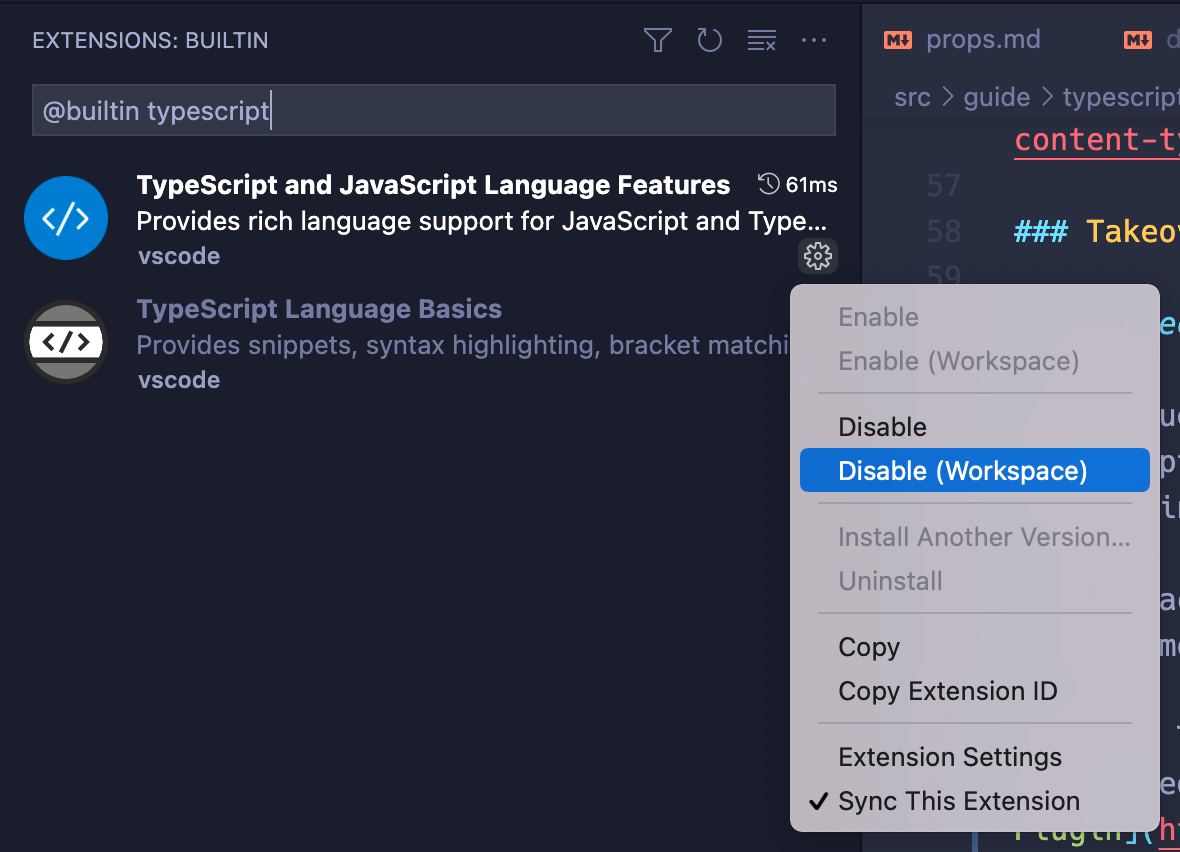
\includegraphics{./img/takeover-mode.54f7bbf6.png} 
\end{center}


\columnratio{0.55}
\begin{paracol}{2} 
 
\switchcolumn[0]*%%%%%%%
\subsubsection{Note on Vue CLI and ts-loader}
\switchcolumn
\subsubsection{关于 Vue CLI 和 ts-loader}
\switchcolumn[0]*%%%%%%%
In webpack-based setups such as Vue CLI, it is common to perform type
checking as part of the module transform pipeline, for example with
\texttt{ts-loader}. This, however, isn't a clean solution because the
type system needs knowledge of the entire module graph to perform type
checks. Individual module's transform step simply is not the right place
for the task. It leads to the following problems:
\switchcolumn
像 Vue CLI 这样的基于 webpack
搭建的项目,通常是在模块编译的过程中顺道执行类型检查,例如使用
\texttt{ts-loader}。然而这并不是一个理想的解决方案,因为类型系统需要了解整个模块关系才能执行类型检查。loader
中只适合单个模块的编译,并不适合做需要全局信息的工作。这导致了下面的问题:
\switchcolumn[0]*%%%%%%%
\begin{itemize}
\item
  \texttt{ts-loader} can only type check post-transform code. This
  doesn't align with the errors we see in IDEs or from \texttt{vue-tsc},
  which map directly back to the source code.
\item
  Type checking can be slow. When it is performed in the same thread /
  process with code transformations, it significantly affects the build
  speed of the entire application.
\item
  We already have type checking running right in our IDE in a separate
  process, so the cost of dev experience slow down simply isn't a good
  trade-off.
\end{itemize}
\switchcolumn
\begin{itemize}
\item
  \texttt{ts-loader} 只能对在它之前的 loader
  编译转换后的代码执行类型检查,这和我们在 IDE 或 \texttt{vue-tsc}
  中看到的基于源代码的错误提示并不一致。
\item
  类型检查可能会很慢。当它和代码转换在相同的线程/进程中执行时,它会显著影响整个应用的构建速度。
\item
  我们已经在 IDE
  中通过单独的进程运行着类型检查了,却还要在构建流程中执行类型检查导致降低开发体验,这似乎不太划算。
\end{itemize}
\switchcolumn[0]*%%%%%%%
If you are currently using Vue 3 + TypeScript via Vue CLI, we strongly
recommend migrating over to Vite. We are also working on CLI options to
enable transpile-only TS support, so that you can switch to
\texttt{vue-tsc} for type checking.
\switchcolumn
如果你正通过 Vue CLI 使用 Vue 3 和 TypeScript,我们强烈建议你迁移到
Vite。我们也在为 CLI 开发仅执行 TS 语法转译的选项,以允许你切换至
\texttt{vue-tsc} 来执行类型检查。
\end{paracol}



\columnratio{0.55}
\begin{paracol}{2} 
 
\switchcolumn[0]*%%%%%%%
\subsection{General Usage Notes}
\switchcolumn
\subsection{常见使用说明}
\switchcolumn[0]*%%%%%%%
\subsubsection{defineComponent()}
\switchcolumn
\subsubsection{defineComponent()}
\switchcolumn[0]*%%%%%%%
To let TypeScript properly infer types inside component options, we need
to define components with
\href{https://vuejs.org/api/general.html\#definecomponent}{\texttt{defineComponent()}}:
\switchcolumn
为了让 TypeScript 正确地推导出组件选项内的类型,我们需要通过
\href{https://cn.vuejs.org/api/general.html\#definecomponent}{\texttt{defineComponent()}}
这个全局 API 来定义组件:
\switchcolumn[0]*%%%%%%%
\begin{codeJs}
import { defineComponent } from 'vue'
export default defineComponent({
  // 启用了类型推导
  props: {
    name: String,
    msg: { type: String, required: true }
  },
  data() {
    return {
      count: 1
    }
  },
  mounted() {
    this.name // 类型:string | undefined
    this.msg // 类型:string
    this.count // 类型:number
  }
})
\end{codeJs}
\switchcolumn
\begin{codeJs}
import { defineComponent } from 'vue'
export default defineComponent({
  // 启用了类型推导
  props: {
    name: String,
    msg: { type: String, required: true }
  },
  data() {
    return {
      count: 1
    }
  },
  mounted() {
    this.name // 类型:string | undefined
    this.msg // 类型:string
    this.count // 类型:number
  }
})
\end{codeJs}
\switchcolumn[0]*%%%%%%%
\texttt{defineComponent()} also supports inferring the props passed to
\texttt{setup()} when using Composition API without
\texttt{\textless{}script\ setup\textgreater{}}:
\switchcolumn
当没有结合 \texttt{\textless{}script\ setup\textgreater{}} 使用组合式
API 时,\texttt{defineComponent()} 也支持对传递给 \texttt{setup()} 的
prop 的推导:
\switchcolumn[0]*%%%%%%%
\begin{codeJs}
import { defineComponent } from 'vue'
export default defineComponent({
  // 启用了类型推导
  props: {
    message: String
  },
  setup(props) {
    props.message // 类型:string | undefined
  }
})
\end{codeJs}
\switchcolumn
\begin{codeJs}
import { defineComponent } from 'vue'
export default defineComponent({
  // 启用了类型推导
  props: {
    message: String
  },
  setup(props) {
    props.message // 类型:string | undefined
  }
})
\end{codeJs}
\switchcolumn[0]*%%%%%%%
See also:
\switchcolumn
参考:
\switchcolumn[0]*%%%%%%%
\begin{itemize}
\item
  \href{https://vuejs.org/api/general.html\#note-on-webpack-treeshaking}{Note
  on webpack Treeshaking}
\item
  \href{https://github.com/vuejs/core/blob/main/packages/dts-test/defineComponent.test-d.tsx}{type
  tests for \texttt{defineComponent}}
\end{itemize}
\switchcolumn
\begin{itemize}
\item
  \href{https://cn.vuejs.org/api/general.html\#note-on-webpack-treeshaking}{webpack
  Treeshaking 的注意事项}
\item
  \href{https://github.com/vuejs/core/blob/main/packages/dts-test/defineComponent.test-d.tsx}{对
  \texttt{defineComponent} 的类型测试}
\end{itemize}
\switchcolumn[0]*%%%%%%%
\begin{vueQuote}{TIP}
\texttt{defineComponent()} also enables type inference for components
defined in plain JavaScript.
\end{vueQuote} 
\switchcolumn
\begin{vueQuote}{TIP}
\texttt{defineComponent()} 也支持对纯 JavaScript
编写的组件进行类型推导。
\end{vueQuote} 
\switchcolumn[0]*%%%%%%%
\subsubsection{Usage in Single-File Components}
\switchcolumn
\subsubsection{在单文件组件中的用法}
\switchcolumn[0]*%%%%%%%
To use TypeScript in SFCs, add the \texttt{lang="ts"} attribute to
\texttt{\textless{}script\textgreater{}} tags. When \texttt{lang="ts"}
is present, all template expressions also enjoy stricter type checking.
\switchcolumn
要在单文件组件中使用 TypeScript,需要在
\texttt{\textless{}script\textgreater{}} 标签上加上 \texttt{lang="ts"}
的 attribute。当 \texttt{lang="ts"}
存在时,所有的模板内表达式都将享受到更严格的类型检查。
\switchcolumn[0]*%%%%%%%
\begin{codeHtml}
<script lang="ts">
import { defineComponent } from 'vue'
export default defineComponent({
  data() {
    return {
      count: 1
    }
  }
})
</script>
<template>
  <!-- 启用了类型检查和自动补全 -->
  {{ count.toFixed(2) }}
</template>
\end{codeHtml}
\switchcolumn
\begin{codeHtml}
<script lang="ts">
import { defineComponent } from 'vue'
export default defineComponent({
  data() {
    return {
      count: 1
    }
  }
})
</script>
<template>
  <!-- 启用了类型检查和自动补全 -->
  {{ count.toFixed(2) }}
</template>
\end{codeHtml}
\switchcolumn[0]*%%%%%%%
\texttt{lang="ts"} can also be used with
\texttt{\textless{}script\ setup\textgreater{}}:
\switchcolumn
\texttt{lang="ts"} 也可以用于
\texttt{\textless{}script\ setup\textgreater{}}:
\switchcolumn[0]*%%%%%%%
\begin{codeHtml}
<script setup lang="ts">
// 启用了 TypeScript
import { ref } from 'vue'
const count = ref(1)
</script>
<template>
  <!-- 启用了类型检查和自动补全 -->
  {{ count.toFixed(2) }}
</template>
\end{codeHtml}
\switchcolumn
\begin{codeHtml}
<script setup lang="ts">
// 启用了 TypeScript
import { ref } from 'vue'
const count = ref(1)
</script>
<template>
  <!-- 启用了类型检查和自动补全 -->
  {{ count.toFixed(2) }}
</template>
\end{codeHtml}
\end{paracol}


\columnratio{0.55}
\begin{paracol}{2} 
 
\switchcolumn[0]*%%%%%%%
\subsubsection{TypeScript in Templates}
\switchcolumn
\subsubsection{模板中的 TypeScript}
\switchcolumn[0]*%%%%%%%
The \texttt{\textless{}template\textgreater{}} also supports TypeScript
in binding expressions when
\texttt{\textless{}script\ lang="ts"\textgreater{}} or
\texttt{\textless{}script\ setup\ lang="ts"\textgreater{}} is used. This
is useful in cases where you need to perform type casting in template
expressions.
\switchcolumn
在使用了 \texttt{\textless{}script\ lang="ts"\textgreater{}} 或
\texttt{\textless{}script\ setup\ lang="ts"\textgreater{}}
后,\texttt{\textless{}template\textgreater{}} 在绑定表达式中也支持
TypeScript。这对需要在模板表达式中执行类型转换的情况下非常有用。
\switchcolumn[0]*%%%%%%%
Here's a contrived example:
\switchcolumn
这里有一个假想的例子:
\switchcolumn[0]*%%%%%%%
\begin{codeHtml}
<script setup lang="ts">
let x: string | number = 1
</script>
<template>
  <!-- 出错,因为 x 可能是字符串 -->
  {{ x.toFixed(2) }}
</template>
\end{codeHtml}
\switchcolumn
\begin{codeHtml}
<script setup lang="ts">
let x: string | number = 1
</script>
<template>
  <!-- 出错,因为 x 可能是字符串 -->
  {{ x.toFixed(2) }}
</template>
\end{codeHtml}
\switchcolumn[0]*%%%%%%%
This can be worked around with an inline type cast:
\switchcolumn
可以使用内联类型强制转换解决此问题:
\switchcolumn[0]*%%%%%%%
\begin{codeHtml}
<script setup lang="ts">
let x: string | number = 1
</script>
<template>
  {{ (x as number).toFixed(2) }}
</template>
\end{codeHtml}
\switchcolumn
\begin{codeHtml}
<script setup lang="ts">
let x: string | number = 1
</script>
<template>
  {{ (x as number).toFixed(2) }}
</template>
\end{codeHtml}
\switchcolumn[0]*%%%%%%%
\begin{vueQuote}{TIP}
If using Vue CLI or a webpack-based setup, TypeScript in template
expressions requires \texttt{vue-loader@\^{}16.8.0}.
\end{vueQuote} 
\switchcolumn
\begin{vueQuote}{TIP}
如果正在使用 Vue CLI 或基于 webpack 的配置,支持模板内表达式的
TypeScript 需要 \texttt{vue-loader@\^{}16.8.0}。
\end{vueQuote} 
\end{paracol}



\columnratio{0.55}
\begin{paracol}{2} 
 
\switchcolumn[0]*%%%%%%%
\subsubsection{Usage with TSX}
\switchcolumn
\subsubsection{使用 TSX}
\switchcolumn[0]*%%%%%%%
Vue also supports authoring components with JSX / TSX. Details are
covered in the
\href{https://vuejs.org/guide/extras/render-function.html\#jsx-tsx}{Render
Function \& JSX} guide.
\switchcolumn
Vue 也支持使用 JSX / TSX
编写组件。详情请查阅\href{https://cn.vuejs.org/guide/extras/render-function.html\#jsx-tsx}{渲染函数
\& JSX}。
\switchcolumn[0]*%%%%%%%
\subsection{Generic Components}
\switchcolumn
\subsection{泛型组件}
\switchcolumn[0]*%%%%%%%
Generic components are supported in two cases:
\switchcolumn
泛型组件支持两种使用方式:
\switchcolumn[0]*%%%%%%%
\begin{itemize}
\item
  In SFCs:
  \href{https://vuejs.org/api/sfc-script-setup.html\#generics}{\texttt{\textasciigrave{}\ with\ the}generic`
  attribute}
\item
  Render function / JSX components:
  \href{https://vuejs.org/api/general.html\#function-signature}{\texttt{defineComponent()}'s
  function signature}
\end{itemize}
\switchcolumn
\begin{itemize}
\item
  在单文件组件中:\href{https://cn.vuejs.org/api/sfc-script-setup.html\#generics}{在
  \texttt{\textasciigrave{}\ 上使用}generic` 属性}
\item
  渲染函数 / JSX
  组件:\href{https://cn.vuejs.org/api/general.html\#function-signature}{\texttt{defineComponent()}
  的函数签名}
\end{itemize}
\switchcolumn[0]*%%%%%%%
\subsection{API-Specific Recipes}
\switchcolumn
\subsection{特定 API 的使用指南}
\switchcolumn[0]*%%%%%%%
\begin{itemize}
\item
  \href{https://vuejs.org/guide/typescript/composition-api.html}{TS with
  Composition API}
\item
  \href{https://vuejs.org/guide/typescript/options-api.html}{TS with
  Options API}
\end{itemize}
\switchcolumn
\begin{itemize}
\item
  \href{https://cn.vuejs.org/guide/typescript/composition-api.html}{TS
  与组合式 API}
\item
  \href{https://cn.vuejs.org/guide/typescript/options-api.html}{TS
  与选项式 API}
\end{itemize}
\end{paracol}

 %todo 看
\columnratio{0.55}
\begin{paracol}{2} 
 
\switchcolumn[0]*%%%%%%%
\section{TypeScript with Composition API}
\switchcolumn
\section{TypeScript 与组合式 API}
\switchcolumn[0]*%%%%%%%
\begin{quote}
This page assumes you've already read the overview on
\href{https://vuejs.org/guide/typescript/overview.html}{Using Vue with
TypeScript}.
\end{quote}
\switchcolumn
\begin{quote}
这一章假设你已经阅读了\href{https://cn.vuejs.org/guide/typescript/overview.html}{搭配
TypeScript 使用 Vue} 的概览。
\end{quote}
\end{paracol}


\columnratio{0.55}
\begin{paracol}{2} 
 
\switchcolumn[0]*%%%%%%%
\subsection{Typing Component Props}
\switchcolumn
\subsection{为组件的 props 标注类型}
\switchcolumn[0]*%%%%%%%
\subsubsection{Using \textless script setup\textgreater{}}
\switchcolumn
\subsubsection{使用 \textless script setup\textgreater{}}
\switchcolumn[0]*%%%%%%%
When using \texttt{\textless{}script\ setup\textgreater{}}, the
\texttt{defineProps()} macro supports inferring the props types based on
its argument:
\switchcolumn
当使用 \texttt{\textless{}script\ setup\textgreater{}}
时,\texttt{defineProps()} 宏函数支持从它的参数中推导类型:
\switchcolumn[0]*%%%%%%%
\begin{codeHtml}
<script setup lang="ts">
const props = defineProps({
  foo: { type: String, required: true },
  bar: Number
})
props.foo // string
props.bar // number | undefined
</script>
\end{codeHtml}
\switchcolumn
\begin{codeHtml}
<script setup lang="ts">
const props = defineProps({
  foo: { type: String, required: true },
  bar: Number
})
props.foo // string
props.bar // number | undefined
</script>
\end{codeHtml}
\switchcolumn[0]*%%%%%%%
This is called "runtime declaration", because the argument passed to
\texttt{defineProps()} will be used as the runtime \texttt{props}
option.
\switchcolumn
这被称之为``运行时声明'',因为传递给 \texttt{defineProps()}
的参数会作为运行时的 \texttt{props} 选项使用。
\switchcolumn[0]*%%%%%%%
However, it is usually more straightforward to define props with pure
types via a generic type argument:
\switchcolumn
然而,通过泛型参数来定义 props 的类型通常更直接:
\switchcolumn[0]*%%%%%%%
\begin{codeHtml}
<script setup lang="ts">
const props = defineProps<{
  foo: string
  bar?: number
}>()
</script>
\end{codeHtml}
\switchcolumn
\begin{codeHtml}
<script setup lang="ts">
const props = defineProps<{
  foo: string
  bar?: number
}>()
</script>
\end{codeHtml}
\switchcolumn[0]*%%%%%%%
This is called "type-based declaration". The compiler will try to do its
best to infer the equivalent runtime options based on the type argument.
In this case, our second example compiles into the exact same runtime
options as the first example.
\switchcolumn
这被称之为``基于类型的声明''。编译器会尽可能地尝试根据类型参数推导出等价的运行时选项。在这种场景下,我们第二个例子中编译出的运行时选项和第一个是完全一致的。
\switchcolumn[0]*%%%%%%%
You can use either type-based declaration OR runtime declaration, but
you cannot use both at the same time.
\switchcolumn
基于类型的声明或者运行时声明可以择一使用,但是不能同时使用。
\switchcolumn[0]*%%%%%%%
We can also move the props types into a separate interface:
\switchcolumn
我们也可以将 props 的类型移入一个单独的接口中:
\switchcolumn[0]*%%%%%%%
\begin{codeHtml}
<script setup lang="ts">
interface Props {
  foo: string
  bar?: number
}
const props = defineProps<Props>()
</script>
\end{codeHtml}
\switchcolumn
\begin{codeHtml}
<script setup lang="ts">
interface Props {
  foo: string
  bar?: number
}
const props = defineProps<Props>()
</script>
\end{codeHtml}
\switchcolumn[0]*%%%%%%%
\paragraph{Syntax Limitations}
\switchcolumn
\paragraph{语法限制}
\switchcolumn[0]*%%%%%%%
In version 3.2 and below, the generic type parameter for
\texttt{defineProps()} were limited to a type literal or a reference to
a local interface.
\switchcolumn
在 3.2 及以下版本中,\texttt{defineProps()}
的泛型类型参数仅限于类型文字或对本地接口的引用。
\end{paracol}



\columnratio{0.55}
\begin{paracol}{2} 
 
\switchcolumn[0]*%%%%%%%
This limitation has been resolved in 3.3. The latest version of Vue
supports referencing imported and a limited set of complex types in the
type parameter position. However, because the type to runtime conversion
is still AST-based, some complex types that require actual type
analysis, e.g. conditional types, are not supported. You can use
conditional types for the type of a single prop, but not the entire
props object.
\switchcolumn
这个限制在 3.3 中得到了解决。最新版本的 Vue
支持在类型参数位置引用导入和有限的复杂类型。但是,由于类型到运行时转换仍然基于
AST,一些需要实际类型分析的复杂类型,例如条件类型,还未支持。您可以使用条件类型来指定单个
prop 的类型,但不能用于整个 props 对象的类型。
\switchcolumn[0]*%%%%%%%
\subsubsection{Props Default Values}
\switchcolumn
\subsubsection{Props 解构默认值}
\switchcolumn[0]*%%%%%%%
When using type-based declaration, we lose the ability to declare
default values for the props. This can be resolved by the
\texttt{withDefaults} compiler macro:
\begin{codeTs}
export interface Props {
  msg?: string
  labels?: string[]
}
const props = withDefaults(defineProps<Props>(), {
  msg: 'hello',
  labels: () => ['one', 'two'] 
})
\end{codeTs}
\switchcolumn
当使用基于类型的声明时,我们失去了为 props 声明默认值的能力。这可以通过
\texttt{withDefaults} 编译器宏解决:
\begin{codeTs}
    export interface Props {
      msg?: string
      labels?: string[]
    }
    const props = withDefaults(defineProps<Props>(), {
      msg: 'hello',
      labels: () => ['one', 'two']
    })
    \end{codeTs}
\end{paracol}



\columnratio{0.55}
\begin{paracol}{2} 

\end{paracol}


\columnratio{0.55}
\begin{paracol}{2} 

\end{paracol}



\columnratio{0.55}
\begin{paracol}{2} 

\end{paracol}%todo 看
\columnratio{0.55}
\begin{paracol}{2} 
 
\switchcolumn[0]*%%%%%%%
\section{TypeScript with Composition API}
\switchcolumn
\section{TypeScript 与选项式 API}
\switchcolumn[0]*%%%%%%%
\begin{quote}
This page assumes you've already read the overview on
\href{https://vuejs.org/guide/typescript/overview.html}{Using Vue with
TypeScript}.
\end{quote}
\switchcolumn
\begin{quote}
这一章假设你已经阅读了\href{https://cn.vuejs.org/guide/typescript/overview.html}{搭配
TypeScript 使用 Vue} 的概览。
\end{quote}
\switchcolumn[0]*%%%%%%%
\begin{vueQuote}{TIP}
While Vue does support TypeScript usage with Options API, it is recommended to use Vue with TypeScript via Composition API as it offers simpler, more efficient and more robust type inference.
\end{vueQuote} 
\switchcolumn
\begin{vueQuote}{TIP}
虽然 Vue 的确支持在选项式 API 中使用 TypeScript,但在使用 TypeScript
的前提下更推荐使用组合式 API,因为它提供了更简单、高效和可靠的类型推导。
\end{vueQuote} 
\switchcolumn[0]*%%%%%%%
\subsection{Typing Component Props}
\switchcolumn
\subsection{为组件的 props 标注类型}
\switchcolumn[0]*%%%%%%%
Type inference for props in Options API requires wrapping the component
with \texttt{defineComponent()}. With it, Vue is able to infer the types
for the props based on the \texttt{props} option, taking additional
options such as \texttt{required:\ true} and \texttt{default} into
account:
\switchcolumn
选项式 API 中对 props 的类型推导需要用 \texttt{defineComponent()}
来包装组件。有了它,Vue 才可以通过 \texttt{props}
以及一些额外的选项,比如 \texttt{required:\ true} 和 \texttt{default}
来推导出 props 的类型:
\switchcolumn[0]*%%%%%%%
\begin{codeTs}
import { defineComponent } from 'vue'
export default defineComponent({
  // 启用了类型推导
  props: {
    name: String,
    id: [Number, String],
    msg: { type: String, required: true },
    metadata: null
  },
  mounted() {
    this.name // 类型:string | undefined
    this.id // 类型:number | string | undefined
    this.msg // 类型:string
    this.metadata // 类型:any
  }
})
\end{codeTs}
\switchcolumn
\begin{codeTs}
import { defineComponent } from 'vue'
export default defineComponent({
    // 启用了类型推导
    props: {
    name: String,
    id: [Number, String],
    msg: { type: String, required: true },
    metadata: null
    },
    mounted() {
    this.name // 类型:string | undefined
    this.id // 类型:number | string | undefined
    this.msg // 类型:string
    this.metadata // 类型:any
    }
})
\end{codeTs}
\switchcolumn[0]*%%%%%%%
However, the runtime \texttt{props} options only support using
constructor functions as a prop's type - there is no way to specify
complex types such as objects with nested properties or function call
signatures.
\switchcolumn
然而,这种运行时 \texttt{props} 选项仅支持使用构造函数来作为一个 prop
的类型------没有办法指定多层级对象或函数签名之类的复杂类型。
\switchcolumn[0]*%%%%%%%
To annotate complex props types, we can use the \texttt{PropType}
utility type:
\switchcolumn
我们可以使用 \texttt{PropType} 这个工具类型来标记更复杂的 props 类型:
\switchcolumn[0]*%%%%%%%
\begin{codeTs}
import { defineComponent } from 'vue'
import type { PropType } from 'vue'
interface Book {
  title: string
  author: string
  year: number
}
export default defineComponent({
  props: {
    book: {
      // 提供相对 `Object` 更确定的类型
      type: Object as PropType<Book>,
      required: true
    },
    // 也可以标记函数
    callback: Function as PropType<(id: number) => void>
  },
  mounted() {
    this.book.title // string
    this.book.year // number
    // TS Error: argument of type 'string' is not
    // assignable to parameter of type 'number'
    this.callback?.('123')
  }
})
\end{codeTs}
\switchcolumn
\begin{codeTs}
import { defineComponent } from 'vue'
import type { PropType } from 'vue'
interface Book {
  title: string
  author: string
  year: number
}
export default defineComponent({
  props: {
    book: {
      // 提供相对 `Object` 更确定的类型
      type: Object as PropType<Book>,
      required: true
    },
    // 也可以标记函数
    callback: Function as PropType<(id: number) => void>
  },
  mounted() {
    this.book.title // string
    this.book.year // number
    // TS Error: argument of type 'string' is not
    // assignable to parameter of type 'number'
    this.callback?.('123')
  }
})
\end{codeTs}
\switchcolumn[0]*%%%%%%%
\subsubsection{Caveats}
\switchcolumn
\subsubsection{注意事项}
\switchcolumn[0]*%%%%%%%
If your TypeScript version is less than \texttt{4.7}, you have to be
careful when using function values for \texttt{validator} and
\texttt{default} prop options - make sure to use arrow functions:
\switchcolumn
如果你的 TypeScript 版本低于 \texttt{4.7},在使用函数作为 prop 的
\texttt{validator} 和 \texttt{default}
选项值时需要格外小心------确保使用箭头函数:
\switchcolumn[0]*%%%%%%%
\begin{codeTs}
import { defineComponent } from 'vue'
import type { PropType } from 'vue'
interface Book {
  title: string
  year?: number
}
export default defineComponent({
  props: {
    bookA: {
      type: Object as PropType<Book>,
      // 如果你的 TypeScript 版本低于 4.7,确保使用箭头函数
      default: () => ({
        title: 'Arrow Function Expression'
      }),
      validator: (book: Book) => !!book.title
    }
  }
})
\end{codeTs}
\switchcolumn
\begin{codeTs}
import { defineComponent } from 'vue'
import type { PropType } from 'vue'
interface Book {
  title: string
  year?: number
}
export default defineComponent({
  props: {
    bookA: {
      type: Object as PropType<Book>,
      // 如果你的 TypeScript 版本低于 4.7,确保使用箭头函数
      default: () => ({
        title: 'Arrow Function Expression'
      }),
      validator: (book: Book) => !!book.title
    }
  }
})
\end{codeTs}
\switchcolumn[0]*%%%%%%%
This prevents TypeScript from having to infer the type of \texttt{this}
inside these functions, which, unfortunately, can cause the type
inference to fail. It was a previous
\href{https://github.com/microsoft/TypeScript/issues/38845}{design
limitation}, and now has been improved in
\href{https://www.typescriptlang.org/docs/handbook/release-notes/typescript-4-7.html\#improved-function-inference-in-objects-and-methods}{TypeScript
4.7}.
\switchcolumn
这会防止 TypeScript 将 \texttt{this}
根据函数内的环境作出不符合我们期望的类型推导。这是之前版本的一个\href{https://github.com/microsoft/TypeScript/issues/38845}{设计限制},不过现在已经在
\href{https://www.typescriptlang.org/docs/handbook/release-notes/typescript-4-7.html\#improved-function-inference-in-objects-and-methods}{TypeScript
4.7} 中解决了。
\switchcolumn[0]*%%%%%%%
\subsection{Typing Component Emits}
\switchcolumn
\subsection{为组件的 emits 标注类型}
\switchcolumn[0]*%%%%%%%
We can declare the expected payload type for an emitted event using the
object syntax of the \texttt{emits} option. Also, all non-declared
emitted events will throw a type error when called:
\switchcolumn
我们可以给 \texttt{emits}
选项提供一个对象来声明组件所触发的事件,以及这些事件所期望的参数类型。试图触发未声明的事件会抛出一个类型错误:
\switchcolumn[0]*%%%%%%%
\begin{codeTs}
import { defineComponent } from 'vue'
export default defineComponent({
  emits: {
    addBook(payload: { bookName: string }) {
      // 执行运行时校验
      return payload.bookName.length > 0
    }
  },
  methods: {
    onSubmit() {
      this.$emit('addBook', {
        bookName: 123 // 类型错误
      })
      this.$emit('non-declared-event') // 类型错误
    }
  }
})
\end{codeTs}
\switchcolumn
\begin{codeTs}
import { defineComponent } from 'vue'
export default defineComponent({
  emits: {
    addBook(payload: { bookName: string }) {
      // 执行运行时校验
      return payload.bookName.length > 0
    }
  },
  methods: {
    onSubmit() {
      this.$emit('addBook', {
        bookName: 123 // 类型错误
      })
      this.$emit('non-declared-event') // 类型错误
    }
  }
})
\end{codeTs}
\end{paracol}


\columnratio{0.55}
\begin{paracol}{2} 
 
\switchcolumn[0]*%%%%%%%
\subsection{Typing Computed Properties}
\switchcolumn
\subsection{为计算属性标记类型}
\switchcolumn[0]*%%%%%%%
A computed property infers its type based on its return value:
\switchcolumn
计算属性会自动根据其返回值来推导其类型:
\switchcolumn[0]*%%%%%%%
\begin{codeTs}
import { defineComponent } from 'vue'
export default defineComponent({
  data() {
    return {
      message: 'Hello!'
    }
  },
  computed: {
    greeting() {
      return this.message + '!'
    }
  },
  mounted() {
    this.greeting // 类型:string
  }
})
\end{codeTs}
\switchcolumn
\begin{codeTs}
import { defineComponent } from 'vue'
export default defineComponent({
  data() {
    return {
      message: 'Hello!'
    }
  },
  computed: {
    greeting() {
      return this.message + '!'
    }
  },
  mounted() {
    this.greeting // 类型:string
  }
})
\end{codeTs}
\switchcolumn[0]*%%%%%%%
In some cases, you may want to explicitly annotate the type of a
computed property to ensure its implementation is correct:
\switchcolumn
在某些场景中,你可能想要显式地标记出计算属性的类型以确保其实现是正确的:
\switchcolumn[0]*%%%%%%%
\begin{codeTs}
import { defineComponent } from 'vue'
export default defineComponent({
  data() {
    return {
      message: 'Hello!'
    }
  },
  computed: {
    // 显式标注返回类型
    greeting(): string {
      return this.message + '!'
    },
    // 标注一个可写的计算属性
    greetingUppercased: {
      get(): string {
        return this.greeting.toUpperCase()
      },
      set(newValue: string) {
        this.message = newValue.toUpperCase()
      }
    }
  }
})
\end{codeTs}
\switchcolumn
\begin{codeTs}
import { defineComponent } from 'vue'
export default defineComponent({
  data() {
    return {
      message: 'Hello!'
    }
  },
  computed: {
    // 显式标注返回类型
    greeting(): string {
      return this.message + '!'
    },
    // 标注一个可写的计算属性
    greetingUppercased: {
      get(): string {
        return this.greeting.toUpperCase()
      },
      set(newValue: string) {
        this.message = newValue.toUpperCase()
      }
    }
  }
})
\end{codeTs}
\switchcolumn[0]*%%%%%%%
Explicit annotations may also be required in some edge cases where
TypeScript fails to infer the type of a computed property due to
circular inference loops.
\switchcolumn
在某些 TypeScript
因循环引用而无法推导类型的情况下,可能必须进行显式的类型标注。
\end{paracol}

\columnratio{0.55}
\begin{paracol}{2} 
 
\switchcolumn[0]*%%%%%%%
\subsection{Typing Event Handlers}
\switchcolumn
\subsection{为事件处理函数标注类型}
\switchcolumn[0]*%%%%%%%
When dealing with native DOM events, it might be useful to type the
argument we pass to the handler correctly. Let's take a look at this
example:
\switchcolumn
在处理原生 DOM
事件时,应该为我们传递给事件处理函数的参数正确地标注类型。让我们看一下这个例子:
\switchcolumn[0]*%%%%%%%
\begin{codeHtml}
<script lang="ts">
import { defineComponent } from 'vue'
export default defineComponent({
  methods: {
    handleChange(event) {
      // `event` 隐式地标注为 `any` 类型
      console.log(event.target.value)
    }
  }
})
</script>
<template>
  <input type="text" @change="handleChange" />
</template>
\end{codeHtml}
\switchcolumn
\begin{codeHtml}
<script lang="ts">
import { defineComponent } from 'vue'
export default defineComponent({
  methods: {
    handleChange(event) {
      // `event` 隐式地标注为 `any` 类型
      console.log(event.target.value)
    }
  }
})
</script>
<template>
  <input type="text" @change="handleChange" />
</template>
\end{codeHtml}
\switchcolumn[0]*%%%%%%%
Without type annotation, the \texttt{event} argument will implicitly
have a type of \texttt{any}. This will also result in a TS error if
\texttt{"strict":\ true} or \texttt{"noImplicitAny":\ true} are used in
\texttt{tsconfig.json}. It is therefore recommended to explicitly
annotate the argument of event handlers. In addition, you may need to
use type assertions when accessing the properties of \texttt{event}:
\switchcolumn
没有类型标注时,这个 \texttt{event} 参数会隐式地标注为 \texttt{any}
类型。这也会在 \texttt{tsconfig.json} 中配置了 \texttt{"strict":\ true}
或 \texttt{"noImplicitAny":\ true} 时抛出一个 TS
错误。因此,建议显式地为事件处理函数的参数标注类型。此外,在访问
\texttt{event} 上的属性时你可能需要使用类型断言:
\switchcolumn[0]*%%%%%%%
\begin{codeTs}
import { defineComponent } from 'vue'
export default defineComponent({
  methods: {
    handleChange(event: Event) {
      console.log((event.target as HTMLInputElement).value)
    }
  }
})
\end{codeTs}
\switchcolumn
\begin{codeTs}
import { defineComponent } from 'vue'
export default defineComponent({
  methods: {
    handleChange(event: Event) {
      console.log((event.target as HTMLInputElement).value)
    }
  }
})
\end{codeTs}
\end{paracol}


\columnratio{0.55}
\begin{paracol}{2} 
 
\switchcolumn[0]*%%%%%%%
\subsection{Augmenting Global Properties}
\switchcolumn
\subsection{扩展全局属性}
\switchcolumn[0]*%%%%%%%
Some plugins install globally available properties to all component
instances via
\href{https://vuejs.org/api/application.html\#app-config-globalproperties}{\texttt{app.config.globalProperties}}.
For example, we may install \texttt{this.\$http} for data-fetching or
\texttt{this.\$translate} for internationalization. To make this play
well with TypeScript, Vue exposes a \texttt{ComponentCustomProperties}
interface designed to be augmented via
\href{https://www.typescriptlang.org/docs/handbook/declaration-merging.html\#module-augmentation}{TypeScript
module augmentation}:
\switchcolumn
某些插件会通过
\href{https://cn.vuejs.org/api/application.html\#app-config-globalproperties}{\texttt{app.config.globalProperties}}
为所有组件都安装全局可用的属性。举例来说,我们可能为了请求数据而安装了
\texttt{this.\$http},或者为了国际化而安装了
\texttt{this.\$translate}。为了使 TypeScript 更好地支持这个行为,Vue
暴露了一个被设计为可以通过
\href{https://www.typescriptlang.org/docs/handbook/declaration-merging.html\#module-augmentation}{TypeScript
模块扩展}来扩展的 \texttt{ComponentCustomProperties} 接口:
\switchcolumn[0]*%%%%%%%
\begin{codeTs}
import axios from 'axios'
declare module 'vue' {
  interface ComponentCustomProperties {
    $http: typeof axios
    $translate: (key: string) => string
  }
}
\end{codeTs}
\switchcolumn
\begin{codeTs}
import axios from 'axios'
declare module 'vue' {
  interface ComponentCustomProperties {
    $http: typeof axios
    $translate: (key: string) => string
  }
}
\end{codeTs}
\switchcolumn[0]*%%%%%%%
See also:
\switchcolumn
参考:
\switchcolumn[0]*%%%%%%%
\begin{itemize}
\item
  \href{https://github.com/vuejs/core/blob/main/packages/dts-test/componentTypeExtensions.test-d.tsx}{TypeScript
  unit tests for component type extensions}
\end{itemize}
\switchcolumn
\begin{itemize}
\item
  \href{https://github.com/vuejs/core/blob/main/packages/dts-test/componentTypeExtensions.test-d.tsx}{对组件类型扩展的
  TypeScript 单元测试}
\end{itemize}
\switchcolumn[0]*%%%%%%%
\subsubsection{Type Augmentation Placement}
\switchcolumn
\subsubsection{类型扩展的位置}
\switchcolumn[0]*%%%%%%%
We can put this type augmentation in a \texttt{.ts} file, or in a
project-wide \texttt{*.d.ts} file. Either way, make sure it is included
in \texttt{tsconfig.json}. For library / plugin authors, this file
should be specified in the \texttt{types} property in
\texttt{package.json}.
\switchcolumn
我们可以将这些类型扩展放在一个 \texttt{.ts} 文件,或是一个影响整个项目的
\texttt{*.d.ts} 文件中。无论哪一种,都应确保在 \texttt{tsconfig.json}
中包括了此文件。对于库或插件作者,这个文件应该在 \texttt{package.json}
的 \texttt{types} 属性中被列出。
\switchcolumn[0]*%%%%%%%
In order to take advantage of module augmentation, you will need to
ensure the augmentation is placed in a
\href{https://www.typescriptlang.org/docs/handbook/modules.html}{TypeScript
module}. That is to say, the file needs to contain at least one
top-level \texttt{import} or \texttt{export}, even if it is just
\texttt{export\ \{\}}. If the augmentation is placed outside of a
module, it will overwrite the original types rather than augmenting
them!
\switchcolumn
为了利用模块扩展的优势,你需要确保将扩展的模块放在
\href{https://www.typescriptlang.org/docs/handbook/modules.html}{TypeScript
模块} 中。 也就是说,该文件需要包含至少一个顶级的 \texttt{import} 或
\texttt{export},即使它只是
\texttt{export\ \{\}}。如果扩展被放在模块之外,它将覆盖原始类型,而不是扩展!
\switchcolumn[0]*%%%%%%%
\begin{codeTs}
// 不工作,将覆盖原始类型。
declare module 'vue' {
  interface ComponentCustomProperties {
    $translate: (key: string) => string
  }
}
\end{codeTs}
\switchcolumn
\begin{codeTs}
// 不工作,将覆盖原始类型。
declare module 'vue' {
  interface ComponentCustomProperties {
    $translate: (key: string) => string
  }
}
\end{codeTs}
\switchcolumn[0]*%%%%%%%
\begin{codeTs}
// 正常工作。
export {}
declare module 'vue' {
  interface ComponentCustomProperties {
    $translate: (key: string) => string
  }
}
\end{codeTs}
\switchcolumn
\begin{codeTs}
// 正常工作。
export {}
declare module 'vue' {
  interface ComponentCustomProperties {
    $translate: (key: string) => string
  }
}
\end{codeTs}
\switchcolumn[0]*%%%%%%%
\subsection{Augmenting Custom Options}
\switchcolumn
\subsection{扩展自定义选项}
\switchcolumn[0]*%%%%%%%
Some plugins, for example \texttt{vue-router}, provide support for
custom component options such as \texttt{beforeRouteEnter}:
\switchcolumn
某些插件,比如 \texttt{vue-router},提供了一些自定义的组件选项,比如
\texttt{beforeRouteEnter}:
\switchcolumn[0]*%%%%%%%
\begin{codeTs}
import { defineComponent } from 'vue'
export default defineComponent({
  beforeRouteEnter(to, from, next) {
    // ...
  }
})
\end{codeTs}
\switchcolumn
\begin{codeTs}
import { defineComponent } from 'vue'
export default defineComponent({
  beforeRouteEnter(to, from, next) {
    // ...
  }
})
\end{codeTs}
\switchcolumn[0]*%%%%%%%
Without proper type augmentation, the arguments of this hook will
implicitly have \texttt{any} type. We can augment the
\texttt{ComponentCustomOptions} interface to support these custom
options:
\switchcolumn
如果没有确切的类型标注,这个钩子函数的参数会隐式地标注为 \texttt{any}
类型。我们可以为 \texttt{ComponentCustomOptions}
接口扩展自定义的选项来支持:
\switchcolumn[0]*%%%%%%%
\begin{codeTs}
import { Route } from 'vue-router'
declare module 'vue' {
  interface ComponentCustomOptions {
    beforeRouteEnter?(to: Route, from: Route, next: () => void): void
  }
}
\end{codeTs}
\switchcolumn
\begin{codeTs}
import { Route } from 'vue-router'
declare module 'vue' {
  interface ComponentCustomOptions {
    beforeRouteEnter?(to: Route, from: Route, next: () => void): void
  }
}
\end{codeTs}
\switchcolumn[0]*%%%%%%%
Now the \texttt{beforeRouteEnter} option will be properly typed. Note
this is just an example - well-typed libraries like \texttt{vue-router}
should automatically perform these augmentations in their own type
definitions.
\switchcolumn
现在这个 \texttt{beforeRouteEnter}
选项会被准确地标注类型。注意这只是一个例子------像 \texttt{vue-router}
这种类型完备的库应该在它们自己的类型定义中自动执行这些扩展。
\switchcolumn[0]*%%%%%%%
The placement of this augmentation is subject the
\href{https://vuejs.org/guide/typescript/options-api.html\#type-augmentation-placement}{same
restrictions} as global property augmentations.
\switchcolumn
这种类型扩展和全局属性扩展受到\href{https://cn.vuejs.org/guide/typescript/options-api.html\#type-augmentation-placement}{相同的限制}。
\switchcolumn[0]*%%%%%%%
See also:
\switchcolumn
参考:
\switchcolumn[0]*%%%%%%%
\begin{itemize}
\item
  \href{https://github.com/vuejs/core/blob/main/packages/dts-test/componentTypeExtensions.test-d.tsx}{TypeScript
  unit tests for component type extensions}
\end{itemize}
\switchcolumn
\begin{itemize}
\item
  \href{https://github.com/vuejs/core/blob/main/packages/dts-test/componentTypeExtensions.test-d.tsx}{对组件类型扩展的
  TypeScript 单元测试}
\end{itemize}
\end{paracol}

\columnratio{0.55}
\begin{paracol}{2} 

\end{paracol}


\columnratio{0.55}
\begin{paracol}{2} 

\end{paracol}%todo 看
\chapter{Extra Topics\hfill }

\columnratio{0.55}
\begin{paracol}{2} 
 
\switchcolumn[0]*%%%%%%%
\section{Ways of Using Vue}
\switchcolumn
\section{使用 Vue 的多种方式}
\switchcolumn[0]*%%%%%%%
We believe there is no "one size fits all" story for the web. This is
why Vue is designed to be flexible and incrementally adoptable.
Depending on your use case, Vue can be used in different ways to strike
the optimal balance between stack complexity, developer experience and
end performance.
\switchcolumn
我们相信在 Web 的世界里没有一种方案可以解决所有问题。正因如此,Vue
被设计成一个灵活的、可以渐进式集成的框架。根据使用场景的不同需要,相应地有多种不同的方式来使用
Vue,以此在技术栈复杂度、开发体验和性能表现间取得最佳平衡。
\switchcolumn[0]*%%%%%%%
\subsection{Standalone Script}
\switchcolumn
\subsection{独立脚本}
\switchcolumn[0]*%%%%%%%
Vue can be used as a standalone script file - no build step required! If
you have a backend framework already rendering most of the HTML, or your
frontend logic isn't complex enough to justify a build step, this is the
easiest way to integrate Vue into your stack. You can think of Vue as a
more declarative replacement of jQuery in such cases.
\switchcolumn
Vue 可以以一个单独 JS
文件的形式使用,无需构建步骤!如果你的后端框架已经渲染了大部分的
HTML,或者你的前端逻辑并不复杂,不需要构建步骤,这是最简单的使用 Vue
的方式。在这些场景中你可以将 Vue 看作一个更加声明式的 jQuery 替代品。
\switchcolumn[0]*%%%%%%%
Vue also provides an alternative distribution called
\href{https://github.com/vuejs/petite-vue}{petite-vue} that is
specifically optimized for progressively enhancing existing HTML. It has
a smaller feature set, but is extremely lightweight and uses an
implementation that is more efficient in no-build-step scenarios.
\switchcolumn
Vue 也提供了另一个更适用于此类无构建步骤场景的版本
\href{https://github.com/vuejs/petite-vue}{petite-vue}。它为渐进式增强已有的
HTML 作了特别的优化,功能更加精简,十分轻量。
\switchcolumn[0]*%%%%%%%
\subsection{Embedded Web Components}
\switchcolumn
\subsection{作为 Web Component 嵌入}
\switchcolumn[0]*%%%%%%%
You can use Vue to
\href{https://vuejs.org/guide/extras/web-components.html}{build standard
Web Components} that can be embedded in any HTML page, regardless of how
they are rendered. This option allows you to leverage Vue in a
completely consumer-agnostic fashion: the resulting web components can
be embedded in legacy applications, static HTML, or even applications
built with other frameworks.
\switchcolumn
你可以用 Vue
来\href{https://cn.vuejs.org/guide/extras/web-components.html}{构建标准的
Web Component},这些 Web Component 可以嵌入到任何 HTML
页面中,无论它们是如何被渲染的。这个方式让你能够在不需要顾虑最终使用场景的情况下使用
Vue:因为生成的 Web Component 可以嵌入到旧应用、静态
HTML,甚至用其他框架构建的应用中。
\switchcolumn[0]*%%%%%%%
\subsection{Single-Page Application (SPA)}
\switchcolumn
\subsection{单页面应用 (SPA)}
\switchcolumn[0]*%%%%%%%
Some applications require rich interactivity, deep session depth, and
non-trivial stateful logic on the frontend. The best way to build such
applications is to use an architecture where Vue not only controls the
entire page, but also handles data updates and navigation without having
to reload the page. This type of application is typically referred to as
a Single-Page Application (SPA).
\switchcolumn
一些应用在前端需要具有丰富的交互性、较深的会话和复杂的状态逻辑。构建这类应用的最佳方法是使用这样一种架构:Vue
不仅控制整个页面,还负责处理抓取新数据,并在无需重新加载的前提下处理页面切换。这种类型的应用通常称为单页应用
(Single-Page application,缩写为 SPA)。
\switchcolumn[0]*%%%%%%%
Vue provides core libraries and
\href{https://vuejs.org/guide/scaling-up/tooling.html}{comprehensive
tooling support} with amazing developer experience for building modern
SPAs, including:
\switchcolumn
Vue
提供了核心功能库和\href{https://cn.vuejs.org/guide/scaling-up/tooling.html}{全面的工具链支持},为现代
SPA 提供了极佳的开发体验,覆盖以下方面:
\switchcolumn[0]*%%%%%%%
\begin{itemize}
\item
  Client-side router
\item
  Blazing fast build tool chain
\item
  IDE support
\item
  Browser devtools
\item
  TypeScript integrations
\item
  Testing utilities
\end{itemize}
\switchcolumn
\begin{itemize}
\item
  客户端路由
\item
  极其快速的构建工具
\item
  IDE 支持
\item
  浏览器开发工具
\item
  TypeScript 支持
\item
  测试工具
\end{itemize}
\switchcolumn[0]*%%%%%%%
SPAs typically require the backend to expose API endpoints - but you can
also pair Vue with solutions like
\href{https://inertiajs.com/}{Inertia.js} to get the SPA benefits while
retaining a server-centric development model.
\switchcolumn
SPA 一般要求后端提供 API 数据接口,但你也可以将 Vue 和如
\href{https://inertiajs.com/}{Inertia.js}
之类的解决方案搭配使用,在保留侧重服务端的开发模型的同时获得 SPA
的益处。
\end{paracol}



\columnratio{0.55}
\begin{paracol}{2} 
 
\switchcolumn[0]*%%%%%%%
\subsection{Fullstack / SSR}
\switchcolumn
\subsection{全栈 / SSR}
\switchcolumn[0]*%%%%%%%
Pure client-side SPAs are problematic when the app is sensitive to SEO
and time-to-content. This is because the browser will receive a largely
empty HTML page, and has to wait until the JavaScript is loaded before
rendering anything.
\switchcolumn
纯客户端的 SPA 在首屏加载和 SEO
方面有显著的问题,因为浏览器会收到一个巨大的 HTML 空页面,只有等到
JavaScript 加载完毕才会渲染出内容。
\switchcolumn[0]*%%%%%%%
Vue provides first-class APIs to "render" a Vue app into HTML strings on
the server. This allows the server to send back already-rendered HTML,
allowing end users to see the content immediately while the JavaScript
is being downloaded. Vue will then "hydrate" the application on the
client side to make it interactive. This is called
\href{https://vuejs.org/guide/scaling-up/ssr.html}{Server-Side Rendering
(SSR)} and it greatly improves Core Web Vital metrics such as
\href{https://web.dev/lcp/}{Largest Contentful Paint (LCP)}.
\switchcolumn
Vue 提供了一系列 API,支持将一个 Vue 应用在服务端渲染成 HTML
字符串。这能让服务器直接返回渲染好的 HTML,让用户在 JavaScript
下载完毕前就看到页面内容。Vue 之后会在客户端对应用进行``激活
(hydrate)''使其重获可交互性。这被称为\href{https://cn.vuejs.org/guide/scaling-up/ssr.html}{服务端渲染
(SSR)},它能够极大地改善应用在 Web
核心指标上的性能表现,如\href{https://web.dev/lcp/}{最大内容绘制
(LCP)}。
\switchcolumn[0]*%%%%%%%
There are higher-level Vue-based frameworks built on top of this
paradigm, such as \href{https://nuxt.com/}{Nuxt}, which allow you to
develop a fullstack application using Vue and JavaScript.
\switchcolumn
Vue 生态中有一些针对此类场景的、基于 Vue 的上层框架,比如
\href{https://nuxt.com/}{NuxtJS},能让你用 Vue 和 JavaScript
开发一个全栈应用。
\switchcolumn[0]*%%%%%%%
\subsection{JAMStack / SSG}
\switchcolumn
\subsection{JAMStack / SSG}
\switchcolumn[0]*%%%%%%%
Server-side rendering can be done ahead of time if the required data is
static. This means we can pre-render an entire application into HTML and
serve them as static files. This improves site performance and makes
deployment a lot simpler since we no longer need to dynamically render
pages on each request. Vue can still hydrate such applications to
provide rich interactivity on the client. This technique is commonly
referred to as Static-Site Generation (SSG), also known as
\href{https://jamstack.org/what-is-jamstack/}{JAMStack}.
\switchcolumn
如果所需的数据是静态的,那么服务端渲染可以提前完成。这意味着我们可以将整个应用预渲染为
HTML,并将其作为静态文件部署。这增强了站点的性能表现,也使部署变得更容易,因为我们无需根据请求动态地渲染页面。Vue
仍可通过激活在客户端提供交互。这一技术通常被称为静态站点生成
(SSG),也被称为
\href{https://jamstack.org/what-is-jamstack/}{JAMStack}。
\switchcolumn[0]*%%%%%%%
There are two flavors of SSG: single-page and multi-page. Both flavors
pre-render the site into static HTML, the difference is that:
\switchcolumn
SSG 有两种风格:单页和多页。这两种风格都能将站点预渲染为静态
HTML,区别在于:
\switchcolumn[0]*%%%%%%%
\begin{itemize}
\item
  After the initial page load, a single-page SSG "hydrates" the page
  into an SPA. This requires more upfront JS payload and hydration cost,
  but subsequent navigations will be faster, since it only needs to
  partially update the page content instead of reloading the entire
  page.
\item
  A multi-page SSG loads a new page on every navigation. The upside is
  that it can ship minimal JS - or no JS at all if the page requires no
  interaction! Some multi-page SSG frameworks such as
  \href{https://astro.build/}{Astro} also support "partial hydration" -
  which allows you to use Vue components to create interactive "islands"
  inside static HTML.
\end{itemize}
\switchcolumn
\begin{itemize}
\item
  单页 SSG 在初始页面加载后将其``激活''为 SPA。这需要更多的前期 JS
  加载和激活成本,但后续的导航将更快,因为它只需要部分地更新页面内容,而无需重新加载整个页面。
\item
  多页 SSG 每次导航都会加载一个新页面。好处是它可以仅需最少的
  JS------或者如果页面无需交互则根本不需要 JS!一些多页面 SSG 框架,如
  \href{https://astro.build/}{Astro}
  也支持``部分激活''------它允许你通过 Vue 组件在静态 HTML
  中创建交互式的``孤岛''。
\end{itemize}
\switchcolumn[0]*%%%%%%%
Single-page SSGs are better suited if you expect non-trivial
interactivity, deep session lengths, or persisted elements / state
across navigations. Otherwise, multi-page SSG would be the better
choice.
\switchcolumn
单页 SSG
更适合于重交互、深会话的场景,或需要在导航之间持久化元素或状态。否则,多页
SSG 将是更好的选择。
\switchcolumn[0]*%%%%%%%
The Vue team also maintains a static-site generator called
\href{https://vitepress.dev/}{VitePress}, which powers this website you
are reading right now! VitePress supports both flavors of SSG.
\href{https://nuxt.com/}{Nuxt} also supports SSG. You can even mix SSR
and SSG for different routes in the same Nuxt app.
\switchcolumn
Vue 团队也维护了一个名为 \href{https://vitepress.dev/}{VitePress}
的静态站点生成器,你正在阅读的文档就是基于它构建的!VitePress
支持两种形式的 SSG。另外,\href{https://nuxt.com/}{NuxtJS} 也支持
SSG。你甚至可以在同一个 Nuxt 应用中通过不同的路由提供 SSR 和 SSG。
\switchcolumn[0]*%%%%%%%
\subsection{Beyond the Web}
\switchcolumn
\subsection{Web 之外...}
\switchcolumn[0]*%%%%%%%
Although Vue is primarily designed for building web applications, it is
by no means limited to just the browser. You can:
\switchcolumn
尽管 Vue 主要是为构建 Web
应用而设计的,但它绝不仅仅局限于浏览器。你还可以:
\switchcolumn[0]*%%%%%%%
\begin{itemize}
\item
  Build desktop apps with \href{https://www.electronjs.org/}{Electron}
  or \href{https://tauri.studio/en/}{Tauri}
\item
  Build mobile apps with
  \href{https://ionicframework.com/docs/vue/overview}{Ionic Vue}
\item
  Build desktop and mobile apps from the same codebase with
  \href{https://quasar.dev/}{Quasar}
\item
  Use Vue's \href{https://vuejs.org/api/custom-renderer.html}{Custom
  Renderer API} to build custom renderers targeting
  \href{https://troisjs.github.io/}{WebGL} or even
  \href{https://github.com/vue-terminal/vue-termui}{the terminal}!
\end{itemize}
\switchcolumn
\begin{itemize}
\item
  配合 \href{https://www.electronjs.org/}{Electron} 或
  \href{https://tauri.studio/en/}{Tauri} 构建桌面应用
\item
  配合 \href{https://ionicframework.com/docs/vue/overview}{Ionic Vue}
  构建移动端应用
\item
  使用 \href{https://quasar.dev/}{Quasar}
  用同一套代码同时开发桌面端和移动端应用
\item
  使用 Vue
  的\href{https://cn.vuejs.org/api/custom-renderer.html}{自定义渲染 API}
  来构建不同目标的渲染器,比如 \href{https://troisjs.github.io/}{WebGL}
  甚至是\href{https://github.com/vue-terminal/vue-termui}{终端命令行}!
\end{itemize}
\end{paracol}
 %todo 看

\columnratio{0.55}
\begin{paracol}{2} 
 
\switchcolumn[0]*%%%%%%%
\section{Composition API FAQ}
\switchcolumn
\section{组合式 API 常见问答}
\switchcolumn[0]*%%%%%%%
\begin{vueQuote}{TIP}
This FAQ assumes prior experience with Vue - in particular, experience
with Vue 2 while primarily using Options API.
\end{vueQuote} 
\switchcolumn
\begin{vueQuote}{TIP}
这个 FAQ 假定你已经有一些使用 Vue 的经验,特别是用选项式 API 使用 Vue 2
的经验。
\end{vueQuote} 
\switchcolumn[0]*%%%%%%%
\subsection{What is Composition API?}
\switchcolumn
\subsection{什么是组合式 API?}
\switchcolumn[0]*%%%%%%%
Composition API is a set of APIs that allows us to author Vue components
using imported functions instead of declaring options. It is an umbrella
term that covers the following APIs:
\switchcolumn
组合式 API (Composition API) 是一系列 API
的集合,使我们可以使用函数而不是声明选项的方式书写 Vue
组件。它是一个概括性的术语,涵盖了以下方面的 API:
\switchcolumn[0]*%%%%%%%
\begin{itemize}
\item
  \href{https://vuejs.org/api/reactivity-core.html}{Reactivity API},
  e.g. \texttt{ref()} and \texttt{reactive()}, that allows us to
  directly create reactive state, computed state, and watchers.
\item
  \href{https://vuejs.org/api/composition-api-lifecycle.html}{Lifecycle
  Hooks}, e.g. \texttt{onMounted()} and \texttt{onUnmounted()}, that
  allow us to programmatically hook into the component lifecycle.
\item
  \href{https://vuejs.org/api/composition-api-dependency-injection.html}{Dependency
  Injection}, i.e. \texttt{provide()} and \texttt{inject()}, that allow
  us to leverage Vue's dependency injection system while using
  Reactivity APIs.
\end{itemize}
\switchcolumn
\begin{itemize}
\item
  \href{https://cn.vuejs.org/api/reactivity-core.html}{响应式 API}:例如
  \texttt{ref()} 和
  \texttt{reactive()},使我们可以直接创建响应式状态、计算属性和侦听器。
\item
  \href{https://cn.vuejs.org/api/composition-api-lifecycle.html}{生命周期钩子}:例如
  \texttt{onMounted()} 和
  \texttt{onUnmounted()},使我们可以在组件各个生命周期阶段添加逻辑。
\item
  \href{https://cn.vuejs.org/api/composition-api-dependency-injection.html}{依赖注入}:例如
  \texttt{provide()} 和 \texttt{inject()},使我们可以在使用响应式 API
  时,利用 Vue 的依赖注入系统。
\end{itemize}
\switchcolumn[0]*%%%%%%%
Composition API is a built-in feature of Vue 3 and
\href{https://blog.vuejs.org/posts/vue-2-7-naruto.html}{Vue 2.7}. For
older Vue 2 versions, use the officially maintained
\href{https://github.com/vuejs/composition-api}{\texttt{@vue/composition-api}}
plugin. In Vue 3, it is also primarily used together with the
\href{https://vuejs.org/api/sfc-script-setup.html}{``} syntax in
Single-File Components. Here's a basic example of a component using
Composition API:
\switchcolumn
组合式 API 是 Vue 3 及
\href{https://blog.vuejs.org/posts/vue-2-7-naruto.html}{Vue 2.7}
的内置功能。对于更老的 Vue 2 版本,可以使用官方维护的插件
\href{https://github.com/vuejs/composition-api}{\texttt{@vue/composition-api}}。在
Vue 3 中,组合式 API 基本上都会配合
\href{https://cn.vuejs.org/api/sfc-script-setup.html}{``}
语法在单文件组件中使用。下面是一个使用组合式 API 的组件示例:
\switchcolumn[0]*%%%%%%%
\begin{codeHtml}
<script setup>
import { ref, onMounted } from 'vue'
// 响应式状态
const count = ref(0)
// 更改状态、触发更新的函数
function increment() {
  count.value++
}
// 生命周期钩子
onMounted(() => {
  console.log(`计数器初始值为 ${count.value}。`)
})
</script>
<template>
  <button @click="increment">点击了:{{ count }} 次</button>
</template>
\end{codeHtml}
\switchcolumn
\begin{codeHtml}
<script setup>
import { ref, onMounted } from 'vue'
// 响应式状态
const count = ref(0)
// 更改状态、触发更新的函数
function increment() {
  count.value++
}
// 生命周期钩子
onMounted(() => {
  console.log(`计数器初始值为 ${count.value}。`)
})
</script>
<template>
  <button @click="increment">点击了:{{ count }} 次</button>
</template>
\end{codeHtml}
\switchcolumn[0]*%%%%%%%
Despite an API style based on function composition, \textbf{Composition
API is NOT functional programming}. Composition API is based on Vue's
mutable, fine-grained reactivity paradigm, whereas functional
programming emphasizes immutability.
\switchcolumn
虽然这套 API 的风格是基于函数的组合,但\textbf{组合式 API
并不是函数式编程}。组合式 API 是以 Vue
中数据可变的、细粒度的响应性系统为基础的,而函数式编程通常强调数据不可变。
\switchcolumn[0]*%%%%%%%
If you are interested in learning how to use Vue with Composition API,
you can set the site-wide API preference to Composition API using the
toggle at the top of the left sidebar, and then go through the guide
from the beginning.
\switchcolumn
如果你对如何通过组合式 API 使用 Vue
感兴趣,可以通过页面左侧边栏上方的开关将 API 偏好切换到组合式
API,然后重新从头阅读指引。
\end{paracol}



\columnratio{0.55}
\begin{paracol}{2} 
 
\switchcolumn[0]*%%%%%%%
\subsection{Why Composition API?}
\switchcolumn
\subsection{为什么要有组合式 API?}
\switchcolumn[0]*%%%%%%%
\subsubsection{Better Logic Reuse}
\switchcolumn
\subsubsection{更好的逻辑复用}
\switchcolumn[0]*%%%%%%%
The primary advantage of Composition API is that it enables clean,
efficient logic reuse in the form of
\href{https://vuejs.org/guide/reusability/composables.html}{Composable
functions}. It solves
\href{https://vuejs.org/guide/reusability/composables.html\#vs-mixins}{all
the drawbacks of mixins}, the primary logic reuse mechanism for Options
API.
\switchcolumn
组合式 API
最基本的优势是它使我们能够通过\href{https://cn.vuejs.org/guide/reusability/composables.html}{组合函数}来实现更加简洁高效的逻辑复用。在选项式
API 中我们主要的逻辑复用机制是 mixins,而组合式 API 解决了
\href{https://cn.vuejs.org/guide/reusability/composables.html\#vs-mixins}{mixins
的所有缺陷}。
\switchcolumn[0]*%%%%%%%
Composition API's logic reuse capability has given rise to impressive
community projects such as \href{https://vueuse.org/}{VueUse}, an
ever-growing collection of composable utilities. It also serves as a
clean mechanism for easily integrating stateful third-party services or
libraries into Vue's reactivity system, for example
\href{https://vuejs.org/guide/extras/reactivity-in-depth.html\#immutable-data}{immutable
data},
\href{https://vuejs.org/guide/extras/reactivity-in-depth.html\#state-machines}{state
machines}, and
\href{https://vuejs.org/guide/extras/reactivity-in-depth.html\#rxjs}{RxJS}.
\switchcolumn
组合式 API 提供的逻辑复用能力孵化了一些非常棒的社区项目,比如
\href{https://vueuse.org/}{VueUse},一个不断成长的工具型组合式函数集合。组合式
API 还为其他第三方状态管理库与 Vue
的响应式系统之间的集成提供了一套简洁清晰的机制,例如\href{https://cn.vuejs.org/guide/extras/reactivity-in-depth.html\#immutable-data}{不可变数据}、\href{https://cn.vuejs.org/guide/extras/reactivity-in-depth.html\#state-machines}{状态机}与
\href{https://cn.vuejs.org/guide/extras/reactivity-in-depth.html\#rxjs}{RxJS}。
\switchcolumn[0]*%%%%%%%
\subsubsection{More Flexible Code Organization}
\switchcolumn
\subsubsection{更灵活的代码组织}
\switchcolumn[0]*%%%%%%%
Many users love that we write organized code by default with Options
API: everything has its place based on the option it falls under.
However, Options API poses serious limitations when a single component's
logic grows beyond a certain complexity threshold. This limitation is
particularly prominent in components that need to deal with multiple
\textbf{logical concerns}, which we have witnessed first hand in many
production Vue 2 apps.
\switchcolumn
许多用户喜欢选项式 API
的原因是它在默认情况下就能够让人写出有组织的代码:大部分代码都自然地被放进了对应的选项里。然而,选项式
API
在单个组件的逻辑复杂到一定程度时,会面临一些无法忽视的限制。这些限制主要体现在需要处理多个\textbf{逻辑关注点}的组件中,这是我们在许多
Vue 2 的实际案例中所观察到的。
\switchcolumn[0]*%%%%%%%
Take the folder explorer component from Vue CLI's GUI as an example:
this component is responsible for the following logical concerns:
\switchcolumn
我们以 Vue CLI GUI
中的文件浏览器组件为例:这个组件承担了以下几个逻辑关注点:
\switchcolumn[0]*%%%%%%%
\begin{itemize}
\item
  Tracking current folder state and displaying its content
\item
  Handling folder navigation (opening, closing, refreshing...)
\item
  Handling new folder creation
\item
  Toggling show favorite folders only
\item
  Toggling show hidden folders
\item
  Handling current working directory changes
\end{itemize}
\switchcolumn
\begin{itemize}
\item
  追踪当前文件夹的状态,展示其内容
\item
  处理文件夹的相关操作 (打开、关闭和刷新)
\item
  支持创建新文件夹
\item
  可以切换到只展示收藏的文件夹
\item
  可以开启对隐藏文件夹的展示
\item
  处理当前工作目录中的变更
\end{itemize}
\switchcolumn[0]*%%%%%%%
The
\href{https://github.com/vuejs/vue-cli/blob/a09407dd5b9f18ace7501ddb603b95e31d6d93c0/packages/@vue/cli-ui/src/components/folder/FolderExplorer.vue\#L198-L404}{original
version} of the component was written in Options API. If we give each
line of code a color based on the logical concern it is dealing with,
this is how it looks:
\switchcolumn
这个组件\href{https://github.com/vuejs/vue-cli/blob/a09407dd5b9f18ace7501ddb603b95e31d6d93c0/packages/@vue/cli-ui/src/components/folder/FolderExplorer.vue\#L198-L404}{最原始的版本}是由选项式
API 写成的。如果我们为相同的逻辑关注点标上一种颜色,那将会是这样:
\end{paracol}

\begin{center} 
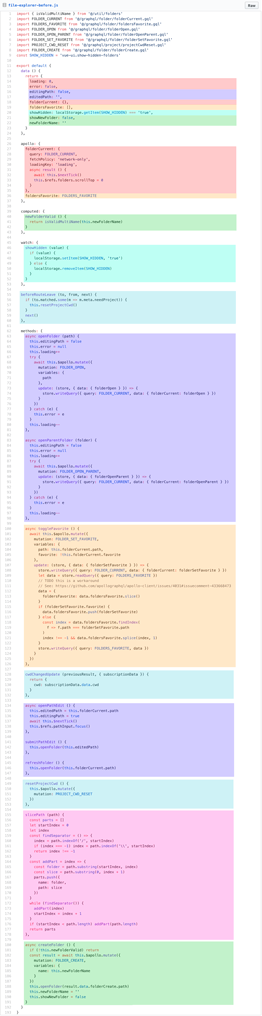
\includegraphics{./img/62783021-7ce24400-ba89-11e9-9dd3-36f4f6b1fae2.png} 
\end{center}
    

\columnratio{0.55}
\begin{paracol}{2} 
 
\switchcolumn[0]*%%%%%%%
Notice how code dealing with the same logical concern is forced to be
split under different options, located in different parts of the file.
In a component that is several hundred lines long, understanding and
navigating a single logical concern requires constantly scrolling up and
down the file, making it much more difficult than it should be. In
addition, if we ever intend to extract a logical concern into a reusable
utility, it takes quite a bit of work to find and extract the right
pieces of code from different parts of the file.
\switchcolumn
你可以看到,处理相同逻辑关注点的代码被强制拆分在了不同的选项中,位于文件的不同部分。在一个几百行的大组件中,要读懂代码中的一个逻辑关注点,需要在文件中反复上下滚动,这并不理想。另外,如果我们想要将一个逻辑关注点抽取重构到一个可复用的工具函数中,需要从文件的多个不同部分找到所需的正确片段。
\switchcolumn[0]*%%%%%%%
Here's the same component, before and after the
\href{https://gist.github.com/yyx990803/8854f8f6a97631576c14b63c8acd8f2e}{refactor
into Composition API}:
\switchcolumn
而如果\href{https://gist.github.com/yyx990803/8854f8f6a97631576c14b63c8acd8f2e}{用组合式
API 重构}这个组件,将会变成下面右边这样:
\end{paracol}

\begin{center} 
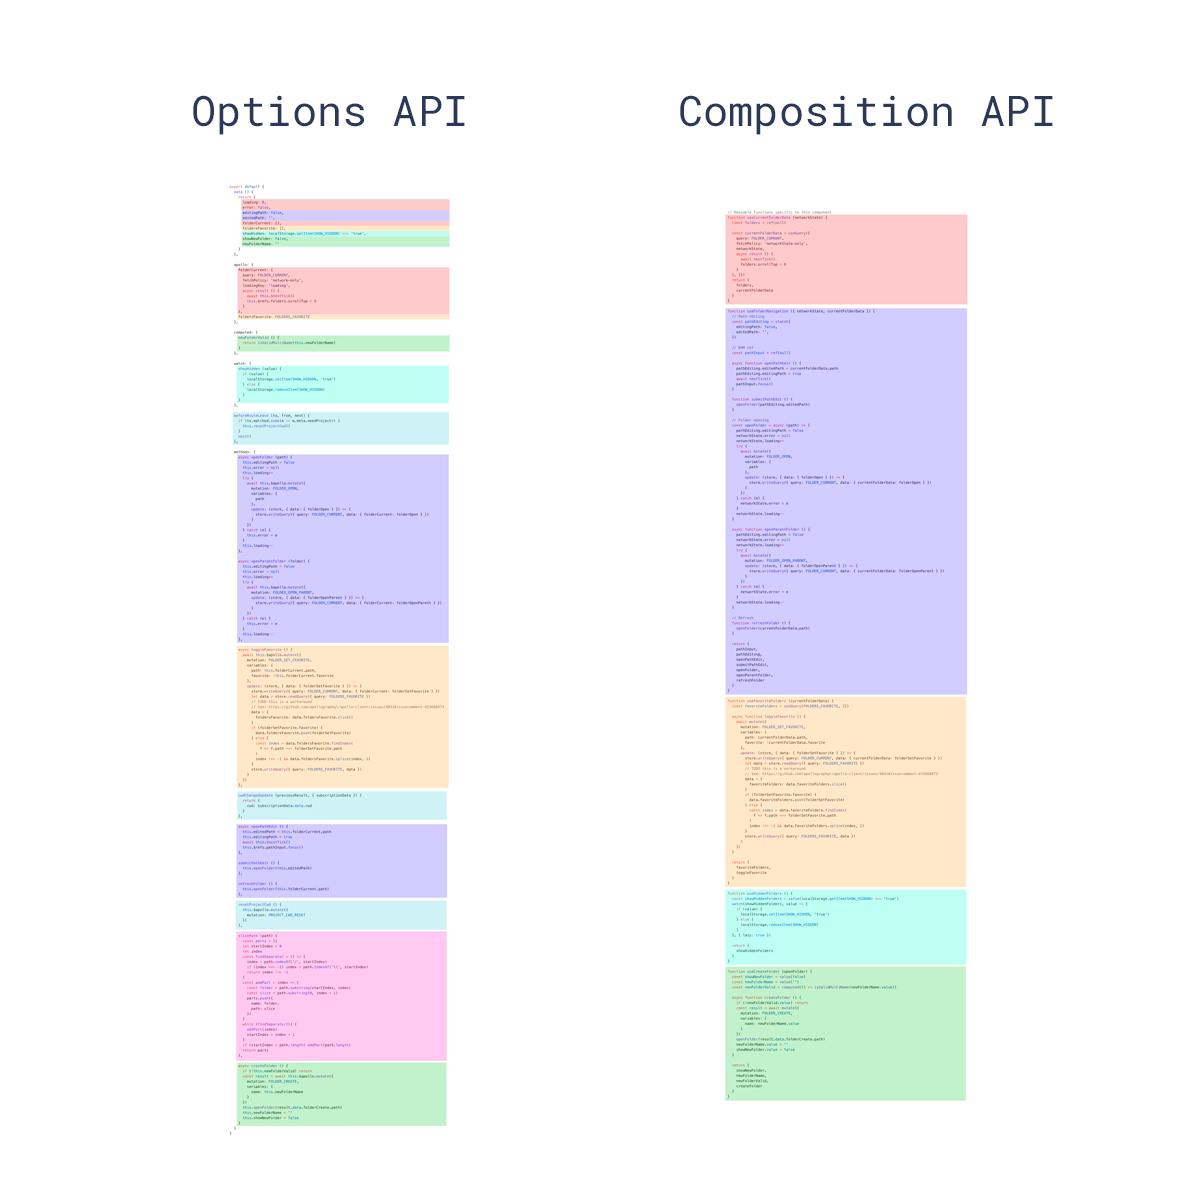
\includegraphics{./img/62783026-810e6180-ba89-11e9-8774-e7771c8095d6.png} 
\end{center}
     

\columnratio{0.55}
\begin{paracol}{2} 
 
\end{paracol}



\columnratio{0.55}
\begin{paracol}{2} 

\end{paracol}



\columnratio{0.55}
\begin{paracol}{2} 

\end{paracol}


\columnratio{0.55}
\begin{paracol}{2} 

\end{paracol}



\columnratio{0.55}
\begin{paracol}{2} 

\end{paracol}



\columnratio{0.55}
\begin{paracol}{2} 

\end{paracol}


\columnratio{0.55}
\begin{paracol}{2} 

\end{paracol}



\columnratio{0.55}
\begin{paracol}{2} 

\end{paracol}



\columnratio{0.55}
\begin{paracol}{2} 

\end{paracol}



\columnratio{0.55}
\begin{paracol}{2} 

\end{paracol}



\columnratio{0.55}
\begin{paracol}{2} 

\end{paracol}



\columnratio{0.55}
\begin{paracol}{2} 

\end{paracol}


\columnratio{0.55}
\begin{paracol}{2} 

\end{paracol}



\columnratio{0.55}
\begin{paracol}{2} 

\end{paracol}



\columnratio{0.55}
\begin{paracol}{2} 

\end{paracol}


\columnratio{0.55}
\begin{paracol}{2} 

\end{paracol}



\columnratio{0.55}
\begin{paracol}{2} 

\end{paracol}%todo 看

\columnratio{0.55}
\begin{paracol}{2} 
 
\switchcolumn[0]*%%%%%%%
\section{Reactivity in Depth}
\switchcolumn
\section{深入响应式系统}
\switchcolumn[0]*%%%%%%%
One of Vue's most distinctive features is the unobtrusive reactivity
system. Component state consists of reactive JavaScript objects. When
you modify them, the view updates. It makes state management simple and
intuitive, but it's also important to understand how it works to avoid
some common gotchas. In this section, we are going to dig into some of
the lower-level details of Vue's reactivity system.
\switchcolumn
Vue 最标志性的功能就是其低侵入性的响应式系统。组件状态都是由响应式的
JavaScript
对象组成的。当更改它们时,视图会随即自动更新。这让状态管理更加简单直观,但理解它是如何工作的也是很重要的,这可以帮助我们避免一些常见的陷阱。在本节中,我们将深入研究
Vue 响应性系统的一些底层细节。
\switchcolumn[0]*%%%%%%%
\subsection{What is Reactivity?}
\switchcolumn
\subsection{什么是响应性}
\switchcolumn[0]*%%%%%%%
This term comes up in programming quite a bit these days, but what do
people mean when they say it? Reactivity is a programming paradigm that
allows us to adjust to changes in a declarative manner. The canonical
example that people usually show, because it's a great one, is an Excel
spreadsheet:
\switchcolumn
这个术语在今天的各种编程讨论中经常出现,但人们说它的时候究竟是想表达什么意思呢?本质上,响应性是一种可以使我们声明式地处理变化的编程范式。一个经常被拿来当作典型例子的用例即是
Excel 表格:
\switchcolumn[0]*%%%%%%%
Here cell A2 is defined via a formula of \texttt{=\ A0\ +\ A1} (you can
click on A2 to view or edit the formula), so the spreadsheet gives us 3.
No surprises there. But if you update A0 or A1, you'll notice that A2
automagically updates too.
\switchcolumn
这里单元格 A2 中的值是通过公式 \texttt{=\ A0\ +\ A1} 来定义的 (你可以在
A2 上点击来查看或编辑该公式),因此最终得到的值为
3,正如所料。但如果你试着更改 A0 或 A1,你会注意到 A2 也随即自动更新了。
\switchcolumn[0]*%%%%%%%
JavaScript doesn't usually work like this. If we were to write something
comparable in JavaScript:
\switchcolumn
而 JavaScript 默认并不是这样的。如果我们用 JavaScript 写类似的逻辑:
\switchcolumn[0]*%%%%%%%
\begin{codeJs}
let A0 = 1
let A1 = 2
let A2 = A0 + A1
console.log(A2) // 3
A0 = 2
console.log(A2) // 仍然是 3
\end{codeJs}
\switchcolumn
\begin{codeJs}
let A0 = 1
let A1 = 2
let A2 = A0 + A1
console.log(A2) // 3
A0 = 2
console.log(A2) // 仍然是 3
\end{codeJs}
\switchcolumn[0]*%%%%%%%
When we mutate \texttt{A0}, \texttt{A2} does not change automatically.
\switchcolumn
当我们更改 \texttt{A0} 后,\texttt{A2} 不会自动更新。
\switchcolumn[0]*%%%%%%%
So how would we do this in JavaScript? First, in order to re-run the
code that updates \texttt{A2}, let's wrap it in a function:
\switchcolumn
那么我们如何在 JavaScript
中做到这一点呢?首先,为了能重新运行计算的代码来更新
\texttt{A2},我们需要将其包装为一个函数:
\switchcolumn[0]*%%%%%%%
\begin{codeJs}
let A2
function update() {
  A2 = A0 + A1
}
\end{codeJs}
\switchcolumn
\begin{codeJs}
let A2
function update() {
  A2 = A0 + A1
}
\end{codeJs}
\switchcolumn[0]*%%%%%%%
Then, we need to define a few terms:
\switchcolumn
然后,我们需要定义几个术语:
\switchcolumn[0]*%%%%%%%
\begin{itemize}
\item
  The \texttt{update()} function produces a \textbf{side effect}, or
  \textbf{effect} for short, because it modifies the state of the
  program.
\item
  \texttt{A0} and \texttt{A1} are considered \textbf{dependencies} of
  the effect, as their values are used to perform the effect. The effect
  is said to be a \textbf{subscriber} to its dependencies.
\end{itemize}
\switchcolumn
\begin{itemize}
\item
  这个 \texttt{update()}
  函数会产生一个\textbf{副作用},或者就简称为\textbf{作用}
  (effect),因为它会更改程序里的状态。
\item
  \texttt{A0} 和 \texttt{A1} 被视为这个作用的\textbf{依赖}
  (dependency),因为它们的值被用来执行这个作用。因此这次作用也可以说是一个它依赖的\textbf{订阅者}
  (subscriber)。
\end{itemize}
\switchcolumn[0]*%%%%%%%
What we need is a magic function that can invoke \texttt{update()} (the
\textbf{effect}) whenever \texttt{A0} or \texttt{A1} (the
\textbf{dependencies}) change:
\switchcolumn
我们需要一个魔法函数,能够在 \texttt{A0} 或 \texttt{A1}
(这两个\textbf{依赖}) 变化时调用 \texttt{update()} (产生\textbf{作用})。
\switchcolumn[0]*%%%%%%%
\begin{codeJs}
whenDepsChange(update)
\end{codeJs}
\switchcolumn
\begin{codeJs}
whenDepsChange(update)
\end{codeJs}
\switchcolumn[0]*%%%%%%%
This \texttt{whenDepsChange()} function has the following tasks:
\switchcolumn
这个 \texttt{whenDepsChange()} 函数有如下的任务:
\switchcolumn[0]*%%%%%%%
\begin{enumerate}
\item
  Track when a variable is read. E.g. when evaluating the expression
  \texttt{A0\ +\ A1}, both \texttt{A0} and \texttt{A1} are read.
\item
  If a variable is read when there is a currently running effect, make
  that effect a subscriber to that variable. E.g. because \texttt{A0}
  and \texttt{A1} are read when \texttt{update()} is being executed,
  \texttt{update()} becomes a subscriber to both \texttt{A0} and
  \texttt{A1} after the first call.
\item
  Detect when a variable is mutated. E.g. when \texttt{A0} is assigned a
  new value, notify all its subscriber effects to re-run.
\end{enumerate}
\switchcolumn
\begin{enumerate}
\item
  当一个变量被读取时进行追踪。例如我们执行了表达式 \texttt{A0\ +\ A1}
  的计算,则 \texttt{A0} 和 \texttt{A1} 都被读取到了。
\item
  如果一个变量在当前运行的副作用中被读取了,就将该副作用设为此变量的一个订阅者。例如由于
  \texttt{A0} 和 \texttt{A1} 在 \texttt{update()} 执行时被访问到了,则
  \texttt{update()} 需要在第一次调用之后成为 \texttt{A0} 和 \texttt{A1}
  的订阅者。
\item
  探测一个变量的变化。例如当我们给 \texttt{A0}
  赋了一个新的值后,应该通知其所有订阅了的副作用重新执行。
\end{enumerate}
\end{paracol}



\columnratio{0.55}
\begin{paracol}{2} 
 
\switchcolumn[0]*%%%%%%%
\subsection{How Reactivity Works in Vue}
\switchcolumn
\subsection{Vue 中的响应性是如何工作的}
\switchcolumn[0]*%%%%%%%
We can't really track the reading and writing of local variables like in
the example. There's just no mechanism for doing that in vanilla
JavaScript. What we \textbf{can} do though, is intercept the reading and
writing of \textbf{object properties}.
\switchcolumn
我们无法直接追踪对上述示例中局部变量的读写,原生 JavaScript
没有提供任何机制能做到这一点。\textbf{但是},我们是可以追踪\textbf{对象属性}的读写的。
\switchcolumn[0]*%%%%%%%
There are two ways of intercepting property access in JavaScript:
\href{https://developer.mozilla.org/en-US/docs/Web/JavaScript/Reference/Functions/get}{getter}
/
\href{https://developer.mozilla.org/en-US/docs/Web/JavaScript/Reference/Functions/set}{setters}
and
\href{https://developer.mozilla.org/en-US/docs/Web/JavaScript/Reference/Global_Objects/Proxy}{Proxies}.
Vue 2 used getter / setters exclusively due to browser support
limitations. In Vue 3, Proxies are used for reactive objects and getter
/ setters are used for refs. Here's some pseudo-code that illustrates
how they work:
\switchcolumn
在 JavaScript 中有两种劫持 property
访问的方式:\href{https://developer.mozilla.org/en-US/docs/Web/JavaScript/Reference/Functions/get}{getter}
/
\href{https://developer.mozilla.org/en-US/docs/Web/JavaScript/Reference/Functions/set}{setters}
和
\href{https://developer.mozilla.org/en-US/docs/Web/JavaScript/Reference/Global_Objects/Proxy}{Proxies}。Vue
2 使用 getter / setters 完全是出于支持旧版本浏览器的限制。而在 Vue 3
中则使用了 Proxy 来创建响应式对象,仅将 getter / setter 用于
ref。下面的伪代码将会说明它们是如何工作的:
\switchcolumn[0]*%%%%%%%
\begin{codeJs}
function reactive(obj) {
  return new Proxy(obj, {
    get(target, key) {
      track(target, key)
      return target[key]
    },
    set(target, key, value) {
      target[key] = value
      trigger(target, key)
    }
  })
}
function ref(value) {
  const refObject = {
    get value() {
      track(refObject, 'value')
      return value
    },
    set value(newValue) {
      value = newValue
      trigger(refObject, 'value')
    }
  }
  return refObject
}
\end{codeJs}
\switchcolumn
\begin{codeJs}
function reactive(obj) {
  return new Proxy(obj, {
    get(target, key) {
      track(target, key)
      return target[key]
    },
    set(target, key, value) {
      target[key] = value
      trigger(target, key)
    }
  })
}
function ref(value) {
  const refObject = {
    get value() {
      track(refObject, 'value')
      return value
    },
    set value(newValue) {
      value = newValue
      trigger(refObject, 'value')
    }
  }
  return refObject
}
\end{codeJs}
\switchcolumn[0]*%%%%%%%
\begin{vueQuote}{TIP}
Code snippets here and below are meant to explain the core concepts in
the simplest form possible, so many details are omitted, and edge cases
ignored.
\end{vueQuote} 
\switchcolumn
\begin{vueQuote}{TIP}
这里和下面的代码片段皆旨在以最简单的形式解释核心概念,因此省略了许多细节和边界情况。
\end{vueQuote} 
\switchcolumn[0]*%%%%%%%
This explains a few
\href{https://vuejs.org/guide/essentials/reactivity-fundamentals.html\#limitations-of-reactive}{limitations
of reactive objects} that we have discussed in the fundamentals section:
\switchcolumn
以上代码解释了我们在基础章节部分讨论过的一些
\href{https://cn.vuejs.org/guide/essentials/reactivity-fundamentals.html\#limitations-of-reactive}{\texttt{reactive()}
的局限性}:
\switchcolumn[0]*%%%%%%%
\begin{itemize}
\item
  When you assign or destructure a reactive object's property to a local
  variable, accessing or assigning to that variable is non-reactive
  because it no longer triggers the get / set proxy traps on the source
  object. Note this "disconnect" only affects the variable binding - if
  the variable points to a non-primitive value such as an object,
  mutating the object would still be reactive.
\item
  The returned proxy from \texttt{reactive()}, although behaving just
  like the original, has a different identity if we compare it to the
  original using the \texttt{===} operator.
\end{itemize}
\switchcolumn
\begin{itemize}
\item
  当你将一个响应式对象的属性赋值或解构到一个本地变量时,访问或赋值该变量是非响应式的,因为它将不再触发源对象上的
  get / set
  代理。注意这种``断开''只影响变量绑定------如果变量指向一个对象之类的非原始值,那么对该对象的修改仍然是响应式的。
\item
  从 \texttt{reactive()}
  返回的代理尽管行为上表现得像原始对象,但我们通过使用 \texttt{===}
  运算符还是能够比较出它们的不同。
\end{itemize}
\switchcolumn[0]*%%%%%%%
Inside \texttt{track()}, we check whether there is a currently running
effect. If there is one, we lookup the subscriber effects (stored in a
Set) for the property being tracked, and add the effect to the Set:
\switchcolumn
在 \texttt{track()}
内部,我们会检查当前是否有正在运行的副作用。如果有,我们会查找到一个存储了所有追踪了该属性的订阅者的
Set,然后将当前这个副作用作为新订阅者添加到该 Set 中。
\switchcolumn[0]*%%%%%%%
\begin{codeJs}
// 这会在一个副作用就要运行之前被设置
// 我们会在后面处理它
let activeEffect
function track(target, key) {
  if (activeEffect) {
    const effects = getSubscribersForProperty(target, key)
    effects.add(activeEffect)
  }
}
\end{codeJs}
\switchcolumn
\begin{codeJs}
// 这会在一个副作用就要运行之前被设置
// 我们会在后面处理它
let activeEffect
function track(target, key) {
  if (activeEffect) {
    const effects = getSubscribersForProperty(target, key)
    effects.add(activeEffect)
  }
}
\end{codeJs}
\switchcolumn[0]*%%%%%%%
Effect subscriptions are stored in a global
\texttt{WeakMap\textless{}target,\ Map\textless{}key,\ Set\textless{}effect\textgreater{}\textgreater{}\textgreater{}}
data structure. If no subscribing effects Set was found for a property
(tracked for the first time), it will be created. This is what the
\texttt{getSubscribersForProperty()} function does, in short. For
simplicity, we will skip its details.
\switchcolumn
副作用订阅将被存储在一个全局的
\texttt{WeakMap\textless{}target,\ Map\textless{}key,\ Set\textless{}effect\textgreater{}\textgreater{}\textgreater{}}
数据结构中。如果在第一次追踪时没有找到对相应属性订阅的副作用集合,它将会在这里新建。这就是
\texttt{getSubscribersForProperty()}
函数所做的事。为了简化描述,我们跳过了它其中的细节。
\switchcolumn[0]*%%%%%%%
Inside \texttt{trigger()}, we again lookup the subscriber effects for
the property. But this time we invoke them instead:
\switchcolumn
在 \texttt{trigger()}
之中,我们会再查找到该属性的所有订阅副作用。但这一次我们需要执行它们:
\switchcolumn[0]*%%%%%%%
\begin{codeJs}
function trigger(target, key) {
  const effects = getSubscribersForProperty(target, key)
  effects.forEach((effect) => effect())
}
\end{codeJs}
\switchcolumn
\begin{codeJs}
function trigger(target, key) {
  const effects = getSubscribersForProperty(target, key)
  effects.forEach((effect) => effect())
}
\end{codeJs}
\switchcolumn[0]*%%%%%%%
Now let's circle back to the \texttt{whenDepsChange()} function:
\switchcolumn
现在让我们回到 \texttt{whenDepsChange()} 函数中:
\switchcolumn[0]*%%%%%%%
\begin{codeJs}
function whenDepsChange(update) {
  const effect = () => {
    activeEffect = effect
    update()
    activeEffect = null
  }
  effect()
}
\end{codeJs}
\switchcolumn
\begin{codeJs}
function whenDepsChange(update) {
  const effect = () => {
    activeEffect = effect
    update()
    activeEffect = null
  }
  effect()
}
\end{codeJs}
\switchcolumn[0]*%%%%%%%
It wraps the raw \texttt{update} function in an effect that sets itself
as the current active effect before running the actual update. This
enables \texttt{track()} calls during the update to locate the current
active effect.
\switchcolumn
它将原本的 \texttt{update}
函数包装在了一个副作用函数中。在运行实际的更新之前,这个外部函数会将自己设为当前活跃的副作用。这使得在更新期间的
\texttt{track()} 调用都能定位到这个当前活跃的副作用。
\switchcolumn[0]*%%%%%%%
At this point, we have created an effect that automatically tracks its
dependencies, and re-runs whenever a dependency changes. We call this a
\textbf{Reactive Effect}.
\switchcolumn
此时,我们已经创建了一个能自动跟踪其依赖的副作用,它会在任意依赖被改动时重新运行。我们称其为\textbf{响应式副作用}。
\switchcolumn[0]*%%%%%%%
Vue provides an API that allows you to create reactive effects:
\href{https://vuejs.org/api/reactivity-core.html\#watcheffect}{\texttt{watchEffect()}}.
In fact, you may have noticed that it works pretty similarly to the
magical \texttt{whenDepsChange()} in the example. We can now rework the
original example using actual Vue APIs:
\switchcolumn
Vue 提供了一个 API 来让你创建响应式副作用
\href{https://cn.vuejs.org/api/reactivity-core.html\#watcheffect}{\texttt{watchEffect()}}。事实上,你会发现它的使用方式和我们上面示例中说的魔法函数
\texttt{whenDepsChange()} 非常相似。我们可以用真正的 Vue API
改写上面的例子:
\switchcolumn[0]*%%%%%%%
\begin{codeJs}
import { ref, watchEffect } from 'vue'
const A0 = ref(0)
const A1 = ref(1)
const A2 = ref()
watchEffect(() => {
  // 追踪 A0 和 A1
  A2.value = A0.value + A1.value
})
// 将触发副作用
A0.value = 2
\end{codeJs}
\switchcolumn
\begin{codeJs}
import { ref, watchEffect } from 'vue'
const A0 = ref(0)
const A1 = ref(1)
const A2 = ref()
watchEffect(() => {
  // 追踪 A0 和 A1
  A2.value = A0.value + A1.value
})
// 将触发副作用
A0.value = 2
\end{codeJs}
\switchcolumn[0]*%%%%%%%
Using a reactive effect to mutate a ref isn't the most interesting use
case - in fact, using a computed property makes it more declarative:
\switchcolumn
使用一个响应式副作用来更改一个 ref
并不是最优解,事实上使用计算属性会更直观简洁:
\switchcolumn[0]*%%%%%%%
\begin{codeJs}
import { ref, computed } from 'vue'
const A0 = ref(0)
const A1 = ref(1)
const A2 = computed(() => A0.value + A1.value)
A0.value = 2
\end{codeJs}
\switchcolumn
\begin{codeJs}
import { ref, computed } from 'vue'
const A0 = ref(0)
const A1 = ref(1)
const A2 = computed(() => A0.value + A1.value)
A0.value = 2
\end{codeJs}
\switchcolumn[0]*%%%%%%%
Internally, \texttt{computed} manages its invalidation and
re-computation using a reactive effect.
\switchcolumn
在内部,\texttt{computed} 会使用响应式副作用来管理失效与重新计算的过程。
\switchcolumn[0]*%%%%%%%
So what's an example of a common and useful reactive effect? Well,
updating the DOM! We can implement simple "reactive rendering" like
this:
\switchcolumn
那么,常见的响应式副作用的用例是什么呢?自然是更新
DOM!我们可以像下面这样实现一个简单的``响应式渲染'':
\switchcolumn[0]*%%%%%%%
\begin{codeJs}
import { ref, watchEffect } from 'vue'
const count = ref(0)
watchEffect(() => {
  document.body.innerHTML = `计数:${count.value}`
})
// 更新 DOM
count.value++
\end{codeJs}
\switchcolumn
\begin{codeJs}
import { ref, watchEffect } from 'vue'
const count = ref(0)
watchEffect(() => {
  document.body.innerHTML = `计数:${count.value}`
})
// 更新 DOM
count.value++
\end{codeJs}
\switchcolumn[0]*%%%%%%%
In fact, this is pretty close to how a Vue component keeps the state and
the DOM in sync - each component instance creates a reactive effect to
render and update the DOM. Of course, Vue components use much more
efficient ways to update the DOM than \texttt{innerHTML}. This is
discussed in
\href{https://vuejs.org/guide/extras/rendering-mechanism.html}{Rendering
Mechanism}.
\switchcolumn
实际上,这与 Vue 组件保持状态和 DOM
同步的方式非常接近------每个组件实例创建一个响应式副作用来渲染和更新
DOM。当然,Vue 组件使用了比 \texttt{innerHTML} 更高效的方式来更新
DOM。这会在\href{https://cn.vuejs.org/guide/extras/rendering-mechanism.html}{渲染机制}一章中详细介绍。
\end{paracol}


\columnratio{0.55}
\begin{paracol}{2} 
 
\switchcolumn[0]*%%%%%%%
\subsection{Runtime vs. Compile-time Reactivity}
\switchcolumn
\subsection{运行时 vs. 编译时响应性}
\switchcolumn[0]*%%%%%%%
Vue's reactivity system is primarily runtime-based: the tracking and
triggering are all performed while the code is running directly in the
browser. The pros of runtime reactivity are that it can work without a
build step, and there are fewer edge cases. On the other hand, this
makes it constrained by the syntax limitations of JavaScript, leading to
the need of value containers like Vue refs.
\switchcolumn
Vue
的响应式系统基本是基于运行时的。追踪和触发都是在浏览器中运行时进行的。运行时响应性的优点是,它可以在没有构建步骤的情况下工作,而且边界情况较少。另一方面,这使得它受到了
JavaScript 语法的制约,导致需要使用一些例如 Vue ref 这样的值的容器。
\switchcolumn[0]*%%%%%%%
Some frameworks, such as \href{https://svelte.dev/}{Svelte}, choose to
overcome such limitations by implementing reactivity during compilation.
It analyzes and transforms the code in order to simulate reactivity. The
compilation step allows the framework to alter the semantics of
JavaScript itself - for example, implicitly injecting code that performs
dependency analysis and effect triggering around access to locally
defined variables. The downside is that such transforms require a build
step, and altering JavaScript semantics is essentially creating a
language that looks like JavaScript but compiles into something else.
\switchcolumn
一些框架,如
\href{https://svelte.dev/}{Svelte},选择通过编译时实现响应性来克服这种限制。它对代码进行分析和转换,以模拟响应性。该编译步骤允许框架改变
JavaScript
本身的语义------例如,隐式地注入执行依赖性分析的代码,以及围绕对本地定义的变量的访问进行作用触发。这样做的缺点是,该转换需要一个构建步骤,而改变
JavaScript 的语义实质上是在创造一种新语言,看起来像 JavaScript
但编译出来的东西是另外一回事。
\switchcolumn[0]*%%%%%%%
The Vue team did explore this direction via an experimental feature
called
\href{https://vuejs.org/guide/extras/reactivity-transform.html}{Reactivity
Transform}, but in the end we have decided that it would not be a good
fit for the project due to
\href{https://github.com/vuejs/rfcs/discussions/369\#discussioncomment-5059028}{the
reasoning here}.
\switchcolumn
Vue
团队确实曾通过一个名为\href{https://cn.vuejs.org/guide/extras/reactivity-transform.html}{响应性语法糖}的实验性功能来探索这个方向,但最后由于\href{https://github.com/vuejs/rfcs/discussions/369\#discussioncomment-5059028}{这个原因},我们认为它不适合这个项目。
\switchcolumn[0]*%%%%%%%
\subsection{Reactivity Debugging}
\switchcolumn
\subsection{响应性调试}
\switchcolumn[0]*%%%%%%%
It's great that Vue's reactivity system automatically tracks
dependencies, but in some cases we may want to figure out exactly what
is being tracked, or what is causing a component to re-render.
\switchcolumn
Vue
的响应性系统可以自动跟踪依赖关系,但在某些情况下,我们可能希望确切地知道正在跟踪什么,或者是什么导致了组件重新渲染。
\end{paracol}



\columnratio{0.55}
\begin{paracol}{2} 
 
\switchcolumn[0]*%%%%%%%
\subsubsection{Component Debugging Hooks}
\switchcolumn
\subsubsection{组件调试钩子}
\switchcolumn[0]*%%%%%%%
We can debug what dependencies are used during a component's render and
which dependency is triggering an update using the
\texttt{onRenderTracked} and \texttt{onRenderTriggered} lifecycle hooks.
Both hooks will receive a debugger event which contains information on
the dependency in question. It is recommended to place a
\texttt{debugger} statement in the callbacks to interactively inspect
the dependency:
\switchcolumn
我们可以在一个组件渲染时使用 \texttt{onRenderTracked}
生命周期钩子来调试查看哪些依赖正在被使用,或是用
\texttt{onRenderTriggered}
来确定哪个依赖正在触发更新。这些钩子都会收到一个调试事件,其中包含了触发相关事件的依赖的信息。推荐在回调中放置一个
\texttt{debugger} 语句,使你可以在开发者工具中交互式地查看依赖:
\switchcolumn[0]*%%%%%%%
\begin{codeHtml}
<script setup>
import { onRenderTracked, onRenderTriggered } from 'vue'
onRenderTracked((event) => {
  debugger
})
onRenderTriggered((event) => {
  debugger
})
</script>
\end{codeHtml}
\switchcolumn
\begin{codeHtml}
<script setup>
import { onRenderTracked, onRenderTriggered } from 'vue'
onRenderTracked((event) => {
  debugger
})
onRenderTriggered((event) => {
  debugger
})
</script>
\end{codeHtml}
\switchcolumn[0]*%%%%%%%
\begin{vueQuote}{TIP}
Component debug hooks only work in development mode.
\end{vueQuote} 
\switchcolumn
\begin{vueQuote}{TIP}
组件调试钩子仅会在开发模式下工作
\end{vueQuote} 
\switchcolumn[0]*%%%%%%%
The debug event objects have the following type:
\switchcolumn
调试事件对象有如下的类型定义:
\switchcolumn[0]*%%%%%%%
\begin{codeTs}
type DebuggerEvent = {
  effect: ReactiveEffect
  target: object
  type:
    | TrackOpTypes /* 'get' | 'has' | 'iterate' */
    | TriggerOpTypes /* 'set' | 'add' | 'delete' | 'clear' */
  key: any
  newValue?: any
  oldValue?: any
  oldTarget?: Map<any, any> | Set<any>
}
\end{codeTs}
\switchcolumn
\begin{codeTs}
type DebuggerEvent = {
  effect: ReactiveEffect
  target: object
  type:
    | TrackOpTypes /* 'get' | 'has' | 'iterate' */
    | TriggerOpTypes /* 'set' | 'add' | 'delete' | 'clear' */
  key: any
  newValue?: any
  oldValue?: any
  oldTarget?: Map<any, any> | Set<any>
}
\end{codeTs}
\switchcolumn[0]*%%%%%%%
\subsubsection{Computed Debugging}
\switchcolumn
\subsubsection{计算属性调试}
\switchcolumn[0]*%%%%%%%
We can debug computed properties by passing \texttt{computed()} a second
options object with \texttt{onTrack} and \texttt{onTrigger} callbacks:
\switchcolumn
我们可以向 \texttt{computed()} 传入第二个参数,是一个包含了
\texttt{onTrack} 和 \texttt{onTrigger} 两个回调函数的对象:
\switchcolumn[0]*%%%%%%%
\begin{itemize}
\item
  \texttt{onTrack} will be called when a reactive property or ref is
  tracked as a dependency.
\item
  \texttt{onTrigger} will be called when the watcher callback is
  triggered by the mutation of a dependency.
\end{itemize}
\switchcolumn
\begin{itemize}
\item
  \texttt{onTrack} 将在响应属性或引用作为依赖项被跟踪时被调用。
\item
  \texttt{onTrigger} 将在侦听器回调被依赖项的变更触发时被调用。
\end{itemize}
\switchcolumn[0]*%%%%%%%
Both callbacks will receive debugger events in the
\href{https://vuejs.org/guide/extras/reactivity-in-depth.html\#debugger-event}{same
format} as component debug hooks:
\switchcolumn
这两个回调都会作为组件调试的钩子,接受\href{https://cn.vuejs.org/guide/extras/reactivity-in-depth.html\#debugger-event}{相同格式}的调试事件:
\switchcolumn[0]*%%%%%%%
\begin{codeJs}
const plusOne = computed(() => count.value + 1, {
  onTrack(e) {
    // 当 count.value 被追踪为依赖时触发
    debugger
  },
  onTrigger(e) {
    // 当 count.value 被更改时触发
    debugger
  }
})
// 访问 plusOne,会触发 onTrack
console.log(plusOne.value)
// 更改 count.value,应该会触发 onTrigger
count.value++
\end{codeJs}
\switchcolumn
\begin{codeJs}
const plusOne = computed(() => count.value + 1, {
  onTrack(e) {
    // 当 count.value 被追踪为依赖时触发
    debugger
  },
  onTrigger(e) {
    // 当 count.value 被更改时触发
    debugger
  }
})
// 访问 plusOne,会触发 onTrack
console.log(plusOne.value)
// 更改 count.value,应该会触发 onTrigger
count.value++
\end{codeJs}
\switchcolumn[0]*%%%%%%%
\begin{vueQuote}{TIP}
\texttt{onTrack} and \texttt{onTrigger} computed options only work in
development mode.
\end{vueQuote} 
\switchcolumn
\begin{vueQuote}{TIP}
计算属性的 \texttt{onTrack} 和 \texttt{onTrigger}
选项仅会在开发模式下工作。
\end{vueQuote} 
\end{paracol}



\columnratio{0.55}
\begin{paracol}{2} 
 
\switchcolumn[0]*%%%%%%%
\subsubsection{Watcher Debugging}
\switchcolumn
\subsubsection{侦听器调试}
\switchcolumn[0]*%%%%%%%
Similar to \texttt{computed()}, watchers also support the
\texttt{onTrack} and \texttt{onTrigger} options:
\switchcolumn
和 \texttt{computed()} 类似,侦听器也支持 \texttt{onTrack} 和
\texttt{onTrigger} 选项:

\end{paracol}

\columnratio{0.55}
\begin{paracol}{2}
\switchcolumn[0]*%%%%%%%
\begin{codeJs}
watch(source, callback, {
  onTrack(e) {
    debugger
  },
  onTrigger(e) {
    debugger
  }
})
watchEffect(callback, {
  onTrack(e) {
    debugger
  },
  onTrigger(e) {
    debugger
  }
})
\end{codeJs}
\switchcolumn
\begin{codeJs}
watch(source, callback, {
  onTrack(e) {
    debugger
  },
  onTrigger(e) {
    debugger
  }
})
watchEffect(callback, {
  onTrack(e) {
    debugger
  },
  onTrigger(e) {
    debugger
  }
})
\end{codeJs}
\end{paracol}

\columnratio{0.55}
\begin{paracol}{2}
\switchcolumn[0]*%%%%%%%
~\begin{vueQuote}{TIP}
\texttt{onTrack} and \texttt{onTrigger} watcher options only work in
development mode.
\end{vueQuote}
\switchcolumn
~\begin{vueQuote}{TIP}
侦听器的 \texttt{onTrack} 和 \texttt{onTrigger}
选项仅会在开发模式下工作。
\end{vueQuote} 
\switchcolumn[0]*%%%%%%%
\subsection{Integration with External State Systems}
\switchcolumn
\subsection{与外部状态系统集成}
\switchcolumn[0]*%%%%%%%
Vue's reactivity system works by deeply converting plain JavaScript
objects into reactive proxies. The deep conversion can be unnecessary or
sometimes unwanted when integrating with external state management
systems (e.g. if an external solution also uses Proxies).
\switchcolumn
Vue 的响应性系统是通过深度转换普通 JavaScript
对象为响应式代理来实现的。这种深度转换在一些情况下是不必要的,在和一些外部状态管理系统集成时,甚至是需要避免的
(例如,当一个外部的解决方案也用了 Proxy 时)。
\switchcolumn[0]*%%%%%%%
The general idea of integrating Vue's reactivity system with an external
state management solution is to hold the external state in a
\href{https://vuejs.org/api/reactivity-advanced.html\#shallowref}{\texttt{shallowRef}}.
A shallow ref is only reactive when its \texttt{.value} property is
accessed - the inner value is left intact. When the external state
changes, replace the ref value to trigger updates.
\switchcolumn
将 Vue
的响应性系统与外部状态管理方案集成的大致思路是:将外部状态放在一个
\href{https://cn.vuejs.org/api/reactivity-advanced.html\#shallowref}{\texttt{shallowRef}}
中。一个浅层的 ref 中只有它的 \texttt{.value}
属性本身被访问时才是有响应性的,而不关心它内部的值。当外部状态改变时,替换此
ref 的 \texttt{.value} 才会触发更新。
\switchcolumn[0]*%%%%%%%
\subsubsection{Immutable Data}
\switchcolumn
\subsubsection{不可变数据}
\switchcolumn[0]*%%%%%%%
If you are implementing an undo / redo feature, you likely want to take
a snapshot of the application's state on every user edit. However, Vue's
mutable reactivity system isn't best suited for this if the state tree
is large, because serializing the entire state object on every update
can be expensive in terms of both CPU and memory costs.
\switchcolumn
如果你正在实现一个撤销/重做的功能,你可能想要对用户编辑时应用的状态进行快照记录。然而,如果状态树很大的话,Vue
的可变响应性系统没法很好地处理这种情况,因为在每次更新时都序列化整个状态对象对
CPU 和内存开销来说都是非常昂贵的。
\switchcolumn[0]*%%%%%%%
\href{https://en.wikipedia.org/wiki/Persistent_data_structure}{Immutable
data structures} solve this by never mutating the state objects -
instead, it creates new objects that share the same, unchanged parts
with old ones. There are different ways of using immutable data in
JavaScript, but we recommend using
\href{https://immerjs.github.io/immer/}{Immer} with Vue because it
allows you to use immutable data while keeping the more ergonomic,
mutable syntax.
\switchcolumn
\href{https://en.wikipedia.org/wiki/Persistent_data_structure}{不可变数据结构}通过永不更改状态对象来解决这个问题。与
Vue 不同的是,它会创建一个新对象,保留旧的对象未发生改变的一部分。在
JavaScript 中有多种不同的方式来使用不可变数据,但我们推荐使用
\href{https://immerjs.github.io/immer/}{Immer} 搭配
Vue,因为它使你可以在保持原有直观、可变的语法的同时,使用不可变数据。
\switchcolumn[0]*%%%%%%%
We can integrate Immer with Vue via a simple composable:
\switchcolumn
我们可以通过一个简单的组合式函数来集成 Immer:
\switchcolumn[0]*%%%%%%%
\begin{codeJs}
import produce from 'immer'
import { shallowRef } from 'vue'
export function useImmer(baseState) {
  const state = shallowRef(baseState)
  const update = (updater) => {
    state.value = produce(state.value, updater)
  }
  return [state, update]
}
\end{codeJs}
\switchcolumn
\begin{codeJs}
import produce from 'immer'
import { shallowRef } from 'vue'
export function useImmer(baseState) {
  const state = shallowRef(baseState)
  const update = (updater) => {
    state.value = produce(state.value, updater)
  }
  return [state, update]
}
\end{codeJs}
\switchcolumn[0]*%%%%%%%
\href{https://play.vuejs.org/\#eNplU8Fu2zAM/RXOlzpAYu82zEu67lhgpw3bJcrBs5VYqywJkpxmMPzvoyjZNRodbJF84iOppzH7ZkxxHXhWZXvXWGE8OO4H88iU6I22HkYYHH/ue25hgrPVPTwUpQh28dc9MAXAVKOV83AUnvduC4Npa8+fg3GCw3I8PwbwGD64vPCSV8Cy77y2Cn4PnGXbFGu1wpC36EPHRO67c78cD6fgVfgOiOB9gnMtXczA1GnDFFPnQTVeaAVeXy6SSsyFavltE/OvKs+pGTg8zsxkHwl9KgIBtvbhzkl0yIWU+zIOFEeJBgKNxORoAewHSX/cSQHX3VnbA8vyMXa3pfqxb0i1CRXZWZb6w1U1snYOT40JvQ4+NVI0Lxi865NliTisMRHChOVSNaUUscCSKtyXq7LRdP6fDNvYPw3G85vftbzRtg6TrUAKxXe+s3q4dF/mQdC5bJtFTe362qB4tELVURKWAthhNc87+OhSw2V33htXleWgzMulaHQfFfj0ufhYfCpb4XySJHc9Zv7a63aQqKh0+xNRR8kiZ1K2sYhqeBI1xVHPi+xdV0upX3/w8yJ8fCiIYIrfCLPIaZH4n9rxnx7nlQQVH4YLHpTLW8YV8A0W1Ye4PO7sZiU/ylFca4mSP8yl5yvv/O4sZcSmw8/iW8bXdSTcjDiFgUz/AcH6WZQ=}{Try
it in the Playground}
\switchcolumn
\href{https://play.vuejs.org/\#eNplU8Fu2zAM/RXOlzpAYu82zEu67lhgpw3bJcrBs5VYqywJkpxmMPzvoyjZNRodbJF84iOppzH7ZkxxHXhWZXvXWGE8OO4H88iU6I22HkYYHH/ue25hgrPVPTwUpQh28dc9MAXAVKOV83AUnvduC4Npa8+fg3GCw3I8PwbwGD64vPCSV8Cy77y2Cn4PnGXbFGu1wpC36EPHRO67c78cD6fgVfgOiOB9gnMtXczA1GnDFFPnQTVeaAVeXy6SSsyFavltE/OvKs+pGTg8zsxkHwl9KgIBtvbhzkl0yIWU+zIOFEeJBgKNxORoAewHSX/cSQHX3VnbA8vyMXa3pfqxb0i1CRXZWZb6w1U1snYOT40JvQ4+NVI0Lxi865NliTisMRHChOVSNaUUscCSKtyXq7LRdP6fDNvYPw3G85vftbzRtg6TrUAKxXe+s3q4dF/mQdC5bJtFTe362qB4tELVURKWAthhNc87+OhSw2V33htXleWgzMulaHQfFfj0ufhYfCpb4XySJHc9Zv7a63aQqKh0+xNRR8kiZ1K2sYhqeBI1xVHPi+xdV0upX3/w8yJ8fCiIYIrfCLPIaZH4n9rxnx7nlQQVH4YLHpTLW8YV8A0W1Ye4PO7sZiU/ylFca4mSP8yl5yvv/O4sZcSmw8/iW8bXdSTcjDiFgUz/AcH6WZQ=}{在演练场中尝试一下}
\end{paracol}



\columnratio{0.55}
\begin{paracol}{2} 
 
\switchcolumn[0]*%%%%%%%
\subsubsection{State Machines}
\switchcolumn
\subsubsection{状态机}
\switchcolumn[0]*%%%%%%%
\href{https://en.wikipedia.org/wiki/Finite-state_machine}{State Machine}
is a model for describing all the possible states an application can be
in, and all the possible ways it can transition from one state to
another. While it may be overkill for simple components, it can help
make complex state flows more robust and manageable.
\switchcolumn
\href{https://en.wikipedia.org/wiki/Finite-state_machine}{状态机}是一种数据模型,用于描述应用可能处于的所有可能状态,以及从一种状态转换到另一种状态的所有可能方式。虽然对于简单的组件来说,这可能有些小题大做了,但它的确可以使得复杂的状态流更加健壮和易于管理。
\switchcolumn[0]*%%%%%%%
One of the most popular state machine implementations in JavaScript is
\href{https://xstate.js.org/}{XState}. Here's a composable that
integrates with it:
\switchcolumn
\href{https://xstate.js.org/}{XState} 是 JavaScript
中一个比较常用的状态机实现方案。这里是集成它的一个例子:
\switchcolumn[0]*%%%%%%%
\begin{codeJs}
import { createMachine, interpret } from 'xstate'
import { shallowRef } from 'vue'
export function useMachine(options) {
  const machine = createMachine(options)
  const state = shallowRef(machine.initialState)
  const service = interpret(machine)
    .onTransition((newState) => (state.value = newState))
    .start()
  const send = (event) => service.send(event)
  return [state, send]
}
\end{codeJs}
\switchcolumn
\begin{codeJs}
import { createMachine, interpret } from 'xstate'
import { shallowRef } from 'vue'
export function useMachine(options) {
  const machine = createMachine(options)
  const state = shallowRef(machine.initialState)
  const service = interpret(machine)
    .onTransition((newState) => (state.value = newState))
    .start()
  const send = (event) => service.send(event)
  return [state, send]
}
\end{codeJs}
\switchcolumn[0]*%%%%%%%
\href{https://play.vuejs.org/\#eNp1U81unDAQfpWRL7DSFqqqUiXEJumhyqVVpDa3ugcKZtcJjC1syEqId8/YBu/uIRcEM9/P/DGz71pn0yhYwUpTD1JbMMKO+o6j7LUaLMwwGvGrqk8SBSzQDqqHJMv7EMleTMIRgGOt0Fj4a2xlxZ5EsPkHhytuOjucbApIrDoeO5HsfQCllVVHUYlVbeW0xr2OKcCzHCwkKQAK3fP56fHx5w/irSyqbfFMgA+h0cKBHZYey45jmYfeqWv6sKLXHbnTF0D5f7RWITzUnaxfD5y5ztIkSCY7zjwKYJ5DyVlf2fokTMrZ5sbZDu6Bs6e25QwK94b0svgKyjwYkEyZR2e2Z2H8n/pK04wV0oL8KEjWJwxncTicnb23C3F2slabIs9H1K/HrFZ9HrIPX7Mv37LPuTC5xEacSfa+V83YEW+bBfleFkuW8QbqQZDEuso9rcOKQQ/CxosIHnQLkWJOVdept9+ijSA6NEJwFGePaUekAdFwr65EaRcxu9BbOKq1JDqnmzIi9oL0RRDu4p1u/ayH9schrhlimGTtOLGnjeJRAJnC56FCQ3SFaYriLWjA4Q7SsPOp6kYnEXMbldKDTW/ssCFgKiaB1kusBWT+rkLYjQiAKhkHvP2j3IqWd5iMQ+M=}{Try
it in the Playground}
\switchcolumn
\href{https://play.vuejs.org/\#eNp1U81unDAQfpWRL7DSFqqqUiXEJumhyqVVpDa3ugcKZtcJjC1syEqId8/YBu/uIRcEM9/P/DGz71pn0yhYwUpTD1JbMMKO+o6j7LUaLMwwGvGrqk8SBSzQDqqHJMv7EMleTMIRgGOt0Fj4a2xlxZ5EsPkHhytuOjucbApIrDoeO5HsfQCllVVHUYlVbeW0xr2OKcCzHCwkKQAK3fP56fHx5w/irSyqbfFMgA+h0cKBHZYey45jmYfeqWv6sKLXHbnTF0D5f7RWITzUnaxfD5y5ztIkSCY7zjwKYJ5DyVlf2fokTMrZ5sbZDu6Bs6e25QwK94b0svgKyjwYkEyZR2e2Z2H8n/pK04wV0oL8KEjWJwxncTicnb23C3F2slabIs9H1K/HrFZ9HrIPX7Mv37LPuTC5xEacSfa+V83YEW+bBfleFkuW8QbqQZDEuso9rcOKQQ/CxosIHnQLkWJOVdept9+ijSA6NEJwFGePaUekAdFwr65EaRcxu9BbOKq1JDqnmzIi9oL0RRDu4p1u/ayH9schrhlimGTtOLGnjeJRAJnC56FCQ3SFaYriLWjA4Q7SsPOp6kYnEXMbldKDTW/ssCFgKiaB1kusBWT+rkLYjQiAKhkHvP2j3IqWd5iMQ+M=}{在演练场中尝试一下}
\switchcolumn[0]*%%%%%%%
\subsubsection{RxJS}
\switchcolumn
\subsubsection{RxJS}
\switchcolumn[0]*%%%%%%%
\href{https://rxjs.dev/}{RxJS} is a library for working with
asynchronous event streams. The \href{https://vueuse.org/}{VueUse}
library provides the
\href{https://vueuse.org/rxjs/readme.html}{\texttt{@vueuse/rxjs}} add-on
for connecting RxJS streams with Vue's reactivity system.
\switchcolumn
\href{https://rxjs.dev/}{RxJS}
是一个用于处理异步事件流的库。\href{https://vueuse.org/}{VueUse}
库提供了
\href{https://vueuse.org/rxjs/readme.html}{\texttt{@vueuse/rxjs}}
扩展来支持连接 RxJS 流与 Vue 的响应性系统。
\switchcolumn[0]*%%%%%%%
\subsection{Connection to Signals}
\switchcolumn
\subsection{与信号 (signal) 的联系}
\switchcolumn[0]*%%%%%%%
Quite a few other frameworks have introduced reactivity primitives
similar to refs from Vue's Composition API, under the term "signals":
\switchcolumn
很多其他框架已经引入了与 Vue 组合式 API 中的 ref
类似的响应性基础类型,并称之为``信号'':
\switchcolumn[0]*%%%%%%%
\begin{itemize}
\item
  \href{https://www.solidjs.com/docs/latest/api\#createsignal}{Solid
  Signals}
\item
  \href{https://github.com/angular/angular/discussions/49090}{Angular
  Signals}
\item
  \href{https://preactjs.com/guide/v10/signals/}{Preact Signals}
\item
  \href{https://qwik.builder.io/docs/components/state/\#usesignal}{Qwik
  Signals}
\end{itemize}
\switchcolumn
\begin{itemize}
\item
  \href{https://www.solidjs.com/docs/latest/api\#createsignal}{Solid
  信号}
\item
  \href{https://github.com/angular/angular/discussions/49090}{Angular
  信号}
\item
  \href{https://preactjs.com/guide/v10/signals/}{Preact 信号}
\item
  \href{https://qwik.builder.io/docs/components/state/\#usesignal}{Qwik
  信号}
\end{itemize}
\switchcolumn[0]*%%%%%%%
Fundamentally, signals are the same kind of reactivity primitive as Vue
refs. It's a value container that provides dependency tracking on
access, and side-effect triggering on mutation. This
reactivity-primitive-based paradigm isn't a particularly new concept in
the frontend world: it dates back to implementations like
\href{https://knockoutjs.com/documentation/observables.html}{Knockout
observables} and \href{https://docs.meteor.com/api/tracker.html}{Meteor
Tracker} from more than a decade ago. Vue Options API and the React
state management library \href{https://mobx.js.org/}{MobX} are also
based on the same principles, but hide the primitives behind object
properties.
\switchcolumn
从根本上说,信号是与 Vue 中的 ref
相同的响应性基础类型。它是一个在访问时跟踪依赖、在变更时触发副作用的值容器。这种基于响应性基础类型的范式在前端领域并不是一个特别新的概念:它可以追溯到十多年前的
\href{https://knockoutjs.com/documentation/observables.html}{Knockout
observables} 和 \href{https://docs.meteor.com/api/tracker.html}{Meteor
Tracker} 等实现。Vue 的选项式 API 和 React 的状态管理库
\href{https://mobx.js.org/}{MobX}
也是基于同样的原则,只不过将基础类型这部分隐藏在了对象属性背后。
\switchcolumn[0]*%%%%%%%
Although not a necessary trait for something to qualify as signals,
today the concept is often discussed alongside the rendering model where
updates are performed through fine-grained subscriptions. Due to the use
of Virtual DOM, Vue currently
\href{https://vuejs.org/guide/extras/rendering-mechanism.html\#compiler-informed-virtual-dom}{relies
on compilers to achieve similar optimizations}. However, we are also
exploring a new Solid-inspired compilation strategy (Vapor Mode) that
does not rely on Virtual DOM and takes more advantage of Vue's built-in
reactivity system.
\switchcolumn
虽然这并不是信号的必要特征,但如今这个概念经常与细粒度订阅和更新的渲染模型一起讨论。由于使用了虚拟
DOM,Vue
目前\href{https://cn.vuejs.org/guide/extras/rendering-mechanism.html\#compiler-informed-virtual-dom}{依靠编译器来实现类似的优化}。然而,我们也在探索一种新的受
Solid 启发的编译策略 (Vapor Mode),它不依赖于虚拟 DOM,而是更多地利用
Vue 的内置响应性系统。
\switchcolumn[0]*%%%%%%%
\subsubsection{API Design Trade-Offs}
\switchcolumn
\subsubsection{API 设计权衡}
\switchcolumn[0]*%%%%%%%
The design of Preact and Qwik's signals are very similar to Vue's
\href{https://vuejs.org/api/reactivity-advanced.html\#shallowref}{shallowRef}:
all three provide a mutable interface via the \texttt{.value} property.
We will focus the discussion on Solid and Angular signals.
\switchcolumn
Preact 和 Qwik 的信号设计与 Vue 的
\href{https://cn.vuejs.org/api/reactivity-advanced.html\#shallowref}{shallowRef}
非常相似:三者都通过 \texttt{.value}
属性提供了一个更改接口。我们将重点讨论 Solid 和 Angular 的信号。
\switchcolumn[0]*%%%%%%%
\paragraph{Solid Signals}
\switchcolumn
\paragraph{Solid Signals}
\switchcolumn[0]*%%%%%%%
Solid's \texttt{createSignal()} API design emphasizes read / write
segregation. Signals are exposed as a read-only getter and a separate
setter:
\switchcolumn
Solid 的 \texttt{createSignal()} API
设计强调了读/写隔离。信号通过一个只读的 getter 和另一个单独的 setter
暴露:
\switchcolumn[0]*%%%%%%%
\begin{codeJs}
const [count, setCount] = createSignal(0)
count() // 访问值
setCount(1) // 更新值
\end{codeJs}
\switchcolumn
\begin{codeJs}
const [count, setCount] = createSignal(0)
count() // 访问值
setCount(1) // 更新值
\end{codeJs}
\switchcolumn[0]*%%%%%%%
Notice how the \texttt{count} signal can be passed down without the
setter. This ensures that the state can never be mutated unless the
setter is also explicitly exposed. Whether this safety guarantee
justifies the more verbose syntax could be subject to the requirement of
the project and personal taste - but in case you prefer this API style,
you can easily replicate it in Vue:
\switchcolumn
注意到 \texttt{count} 信号在没有 setter 的情况也能传递。这就保证了除非
setter
也被明确暴露,否则状态永远不会被改变。这种更冗长的语法带来的安全保证的合理性取决于项目的要求和个人品味------但如果你喜欢这种
API 风格,可以轻易地在 Vue 中复制它:
\switchcolumn[0]*%%%%%%%
\begin{codeJs}
import { shallowRef, triggerRef } from 'vue'
export function createSignal(value, options) {
  const r = shallowRef(value)
  const get = () => r.value
  const set = (v) => {
    r.value = typeof v === 'function' ? v(r.value) : v
    if (options?.equals === false) triggerRef(r)
  }
  return [get, set]
}
\end{codeJs}
\switchcolumn
\begin{codeJs}
import { shallowRef, triggerRef } from 'vue'
export function createSignal(value, options) {
  const r = shallowRef(value)
  const get = () => r.value
  const set = (v) => {
    r.value = typeof v === 'function' ? v(r.value) : v
    if (options?.equals === false) triggerRef(r)
  }
  return [get, set]
}
\end{codeJs}
\switchcolumn[0]*%%%%%%%
\href{https://play.vuejs.org/\#eNpdUk1TgzAQ/Ss7uQAjgr12oNXxH+ix9IAYaDQkMV/qMPx3N6G0Uy9Msu/tvn2PTORJqcI7SrakMp1myoKh1qldI9iopLYwQadpa+krG0TLYYZeyxGSojSSs/d7E8vFh0ka0YhOCmPh0EknbB4mPYfTEeqbIelD1oiqXPRQCS+WjoojAW8A1Wmzm1A39KYZzHNVYiUib85aKeCx46z7rBuySqQe6h14uINN1pDIBWACVUcqbGwtl17EqvIiR3LyzwcmcXFuTi3n8vuF9jlYzYaBajxfMsDcomv6E/m9E51luN2NV99yR3OQKkAmgykss+SkMZerxMLEZFZ4oBYJGAA600VEryAaD6CPaJwJKwnr9ldR2WMedV1Dsi6WwB58emZlsAV/zqmH9LzfvqBfruUmNvZ4QN7VearjenP4aHwmWsABt4x/+tiImcx/z27Jqw==}{Try
it in the Playground}
\switchcolumn
\href{https://play.vuejs.org/\#eNpdUk1TgzAQ/Ss7uQAjgr12oNXxH+ix9IAYaDQkMV/qMPx3N6G0Uy9Msu/tvn2PTORJqcI7SrakMp1myoKh1qldI9iopLYwQadpa+krG0TLYYZeyxGSojSSs/d7E8vFh0ka0YhOCmPh0EknbB4mPYfTEeqbIelD1oiqXPRQCS+WjoojAW8A1Wmzm1A39KYZzHNVYiUib85aKeCx46z7rBuySqQe6h14uINN1pDIBWACVUcqbGwtl17EqvIiR3LyzwcmcXFuTi3n8vuF9jlYzYaBajxfMsDcomv6E/m9E51luN2NV99yR3OQKkAmgykss+SkMZerxMLEZFZ4oBYJGAA600VEryAaD6CPaJwJKwnr9ldR2WMedV1Dsi6WwB58emZlsAV/zqmH9LzfvqBfruUmNvZ4QN7VearjenP4aHwmWsABt4x/+tiImcx/z27Jqw==}{在演练场中尝试一下}
\switchcolumn[0]*%%%%%%%
\paragraph{Angular Signals}
\switchcolumn
\paragraph{Angular 信号}
\switchcolumn[0]*%%%%%%%
Angular is undergoing some fundamental changes by foregoing
dirty-checking and introducing its own implementation of a reactivity
primitive. The Angular Signal API looks like this:
\switchcolumn
Angular
正在经历一些底层的变化,它放弃了脏检查,并引入了自己的响应性基础类型实现。Angular
的信号 API 看起来像这样:
\switchcolumn[0]*%%%%%%%
\begin{codeJs}
const count = signal(0)
count() // 访问值
count.set(1) //设置值
count.update((v) => v + 1) // 通过前值更新
// 对具有相同身份的深层对象进行更改
const state = signal({ count: 0 })
state.mutate((o) => {
  o.count++
})
\end{codeJs}
\switchcolumn
\begin{codeJs}
const count = signal(0)
count() // 访问值
count.set(1) //设置值
count.update((v) => v + 1) // 通过前值更新
// 对具有相同身份的深层对象进行更改
const state = signal({ count: 0 })
state.mutate((o) => {
  o.count++
})
\end{codeJs}
\switchcolumn[0]*%%%%%%%
Again, we can easily replicate the API in Vue:
\switchcolumn
同样,我们可以轻易地在 Vue 中复制这个 API:
\switchcolumn[0]*%%%%%%%
\begin{codeJs}
import { shallowRef, triggerRef } from 'vue'
export function signal(initialValue) {
  const r = shallowRef(initialValue)
  const s = () => r.value
  s.set = (value) => {
    r.value = value
  }
  s.update = (updater) => {
    r.value = updater(r.value)
  }
  s.mutate = (mutator) => {
    mutator(r.value)
    triggerRef(r)
  }
  return s
}
\end{codeJs}
\switchcolumn
\begin{codeJs}
import { shallowRef, triggerRef } from 'vue'
export function signal(initialValue) {
  const r = shallowRef(initialValue)
  const s = () => r.value
  s.set = (value) => {
    r.value = value
  }
  s.update = (updater) => {
    r.value = updater(r.value)
  }
  s.mutate = (mutator) => {
    mutator(r.value)
    triggerRef(r)
  }
  return s
}
\end{codeJs}
\switchcolumn[0]*%%%%%%%
\href{https://play.vuejs.org/\#eNp9UslOwzAQ/ZVRLiRQEsqxpBUIvoADp0goTd3U4DiWl4AU5d8ZL3E3iZtn5r1Z3vOYvAiRD4Ykq6RUjaRCgyLaiE3FaSd6qWEERVteswU0fSeMJjuYYC/7Dm7youatYbW895D8S91UvOJNz5VGuOEa1oGePmRzYdebLSNYmRumaQbrjSfg8xYeEVsWfh/cBANNOsFqTTACKA/LzavrTtUKxjEyp6kssDZj3vygAPJjL1Bbo3XP4blhtPleV4nrlBuxw1npYLca4A6WWZU4PADljSQd4drRC8//rxfKaW+f+ZJg4oJbFvG8ZJFcaYreHL041Iz1P+9kvwAtadsS6d7Rm1rB55VRaLAzhvy6NnvDG01x1WAN5VTTmn3UzJAMRrudd0pa++LEc9wRpRDlHZT5YGu2pOzhWHAJWxvnakxOHufFxqx/4MxzcEinIYP+eV5ntOe5Rx94IYjopxOZUhnIEr+4xPMrjuG1LPFftkTj5DNJGhwYBZ4BJz3DV56FmJLpD1DrKXU=}{Try
it in the Playground}
\switchcolumn
\href{https://play.vuejs.org/\#eNp9UslOwzAQ/ZVRLiRQEsqxpBUIvoADp0goTd3U4DiWl4AU5d8ZL3E3iZtn5r1Z3vOYvAiRD4Ykq6RUjaRCgyLaiE3FaSd6qWEERVteswU0fSeMJjuYYC/7Dm7youatYbW895D8S91UvOJNz5VGuOEa1oGePmRzYdebLSNYmRumaQbrjSfg8xYeEVsWfh/cBANNOsFqTTACKA/LzavrTtUKxjEyp6kssDZj3vygAPJjL1Bbo3XP4blhtPleV4nrlBuxw1npYLca4A6WWZU4PADljSQd4drRC8//rxfKaW+f+ZJg4oJbFvG8ZJFcaYreHL041Iz1P+9kvwAtadsS6d7Rm1rB55VRaLAzhvy6NnvDG01x1WAN5VTTmn3UzJAMRrudd0pa++LEc9wRpRDlHZT5YGu2pOzhWHAJWxvnakxOHufFxqx/4MxzcEinIYP+eV5ntOe5Rx94IYjopxOZUhnIEr+4xPMrjuG1LPFftkTj5DNJGhwYBZ4BJz3DV56FmJLpD1DrKXU=}{在演练场中尝试一下}
\switchcolumn[0]*%%%%%%%
Compared to Vue refs, Solid and Angular's getter-based API style provide
some interesting trade-offs when used in Vue components:
\switchcolumn
与 Vue 的 ref 相比,Solid 和 Angular 基于 getter 的 API 风格在 Vue
组件中使用时提供了一些有趣的权衡:
\switchcolumn[0]*%%%%%%%
\begin{itemize}
\item
  \texttt{()} is slightly less verbose than \texttt{.value}, but
  updating the value is more verbose.
\item
  There is no ref-unwrapping: accessing values always require
  \texttt{()}. This makes value access consistent everywhere. This also
  means you can pass raw signals down as component props.
\end{itemize}
\switchcolumn
\begin{itemize}
\item
  \texttt{()} 比 \texttt{.value} 略微省事,但更新值却更冗长;
\item
  没有 ref 解包:总是需要通过 \texttt{()}
  来访问值。这使得值的访问在任何地方都是一致的。这也意味着你可以将原始信号作为组件的参数传递下去。
\end{itemize}
\switchcolumn[0]*%%%%%%%
Whether these API styles suit you is to some extent subjective. Our goal
here is to demonstrate the underlying similarity and trade-offs between
these different API designs. We also want to show that Vue is flexible:
you are not really locked into the existing APIs. Should it be
necessary, you can create your own reactivity primitive API to suit more
specific needs.
\switchcolumn
这些 API
风格是否适合你,在某种程度上是主观的。我们在这里的目标是展示这些不同的
API 设计之间的基本相似性和取舍。我们还想说明 Vue
是灵活的:你并没有真正被限定在现有的 API
中。如有必要,你可以创建你自己的响应性基础 API,以满足更多的具体需求。
\end{paracol}

 %todo 看

\columnratio{0.55}
\begin{paracol}{2} 
 
\switchcolumn[0]*%%%%%%%
\section{Rendering Mechanism}
\switchcolumn
\section{渲染机制}
\switchcolumn[0]*%%%%%%%
How does Vue take a template and turn it into actual DOM nodes? How does
Vue update those DOM nodes efficiently? We will attempt to shed some
light on these questions here by diving into Vue's internal rendering
mechanism.
\switchcolumn
Vue 是如何将一份模板转换为真实的 DOM
节点的,又是如何高效地更新这些节点的呢?我们接下来就将尝试通过深入研究
Vue 的内部渲染机制来解释这些问题。
\switchcolumn[0]*%%%%%%%
\subsection{Virtual DOM}
\switchcolumn
\subsection{虚拟 DOM}
\switchcolumn[0]*%%%%%%%
You have probably heard about the term "virtual DOM", which Vue's
rendering system is based upon.
\switchcolumn
你可能已经听说过``虚拟 DOM''的概念了,Vue
的渲染系统正是基于这个概念构建的。
\switchcolumn[0]*%%%%%%%
The virtual DOM (VDOM) is a programming concept where an ideal, or
``virtual'', representation of a UI is kept in memory and synced with
the ``real'' DOM. The concept was pioneered by
\href{https://reactjs.org/}{React}, and has been adopted in many other
frameworks with different implementations, including Vue.
\switchcolumn
虚拟 DOM (Virtual DOM,简称 VDOM) 是一种编程概念,意为将目标所需的 UI
通过数据结构``虚拟''地表示出来,保存在内存中,然后将真实的 DOM
与之保持同步。这个概念是由 \href{https://reactjs.org/}{React}
率先开拓,随后被许多不同的框架采用,当然也包括 Vue。
\switchcolumn[0]*%%%%%%%
Virtual DOM is more of a pattern than a specific technology, so there is
no one canonical implementation. We can illustrate the idea using a
simple example:
\switchcolumn
与其说虚拟 DOM
是一种具体的技术,不如说是一种模式,所以并没有一个标准的实现。我们可以用一个简单的例子来说明:
\switchcolumn[0]*%%%%%%%
\begin{codeJs}
const vnode = {
  type: 'div',
  props: {
    id: 'hello'
  },
  children: [
    /* 更多 vnode */
  ]
}
\end{codeJs}
\switchcolumn
\begin{codeJs}
const vnode = {
  type: 'div',
  props: {
    id: 'hello'
  },
  children: [
    /* 更多 vnode */
  ]
}
\end{codeJs}
\switchcolumn[0]*%%%%%%%
Here, \texttt{vnode} is a plain JavaScript object (a "virtual node")
representing a \texttt{\textless{}div\textgreater{}} element. It
contains all the information that we need to create the actual element.
It also contains more children vnodes, which makes it the root of a
virtual DOM tree.
\switchcolumn
这里所说的 \texttt{vnode} 即一个纯 JavaScript 的对象
(一个``虚拟节点''),它代表着一个 \texttt{\textless{}div\textgreater{}}
元素。它包含我们创建实际元素所需的所有信息。它还包含更多的子节点,这使它成为虚拟
DOM 树的根节点。
\switchcolumn[0]*%%%%%%%
A runtime renderer can walk a virtual DOM tree and construct a real DOM
tree from it. This process is called \textbf{mount}.
\switchcolumn
一个运行时渲染器将会遍历整个虚拟 DOM 树,并据此构建真实的 DOM
树。这个过程被称为\textbf{挂载} (mount)。
\switchcolumn[0]*%%%%%%%
If we have two copies of virtual DOM trees, the renderer can also walk
and compare the two trees, figuring out the differences, and apply those
changes to the actual DOM. This process is called \textbf{patch}, also
known as "diffing" or "reconciliation".
\switchcolumn
如果我们有两份虚拟 DOM
树,渲染器将会有比较地遍历它们,找出它们之间的区别,并应用这其中的变化到真实的
DOM 上。这个过程被称为\textbf{更新} (patch),又被称为``比对''(diffing)
或``协调''(reconciliation)。
\switchcolumn[0]*%%%%%%%
The main benefit of virtual DOM is that it gives the developer the
ability to programmatically create, inspect and compose desired UI
structures in a declarative way, while leaving the direct DOM
manipulation to the renderer.
\switchcolumn
虚拟 DOM
带来的主要收益是它让开发者能够灵活、声明式地创建、检查和组合所需 UI
的结构,同时只需把具体的 DOM 操作留给渲染器去处理。
\end{paracol}



\columnratio{0.55}
\begin{paracol}{2} 
 
\switchcolumn[0]*%%%%%%%
\subsection{Render Pipeline}
\switchcolumn
\subsection{渲染管线}
\switchcolumn[0]*%%%%%%%
At the high level, this is what happens when a Vue component is mounted:
\switchcolumn
从高层面的视角看,Vue 组件挂载时会发生如下几件事:
\switchcolumn[0]*%%%%%%%
\begin{enumerate}
\item
  \textbf{Compile}: Vue templates are compiled into \textbf{render
  functions}: functions that return virtual DOM trees. This step can be
  done either ahead-of-time via a build step, or on-the-fly by using the
  runtime compiler.
\item
  \textbf{Mount}: The runtime renderer invokes the render functions,
  walks the returned virtual DOM tree, and creates actual DOM nodes
  based on it. This step is performed as a
  \href{https://vuejs.org/guide/extras/reactivity-in-depth.html}{reactive
  effect}, so it keeps track of all reactive dependencies that were
  used.
\item
  \textbf{Patch}: When a dependency used during mount changes, the
  effect re-runs. This time, a new, updated Virtual DOM tree is created.
  The runtime renderer walks the new tree, compares it with the old one,
  and applies necessary updates to the actual DOM.
\end{enumerate}
\switchcolumn
\begin{enumerate}
\item
  \textbf{编译}:Vue 模板被编译为\textbf{渲染函数}:即用来返回虚拟 DOM
  树的函数。这一步骤可以通过构建步骤提前完成,也可以通过使用运行时编译器即时完成。
\item
  \textbf{挂载}:运行时渲染器调用渲染函数,遍历返回的虚拟 DOM
  树,并基于它创建实际的 DOM
  节点。这一步会作为\href{https://cn.vuejs.org/guide/extras/reactivity-in-depth.html}{响应式副作用}执行,因此它会追踪其中所用到的所有响应式依赖。
\item
  \textbf{更新}:当一个依赖发生变化后,副作用会重新运行,这时候会创建一个更新后的虚拟
  DOM
  树。运行时渲染器遍历这棵新树,将它与旧树进行比较,然后将必要的更新应用到真实
  DOM 上去。
\end{enumerate}
\end{paracol}

\begin{center} 
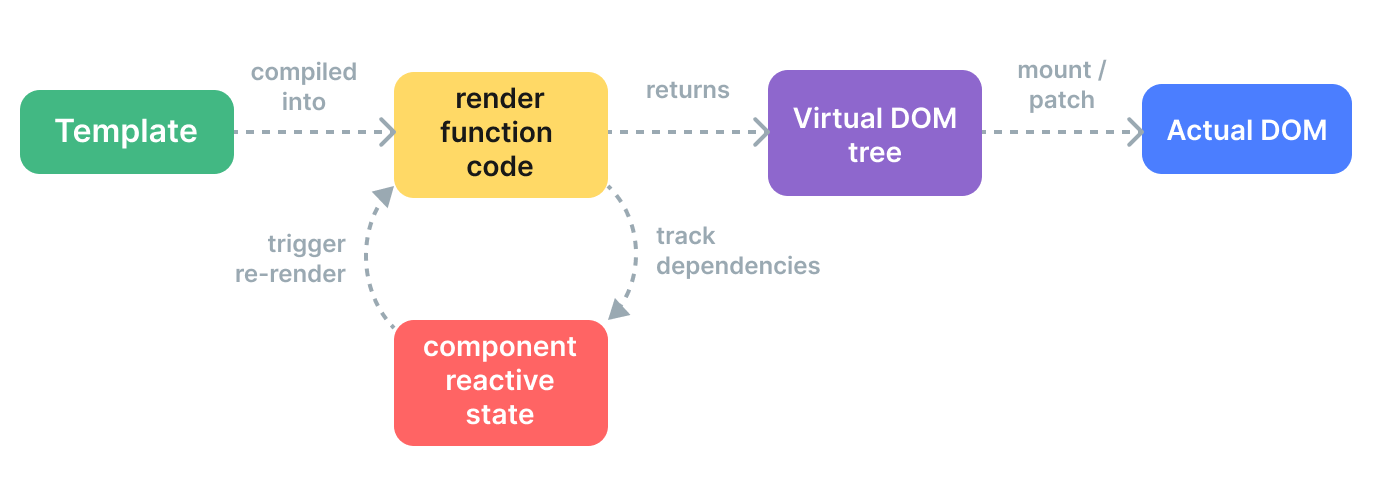
\includegraphics{./img/render-pipeline.03805016.png} 
\end{center}
    

\columnratio{0.55}
\begin{paracol}{2} 
 
\switchcolumn[0]*%%%%%%%
\subsection{Templates vs. Render Functions}
\switchcolumn
\subsection{模板 vs. 渲染函数}
\switchcolumn[0]*%%%%%%%
Vue templates are compiled into virtual DOM render functions. Vue also
provides APIs that allow us to skip the template compilation step and
directly author render functions. Render functions are more flexible
than templates when dealing with highly dynamic logic, because you can
work with vnodes using the full power of JavaScript.
\switchcolumn
Vue 模板会被预编译成虚拟 DOM 渲染函数。Vue 也提供了 API
使我们可以不使用模板编译,直接手写渲染函数。在处理高度动态的逻辑时,渲染函数相比于模板更加灵活,因为你可以完全地使用
JavaScript 来构造你想要的 vnode。
\switchcolumn[0]*%%%%%%%
So why does Vue recommend templates by default? There are a number of
reasons:
\switchcolumn
那么为什么 Vue 默认推荐使用模板呢?有以下几点原因:
\switchcolumn[0]*%%%%%%%
\begin{enumerate}
\def\labelenumi{\arabic{enumi}.}
\item
  Templates are closer to actual HTML. This makes it easier to reuse
  existing HTML snippets, apply accessibility best practices, style with
  CSS, and for designers to understand and modify.
\item
  Templates are easier to statically analyze due to their more
  deterministic syntax. This allows Vue's template compiler to apply
  many compile-time optimizations to improve the performance of the
  virtual DOM (which we will discuss below).
\end{enumerate}
\switchcolumn
\begin{enumerate}
\def\labelenumi{\arabic{enumi}.}
\item
  模板更贴近实际的 HTML。这使得我们能够更方便地重用一些已有的 HTML
  代码片段,能够带来更好的可访问性体验、能更方便地使用 CSS
  应用样式,并且更容易使设计师理解和修改。
\item
  由于其确定的语法,更容易对模板做静态分析。这使得 Vue
  的模板编译器能够应用许多编译时优化来提升虚拟 DOM 的性能表现
  (下面我们将展开讨论)。
\end{enumerate}
\switchcolumn[0]*%%%%%%%
In practice, templates are sufficient for most use cases in
applications. Render functions are typically only used in reusable
components that need to deal with highly dynamic rendering logic. Render
function usage is discussed in more detail in
\href{https://vuejs.org/guide/extras/render-function.html}{Render
Functions \& JSX}.
\switchcolumn
在实践中,模板对大多数的应用场景都是够用且高效的。渲染函数一般只会在需要处理高度动态渲染逻辑的可重用组件中使用。想了解渲染函数的更多使用细节可以去到\href{https://cn.vuejs.org/guide/extras/render-function.html}{渲染函数
\& JSX} 章节继续阅读。
\switchcolumn[0]*%%%%%%%
\subsection{Compiler-Informed Virtual DOM}
\switchcolumn
\subsection{带编译时信息的虚拟 DOM}
\switchcolumn[0]*%%%%%%%
The virtual DOM implementation in React and most other virtual-DOM
implementations are purely runtime: the reconciliation algorithm cannot
make any assumptions about the incoming virtual DOM tree, so it has to
fully traverse the tree and diff the props of every vnode in order to
ensure correctness. In addition, even if a part of the tree never
changes, new vnodes are always created for them on each re-render,
resulting in unnecessary memory pressure. This is one of the most
criticized aspect of virtual DOM: the somewhat brute-force
reconciliation process sacrifices efficiency in return for
declarativeness and correctness.
\switchcolumn
虚拟 DOM 在 React
和大多数其他实现中都是纯运行时的:更新算法无法预知新的虚拟 DOM
树会是怎样,因此它总是需要遍历整棵树、比较每个 vnode 上 props
的区别来确保正确性。另外,即使一棵树的某个部分从未改变,还是会在每次重渲染时创建新的
vnode,带来了大量不必要的内存压力。这也是虚拟 DOM
最受诟病的地方之一:这种有点暴力的更新过程通过牺牲效率来换取声明式的写法和最终的正确性。
\switchcolumn[0]*%%%%%%%
But it doesn't have to be that way. In Vue, the framework controls both
the compiler and the runtime. This allows us to implement many
compile-time optimizations that only a tightly-coupled renderer can take
advantage of. The compiler can statically analyze the template and leave
hints in the generated code so that the runtime can take shortcuts
whenever possible. At the same time, we still preserve the capability
for the user to drop down to the render function layer for more direct
control in edge cases. We call this hybrid approach
\textbf{Compiler-Informed Virtual DOM}.
\switchcolumn
但实际上我们并不需要这样。在 Vue
中,框架同时控制着编译器和运行时。这使得我们可以为紧密耦合的模板渲染器应用许多编译时优化。编译器可以静态分析模板并在生成的代码中留下标记,使得运行时尽可能地走捷径。与此同时,我们仍旧保留了边界情况时用户想要使用底层渲染函数的能力。我们称这种混合解决方案为\textbf{带编译时信息的虚拟
DOM}。
\switchcolumn[0]*%%%%%%%
Below, we will discuss a few major optimizations done by the Vue
template compiler to improve the virtual DOM's runtime performance.
\switchcolumn
下面,我们将讨论一些 Vue 编译器用来提高虚拟 DOM 运行时性能的主要优化:
\switchcolumn[0]*%%%%%%%
\subsubsection{Static Hoisting}
\switchcolumn
\subsubsection{静态提升}
\switchcolumn[0]*%%%%%%%
Quite often there will be parts in a template that do not contain any
dynamic bindings:
\switchcolumn
在模板中常常有部分内容是不带任何动态绑定的:
\switchcolumn[0]*%%%%%%%
\begin{codeHtml}
<div>
  <div>foo</div> <!-- 需提升 -->
  <div>bar</div> <!-- 需提升 -->
  <div>{{ dynamic }}</div>
</div>
\end{codeHtml}
\switchcolumn
\begin{codeHtml}
<div>
  <div>foo</div> <!-- 需提升 -->
  <div>bar</div> <!-- 需提升 -->
  <div>{{ dynamic }}</div>
</div>
\end{codeHtml}
\switchcolumn[0]*%%%%%%%
\href{https://template-explorer.vuejs.org/\#eyJzcmMiOiI8ZGl2PlxuICA8ZGl2PmZvbzwvZGl2PiA8IS0tIGhvaXN0ZWQgLS0+XG4gIDxkaXY+YmFyPC9kaXY+IDwhLS0gaG9pc3RlZCAtLT5cbiAgPGRpdj57eyBkeW5hbWljIH19PC9kaXY+XG48L2Rpdj5cbiIsIm9wdGlvbnMiOnsiaG9pc3RTdGF0aWMiOnRydWV9fQ==}{Inspect
in Template Explorer}
\switchcolumn
\href{https://template-explorer.vuejs.org/\#eyJzcmMiOiI8ZGl2PlxuICA8ZGl2PmZvbzwvZGl2PiA8IS0tIGhvaXN0ZWQgLS0+XG4gIDxkaXY+YmFyPC9kaXY+IDwhLS0gaG9pc3RlZCAtLT5cbiAgPGRpdj57eyBkeW5hbWljIH19PC9kaXY+XG48L2Rpdj5cbiIsIm9wdGlvbnMiOnsiaG9pc3RTdGF0aWMiOnRydWV9fQ==}{在模板编译预览中查看}
\switchcolumn[0]*%%%%%%%
The \texttt{foo} and \texttt{bar} divs are static - re-creating vnodes
and diffing them on each re-render is unnecessary. The Vue compiler
automatically hoists their vnode creation calls out of the render
function, and reuses the same vnodes on every render. The renderer is
also able to completely skip diffing them when it notices the old vnode
and the new vnode are the same one.
\switchcolumn
\texttt{foo} 和 \texttt{bar} 这两个 div
是完全静态的,没有必要在重新渲染时再次创建和比对它们。Vue
编译器自动地会提升这部分 vnode
创建函数到这个模板的渲染函数之外,并在每次渲染时都使用这份相同的
vnode,渲染器知道新旧 vnode
在这部分是完全相同的,所以会完全跳过对它们的差异比对。
\switchcolumn[0]*%%%%%%%
In addition, when there are enough consecutive static elements, they
will be condensed into a single "static vnode" that contains the plain
HTML string for all these nodes
(\href{https://template-explorer.vuejs.org/\#eyJzcmMiOiI8ZGl2PlxuICA8ZGl2IGNsYXNzPVwiZm9vXCI+Zm9vPC9kaXY+XG4gIDxkaXYgY2xhc3M9XCJmb29cIj5mb288L2Rpdj5cbiAgPGRpdiBjbGFzcz1cImZvb1wiPmZvbzwvZGl2PlxuICA8ZGl2IGNsYXNzPVwiZm9vXCI+Zm9vPC9kaXY+XG4gIDxkaXYgY2xhc3M9XCJmb29cIj5mb288L2Rpdj5cbiAgPGRpdj57eyBkeW5hbWljIH19PC9kaXY+XG48L2Rpdj4iLCJzc3IiOmZhbHNlLCJvcHRpb25zIjp7ImhvaXN0U3RhdGljIjp0cnVlfX0=}{Example}).
These static vnodes are mounted by directly setting \texttt{innerHTML}.
They also cache their corresponding DOM nodes on initial mount - if the
same piece of content is reused elsewhere in the app, new DOM nodes are
created using native \texttt{cloneNode()}, which is extremely efficient.
\switchcolumn
此外,当有足够多连续的静态元素时,它们还会再被压缩为一个``静态
vnode'',其中包含的是这些节点相应的纯 HTML
字符串。(\href{https://template-explorer.vuejs.org/\#eyJzcmMiOiI8ZGl2PlxuICA8ZGl2IGNsYXNzPVwiZm9vXCI+Zm9vPC9kaXY+XG4gIDxkaXYgY2xhc3M9XCJmb29cIj5mb288L2Rpdj5cbiAgPGRpdiBjbGFzcz1cImZvb1wiPmZvbzwvZGl2PlxuICA8ZGl2IGNsYXNzPVwiZm9vXCI+Zm9vPC9kaXY+XG4gIDxkaXYgY2xhc3M9XCJmb29cIj5mb288L2Rpdj5cbiAgPGRpdj57eyBkeW5hbWljIH19PC9kaXY+XG48L2Rpdj4iLCJzc3IiOmZhbHNlLCJvcHRpb25zIjp7ImhvaXN0U3RhdGljIjp0cnVlfX0=}{示例})。这些静态节点会直接通过
\texttt{innerHTML} 来挂载。同时还会在初次挂载后缓存相应的 DOM
节点。如果这部分内容在应用中其他地方被重用,那么将会使用原生的
\texttt{cloneNode()} 方法来克隆新的 DOM 节点,这会非常高效。
\end{paracol}


\columnratio{0.55}
\begin{paracol}{2} 
 
\switchcolumn[0]*%%%%%%%
\subsubsection{Patch Flags}
\switchcolumn
\subsubsection{更新类型标记}
\switchcolumn[0]*%%%%%%%
For a single element with dynamic bindings, we can also infer a lot of
information from it at compile time:
\switchcolumn
对于单个有动态绑定的元素来说,我们可以在编译时推断出大量信息:
\switchcolumn[0]*%%%%%%%
\begin{codeHtml}
<!-- 仅含 class 绑定 -->
<div :class="{ active }"></div>
<!-- 仅含 id 和 value 绑定 -->
<input :id="id" :value="value">
<!-- 仅含文本子节点 -->
<div>{{ dynamic }}</div>
\end{codeHtml}
\switchcolumn
\begin{codeHtml}
<!-- 仅含 class 绑定 -->
<div :class="{ active }"></div>
<!-- 仅含 id 和 value 绑定 -->
<input :id="id" :value="value">
<!-- 仅含文本子节点 -->
<div>{{ dynamic }}</div>
\end{codeHtml}
\switchcolumn[0]*%%%%%%%
\href{https://template-explorer.vuejs.org/\#eyJzcmMiOiI8ZGl2IDpjbGFzcz1cInsgYWN0aXZlIH1cIj48L2Rpdj5cblxuPGlucHV0IDppZD1cImlkXCIgOnZhbHVlPVwidmFsdWVcIj5cblxuPGRpdj57eyBkeW5hbWljIH19PC9kaXY+Iiwib3B0aW9ucyI6e319}{Inspect
in Template Explorer}
\switchcolumn
\href{https://template-explorer.vuejs.org/\#eyJzcmMiOiI8ZGl2IDpjbGFzcz1cInsgYWN0aXZlIH1cIj48L2Rpdj5cblxuPGlucHV0IDppZD1cImlkXCIgOnZhbHVlPVwidmFsdWVcIj5cblxuPGRpdj57eyBkeW5hbWljIH19PC9kaXY+Iiwib3B0aW9ucyI6e319}{在模板编译预览中查看}
\switchcolumn[0]*%%%%%%%
When generating the render function code for these elements, Vue encodes
the type of update each of them needs directly in the vnode creation
call:
\switchcolumn
在为这些元素生成渲染函数时,Vue 在 vnode
创建调用中直接编码了每个元素所需的更新类型:
\switchcolumn[0]*%%%%%%%
\begin{codeJs}
createElementVNode("div", {
  class: _normalizeClass({ active: _ctx.active })
}, null, 2 /* CLASS */)
\end{codeJs}
\switchcolumn
\begin{codeJs}
createElementVNode("div", {
  class: _normalizeClass({ active: _ctx.active })
}, null, 2 /* CLASS */)
\end{codeJs}
\switchcolumn[0]*%%%%%%%
The last argument, \texttt{2}, is a
\href{https://github.com/vuejs/core/blob/main/packages/shared/src/patchFlags.ts}{patch
flag}. An element can have multiple patch flags, which will be merged
into a single number. The runtime renderer can then check against the
flags using
\href{https://en.wikipedia.org/wiki/Bitwise_operation}{bitwise
operations} to determine whether it needs to do certain work:
\switchcolumn
最后这个参数 \texttt{2}
就是一个\href{https://github.com/vuejs/core/blob/main/packages/shared/src/patchFlags.ts}{更新类型标记
(patch
flag)}。一个元素可以有多个更新类型标记,会被合并成一个数字。运行时渲染器也将会使用\href{https://en.wikipedia.org/wiki/Bitwise_operation}{位运算}来检查这些标记,确定相应的更新操作:
\switchcolumn[0]*%%%%%%%
\begin{codeJs}
if (vnode.patchFlag & PatchFlags.CLASS /* 2 */) {
  // 更新节点的 CSS class
}
\end{codeJs}
\switchcolumn
\begin{codeJs}
if (vnode.patchFlag & PatchFlags.CLASS /* 2 */) {
  // 更新节点的 CSS class
}
\end{codeJs}
\switchcolumn[0]*%%%%%%%
Bitwise checks are extremely fast. With the patch flags, Vue is able to
do the least amount of work necessary when updating elements with
dynamic bindings.
\switchcolumn
位运算检查是非常快的。通过这样的更新类型标记,Vue
能够在更新带有动态绑定的元素时做最少的操作。
\switchcolumn[0]*%%%%%%%
Vue also encodes the type of children a vnode has. For example, a
template that has multiple root nodes is represented as a fragment. In
most cases, we know for sure that the order of these root nodes will
never change, so this information can also be provided to the runtime as
a patch flag:
\switchcolumn
Vue 也为 vnode
的子节点标记了类型。举例来说,包含多个根节点的模板被表示为一个片段
(fragment),大多数情况下,我们可以确定其顺序是永远不变的,所以这部分信息就可以提供给运行时作为一个更新类型标记。
\switchcolumn[0]*%%%%%%%
\begin{codeJs}
export function render() {
  return (_openBlock(), _createElementBlock(_Fragment, null, [
    /* children */
  ], 64 /* STABLE_FRAGMENT */))
}
\end{codeJs}
\switchcolumn
\begin{codeJs}
export function render() {
  return (_openBlock(), _createElementBlock(_Fragment, null, [
    /* children */
  ], 64 /* STABLE_FRAGMENT */))
}
\end{codeJs}
\switchcolumn[0]*%%%%%%%
The runtime can thus completely skip child-order reconciliation for the
root fragment.
\switchcolumn
运行时会完全跳过对这个根片段中子元素顺序的重新协调过程。
\switchcolumn[0]*%%%%%%%
\subsubsection{Tree Flattening}
\switchcolumn
\subsubsection{树结构打平}
\switchcolumn[0]*%%%%%%%
Taking another look at the generated code from the previous example,
you'll notice the root of the returned virtual DOM tree is created using
a special \texttt{createElementBlock()} call:
\switchcolumn
再来看看上面这个例子中生成的代码,你会发现所返回的虚拟 DOM
树是经一个特殊的 \texttt{createElementBlock()} 调用创建的:
\switchcolumn[0]*%%%%%%%
\begin{codeJs}
export function render() {
  return (_openBlock(), _createElementBlock(_Fragment, null, [
    /* children */
  ], 64 /* STABLE_FRAGMENT */))
}
\end{codeJs}
\switchcolumn
\begin{codeJs}
export function render() {
  return (_openBlock(), _createElementBlock(_Fragment, null, [
    /* children */
  ], 64 /* STABLE_FRAGMENT */))
}
\end{codeJs}
\switchcolumn[0]*%%%%%%%
Conceptually, a "block" is a part of the template that has stable inner
structure. In this case, the entire template has a single block because
it does not contain any structural directives like \texttt{v-if} and
\texttt{v-for}.
\switchcolumn
这里我们引入一个概念``区块'',内部结构是稳定的一个部分可被称之为一个区块。在这个用例中,整个模板只有一个区块,因为这里没有用到任何结构性指令
(比如 \texttt{v-if} 或者 \texttt{v-for})。
\switchcolumn[0]*%%%%%%%
Each block tracks any descendant nodes (not just direct children) that
have patch flags. For example:
\switchcolumn
每一个块都会追踪其所有带更新类型标记的后代节点
(不只是直接子节点),举例来说:
\switchcolumn[0]*%%%%%%%
\begin{codeHtml}
<div> <!-- root block -->
  <div>...</div>         <!-- 不会追踪 -->
  <div :id="id"></div>   <!-- 要追踪 -->
  <div>                  <!-- 不会追踪 -->
    <div>{{ bar }}</div> <!-- 要追踪 -->
  </div>
</div>
\end{codeHtml}
\switchcolumn
\begin{codeHtml}
<div> <!-- root block -->
  <div>...</div>         <!-- 不会追踪 -->
  <div :id="id"></div>   <!-- 要追踪 -->
  <div>                  <!-- 不会追踪 -->
    <div>{{ bar }}</div> <!-- 要追踪 -->
  </div>
</div>
\end{codeHtml}
\switchcolumn[0]*%%%%%%%
The result is a flattened array that contains only the dynamic
descendant nodes:
\switchcolumn
编译的结果会被打平为一个数组,仅包含所有动态的后代节点:
\switchcolumn[0]*%%%%%%%
\begin{codeHtml}
div (block root)
- div 带有 :id 绑定
- div 带有 {{ bar }} 绑定
\end{codeHtml}
\switchcolumn
\begin{codeHtml}
div (block root)
- div 带有 :id 绑定
- div 带有 {{ bar }} 绑定
\end{codeHtml}
\switchcolumn[0]*%%%%%%%
When this component needs to re-render, it only needs to traverse the
flattened tree instead of the full tree. This is called \textbf{Tree
Flattening}, and it greatly reduces the number of nodes that need to be
traversed during virtual DOM reconciliation. Any static parts of the
template are effectively skipped.
\switchcolumn
当这个组件需要重渲染时,只需要遍历这个打平的树而非整棵树。这也就是我们所说的\textbf{树结构打平},这大大减少了我们在虚拟
DOM 协调时需要遍历的节点数量。模板中任何的静态部分都会被高效地略过。
\switchcolumn[0]*%%%%%%%
\texttt{v-if} and \texttt{v-for} directives will create new block nodes:
\switchcolumn
\texttt{v-if} 和 \texttt{v-for} 指令会创建新的区块节点:
\switchcolumn[0]*%%%%%%%
\begin{codeHtml}
<div> <!-- 根区块 -->
  <div>
    <div v-if> <!-- if 区块 -->
      ...
    <div>
  </div>
</div>
\end{codeHtml}
\switchcolumn
\begin{codeHtml}
<div> <!-- 根区块 -->
  <div>
    <div v-if> <!-- if 区块 -->
      ...
    <div>
  </div>
</div>
\end{codeHtml}
\switchcolumn[0]*%%%%%%%
A child block is tracked inside the parent block's array of dynamic
descendants. This retains a stable structure for the parent block.
\switchcolumn
一个子区块会在父区块的动态子节点数组中被追踪,这为他们的父区块保留了一个稳定的结构。
\end{paracol}



\columnratio{0.55}
\begin{paracol}{2} 
 
\switchcolumn[0]*%%%%%%%
\subsubsection{Impact on SSR Hydration}
\switchcolumn
\subsubsection{对 SSR 激活的影响}
\switchcolumn[0]*%%%%%%%
Both patch flags and tree flattening also greatly improve Vue's
\href{https://vuejs.org/guide/scaling-up/ssr.html\#client-hydration}{SSR
Hydration} performance:
\switchcolumn
更新类型标记和树结构打平都大大提升了 Vue
\href{https://cn.vuejs.org/guide/scaling-up/ssr.html\#client-hydration}{SSR
激活}的性能表现:
\switchcolumn[0]*%%%%%%%
\begin{itemize}
\item
  Single element hydration can take fast paths based on the
  corresponding vnode's patch flag.
\item
  Only block nodes and their dynamic descendants need to be traversed
  during hydration, effectively achieving partial hydration at the
  template level.
\end{itemize}
\switchcolumn
\begin{itemize}
\item
  单个元素的激活可以基于相应 vnode 的更新类型标记走更快的捷径。
\item
  在激活时只有区块节点和其动态子节点需要被遍历,这在模板层面上实现更高效的部分激活。
\end{itemize}
\end{paracol}

%todo 看 

\columnratio{0.55}
\begin{paracol}{2} 
 
\switchcolumn[0]*%%%%%%%
\section{Render Functions \& JSX}
\switchcolumn
\section{渲染函数 \& JSX}
\switchcolumn[0]*%%%%%%%
Vue recommends using templates to build applications in the vast
majority of cases. However, there are situations where we need the full
programmatic power of JavaScript. That's where we can use the
\textbf{render function}.
\switchcolumn
在绝大多数情况下,Vue
推荐使用模板语法来创建应用。然而在某些使用场景下,我们真的需要用到
JavaScript 完全的编程能力。这时\textbf{渲染函数}就派上用场了。
\switchcolumn[0]*%%%%%%%
\begin{quote}
If you are new to the concept of virtual DOM and render functions, make
sure to read the
\href{https://vuejs.org/guide/extras/rendering-mechanism.html}{Rendering
Mechanism} chapter first.
\end{quote}
\switchcolumn
\begin{quote}
如果你还不熟悉虚拟 DOM
和渲染函数的概念的话,请确保先阅读\href{https://cn.vuejs.org/guide/extras/rendering-mechanism.html}{渲染机制}章节。
\end{quote}
\switchcolumn[0]*%%%%%%%
\subsection{Basic Usage}
\switchcolumn
\subsection{基本用法}
\switchcolumn[0]*%%%%%%%
\subsubsection{Creating Vnodes}
\switchcolumn
\subsubsection{创建 Vnodes}
\switchcolumn[0]*%%%%%%%
Vue provides an \texttt{h()} function for creating vnodes:
\switchcolumn
Vue 提供了一个 \texttt{h()} 函数用于创建 vnodes:
\switchcolumn[0]*%%%%%%%
\begin{codeJs}
import { h } from 'vue'
const vnode = h(
  'div', // type
  { id: 'foo', class: 'bar' }, // props
  [
    /* children */
  ]
)
\end{codeJs}
\switchcolumn
\begin{codeJs}
import { h } from 'vue'
const vnode = h(
  'div', // type
  { id: 'foo', class: 'bar' }, // props
  [
    /* children */
  ]
)
\end{codeJs}
\switchcolumn[0]*%%%%%%%
\texttt{h()} is short for \textbf{hyperscript} - which means "JavaScript
that produces HTML (hypertext markup language)". This name is inherited
from conventions shared by many virtual DOM implementations. A more
descriptive name could be \texttt{createVnode()}, but a shorter name
helps when you have to call this function many times in a render
function.
\switchcolumn
\texttt{h()} 是 \textbf{hyperscript} 的简称------意思是``能生成 HTML
(超文本标记语言) 的 JavaScript''。这个名字来源于许多虚拟 DOM
实现默认形成的约定。一个更准确的名称应该是
\texttt{createVnode()},但当你需要多次使用渲染函数时,一个简短的名字会更省力。
\switchcolumn[0]*%%%%%%%
The \texttt{h()} function is designed to be very flexible:
\switchcolumn
\texttt{h()} 函数的使用方式非常的灵活:
\switchcolumn[0]*%%%%%%%
\begin{codeJs}
// 除了类型必填以外,其他的参数都是可选的
h('div')
h('div', { id: 'foo' })
// attribute 和 property 都能在 prop 中书写
// Vue 会自动将它们分配到正确的位置
h('div', { class: 'bar', innerHTML: 'hello' })
// 像 `.prop` 和 `.attr` 这样的的属性修饰符
// 可以分别通过 `.` 和 `^` 前缀来添加
h('div', { '.name': 'some-name', '^width': '100' })
// 类与样式可以像在模板中一样
// 用数组或对象的形式书写
h('div', { class: [foo, { bar }], style: { color: 'red' } })
// 事件监听器应以 onXxx 的形式书写
h('div', { onClick: () => {} })
// children 可以是一个字符串
h('div', { id: 'foo' }, 'hello')
// 没有 props 时可以省略不写
h('div', 'hello')
h('div', [h('span', 'hello')])
// children 数组可以同时包含 vnodes 与字符串
h('div', ['hello', h('span', 'hello')])
\end{codeJs}
\switchcolumn
\begin{codeJs}
// 除了类型必填以外,其他的参数都是可选的
h('div')
h('div', { id: 'foo' })
// attribute 和 property 都能在 prop 中书写
// Vue 会自动将它们分配到正确的位置
h('div', { class: 'bar', innerHTML: 'hello' })
// 像 `.prop` 和 `.attr` 这样的的属性修饰符
// 可以分别通过 `.` 和 `^` 前缀来添加
h('div', { '.name': 'some-name', '^width': '100' })
// 类与样式可以像在模板中一样
// 用数组或对象的形式书写
h('div', { class: [foo, { bar }], style: { color: 'red' } })
// 事件监听器应以 onXxx 的形式书写
h('div', { onClick: () => {} })
// children 可以是一个字符串
h('div', { id: 'foo' }, 'hello')
// 没有 props 时可以省略不写
h('div', 'hello')
h('div', [h('span', 'hello')])
// children 数组可以同时包含 vnodes 与字符串
h('div', ['hello', h('span', 'hello')])
\end{codeJs}
\switchcolumn[0]*%%%%%%%
The resulting vnode has the following shape:
\switchcolumn
得到的 vnode 为如下形式:
\switchcolumn[0]*%%%%%%%
\begin{codeJs}
const vnode = h('div', { id: 'foo' }, [])
vnode.type // 'div'
vnode.props // { id: 'foo' }
vnode.children // []
vnode.key // null
\end{codeJs}
\switchcolumn
\begin{codeJs}
const vnode = h('div', { id: 'foo' }, [])
vnode.type // 'div'
vnode.props // { id: 'foo' }
vnode.children // []
vnode.key // null
\end{codeJs}
\switchcolumn[0]*%%%%%%%
\begin{vueQuoteWarn}{Note}
The full \texttt{VNode} interface contains many other internal
properties, but it is strongly recommended to avoid relying on any
properties other than the ones listed here. This avoids unintended
breakage in case the internal properties are changed.
\end{vueQuoteWarn}
\switchcolumn
\begin{vueQuoteWarn}{注意事项}
完整的 \texttt{VNode}
接口包含其他内部属性,但是强烈建议避免使用这些没有在这里列举出的属性。这样能够避免因内部属性变更而导致的不兼容性问题。
\end{vueQuoteWarn}
\switchcolumn[0]*%%%%%%%
\subsubsection{Declaring Render Functions}
\switchcolumn
\subsubsection{声明渲染函数}
\switchcolumn[0]*%%%%%%%
When using templates with Composition API, the return value of the
\texttt{setup()} hook is used to expose data to the template. When using
render functions, however, we can directly return the render function
instead:
\switchcolumn
当组合式 API 与模板一起使用时,\texttt{setup()}
钩子的返回值是用于暴露数据给模板。然而当我们使用渲染函数时,可以直接把渲染函数返回:
\switchcolumn[0]*%%%%%%%
\begin{codeJs}
import { ref, h } from 'vue'
export default {
  props: {
    /* ... */
  },
  setup(props) {
    const count = ref(1)
    // 返回渲染函数
    return () => h('div', props.msg + count.value)
  }
}
\end{codeJs}
\switchcolumn
\begin{codeJs}
import { ref, h } from 'vue'
export default {
  props: {
    /* ... */
  },
  setup(props) {
    const count = ref(1)
    // 返回渲染函数
    return () => h('div', props.msg + count.value)
  }
}
\end{codeJs}
\switchcolumn[0]*%%%%%%%
The render function is declared inside \texttt{setup()} so it naturally
has access to the props and any reactive state declared in the same
scope.
\switchcolumn
在 \texttt{setup()} 内部声明的渲染函数天生能够访问在同一范围内声明的
props 和许多响应式状态。
\switchcolumn[0]*%%%%%%%
In addition to returning a single vnode, you can also return strings or
arrays:
\switchcolumn
除了返回一个 vnode,你还可以返回字符串或数组:
\switchcolumn[0]*%%%%%%%
\begin{codeJs}
export default {
  setup() {
    return () => 'hello world!'
  }
}
\end{codeJs}
\switchcolumn
\begin{codeJs}
export default {
  setup() {
    return () => 'hello world!'
  }
}
\end{codeJs}
\switchcolumn[0]*%%%%%%%
\begin{codeJs}
import { h } from 'vue'
export default {
  setup() {
    // 使用数组返回多个根节点
    return () => [
      h('div'),
      h('div'),
      h('div')
    ]
  }
}
\end{codeJs}
\switchcolumn
\begin{codeJs}
import { h } from 'vue'
export default {
  setup() {
    // 使用数组返回多个根节点
    return () => [
      h('div'),
      h('div'),
      h('div')
    ]
  }
}
\end{codeJs}
\switchcolumn[0]*%%%%%%%
\begin{vueQuote}{TIP}
Make sure to return a function instead of directly returning values! The
\texttt{setup()} function is called only once per component, while the
returned render function will be called multiple times.
\end{vueQuote} 
\switchcolumn
\begin{vueQuote}{TIP}
请确保返回的是一个函数而不是一个值!\texttt{setup()}
函数在每个组件中只会被调用一次,而返回的渲染函数将会被调用多次。
\end{vueQuote} 
\switchcolumn[0]*%%%%%%%
If a render function component doesn't need any instance state, they can
also be declared directly as a function for brevity:
\switchcolumn
如果一个渲染函数组件不需要任何实例状态,为了简洁起见,它们也可以直接被声明为一个函数:
\switchcolumn[0]*%%%%%%%
\begin{codeJs}
function Hello() {
  return 'hello world!'
}
\end{codeJs}
\switchcolumn
\begin{codeJs}
function Hello() {
  return 'hello world!'
}
\end{codeJs}
\switchcolumn[0]*%%%%%%%
That's right, this is a valid Vue component! See
\href{https://vuejs.org/guide/extras/render-function.html\#functional-components}{Functional
Components} for more details on this syntax.
\switchcolumn
没错,这就是一个合法的 Vue
组件!参阅\href{https://cn.vuejs.org/guide/extras/render-function.html\#functional-components}{函数式组件}来了解更多语法细节。
\end{paracol}



\columnratio{0.55}
\begin{paracol}{2} 
 
\switchcolumn[0]*%%%%%%%
\subsubsection{Vnodes Must Be Unique}
\switchcolumn
\subsubsection{Vnodes 必须唯一}
\switchcolumn[0]*%%%%%%%
All vnodes in the component tree must be unique. That means the
following render function is invalid:
\switchcolumn
组件树中的 vnodes 必须是唯一的。下面是错误示范:
\switchcolumn[0]*%%%%%%%
\begin{codeJs}
function render() {
  const p = h('p', 'hi')
  return h('div', [
    // 啊哦,重复的 vnodes 是无效的
    p,
    p
  ])
}
\end{codeJs}
\switchcolumn
\begin{codeJs}
function render() {
  const p = h('p', 'hi')
  return h('div', [
    // 啊哦,重复的 vnodes 是无效的
    p,
    p
  ])
}
\end{codeJs}
\switchcolumn[0]*%%%%%%%
If you really want to duplicate the same element/component many times,
you can do so with a factory function. For example, the following render
function is a perfectly valid way of rendering 20 identical paragraphs:
\switchcolumn
如果你真的非常想在页面上渲染多个重复的元素或者组件,你可以使用一个工厂函数来做这件事。比如下面的这个渲染函数就可以完美渲染出
20 个相同的段落:
\switchcolumn[0]*%%%%%%%
\begin{codeJs}
function render() {
  return h(
    'div',
    Array.from({ length: 20 }).map(() => {
      return h('p', 'hi')
    })
  )
}
\end{codeJs}
\switchcolumn
\begin{codeJs}
function render() {
  return h(
    'div',
    Array.from({ length: 20 }).map(() => {
      return h('p', 'hi')
    })
  )
}
\end{codeJs}
\switchcolumn[0]*%%%%%%%
\subsection{JSX / TSX}
\switchcolumn
\subsection{JSX / TSX}
\switchcolumn[0]*%%%%%%%
\href{https://facebook.github.io/jsx/}{JSX} is an XML-like extension to
JavaScript that allows us to write code like this:
\switchcolumn
\href{https://facebook.github.io/jsx/}{JSX} 是 JavaScript 的一个类似 XML
的扩展,有了它,我们可以用以下的方式来书写代码:
\switchcolumn[0]*%%%%%%%
%todo jsx
\begin{codeHtml}
const vnode = <div>hello</div>
\end{codeHtml}
\switchcolumn
%todo jsx
\begin{codeHtml}
const vnode = <div>hello</div>
\end{codeHtml}
\switchcolumn[0]*%%%%%%%
Inside JSX expressions, use curly braces to embed dynamic values:
\switchcolumn
在 JSX 表达式中,使用大括号来嵌入动态值:
\end{paracol}


\columnratio{0.55}
\begin{paracol}{2}  

\switchcolumn[0]*%%%%%%%
%jsx
\begin{codeHtml}
const vnode = <div id={dynamicId}>hello, {userName}</div>
\end{codeHtml}
\texttt{create-vue} and Vue CLI both have options for scaffolding
projects with pre-configured JSX support. If you are configuring JSX
manually, please refer to the documentation of
\href{https://github.com/vuejs/jsx-next}{\texttt{@vue/babel-plugin-jsx}}
for details.
\switchcolumn
%jsx
\begin{codeHtml}
const vnode = <div id={dynamicId}>hello, {userName}</div>
\end{codeHtml}
\texttt{create-vue} 和 Vue CLI 都有预置的 JSX 语法支持。如果你想手动配置
JSX,请参阅
\href{https://github.com/vuejs/jsx-next}{\texttt{@vue/babel-plugin-jsx}}
文档获取更多细节。
\switchcolumn[0]*%%%%%%%
Although first introduced by React, JSX actually has no defined runtime
semantics and can be compiled into various different outputs. If you
have worked with JSX before, do note that \textbf{Vue JSX transform is
different from React's JSX transform}, so you can't use React's JSX
transform in Vue applications. Some notable differences from React JSX
include:
\switchcolumn
虽然最早是由 React 引入,但实际上 JSX
语法并没有定义运行时语义,并且能被编译成各种不同的输出形式。如果你之前使用过
JSX 语法,那么请注意 \textbf{Vue 的 JSX 转换方式与 React 中 JSX
的转换方式不同},因此你不能在 Vue 应用中使用 React 的 JSX 转换。与 React
JSX 语法的一些明显区别包括:
\switchcolumn[0]*%%%%%%%
\begin{itemize}
\item
    You can use HTML attributes such as \texttt{class} and \texttt{for} as
    props - no need to use \texttt{className} or \texttt{htmlFor}.
\item
    Passing children to components (i.e. slots)
    \href{https://vuejs.org/guide/extras/render-function.html\#passing-slots}{works
differently}.
\end{itemize}
\switchcolumn
\begin{itemize}
\item
    可以使用 HTML attributes 比如 \texttt{class} 和 \texttt{for} 作为
    props - 不需要使用 \texttt{className} 或 \texttt{htmlFor}。
\item
    传递子元素给组件 (比如 slots)
    的\href{https://cn.vuejs.org/guide/extras/render-function.html\#passing-slots}{方式不同}。
\end{itemize}
\switchcolumn[0]*%%%%%%%
Vue's type definition also provides type inference for TSX usage. When
using TSX, make sure to specify \texttt{"jsx":\ "preserve"} in
\texttt{tsconfig.json} so that TypeScript leaves the JSX syntax intact
for Vue JSX transform to process.
\switchcolumn
Vue 的类型定义也提供了 TSX 语法的类型推导支持。当使用 TSX 语法时,确保在
\texttt{tsconfig.json} 中配置了 \texttt{"jsx":\ "preserve"},这样的
TypeScript 就能保证 Vue JSX 语法转换过程中的完整性。
\switchcolumn[0]*%%%%%%%
\subsubsection{JSX Type Inference}
\switchcolumn
\subsubsection{JSX 类型推断}
\switchcolumn[0]*%%%%%%%
Similar to the transform, Vue's JSX also needs different type
definitions. Currently, Vue's types automatically registers Vue's JSX
types globally. This means TSX will work out of the box when Vue's type
is available.
\switchcolumn
与转换类似,Vue 的 JSX 也需要不同的类型定义。目前,Vue
的类型会在全局范围内自动注册 Vue 的 JSX 类型。这意味着当 Vue
的类型可用时,TSX 将可以开箱即用。
\switchcolumn[0]*%%%%%%%
The global JSX types may cause conflict with used together with other
libraries that also needs JSX type inference, in particular React.
Starting in 3.3, Vue supports specifying JSX namespace via TypeScript's
\href{https://www.typescriptlang.org/tsconfig\#jsxImportSource}{jsxImportSource}
option. We plan to remove the default global JSX namespace registration
in 3.4.
\switchcolumn
全局的 JSX 类型在与其他同样需要 JSX
类型推断的库一起使用时可能会引起冲突,特别是 React。从 3.3 开始,Vue
支持通过 TypeScript 的
\href{https://www.typescriptlang.org/tsconfig\#jsxImportSource}{jsxImportSource}
选项指定 JSX 命名空间。我们计划在 3.4 中移除默认的全局 JSX
命名空间注册。
\switchcolumn[0]*%%%%%%%
For TSX users, it is suggested to set
\href{https://www.typescriptlang.org/tsconfig\#jsxImportSource}{jsxImportSource}
to \texttt{\textquotesingle{}vue\textquotesingle{}} in
\texttt{tsconfig.json} after upgrading to 3.3, or opt-in per file with
\texttt{/*\ @jsxImportSource\ vue\ */}. This will allow you to opt-in to
the new behavior now and upgrade seamlessly when 3.4 releases.
\switchcolumn
对于 TSX 用户,建议在升级到 3.3 之后,在 \texttt{tsconfig.json} 中把
\href{https://www.typescriptlang.org/tsconfig\#jsxImportSource}{jsxImportSource}
设置为
\texttt{\textquotesingle{}vue\textquotesingle{}},或者针对单个文件加入
\texttt{/*\ @jsxImportSource\ vue\ */}。这可以让你现在就选用该新特性,并在
3.4 发布时无痛升级。
\switchcolumn[0]*%%%%%%%
If there is code that depends on the presence of the global \texttt{JSX}
namespace, you can retain the exact pre-3.4 global behavior by
explicitly referencing \texttt{vue/jsx}, which registers the global
\texttt{JSX} namespace.
\switchcolumn
如果仍有代码依赖于全局存在的 \texttt{JSX} 命名空间,你可以通过显式引用
\texttt{vue/jsx} 来保留 3.4 之前的全局行为,它注册了全局 \texttt{JSX}
命名空间。
\end{paracol}



\columnratio{0.55}
\begin{paracol}{2} 
 
\switchcolumn[0]*%%%%%%%
\subsection{Render Function Recipes}
\switchcolumn
\subsection{渲染函数案例}
\switchcolumn[0]*%%%%%%%
Below we will provide some common recipes for implementing template
features as their equivalent render functions / JSX.
\switchcolumn
下面我们提供了几个常见的用等价的渲染函数 / JSX
语法,实现模板功能的案例:
\switchcolumn[0]*%%%%%%%
\subsubsection{v-if}
\switchcolumn
\subsubsection{v-if}
\switchcolumn[0]*%%%%%%%
Template:
\switchcolumn
模板:
\switchcolumn[0]*%%%%%%%
\begin{codeHtml}
<div>
  <div v-if="ok">yes</div>
  <span v-else>no</span>
</div>
\end{codeHtml}
\switchcolumn
\begin{codeHtml}
<div>
  <div v-if="ok">yes</div>
  <span v-else>no</span>
</div>
\end{codeHtml}
\switchcolumn[0]*%%%%%%%
Equivalent render function / JSX:
\switchcolumn
等价于使用如下渲染函数 / JSX 语法:
\switchcolumn[0]*%%%%%%%
\begin{codeJs}
h('div', [ok.value ? h('div', 'yes') : h('span', 'no')])
\end{codeJs}
\switchcolumn
\begin{codeJs}
h('div', [ok.value ? h('div', 'yes') : h('span', 'no')])
\end{codeJs}
\switchcolumn[0]*%%%%%%%
\begin{codeHtml}
<div>{ok.value ? <div>yes</div> : <span>no</span>}</div>
\end{codeHtml}
\switchcolumn
\begin{codeHtml}
<div>{ok.value ? <div>yes</div> : <span>no</span>}</div>
\end{codeHtml}
\switchcolumn[0]*%%%%%%%
\subsubsection{v-for}
\switchcolumn
\subsubsection{v-for}
\switchcolumn[0]*%%%%%%%
Template:
\switchcolumn
模板:
\switchcolumn[0]*%%%%%%%
\begin{codeHtml}
<ul>
  <li v-for="{ id, text } in items" :key="id">
    {{ text }}
  </li>
</ul>
\end{codeHtml}
\switchcolumn
\begin{codeHtml}
<ul>
  <li v-for="{ id, text } in items" :key="id">
    {{ text }}
  </li>
</ul>
\end{codeHtml}
\switchcolumn[0]*%%%%%%%
Equivalent render function / JSX:
\switchcolumn
等价于使用如下渲染函数 / JSX 语法:
\switchcolumn[0]*%%%%%%%
\begin{codeJs}
h(
  'ul',
  // assuming `items` is a ref with array value
  items.value.map(({ id, text }) => {
    return h('li', { key: id }, text)
  })
)
\end{codeJs}
\switchcolumn
\begin{codeJs}
h(
  'ul',
  // assuming `items` is a ref with array value
  items.value.map(({ id, text }) => {
    return h('li', { key: id }, text)
  })
)
\end{codeJs}
\switchcolumn[0]*%%%%%%%
\begin{codeHtml}
<ul>
  {items.value.map(({ id, text }) => {
    return <li key={id}>{text}</li>
  })}
</ul>
\end{codeHtml}
\switchcolumn
\begin{codeHtml}
<ul>
  {items.value.map(({ id, text }) => {
    return <li key={id}>{text}</li>
  })}
</ul>
\end{codeHtml}
\switchcolumn[0]*%%%%%%%
\subsubsection{v-on}
\switchcolumn
\subsubsection{v-on}
\switchcolumn[0]*%%%%%%%
Props with names that start with \texttt{on} followed by an uppercase
letter are treated as event listeners. For example, \texttt{onClick} is
the equivalent of \texttt{@click} in templates.
\switchcolumn
以 \texttt{on} 开头,并跟着大写字母的 props
会被当作事件监听器。比如,\texttt{onClick} 与模板中的 \texttt{@click}
等价。
\switchcolumn[0]*%%%%%%%
\begin{codeJs}
h(
  'button',
  {
    onClick(event) {
      /* ... */
    }
  },
  'click me'
)
\end{codeJs}
\switchcolumn
\begin{codeJs}
h(
  'button',
  {
    onClick(event) {
      /* ... */
    }
  },
  'click me'
)
\end{codeJs}
\switchcolumn[0]*%%%%%%%
\begin{codeHtml}
<button
  onClick={(event) => {
    /* ... */
  }}
>
  click me
</button>
\end{codeHtml}
\switchcolumn
\begin{codeHtml}
<button
  onClick={(event) => {
    /* ... */
  }}
>
  click me
</button>
\end{codeHtml}
\end{paracol}



\columnratio{0.55}
\begin{paracol}{2} 
 
\switchcolumn[0]*%%%%%%%
\paragraph{Event Modifiers}
\switchcolumn
\subsubsection{事件修饰符}
\switchcolumn[0]*%%%%%%%
For the \texttt{.passive}, \texttt{.capture}, and \texttt{.once} event
modifiers, they can be concatenated after the event name using
camelCase.
\switchcolumn
对于 \texttt{.passive}、\texttt{.capture} 和 \texttt{.once}
事件修饰符,可以使用驼峰写法将他们拼接在事件名后面:
\switchcolumn[0]*%%%%%%%
For example:
\switchcolumn
实例:
\switchcolumn[0]*%%%%%%%
\begin{codeJs}
h('input', {
  onClickCapture() {
    /* 捕捉模式中的监听器 */
  },
  onKeyupOnce() {
    /* 只触发一次 */
  },
  onMouseoverOnceCapture() {
    /* 单次 + 捕捉 */
  }
})
\end{codeJs}
\switchcolumn
\begin{codeJs}
h('input', {
  onClickCapture() {
    /* 捕捉模式中的监听器 */
  },
  onKeyupOnce() {
    /* 只触发一次 */
  },
  onMouseoverOnceCapture() {
    /* 单次 + 捕捉 */
  }
})
\end{codeJs}
\switchcolumn[0]*%%%%%%%
\begin{codeHtml}
<input
  onClickCapture={() => {}}
  onKeyupOnce={() => {}}
  onMouseoverOnceCapture={() => {}}
/>
\end{codeHtml}
\switchcolumn
\begin{codeHtml}
<input
  onClickCapture={() => {}}
  onKeyupOnce={() => {}}
  onMouseoverOnceCapture={() => {}}
/>
\end{codeHtml}
\switchcolumn[0]*%%%%%%%
For other event and key modifiers, the
\href{https://vuejs.org/api/render-function.html\#withmodifiers}{\texttt{withModifiers}}
helper can be used:
\switchcolumn
对于事件和按键修饰符,可以使用
\href{https://cn.vuejs.org/api/render-function.html\#withmodifiers}{\texttt{withModifiers}}
函数:
\switchcolumn[0]*%%%%%%%
\begin{codeJs}
import { withModifiers } from 'vue'
h('div', {
  onClick: withModifiers(() => {}, ['self'])
})
\end{codeJs}
\switchcolumn
\begin{codeJs}
import { withModifiers } from 'vue'
h('div', {
  onClick: withModifiers(() => {}, ['self'])
})
\end{codeJs}
\switchcolumn[0]*%%%%%%%
\begin{codeHtml}
<div onClick={withModifiers(() => {}, ['self'])} />
\end{codeHtml}
\switchcolumn
\begin{codeHtml}
<div onClick={withModifiers(() => {}, ['self'])} />
\end{codeHtml}
\switchcolumn[0]*%%%%%%%
\subsubsection{Components}
\switchcolumn
\subsubsection{组件}
\switchcolumn[0]*%%%%%%%
To create a vnode for a component, the first argument passed to
\texttt{h()} should be the component definition. This means when using
render functions, it is unnecessary to register components - you can
just use the imported components directly:
\switchcolumn
在给组件创建 vnode 时,传递给 \texttt{h()}
函数的第一个参数应当是组件的定义。这意味着使用渲染函数时不再需要注册组件了
------ 可以直接使用导入的组件:
\switchcolumn[0]*%%%%%%%
\begin{codeJs}
import Foo from './Foo.vue'
import Bar from './Bar.jsx'
function render() {
  return h('div', [h(Foo), h(Bar)])
}
\end{codeJs}
\switchcolumn
\begin{codeJs}
import Foo from './Foo.vue'
import Bar from './Bar.jsx'
function render() {
  return h('div', [h(Foo), h(Bar)])
}
\end{codeJs}
\switchcolumn[0]*%%%%%%%
\begin{codeHtml}
function render() {
  return (
    <div>
      <Foo />
      <Bar />
    </div>
  )
}
\end{codeHtml}
\switchcolumn
\begin{codeHtml}
function render() {
  return (
    <div>
      <Foo />
      <Bar />
    </div>
  )
}
\end{codeHtml}
\switchcolumn[0]*%%%%%%%
As we can see, \texttt{h} can work with components imported from any
file format as long as it's a valid Vue component.
\switchcolumn
不管是什么类型的文件,只要从中导入的是有效的 Vue 组件,\texttt{h}
就能正常运作。
\switchcolumn[0]*%%%%%%%
Dynamic components are straightforward with render functions:
\switchcolumn
动态组件在渲染函数中也可直接使用:
\switchcolumn[0]*%%%%%%%
\begin{codeJs}
import Foo from './Foo.vue'
import Bar from './Bar.jsx'
function render() {
    return ok.value ? h(Foo) : h(Bar)
}
\end{codeJs}
\switchcolumn
\begin{codeJs}
import Foo from './Foo.vue'
import Bar from './Bar.jsx'
function render() {
    return ok.value ? h(Foo) : h(Bar)
}
\end{codeJs}
\switchcolumn[0]*%%%%%%%
\begin{codeHtml}
function render() {
  return ok.value ? <Foo /> : <Bar />
}
\end{codeHtml}
\switchcolumn
\begin{codeHtml}
function render() {
  return ok.value ? <Foo /> : <Bar />
}
\end{codeHtml}
\switchcolumn[0]*%%%%%%%
If a component is registered by name and cannot be imported directly
(for example, globally registered by a library), it can be
programmatically resolved by using the
\href{https://vuejs.org/api/render-function.html\#resolvecomponent}{\texttt{resolveComponent()}}
helper.
\switchcolumn
如果一个组件是用名字注册的,不能直接导入
(例如,由一个库全局注册),可以使用
\href{https://cn.vuejs.org/api/render-function.html\#resolvecomponent}{\texttt{resolveComponent()}}
来解决这个问题。
\switchcolumn[0]*%%%%%%%
\subsubsection{Rendering Slots}
\switchcolumn
\subsubsection{渲染插槽}
\switchcolumn[0]*%%%%%%%
In render functions, slots can be accessed from the \texttt{setup()}
context. Each slot on the \texttt{slots} object is a \textbf{function
that returns an array of vnodes}:
\switchcolumn
在渲染函数中,插槽可以通过 \texttt{setup()} 的上下文来访问。每个
\texttt{slots} 对象中的插槽都是一个\textbf{返回 vnodes 数组的函数}:
\switchcolumn[0]*%%%%%%%
\begin{codeJs}
export default {
  props: ['message'],
  setup(props, { slots }) {
    return () => [
      // 默认插槽:
      // <div><slot /></div>
      h('div', slots.default()),
      // 具名插槽:
      // <div><slot name="footer" :text="message" /></div>
      h(
        'div',
        slots.footer({
          text: props.message
        })
      )
    ]
  }
}
\end{codeJs}
\switchcolumn
\begin{codeJs}
export default {
  props: ['message'],
  setup(props, { slots }) {
    return () => [
      // 默认插槽:
      // <div><slot /></div>
      h('div', slots.default()),
      // 具名插槽:
      // <div><slot name="footer" :text="message" /></div>
      h(
        'div',
        slots.footer({
          text: props.message
        })
      )
    ]
  }
}
\end{codeJs}
\switchcolumn[0]*%%%%%%%
JSX equivalent:
\switchcolumn
等价 JSX 语法:
\switchcolumn[0]*%%%%%%%
%jsx
\begin{codeHtml}
// 默认插槽
<div>{slots.default()}</div>
// 具名插槽
<div>{slots.footer({ text: props.message })}</div>
\end{codeHtml}
\switchcolumn
%jsx
\begin{codeHtml}
// 默认插槽
<div>{slots.default()}</div>
// 具名插槽
<div>{slots.footer({ text: props.message })}</div>
\end{codeHtml}
\switchcolumn[0]*%%%%%%%
\subsubsection{Passing Slots}
\switchcolumn
\subsubsection{传递插槽}
\switchcolumn[0]*%%%%%%%
Passing children to components works a bit differently from passing
children to elements. Instead of an array, we need to pass either a slot
function, or an object of slot functions. Slot functions can return
anything a normal render function can return - which will always be
normalized to arrays of vnodes when accessed in the child component.
\switchcolumn
向组件传递子元素的方式与向元素传递子元素的方式有些许不同。我们需要传递一个插槽函数或者是一个包含插槽函数的对象而非是数组,插槽函数的返回值同一个正常的渲染函数的返回值一样------并且在子组件中被访问时总是会被转化为一个
vnodes 数组。
\switchcolumn[0]*%%%%%%%
\begin{codeJs}
// 单个默认插槽
h(MyComponent, () => 'hello')
// 具名插槽
// 注意 `null` 是必需的
// 以避免 slot 对象被当成 prop 处理
h(MyComponent, null, {
    default: () => 'default slot',
    foo: () => h('div', 'foo'),
    bar: () => [h('span', 'one'), h('span', 'two')]
})
\end{codeJs}
\switchcolumn
\begin{codeJs}
// 单个默认插槽
h(MyComponent, () => 'hello')
// 具名插槽
// 注意 `null` 是必需的
// 以避免 slot 对象被当成 prop 处理
h(MyComponent, null, {
    default: () => 'default slot',
    foo: () => h('div', 'foo'),
    bar: () => [h('span', 'one'), h('span', 'two')]
})
\end{codeJs}
\switchcolumn[0]*%%%%%%%
JSX equivalent:
\switchcolumn
等价 JSX 语法:
\switchcolumn[0]*%%%%%%%
%jsx
\begin{codeHtml}
// 默认插槽
<MyComponent>{() => 'hello'}</MyComponent>
// 具名插槽
<MyComponent>{{
  default: () => 'default slot',
  foo: () => <div>foo</div>,
  bar: () => [<span>one</span>, <span>two</span>]
}}</MyComponent>
\end{codeHtml}
\switchcolumn
%jsx
\begin{codeHtml}
// 默认插槽
<MyComponent>{() => 'hello'}</MyComponent>
// 具名插槽
<MyComponent>{{
  default: () => 'default slot',
  foo: () => <div>foo</div>,
  bar: () => [<span>one</span>, <span>two</span>]
}}</MyComponent>
\end{codeHtml}
\switchcolumn[0]*%%%%%%%
Passing slots as functions allows them to be invoked lazily by the child
component. This leads to the slot's dependencies being tracked by the
child instead of the parent, which results in more accurate and
efficient updates.
\switchcolumn
插槽以函数的形式传递使得它们可以被子组件懒调用。这能确保它被注册为子组件的依赖关系,而不是父组件。这使得更新更加准确及有效。
\switchcolumn[0]*%%%%%%%
\subsubsection{Built-in Components}
\switchcolumn
\subsubsection{内置组件}
\switchcolumn[0]*%%%%%%%
\href{https://vuejs.org/api/built-in-components.html}{Built-in
components} such as \texttt{\textless{}KeepAlive\textgreater{}},
\texttt{\textless{}Transition\textgreater{}},
\texttt{\textless{}TransitionGroup\textgreater{}},
\texttt{\textless{}Teleport\textgreater{}} and
\texttt{\textless{}Suspense\textgreater{}} must be imported for use in
render functions:
\switchcolumn
诸如
\texttt{\textless{}KeepAlive\textgreater{}}、\texttt{\textless{}Transition\textgreater{}}、\texttt{\textless{}TransitionGroup\textgreater{}}、\texttt{\textless{}Teleport\textgreater{}}
和 \texttt{\textless{}Suspense\textgreater{}}
等\href{https://cn.vuejs.org/api/built-in-components.html}{内置组件}在渲染函数中必须导入才能使用:
\switchcolumn[0]*%%%%%%%
\begin{codeJs}
import { h, KeepAlive, Teleport, Transition, TransitionGroup } from 'vue'
export default {
  setup () {
    return () => h(Transition, { mode: 'out-in' }, /* ... */)
  }
}
\end{codeJs}
\switchcolumn
\begin{codeJs}
import { h, KeepAlive, Teleport, Transition, TransitionGroup } from 'vue'
export default {
  setup () {
    return () => h(Transition, { mode: 'out-in' }, /* ... */)
  }
}
\end{codeJs}
\switchcolumn[0]*%%%%%%%
\subsubsection{v-model}
\switchcolumn
\subsubsection{v-model}
\switchcolumn[0]*%%%%%%%
The \texttt{v-model} directive is expanded to \texttt{modelValue} and
\texttt{onUpdate:modelValue} props during template compilation---we will
have to provide these props ourselves:
\switchcolumn
\texttt{v-model} 指令扩展为 \texttt{modelValue} 和
\texttt{onUpdate:modelValue} 在模板编译过程中,我们必须自己提供这些
props:
\switchcolumn[0]*%%%%%%%
\begin{codeJs}
export default {
  props: ['modelValue'],
  emits: ['update:modelValue'],
  setup(props, { emit }) {
    return () =>
      h(SomeComponent, {
        modelValue: props.modelValue,
        'onUpdate:modelValue': (value) => emit('update:modelValue', value)
      })
  }
}
\end{codeJs}
\switchcolumn
\begin{codeJs}
export default {
  props: ['modelValue'],
  emits: ['update:modelValue'],
  setup(props, { emit }) {
    return () =>
      h(SomeComponent, {
        modelValue: props.modelValue,
        'onUpdate:modelValue': (value) => emit('update:modelValue', value)
      })
  }
}
\end{codeJs}
\switchcolumn[0]*%%%%%%%
\subsubsection{Custom Directives}
\switchcolumn
\subsubsection{自定义指令}
\switchcolumn[0]*%%%%%%%
Custom directives can be applied to a vnode using
\href{https://vuejs.org/api/render-function.html\#withdirectives}{\texttt{withDirectives}}:
\switchcolumn
可以使用
\href{https://cn.vuejs.org/api/render-function.html\#withdirectives}{\texttt{withDirectives}}
将自定义指令应用于 vnode:
\switchcolumn[0]*%%%%%%%
\begin{codeJs}
import { h, withDirectives } from 'vue'
// 自定义指令
const pin = {
  mounted() { /* ... */ },
  updated() { /* ... */ }
}
// <div v-pin:top.animate="200"></div>
const vnode = withDirectives(h('div'), [
  [pin, 200, 'top', { animate: true }]
])
\end{codeJs}
\switchcolumn
\begin{codeJs}
import { h, withDirectives } from 'vue'
// 自定义指令
const pin = {
  mounted() { /* ... */ },
  updated() { /* ... */ }
}
// <div v-pin:top.animate="200"></div>
const vnode = withDirectives(h('div'), [
  [pin, 200, 'top', { animate: true }]
])
\end{codeJs}
\switchcolumn[0]*%%%%%%%
If the directive is registered by name and cannot be imported directly,
it can be resolved using the
\href{https://vuejs.org/api/render-function.html\#resolvedirective}{\texttt{resolveDirective}}
helper.
\switchcolumn
当一个指令是以名称注册并且不能被直接导入时,可以使用
\href{https://cn.vuejs.org/api/render-function.html\#resolvedirective}{\texttt{resolveDirective}}
函数来解决这个问题。
\switchcolumn[0]*%%%%%%%
\subsubsection{Template Refs}
\switchcolumn
\subsubsection{模板引用}
\switchcolumn[0]*%%%%%%%
With the Composition API, template refs are created by passing the
\texttt{ref()} itself as a prop to the vnode:
\switchcolumn
在组合式 API 中,模板引用通过将 \texttt{ref()} 本身作为一个属性传递给
vnode 来创建:
\switchcolumn[0]*%%%%%%%
\begin{codeJs}
import { h, ref } from 'vue'
export default {
  setup() {
    const divEl = ref()
    // <div ref="divEl">
    return () => h('div', { ref: divEl })
  }
}
\end{codeJs}
\switchcolumn
\begin{codeJs}
import { h, ref } from 'vue'
export default {
  setup() {
    const divEl = ref()
    // <div ref="divEl">
    return () => h('div', { ref: divEl })
  }
}
\end{codeJs}
\switchcolumn[0]*%%%%%%%
\subsection{Functional Components}
\switchcolumn
\subsection{函数式组件}
\switchcolumn[0]*%%%%%%%
Functional components are an alternative form of component that don't
have any state of their own. They act like pure functions: props in,
vnodes out. They are rendered without creating a component instance
(i.e. no \texttt{this}), and without the usual component lifecycle
hooks.
\switchcolumn
函数式组件是一种定义自身没有任何状态的组件的方式。它们很像纯函数:接收
props,返回 vnodes。函数式组件在渲染过程中不会创建组件实例
(也就是说,没有 \texttt{this}),也不会触发常规的组件生命周期钩子。
\switchcolumn[0]*%%%%%%%
To create a functional component we use a plain function, rather than an
options object. The function is effectively the \texttt{render} function
for the component.
\switchcolumn
我们用一个普通的函数而不是一个选项对象来创建函数式组件。该函数实际上就是该组件的渲染函数。
\switchcolumn[0]*%%%%%%%
The signature of a functional component is the same as the
\texttt{setup()} hook:
\switchcolumn
函数式组件的签名与 \texttt{setup()} 钩子相同:
\switchcolumn[0]*%%%%%%%
\begin{codeJs}
function MyComponent(props, { slots, emit, attrs }) {
  // ...
}
\end{codeJs}
\switchcolumn
\begin{codeJs}
function MyComponent(props, { slots, emit, attrs }) {
  // ...
}
\end{codeJs}
\switchcolumn[0]*%%%%%%%
Most of the usual configuration options for components are not available
for functional components. However, it is possible to define
\href{https://vuejs.org/api/options-state.html\#props}{\texttt{props}}
and
\href{https://vuejs.org/api/options-state.html\#emits}{\texttt{emits}}
by adding them as properties:
\switchcolumn
大多数常规组件的配置选项在函数式组件中都不可用,除了
\href{https://cn.vuejs.org/api/options-state.html\#props}{\texttt{props}}
和
\href{https://cn.vuejs.org/api/options-state.html\#emits}{\texttt{emits}}。我们可以给函数式组件添加对应的属性来声明它们:
\switchcolumn[0]*%%%%%%%
\begin{codeJs}
MyComponent.props = ['value']
MyComponent.emits = ['click']
\end{codeJs}
\switchcolumn
\begin{codeJs}
MyComponent.props = ['value']
MyComponent.emits = ['click']
\end{codeJs}
\switchcolumn[0]*%%%%%%%
If the \texttt{props} option is not specified, then the \texttt{props}
object passed to the function will contain all attributes, the same as
\texttt{attrs}. The prop names will not be normalized to camelCase
unless the \texttt{props} option is specified.
\switchcolumn
如果这个 \texttt{props} 选项没有被定义,那么被传入函数的 \texttt{props}
对象就会像 \texttt{attrs} 一样会包含所有 attribute。除非指定了
\texttt{props} 选项,否则每个 prop
的名字将不会基于驼峰命名法被一般化处理。
\switchcolumn[0]*%%%%%%%
For functional components with explicit \texttt{props},
\href{https://vuejs.org/guide/components/attrs.html}{attribute
fallthrough} works much the same as with normal components. However, for
functional components that don't explicitly specify their
\texttt{props}, only the \texttt{class}, \texttt{style}, and
\texttt{onXxx} event listeners will be inherited from the \texttt{attrs}
by default. In either case, \texttt{inheritAttrs} can be set to
\texttt{false} to disable attribute inheritance:
\switchcolumn
对于有明确 \texttt{props}
的函数式组件,\href{https://cn.vuejs.org/guide/components/attrs.html}{attribute
透传}的原理与普通组件基本相同。然而,对于没有明确指定 \texttt{props}
的函数式组件,只有 \texttt{class}、\texttt{style} 和 \texttt{onXxx}
事件监听器将默认从 \texttt{attrs} 中继承。在这两种情况下,可以将
\texttt{inheritAttrs} 设置为 \texttt{false} 来禁用属性继承:
\switchcolumn[0]*%%%%%%%
\begin{codeJs}
MyComponent.inheritAttrs = false
\end{codeJs}
\switchcolumn
\begin{codeJs}
MyComponent.inheritAttrs = false
\end{codeJs}
\switchcolumn[0]*%%%%%%%
Functional components can be registered and consumed just like normal
components. If you pass a function as the first argument to
\texttt{h()}, it will be treated as a functional component.
\switchcolumn
函数式组件可以像普通组件一样被注册和使用。如果你将一个函数作为第一个参数传入
\texttt{h},它将会被当作一个函数式组件来对待。
\switchcolumn[0]*%%%%%%%
\subsubsection{Typing Functional Components}
\switchcolumn
\subsubsection{为函数式组件标注类型}
\switchcolumn[0]*%%%%%%%
Functional Components can be typed based on whether they are named or
anonymous. Volar also supports type checking properly typed functional
components when consuming them in SFC templates.
\switchcolumn
函数式组件可以根据它们是否有命名来标注类型。在单文件组件模板中,Volar
还支持对正确类型化的函数式组件进行类型检查。
\switchcolumn[0]*%%%%%%%
\textbf{Named Functional Component}
\switchcolumn
\textbf{具名函数式组件}
\switchcolumn[0]*%%%%%%%
%tsx
\begin{codeHtml}
import type { SetupContext } from 'vue'
type FComponentProps = {
  message: string
}
type Events = {
  sendMessage(message: string): void
}
function FComponent(
  props: FComponentProps,
  context: SetupContext<Events>
) {
  return (
    <button onClick={() => context.emit('sendMessage', props.message)}>
        {props.message} {' '}
    </button>
  )
}
FComponent.props = {
  message: {
    type: String,
    required: true
  }
}
FComponent.emits = {
  sendMessage: (value: unknown) => typeof value === 'string'
}
\end{codeHtml}
\switchcolumn
%tsx
\begin{codeHtml}
import type { SetupContext } from 'vue'
type FComponentProps = {
  message: string
}
type Events = {
  sendMessage(message: string): void
}
function FComponent(
  props: FComponentProps,
  context: SetupContext<Events>
) {
  return (
    <button onClick={() => context.emit('sendMessage', props.message)}>
        {props.message} {' '}
    </button>
  )
}
FComponent.props = {
  message: {
    type: String,
    required: true
  }
}
FComponent.emits = {
  sendMessage: (value: unknown) => typeof value === 'string'
}
\end{codeHtml}
\switchcolumn[0]*%%%%%%%
\textbf{Anonymous Functional Component}
\switchcolumn
\textbf{匿名函数式组件}
\switchcolumn[0]*%%%%%%%
%tsx
\begin{codeHtml}
import type { FunctionalComponent } from 'vue'
type FComponentProps = {
  message: string
}
type Events = {
  sendMessage(message: string): void
}
const FComponent: FunctionalComponent<FComponentProps, Events> = (
  props,
  context
) => {
  return (
    <button onClick={() => context.emit('sendMessage', props.message)}>
        {props.message} {' '}
    </button>
  )
}
FComponent.props = {
  message: {
    type: String,
    required: true
  }
}
FComponent.emits = {
  sendMessage: (value) => typeof value === 'string'
}
\end{codeHtml}
\switchcolumn
%tsx
\begin{codeHtml}
import type { FunctionalComponent } from 'vue'
type FComponentProps = {
  message: string
}
type Events = {
  sendMessage(message: string): void
}
const FComponent: FunctionalComponent<FComponentProps, Events> = (
  props,
  context
) => {
  return (
    <button onClick={() => context.emit('sendMessage', props.message)}>
        {props.message} {' '}
    </button>
  )
}
FComponent.props = {
  message: {
    type: String,
    required: true
  }
}
FComponent.emits = {
  sendMessage: (value) => typeof value === 'string'
}
\end{codeHtml}
\end{paracol}
 %todo 看 

\columnratio{0.55}
\begin{paracol}{2} 
\switchcolumn[0]*%%%%%%%
\section{Vue and Web Components}
\switchcolumn
\section{Vue 与 Web Components}
\switchcolumn[0]*%%%%%%%
\href{https://developer.mozilla.org/en-US/docs/Web/Web_Components}{Web
Components} is an umbrella term for a set of web native APIs that allows
developers to create reusable custom elements.
\switchcolumn
\href{https://developer.mozilla.org/en-US/docs/Web/Web_Components}{Web
Components} 是一组 web 原生 API 的统称,允许开发者创建可复用的自定义元素
(custom elements)。
\switchcolumn[0]*%%%%%%%
We consider Vue and Web Components to be primarily complementary
technologies. Vue has excellent support for both consuming and creating
custom elements. Whether you are integrating custom elements into an
existing Vue application, or using Vue to build and distribute custom
elements, you are in good company.
\switchcolumn
我们认为 Vue 和 Web Components 是互补的技术。Vue
为使用和创建自定义元素提供了出色的支持。无论你是将自定义元素集成到现有的
Vue 应用中,还是使用 Vue 来构建和分发自定义元素都很方便。
\switchcolumn[0]*%%%%%%%
\subsection{Using Custom Elements in Vue}
\switchcolumn
\subsection{在 Vue 中使用自定义元素}
\switchcolumn[0]*%%%%%%%
Vue
\href{https://custom-elements-everywhere.com/libraries/vue/results/results.html}{scores
a perfect 100\% in the Custom Elements Everywhere tests}. Consuming
custom elements inside a Vue application largely works the same as using
native HTML elements, with a few things to keep in mind:
\switchcolumn
Vue
\href{https://custom-elements-everywhere.com/libraries/vue/results/results.html}{在
Custom Elements Everywhere 测试中取得了 100\% 的分数}。在 Vue
应用中使用自定义元素基本上与使用原生 HTML
元素的效果相同,但需要留意以下几点:
\switchcolumn[0]*%%%%%%%
\subsubsection{Skipping Component Resolution}
\switchcolumn
\subsubsection{跳过组件解析}
\switchcolumn[0]*%%%%%%%
By default, Vue will attempt to resolve a non-native HTML tag as a
registered Vue component before falling back to rendering it as a custom
element. This will cause Vue to emit a "failed to resolve component"
warning during development. To let Vue know that certain elements should
be treated as custom elements and skip component resolution, we can
specify the
\href{https://vuejs.org/api/application.html\#app-config-compileroptions}{\texttt{compilerOptions.isCustomElement}
option}.
\switchcolumn
默认情况下,Vue 会将任何非原生的 HTML 标签优先当作 Vue
组件处理,而将``渲染一个自定义元素''作为后备选项。这会在开发时导致 Vue
抛出一个``解析组件失败''的警告。要让 Vue
知晓特定元素应该被视为自定义元素并跳过组件解析,我们可以指定
\href{https://cn.vuejs.org/api/application.html\#app-config-compileroptions}{\texttt{compilerOptions.isCustomElement}
这个选项}。
\switchcolumn[0]*%%%%%%%
If you are using Vue with a build setup, the option should be passed via
build configs since it is a compile-time option.
\switchcolumn
如果在开发 Vue
应用时进行了构建配置,则应该在构建配置中传递该选项,因为它是一个编译时选项。
\switchcolumn[0]*%%%%%%%
\textbf{Example In-Browser Config}
\switchcolumn
\textbf{浏览器内编译时的示例配置}
\switchcolumn[0]*%%%%%%%
\begin{codeJs}
// 仅在浏览器内编译时才会工作
// 如果使用了构建工具,请看下面的配置示例
app.config.compilerOptions.isCustomElement = (tag) => tag.includes('-')
\end{codeJs}
\switchcolumn
\begin{codeJs}
// 仅在浏览器内编译时才会工作
// 如果使用了构建工具,请看下面的配置示例
app.config.compilerOptions.isCustomElement = (tag) => tag.includes('-')
\end{codeJs}
\switchcolumn[0]*%%%%%%%
\textbf{Example Vite Config}
\switchcolumn
\textbf{Vite 示例配置}
\switchcolumn[0]*%%%%%%%
\begin{codeJs}
// vite.config.js
import vue from '@vitejs/plugin-vue'
export default {
  plugins: [
    vue({
      template: {
        compilerOptions: {
          // 将所有带短横线的标签名都视为自定义元素
          isCustomElement: (tag) => tag.includes('-')
        }
      }
    })
  ]
}
\end{codeJs}
\switchcolumn
\begin{codeJs}
// vite.config.js
import vue from '@vitejs/plugin-vue'
export default {
  plugins: [
    vue({
      template: {
        compilerOptions: {
          // 将所有带短横线的标签名都视为自定义元素
          isCustomElement: (tag) => tag.includes('-')
        }
      }
    })
  ]
}
\end{codeJs}
\switchcolumn[0]*%%%%%%%
\textbf{Example Vue CLI Config}
\switchcolumn
\textbf{Vue CLI 示例配置}
\switchcolumn[0]*%%%%%%%
\begin{codeJs}
// vue.config.js
module.exports = {
  chainWebpack: config => {
    config.module
      .rule('vue')
      .use('vue-loader')
      .tap(options => ({
        ...options,
        compilerOptions: {
          // 将所有以 ion- 开头的标签都视为自定义元素
          isCustomElement: tag => tag.startsWith('ion-')
        }
      }))
  }
}
\end{codeJs}
\switchcolumn
\begin{codeJs}
// vue.config.js
module.exports = {
  chainWebpack: config => {
    config.module
      .rule('vue')
      .use('vue-loader')
      .tap(options => ({
        ...options,
        compilerOptions: {
          // 将所有以 ion- 开头的标签都视为自定义元素
          isCustomElement: tag => tag.startsWith('ion-')
        }
      }))
  }
}
\end{codeJs}
\switchcolumn[0]*%%%%%%%
\subsubsection{Passing DOM Properties}
\switchcolumn
\subsubsection{传递 DOM 属性}
\switchcolumn[0]*%%%%%%%
Since DOM attributes can only be strings, we need to pass complex data
to custom elements as DOM properties. When setting props on a custom
element, Vue 3 automatically checks DOM-property presence using the
\texttt{in} operator and will prefer setting the value as a DOM property
if the key is present. This means that, in most cases, you won't need to
think about this if the custom element follows the
\href{https://web.dev/custom-elements-best-practices/}{recommended best
practices}.
\switchcolumn
由于 DOM attribute 只能为字符串值,因此我们只能使用 DOM
对象的属性来传递复杂数据。当为自定义元素设置 props 时,Vue 3 将通过
\texttt{in} 操作符自动检查该属性是否已经存在于 DOM 对象上,并且在这个
key 存在时,更倾向于将值设置为一个 DOM
对象的属性。这意味着,在大多数情况下,如果自定义元素遵循\href{https://web.dev/custom-elements-best-practices/}{推荐的最佳实践},你就不需要考虑这个问题。
\switchcolumn[0]*%%%%%%%
However, there could be rare cases where the data must be passed as a
DOM property, but the custom element does not properly define/reflect
the property (causing the \texttt{in} check to fail). In this case, you
can force a \texttt{v-bind} binding to be set as a DOM property using
the \texttt{.prop} modifier:
\switchcolumn
然而,也会有一些特别的情况:必须将数据以一个 DOM
对象属性的方式传递,但该自定义元素无法正确地定义/反射这个属性 (因为
\texttt{in} 检查失败)。在这种情况下,你可以强制使用一个 \texttt{v-bind}
绑定、通过 \texttt{.prop} 修饰符来设置该 DOM 对象的属性:
\switchcolumn[0]*%%%%%%%
\begin{codeHtml}
<my-element :user.prop="{ name: 'jack' }"></my-element>
<!-- 等价简写 -->
<my-element .user="{ name: 'jack' }"></my-element>
\end{codeHtml}
\switchcolumn
\begin{codeHtml}
<my-element :user.prop="{ name: 'jack' }"></my-element>
<!-- 等价简写 -->
<my-element .user="{ name: 'jack' }"></my-element>
\end{codeHtml}
\switchcolumn[0]*%%%%%%%
\subsection{Building Custom Elements with Vue}
\switchcolumn
\subsection{使用 Vue 构建自定义元素}
\switchcolumn[0]*%%%%%%%
The primary benefit of custom elements is that they can be used with any
framework, or even without a framework. This makes them ideal for
distributing components where the end consumer may not be using the same
frontend stack, or when you want to insulate the end application from
the implementation details of the components it uses.
\switchcolumn
自定义元素的主要好处是,它们可以在使用任何框架,甚至是在不使用框架的场景下使用。当你面向的最终用户可能使用了不同的前端技术栈,或是当你希望将最终的应用与它使用的组件实现细节解耦时,它们会是理想的选择。
\switchcolumn[0]*%%%%%%%
\subsubsection{defineCustomElement}
\switchcolumn
\subsubsection{defineCustomElement}
\switchcolumn[0]*%%%%%%%
Vue supports creating custom elements using exactly the same Vue
component APIs via the
\href{https://vuejs.org/api/general.html\#definecustomelement}{\texttt{defineCustomElement}}
method. The method accepts the same argument as
\href{https://vuejs.org/api/general.html\#definecomponent}{\texttt{defineComponent}},
but instead returns a custom element constructor that extends
\texttt{HTMLElement}:
\switchcolumn
Vue 提供了一个和定义一般 Vue 组件几乎完全一致的
\href{https://cn.vuejs.org/api/general.html\#definecustomelement}{\texttt{defineCustomElement}}
方法来支持创建自定义元素。这个方法接收的参数和
\href{https://cn.vuejs.org/api/general.html\#definecomponent}{\texttt{defineComponent}}
完全相同。但它会返回一个继承自 \texttt{HTMLElement} 的自定义元素构造器:
\switchcolumn[0]*%%%%%%%
\begin{codeHtml}
<my-vue-element></my-vue-element>
\end{codeHtml}
\switchcolumn
\begin{codeHtml}
<my-vue-element></my-vue-element>
\end{codeHtml}
\switchcolumn[0]*%%%%%%%
\begin{codeJs}
import { defineCustomElement } from 'vue'
const MyVueElement = defineCustomElement({
  // 这里是同平常一样的 Vue 组件选项
  props: {},
  emits: {},
  template: `...`,
  // defineCustomElement 特有的:注入进 shadow root 的 CSS
  styles: [`/* inlined css */`]
})
// 注册自定义元素
// 注册之后,所有此页面中的 `<my-vue-element>` 标签
// 都会被升级
customElements.define('my-vue-element', MyVueElement)
// 你也可以编程式地实例化元素:
// (必须在注册之后)
document.body.appendChild(
  new MyVueElement({
    // 初始化 props(可选)
  })
)
\end{codeJs}
\switchcolumn
\begin{codeJs}
import { defineCustomElement } from 'vue'
const MyVueElement = defineCustomElement({
  // 这里是同平常一样的 Vue 组件选项
  props: {},
  emits: {},
  template: `...`,
  // defineCustomElement 特有的:注入进 shadow root 的 CSS
  styles: [`/* inlined css */`]
})
// 注册自定义元素
// 注册之后,所有此页面中的 `<my-vue-element>` 标签
// 都会被升级
customElements.define('my-vue-element', MyVueElement)
// 你也可以编程式地实例化元素:
// (必须在注册之后)
document.body.appendChild(
  new MyVueElement({
    // 初始化 props(可选)
  })
)
\end{codeJs}
\end{paracol}

\columnratio{0.55}
\begin{paracol}{2} 
\switchcolumn[0]*
%%%%%%%
\textbf{Lifecycle}
\switchcolumn
\textbf{生命周期}
\end{paracol}
%%%%%%%%%%%%%%%

% \end{document}
\columnratio{0.55}
\begin{paracol}{2}  

\switchcolumn[0]*%%%%%%%
\begin{itemize}
\item
  A Vue custom element will mount an internal Vue component instance
  inside its shadow root when the element's
  \href{https://developer.mozilla.org/en-US/docs/Web/Web_Components/Using_custom_elements\#using_the_lifecycle_callbacks}{\texttt{connectedCallback}}
  is called for the first time.
\item
  When the element's \texttt{disconnectedCallback} is invoked, Vue will
  check whether the element is detached from the document after a
  microtask tick.
  \begin{itemize}
  \item
    If the element is still in the document, it's a move and the
    component instance will be preserved;
  \item
    If the element is detached from the document, it's a removal and the
    component instance will be unmounted.
  \end{itemize}
\end{itemize}
\switchcolumn
\begin{itemize}
\item
  当该元素的
  \href{https://developer.mozilla.org/en-US/docs/Web/Web_Components/Using_custom_elements\#using_the_lifecycle_callbacks}{\texttt{connectedCallback}}
  初次调用时,一个 Vue 自定义元素会在内部挂载一个 Vue 组件实例到它的
  shadow root 上。
\item
  当此元素的 \texttt{disconnectedCallback} 被调用时,Vue
  会在一个微任务后检查元素是否还留在文档中。
  \begin{itemize}
  \item
    如果元素仍然在文档中,那么说明它是一次移动操作,组件实例将被保留;
  \item
    如果该元素不再存在于文档中,那么说明这是一次移除操作,组件实例将被销毁。
  \end{itemize}
\end{itemize}
\switchcolumn[0]*%%%%%%%
\textbf{Props}
\switchcolumn
\textbf{Props}
\end{paracol}



\columnratio{0.55}
\begin{paracol}{2} 
\switchcolumn[0]*%%%%%%%
\begin{itemize}
\item
  All props declared using the \texttt{props} option will be defined on
  the custom element as properties. Vue will automatically handle the
  reflection between attributes / properties where appropriate.
  \begin{itemize}
  \item
    Attributes are always reflected to corresponding properties.
  \item
    Properties with primitive values (\texttt{string}, \texttt{boolean}
    or \texttt{number}) are reflected as attributes.
  \end{itemize}
\item
  Vue also automatically casts props declared with \texttt{Boolean} or
  \texttt{Number} types into the desired type when they are set as
  attributes (which are always strings). For example, given the
  following props declaration:
~\begin{codeHtml}
props: {
  selected: Boolean,
  index: Number
}
\end{codeHtml}
  And the custom element usage:
~\begin{codeHtml}
<my-element selected index="1"></my-element>
\end{codeHtml}
  In the component, \texttt{selected} will be cast to \texttt{true}
  (boolean) and \texttt{index} will be cast to \texttt{1} (number).
\end{itemize}
\switchcolumn
\begin{itemize}
\item
  所有使用 \texttt{props} 选项声明了的 props
  都会作为属性定义在该自定义元素上。Vue 会自动地、恰当地处理其作为
  attribute 还是属性的反射。
  \begin{itemize}
  \item
    attribute 总是根据需要反射为相应的属性类型。
  \item
    基础类型的属性值 (\texttt{string},\texttt{boolean} 或
    \texttt{number}) 会被反射为 attribute。
  \end{itemize}
\item
  当它们被设为 attribute 时 (永远是字符串),Vue 也会自动将以
  \texttt{Boolean} 或 \texttt{Number} 类型声明的 prop
  转换为所期望的类型。比如下面这样的 props 声明:
\begin{codeHtml}
props: {
  selected: Boolean,
  index: Number
}
\end{codeHtml}
  并以下面这样的方式使用自定义元素:
\begin{codeHtml}
<my-element selected index="1"></my-element>
\end{codeHtml}
  在组件中,\texttt{selected} 会被转换为 \texttt{true} (boolean 类型值)
  而 \texttt{index} 会被转换为 \texttt{1} (number 类型值)。
\end{itemize}
\end{paracol}


\columnratio{0.55}
\begin{paracol}{2} 
 
\switchcolumn[0]*%%%%%%%
\textbf{Events}
\switchcolumn
\textbf{事件}
\switchcolumn[0]*%%%%%%%
Events emitted via \texttt{this.\$emit} or setup \texttt{emit} are
dispatched as native
\href{https://developer.mozilla.org/en-US/docs/Web/Events/Creating_and_triggering_events\#adding_custom_data_–_customevent}{CustomEvents}
on the custom element. Additional event arguments (payload) will be
exposed as an array on the CustomEvent object as its \texttt{detail}
property.
\switchcolumn
通过 \texttt{this.\$emit} 或者 setup 中的 \texttt{emit}
触发的事件都会通过以
\href{https://developer.mozilla.org/en-US/docs/Web/Events/Creating_and_triggering_events\#adding_custom_data_–_customevent}{CustomEvents}
的形式从自定义元素上派发。额外的事件参数 (payload) 将会被暴露为
CustomEvent 对象上的一个 \texttt{detail} 数组。
\switchcolumn[0]*%%%%%%%
\textbf{Slots}
\switchcolumn
\textbf{插槽}
\switchcolumn[0]*%%%%%%%
Inside the component, slots can be rendered using the
\texttt{\textless{}slot/\textgreater{}} element as usual. However, when
consuming the resulting element, it only accepts
\href{https://developer.mozilla.org/en-US/docs/Web/Web_Components/Using_templates_and_slots}{native
slots syntax}:
\switchcolumn
在一个组件中,插槽将会照常使用 \texttt{\textless{}slot/\textgreater{}}
渲染。然而,当使用最终的元素时,它只接受\href{https://developer.mozilla.org/en-US/docs/Web/Web_Components/Using_templates_and_slots}{原生插槽的语法}:
\switchcolumn[0]*%%%%%%%
\begin{itemize}
\item
  \href{https://vuejs.org/guide/components/slots.html\#scoped-slots}{Scoped
  slots} are not supported.
\item
  When passing named slots, use the \texttt{slot} attribute instead of
  the \texttt{v-slot} directive:
\begin{codeHtml}
<my-element>
  <div slot="named">hello</div>
</my-element>
\end{codeHtml}
\end{itemize}
\switchcolumn
\begin{itemize}
\item
  不支持\href{https://cn.vuejs.org/guide/components/slots.html\#scoped-slots}{作用域插槽}。
\item
  当传递具名插槽时,应使用 \texttt{slot} attribute 而不是
  \texttt{v-slot} 指令:
\begin{codeHtml}
<my-element>
  <div slot="named">hello</div>
</my-element>
\end{codeHtml}
\end{itemize}
\switchcolumn[0]*%%%%%%%
\textbf{Provide / Inject}
\switchcolumn
\textbf{依赖注入}
\switchcolumn[0]*%%%%%%%
The
\href{https://vuejs.org/guide/components/provide-inject.html\#provide-inject}{Provide
/ Inject API} and its
\href{https://vuejs.org/api/composition-api-dependency-injection.html\#provide}{Composition
API equivalent} also work between Vue-defined custom elements. However,
note that this works \textbf{only between custom elements}. i.e. a
Vue-defined custom element won't be able to inject properties provided
by a non-custom-element Vue component.
\switchcolumn
\href{https://cn.vuejs.org/guide/components/provide-inject.html\#provide-inject}{Provide
/ Inject API}
和\href{https://cn.vuejs.org/api/composition-api-dependency-injection.html\#provide}{相应的组合式
API} 在 Vue
定义的自定义元素中都可以正常工作。但是请注意,依赖关系\textbf{只在自定义元素之间}起作用。例如一个
Vue 定义的自定义元素就无法注入一个由常规 Vue 组件所提供的属性。
\switchcolumn[0]*%%%%%%%
\subsubsection{SFC as Custom Element}
\switchcolumn
\subsubsection{将 SFC 编译为自定义元素}
\switchcolumn[0]*%%%%%%%
\texttt{defineCustomElement} also works with Vue Single-File Components
(SFCs). However, with the default tooling setup, the
\texttt{\textless{}style\textgreater{}} inside the SFCs will still be
extracted and merged into a single CSS file during production build.
When using an SFC as a custom element, it is often desirable to inject
the \texttt{\textless{}style\textgreater{}} tags into the custom
element's shadow root instead.
\switchcolumn
\texttt{defineCustomElement} 也可以搭配 Vue 单文件组件 (SFC)
使用。但是,根据默认的工具链配置,SFC 中的
\texttt{\textless{}style\textgreater{}}
在生产环境构建时仍然会被抽取和合并到一个单独的 CSS 文件中。当正在使用
SFC 编写自定义元素时,通常需要改为注入
\texttt{\textless{}style\textgreater{}} 标签到自定义元素的 shadow root
上。
\switchcolumn[0]*%%%%%%%
The official SFC toolings support importing SFCs in "custom element
mode" (requires \texttt{@vitejs/plugin-vue@\^{}1.4.0} or
\texttt{vue-loader@\^{}16.5.0}). An SFC loaded in custom element mode
inlines its \texttt{\textless{}style\textgreater{}} tags as strings of
CSS and exposes them under the component's \texttt{styles} option. This
will be picked up by \texttt{defineCustomElement} and injected into the
element's shadow root when instantiated.
\switchcolumn
官方的 SFC 工具链支持以``自定义元素模式''导入 SFC (需要
\texttt{@vitejs/plugin-vue@\^{}1.4.0} 或
\texttt{vue-loader@\^{}16.5.0})。一个以自定义元素模式加载的 SFC
将会内联其 \texttt{\textless{}style\textgreater{}} 标签为 CSS
字符串,并将其暴露为组件的 \texttt{styles} 选项。这会被
\texttt{defineCustomElement} 提取使用,并在初始化时注入到元素的 shadow
root 上。
\switchcolumn[0]*%%%%%%%
To opt-in to this mode, simply end your component file name with
\texttt{.ce.vue}:
\switchcolumn
要开启这个模式,只需要将你的组件文件以 \texttt{.ce.vue} 结尾即可:
\switchcolumn[0]*%%%%%%%
\begin{codeJs}
import { defineCustomElement } from 'vue'
import Example from './Example.ce.vue'
console.log(Example.styles) // ["/* 内联 css */"]
// 转换为自定义元素构造器
const ExampleElement = defineCustomElement(Example)
// 注册
customElements.define('my-example', ExampleElement)
\end{codeJs}
\switchcolumn
\begin{codeJs}
import { defineCustomElement } from 'vue'
import Example from './Example.ce.vue'
console.log(Example.styles) // ["/* 内联 css */"]
// 转换为自定义元素构造器
const ExampleElement = defineCustomElement(Example)
// 注册
customElements.define('my-example', ExampleElement)
\end{codeJs}
\switchcolumn[0]*%%%%%%%
If you wish to customize what files should be imported in custom element
mode (for example, treating \emph{all} SFCs as custom elements), you can
pass the \texttt{customElement} option to the respective build plugins:
\switchcolumn
如果你想要自定义如何判断是否将文件作为自定义元素导入 (例如将所有的 SFC
都视为用作自定义元素),你可以通过给构建插件传递相应插件的
\texttt{customElement} 选项来实现:
\switchcolumn[0]*%%%%%%%
\begin{itemize}
\item
  \href{https://github.com/vitejs/vite-plugin-vue/tree/main/packages/plugin-vue\#using-vue-sfcs-as-custom-elements}{@vitejs/plugin-vue}
\item
  \href{https://github.com/vuejs/vue-loader/tree/next\#v16-only-options}{vue-loader}
\end{itemize}
\switchcolumn
\begin{itemize}
\item
  \href{https://github.com/vitejs/vite-plugin-vue/tree/main/packages/plugin-vue\#using-vue-sfcs-as-custom-elements}{@vitejs/plugin-vue}
\item
  \href{https://github.com/vuejs/vue-loader/tree/next\#v16-only-options}{vue-loader}
\end{itemize}
\switchcolumn[0]*%%%%%%%
\subsubsection{Tips for a Vue Custom Elements Library}
\switchcolumn
\subsubsection{基于 Vue 构建自定义元素库}
\switchcolumn[0]*%%%%%%%
When building custom elements with Vue, the elements will rely on Vue's
runtime. There is a \textasciitilde16kb baseline size cost depending on
how many features are being used. This means it is not ideal to use Vue
if you are shipping a single custom element - you may want to use
vanilla JavaScript,
\href{https://github.com/vuejs/petite-vue}{petite-vue}, or frameworks
that specialize in small runtime size. However, the base size is more
than justifiable if you are shipping a collection of custom elements
with complex logic, as Vue will allow each component to be authored with
much less code. The more elements you are shipping together, the better
the trade-off.
\switchcolumn
当使用 Vue 构建自定义元素时,该元素将依赖于 Vue 的运行时。这会有大约
16kb
的基本打包大小,并视功能的使用情况而增长。这意味着如果只编写一个自定义元素,那么使用
Vue 并不是理想的选择。你可能想要使用原生
JavaScript、\href{https://github.com/vuejs/petite-vue}{petite-vue},或其他框架以追求更小的运行时体积。但是,如果你需要编写的是一组具有复杂逻辑的自定义元素,那么这个基本体积是非常合理的,因为
Vue 允许用更少的代码编写每个组件。在一起发布的元素越多,收益就会越高。
\switchcolumn[0]*%%%%%%%
If the custom elements will be used in an application that is also using
Vue, you can choose to externalize Vue from the built bundle so that the
elements will be using the same copy of Vue from the host application.
\switchcolumn
如果自定义元素将在同样使用 Vue 的应用中使用,那么你可以选择将构建包中的
Vue 外部化 (externalize),这样这些自定义元素将与宿主应用使用同一份 Vue。
\switchcolumn[0]*%%%%%%%
It is recommended to export the individual element constructors to give
your users the flexibility to import them on-demand and register them
with desired tag names. You can also export a convenience function to
automatically register all elements. Here's an example entry point of a
Vue custom element library:
\switchcolumn
建议按元素分别导出构造函数,以便用户可以灵活地按需导入它们,并使用期望的标签名称注册它们。你还可以导出一个函数来方便用户自动注册所有元素。下面是一个
Vue 自定义元素库的入口文件示例:
\switchcolumn[0]*%%%%%%%
\begin{codeJs}
import { defineCustomElement } from 'vue'
import Foo from './MyFoo.ce.vue'
import Bar from './MyBar.ce.vue'
const MyFoo = defineCustomElement(Foo)
const MyBar = defineCustomElement(Bar)
// 分别导出元素
export { MyFoo, MyBar }
export function register() {
  customElements.define('my-foo', MyFoo)
  customElements.define('my-bar', MyBar)
}
\end{codeJs}
\switchcolumn
\begin{codeJs}
import { defineCustomElement } from 'vue'
import Foo from './MyFoo.ce.vue'
import Bar from './MyBar.ce.vue'
const MyFoo = defineCustomElement(Foo)
const MyBar = defineCustomElement(Bar)
// 分别导出元素
export { MyFoo, MyBar }
export function register() {
  customElements.define('my-foo', MyFoo)
  customElements.define('my-bar', MyBar)
}
\end{codeJs}
\switchcolumn[0]*%%%%%%%
If you have many components, you can also leverage build tool features
such as Vite's
\href{https://vitejs.dev/guide/features.html\#glob-import}{glob import}
or webpack's
\href{https://webpack.js.org/guides/dependency-management/\#requirecontext}{\texttt{require.context}}
to load all components from a directory.
\switchcolumn
如果你有非常多的组件,你也可以利用构建工具的功能,比如 Vite 的
\href{https://cn.vitejs.dev/guide/features.html\#glob-import}{glob
导入}或者 webpack 的
\href{https://webpack.js.org/guides/dependency-management/\#requirecontext}{\texttt{require.context}}
来从一个文件夹加载所有的组件。
\switchcolumn[0]*%%%%%%%
\subsubsection{Web Components and Typescript}
\switchcolumn
\subsubsection{Web Components 和 Typescript}
\end{paracol}



\columnratio{0.55}
\begin{paracol}{2} 
 
\switchcolumn[0]*%%%%%%%
If you are developing an application or a library, you may want to
\href{https://vuejs.org/guide/scaling-up/tooling.html\#typescript}{type
check} your Vue components, including those that are defined as custom
elements.
\switchcolumn
如果你正在开发一个应用或者库,你可能想要为你的 Vue
组件添加\href{https://cn.vuejs.org/guide/scaling-up/tooling.html\#typescript}{类型检查},包括那些被定义为自定义元素的组件。
\switchcolumn[0]*%%%%%%%
Custom elements are registered globally using native APIs, so by default
they won't have type inference when used in Vue templates. To provide
type support for Vue components registered as custom elements, we can
register global component typings using the the
\href{https://github.com/vuejs/language-tools/blob/master/packages/vscode-vue/README.md\#usage}{\texttt{GlobalComponents}
interface} in Vue templates and/or in
\href{https://www.typescriptlang.org/docs/handbook/jsx.html\#intrinsic-elements}{JSX}:
\switchcolumn
自定义元素是使用原生 API 全局注册的,所以默认情况下,当在 Vue
模板中使用时,它们不会有类型推断。为了给注册为自定义元素的 Vue
组件提供类型支持,我们可以通过 Vue 模板和/或
\href{https://www.typescriptlang.org/docs/handbook/jsx.html\#intrinsic-elements}{JSX}
中的
\href{https://github.com/vuejs/language-tools/blob/master/packages/vscode-vue/README.md\#usage}{\texttt{GlobalComponents}
接口} 来注册全局组件的类型:
\switchcolumn[0]*%%%%%%%
%typescript
\begin{codeHtml}
import { defineCustomElement } from 'vue'
// vue 单文件组件
import CounterSFC from './src/components/counter.ce.vue'
// 将组件转换为 web components
export const Counter = defineCustomElement(CounterSFC)
// 注册全局类型
declare module 'vue' {
  export interface GlobalComponents {
    'Counter': typeof Counter,
  }
}
\end{codeHtml}
\switchcolumn
%typescript
\begin{codeHtml}
import { defineCustomElement } from 'vue'
// vue 单文件组件
import CounterSFC from './src/components/counter.ce.vue'
// 将组件转换为 web components
export const Counter = defineCustomElement(CounterSFC)
// 注册全局类型
declare module 'vue' {
  export interface GlobalComponents {
    'Counter': typeof Counter,
  }
}
\end{codeHtml}
\end{paracol}



\columnratio{0.55}
\begin{paracol}{2} 
 
\switchcolumn[0]*%%%%%%%
\subsection{Web Components vs. Vue Components}
\switchcolumn
\subsection{Web Components vs. Vue Components}
\switchcolumn[0]*%%%%%%%
Some developers believe that framework-proprietary component models
should be avoided, and that exclusively using Custom Elements makes an
application "future-proof". Here we will try to explain why we believe
that this is an overly simplistic take on the problem.
\switchcolumn
一些开发者认为应该避免使用框架专有的组件模型,而改为全部使用自定义元素来构建应用,因为这样可以使应用``永不过时''。在这里,我们将解释为什么我们认为这样的想法过于简单。
\switchcolumn[0]*%%%%%%%
There is indeed a certain level of feature overlap between Custom
Elements and Vue Components: they both allow us to define reusable
components with data passing, event emitting, and lifecycle management.
However, Web Components APIs are relatively low-level and bare-bones. To
build an actual application, we need quite a few additional capabilities
which the platform does not cover:
\switchcolumn
自定义元素和 Vue
组件之间确实存在一定程度的功能重叠:它们都允许我们定义具有数据传递、事件发射和生命周期管理的可重用组件。然而,Web
Components 的 API
相对来说是更底层的和更基础的。要构建一个实际的应用,我们需要相当多平台没有涵盖的附加功能:
\switchcolumn[0]*%%%%%%%
\begin{itemize}
\item
  A declarative and efficient templating system;
\item
  A reactive state management system that facilitates cross-component
  logic extraction and reuse;
\item
  A performant way to render the components on the server and hydrate
  them on the client (SSR), which is important for SEO and
  \href{https://web.dev/vitals/}{Web Vitals metrics such as LCP}. Native
  custom elements SSR typically involves simulating the DOM in Node.js
  and then serializing the mutated DOM, while Vue SSR compiles into
  string concatenation whenever possible, which is much more efficient.
\end{itemize}
\switchcolumn
\begin{itemize}
\item
  一个声明式的、高效的模板系统;
\item
  一个响应式的,利于跨组件逻辑提取和重用的状态管理系统;
\item
  一种在服务器上呈现组件并在客户端``激活''(hydrate) 组件的高性能方法
  (SSR),这对 SEO 和 \href{https://web.dev/vitals/}{LCP 这样的 Web
  关键指标}非常重要。原生自定义元素 SSR 通常需要在 Node.js 中模拟
  DOM,然后序列化更改后的 DOM,而 Vue SSR
  则尽可能地将其编译为拼接起来的字符串,这会高效得多。
\end{itemize}
\switchcolumn[0]*%%%%%%%
Vue's component model is designed with these needs in mind as a coherent
system.
\switchcolumn
Vue 的组件模型在设计时同时兼顾了这些需求,因此是一个更内聚的系统。
\switchcolumn[0]*%%%%%%%
With a competent engineering team, you could probably build the
equivalent on top of native Custom Elements - but this also means you
are taking on the long-term maintenance burden of an in-house framework,
while losing out on the ecosystem and community benefits of a mature
framework like Vue.
\switchcolumn
当你的团队有足够的技术水平时,可能可以在原生自定义元素的基础上构建具备同等功能的组件。但这也意味着你将承担长期维护内部框架的负担,同时失去了像
Vue 这样成熟的框架生态社区所带来的收益。
\switchcolumn[0]*%%%%%%%
There are also frameworks built using Custom Elements as the basis of
their component model, but they all inevitably have to introduce their
proprietary solutions to the problems listed above. Using these
frameworks entails buying into their technical decisions on how to solve
these problems - which, despite what may be advertised, doesn't
automatically insulate you from potential future churns.
\switchcolumn
也有一些框架使用自定义元素作为其组件模型的基础,但它们都不可避免地要引入自己的专有解决方案来解决上面列出的问题。使用这些框架便意味着对它们针对这些问题的技术决策买单。不管这类框架怎么宣传它们``永不过时'',它们其实都无法保证你以后永远不需要重构。
\switchcolumn[0]*%%%%%%%
There are also some areas where we find custom elements to be limiting:
\switchcolumn
除此之外,我们还发现自定义元素存在以下限制:
\switchcolumn[0]*%%%%%%%
\begin{itemize}
\item
  Eager slot evaluation hinders component composition. Vue's
  \href{https://vuejs.org/guide/components/slots.html\#scoped-slots}{scoped
  slots} are a powerful mechanism for component composition, which can't
  be supported by custom elements due to native slots' eager nature.
  Eager slots also mean the receiving component cannot control when or
  whether to render a piece of slot content.
\item
  Shipping custom elements with shadow DOM scoped CSS today requires
  embedding the CSS inside JavaScript so that they can be injected into
  shadow roots at runtime. They also result in duplicated styles in
  markup in SSR scenarios. There are
  \href{https://github.com/whatwg/html/pull/4898/}{platform features}
  being worked on in this area - but as of now they are not yet
  universally supported, and there are still production performance /
  SSR concerns to be addressed. In the meanwhile, Vue SFCs provide
  \href{https://vuejs.org/api/sfc-css-features.html}{CSS scoping
  mechanisms} that support extracting the styles into plain CSS files.
\end{itemize}
\switchcolumn
\begin{itemize}
\item
  贪婪 (eager) 的插槽求值会阻碍组件之间的可组合性。Vue
  的\href{https://cn.vuejs.org/guide/components/slots.html\#scoped-slots}{作用域插槽}是一套强大的组件组合机制,而由于原生插槽的贪婪求值性质,自定义元素无法支持这样的设计。贪婪求值的插槽也意味着接收组件时不能控制何时或是否创建插槽内容的节点。
\item
  在当下要想使用 shadow DOM 书写局部作用域的 CSS,必须将样式嵌入到
  JavaScript 中才可以在运行时将其注入到 shadow root 上。这也导致了 SSR
  场景下需要渲染大量重复的样式标签。虽然有一些\href{https://github.com/whatwg/html/pull/4898/}{平台功能}在尝试解决这一领域的问题,但是直到现在还没有达到通用支持的状态,而且仍有生产性能
  / SSR 方面的问题需要解决。可与此同时,Vue 的 SFC 本身就提供了
  \href{https://cn.vuejs.org/api/sfc-css-features.html}{CSS
  局域化机制},并支持抽取样式到纯 CSS 文件中。
\end{itemize}
\switchcolumn[0]*%%%%%%%
Vue will always stay up to date with the latest standards in the web
platform, and we will happily leverage whatever the platform provides if
it makes our job easier. However, our goal is to provide solutions that
work well and work today. That means we have to incorporate new platform
features with a critical mindset - and that involves filling the gaps
where the standards fall short while that is still the case.
\switchcolumn
Vue 将始终紧跟 Web
平台的最新标准,如果平台的新功能能让我们的工作变得更简单,我们将非常乐于利用它们。但是,我们的目标是提供``好用,且现在就能用''的解决方案。这意味着我们在采用新的原生功能时需要保持客观、批判性的态度,并在原生功能完成度不足的时候选择更适当的解决方案。
\end{paracol}

%todo 看 

\columnratio{0.55}
\begin{paracol}{2} 
 
\switchcolumn[0]*%%%%%%%
\section{Animation Techniques}
\switchcolumn
\section{动画技巧}
\switchcolumn[0]*%%%%%%%
Vue provides the
\href{https://vuejs.org/guide/built-ins/transition.html}{``} and
\href{https://vuejs.org/guide/built-ins/transition-group.html}{``}
components for handling enter / leave and list transitions. However,
there are many other ways of using animations on the web, even in a Vue
application. Here we will discuss a few additional techniques.
\switchcolumn
Vue 提供了
\href{https://cn.vuejs.org/guide/built-ins/transition.html}{``} 和
\href{https://cn.vuejs.org/guide/built-ins/transition-group.html}{``}
组件来处理元素进入、离开和列表顺序变化的过渡效果。但除此之外,还有许多其他制作网页动画的方式在
Vue 应用中也适用。这里我们会探讨一些额外的技巧。
\switchcolumn[0]*%%%%%%%
\subsection{Class-based Animations}
\switchcolumn
\subsection{基于 CSS class 的动画}
\switchcolumn[0]*%%%%%%%
For elements that are not entering / leaving the DOM, we can trigger
animations by dynamically adding a CSS class:
\switchcolumn
对于那些不是正在进入或离开 DOM 的元素,我们可以通过给它们动态添加 CSS
class 来触发动画:
\switchcolumn[0]*%%%%%%%
\begin{codeJs}
const disabled = ref(false)
function warnDisabled() {
  disabled.value = true
  setTimeout(() => {
    disabled.value = false
  }, 1500)
}
\end{codeJs}
\switchcolumn
\begin{codeJs}
const disabled = ref(false)
function warnDisabled() {
  disabled.value = true
  setTimeout(() => {
    disabled.value = false
  }, 1500)
}
\end{codeJs}
\switchcolumn[0]*%%%%%%%
\begin{codeHtml}
<div :class="{ shake: disabled }">
  <button @click="warnDisabled">Click me</button>
  <span v-if="disabled">This feature is disabled!</span>
</div>
\end{codeHtml}
\switchcolumn
\begin{codeHtml}
<div :class="{ shake: disabled }">
  <button @click="warnDisabled">Click me</button>
  <span v-if="disabled">This feature is disabled!</span>
</div>
\end{codeHtml}
\switchcolumn[0]*%%%%%%%
\begin{codeCss}
.shake {
  animation: shake 0.82s cubic-bezier(0.36, 0.07, 0.19, 0.97) both;
  transform: translate3d(0, 0, 0);
}
@keyframes shake {
  10%,
  90% {
    transform: translate3d(-1px, 0, 0);
  }
  20%,
  80% {
    transform: translate3d(2px, 0, 0);
  }
  30%,
  50%,
  70% {
    transform: translate3d(-4px, 0, 0);
  }
  40%,
  60% {
    transform: translate3d(4px, 0, 0);
  }
}
\end{codeCss}
\switchcolumn
\begin{codeCss}
.shake {
  animation: shake 0.82s cubic-bezier(0.36, 0.07, 0.19, 0.97) both;
  transform: translate3d(0, 0, 0);
}
@keyframes shake {
  10%,
  90% {
    transform: translate3d(-1px, 0, 0);
  }
  20%,
  80% {
    transform: translate3d(2px, 0, 0);
  }
  30%,
  50%,
  70% {
    transform: translate3d(-4px, 0, 0);
  }
  40%,
  60% {
    transform: translate3d(4px, 0, 0);
  }
}
\end{codeCss}
\switchcolumn[0]*%%%%%%%
\subsection{State-driven Animations}
\switchcolumn
\subsection{状态驱动的动画}
\switchcolumn[0]*%%%%%%%
Some transition effects can be applied by interpolating values, for
instance by binding a style to an element while an interaction occurs.
Take this example for instance:
\switchcolumn
有些过渡效果可以通过动态插值来实现,比如在交互时动态地给元素绑定样式。看下面这个例子:
\switchcolumn[0]*%%%%%%%
\begin{codeJs}
const x = ref(0)
function onMousemove(e) {
  x.value = e.clientX
}
\end{codeJs}
\switchcolumn
\begin{codeJs}
const x = ref(0)
function onMousemove(e) {
  x.value = e.clientX
}
\end{codeJs}
\switchcolumn[0]*%%%%%%%
\begin{codeHtml}
<div
  @mousemove="onMousemove"
  :style="{ backgroundColor: `hsl(${x}, 80%, 50%)` }"
  class="movearea"
>
  <p>Move your mouse across this div...</p>
  <p>x: {{ x }}</p>
</div>
\end{codeHtml}
\switchcolumn
\begin{codeHtml}
<div
  @mousemove="onMousemove"
  :style="{ backgroundColor: `hsl(${x}, 80%, 50%)` }"
  class="movearea"
>
  <p>Move your mouse across this div...</p>
  <p>x: {{ x }}</p>
</div>
\end{codeHtml}
\switchcolumn[0]*%%%%%%%
\begin{codeCss}
.movearea {
  transition: 0.3s background-color ease;
}
\end{codeCss}
\switchcolumn
\begin{codeCss}
.movearea {
  transition: 0.3s background-color ease;
}
\end{codeCss}
\switchcolumn[0]*%%%%%%%
In addition to color, you can also use style bindings to animate
transform, width, or height. You can even animate SVG paths using spring
physics - after all, they are all attribute data bindings:
\switchcolumn
除了颜色外,你还可以使用样式绑定 CSS
transform、宽度或高度。你甚至可以通过运用弹性物理模拟为 SVG
添加动画,毕竟它们也只是 attribute 的数据绑定:
\switchcolumn[0]*%%%%%%%
\href{https://play.vuejs.org/\#eNqlVmtv2zYU/SsXboE6mC3bSdwVmpM9MAz9sAIdsA8b5gGhRUrWKpEESTl2DP/3HZKSbbkuUKBA4Ij3ce65D15pP/hZ62TTiEE6WNjMlNqRFa7Rj0tZ1loZR3sygmWu3IgRZarWjROcDpQbVdMbeL45WvKdZHWZ2VbXHZP/LGyWMlPSOloLxoV5L8pi7eiBZrdTr6uEo9L+alhRlLKAPGeVFZ2PdQzwD6CyTWk6oh1+6dBpM2g6isNgch4jWPeCHm4u2Xxkbg2QLrvh8IYeHmm/lARg1xhJTx+moyn9fnfr//nf1/tzzMMfr/dZsj1AnCW7Azhe6J+W8jwsfp2Q7qOypSuV/ELsaMt3Xp3saNxL48yA1Vp4DFg+ojA/0i2ldH/GPqAROcOkzZWpU3oKzxVzYui5wnPS4hz09gZsydc3Us4bidqCZWiD79FQ3ERMgagiydZMFoL/qZpsLSziX4r+mf4LRmgn9ZvsTBOEATjZBjDNCvHXSeiTj8K/wadHR8lv5ZLT8MSnhUFVA5PeyHxHw5YZutCyRW2C9alJLc+jya5n8VmXZsm865MP6hEugp61pevIRUOUDjVouX8hoWsXy8uPF5ThBvtRiGKQGXVPX3OdzozdTov0hGu1QdAR8cYwTzil76e4vrkpA/+Ubt+Fe+ydQzljhotJ3ETYQTg4UWs/qDgRLXi5aQtWMWsflgPuU2OrSiwHUfFTrRoruHqW0B5H9qh1fgyC+Ko6ONdqI6CNA9b3vK4KXo0OiLElfS8h+TVdcKsEC5B9bcgW+dpNcUx1BR09l9ytccASwmkdeoDj/C2OrRPctN9oqQ962nAwz8uqguzV3W/z2S9zOCwm3rILNkG07hmFPgaOGDD3/OiDWEygvWbY7jVESq3bVT6ti1UHkPeiqtQJontaTM46jWMAIJspLTgkybHRcaxXLPtUGNVIPs5UpUxKr/I8/yGo1HZs1wwj4N8T93pLs7f4McWKYdv5F4j/S2bzm2AeKpr6ra63QRCLium87yRouskrj7cuORcyCGtmcKfgCCtijVNBqttEUyxfJIN3UhA7sXVjVpUFFBnqIUwQ56jO2JYvuDUzED3JnlsOd9NpEGJQzNgPSwahVDKirpRBY8aG8bKxKb0LCLhByaqIVTqxYSurKrxhIhulUZrwWIkciPH5ZVxKLvw7toWJjccFT9o2XqL2cjy6z2IlGOe4/rFAp8aUL0HYUoeoF6t78/U72nUEXwvnRYqFuxX153VbqYpHYEy1nySM0GA0iF8q45ppfJUoia+eEG/ZKuxykHZbE6vl9AHj5bgHzmmbTiYZl4n9tNMYwYSLzaRn2O2xweF/7cIdbA==}{Source
code}
\switchcolumn
\href{https://play.vuejs.org/\#eNqlVmtv2zYU/SsXboE6mC3bSdwVmpM9MAz9sAIdsA8b5gGhRUrWKpEESTl2DP/3HZKSbbkuUKBA4Ij3ce65D15pP/hZ62TTiEE6WNjMlNqRFa7Rj0tZ1loZR3sygmWu3IgRZarWjROcDpQbVdMbeL45WvKdZHWZ2VbXHZP/LGyWMlPSOloLxoV5L8pi7eiBZrdTr6uEo9L+alhRlLKAPGeVFZ2PdQzwD6CyTWk6oh1+6dBpM2g6isNgch4jWPeCHm4u2Xxkbg2QLrvh8IYeHmm/lARg1xhJTx+moyn9fnfr//nf1/tzzMMfr/dZsj1AnCW7Azhe6J+W8jwsfp2Q7qOypSuV/ELsaMt3Xp3saNxL48yA1Vp4DFg+ojA/0i2ldH/GPqAROcOkzZWpU3oKzxVzYui5wnPS4hz09gZsydc3Us4bidqCZWiD79FQ3ERMgagiydZMFoL/qZpsLSziX4r+mf4LRmgn9ZvsTBOEATjZBjDNCvHXSeiTj8K/wadHR8lv5ZLT8MSnhUFVA5PeyHxHw5YZutCyRW2C9alJLc+jya5n8VmXZsm865MP6hEugp61pevIRUOUDjVouX8hoWsXy8uPF5ThBvtRiGKQGXVPX3OdzozdTov0hGu1QdAR8cYwTzil76e4vrkpA/+Ubt+Fe+ydQzljhotJ3ETYQTg4UWs/qDgRLXi5aQtWMWsflgPuU2OrSiwHUfFTrRoruHqW0B5H9qh1fgyC+Ko6ONdqI6CNA9b3vK4KXo0OiLElfS8h+TVdcKsEC5B9bcgW+dpNcUx1BR09l9ytccASwmkdeoDj/C2OrRPctN9oqQ962nAwz8uqguzV3W/z2S9zOCwm3rILNkG07hmFPgaOGDD3/OiDWEygvWbY7jVESq3bVT6ti1UHkPeiqtQJontaTM46jWMAIJspLTgkybHRcaxXLPtUGNVIPs5UpUxKr/I8/yGo1HZs1wwj4N8T93pLs7f4McWKYdv5F4j/S2bzm2AeKpr6ra63QRCLium87yRouskrj7cuORcyCGtmcKfgCCtijVNBqttEUyxfJIN3UhA7sXVjVpUFFBnqIUwQ56jO2JYvuDUzED3JnlsOd9NpEGJQzNgPSwahVDKirpRBY8aG8bKxKb0LCLhByaqIVTqxYSurKrxhIhulUZrwWIkciPH5ZVxKLvw7toWJjccFT9o2XqL2cjy6z2IlGOe4/rFAp8aUL0HYUoeoF6t78/U72nUEXwvnRYqFuxX153VbqYpHYEy1nySM0GA0iF8q45ppfJUoia+eEG/ZKuxykHZbE6vl9AHj5bgHzmmbTiYZl4n9tNMYwYSLzaRn2O2xweF/7cIdbA==}{Source
code}
\end{paracol}



\columnratio{0.55}
\begin{paracol}{2} 
\switchcolumn[0]*%%%%%%%
\subsection{Animating with Watchers}
\switchcolumn
\subsection{基于侦听器的动画}
\switchcolumn[0]*%%%%%%%
With some creativity, we can use watchers to animate anything based on
some numerical state. For example, we can animate the number itself:
\switchcolumn
通过发挥一些创意,我们可以基于一些数字状态,配合侦听器给任何东西加上动画。例如,我们可以将数字本身变成动画:
\switchcolumn[0]*%%%%%%%
\begin{codeJs}
import { ref, reactive, watch } from 'vue'
import gsap from 'gsap'
const number = ref(0)
const tweened = reactive({
  number: 0
})
watch(number, (n) => {
  gsap.to(tweened, { duration: 0.5, number: Number(n) || 0 })
})
\end{codeJs}
\switchcolumn
\begin{codeJs}
import { ref, reactive, watch } from 'vue'
import gsap from 'gsap'
const number = ref(0)
const tweened = reactive({
  number: 0
})
watch(number, (n) => {
  gsap.to(tweened, { duration: 0.5, number: Number(n) || 0 })
})
\end{codeJs}
\switchcolumn[0]*%%%%%%%
\begin{codeHtml}
Type a number: <input v-model.number="number" />
<p>{{ tweened.number.toFixed(0) }}</p>
\end{codeHtml}
\switchcolumn
\begin{codeHtml}
Type a number: <input v-model.number="number" />
<p>{{ tweened.number.toFixed(0) }}</p>
\end{codeHtml}
\switchcolumn[0]*%%%%%%%
\href{https://play.vuejs.org/\#eNpNUstygzAM/BWNLyEzBDKd6YWSdHrpsacefSGgJG7xY7BImhL+vTKv9ILllXYlr+jEm3PJpUWRidyXjXIEHql1e2mUdrYh6KDBY8yfoiR1wRiuBZVn6OHYWA0r5q6W2pMv3ISHkBPSlNZ4AtPqAzawC2LRdj3DdEU0WA34qB910sBUnsFWmp6LpRmaRo9UHMLIrGG3h4EBQ/OEbDRpxjx51TYFKWtYKHmOF9WP4Qzs+x22EDoA9NLwmaejC/x+vhBqVxeEfAPIK3WBsi6830lRobZSDDjA580hFIt8roxrCS4bbSuskxFmzhhIAenEy92id1CnzZzfd91szETmZ72rH6zYOej7PA3rYXrKE3GUp//m5KunWx3C5CE6enS0hjZXVKczZXCwdfWyoF79YgZPqBliJ9iGSUTEYlzuRrO9X94a/lUGNTklvBTZvAMpwhYCIMWZyPksTVvjvk9JaXUacq9sSlujFJPnvej/AElH3FQ=}{Try
it in the Playground}

\switchcolumn
\href{https://play.vuejs.org/\#eNpNUstygzAM/BWNLyEzBDKd6YWSdHrpsacefSGgJG7xY7BImhL+vTKv9ILllXYlr+jEm3PJpUWRidyXjXIEHql1e2mUdrYh6KDBY8yfoiR1wRiuBZVn6OHYWA0r5q6W2pMv3ISHkBPSlNZ4AtPqAzawC2LRdj3DdEU0WA34qB910sBUnsFWmp6LpRmaRo9UHMLIrGG3h4EBQ/OEbDRpxjx51TYFKWtYKHmOF9WP4Qzs+x22EDoA9NLwmaejC/x+vhBqVxeEfAPIK3WBsi6830lRobZSDDjA580hFIt8roxrCS4bbSuskxFmzhhIAenEy92id1CnzZzfd91szETmZ72rH6zYOej7PA3rYXrKE3GUp//m5KunWx3C5CE6enS0hjZXVKczZXCwdfWyoF79YgZPqBliJ9iGSUTEYlzuRrO9X94a/lUGNTklvBTZvAMpwhYCIMWZyPksTVvjvk9JaXUacq9sSlujFJPnvej/AElH3FQ=}{在演练场中尝试一下}

\end{paracol}


%todo 看  
\end{document}

 
\begin{codeHtml}

\end{codeHtml}  

\begin{codeJs}
\end{codeJs}

\begin{codeVue} 

\end{codeVue}
%%%%%%%
\begin{vueQuoteWarn}
\end{vueQuoteWarn}

\begin{vueQuote}
\end{vueQuote}



\end{document}]%%%%%%%]*%%%%%%%]*%%%%%%%]*%%%%%%%]*%%%%%%%]*%%%%%%%]*%%%%%%%]*%%%%%%%]*%%%%%%%]*%%%%%%%
<!-- -->
\begin{center} 
\includegraphics{./img/} 
\end{center}
    

\switchcolumn[0]*%%%%%%%
\begin{vueQuote}{}
\end{vueQuote} 
\switchcolumn
\begin{vueQuote}{TIP}
\end{vueQuote}  


\switchcolumn[0]*%%%%%%%
\begin{codeHtml}

\end{codeHtml}  
\switchcolumn
\begin{codeHtml}

\end{codeHtml}  

\begin{codeShell}
\end{codeShell}  

\begin{codeJson}
\end{codeJson}  
